\documentclass[twoside]{book}

% Packages required by doxygen
\usepackage{fixltx2e}
\usepackage{calc}
\usepackage{doxygen}
\usepackage[export]{adjustbox} % also loads graphicx
\usepackage{graphicx}
\usepackage[utf8]{inputenc}
\usepackage{makeidx}
\usepackage{multicol}
\usepackage{multirow}
\PassOptionsToPackage{warn}{textcomp}
\usepackage{textcomp}
\usepackage[nointegrals]{wasysym}
\usepackage[table]{xcolor}

% Font selection
\usepackage[T1]{fontenc}
\usepackage[scaled=.90]{helvet}
\usepackage{courier}
\usepackage{amssymb}
\usepackage{sectsty}
\renewcommand{\familydefault}{\sfdefault}
\allsectionsfont{%
  \fontseries{bc}\selectfont%
  \color{darkgray}%
}
\renewcommand{\DoxyLabelFont}{%
  \fontseries{bc}\selectfont%
  \color{darkgray}%
}
\newcommand{\+}{\discretionary{\mbox{\scriptsize$\hookleftarrow$}}{}{}}

% Page & text layout
\usepackage{geometry}
\geometry{%
  a4paper,%
  top=2.5cm,%
  bottom=2.5cm,%
  left=2.5cm,%
  right=2.5cm%
}
\tolerance=750
\hfuzz=15pt
\hbadness=750
\setlength{\emergencystretch}{15pt}
\setlength{\parindent}{0cm}
\setlength{\parskip}{3ex plus 2ex minus 2ex}
\makeatletter
\renewcommand{\paragraph}{%
  \@startsection{paragraph}{4}{0ex}{-1.0ex}{1.0ex}{%
    \normalfont\normalsize\bfseries\SS@parafont%
  }%
}
\renewcommand{\subparagraph}{%
  \@startsection{subparagraph}{5}{0ex}{-1.0ex}{1.0ex}{%
    \normalfont\normalsize\bfseries\SS@subparafont%
  }%
}
\makeatother

% Headers & footers
\usepackage{fancyhdr}
\pagestyle{fancyplain}
\fancyhead[LE]{\fancyplain{}{\bfseries\thepage}}
\fancyhead[CE]{\fancyplain{}{}}
\fancyhead[RE]{\fancyplain{}{\bfseries\leftmark}}
\fancyhead[LO]{\fancyplain{}{\bfseries\rightmark}}
\fancyhead[CO]{\fancyplain{}{}}
\fancyhead[RO]{\fancyplain{}{\bfseries\thepage}}
\fancyfoot[LE]{\fancyplain{}{}}
\fancyfoot[CE]{\fancyplain{}{}}
\fancyfoot[RE]{\fancyplain{}{\bfseries\scriptsize Generated by Doxygen }}
\fancyfoot[LO]{\fancyplain{}{\bfseries\scriptsize Generated by Doxygen }}
\fancyfoot[CO]{\fancyplain{}{}}
\fancyfoot[RO]{\fancyplain{}{}}
\renewcommand{\footrulewidth}{0.4pt}
\renewcommand{\chaptermark}[1]{%
  \markboth{#1}{}%
}
\renewcommand{\sectionmark}[1]{%
  \markright{\thesection\ #1}%
}

% Indices & bibliography
\usepackage{natbib}
\usepackage[titles]{tocloft}
\setcounter{tocdepth}{3}
\setcounter{secnumdepth}{5}
\makeindex

% Hyperlinks (required, but should be loaded last)
\usepackage{ifpdf}
\ifpdf
  \usepackage[pdftex,pagebackref=true]{hyperref}
\else
  \usepackage[ps2pdf,pagebackref=true]{hyperref}
\fi
\hypersetup{%
  colorlinks=true,%
  linkcolor=blue,%
  citecolor=blue,%
  unicode%
}

% Custom commands
\newcommand{\clearemptydoublepage}{%
  \newpage{\pagestyle{empty}\cleardoublepage}%
}

\usepackage{caption}
\captionsetup{labelsep=space,justification=centering,font={bf},singlelinecheck=off,skip=4pt,position=top}

%===== C O N T E N T S =====

\begin{document}

% Titlepage & ToC
\hypersetup{pageanchor=false,
             bookmarksnumbered=true,
             pdfencoding=unicode
            }
\pagenumbering{alph}
\begin{titlepage}
\vspace*{7cm}
\begin{center}%
{\Large Eigen\+Lgsm }\\
\vspace*{1cm}
{\large Generated by Doxygen 1.8.12}\\
\end{center}
\end{titlepage}
\clearemptydoublepage
\pagenumbering{roman}
\tableofcontents
\clearemptydoublepage
\pagenumbering{arabic}
\hypersetup{pageanchor=true}

%--- Begin generated contents ---
\chapter{Eigen L\+G\+SM for Eigen $>$= 3.2}
\label{index}\hypertarget{index}{}\paragraph*{Build Status}

\tabulinesep=1mm
\begin{longtabu} spread 0pt [c]{*{2}{|X[-1]}|}
\hline
\rowcolor{\tableheadbgcolor}\PBS\centering {\bf master }&\PBS\centering {\bf dev  }\\\cline{1-2}
\endfirsthead
\hline
\endfoot
\hline
\rowcolor{\tableheadbgcolor}\PBS\centering {\bf master }&\PBS\centering {\bf dev  }\\\cline{1-2}
\endhead
\PBS\centering \href{https://travis-ci.org/ocra-recipes/ocra-recipes}{\tt } &\PBS\centering \href{https://travis-ci.org/ocra-recipes/ocra-recipes}{\tt } \\\cline{1-2}
\end{longtabu}


\href{#Installation}{\tt Installation instructions}

\subsection*{Code Structure}

Give a description...


\begin{DoxyItemize}
\item ocra
\item wocra
\item gocra
\item hocra (coming soon)
\item solvers
\begin{DoxyItemize}
\item quadprog
\item qpoases
\end{DoxyItemize}
\end{DoxyItemize}

\subsubsection*{ocra}

(O.\+C.\+R.\+A.) Optimization-\/based Control for Robotics Applications

\subsubsection*{wocra}

(W.\+O.\+C.\+R.\+A.) Weighted Optimization-\/based Control for Robotics Applications

\subsubsection*{hocra}

(H.\+O.\+C.\+R.\+A.) Hierarchical Optimization-\/based Control for Robotics Applications

\subsubsection*{solvers}

Ultimately our goal is to implement the most recent convex solvers so we can mix and match control problem formulations with different solver algorithms. Right now we have only implemented a slightly modified version of Quad\+Prog.

\paragraph*{quadprog}

This library is a QP (Quadratic Program) based on the Quad\+Prog++ project (\href{http://quadprog.sourceforge.net/}{\tt http\+://quadprog.\+sourceforge.\+net/}) which has been slightly modified. In this version, vector and matrix classes are replaced by Eigen classes, in order to use the same definitions as the ocra libraries.

\paragraph*{qpoases}

Exploits the open-\/source C++ library qp\+O\+A\+S\+ES, which is an implementation of the recently proposed online active set strategy, which was inspired by important observations from the field of parametric quadratic programming (QP). It has several theoretical features that make it particularly suited for model predictive control (M\+PC) applications but also as a QP solver. \href{https://projects.coin-or.org/qpOASES}{\tt (ref)}

\subsection*{Dependencies}


\begin{DoxyItemize}
\item Boost ({\ttfamily filesystem})
\item Eigen 3.\+2.\+0 ({\itshape note\+:} We have issues with later versions of eigen so please do not use the current build -\/ install via apt-\/get.)
\item \href{https://github.com/ocra-recipes/eigen_lgsm}{\tt Eigen\+Lgsm}
\item Tiny\+X\+ML
\item Y\+A\+RP
\end{DoxyItemize}

{\bfseries Boost, Eigen 3.\+2.\+0 \& Tiny\+X\+ML} 
\begin{DoxyCode}
sudo apt-get install libboost-dev libtinyxml-dev libeigen3-dev
\end{DoxyCode}
 \href{https://github.com/ocra-recipes/eigen_lgsm}{\tt {\bfseries Eigen\+Lgsm}} 
\begin{DoxyCode}
git clone https://github.com/ocra-recipes/eigen\_lgsm.git
cd eigen\_lgsm
mkdir build
cd build
cmake ..
sudo make install
\end{DoxyCode}


\href{http://www.yarp.it}{\tt {\bfseries Y\+A\+RP}}

Please follow the instructions here\+: \href{http://www.yarp.it/install_yarp_linux.html}{\tt http\+://www.\+yarp.\+it/install\+\_\+yarp\+\_\+linux.\+html}

\subsection*{Installation}

{\bfseries W\+A\+R\+N\+I\+NG} {\itshape This is an experimental set of libs and there are no guarantees that they will not do damage to your computer. We take no responsibility for what happens if you install them. That being said, if you follow these instructions you should be fine.}

Okay that\textquotesingle{}s out of the way... phew!

{\bfseries Install to /usr/local} 
\begin{DoxyCode}
git clone https://github.com/ocra-recipes/ocra-recipes.git
cd ocra-recipes
mkdir build
cd build
cmake ..
sudo make install
\end{DoxyCode}


{\bfseries Install to custom location (example\+: /home/user/\+Install)} 
\begin{DoxyCode}
git clone https://github.com/ocra-recipes/ocra-recipes.git
cd ocra-recipes
mkdir build
cd build
cmake -DCMAKE\_INSTALL\_PREFIX=home/user/Install ..
make install
\end{DoxyCode}
 {\itshape Note\+:} If you do the install this way then you must update your environment variables in your {\ttfamily .bashrc} file.

{\bfseries In {\ttfamily .bashrc}} 
\begin{DoxyCode}
# ocra-recipes install
export OCRA\_INSTALL=/home/user/Install
export LD\_LIBRARY\_PATH=$\{LD\_LIBRARY\_PATH\}:$\{OCRA\_INSTALL\}/lib
export LIBRARY\_PATH=$\{LIBRARY\_PATH\}:$\{OCRA\_INSTALL\}/lib
export PATH=$\{PATH\}:$\{OCRA\_INSTALL\}/bin
\end{DoxyCode}


\subsubsection*{Tested OS\textquotesingle{}s}


\begin{DoxyItemize}
\item \mbox{[}x\mbox{]} Ubuntu 12.\+04
\item \mbox{[}x\mbox{]} Ubuntu 14.\+04
\item \mbox{[}x\mbox{]} Debian 7
\item \mbox{[}x\mbox{]} OS X
\end{DoxyItemize}

In theory any linux distro should work if the dependencies are met and don\textquotesingle{}t conflict with any system libs/headers. If you manage to build, install and use O\+C\+RA in any other platform please let us know and we can add it to the list with any helpful notes you provide along with it.

\subsubsection*{Enjoying your O\+C\+RA...}

Well now that you have {\ttfamily ocra-\/core} up and running, you probably want to try it out n\textquotesingle{}est pas? Well mosey on over to the \href{https://github.com/ocra-recipes/ocra-wbi-plugins}{\tt ocra-\/wbi-\/plugins} repo and follow the instructions.

Want to contribute? Maybe build a plugin or two? Read the \href{#Contributing}{\tt Contributing section} for details on how to interface with O\+C\+RA and use it for world domination.

\subsubsection*{Notes about OS X}

\+:warning\+: As a recent feature we added rpath support, therefore, by default the flag {\ttfamily O\+C\+R\+A\+\_\+\+I\+C\+U\+B\+\_\+\+E\+N\+A\+B\+L\+E\+\_\+\+R\+P\+A\+TH} is {\ttfamily O\+FF}. Change it by configuring {\ttfamily ocra-\/wbi-\/plugins} as\+: {\ttfamily cmake -\/\+D\+O\+C\+R\+A\+\_\+\+I\+C\+U\+B\+\_\+\+E\+N\+A\+B\+L\+E\+\_\+\+P\+A\+TH=ON ./}. Once we\textquotesingle{}re sure this \textquotesingle{}\textquotesingle{}always\textquotesingle{}\textquotesingle{} works it will be {\ttfamily ON} by default. Therefore, if you encounter error messages such as\+:


\begin{DoxyCode}
dyld library not loaded @rpath/libYarpMath.dylib
\end{DoxyCode}


Most likely this variable is still {\ttfamily O\+FF}.

\+:warning\+: When using X\+Code to debug your code, make sure you change your L\+L\+VM C++ Language settings manually to C++11, by heading to the {\ttfamily Build Settings} of your project, searching for {\ttfamily C++ Language Dialect} and changing it to {\ttfamily C++11 \mbox{[}-\/std=c++11\mbox{]}}

\subsubsection*{Contributing}

Give a description...

\subsubsection*{Generating the documentation}

To build the documentation for {\ttfamily orca-\/recipes} you will need \href{http://www.stack.nl/~dimitri/doxygen/index.html}{\tt {\ttfamily doxygen}}. To install {\ttfamily doxygen} on linux run {\ttfamily sudo apt-\/get install doxygen}.

In your {\ttfamily build/} directory (if you have already run {\ttfamily cmake ..} simply run\+: 
\begin{DoxyCode}
make doc
\end{DoxyCode}
 $\ast$$\ast$ If you run this right now you must ignore the latex errors due to the missing {\ttfamily .sty} files by just holding down {\ttfamily enter} until they are past. $\ast$$\ast$

H\+T\+ML and La\+TeX files will be generated in the {\ttfamily build/docs/} directory. Open the file, {\ttfamily index.\+html}.

\subsubsection*{Authors}

\paragraph*{current developers}


\begin{DoxyItemize}
\item \href{https://github.com/rlober}{\tt Ryan Lober}
\item \href{https://github.com/ahoarau}{\tt Antoine Hoarau}
\item \href{https://github.com/jeljaik}{\tt Jorhabib Eljaik}
\item \href{https://github.com/traversaro}{\tt Silvio Traversaro}
\end{DoxyItemize}

\paragraph*{past developers}


\begin{DoxyItemize}
\item \href{https://github.com/darwinlau}{\tt Darwin Lau}
\item \href{https://github.com/mingxing-liu}{\tt Mingxing Liu}
\item \href{https://github.com/salini}{\tt Joseph Salini}
\item \href{https://github.com/sovannara-hak}{\tt Hak Sovannara} 
\end{DoxyItemize}
\chapter{Namespace Index}
\section{Namespace List}
Here is a list of all namespaces with brief descriptions\+:\begin{DoxyCompactList}
\item\contentsline{section}{\hyperlink{namespaceocra__icub}{ocra\+\_\+icub} }{\pageref{namespaceocra__icub}}{}
\end{DoxyCompactList}

\chapter{Hierarchical Index}
\section{Class Hierarchy}
This inheritance list is sorted roughly, but not completely, alphabetically\+:\begin{DoxyCompactList}
\item \contentsline{section}{internal\+:\+:liegroup\+\_\+\+S\+E3\+\_\+base\+\_\+assign\+\_\+impl$<$ Other, Other\+Rows, Other\+Cols $>$}{\pageref{structinternal_1_1liegroup___s_e3__base__assign__impl}}{}
\item \contentsline{section}{internal\+:\+:liegroup\+\_\+\+S\+E3\+\_\+base\+\_\+assign\+\_\+impl$<$ Other, 3, 1 $>$}{\pageref{structinternal_1_1liegroup___s_e3__base__assign__impl_3_01_other_00_013_00_011_01_4}}{}
\item \contentsline{section}{internal\+:\+:liegroup\+\_\+\+S\+E3\+\_\+base\+\_\+assign\+\_\+impl$<$ Other, 4, 4 $>$}{\pageref{structinternal_1_1liegroup___s_e3__base__assign__impl_3_01_other_00_014_00_014_01_4}}{}
\item \contentsline{section}{Lie\+Group\+Base$<$ G, Derived $>$}{\pageref{class_lie_group_base}}{}
\item \contentsline{section}{Lie\+Group\+Base$<$ Array$<$ \+\_\+\+Scalar, 7, 1 $>$, Lie\+Group$<$ Array$<$ \+\_\+\+Scalar, 7, 1 $>$ $>$ $>$}{\pageref{class_lie_group_base}}{}
\begin{DoxyCompactList}
\item \contentsline{section}{Lie\+Group$<$ Array$<$ \+\_\+\+Scalar, 7, 1 $>$ $>$}{\pageref{class_lie_group_3_01_array_3_01___scalar_00_017_00_011_01_4_01_4}}{}
\end{DoxyCompactList}
\item \contentsline{section}{Lie\+Group\+Base$<$ Array$<$ internal\+:\+:traits$<$ Derived $>$\+:\+:Scalar, 7, 1 $>$, Derived $>$}{\pageref{class_lie_group_base}}{}
\begin{DoxyCompactList}
\item \contentsline{section}{Displacement\+Base$<$ Derived $>$}{\pageref{class_displacement_base}}{}
\end{DoxyCompactList}
\item \contentsline{section}{Lie\+Group\+Base$<$ Array$<$ internal\+:\+:traits$<$ Displacement$<$ \+\_\+\+Scalar $>$ $>$\+:\+:Scalar, 7, 1 $>$, Displacement$<$ \+\_\+\+Scalar $>$ $>$}{\pageref{class_lie_group_base}}{}
\begin{DoxyCompactList}
\item \contentsline{section}{Displacement\+Base$<$ Displacement$<$ \+\_\+\+Scalar $>$ $>$}{\pageref{class_displacement_base}}{}
\begin{DoxyCompactList}
\item \contentsline{section}{Displacement$<$ \+\_\+\+Scalar $>$}{\pageref{class_displacement}}{}
\end{DoxyCompactList}
\end{DoxyCompactList}
\item \contentsline{section}{Lie\+Group\+Base$<$ Array$<$ internal\+:\+:traits$<$ Displacement$<$ Scalar $>$ $>$\+:\+:Scalar, 7, 1 $>$, Displacement$<$ Scalar $>$ $>$}{\pageref{class_lie_group_base}}{}
\begin{DoxyCompactList}
\item \contentsline{section}{Displacement\+Base$<$ Displacement$<$ Scalar $>$ $>$}{\pageref{class_displacement_base}}{}
\begin{DoxyCompactList}
\item \contentsline{section}{Displacement$<$ Scalar $>$}{\pageref{class_displacement}}{}
\end{DoxyCompactList}
\end{DoxyCompactList}
\item \contentsline{section}{Lie\+Group\+Base$<$ Array$<$ internal\+:\+:traits$<$ Map$<$ Displacement$<$ \+\_\+\+Scalar $>$, Map\+Options, Stride\+Type $>$ $>$\+:\+:Scalar, 7, 1 $>$, Map$<$ Displacement$<$ \+\_\+\+Scalar $>$, Map\+Options, Stride\+Type $>$ $>$}{\pageref{class_lie_group_base}}{}
\begin{DoxyCompactList}
\item \contentsline{section}{Displacement\+Base$<$ Map$<$ Displacement$<$ \+\_\+\+Scalar $>$, Map\+Options, Stride\+Type $>$ $>$}{\pageref{class_displacement_base}}{}
\begin{DoxyCompactList}
\item \contentsline{section}{Map$<$ Displacement$<$ \+\_\+\+Scalar $>$, Map\+Options, Stride\+Type $>$}{\pageref{class_map_3_01_displacement_3_01___scalar_01_4_00_01_map_options_00_01_stride_type_01_4}}{}
\end{DoxyCompactList}
\end{DoxyCompactList}
\item \contentsline{section}{Lie\+Group\+Base$<$ Array$<$ typename internal\+:\+:traits$<$ Derived $>$\+:\+:Scalar, 7, 1 $>$, Derived $>$}{\pageref{class_lie_group_base_3_01_array_3_01typename_01internal_1_1traits_3_01_derived_01_4_1_1_scalar_0d6d4b5459662fc32c7117aee50362fb1}}{}
\item \contentsline{section}{Lie\+Group\+Base$<$ G, Lie\+Group$<$ G $>$ $>$}{\pageref{class_lie_group_base}}{}
\begin{DoxyCompactList}
\item \contentsline{section}{Lie\+Group$<$ G $>$}{\pageref{class_lie_group}}{}
\end{DoxyCompactList}
\item \contentsline{section}{Lie\+Group\+Base$<$ G, Map$<$ const Lie\+Group$<$ G $>$, Map\+Options, Stride\+Type $>$ $>$}{\pageref{class_lie_group_base}}{}
\begin{DoxyCompactList}
\item \contentsline{section}{Map$<$ const Lie\+Group$<$ G $>$, Map\+Options, Stride\+Type $>$}{\pageref{class_map_3_01const_01_lie_group_3_01_g_01_4_00_01_map_options_00_01_stride_type_01_4}}{}
\end{DoxyCompactList}
\item \contentsline{section}{Lie\+Group\+Base$<$ G, Map$<$ Lie\+Group$<$ G $>$, Map\+Options, Stride\+Type $>$ $>$}{\pageref{class_lie_group_base}}{}
\begin{DoxyCompactList}
\item \contentsline{section}{Map$<$ Lie\+Group$<$ G $>$, Map\+Options, Stride\+Type $>$}{\pageref{class_map_3_01_lie_group_3_01_g_01_4_00_01_map_options_00_01_stride_type_01_4}}{}
\end{DoxyCompactList}
\item \contentsline{section}{Lie\+Group\+Base$<$ Quaternion$<$ \+\_\+\+Scalar $>$, Lie\+Group$<$ Quaternion$<$ \+\_\+\+Scalar $>$ $>$ $>$}{\pageref{class_lie_group_base}}{}
\begin{DoxyCompactList}
\item \contentsline{section}{Lie\+Group$<$ Quaternion$<$ \+\_\+\+Scalar $>$ $>$}{\pageref{class_lie_group_3_01_quaternion_3_01___scalar_01_4_01_4}}{}
\end{DoxyCompactList}
\item \contentsline{section}{Lie\+Group\+Base$<$ Quaternion$<$ typename internal\+:\+:traits$<$ Derived $>$\+:\+:Scalar $>$, Derived $>$}{\pageref{class_lie_group_base_3_01_quaternion_3_01typename_01internal_1_1traits_3_01_derived_01_4_1_1_scalar_01_4_00_01_derived_01_4}}{}
\item Map\begin{DoxyCompactList}
\item \contentsline{section}{internal\+:\+:traits$<$ Map$<$ Displacement$<$ \+\_\+\+Scalar $>$, Map\+Options, Stride\+Type $>$ $>$}{\pageref{structinternal_1_1traits_3_01_map_3_01_displacement_3_01___scalar_01_4_00_01_map_options_00_01_stride_type_01_4_01_4}}{}
\end{DoxyCompactList}
\item Matrix\+Base\begin{DoxyCompactList}
\item \contentsline{section}{Lie\+Algebra\+Base$<$ A, Derived $>$}{\pageref{class_lie_algebra_base}}{}
\item \contentsline{section}{Lie\+Algebra\+Base$<$ A, Lie\+Algebra$<$ A $>$ $>$}{\pageref{class_lie_algebra_base}}{}
\begin{DoxyCompactList}
\item \contentsline{section}{Lie\+Algebra$<$ A $>$}{\pageref{class_lie_algebra}}{}
\end{DoxyCompactList}
\item \contentsline{section}{Lie\+Algebra\+Base$<$ A, Map$<$ const Lie\+Algebra$<$ A $>$, Map\+Options, Stride\+Type $>$ $>$}{\pageref{class_lie_algebra_base}}{}
\begin{DoxyCompactList}
\item \contentsline{section}{Map$<$ const Lie\+Algebra$<$ A $>$, Map\+Options, Stride\+Type $>$}{\pageref{class_map_3_01const_01_lie_algebra_3_01_a_01_4_00_01_map_options_00_01_stride_type_01_4}}{}
\end{DoxyCompactList}
\item \contentsline{section}{Lie\+Algebra\+Base$<$ A, Map$<$ Lie\+Algebra$<$ A $>$, Map\+Options, Stride\+Type $>$ $>$}{\pageref{class_lie_algebra_base}}{}
\begin{DoxyCompactList}
\item \contentsline{section}{Map$<$ Lie\+Algebra$<$ A $>$, Map\+Options, Stride\+Type $>$}{\pageref{class_map_3_01_lie_algebra_3_01_a_01_4_00_01_map_options_00_01_stride_type_01_4}}{}
\end{DoxyCompactList}
\item \contentsline{section}{Lie\+Algebra\+Base$<$ Matrix$<$ \+\_\+\+Scalar, 3, 1 $>$, Lie\+Algebra$<$ Matrix$<$ \+\_\+\+Scalar, 3, 1 $>$ $>$ $>$}{\pageref{class_lie_algebra_base}}{}
\begin{DoxyCompactList}
\item \contentsline{section}{Lie\+Algebra$<$ Matrix$<$ \+\_\+\+Scalar, 3, 1 $>$ $>$}{\pageref{class_lie_algebra_3_01_matrix_3_01___scalar_00_013_00_011_01_4_01_4}}{}
\end{DoxyCompactList}
\item \contentsline{section}{Lie\+Algebra\+Base$<$ Matrix$<$ \+\_\+\+Scalar, 6, 1 $>$, Lie\+Algebra$<$ Matrix$<$ \+\_\+\+Scalar, 6, 1 $>$ $>$ $>$}{\pageref{class_lie_algebra_base}}{}
\begin{DoxyCompactList}
\item \contentsline{section}{Lie\+Algebra$<$ Matrix$<$ \+\_\+\+Scalar, 6, 1 $>$ $>$}{\pageref{class_lie_algebra_3_01_matrix_3_01___scalar_00_016_00_011_01_4_01_4}}{}
\end{DoxyCompactList}
\item \contentsline{section}{Lie\+Algebra\+Base$<$ Matrix$<$ internal\+:\+:traits$<$ Derived $>$\+:\+:Scalar, 6, 1 $>$, Derived $>$}{\pageref{class_lie_algebra_base}}{}
\begin{DoxyCompactList}
\item \contentsline{section}{Twist\+Base$<$ Derived $>$}{\pageref{class_twist_base}}{}
\end{DoxyCompactList}
\item \contentsline{section}{Lie\+Algebra\+Base$<$ Matrix$<$ internal\+:\+:traits$<$ Map$<$ Twist$<$ \+\_\+\+Scalar $>$, Map\+Options, Stride\+Type $>$ $>$\+:\+:Scalar, 6, 1 $>$, Map$<$ Twist$<$ \+\_\+\+Scalar $>$, Map\+Options, Stride\+Type $>$ $>$}{\pageref{class_lie_algebra_base}}{}
\begin{DoxyCompactList}
\item \contentsline{section}{Twist\+Base$<$ Map$<$ Twist$<$ \+\_\+\+Scalar $>$, Map\+Options, Stride\+Type $>$ $>$}{\pageref{class_twist_base}}{}
\begin{DoxyCompactList}
\item \contentsline{section}{Map$<$ Twist$<$ \+\_\+\+Scalar $>$, Map\+Options, Stride\+Type $>$}{\pageref{class_map_3_01_twist_3_01___scalar_01_4_00_01_map_options_00_01_stride_type_01_4}}{}
\end{DoxyCompactList}
\end{DoxyCompactList}
\item \contentsline{section}{Lie\+Algebra\+Base$<$ Matrix$<$ internal\+:\+:traits$<$ Twist$<$ \+\_\+\+Scalar $>$ $>$\+:\+:Scalar, 6, 1 $>$, Twist$<$ \+\_\+\+Scalar $>$ $>$}{\pageref{class_lie_algebra_base}}{}
\begin{DoxyCompactList}
\item \contentsline{section}{Twist\+Base$<$ Twist$<$ \+\_\+\+Scalar $>$ $>$}{\pageref{class_twist_base}}{}
\begin{DoxyCompactList}
\item \contentsline{section}{Twist$<$ \+\_\+\+Scalar $>$}{\pageref{class_twist}}{}
\end{DoxyCompactList}
\end{DoxyCompactList}
\item \contentsline{section}{Lie\+Algebra\+Base$<$ Matrix$<$ typename internal\+:\+:traits$<$ Derived $>$\+:\+:Scalar, 3, 1 $>$, Derived $>$}{\pageref{class_lie_algebra_base_3_01_matrix_3_01typename_01internal_1_1traits_3_01_derived_01_4_1_1_scalabfa0bdce6d9781ee940346c3f6d91f4e}}{}
\item \contentsline{section}{Lie\+Algebra\+Base$<$ Matrix$<$ typename internal\+:\+:traits$<$ Derived $>$\+:\+:Scalar, 6, 1 $>$, Derived $>$}{\pageref{class_lie_algebra_base_3_01_matrix_3_01typename_01internal_1_1traits_3_01_derived_01_4_1_1_scala449314c781550590437697c4dc21a6d4}}{}
\item \contentsline{section}{Lie\+Algebra\+Dual\+Base$<$ A, Derived $>$}{\pageref{class_lie_algebra_dual_base}}{}
\item \contentsline{section}{Lie\+Algebra\+Dual\+Base$<$ A, Lie\+Algebra\+Dual$<$ A $>$ $>$}{\pageref{class_lie_algebra_dual_base}}{}
\begin{DoxyCompactList}
\item \contentsline{section}{Lie\+Algebra\+Dual$<$ A $>$}{\pageref{class_lie_algebra_dual}}{}
\end{DoxyCompactList}
\item \contentsline{section}{Lie\+Algebra\+Dual\+Base$<$ A, Map$<$ const Lie\+Algebra\+Dual$<$ A $>$, Map\+Options, Stride\+Type $>$ $>$}{\pageref{class_lie_algebra_dual_base}}{}
\begin{DoxyCompactList}
\item \contentsline{section}{Map$<$ const Lie\+Algebra\+Dual$<$ A $>$, Map\+Options, Stride\+Type $>$}{\pageref{class_map_3_01const_01_lie_algebra_dual_3_01_a_01_4_00_01_map_options_00_01_stride_type_01_4}}{}
\end{DoxyCompactList}
\item \contentsline{section}{Lie\+Algebra\+Dual\+Base$<$ A, Map$<$ Lie\+Algebra\+Dual$<$ A $>$, Map\+Options, Stride\+Type $>$ $>$}{\pageref{class_lie_algebra_dual_base}}{}
\begin{DoxyCompactList}
\item \contentsline{section}{Map$<$ Lie\+Algebra\+Dual$<$ A $>$, Map\+Options, Stride\+Type $>$}{\pageref{class_map_3_01_lie_algebra_dual_3_01_a_01_4_00_01_map_options_00_01_stride_type_01_4}}{}
\end{DoxyCompactList}
\item \contentsline{section}{Lie\+Algebra\+Dual\+Base$<$ Matrix$<$ \+\_\+\+Scalar, 3, 1 $>$, Lie\+Algebra\+Dual$<$ Matrix$<$ \+\_\+\+Scalar, 3, 1 $>$ $>$ $>$}{\pageref{class_lie_algebra_dual_base}}{}
\begin{DoxyCompactList}
\item \contentsline{section}{Lie\+Algebra\+Dual$<$ Matrix$<$ \+\_\+\+Scalar, 3, 1 $>$ $>$}{\pageref{class_lie_algebra_dual_3_01_matrix_3_01___scalar_00_013_00_011_01_4_01_4}}{}
\end{DoxyCompactList}
\item \contentsline{section}{Lie\+Algebra\+Dual\+Base$<$ Matrix$<$ \+\_\+\+Scalar, 6, 1 $>$, Lie\+Algebra\+Dual$<$ Matrix$<$ \+\_\+\+Scalar, 6, 1 $>$ $>$ $>$}{\pageref{class_lie_algebra_dual_base}}{}
\begin{DoxyCompactList}
\item \contentsline{section}{Lie\+Algebra\+Dual$<$ Matrix$<$ \+\_\+\+Scalar, 6, 1 $>$ $>$}{\pageref{class_lie_algebra_dual_3_01_matrix_3_01___scalar_00_016_00_011_01_4_01_4}}{}
\end{DoxyCompactList}
\item \contentsline{section}{Lie\+Algebra\+Dual\+Base$<$ Matrix$<$ internal\+:\+:traits$<$ Derived $>$\+:\+:Scalar, 6, 1 $>$, Derived $>$}{\pageref{class_lie_algebra_dual_base}}{}
\begin{DoxyCompactList}
\item \contentsline{section}{Wrench\+Base$<$ Derived $>$}{\pageref{class_wrench_base}}{}
\end{DoxyCompactList}
\item \contentsline{section}{Lie\+Algebra\+Dual\+Base$<$ Matrix$<$ internal\+:\+:traits$<$ Map$<$ Wrench$<$ \+\_\+\+Scalar $>$, Map\+Options, Stride\+Type $>$ $>$\+:\+:Scalar, 6, 1 $>$, Map$<$ Wrench$<$ \+\_\+\+Scalar $>$, Map\+Options, Stride\+Type $>$ $>$}{\pageref{class_lie_algebra_dual_base}}{}
\begin{DoxyCompactList}
\item \contentsline{section}{Wrench\+Base$<$ Map$<$ Wrench$<$ \+\_\+\+Scalar $>$, Map\+Options, Stride\+Type $>$ $>$}{\pageref{class_wrench_base}}{}
\begin{DoxyCompactList}
\item \contentsline{section}{Map$<$ Wrench$<$ \+\_\+\+Scalar $>$, Map\+Options, Stride\+Type $>$}{\pageref{class_map_3_01_wrench_3_01___scalar_01_4_00_01_map_options_00_01_stride_type_01_4}}{}
\end{DoxyCompactList}
\end{DoxyCompactList}
\item \contentsline{section}{Lie\+Algebra\+Dual\+Base$<$ Matrix$<$ internal\+:\+:traits$<$ Wrench$<$ \+\_\+\+Scalar $>$ $>$\+:\+:Scalar, 6, 1 $>$, Wrench$<$ \+\_\+\+Scalar $>$ $>$}{\pageref{class_lie_algebra_dual_base}}{}
\begin{DoxyCompactList}
\item \contentsline{section}{Wrench\+Base$<$ Wrench$<$ \+\_\+\+Scalar $>$ $>$}{\pageref{class_wrench_base}}{}
\begin{DoxyCompactList}
\item \contentsline{section}{Wrench$<$ \+\_\+\+Scalar $>$}{\pageref{class_wrench}}{}
\end{DoxyCompactList}
\end{DoxyCompactList}
\item \contentsline{section}{Lie\+Algebra\+Dual\+Base$<$ Matrix$<$ typename internal\+:\+:traits$<$ Derived $>$\+:\+:Scalar, 6, 1 $>$, Derived $>$}{\pageref{class_lie_algebra_dual_base_3_01_matrix_3_01typename_01internal_1_1traits_3_01_derived_01_4_1_1_7557dc73cbfcbc32e399b9855a977d47}}{}
\end{DoxyCompactList}
\item \contentsline{section}{S\+E3\+Cubic\+Interpolator$<$ Scalar $>$}{\pageref{class_s_e3_cubic_interpolator}}{}
\item traits\begin{DoxyCompactList}
\item \contentsline{section}{internal\+:\+:traits$<$ Displacement$<$ \+\_\+\+Scalar $>$ $>$}{\pageref{structinternal_1_1traits_3_01_displacement_3_01___scalar_01_4_01_4}}{}
\item \contentsline{section}{internal\+:\+:traits$<$ Lie\+Algebra$<$ A $>$ $>$}{\pageref{structinternal_1_1traits_3_01_lie_algebra_3_01_a_01_4_01_4}}{}
\item \contentsline{section}{internal\+:\+:traits$<$ Lie\+Algebra$<$ Matrix$<$ Scalar, 3, 1 $>$ $>$ $>$}{\pageref{structinternal_1_1traits_3_01_lie_algebra_3_01_matrix_3_01_scalar_00_013_00_011_01_4_01_4_01_4}}{}
\item \contentsline{section}{internal\+:\+:traits$<$ Lie\+Algebra$<$ Matrix$<$ Scalar, 6, 1 $>$ $>$ $>$}{\pageref{structinternal_1_1traits_3_01_lie_algebra_3_01_matrix_3_01_scalar_00_016_00_011_01_4_01_4_01_4}}{}
\begin{DoxyCompactList}
\item \contentsline{section}{internal\+:\+:traits$<$ Twist$<$ Scalar $>$ $>$}{\pageref{structinternal_1_1traits_3_01_twist_3_01_scalar_01_4_01_4}}{}
\end{DoxyCompactList}
\item \contentsline{section}{internal\+:\+:traits$<$ Lie\+Algebra\+Base$<$ A, Derived $>$ $>$}{\pageref{structinternal_1_1traits_3_01_lie_algebra_base_3_01_a_00_01_derived_01_4_01_4}}{}
\item \contentsline{section}{internal\+:\+:traits$<$ Lie\+Algebra\+Dual$<$ A $>$ $>$}{\pageref{structinternal_1_1traits_3_01_lie_algebra_dual_3_01_a_01_4_01_4}}{}
\item \contentsline{section}{internal\+:\+:traits$<$ Lie\+Algebra\+Dual$<$ Matrix$<$ Scalar, 3, 1 $>$ $>$ $>$}{\pageref{structinternal_1_1traits_3_01_lie_algebra_dual_3_01_matrix_3_01_scalar_00_013_00_011_01_4_01_4_01_4}}{}
\item \contentsline{section}{internal\+:\+:traits$<$ Lie\+Algebra\+Dual\+Base$<$ A, Derived $>$ $>$}{\pageref{structinternal_1_1traits_3_01_lie_algebra_dual_base_3_01_a_00_01_derived_01_4_01_4}}{}
\item \contentsline{section}{internal\+:\+:traits$<$ Lie\+Group$<$ G $>$ $>$}{\pageref{structinternal_1_1traits_3_01_lie_group_3_01_g_01_4_01_4}}{}
\item \contentsline{section}{internal\+:\+:traits$<$ Map$<$ const Lie\+Algebra$<$ A $>$, Map\+Options, Stride\+Type $>$ $>$}{\pageref{structinternal_1_1traits_3_01_map_3_01const_01_lie_algebra_3_01_a_01_4_00_01_map_options_00_01_stride_type_01_4_01_4}}{}
\item \contentsline{section}{internal\+:\+:traits$<$ Map$<$ const Lie\+Algebra$<$ Matrix$<$ Scalar, 3, 1 $>$ $>$, Options $>$ $>$}{\pageref{structinternal_1_1traits_3_01_map_3_01const_01_lie_algebra_3_01_matrix_3_01_scalar_00_013_00_011480673ebb2de2c070cfdb8edee3d7437}}{}
\item \contentsline{section}{internal\+:\+:traits$<$ Map$<$ const Lie\+Algebra$<$ Matrix$<$ Scalar, 6, 1 $>$ $>$, Options $>$ $>$}{\pageref{structinternal_1_1traits_3_01_map_3_01const_01_lie_algebra_3_01_matrix_3_01_scalar_00_016_00_011bdc50eba447989365acf4f3cfd5e5212}}{}
\item \contentsline{section}{internal\+:\+:traits$<$ Map$<$ const Lie\+Algebra\+Dual$<$ A $>$, Map\+Options, Stride\+Type $>$ $>$}{\pageref{structinternal_1_1traits_3_01_map_3_01const_01_lie_algebra_dual_3_01_a_01_4_00_01_map_options_00_01_stride_type_01_4_01_4}}{}
\item \contentsline{section}{internal\+:\+:traits$<$ Map$<$ const Lie\+Algebra\+Dual$<$ Matrix$<$ Scalar, 3, 1 $>$ $>$, Map\+Options $>$ $>$}{\pageref{structinternal_1_1traits_3_01_map_3_01const_01_lie_algebra_dual_3_01_matrix_3_01_scalar_00_013_0e77a233aa7e2f28dddf71e39df1dd866}}{}
\item \contentsline{section}{internal\+:\+:traits$<$ Map$<$ const Lie\+Group$<$ G $>$, Map\+Options, Stride\+Type $>$ $>$}{\pageref{structinternal_1_1traits_3_01_map_3_01const_01_lie_group_3_01_g_01_4_00_01_map_options_00_01_stride_type_01_4_01_4}}{}
\item \contentsline{section}{internal\+:\+:traits$<$ Map$<$ Lie\+Algebra$<$ A $>$, Map\+Options, Stride\+Type $>$ $>$}{\pageref{structinternal_1_1traits_3_01_map_3_01_lie_algebra_3_01_a_01_4_00_01_map_options_00_01_stride_type_01_4_01_4}}{}
\item \contentsline{section}{internal\+:\+:traits$<$ Map$<$ Lie\+Algebra$<$ Matrix$<$ Scalar, 3, 1 $>$ $>$, Options $>$ $>$}{\pageref{structinternal_1_1traits_3_01_map_3_01_lie_algebra_3_01_matrix_3_01_scalar_00_013_00_011_01_4_01_4_00_01_options_01_4_01_4}}{}
\item \contentsline{section}{internal\+:\+:traits$<$ Map$<$ Lie\+Algebra$<$ Matrix$<$ Scalar, 6, 1 $>$ $>$, Options $>$ $>$}{\pageref{structinternal_1_1traits_3_01_map_3_01_lie_algebra_3_01_matrix_3_01_scalar_00_016_00_011_01_4_01_4_00_01_options_01_4_01_4}}{}
\begin{DoxyCompactList}
\item \contentsline{section}{internal\+:\+:traits$<$ Map$<$ Twist$<$ Scalar $>$, Options $>$ $>$}{\pageref{structinternal_1_1traits_3_01_map_3_01_twist_3_01_scalar_01_4_00_01_options_01_4_01_4}}{}
\end{DoxyCompactList}
\item \contentsline{section}{internal\+:\+:traits$<$ Map$<$ Lie\+Algebra\+Dual$<$ A $>$, Map\+Options, Stride\+Type $>$ $>$}{\pageref{structinternal_1_1traits_3_01_map_3_01_lie_algebra_dual_3_01_a_01_4_00_01_map_options_00_01_stride_type_01_4_01_4}}{}
\item \contentsline{section}{internal\+:\+:traits$<$ Map$<$ Lie\+Algebra\+Dual$<$ Matrix$<$ Scalar, 3, 1 $>$ $>$, Map\+Options $>$ $>$}{\pageref{structinternal_1_1traits_3_01_map_3_01_lie_algebra_dual_3_01_matrix_3_01_scalar_00_013_00_011_01e8a24fa295b52ac8e6af43d3afd0f30d}}{}
\item \contentsline{section}{internal\+:\+:traits$<$ Map$<$ Lie\+Group$<$ G $>$, Map\+Options, Stride\+Type $>$ $>$}{\pageref{structinternal_1_1traits_3_01_map_3_01_lie_group_3_01_g_01_4_00_01_map_options_00_01_stride_type_01_4_01_4}}{}
\item \contentsline{section}{internal\+:\+:traits$<$ Map$<$ Wrench$<$ \+\_\+\+Scalar $>$, Map\+Options, Stride\+Type $>$ $>$}{\pageref{structinternal_1_1traits_3_01_map_3_01_wrench_3_01___scalar_01_4_00_01_map_options_00_01_stride_type_01_4_01_4}}{}
\item \contentsline{section}{internal\+:\+:traits$<$ Twist\+Base$<$ Derived $>$ $>$}{\pageref{structinternal_1_1traits_3_01_twist_base_3_01_derived_01_4_01_4}}{}
\item \contentsline{section}{internal\+:\+:traits$<$ Wrench$<$ \+\_\+\+Scalar $>$ $>$}{\pageref{structinternal_1_1traits_3_01_wrench_3_01___scalar_01_4_01_4}}{}
\item \contentsline{section}{internal\+:\+:traits$<$ Wrench\+Base$<$ Derived $>$ $>$}{\pageref{structinternal_1_1traits_3_01_wrench_base_3_01_derived_01_4_01_4}}{}
\end{DoxyCompactList}
\item \contentsline{section}{internal\+:\+:traits$<$ Lie\+Group\+Base$<$ G, Derived $>$ $>$}{\pageref{structinternal_1_1traits_3_01_lie_group_base_3_01_g_00_01_derived_01_4_01_4}}{}
\end{DoxyCompactList}

\chapter{Class Index}
\section{Class List}
Here are the classes, structs, unions and interfaces with brief descriptions\+:\begin{DoxyCompactList}
\item\contentsline{section}{\hyperlink{classocra_1_1AbilitySet}{ocra\+::\+Ability\+Set} }{\pageref{classocra_1_1AbilitySet}}{}
\item\contentsline{section}{\hyperlink{structocra_1_1utils_1_1add__functor}{ocra\+::utils\+::add\+\_\+functor$<$ T, U $>$} }{\pageref{structocra_1_1utils_1_1add__functor}}{}
\item\contentsline{section}{\hyperlink{structocra_1_1utils_1_1assign__functor}{ocra\+::utils\+::assign\+\_\+functor$<$ T, U $>$} }{\pageref{structocra_1_1utils_1_1assign__functor}}{}
\item\contentsline{section}{\hyperlink{classocra_1_1BaseVariable}{ocra\+::\+Base\+Variable} \\*Implements a basic variable }{\pageref{classocra_1_1BaseVariable}}{}
\item\contentsline{section}{\hyperlink{classocra_1_1BoundFunction}{ocra\+::\+Bound\+Function} \\*Bound\+Function class }{\pageref{classocra_1_1BoundFunction}}{}
\item\contentsline{section}{\hyperlink{classocra_1_1Buffer}{ocra\+::\+Buffer$<$ T $>$} }{\pageref{classocra_1_1Buffer}}{}
\item\contentsline{section}{\hyperlink{classocra_1_1CartesianTaskBuilder}{ocra\+::\+Cartesian\+Task\+Builder} }{\pageref{classocra_1_1CartesianTaskBuilder}}{}
\item\contentsline{section}{\hyperlink{classocra_1_1CascadeQP}{ocra\+::\+Cascade\+QP} \\*Cascade\+QP class }{\pageref{classocra_1_1CascadeQP}}{}
\item\contentsline{section}{\hyperlink{classocra_1_1CascadeQPSolver}{ocra\+::\+Cascade\+Q\+P\+Solver} \\*Cascade\+Q\+P\+Solver class }{\pageref{classocra_1_1CascadeQPSolver}}{}
\item\contentsline{section}{\hyperlink{structocra_1_1Parenthood_1_1childIs}{ocra\+::\+Parenthood$<$ Component\+Derived, Composite\+Derived, Parenthood\+Info $>$\+::child\+Is} }{\pageref{structocra_1_1Parenthood_1_1childIs}}{}
\item\contentsline{section}{\hyperlink{classocra_1_1CmlQuadraticSolver}{ocra\+::\+Cml\+Quadratic\+Solver} \\*Cml\+Quadratic\+Solver class }{\pageref{classocra_1_1CmlQuadraticSolver}}{}
\item\contentsline{section}{\hyperlink{classocra_1_1CoMFrame}{ocra\+::\+Co\+M\+Frame} \\*Creates a frame whose center is at the CoM of the model and whose axes are parallel to the axes of the world frame }{\pageref{classocra_1_1CoMFrame}}{}
\item\contentsline{section}{\hyperlink{classocra_1_1Component}{ocra\+::\+Component$<$ Component\+Derived, Composite\+Derived, Parenthood\+Info $>$} \\*Base class for the \hyperlink{classocra_1_1Component}{Component} class of the \hyperlink{classocra_1_1Composite}{Composite} pattern }{\pageref{classocra_1_1Component}}{}
\item\contentsline{section}{\hyperlink{classocra_1_1Composite}{ocra\+::\+Composite$<$ Component\+Derived, Composite\+Derived, Parenthood\+Info $>$} \\*Base class for the \hyperlink{classocra_1_1Composite}{Composite} class of the \hyperlink{classocra_1_1Composite}{Composite} pattern }{\pageref{classocra_1_1Composite}}{}
\item\contentsline{section}{\hyperlink{classocra_1_1CompositeVariable}{ocra\+::\+Composite\+Variable} \\*A concatenation of base variables and other composite variables }{\pageref{classocra_1_1CompositeVariable}}{}
\item\contentsline{section}{\hyperlink{classocra_1_1ComTaskBuilder}{ocra\+::\+Com\+Task\+Builder} }{\pageref{classocra_1_1ComTaskBuilder}}{}
\item\contentsline{section}{\hyperlink{classocra_1_1Constraint}{ocra\+::\+Constraint$<$ T $>$} \\*Constraint class }{\pageref{classocra_1_1Constraint}}{}
\item\contentsline{section}{\hyperlink{classocra_1_1Constraint_3_01Function_01_4}{ocra\+::\+Constraint$<$ Function $>$} }{\pageref{classocra_1_1Constraint_3_01Function_01_4}}{}
\item\contentsline{section}{\hyperlink{classocra_1_1ConstraintSet}{ocra\+::\+Constraint\+Set$<$ T $>$} \\*Constraint\+Set class }{\pageref{classocra_1_1ConstraintSet}}{}
\item\contentsline{section}{\hyperlink{classocra_1_1ConstraintSet_3_01Function_01_4}{ocra\+::\+Constraint\+Set$<$ Function $>$} }{\pageref{classocra_1_1ConstraintSet_3_01Function_01_4}}{}
\item\contentsline{section}{\hyperlink{classocra_1_1ContactAvoidanceConstraint}{ocra\+::\+Contact\+Avoidance\+Constraint} }{\pageref{classocra_1_1ContactAvoidanceConstraint}}{}
\item\contentsline{section}{\hyperlink{classocra_1_1ContactAvoidanceFunction}{ocra\+::\+Contact\+Avoidance\+Function} \\*Create a linear function that represents the joint limit function }{\pageref{classocra_1_1ContactAvoidanceFunction}}{}
\item\contentsline{section}{\hyperlink{classocra_1_1ContactConstraintFeature}{ocra\+::\+Contact\+Constraint\+Feature} \\*Used to build contact constraint tasks (null acceleration) }{\pageref{classocra_1_1ContactConstraintFeature}}{}
\item\contentsline{section}{\hyperlink{classocra_1_1ContactSet}{ocra\+::\+Contact\+Set} \\*Contact task factory }{\pageref{classocra_1_1ContactSet}}{}
\item\contentsline{section}{\hyperlink{classocra_1_1ControlConstraint}{ocra\+::\+Control\+Constraint} }{\pageref{classocra_1_1ControlConstraint}}{}
\item\contentsline{section}{\hyperlink{classocra_1_1ControlFrame}{ocra\+::\+Control\+Frame} \\*Generic representation of a frame\+: gives access to its position, velocity, jacobian.. }{\pageref{classocra_1_1ControlFrame}}{}
\item\contentsline{section}{\hyperlink{classocra_1_1TaskYarpInterface_1_1ControlInputCallback}{ocra\+::\+Task\+Yarp\+Interface\+::\+Control\+Input\+Callback} \\*Short description }{\pageref{classocra_1_1TaskYarpInterface_1_1ControlInputCallback}}{}
\item\contentsline{section}{\hyperlink{classocra_1_1Controller}{ocra\+::\+Controller} \\*Interface for controllers }{\pageref{classocra_1_1Controller}}{}
\item\contentsline{section}{\hyperlink{classocra_1_1CoupledInputOutputSize}{ocra\+::\+Coupled\+Input\+Output\+Size} }{\pageref{classocra_1_1CoupledInputOutputSize}}{}
\item\contentsline{section}{\hyperlink{classocra_1_1DiagonalLinearFunction}{ocra\+::\+Diagonal\+Linear\+Function} \\*Diagonal\+Linear\+Function class }{\pageref{classocra_1_1DiagonalLinearFunction}}{}
\item\contentsline{section}{\hyperlink{classocra_1_1DisplacementFeature}{ocra\+::\+Displacement\+Feature} \\*Used to build position/orientation tasks }{\pageref{classocra_1_1DisplacementFeature}}{}
\item\contentsline{section}{\hyperlink{classocra_1_1DotProductFunction}{ocra\+::\+Dot\+Product\+Function} \\*Dot\+Product\+Function class }{\pageref{classocra_1_1DotProductFunction}}{}
\item\contentsline{section}{\hyperlink{classocra_1_1DoubleDiagonalLinearFunction}{ocra\+::\+Double\+Diagonal\+Linear\+Function} \\*Double\+Diagonal\+Linear\+Function class }{\pageref{classocra_1_1DoubleDiagonalLinearFunction}}{}
\item\contentsline{section}{\hyperlink{classocra_1_1DynamicEquationFunction}{ocra\+::\+Dynamic\+Equation\+Function} \\*Dynamic\+Equation\+Function class }{\pageref{classocra_1_1DynamicEquationFunction}}{}
\item\contentsline{section}{\hyperlink{structocra_1_1NewtonSolver_1_1eNewtonInfo}{ocra\+::\+Newton\+Solver\+::e\+Newton\+Info} }{\pageref{structocra_1_1NewtonSolver_1_1eNewtonInfo}}{}
\item\contentsline{section}{\hyperlink{structocra_1_1EqualitiesConstraints}{ocra\+::\+Equalities\+Constraints} }{\pageref{structocra_1_1EqualitiesConstraints}}{}
\item\contentsline{section}{\hyperlink{classocra_1_1EqualZeroConstraintPtr}{ocra\+::\+Equal\+Zero\+Constraint\+Ptr$<$ T $>$} }{\pageref{classocra_1_1EqualZeroConstraintPtr}}{}
\item\contentsline{section}{\hyperlink{classocra_1_1Ex1Pb}{ocra\+::\+Ex1\+Pb} }{\pageref{classocra_1_1Ex1Pb}}{}
\item\contentsline{section}{\hyperlink{classocra_1_1Ex2Pb}{ocra\+::\+Ex2\+Pb} }{\pageref{classocra_1_1Ex2Pb}}{}
\item\contentsline{section}{\hyperlink{classocra_1_1Ex3Pb}{ocra\+::\+Ex3\+Pb} }{\pageref{classocra_1_1Ex3Pb}}{}
\item\contentsline{section}{\hyperlink{classocra_1_1Ex4Pb}{ocra\+::\+Ex4\+Pb} }{\pageref{classocra_1_1Ex4Pb}}{}
\item\contentsline{section}{\hyperlink{classocra_1_1Ex5Pb}{ocra\+::\+Ex5\+Pb} }{\pageref{classocra_1_1Ex5Pb}}{}
\item\contentsline{section}{\hyperlink{classocra_1_1ExperimentalTrajectory}{ocra\+::\+Experimental\+Trajectory} }{\pageref{classocra_1_1ExperimentalTrajectory}}{}
\item\contentsline{section}{\hyperlink{classocra_1_1FcQuadraticFunction}{ocra\+::\+Fc\+Quadratic\+Function} }{\pageref{classocra_1_1FcQuadraticFunction}}{}
\item\contentsline{section}{\hyperlink{classocra_1_1Feature}{ocra\+::\+Feature} \\*\hyperlink{classocra_1_1Feature}{Feature} interface, used by tasks to compute errors and jacobians }{\pageref{classocra_1_1Feature}}{}
\item\contentsline{section}{\hyperlink{structocra_1_1FinalSolution}{ocra\+::\+Final\+Solution} }{\pageref{structocra_1_1FinalSolution}}{}
\item\contentsline{section}{\hyperlink{classocra_1_1FSQPConstraintManager}{ocra\+::\+F\+S\+Q\+P\+Constraint\+Manager} \\*F\+S\+Q\+P\+Constraint\+Manager class }{\pageref{classocra_1_1FSQPConstraintManager}}{}
\item\contentsline{section}{\hyperlink{classocra_1_1FSQPSolver}{ocra\+::\+F\+S\+Q\+P\+Solver} \\*\hyperlink{classocra_1_1FSQPSolver}{F\+S\+Q\+P\+Solver} class }{\pageref{classocra_1_1FSQPSolver}}{}
\item\contentsline{section}{\hyperlink{classocra_1_1FullContactAvoidanceFunction}{ocra\+::\+Full\+Contact\+Avoidance\+Function} \\*Create a linear function that represents the contact avoidance function for the full formalism }{\pageref{classocra_1_1FullContactAvoidanceFunction}}{}
\item\contentsline{section}{\hyperlink{classocra_1_1FullDynamicEquationFunction}{ocra\+::\+Full\+Dynamic\+Equation\+Function} \\*Create a linear function that represents the dynamic equation of motion }{\pageref{classocra_1_1FullDynamicEquationFunction}}{}
\item\contentsline{section}{\hyperlink{classocra_1_1FullJointLimitFunction}{ocra\+::\+Full\+Joint\+Limit\+Function} \\*Create a linear function that represents the joint limit function for the full formalism }{\pageref{classocra_1_1FullJointLimitFunction}}{}
\item\contentsline{section}{\hyperlink{classocra_1_1FullModelState}{ocra\+::\+Full\+Model\+State} }{\pageref{classocra_1_1FullModelState}}{}
\item\contentsline{section}{\hyperlink{classocra_1_1FullPostureTaskBuilder}{ocra\+::\+Full\+Posture\+Task\+Builder} }{\pageref{classocra_1_1FullPostureTaskBuilder}}{}
\item\contentsline{section}{\hyperlink{classocra_1_1FullState}{ocra\+::\+Full\+State} }{\pageref{classocra_1_1FullState}}{}
\item\contentsline{section}{\hyperlink{classocra_1_1FullStateFeature}{ocra\+::\+Full\+State\+Feature} \\*Used to build tasks in the manikin configuration space }{\pageref{classocra_1_1FullStateFeature}}{}
\item\contentsline{section}{\hyperlink{classocra_1_1FullTargetState}{ocra\+::\+Full\+Target\+State} }{\pageref{classocra_1_1FullTargetState}}{}
\item\contentsline{section}{\hyperlink{classocra_1_1Function}{ocra\+::\+Function} \\*Function class }{\pageref{classocra_1_1Function}}{}
\item\contentsline{section}{\hyperlink{classFunction1}{Function1} }{\pageref{classFunction1}}{}
\item\contentsline{section}{\hyperlink{classFunction2}{Function2} }{\pageref{classFunction2}}{}
\item\contentsline{section}{\hyperlink{classFunction3}{Function3} }{\pageref{classFunction3}}{}
\item\contentsline{section}{\hyperlink{structocra_1_1FunctionInterfaceMapping}{ocra\+::\+Function\+Interface\+Mapping$<$ Derived $>$} }{\pageref{structocra_1_1FunctionInterfaceMapping}}{}
\item\contentsline{section}{\hyperlink{structocra_1_1FunctionInterfaceMapping_3_01X_3_01Function_01_4_01_4}{ocra\+::\+Function\+Interface\+Mapping$<$ X$<$ Function $>$ $>$} }{\pageref{structocra_1_1FunctionInterfaceMapping_3_01X_3_01Function_01_4_01_4}}{}
\item\contentsline{section}{\hyperlink{classocra_1_1GaussianProcessTrajectory}{ocra\+::\+Gaussian\+Process\+Trajectory} }{\pageref{classocra_1_1GaussianProcessTrajectory}}{}
\item\contentsline{section}{\hyperlink{classgocra_1_1GHCJTController}{gocra\+::\+G\+H\+C\+J\+T\+Controller} \\*G\+Ocra Controller based on L\+QP solver for the ocra framework }{\pageref{classgocra_1_1GHCJTController}}{}
\item\contentsline{section}{\hyperlink{classgocra_1_1GHCJTTask}{gocra\+::\+G\+H\+C\+J\+T\+Task} \\*A generic abstract task for the G\+H\+C\+JT controller }{\pageref{classgocra_1_1GHCJTTask}}{}
\item\contentsline{section}{\hyperlink{classgocra_1_1gOcraCoMTaskManager}{gocra\+::g\+Ocra\+Co\+M\+Task\+Manager} \\*Task Manager for the Center of Mass (CoM) task with the g\+Ocra Controller }{\pageref{classgocra_1_1gOcraCoMTaskManager}}{}
\item\contentsline{section}{\hyperlink{classgocra_1_1gOcraContactSetTaskManager}{gocra\+::g\+Ocra\+Contact\+Set\+Task\+Manager} \\*Task Manager for a set of contact tasks }{\pageref{classgocra_1_1gOcraContactSetTaskManager}}{}
\item\contentsline{section}{\hyperlink{classgocra_1_1gOcraContactTaskManager}{gocra\+::g\+Ocra\+Contact\+Task\+Manager} \\*Task Manager for a contact task }{\pageref{classgocra_1_1gOcraContactTaskManager}}{}
\item\contentsline{section}{\hyperlink{classgocra_1_1gOcraFullPostureTaskManager}{gocra\+::g\+Ocra\+Full\+Posture\+Task\+Manager} \\*G\+Ocra Task Manager for the joint space posture }{\pageref{classgocra_1_1gOcraFullPostureTaskManager}}{}
\item\contentsline{section}{\hyperlink{classgocra_1_1gOcraPartialPostureTaskManager}{gocra\+::g\+Ocra\+Partial\+Posture\+Task\+Manager} \\*Task Manager for partal joint posture task }{\pageref{classgocra_1_1gOcraPartialPostureTaskManager}}{}
\item\contentsline{section}{\hyperlink{classgocra_1_1gOcraSegCartesianTaskManager}{gocra\+::g\+Ocra\+Seg\+Cartesian\+Task\+Manager} \\*Task Manager for the cartesian position of a specified segment }{\pageref{classgocra_1_1gOcraSegCartesianTaskManager}}{}
\item\contentsline{section}{\hyperlink{classgocra_1_1gOcraSegOrientationTaskManager}{gocra\+::g\+Ocra\+Seg\+Orientation\+Task\+Manager} \\*Task Manager for the Center of Mass (CoM) task with the g\+Ocra Controller }{\pageref{classgocra_1_1gOcraSegOrientationTaskManager}}{}
\item\contentsline{section}{\hyperlink{classgocra_1_1gOcraSegPoseTaskManager}{gocra\+::g\+Ocra\+Seg\+Pose\+Task\+Manager} \\*Task Manager for a segment\textquotesingle{}s pose }{\pageref{classgocra_1_1gOcraSegPoseTaskManager}}{}
\item\contentsline{section}{\hyperlink{classgocra_1_1gOcraTaskManagerBase}{gocra\+::g\+Ocra\+Task\+Manager\+Base} \\*Task Manager for the Center of Mass (CoM) task with the g\+Ocra Controllers }{\pageref{classgocra_1_1gOcraTaskManagerBase}}{}
\item\contentsline{section}{\hyperlink{classgocra_1_1gOcraTaskManagerCollectionBase}{gocra\+::g\+Ocra\+Task\+Manager\+Collection\+Base} }{\pageref{classgocra_1_1gOcraTaskManagerCollectionBase}}{}
\item\contentsline{section}{\hyperlink{structocra_1_1fsqpDetails_1_1Grd}{ocra\+::fsqp\+Details\+::\+Grd} }{\pageref{structocra_1_1fsqpDetails_1_1Grd}}{}
\item\contentsline{section}{\hyperlink{classocra_1_1GreaterThanZeroConstraintPtr}{ocra\+::\+Greater\+Than\+Zero\+Constraint\+Ptr$<$ T $>$} }{\pageref{classocra_1_1GreaterThanZeroConstraintPtr}}{}
\item\contentsline{section}{\hyperlink{structocra_1_1HierarchyLevel}{ocra\+::\+Hierarchy\+Level} }{\pageref{structocra_1_1HierarchyLevel}}{}
\item\contentsline{section}{\hyperlink{structocra_1_1HierarchyLevel__barre}{ocra\+::\+Hierarchy\+Level\+\_\+barre} }{\pageref{structocra_1_1HierarchyLevel__barre}}{}
\item\contentsline{section}{\hyperlink{classocra_1_1IdentityFunction}{ocra\+::\+Identity\+Function} \\*Identity\+Function class }{\pageref{classocra_1_1IdentityFunction}}{}
\item\contentsline{section}{\hyperlink{classocra_1_1IFunction}{ocra\+::\+I\+Function$<$ Property $>$} \\*Computation ability of a ocra function }{\pageref{classocra_1_1IFunction}}{}
\item\contentsline{section}{\hyperlink{classocra_1_1IFunctionProperties}{ocra\+::\+I\+Function\+Properties} }{\pageref{classocra_1_1IFunctionProperties}}{}
\item\contentsline{section}{\hyperlink{structocra_1_1InequalitiesConstraints}{ocra\+::\+Inequalities\+Constraints} }{\pageref{structocra_1_1InequalitiesConstraints}}{}
\item\contentsline{section}{\hyperlink{structocra_1_1fsqpDetails_1_1Info}{ocra\+::fsqp\+Details\+::\+Info} }{\pageref{structocra_1_1fsqpDetails_1_1Info}}{}
\item\contentsline{section}{\hyperlink{classocra_1_1Invoker}{ocra\+::\+Invoker$<$ T, E\+V\+T, T\+\_\+is\+Derived\+From\+Observer\+Base $>$} }{\pageref{classocra_1_1Invoker}}{}
\item\contentsline{section}{\hyperlink{classocra_1_1Invoker_3_01T_00_01EVT_00_01false_01_4}{ocra\+::\+Invoker$<$ T, E\+V\+T, false $>$} }{\pageref{classocra_1_1Invoker_3_01T_00_01EVT_00_01false_01_4}}{}
\item\contentsline{section}{\hyperlink{classocra_1_1Invoker_3_01T_00_01EVT_00_01true_01_4}{ocra\+::\+Invoker$<$ T, E\+V\+T, true $>$} }{\pageref{classocra_1_1Invoker_3_01T_00_01EVT_00_01true_01_4}}{}
\item\contentsline{section}{\hyperlink{classocra_1_1Invoker_3_01void_00_01EVT_00_01false_01_4}{ocra\+::\+Invoker$<$ void, E\+V\+T, false $>$} }{\pageref{classocra_1_1Invoker_3_01void_00_01EVT_00_01false_01_4}}{}
\item\contentsline{section}{\hyperlink{classocra_1_1Invoker_3_01void_00_01EVT_00_01true_01_4}{ocra\+::\+Invoker$<$ void, E\+V\+T, true $>$} }{\pageref{classocra_1_1Invoker_3_01void_00_01EVT_00_01true_01_4}}{}
\item\contentsline{section}{\hyperlink{classocra_1_1InvokerBase}{ocra\+::\+Invoker\+Base$<$ E\+V\+T $>$} }{\pageref{classocra_1_1InvokerBase}}{}
\item\contentsline{section}{\hyperlink{classIsirDebugTrace}{Isir\+Debug\+Trace} }{\pageref{classIsirDebugTrace}}{}
\item\contentsline{section}{\hyperlink{classocra_1_1JointLimitConstraint}{ocra\+::\+Joint\+Limit\+Constraint} }{\pageref{classocra_1_1JointLimitConstraint}}{}
\item\contentsline{section}{\hyperlink{classocra_1_1JointLimitFunction}{ocra\+::\+Joint\+Limit\+Function} \\*Create a linear function that represents the joint limit function }{\pageref{classocra_1_1JointLimitFunction}}{}
\item\contentsline{section}{\hyperlink{classocra_1_1Leaf}{ocra\+::\+Leaf$<$ Leaf\+Derived $>$} \\*Base class for the \hyperlink{classocra_1_1Leaf}{Leaf} class of the \hyperlink{classocra_1_1Composite}{Composite} pattern }{\pageref{classocra_1_1Leaf}}{}
\item\contentsline{section}{\hyperlink{classocra_1_1LessThanZeroConstraintPtr}{ocra\+::\+Less\+Than\+Zero\+Constraint\+Ptr$<$ T $>$} }{\pageref{classocra_1_1LessThanZeroConstraintPtr}}{}
\item\contentsline{section}{\hyperlink{classocra_1_1LinearFunction}{ocra\+::\+Linear\+Function} \\*Linear\+Function class }{\pageref{classocra_1_1LinearFunction}}{}
\item\contentsline{section}{\hyperlink{classocra_1_1LinearInterpolationTrajectory}{ocra\+::\+Linear\+Interpolation\+Trajectory} }{\pageref{classocra_1_1LinearInterpolationTrajectory}}{}
\item\contentsline{section}{\hyperlink{classocra_1_1LinearizedCoulombFunction}{ocra\+::\+Linearized\+Coulomb\+Function} \\*Linearized\+Coulomb\+Function class }{\pageref{classocra_1_1LinearizedCoulombFunction}}{}
\item\contentsline{section}{\hyperlink{classocra_1_1LinearTask}{ocra\+::\+Linear\+Task} \\*Linear\+Task class }{\pageref{classocra_1_1LinearTask}}{}
\item\contentsline{section}{\hyperlink{structocra_1_1fsqpDetails_1_1Log}{ocra\+::fsqp\+Details\+::\+Log} }{\pageref{structocra_1_1fsqpDetails_1_1Log}}{}
\item\contentsline{section}{\hyperlink{structocra_1_1FSQPConstraintManager_1_1Mapping}{ocra\+::\+F\+S\+Q\+P\+Constraint\+Manager\+::\+Mapping} }{\pageref{structocra_1_1FSQPConstraintManager_1_1Mapping}}{}
\item\contentsline{section}{\hyperlink{structocra_1_1MatrixPQ}{ocra\+::\+Matrix\+PQ} }{\pageref{structocra_1_1MatrixPQ}}{}
\item\contentsline{section}{\hyperlink{structocra_1_1utils_1_1max__functor}{ocra\+::utils\+::max\+\_\+functor$<$ T, U $>$} }{\pageref{structocra_1_1utils_1_1max__functor}}{}
\item\contentsline{section}{\hyperlink{classocra_1_1MergedVariable}{ocra\+::\+Merged\+Variable} }{\pageref{classocra_1_1MergedVariable}}{}
\item\contentsline{section}{\hyperlink{structocra_1_1utils_1_1min__functor}{ocra\+::utils\+::min\+\_\+functor$<$ T, U $>$} }{\pageref{structocra_1_1utils_1_1min__functor}}{}
\item\contentsline{section}{\hyperlink{classocra_1_1MinimumJerkTrajectory}{ocra\+::\+Minimum\+Jerk\+Trajectory} }{\pageref{classocra_1_1MinimumJerkTrajectory}}{}
\item\contentsline{section}{\hyperlink{classModel3T}{Model3T} }{\pageref{classModel3T}}{}
\item\contentsline{section}{\hyperlink{classocra_1_1ModelContacts}{ocra\+::\+Model\+Contacts} \\*Model\+Contacts class }{\pageref{classocra_1_1ModelContacts}}{}
\item\contentsline{section}{\hyperlink{classMyFunction}{My\+Function} }{\pageref{classMyFunction}}{}
\item\contentsline{section}{\hyperlink{classocra_1_1NamedInstance}{ocra\+::\+Named\+Instance} }{\pageref{classocra_1_1NamedInstance}}{}
\item\contentsline{section}{\hyperlink{classocra_1_1NewtonSolver}{ocra\+::\+Newton\+Solver} \\*Newton\+Solver class }{\pageref{classocra_1_1NewtonSolver}}{}
\item\contentsline{section}{\hyperlink{structocra_1_1NoInfo}{ocra\+::\+No\+Info} \\*Empty information block to attach to a parenthood relationship between a \hyperlink{classocra_1_1Composite}{Composite} and a \hyperlink{classocra_1_1Component}{Component} }{\pageref{structocra_1_1NoInfo}}{}
\item\contentsline{section}{\hyperlink{classocra_1_1Objective}{ocra\+::\+Objective$<$ T $>$} \\*Objective class }{\pageref{classocra_1_1Objective}}{}
\item\contentsline{section}{\hyperlink{classocra_1_1Objective_3_01Function_01_4}{ocra\+::\+Objective$<$ Function $>$} }{\pageref{classocra_1_1Objective_3_01Function_01_4}}{}
\item\contentsline{section}{\hyperlink{classocra_1_1ObjectivePtr}{ocra\+::\+Objective\+Ptr$<$ T $>$} }{\pageref{classocra_1_1ObjectivePtr}}{}
\item\contentsline{section}{\hyperlink{classocra_1_1ObjQLD}{ocra\+::\+Obj\+Q\+LD} \\*Obj\+Q\+LD class }{\pageref{classocra_1_1ObjQLD}}{}
\item\contentsline{section}{\hyperlink{classocra_1_1Observer}{ocra\+::\+Observer} }{\pageref{classocra_1_1Observer}}{}
\item\contentsline{section}{\hyperlink{classocra_1_1ObserverBase}{ocra\+::\+Observer\+Base$<$ E\+V\+T $>$} \\*Base class for Observers with propagation system }{\pageref{classocra_1_1ObserverBase}}{}
\item\contentsline{section}{\hyperlink{classocra_1_1ObserverSubject}{ocra\+::\+Observer\+Subject} }{\pageref{classocra_1_1ObserverSubject}}{}
\item\contentsline{section}{\hyperlink{structocra__assertion__fired}{ocra\+\_\+assertion\+\_\+fired} }{\pageref{structocra__assertion__fired}}{}
\item\contentsline{section}{\hyperlink{structocra_1_1ocra__static__assert}{ocra\+::ocra\+\_\+static\+\_\+assert$<$ condition $>$} }{\pageref{structocra_1_1ocra__static__assert}}{}
\item\contentsline{section}{\hyperlink{structocra_1_1ocra__static__assert_3_01true_01_4}{ocra\+::ocra\+\_\+static\+\_\+assert$<$ true $>$} }{\pageref{structocra_1_1ocra__static__assert_3_01true_01_4}}{}
\item\contentsline{section}{\hyperlink{classocra_1_1OFSQP}{ocra\+::\+O\+F\+S\+QP} }{\pageref{classocra_1_1OFSQP}}{}
\item\contentsline{section}{\hyperlink{classocra_1_1OFSQPProblem}{ocra\+::\+O\+F\+S\+Q\+P\+Problem} }{\pageref{classocra_1_1OFSQPProblem}}{}
\item\contentsline{section}{\hyperlink{classocra_1_1OneLevelSolver}{ocra\+::\+One\+Level\+Solver} \\*A generic abstract class the solvers that can be used in the w\+Ocra \hyperlink{classocra_1_1Controller}{Controller} }{\pageref{classocra_1_1OneLevelSolver}}{}
\item\contentsline{section}{\hyperlink{classocra_1_1OneLevelSolverWithQLD}{ocra\+::\+One\+Level\+Solver\+With\+Q\+LD} \\*\hyperlink{classocra_1_1Solver}{Solver} class that only consider one level of importance for all tasks using Q\+LD }{\pageref{classocra_1_1OneLevelSolverWithQLD}}{}
\item\contentsline{section}{\hyperlink{classocra_1_1OneLevelSolverWithQPOASES}{ocra\+::\+One\+Level\+Solver\+With\+Q\+P\+O\+A\+S\+ES} \\*\hyperlink{classocra_1_1Solver}{Solver} class that only consider one level of importance for all tasks using Q\+P\+O\+A\+S\+ES }{\pageref{classocra_1_1OneLevelSolverWithQPOASES}}{}
\item\contentsline{section}{\hyperlink{classocra_1_1OneLevelSolverWithQuadProg}{ocra\+::\+One\+Level\+Solver\+With\+Quad\+Prog} \\*\hyperlink{classocra_1_1Solver}{Solver} class that only consider one level of importance for all tasks using Quadprog++ }{\pageref{classocra_1_1OneLevelSolverWithQuadProg}}{}
\item\contentsline{section}{\hyperlink{structocra_1_1OptimizationResult}{ocra\+::\+Optimization\+Result} }{\pageref{structocra_1_1OptimizationResult}}{}
\item\contentsline{section}{\hyperlink{classocra_1_1OrientationFeature}{ocra\+::\+Orientation\+Feature} \\*Used to build orientation tasks }{\pageref{classocra_1_1OrientationFeature}}{}
\item\contentsline{section}{\hyperlink{classocra_1_1OrientationTaskBuilder}{ocra\+::\+Orientation\+Task\+Builder} }{\pageref{classocra_1_1OrientationTaskBuilder}}{}
\item\contentsline{section}{\hyperlink{classgocra_1_1OrthonormalFamily}{gocra\+::\+Orthonormal\+Family} }{\pageref{classgocra_1_1OrthonormalFamily}}{}
\item\contentsline{section}{\hyperlink{classocra_1_1Parenthood}{ocra\+::\+Parenthood$<$ Component\+Derived, Composite\+Derived, Parenthood\+Info $>$} \\*Stores information about a Parent/\+Child relationship in the \hyperlink{classocra_1_1Composite}{Composite} design pattern }{\pageref{classocra_1_1Parenthood}}{}
\item\contentsline{section}{\hyperlink{structocra_1_1Parenthood_1_1parentIs}{ocra\+::\+Parenthood$<$ Component\+Derived, Composite\+Derived, Parenthood\+Info $>$\+::parent\+Is} \\*Functors to locate a parent or a child }{\pageref{structocra_1_1Parenthood_1_1parentIs}}{}
\item\contentsline{section}{\hyperlink{classocra_1_1PartialModelState}{ocra\+::\+Partial\+Model\+State} \\*A partial state of the model }{\pageref{classocra_1_1PartialModelState}}{}
\item\contentsline{section}{\hyperlink{classocra_1_1PartialPostureTaskBuilder}{ocra\+::\+Partial\+Posture\+Task\+Builder} }{\pageref{classocra_1_1PartialPostureTaskBuilder}}{}
\item\contentsline{section}{\hyperlink{classocra_1_1PartialState}{ocra\+::\+Partial\+State} \\*A abstract partial state }{\pageref{classocra_1_1PartialState}}{}
\item\contentsline{section}{\hyperlink{classocra_1_1PartialStateFeature}{ocra\+::\+Partial\+State\+Feature} \\*Used to build tasks in a partial configuration space }{\pageref{classocra_1_1PartialStateFeature}}{}
\item\contentsline{section}{\hyperlink{classocra_1_1PartialTargetState}{ocra\+::\+Partial\+Target\+State} \\*A target for a model partial state }{\pageref{classocra_1_1PartialTargetState}}{}
\item\contentsline{section}{\hyperlink{classocra_1_1Pb114G10}{ocra\+::\+Pb114\+G10} }{\pageref{classocra_1_1Pb114G10}}{}
\item\contentsline{section}{\hyperlink{classocra_1_1Pb114G11}{ocra\+::\+Pb114\+G11} }{\pageref{classocra_1_1Pb114G11}}{}
\item\contentsline{section}{\hyperlink{classocra_1_1Pb114G5}{ocra\+::\+Pb114\+G5} }{\pageref{classocra_1_1Pb114G5}}{}
\item\contentsline{section}{\hyperlink{classwocra_1_1PerformanceRecorder}{wocra\+::\+Performance\+Recorder} \\*To get and save time information to collect some data on performances }{\pageref{classwocra_1_1PerformanceRecorder}}{}
\item\contentsline{section}{\hyperlink{classgocra_1_1PerformanceRecorder}{gocra\+::\+Performance\+Recorder} \\*To get and save time information to collect some data on performances }{\pageref{classgocra_1_1PerformanceRecorder}}{}
\item\contentsline{section}{\hyperlink{structocra_1_1PositionFeature_1_1Pimpl}{ocra\+::\+Position\+Feature\+::\+Pimpl} }{\pageref{structocra_1_1PositionFeature_1_1Pimpl}}{}
\item\contentsline{section}{\hyperlink{structocra_1_1PartialStateFeature_1_1Pimpl}{ocra\+::\+Partial\+State\+Feature\+::\+Pimpl} }{\pageref{structocra_1_1PartialStateFeature_1_1Pimpl}}{}
\item\contentsline{section}{\hyperlink{structocra_1_1OrientationFeature_1_1Pimpl}{ocra\+::\+Orientation\+Feature\+::\+Pimpl} }{\pageref{structocra_1_1OrientationFeature_1_1Pimpl}}{}
\item\contentsline{section}{\hyperlink{structgocra_1_1GHCJTTask_1_1Pimpl}{gocra\+::\+G\+H\+C\+J\+T\+Task\+::\+Pimpl} }{\pageref{structgocra_1_1GHCJTTask_1_1Pimpl}}{}
\item\contentsline{section}{\hyperlink{structwocra_1_1WocraController_1_1Pimpl}{wocra\+::\+Wocra\+Controller\+::\+Pimpl} }{\pageref{structwocra_1_1WocraController_1_1Pimpl}}{}
\item\contentsline{section}{\hyperlink{structReducedContactAvoidanceFunction_1_1Pimpl}{ocra\+::\+Reduced\+Contact\+Avoidance\+Function\+::\+Pimpl} }{\pageref{structReducedContactAvoidanceFunction_1_1Pimpl}}{}
\item\contentsline{section}{\hyperlink{structocra_1_1TargetFrame_1_1Pimpl}{ocra\+::\+Target\+Frame\+::\+Pimpl} }{\pageref{structocra_1_1TargetFrame_1_1Pimpl}}{}
\item\contentsline{section}{\hyperlink{structocra_1_1SegmentFrame_1_1Pimpl}{ocra\+::\+Segment\+Frame\+::\+Pimpl} }{\pageref{structocra_1_1SegmentFrame_1_1Pimpl}}{}
\item\contentsline{section}{\hyperlink{structocra_1_1CoMFrame_1_1Pimpl}{ocra\+::\+Co\+M\+Frame\+::\+Pimpl} }{\pageref{structocra_1_1CoMFrame_1_1Pimpl}}{}
\item\contentsline{section}{\hyperlink{structocra_1_1Controller_1_1Pimpl}{ocra\+::\+Controller\+::\+Pimpl} }{\pageref{structocra_1_1Controller_1_1Pimpl}}{}
\item\contentsline{section}{\hyperlink{structocra_1_1PointContactFeature_1_1Pimpl}{ocra\+::\+Point\+Contact\+Feature\+::\+Pimpl} }{\pageref{structocra_1_1PointContactFeature_1_1Pimpl}}{}
\item\contentsline{section}{\hyperlink{structocra_1_1DisplacementFeature_1_1Pimpl}{ocra\+::\+Displacement\+Feature\+::\+Pimpl} }{\pageref{structocra_1_1DisplacementFeature_1_1Pimpl}}{}
\item\contentsline{section}{\hyperlink{structFullDynamicEquationFunction_1_1Pimpl}{ocra\+::\+Full\+Dynamic\+Equation\+Function\+::\+Pimpl} }{\pageref{structFullDynamicEquationFunction_1_1Pimpl}}{}
\item\contentsline{section}{\hyperlink{structocra_1_1FullModelState_1_1Pimpl}{ocra\+::\+Full\+Model\+State\+::\+Pimpl} }{\pageref{structocra_1_1FullModelState_1_1Pimpl}}{}
\item\contentsline{section}{\hyperlink{structFullJointLimitFunction_1_1Pimpl}{ocra\+::\+Full\+Joint\+Limit\+Function\+::\+Pimpl} }{\pageref{structFullJointLimitFunction_1_1Pimpl}}{}
\item\contentsline{section}{\hyperlink{structocra_1_1ModelContacts_1_1Pimpl}{ocra\+::\+Model\+Contacts\+::\+Pimpl} }{\pageref{structocra_1_1ModelContacts_1_1Pimpl}}{}
\item\contentsline{section}{\hyperlink{structocra_1_1Task_1_1Pimpl}{ocra\+::\+Task\+::\+Pimpl} }{\pageref{structocra_1_1Task_1_1Pimpl}}{}
\item\contentsline{section}{\hyperlink{structocra_1_1FullStateFeature_1_1Pimpl}{ocra\+::\+Full\+State\+Feature\+::\+Pimpl} }{\pageref{structocra_1_1FullStateFeature_1_1Pimpl}}{}
\item\contentsline{section}{\hyperlink{structocra_1_1PartialModelState_1_1Pimpl}{ocra\+::\+Partial\+Model\+State\+::\+Pimpl} }{\pageref{structocra_1_1PartialModelState_1_1Pimpl}}{}
\item\contentsline{section}{\hyperlink{structocra_1_1PartialTargetState_1_1Pimpl}{ocra\+::\+Partial\+Target\+State\+::\+Pimpl} }{\pageref{structocra_1_1PartialTargetState_1_1Pimpl}}{}
\item\contentsline{section}{\hyperlink{structocra_1_1FullTargetState_1_1Pimpl}{ocra\+::\+Full\+Target\+State\+::\+Pimpl} }{\pageref{structocra_1_1FullTargetState_1_1Pimpl}}{}
\item\contentsline{section}{\hyperlink{structModel3T_1_1Pimpl}{Model3\+T\+::\+Pimpl} }{\pageref{structModel3T_1_1Pimpl}}{}
\item\contentsline{section}{\hyperlink{structReducedJointLimitFunction_1_1Pimpl}{ocra\+::\+Reduced\+Joint\+Limit\+Function\+::\+Pimpl} }{\pageref{structReducedJointLimitFunction_1_1Pimpl}}{}
\item\contentsline{section}{\hyperlink{structocra_1_1PartialState_1_1Pimpl}{ocra\+::\+Partial\+State\+::\+Pimpl} }{\pageref{structocra_1_1PartialState_1_1Pimpl}}{}
\item\contentsline{section}{\hyperlink{structocra_1_1ContactConstraintFeature_1_1Pimpl}{ocra\+::\+Contact\+Constraint\+Feature\+::\+Pimpl} }{\pageref{structocra_1_1ContactConstraintFeature_1_1Pimpl}}{}
\item\contentsline{section}{\hyperlink{structgocra_1_1GHCJTController_1_1Pimpl}{gocra\+::\+G\+H\+C\+J\+T\+Controller\+::\+Pimpl} }{\pageref{structgocra_1_1GHCJTController_1_1Pimpl}}{}
\item\contentsline{section}{\hyperlink{structocra_1_1FullState_1_1Pimpl}{ocra\+::\+Full\+State\+::\+Pimpl} }{\pageref{structocra_1_1FullState_1_1Pimpl}}{}
\item\contentsline{section}{\hyperlink{classocra_1_1PointContactFeature}{ocra\+::\+Point\+Contact\+Feature} \\*Used to build point contact tasks }{\pageref{classocra_1_1PointContactFeature}}{}
\item\contentsline{section}{\hyperlink{classocra_1_1PointContactTaskBuilder}{ocra\+::\+Point\+Contact\+Task\+Builder} }{\pageref{classocra_1_1PointContactTaskBuilder}}{}
\item\contentsline{section}{\hyperlink{classocra_1_1PoseTaskBuilder}{ocra\+::\+Pose\+Task\+Builder} }{\pageref{classocra_1_1PoseTaskBuilder}}{}
\item\contentsline{section}{\hyperlink{classocra_1_1PositionFeature}{ocra\+::\+Position\+Feature} \\*Used to build positioning tasks }{\pageref{classocra_1_1PositionFeature}}{}
\item\contentsline{section}{\hyperlink{structocra_1_1fsqpDetails_1_1Prnt}{ocra\+::fsqp\+Details\+::\+Prnt} }{\pageref{structocra_1_1fsqpDetails_1_1Prnt}}{}
\item\contentsline{section}{\hyperlink{classocra_1_1QLDSolver}{ocra\+::\+Q\+L\+D\+Solver} \\*Q\+L\+D\+Solver class }{\pageref{classocra_1_1QLDSolver}}{}
\item\contentsline{section}{\hyperlink{classocra_1_1QuadraticFunction}{ocra\+::\+Quadratic\+Function} \\*Quadratic\+Function class }{\pageref{classocra_1_1QuadraticFunction}}{}
\item\contentsline{section}{\hyperlink{classocra_1_1QuadraticSolver}{ocra\+::\+Quadratic\+Solver} \\*Quadratic\+Solver class }{\pageref{classocra_1_1QuadraticSolver}}{}
\item\contentsline{section}{\hyperlink{classocra_1_1ReducedContactAvoidanceFunction}{ocra\+::\+Reduced\+Contact\+Avoidance\+Function} \\*Create a linear function that represents the contact avoidance function for the reduced formalism }{\pageref{classocra_1_1ReducedContactAvoidanceFunction}}{}
\item\contentsline{section}{\hyperlink{classocra_1_1ReducedJointLimitFunction}{ocra\+::\+Reduced\+Joint\+Limit\+Function} \\*Create a linear function that represents the joint limit function for the reduced formalism }{\pageref{classocra_1_1ReducedJointLimitFunction}}{}
\item\contentsline{section}{\hyperlink{structocra_1_1return__type__traits}{ocra\+::return\+\_\+type\+\_\+traits$<$ T $>$} \\*Type and function definitions for the return types }{\pageref{structocra_1_1return__type__traits}}{}
\item\contentsline{section}{\hyperlink{classocra_1_1RowFunction}{ocra\+::\+Row\+Function$<$ T $>$} \\*Row\+Function class }{\pageref{classocra_1_1RowFunction}}{}
\item\contentsline{section}{\hyperlink{classocra_1_1TaskYarpInterface_1_1RpcMessageCallback}{ocra\+::\+Task\+Yarp\+Interface\+::\+Rpc\+Message\+Callback} \\*Short description }{\pageref{classocra_1_1TaskYarpInterface_1_1RpcMessageCallback}}{}
\item\contentsline{section}{\hyperlink{classocra_1_1SecondOrderLinearTask}{ocra\+::\+Second\+Order\+Linear\+Task} \\*Second\+Order\+Linear\+Task class }{\pageref{classocra_1_1SecondOrderLinearTask}}{}
\item\contentsline{section}{\hyperlink{classocra_1_1SegmentFrame}{ocra\+::\+Segment\+Frame} \\*A frame attached to a segment of a model }{\pageref{classocra_1_1SegmentFrame}}{}
\item\contentsline{section}{\hyperlink{structocra_1_1Solution}{ocra\+::\+Solution} }{\pageref{structocra_1_1Solution}}{}
\item\contentsline{section}{\hyperlink{classocra_1_1Solver}{ocra\+::\+Solver} \\*Solver class }{\pageref{classocra_1_1Solver}}{}
\item\contentsline{section}{\hyperlink{structocra_1_1utils_1_1specialized__max}{ocra\+::utils\+::specialized\+\_\+max$<$ T, U $>$} }{\pageref{structocra_1_1utils_1_1specialized__max}}{}
\item\contentsline{section}{\hyperlink{structocra_1_1utils_1_1specialized__max_3_01double_00_01double_01_4}{ocra\+::utils\+::specialized\+\_\+max$<$ double, double $>$} }{\pageref{structocra_1_1utils_1_1specialized__max_3_01double_00_01double_01_4}}{}
\item\contentsline{section}{\hyperlink{structocra_1_1utils_1_1specialized__min}{ocra\+::utils\+::specialized\+\_\+min$<$ T, U $>$} }{\pageref{structocra_1_1utils_1_1specialized__min}}{}
\item\contentsline{section}{\hyperlink{structocra_1_1utils_1_1specialized__min_3_01double_00_01double_01_4}{ocra\+::utils\+::specialized\+\_\+min$<$ double, double $>$} }{\pageref{structocra_1_1utils_1_1specialized__min_3_01double_00_01double_01_4}}{}
\item\contentsline{section}{\hyperlink{classocra_1_1SquaredLinearFunction}{ocra\+::\+Squared\+Linear\+Function} \\*Squared\+Linear\+Function class }{\pageref{classocra_1_1SquaredLinearFunction}}{}
\item\contentsline{section}{\hyperlink{structocra_1_1CascadeQPSolver_1_1StandardObjectivesAndConstraints}{ocra\+::\+Cascade\+Q\+P\+Solver\+::\+Standard\+Objectives\+And\+Constraints} }{\pageref{structocra_1_1CascadeQPSolver_1_1StandardObjectivesAndConstraints}}{}
\item\contentsline{section}{\hyperlink{classocra_1_1TaskYarpInterface_1_1StateUpdateThread}{ocra\+::\+Task\+Yarp\+Interface\+::\+State\+Update\+Thread} \\*Short description }{\pageref{classocra_1_1TaskYarpInterface_1_1StateUpdateThread}}{}
\item\contentsline{section}{\hyperlink{classocra_1_1Subject}{ocra\+::\+Subject} }{\pageref{classocra_1_1Subject}}{}
\item\contentsline{section}{\hyperlink{classocra_1_1SubjectBase}{ocra\+::\+Subject\+Base$<$ E\+V\+T $>$} }{\pageref{classocra_1_1SubjectBase}}{}
\item\contentsline{section}{\hyperlink{structocra_1_1SubjectBaseTraits}{ocra\+::\+Subject\+Base\+Traits$<$ E\+V\+T, T $>$} }{\pageref{structocra_1_1SubjectBaseTraits}}{}
\item\contentsline{section}{\hyperlink{structocra_1_1SubjectBaseTraits_3_01EVT_00_01void_01_4}{ocra\+::\+Subject\+Base\+Traits$<$ E\+V\+T, void $>$} }{\pageref{structocra_1_1SubjectBaseTraits_3_01EVT_00_01void_01_4}}{}
\item\contentsline{section}{\hyperlink{structocra_1_1SubjectBaseTraitsBase}{ocra\+::\+Subject\+Base\+Traits\+Base$<$ E\+V\+T $>$} \\*Base class for objects who can raise events, }{\pageref{structocra_1_1SubjectBaseTraitsBase}}{}
\item\contentsline{section}{\hyperlink{classocra_1_1SubtractionFunction}{ocra\+::\+Subtraction\+Function} \\*Subtraction\+Function class }{\pageref{classocra_1_1SubtractionFunction}}{}
\item\contentsline{section}{\hyperlink{classocra_1_1SumOfLinearFunctions}{ocra\+::\+Sum\+Of\+Linear\+Functions} }{\pageref{classocra_1_1SumOfLinearFunctions}}{}
\item\contentsline{section}{\hyperlink{classocra_1_1TargetFrame}{ocra\+::\+Target\+Frame} \\*Represents a \textquotesingle{}target\textquotesingle{}, i.\+e. something that does not depend on a model but must match with another frame }{\pageref{classocra_1_1TargetFrame}}{}
\item\contentsline{section}{\hyperlink{classocra_1_1Task}{ocra\+::\+Task} }{\pageref{classocra_1_1Task}}{}
\item\contentsline{section}{\hyperlink{classocra_1_1TaskBuilder}{ocra\+::\+Task\+Builder} }{\pageref{classocra_1_1TaskBuilder}}{}
\item\contentsline{section}{\hyperlink{classTaskBuilderOptions}{Task\+Builder\+Options} \\*This class is used to store the \char`\"{}options\char`\"{} that characterize a particular. Examples of these options are Task name, Task type, Segment, kp, kd, weight, weights, axes, hierarchy\+Level, offset, joint\+Indexes and desired. More detailed descriptions are found in the class \hyperlink{classTaskConstructionManager}{Task\+Construction\+Manager}. For a few examples, please refer to ocra-\/wbi-\/plugins/ocra-\/icub-\/server/app/robots/icub\+Gazebo\+Sim/task\+Sets/ }{\pageref{classTaskBuilderOptions}}{}
\item\contentsline{section}{\hyperlink{classocra_1_1TaskBuilderOptions}{ocra\+::\+Task\+Builder\+Options} }{\pageref{classocra_1_1TaskBuilderOptions}}{}
\item\contentsline{section}{\hyperlink{classTaskConstructionManager}{Task\+Construction\+Manager} \\*This class is used to parse an X\+ML file with the description of a number of tasks. These tasks can be of type\+: fullposture, cartesian, com, orientation and pointcontact. For a few examples, please refer to ocra-\/wbi-\/plugins/ocra-\/icub-\/server/app/robots/icub\+Gazebo\+Sim/task\+Sets/ }{\pageref{classTaskConstructionManager}}{}
\item\contentsline{section}{\hyperlink{classocra_1_1TaskConstructionManager}{ocra\+::\+Task\+Construction\+Manager} }{\pageref{classocra_1_1TaskConstructionManager}}{}
\item\contentsline{section}{\hyperlink{classocra_1_1TaskMessageHandler}{ocra\+::\+Task\+Message\+Handler} }{\pageref{classocra_1_1TaskMessageHandler}}{}
\item\contentsline{section}{\hyperlink{classocra_1_1TaskState}{ocra\+::\+Task\+State} }{\pageref{classocra_1_1TaskState}}{}
\item\contentsline{section}{\hyperlink{classocra_1_1TaskYarpInterface}{ocra\+::\+Task\+Yarp\+Interface} }{\pageref{classocra_1_1TaskYarpInterface}}{}
\item\contentsline{section}{\hyperlink{classocra_1_1TimeOptimalTrajectory}{ocra\+::\+Time\+Optimal\+Trajectory} }{\pageref{classocra_1_1TimeOptimalTrajectory}}{}
\item\contentsline{section}{\hyperlink{classocra_1_1TorqueLimitConstraint}{ocra\+::\+Torque\+Limit\+Constraint} }{\pageref{classocra_1_1TorqueLimitConstraint}}{}
\item\contentsline{section}{\hyperlink{classocra_1_1TorqueLimitFunction}{ocra\+::\+Torque\+Limit\+Function} \\*Create a linear function that represents the torque limit function }{\pageref{classocra_1_1TorqueLimitFunction}}{}
\item\contentsline{section}{\hyperlink{classocra_1_1Trajectory}{ocra\+::\+Trajectory} }{\pageref{classocra_1_1Trajectory}}{}
\item\contentsline{section}{\hyperlink{structocra_1_1utils_1_1uncompress}{ocra\+::utils\+::uncompress$<$ Functor, Apply\+Mapping\+To\+Out $>$} }{\pageref{structocra_1_1utils_1_1uncompress}}{}
\item\contentsline{section}{\hyperlink{classocra_1_1Variable}{ocra\+::\+Variable} \\*This class represents a variable in a mathematical sense }{\pageref{classocra_1_1Variable}}{}
\item\contentsline{section}{\hyperlink{classocra_1_1VariableChiFunction}{ocra\+::\+Variable\+Chi\+Function} }{\pageref{classocra_1_1VariableChiFunction}}{}
\item\contentsline{section}{\hyperlink{classocra_1_1VariableHasRestrictedClassDerivation}{ocra\+::\+Variable\+Has\+Restricted\+Class\+Derivation} }{\pageref{classocra_1_1VariableHasRestrictedClassDerivation}}{}
\item\contentsline{section}{\hyperlink{classocra_1_1VariableMapping}{ocra\+::\+Variable\+Mapping} \\*A class to manage the relative mapping of a variable with respect to another one }{\pageref{classocra_1_1VariableMapping}}{}
\item\contentsline{section}{\hyperlink{structocra_1_1VariableParenthood}{ocra\+::\+Variable\+Parenthood} \\*This class stores information about a composite-\/component relationship }{\pageref{structocra_1_1VariableParenthood}}{}
\item\contentsline{section}{\hyperlink{classocra_1_1WeightedSquareDistanceFunction}{ocra\+::\+Weighted\+Square\+Distance\+Function} \\*Weighted\+Square\+Distance\+Function class }{\pageref{classocra_1_1WeightedSquareDistanceFunction}}{}
\item\contentsline{section}{\hyperlink{classwocra_1_1WocraController}{wocra\+::\+Wocra\+Controller} \\*Wocra Controller based on L\+QP solver for the ocra framework }{\pageref{classwocra_1_1WocraController}}{}
\item\contentsline{section}{\hyperlink{classWocraDebugTrace}{Wocra\+Debug\+Trace} }{\pageref{classWocraDebugTrace}}{}
\end{DoxyCompactList}

\chapter{File Index}
\section{File List}
Here is a list of all files with brief descriptions\+:\begin{DoxyCompactList}
\item\contentsline{section}{\hyperlink{AbilitySet_8h}{Ability\+Set.\+h} }{\pageref{AbilitySet_8h}}{}
\item\contentsline{section}{\hyperlink{BoundFunction_8cpp}{Bound\+Function.\+cpp} }{\pageref{BoundFunction_8cpp}}{}
\item\contentsline{section}{\hyperlink{BoundFunction_8h}{Bound\+Function.\+h} \\*Declaration file of the Bound\+Function class }{\pageref{BoundFunction_8h}}{}
\item\contentsline{section}{\hyperlink{Buffer_8h}{Buffer.\+h} }{\pageref{Buffer_8h}}{}
\item\contentsline{section}{\hyperlink{CartesianTaskBuilder_8cpp}{Cartesian\+Task\+Builder.\+cpp} }{\pageref{CartesianTaskBuilder_8cpp}}{}
\item\contentsline{section}{\hyperlink{CartesianTaskBuilder_8h}{Cartesian\+Task\+Builder.\+h} }{\pageref{CartesianTaskBuilder_8h}}{}
\item\contentsline{section}{\hyperlink{CascadeQP_8h}{Cascade\+Q\+P.\+h} \\*Declaration file of the Cascade\+QP class }{\pageref{CascadeQP_8h}}{}
\item\contentsline{section}{\hyperlink{CascadeQPSolver_8cpp}{Cascade\+Q\+P\+Solver.\+cpp} }{\pageref{CascadeQPSolver_8cpp}}{}
\item\contentsline{section}{\hyperlink{CascadeQPSolver_8h}{Cascade\+Q\+P\+Solver.\+h} \\*Declaration file of the Cascade\+Q\+P\+Solver class }{\pageref{CascadeQPSolver_8h}}{}
\item\contentsline{section}{\hyperlink{CascadeQPStructures_8h}{Cascade\+Q\+P\+Structures.\+h} \\*Declaration file of the structures needed in Cascade\+QP }{\pageref{CascadeQPStructures_8h}}{}
\item\contentsline{section}{\hyperlink{ClientCommunications_8cpp}{Client\+Communications.\+cpp} }{\pageref{ClientCommunications_8cpp}}{}
\item\contentsline{section}{\hyperlink{ClientCommunications_8h}{Client\+Communications.\+h} }{\pageref{ClientCommunications_8h}}{}
\item\contentsline{section}{\hyperlink{ClientManager_8cpp}{Client\+Manager.\+cpp} }{\pageref{ClientManager_8cpp}}{}
\item\contentsline{section}{\hyperlink{ClientManager_8h}{Client\+Manager.\+h} \\*Module class for the controller Client }{\pageref{ClientManager_8h}}{}
\item\contentsline{section}{\hyperlink{CmlQuadraticSolver_8cpp}{Cml\+Quadratic\+Solver.\+cpp} }{\pageref{CmlQuadraticSolver_8cpp}}{}
\item\contentsline{section}{\hyperlink{CmlQuadraticSolver_8h}{Cml\+Quadratic\+Solver.\+h} \\*Declaration file of the Cml\+Quadratic\+Solver class }{\pageref{CmlQuadraticSolver_8h}}{}
\item\contentsline{section}{\hyperlink{Composite_8h}{Composite.\+h} \\*Utility classes and functions to implement the Composite design pattern }{\pageref{Composite_8h}}{}
\item\contentsline{section}{\hyperlink{ComTaskBuilder_8cpp}{Com\+Task\+Builder.\+cpp} }{\pageref{ComTaskBuilder_8cpp}}{}
\item\contentsline{section}{\hyperlink{ComTaskBuilder_8h}{Com\+Task\+Builder.\+h} }{\pageref{ComTaskBuilder_8h}}{}
\item\contentsline{section}{\hyperlink{Constraint_8cpp}{Constraint.\+cpp} }{\pageref{Constraint_8cpp}}{}
\item\contentsline{section}{\hyperlink{Constraint_8h}{Constraint.\+h} \\*Declaration file of the Constraint class }{\pageref{Constraint_8h}}{}
\item\contentsline{section}{\hyperlink{ConstraintSet_8h}{Constraint\+Set.\+h} \\*Declaration file of the Constraint\+Set class }{\pageref{ConstraintSet_8h}}{}
\item\contentsline{section}{\hyperlink{ContactAvoidanceConstraint_8cpp}{Contact\+Avoidance\+Constraint.\+cpp} \\*Implement contact avoidance constraint for w\+Ocra controller }{\pageref{ContactAvoidanceConstraint_8cpp}}{}
\item\contentsline{section}{\hyperlink{ContactAvoidanceConstraint_8h}{Contact\+Avoidance\+Constraint.\+h} \\*Define contact avoidance constraint for w\+Ocra controller }{\pageref{ContactAvoidanceConstraint_8h}}{}
\item\contentsline{section}{\hyperlink{ContactSet_8cpp}{Contact\+Set.\+cpp} }{\pageref{ContactSet_8cpp}}{}
\item\contentsline{section}{\hyperlink{ContactSet_8h}{Contact\+Set.\+h} \\*Factory classes and functions to build sets of contact frames }{\pageref{ContactSet_8h}}{}
\item\contentsline{section}{\hyperlink{ControlConstraint_8h}{Control\+Constraint.\+h} \\*Define base class that can be used as constraints in w\+Ocra controller }{\pageref{ControlConstraint_8h}}{}
\item\contentsline{section}{\hyperlink{ControlEnum_8h}{Control\+Enum.\+h} \\*Some enumerations for the control }{\pageref{ControlEnum_8h}}{}
\item\contentsline{section}{\hyperlink{ControlFrame_8cpp}{Control\+Frame.\+cpp} }{\pageref{ControlFrame_8cpp}}{}
\item\contentsline{section}{\hyperlink{ControlFrame_8h}{Control\+Frame.\+h} \\*Classes that represent frames }{\pageref{ControlFrame_8h}}{}
\item\contentsline{section}{\hyperlink{Controller_8cpp}{Controller.\+cpp} }{\pageref{Controller_8cpp}}{}
\item\contentsline{section}{\hyperlink{Controller_8h}{Controller.\+h} \\*Controller interface }{\pageref{Controller_8h}}{}
\item\contentsline{section}{\hyperlink{ControllerClient_8cpp}{Controller\+Client.\+cpp} }{\pageref{ControllerClient_8cpp}}{}
\item\contentsline{section}{\hyperlink{ControllerClient_8h}{Controller\+Client.\+h} }{\pageref{ControllerClient_8h}}{}
\item\contentsline{section}{\hyperlink{ControllerServer_8cpp}{Controller\+Server.\+cpp} }{\pageref{ControllerServer_8cpp}}{}
\item\contentsline{section}{\hyperlink{ControllerServer_8h}{Controller\+Server.\+h} }{\pageref{ControllerServer_8h}}{}
\item\contentsline{section}{\hyperlink{ControlThread_8cpp}{Control\+Thread.\+cpp} \\*A class for launching generic control threads }{\pageref{ControlThread_8cpp}}{}
\item\contentsline{section}{\hyperlink{ControlThread_8h}{Control\+Thread.\+h} \\*A class for launching generic control threads }{\pageref{ControlThread_8h}}{}
\item\contentsline{section}{\hyperlink{controlUtils_8cpp}{control\+Utils.\+cpp} }{\pageref{controlUtils_8cpp}}{}
\item\contentsline{section}{\hyperlink{controlUtils_8h}{control\+Utils.\+h} \\*Control utility functions }{\pageref{controlUtils_8h}}{}
\item\contentsline{section}{\hyperlink{CoupledInputOutputSize_8h}{Coupled\+Input\+Output\+Size.\+h} }{\pageref{CoupledInputOutputSize_8h}}{}
\item\contentsline{section}{\hyperlink{DiagonalLinearFunction_8cpp}{Diagonal\+Linear\+Function.\+cpp} }{\pageref{DiagonalLinearFunction_8cpp}}{}
\item\contentsline{section}{\hyperlink{DiagonalLinearFunction_8h}{Diagonal\+Linear\+Function.\+h} \\*Declaration file of the Diagonal\+Linear\+Function class }{\pageref{DiagonalLinearFunction_8h}}{}
\item\contentsline{section}{\hyperlink{DotProductFunction_8cpp}{Dot\+Product\+Function.\+cpp} }{\pageref{DotProductFunction_8cpp}}{}
\item\contentsline{section}{\hyperlink{DotProductFunction_8h}{Dot\+Product\+Function.\+h} \\*Declaration file of the Dot\+Product\+Function class }{\pageref{DotProductFunction_8h}}{}
\item\contentsline{section}{\hyperlink{DoubleDiagonalLinearFunction_8cpp}{Double\+Diagonal\+Linear\+Function.\+cpp} }{\pageref{DoubleDiagonalLinearFunction_8cpp}}{}
\item\contentsline{section}{\hyperlink{DoubleDiagonalLinearFunction_8h}{Double\+Diagonal\+Linear\+Function.\+h} \\*Declaration file of the Double\+Diagonal\+Linear\+Function class }{\pageref{DoubleDiagonalLinearFunction_8h}}{}
\item\contentsline{section}{\hyperlink{DynamicEquationFunction_8cpp}{Dynamic\+Equation\+Function.\+cpp} }{\pageref{DynamicEquationFunction_8cpp}}{}
\item\contentsline{section}{\hyperlink{DynamicEquationFunction_8h}{Dynamic\+Equation\+Function.\+h} \\*Declaration file of the Dynamic\+Equation\+Function class }{\pageref{DynamicEquationFunction_8h}}{}
\item\contentsline{section}{\hyperlink{EigenUtilities_8h}{Eigen\+Utilities.\+h} }{\pageref{EigenUtilities_8h}}{}
\item\contentsline{section}{\hyperlink{ErrorsHelper_8h}{Errors\+Helper.\+h} }{\pageref{ErrorsHelper_8h}}{}
\item\contentsline{section}{\hyperlink{ExperimentalTrajectory_8cpp}{Experimental\+Trajectory.\+cpp} }{\pageref{ExperimentalTrajectory_8cpp}}{}
\item\contentsline{section}{\hyperlink{ExperimentalTrajectory_8h}{Experimental\+Trajectory.\+h} }{\pageref{ExperimentalTrajectory_8h}}{}
\item\contentsline{section}{\hyperlink{FcQuadraticFunction_8cpp}{Fc\+Quadratic\+Function.\+cpp} }{\pageref{FcQuadraticFunction_8cpp}}{}
\item\contentsline{section}{\hyperlink{FcQuadraticFunction_8h}{Fc\+Quadratic\+Function.\+h} }{\pageref{FcQuadraticFunction_8h}}{}
\item\contentsline{section}{\hyperlink{Feature_8cpp}{Feature.\+cpp} }{\pageref{Feature_8cpp}}{}
\item\contentsline{section}{\hyperlink{Feature_8h}{Feature.\+h} \\*A class hierarchy to compute task errors based on control frames }{\pageref{Feature_8h}}{}
\item\contentsline{section}{\hyperlink{FileOperations_8cpp}{File\+Operations.\+cpp} }{\pageref{FileOperations_8cpp}}{}
\item\contentsline{section}{\hyperlink{FileOperations_8h}{File\+Operations.\+h} \\*Some File\+Operations function for debbuging purpose }{\pageref{FileOperations_8h}}{}
\item\contentsline{section}{\hyperlink{FSQPConstraintManager_8cpp}{F\+S\+Q\+P\+Constraint\+Manager.\+cpp} }{\pageref{FSQPConstraintManager_8cpp}}{}
\item\contentsline{section}{\hyperlink{FSQPConstraintManager_8h}{F\+S\+Q\+P\+Constraint\+Manager.\+h} \\*Declaration file of the F\+S\+Q\+P\+Constraint\+Manager class }{\pageref{FSQPConstraintManager_8h}}{}
\item\contentsline{section}{\hyperlink{FSQPSolver_8cpp}{F\+S\+Q\+P\+Solver.\+cpp} }{\pageref{FSQPSolver_8cpp}}{}
\item\contentsline{section}{\hyperlink{FSQPSolver_8h}{F\+S\+Q\+P\+Solver.\+h} \\*Declaration file of the F\+S\+Q\+P\+Solver class }{\pageref{FSQPSolver_8h}}{}
\item\contentsline{section}{\hyperlink{FullDynamicEquationFunction_8cpp}{Full\+Dynamic\+Equation\+Function.\+cpp} \\*Implement base class that can be used as constraints in w\+Ocra controller }{\pageref{FullDynamicEquationFunction_8cpp}}{}
\item\contentsline{section}{\hyperlink{FullDynamicEquationFunction_8h}{Full\+Dynamic\+Equation\+Function.\+h} \\*Define base class that can be used as constraints in w\+Ocra controller }{\pageref{FullDynamicEquationFunction_8h}}{}
\item\contentsline{section}{\hyperlink{FullPostureTaskBuilder_8cpp}{Full\+Posture\+Task\+Builder.\+cpp} }{\pageref{FullPostureTaskBuilder_8cpp}}{}
\item\contentsline{section}{\hyperlink{FullPostureTaskBuilder_8h}{Full\+Posture\+Task\+Builder.\+h} }{\pageref{FullPostureTaskBuilder_8h}}{}
\item\contentsline{section}{\hyperlink{FullState_8cpp}{Full\+State.\+cpp} }{\pageref{FullState_8cpp}}{}
\item\contentsline{section}{\hyperlink{FullState_8h}{Full\+State.\+h} }{\pageref{FullState_8h}}{}
\item\contentsline{section}{\hyperlink{Function_8cpp}{Function.\+cpp} }{\pageref{Function_8cpp}}{}
\item\contentsline{section}{\hyperlink{Function_8h}{Function.\+h} \\*Declaration file of the Function class }{\pageref{Function_8h}}{}
\item\contentsline{section}{\hyperlink{FunctionHelpers_8h}{Function\+Helpers.\+h} }{\pageref{FunctionHelpers_8h}}{}
\item\contentsline{section}{\hyperlink{FunctionInterfaceMapping_8h}{Function\+Interface\+Mapping.\+h} \\*Declaration file of the Function\+Interface\+Mapping struct }{\pageref{FunctionInterfaceMapping_8h}}{}
\item\contentsline{section}{\hyperlink{FunctionUtilities_8cpp}{Function\+Utilities.\+cpp} }{\pageref{FunctionUtilities_8cpp}}{}
\item\contentsline{section}{\hyperlink{FunctionUtilities_8h}{Function\+Utilities.\+h} \\*Declaration file of the Function\+Properties class }{\pageref{FunctionUtilities_8h}}{}
\item\contentsline{section}{\hyperlink{GaussianProcessTrajectory_8cpp}{Gaussian\+Process\+Trajectory.\+cpp} }{\pageref{GaussianProcessTrajectory_8cpp}}{}
\item\contentsline{section}{\hyperlink{GaussianProcessTrajectory_8h}{Gaussian\+Process\+Trajectory.\+h} }{\pageref{GaussianProcessTrajectory_8h}}{}
\item\contentsline{section}{\hyperlink{GHCJTController_8cpp}{G\+H\+C\+J\+T\+Controller.\+cpp} \\*Implement the quasi-\/static Generalized Hierarchical Control based on Jacobian Transpose (G\+H\+C\+JT) }{\pageref{GHCJTController_8cpp}}{}
\item\contentsline{section}{\hyperlink{GHCJTController_8h}{G\+H\+C\+J\+T\+Controller.\+h} \\*Define the Generalized Hierarchical Controller based on Jacobian transpose (G\+H\+C\+JT) in quasi-\/static case }{\pageref{GHCJTController_8h}}{}
\item\contentsline{section}{\hyperlink{GHCJTTask_8cpp}{G\+H\+C\+J\+T\+Task.\+cpp} \\*Implement {\bfseries task} class for G\+H\+C\+JT controller. It inherits from the task class defined in the ocra framework }{\pageref{GHCJTTask_8cpp}}{}
\item\contentsline{section}{\hyperlink{GHCJTTask_8h}{G\+H\+C\+J\+T\+Task.\+h} \\*Define {\bfseries task} class for G\+H\+C\+JT controller. It inherits from the task class defined in the ocra framework }{\pageref{GHCJTTask_8h}}{}
\item\contentsline{section}{\hyperlink{gOcraCoMTaskManager_8cpp}{g\+Ocra\+Co\+M\+Task\+Manager.\+cpp} }{\pageref{gOcraCoMTaskManager_8cpp}}{}
\item\contentsline{section}{\hyperlink{gOcraCoMTaskManager_8h}{g\+Ocra\+Co\+M\+Task\+Manager.\+h} }{\pageref{gOcraCoMTaskManager_8h}}{}
\item\contentsline{section}{\hyperlink{gOcraContactSetTaskManager_8cpp}{g\+Ocra\+Contact\+Set\+Task\+Manager.\+cpp} }{\pageref{gOcraContactSetTaskManager_8cpp}}{}
\item\contentsline{section}{\hyperlink{gOcraContactSetTaskManager_8h}{g\+Ocra\+Contact\+Set\+Task\+Manager.\+h} }{\pageref{gOcraContactSetTaskManager_8h}}{}
\item\contentsline{section}{\hyperlink{gOcraContactTaskManager_8cpp}{g\+Ocra\+Contact\+Task\+Manager.\+cpp} }{\pageref{gOcraContactTaskManager_8cpp}}{}
\item\contentsline{section}{\hyperlink{gOcraContactTaskManager_8h}{g\+Ocra\+Contact\+Task\+Manager.\+h} }{\pageref{gOcraContactTaskManager_8h}}{}
\item\contentsline{section}{\hyperlink{gOcraDebug_8cpp}{g\+Ocra\+Debug.\+cpp} \\*Implementation to get debugging information }{\pageref{gOcraDebug_8cpp}}{}
\item\contentsline{section}{\hyperlink{gOcraDebug_8h}{g\+Ocra\+Debug.\+h} \\*Debug trace }{\pageref{gOcraDebug_8h}}{}
\item\contentsline{section}{\hyperlink{gOcraFullPostureTaskManager_8cpp}{g\+Ocra\+Full\+Posture\+Task\+Manager.\+cpp} }{\pageref{gOcraFullPostureTaskManager_8cpp}}{}
\item\contentsline{section}{\hyperlink{gOcraFullPostureTaskManager_8h}{g\+Ocra\+Full\+Posture\+Task\+Manager.\+h} }{\pageref{gOcraFullPostureTaskManager_8h}}{}
\item\contentsline{section}{\hyperlink{gOcraPartialPostureTaskManager_8cpp}{g\+Ocra\+Partial\+Posture\+Task\+Manager.\+cpp} }{\pageref{gOcraPartialPostureTaskManager_8cpp}}{}
\item\contentsline{section}{\hyperlink{gOcraPartialPostureTaskManager_8h}{g\+Ocra\+Partial\+Posture\+Task\+Manager.\+h} }{\pageref{gOcraPartialPostureTaskManager_8h}}{}
\item\contentsline{section}{\hyperlink{gOcraSegCartesianTaskManager_8cpp}{g\+Ocra\+Seg\+Cartesian\+Task\+Manager.\+cpp} }{\pageref{gOcraSegCartesianTaskManager_8cpp}}{}
\item\contentsline{section}{\hyperlink{gOcraSegCartesianTaskManager_8h}{g\+Ocra\+Seg\+Cartesian\+Task\+Manager.\+h} }{\pageref{gOcraSegCartesianTaskManager_8h}}{}
\item\contentsline{section}{\hyperlink{gOcraSegOrientationTaskManager_8cpp}{g\+Ocra\+Seg\+Orientation\+Task\+Manager.\+cpp} }{\pageref{gOcraSegOrientationTaskManager_8cpp}}{}
\item\contentsline{section}{\hyperlink{gOcraSegOrientationTaskManager_8h}{g\+Ocra\+Seg\+Orientation\+Task\+Manager.\+h} }{\pageref{gOcraSegOrientationTaskManager_8h}}{}
\item\contentsline{section}{\hyperlink{gOcraSegPoseTaskManager_8cpp}{g\+Ocra\+Seg\+Pose\+Task\+Manager.\+cpp} }{\pageref{gOcraSegPoseTaskManager_8cpp}}{}
\item\contentsline{section}{\hyperlink{gOcraSegPoseTaskManager_8h}{g\+Ocra\+Seg\+Pose\+Task\+Manager.\+h} }{\pageref{gOcraSegPoseTaskManager_8h}}{}
\item\contentsline{section}{\hyperlink{gOcraTaskManagerBase_8cpp}{g\+Ocra\+Task\+Manager\+Base.\+cpp} }{\pageref{gOcraTaskManagerBase_8cpp}}{}
\item\contentsline{section}{\hyperlink{gOcraTaskManagerBase_8h}{g\+Ocra\+Task\+Manager\+Base.\+h} }{\pageref{gOcraTaskManagerBase_8h}}{}
\item\contentsline{section}{\hyperlink{gOcraTaskManagerCollectionBase_8cpp}{g\+Ocra\+Task\+Manager\+Collection\+Base.\+cpp} }{\pageref{gOcraTaskManagerCollectionBase_8cpp}}{}
\item\contentsline{section}{\hyperlink{gOcraTaskManagerCollectionBase_8h}{g\+Ocra\+Task\+Manager\+Collection\+Base.\+h} }{\pageref{gOcraTaskManagerCollectionBase_8h}}{}
\item\contentsline{section}{\hyperlink{HocraController_8cpp}{Hocra\+Controller.\+cpp} }{\pageref{HocraController_8cpp}}{}
\item\contentsline{section}{\hyperlink{HocraController_8h}{Hocra\+Controller.\+h} }{\pageref{HocraController_8h}}{}
\item\contentsline{section}{\hyperlink{IdentityFunction_8cpp}{Identity\+Function.\+cpp} }{\pageref{IdentityFunction_8cpp}}{}
\item\contentsline{section}{\hyperlink{IdentityFunction_8h}{Identity\+Function.\+h} \\*Declaration file of the Identity\+Function class }{\pageref{IdentityFunction_8h}}{}
\item\contentsline{section}{\hyperlink{IFunction_8h}{I\+Function.\+h} \\*Declaration file of the I\+Function interface }{\pageref{IFunction_8h}}{}
\item\contentsline{section}{\hyperlink{IFunctionProperties_8cpp}{I\+Function\+Properties.\+cpp} }{\pageref{IFunctionProperties_8cpp}}{}
\item\contentsline{section}{\hyperlink{IFunctionProperties_8h}{I\+Function\+Properties.\+h} }{\pageref{IFunctionProperties_8h}}{}
\item\contentsline{section}{\hyperlink{JointLimitConstraint_8cpp}{Joint\+Limit\+Constraint.\+cpp} \\*Implement joint limit constraint for w\+Ocra controller }{\pageref{JointLimitConstraint_8cpp}}{}
\item\contentsline{section}{\hyperlink{JointLimitConstraint_8h}{Joint\+Limit\+Constraint.\+h} \\*Define joint limit constraint for w\+Ocra controller }{\pageref{JointLimitConstraint_8h}}{}
\item\contentsline{section}{\hyperlink{LinearFunction_8cpp}{Linear\+Function.\+cpp} }{\pageref{LinearFunction_8cpp}}{}
\item\contentsline{section}{\hyperlink{LinearFunction_8h}{Linear\+Function.\+h} \\*Declaration file of the Linear\+Function class }{\pageref{LinearFunction_8h}}{}
\item\contentsline{section}{\hyperlink{LinearInterpolationTrajectory_8cpp}{Linear\+Interpolation\+Trajectory.\+cpp} }{\pageref{LinearInterpolationTrajectory_8cpp}}{}
\item\contentsline{section}{\hyperlink{LinearInterpolationTrajectory_8h}{Linear\+Interpolation\+Trajectory.\+h} }{\pageref{LinearInterpolationTrajectory_8h}}{}
\item\contentsline{section}{\hyperlink{LinearizedCoulombFunction_8cpp}{Linearized\+Coulomb\+Function.\+cpp} }{\pageref{LinearizedCoulombFunction_8cpp}}{}
\item\contentsline{section}{\hyperlink{LinearizedCoulombFunction_8h}{Linearized\+Coulomb\+Function.\+h} \\*Declaration file of the Linearized\+Coulomb\+Function class }{\pageref{LinearizedCoulombFunction_8h}}{}
\item\contentsline{section}{\hyperlink{LinearTask_8cpp}{Linear\+Task.\+cpp} }{\pageref{LinearTask_8cpp}}{}
\item\contentsline{section}{\hyperlink{LinearTask_8h}{Linear\+Task.\+h} \\*Declaration file of the Linear\+Task class }{\pageref{LinearTask_8h}}{}
\item\contentsline{section}{\hyperlink{Macros_8h}{Macros.\+h} }{\pageref{Macros_8h}}{}
\item\contentsline{section}{\hyperlink{main_8cpp}{main.\+cpp} }{\pageref{main_8cpp}}{}
\item\contentsline{section}{\hyperlink{MathTypes_8h}{Math\+Types.\+h} \\*Declaration file of the Optimization\+Variable class }{\pageref{MathTypes_8h}}{}
\item\contentsline{section}{\hyperlink{MergedVariable_8cpp}{Merged\+Variable.\+cpp} }{\pageref{MergedVariable_8cpp}}{}
\item\contentsline{section}{\hyperlink{MergedVariable_8h}{Merged\+Variable.\+h} }{\pageref{MergedVariable_8h}}{}
\item\contentsline{section}{\hyperlink{MessageVocabulary_8h}{Message\+Vocabulary.\+h} }{\pageref{MessageVocabulary_8h}}{}
\item\contentsline{section}{\hyperlink{MinimumJerkTrajectory_8cpp}{Minimum\+Jerk\+Trajectory.\+cpp} }{\pageref{MinimumJerkTrajectory_8cpp}}{}
\item\contentsline{section}{\hyperlink{MinimumJerkTrajectory_8h}{Minimum\+Jerk\+Trajectory.\+h} }{\pageref{MinimumJerkTrajectory_8h}}{}
\item\contentsline{section}{\hyperlink{Model_8cpp}{Model.\+cpp} }{\pageref{Model_8cpp}}{}
\item\contentsline{section}{\hyperlink{Model_8h}{Model.\+h} \\*Declaration file of the Model class }{\pageref{Model_8h}}{}
\item\contentsline{section}{\hyperlink{Model3T_8cpp}{Model3\+T.\+cpp} }{\pageref{Model3T_8cpp}}{}
\item\contentsline{section}{\hyperlink{Model3T_8h}{Model3\+T.\+h} }{\pageref{Model3T_8h}}{}
\item\contentsline{section}{\hyperlink{ModelContacts_8cpp}{Model\+Contacts.\+cpp} }{\pageref{ModelContacts_8cpp}}{}
\item\contentsline{section}{\hyperlink{ModelContacts_8h}{Model\+Contacts.\+h} \\*Declaration file of the Model\+Contacts class }{\pageref{ModelContacts_8h}}{}
\item\contentsline{section}{\hyperlink{NamedInstance_8cpp}{Named\+Instance.\+cpp} }{\pageref{NamedInstance_8cpp}}{}
\item\contentsline{section}{\hyperlink{NamedInstance_8h}{Named\+Instance.\+h} }{\pageref{NamedInstance_8h}}{}
\item\contentsline{section}{\hyperlink{NewtonSolver_8cpp}{Newton\+Solver.\+cpp} }{\pageref{NewtonSolver_8cpp}}{}
\item\contentsline{section}{\hyperlink{NewtonSolver_8h}{Newton\+Solver.\+h} \\*Declaration file of the Newton\+Solver class }{\pageref{NewtonSolver_8h}}{}
\item\contentsline{section}{\hyperlink{Objective_8h}{Objective.\+h} \\*Declaration file of the Objective class }{\pageref{Objective_8h}}{}
\item\contentsline{section}{\hyperlink{ObjQLD_8cpp}{Obj\+Q\+L\+D.\+cpp} }{\pageref{ObjQLD_8cpp}}{}
\item\contentsline{section}{\hyperlink{ObjQLD_8h}{Obj\+Q\+L\+D.\+h} \\*Declaration file of the Obj\+Q\+LD class. This class should be merged with \hyperlink{classocra_1_1ObjQLD}{ocra\+::\+Obj\+Q\+LD}. It has been created to have a cml-\/free solver }{\pageref{ObjQLD_8h}}{}
\item\contentsline{section}{\hyperlink{ObserverSubject_8h}{Observer\+Subject.\+h} \\*Declaration file of the Observer, Subject and Observer\+Subject classes }{\pageref{ObserverSubject_8h}}{}
\item\contentsline{section}{\hyperlink{ObserverSubjectBase_8h}{Observer\+Subject\+Base.\+h} \\*Declaration file of the Observer and Subject base classes }{\pageref{ObserverSubjectBase_8h}}{}
\item\contentsline{section}{\hyperlink{ocra__assert_8h}{ocra\+\_\+assert.\+h} }{\pageref{ocra__assert_8h}}{}
\item\contentsline{section}{\hyperlink{ocra__events_8h}{ocra\+\_\+events.\+h} }{\pageref{ocra__events_8h}}{}
\item\contentsline{section}{\hyperlink{OFSQP_8cpp}{O\+F\+S\+Q\+P.\+cpp} }{\pageref{OFSQP_8cpp}}{}
\item\contentsline{section}{\hyperlink{OFSQP_8h}{O\+F\+S\+Q\+P.\+h} }{\pageref{OFSQP_8h}}{}
\item\contentsline{section}{\hyperlink{OneLevelSolver_8cpp}{One\+Level\+Solver.\+cpp} }{\pageref{OneLevelSolver_8cpp}}{}
\item\contentsline{section}{\hyperlink{OneLevelSolver_8h}{One\+Level\+Solver.\+h} \\*Define the internal solver class that can be used in the w\+Ocra controller }{\pageref{OneLevelSolver_8h}}{}
\item\contentsline{section}{\hyperlink{OrientationTaskBuilder_8cpp}{Orientation\+Task\+Builder.\+cpp} }{\pageref{OrientationTaskBuilder_8cpp}}{}
\item\contentsline{section}{\hyperlink{OrientationTaskBuilder_8h}{Orientation\+Task\+Builder.\+h} }{\pageref{OrientationTaskBuilder_8h}}{}
\item\contentsline{section}{\hyperlink{OrthonormalFamily_8cpp}{Orthonormal\+Family.\+cpp} \\*Orthonormal Family computation for Generalized Hierarchical Control (G\+HC) }{\pageref{OrthonormalFamily_8cpp}}{}
\item\contentsline{section}{\hyperlink{OrthonormalFamily_8h}{Orthonormal\+Family.\+h} }{\pageref{OrthonormalFamily_8h}}{}
\item\contentsline{section}{\hyperlink{PartialPostureTaskBuilder_8cpp}{Partial\+Posture\+Task\+Builder.\+cpp} }{\pageref{PartialPostureTaskBuilder_8cpp}}{}
\item\contentsline{section}{\hyperlink{PartialPostureTaskBuilder_8h}{Partial\+Posture\+Task\+Builder.\+h} }{\pageref{PartialPostureTaskBuilder_8h}}{}
\item\contentsline{section}{\hyperlink{PartialState_8cpp}{Partial\+State.\+cpp} \\*Implement partial state classes that can be used to control some joints of the robot }{\pageref{PartialState_8cpp}}{}
\item\contentsline{section}{\hyperlink{PartialState_8h}{Partial\+State.\+h} \\*Define partial state classes that can be used to control some joints of the robot }{\pageref{PartialState_8h}}{}
\item\contentsline{section}{\hyperlink{wocra_2include_2wocra_2Performances_8h}{wocra/include/wocra/\+Performances.\+h} }{\pageref{wocra_2include_2wocra_2Performances_8h}}{}
\item\contentsline{section}{\hyperlink{gocra_2include_2gocra_2Performances_8h}{gocra/include/gocra/\+Performances.\+h} }{\pageref{gocra_2include_2gocra_2Performances_8h}}{}
\item\contentsline{section}{\hyperlink{PointContactTaskBuilder_8cpp}{Point\+Contact\+Task\+Builder.\+cpp} }{\pageref{PointContactTaskBuilder_8cpp}}{}
\item\contentsline{section}{\hyperlink{PointContactTaskBuilder_8h}{Point\+Contact\+Task\+Builder.\+h} }{\pageref{PointContactTaskBuilder_8h}}{}
\item\contentsline{section}{\hyperlink{PoseTaskBuilder_8cpp}{Pose\+Task\+Builder.\+cpp} }{\pageref{PoseTaskBuilder_8cpp}}{}
\item\contentsline{section}{\hyperlink{PoseTaskBuilder_8h}{Pose\+Task\+Builder.\+h} }{\pageref{PoseTaskBuilder_8h}}{}
\item\contentsline{section}{\hyperlink{QLDSolver_8cpp}{Q\+L\+D\+Solver.\+cpp} }{\pageref{QLDSolver_8cpp}}{}
\item\contentsline{section}{\hyperlink{QLDSolver_8h}{Q\+L\+D\+Solver.\+h} \\*Declaration file of the Q\+L\+D\+Solver class }{\pageref{QLDSolver_8h}}{}
\item\contentsline{section}{\hyperlink{QuadProg_09_09_8cpp}{Quad\+Prog++.\+cpp} }{\pageref{QuadProg_09_09_8cpp}}{}
\item\contentsline{section}{\hyperlink{QuadProg_09_09_8h}{Quad\+Prog++.\+h} }{\pageref{QuadProg_09_09_8h}}{}
\item\contentsline{section}{\hyperlink{QuadraticFunction_8cpp}{Quadratic\+Function.\+cpp} }{\pageref{QuadraticFunction_8cpp}}{}
\item\contentsline{section}{\hyperlink{QuadraticFunction_8h}{Quadratic\+Function.\+h} \\*Declaration file of the Quadratic\+Function class }{\pageref{QuadraticFunction_8h}}{}
\item\contentsline{section}{\hyperlink{QuadraticSolver_8cpp}{Quadratic\+Solver.\+cpp} }{\pageref{QuadraticSolver_8cpp}}{}
\item\contentsline{section}{\hyperlink{QuadraticSolver_8h}{Quadratic\+Solver.\+h} \\*Declaration file of the Quadratic\+Solver class }{\pageref{QuadraticSolver_8h}}{}
\item\contentsline{section}{\hyperlink{RobotState_8cpp}{Robot\+State.\+cpp} }{\pageref{RobotState_8cpp}}{}
\item\contentsline{section}{\hyperlink{RobotState_8h}{Robot\+State.\+h} }{\pageref{RobotState_8h}}{}
\item\contentsline{section}{\hyperlink{RowFunction_8cpp}{Row\+Function.\+cpp} }{\pageref{RowFunction_8cpp}}{}
\item\contentsline{section}{\hyperlink{RowFunction_8h}{Row\+Function.\+h} \\*Declaration file of the Row\+Function class }{\pageref{RowFunction_8h}}{}
\item\contentsline{section}{\hyperlink{SecondOrderLinearTask_8cpp}{Second\+Order\+Linear\+Task.\+cpp} }{\pageref{SecondOrderLinearTask_8cpp}}{}
\item\contentsline{section}{\hyperlink{SecondOrderLinearTask_8h}{Second\+Order\+Linear\+Task.\+h} \\*Declaration file of the Second\+Order\+Linear\+Task class }{\pageref{SecondOrderLinearTask_8h}}{}
\item\contentsline{section}{\hyperlink{ServerCommunications_8cpp}{Server\+Communications.\+cpp} }{\pageref{ServerCommunications_8cpp}}{}
\item\contentsline{section}{\hyperlink{ServerCommunications_8h}{Server\+Communications.\+h} }{\pageref{ServerCommunications_8h}}{}
\item\contentsline{section}{\hyperlink{Solver_8cpp}{Solver.\+cpp} }{\pageref{Solver_8cpp}}{}
\item\contentsline{section}{\hyperlink{Solver_8h}{Solver.\+h} \\*Declaration file of the Solver class }{\pageref{Solver_8h}}{}
\item\contentsline{section}{\hyperlink{SolverUtilities_8cpp}{Solver\+Utilities.\+cpp} }{\pageref{SolverUtilities_8cpp}}{}
\item\contentsline{section}{\hyperlink{SolverUtilities_8h}{Solver\+Utilities.\+h} }{\pageref{SolverUtilities_8h}}{}
\item\contentsline{section}{\hyperlink{SolverUtilities_8hxx}{Solver\+Utilities.\+hxx} }{\pageref{SolverUtilities_8hxx}}{}
\item\contentsline{section}{\hyperlink{SquaredLinearFunction_8cpp}{Squared\+Linear\+Function.\+cpp} }{\pageref{SquaredLinearFunction_8cpp}}{}
\item\contentsline{section}{\hyperlink{SquaredLinearFunction_8h}{Squared\+Linear\+Function.\+h} \\*Declaration file of the Squared\+Linear\+Function class }{\pageref{SquaredLinearFunction_8h}}{}
\item\contentsline{section}{\hyperlink{StringUtilities_8h}{String\+Utilities.\+h} }{\pageref{StringUtilities_8h}}{}
\item\contentsline{section}{\hyperlink{SubtractionFunction_8cpp}{Subtraction\+Function.\+cpp} }{\pageref{SubtractionFunction_8cpp}}{}
\item\contentsline{section}{\hyperlink{SubtractionFunction_8h}{Subtraction\+Function.\+h} \\*Declaration file of the Subtraction\+Function class }{\pageref{SubtractionFunction_8h}}{}
\item\contentsline{section}{\hyperlink{SumOfLinearFunctions_8cpp}{Sum\+Of\+Linear\+Functions.\+cpp} }{\pageref{SumOfLinearFunctions_8cpp}}{}
\item\contentsline{section}{\hyperlink{SumOfLinearFunctions_8h}{Sum\+Of\+Linear\+Functions.\+h} }{\pageref{SumOfLinearFunctions_8h}}{}
\item\contentsline{section}{\hyperlink{Task_8cpp}{Task.\+cpp} }{\pageref{Task_8cpp}}{}
\item\contentsline{section}{\hyperlink{Task_8h}{Task.\+h} }{\pageref{Task_8h}}{}
\item\contentsline{section}{\hyperlink{TaskBuilder_8cpp}{Task\+Builder.\+cpp} }{\pageref{TaskBuilder_8cpp}}{}
\item\contentsline{section}{\hyperlink{TaskBuilder_8h}{Task\+Builder.\+h} }{\pageref{TaskBuilder_8h}}{}
\item\contentsline{section}{\hyperlink{TaskBuilderOptions_8cpp}{Task\+Builder\+Options.\+cpp} }{\pageref{TaskBuilderOptions_8cpp}}{}
\item\contentsline{section}{\hyperlink{TaskBuilderOptions_8h}{Task\+Builder\+Options.\+h} }{\pageref{TaskBuilderOptions_8h}}{}
\item\contentsline{section}{\hyperlink{TaskConnection_8cpp}{Task\+Connection.\+cpp} }{\pageref{TaskConnection_8cpp}}{}
\item\contentsline{section}{\hyperlink{TaskConnection_8h}{Task\+Connection.\+h} }{\pageref{TaskConnection_8h}}{}
\item\contentsline{section}{\hyperlink{TaskConstructionManager_8cpp}{Task\+Construction\+Manager.\+cpp} }{\pageref{TaskConstructionManager_8cpp}}{}
\item\contentsline{section}{\hyperlink{TaskConstructionManager_8h}{Task\+Construction\+Manager.\+h} }{\pageref{TaskConstructionManager_8h}}{}
\item\contentsline{section}{\hyperlink{TaskState_8cpp}{Task\+State.\+cpp} }{\pageref{TaskState_8cpp}}{}
\item\contentsline{section}{\hyperlink{TaskState_8h}{Task\+State.\+h} }{\pageref{TaskState_8h}}{}
\item\contentsline{section}{\hyperlink{TaskYarpInterface_8cpp}{Task\+Yarp\+Interface.\+cpp} }{\pageref{TaskYarpInterface_8cpp}}{}
\item\contentsline{section}{\hyperlink{TaskYarpInterface_8h}{Task\+Yarp\+Interface.\+h} }{\pageref{TaskYarpInterface_8h}}{}
\item\contentsline{section}{\hyperlink{TaskYarpInterfaceVocab_8cpp}{Task\+Yarp\+Interface\+Vocab.\+cpp} }{\pageref{TaskYarpInterfaceVocab_8cpp}}{}
\item\contentsline{section}{\hyperlink{TaskYarpInterfaceVocab_8h}{Task\+Yarp\+Interface\+Vocab.\+h} }{\pageref{TaskYarpInterfaceVocab_8h}}{}
\item\contentsline{section}{\hyperlink{TestFunction_8cpp}{Test\+Function.\+cpp} }{\pageref{TestFunction_8cpp}}{}
\item\contentsline{section}{\hyperlink{TestFunction_8h}{Test\+Function.\+h} \\*A set of tutorial/test for the Function class }{\pageref{TestFunction_8h}}{}
\item\contentsline{section}{\hyperlink{TimeOptimalTrajectory_8cpp}{Time\+Optimal\+Trajectory.\+cpp} }{\pageref{TimeOptimalTrajectory_8cpp}}{}
\item\contentsline{section}{\hyperlink{TimeOptimalTrajectory_8h}{Time\+Optimal\+Trajectory.\+h} }{\pageref{TimeOptimalTrajectory_8h}}{}
\item\contentsline{section}{\hyperlink{TorqueLimitConstraint_8cpp}{Torque\+Limit\+Constraint.\+cpp} \\*Implement torque limit constraint for w\+Ocra controller }{\pageref{TorqueLimitConstraint_8cpp}}{}
\item\contentsline{section}{\hyperlink{TorqueLimitConstraint_8h}{Torque\+Limit\+Constraint.\+h} \\*Define torque limit constraint for w\+Ocra controller }{\pageref{TorqueLimitConstraint_8h}}{}
\item\contentsline{section}{\hyperlink{Trajectories_8h}{Trajectories.\+h} }{\pageref{Trajectories_8h}}{}
\item\contentsline{section}{\hyperlink{Trajectory_8cpp}{Trajectory.\+cpp} }{\pageref{Trajectory_8cpp}}{}
\item\contentsline{section}{\hyperlink{Trajectory_8h}{Trajectory.\+h} }{\pageref{Trajectory_8h}}{}
\item\contentsline{section}{\hyperlink{TrajectoryThread_8cpp}{Trajectory\+Thread.\+cpp} \\*A thread for launching trajectory generators }{\pageref{TrajectoryThread_8cpp}}{}
\item\contentsline{section}{\hyperlink{TrajectoryThread_8h}{Trajectory\+Thread.\+h} \\*A thread for launching trajectory generators }{\pageref{TrajectoryThread_8h}}{}
\item\contentsline{section}{\hyperlink{uncompress_8h}{uncompress.\+h} }{\pageref{uncompress_8h}}{}
\item\contentsline{section}{\hyperlink{utilities_8cpp}{utilities.\+cpp} }{\pageref{utilities_8cpp}}{}
\item\contentsline{section}{\hyperlink{Variable_8cpp}{Variable.\+cpp} }{\pageref{Variable_8cpp}}{}
\item\contentsline{section}{\hyperlink{Variable_8h}{Variable.\+h} \\*Declaration file of the Variable class }{\pageref{Variable_8h}}{}
\item\contentsline{section}{\hyperlink{VariableChiFunction_8cpp}{Variable\+Chi\+Function.\+cpp} }{\pageref{VariableChiFunction_8cpp}}{}
\item\contentsline{section}{\hyperlink{VariableChiFunction_8h}{Variable\+Chi\+Function.\+h} }{\pageref{VariableChiFunction_8h}}{}
\item\contentsline{section}{\hyperlink{VariableMapping_8cpp}{Variable\+Mapping.\+cpp} }{\pageref{VariableMapping_8cpp}}{}
\item\contentsline{section}{\hyperlink{VariableMapping_8h}{Variable\+Mapping.\+h} \\*Declaration file of the Variable\+Mapping class }{\pageref{VariableMapping_8h}}{}
\item\contentsline{section}{\hyperlink{WeightedSquareDistanceFunction_8cpp}{Weighted\+Square\+Distance\+Function.\+cpp} }{\pageref{WeightedSquareDistanceFunction_8cpp}}{}
\item\contentsline{section}{\hyperlink{WeightedSquareDistanceFunction_8h}{Weighted\+Square\+Distance\+Function.\+h} \\*Declaration file of the Weighted\+Square\+Distance\+Function class }{\pageref{WeightedSquareDistanceFunction_8h}}{}
\item\contentsline{section}{\hyperlink{WocraController_8cpp}{Wocra\+Controller.\+cpp} \\*Implement the L\+Q\+P-\/based controller developped during my PhD thesis with ocra framework }{\pageref{WocraController_8cpp}}{}
\item\contentsline{section}{\hyperlink{WocraController_8h}{Wocra\+Controller.\+h} \\*Define the L\+Q\+P-\/based controller developped during my PhD thesis with ocra framework }{\pageref{WocraController_8h}}{}
\item\contentsline{section}{\hyperlink{WocraDebug_8cpp}{Wocra\+Debug.\+cpp} \\*Implementation to get debugging information }{\pageref{WocraDebug_8cpp}}{}
\item\contentsline{section}{\hyperlink{WocraDebug_8h}{Wocra\+Debug.\+h} \\*Debug trace }{\pageref{WocraDebug_8h}}{}
\item\contentsline{section}{\hyperlink{XmlUtilities_8h}{Xml\+Utilities.\+h} }{\pageref{XmlUtilities_8h}}{}
\item\contentsline{section}{\hyperlink{YarpUtilities_8h}{Yarp\+Utilities.\+h} }{\pageref{YarpUtilities_8h}}{}
\end{DoxyCompactList}

\chapter{Namespace Documentation}
\hypertarget{namespaceinternal}{}\section{internal Namespace Reference}
\label{namespaceinternal}\index{internal@{internal}}


Base class for all Lie Algebra class.  


\subsection*{Classes}
\begin{DoxyCompactItemize}
\item 
struct \hyperlink{structinternal_1_1liegroup___s_e3__base__assign__impl}{liegroup\+\_\+\+S\+E3\+\_\+base\+\_\+assign\+\_\+impl}
\item 
struct \hyperlink{structinternal_1_1liegroup___s_e3__base__assign__impl_3_01_other_00_013_00_011_01_4}{liegroup\+\_\+\+S\+E3\+\_\+base\+\_\+assign\+\_\+impl$<$ Other, 3, 1 $>$}
\item 
struct \hyperlink{structinternal_1_1liegroup___s_e3__base__assign__impl_3_01_other_00_014_00_014_01_4}{liegroup\+\_\+\+S\+E3\+\_\+base\+\_\+assign\+\_\+impl$<$ Other, 4, 4 $>$}
\item 
struct \hyperlink{structinternal_1_1traits_3_01_displacement_3_01___scalar_01_4_01_4}{traits$<$ Displacement$<$ \+\_\+\+Scalar $>$ $>$}
\item 
struct \hyperlink{structinternal_1_1traits_3_01_lie_algebra_3_01_a_01_4_01_4}{traits$<$ Lie\+Algebra$<$ A $>$ $>$}
\item 
struct \hyperlink{structinternal_1_1traits_3_01_lie_algebra_3_01_matrix_3_01_scalar_00_013_00_011_01_4_01_4_01_4}{traits$<$ Lie\+Algebra$<$ Matrix$<$ Scalar, 3, 1 $>$ $>$ $>$}
\item 
struct \hyperlink{structinternal_1_1traits_3_01_lie_algebra_3_01_matrix_3_01_scalar_00_016_00_011_01_4_01_4_01_4}{traits$<$ Lie\+Algebra$<$ Matrix$<$ Scalar, 6, 1 $>$ $>$ $>$}
\item 
struct \hyperlink{structinternal_1_1traits_3_01_lie_algebra_base_3_01_a_00_01_derived_01_4_01_4}{traits$<$ Lie\+Algebra\+Base$<$ A, Derived $>$ $>$}
\item 
struct \hyperlink{structinternal_1_1traits_3_01_lie_algebra_dual_3_01_a_01_4_01_4}{traits$<$ Lie\+Algebra\+Dual$<$ A $>$ $>$}
\item 
struct \hyperlink{structinternal_1_1traits_3_01_lie_algebra_dual_3_01_matrix_3_01_scalar_00_013_00_011_01_4_01_4_01_4}{traits$<$ Lie\+Algebra\+Dual$<$ Matrix$<$ Scalar, 3, 1 $>$ $>$ $>$}
\item 
struct \hyperlink{structinternal_1_1traits_3_01_lie_algebra_dual_base_3_01_a_00_01_derived_01_4_01_4}{traits$<$ Lie\+Algebra\+Dual\+Base$<$ A, Derived $>$ $>$}
\item 
struct \hyperlink{structinternal_1_1traits_3_01_lie_group_3_01_g_01_4_01_4}{traits$<$ Lie\+Group$<$ G $>$ $>$}
\item 
struct \hyperlink{structinternal_1_1traits_3_01_lie_group_base_3_01_g_00_01_derived_01_4_01_4}{traits$<$ Lie\+Group\+Base$<$ G, Derived $>$ $>$}
\item 
struct \hyperlink{structinternal_1_1traits_3_01_map_3_01const_01_lie_algebra_3_01_a_01_4_00_01_map_options_00_01_stride_type_01_4_01_4}{traits$<$ Map$<$ const Lie\+Algebra$<$ A $>$, Map\+Options, Stride\+Type $>$ $>$}
\item 
struct \hyperlink{structinternal_1_1traits_3_01_map_3_01const_01_lie_algebra_3_01_matrix_3_01_scalar_00_013_00_011480673ebb2de2c070cfdb8edee3d7437}{traits$<$ Map$<$ const Lie\+Algebra$<$ Matrix$<$ Scalar, 3, 1 $>$ $>$, Options $>$ $>$}
\item 
struct \hyperlink{structinternal_1_1traits_3_01_map_3_01const_01_lie_algebra_3_01_matrix_3_01_scalar_00_016_00_011bdc50eba447989365acf4f3cfd5e5212}{traits$<$ Map$<$ const Lie\+Algebra$<$ Matrix$<$ Scalar, 6, 1 $>$ $>$, Options $>$ $>$}
\item 
struct \hyperlink{structinternal_1_1traits_3_01_map_3_01const_01_lie_algebra_dual_3_01_a_01_4_00_01_map_options_00_01_stride_type_01_4_01_4}{traits$<$ Map$<$ const Lie\+Algebra\+Dual$<$ A $>$, Map\+Options, Stride\+Type $>$ $>$}
\item 
struct \hyperlink{structinternal_1_1traits_3_01_map_3_01const_01_lie_algebra_dual_3_01_matrix_3_01_scalar_00_013_0e77a233aa7e2f28dddf71e39df1dd866}{traits$<$ Map$<$ const Lie\+Algebra\+Dual$<$ Matrix$<$ Scalar, 3, 1 $>$ $>$, Map\+Options $>$ $>$}
\item 
struct \hyperlink{structinternal_1_1traits_3_01_map_3_01const_01_lie_group_3_01_g_01_4_00_01_map_options_00_01_stride_type_01_4_01_4}{traits$<$ Map$<$ const Lie\+Group$<$ G $>$, Map\+Options, Stride\+Type $>$ $>$}
\item 
struct \hyperlink{structinternal_1_1traits_3_01_map_3_01_displacement_3_01___scalar_01_4_00_01_map_options_00_01_stride_type_01_4_01_4}{traits$<$ Map$<$ Displacement$<$ \+\_\+\+Scalar $>$, Map\+Options, Stride\+Type $>$ $>$}
\item 
struct \hyperlink{structinternal_1_1traits_3_01_map_3_01_lie_algebra_3_01_a_01_4_00_01_map_options_00_01_stride_type_01_4_01_4}{traits$<$ Map$<$ Lie\+Algebra$<$ A $>$, Map\+Options, Stride\+Type $>$ $>$}
\item 
struct \hyperlink{structinternal_1_1traits_3_01_map_3_01_lie_algebra_3_01_matrix_3_01_scalar_00_013_00_011_01_4_01_4_00_01_options_01_4_01_4}{traits$<$ Map$<$ Lie\+Algebra$<$ Matrix$<$ Scalar, 3, 1 $>$ $>$, Options $>$ $>$}
\item 
struct \hyperlink{structinternal_1_1traits_3_01_map_3_01_lie_algebra_3_01_matrix_3_01_scalar_00_016_00_011_01_4_01_4_00_01_options_01_4_01_4}{traits$<$ Map$<$ Lie\+Algebra$<$ Matrix$<$ Scalar, 6, 1 $>$ $>$, Options $>$ $>$}
\item 
struct \hyperlink{structinternal_1_1traits_3_01_map_3_01_lie_algebra_dual_3_01_a_01_4_00_01_map_options_00_01_stride_type_01_4_01_4}{traits$<$ Map$<$ Lie\+Algebra\+Dual$<$ A $>$, Map\+Options, Stride\+Type $>$ $>$}
\item 
struct \hyperlink{structinternal_1_1traits_3_01_map_3_01_lie_algebra_dual_3_01_matrix_3_01_scalar_00_013_00_011_01e8a24fa295b52ac8e6af43d3afd0f30d}{traits$<$ Map$<$ Lie\+Algebra\+Dual$<$ Matrix$<$ Scalar, 3, 1 $>$ $>$, Map\+Options $>$ $>$}
\item 
struct \hyperlink{structinternal_1_1traits_3_01_map_3_01_lie_group_3_01_g_01_4_00_01_map_options_00_01_stride_type_01_4_01_4}{traits$<$ Map$<$ Lie\+Group$<$ G $>$, Map\+Options, Stride\+Type $>$ $>$}
\item 
struct \hyperlink{structinternal_1_1traits_3_01_map_3_01_twist_3_01_scalar_01_4_00_01_options_01_4_01_4}{traits$<$ Map$<$ Twist$<$ Scalar $>$, Options $>$ $>$}
\item 
struct \hyperlink{structinternal_1_1traits_3_01_map_3_01_wrench_3_01___scalar_01_4_00_01_map_options_00_01_stride_type_01_4_01_4}{traits$<$ Map$<$ Wrench$<$ \+\_\+\+Scalar $>$, Map\+Options, Stride\+Type $>$ $>$}
\item 
struct \hyperlink{structinternal_1_1traits_3_01_twist_3_01_scalar_01_4_01_4}{traits$<$ Twist$<$ Scalar $>$ $>$}
\item 
struct \hyperlink{structinternal_1_1traits_3_01_twist_base_3_01_derived_01_4_01_4}{traits$<$ Twist\+Base$<$ Derived $>$ $>$}
\item 
struct \hyperlink{structinternal_1_1traits_3_01_wrench_3_01___scalar_01_4_01_4}{traits$<$ Wrench$<$ \+\_\+\+Scalar $>$ $>$}
\item 
struct \hyperlink{structinternal_1_1traits_3_01_wrench_base_3_01_derived_01_4_01_4}{traits$<$ Wrench\+Base$<$ Derived $>$ $>$}
\end{DoxyCompactItemize}


\subsection{Detailed Description}
Base class for all Lie Algebra class. 

Class for the so(3) Lie Algebra.

Class for the se(3) Lie Algebra.

Base class for all Lie aglebra dual class.


\begin{DoxyTemplParams}{Template Parameters}
{\em A} & the wrapped class \\
\hline
{\em Derived} & the derived class holding the coefficients which are of type A or Map\\
\hline
\end{DoxyTemplParams}
This class must be specialized to add a new algebra. This class wrap an Eigen class A and define some function to describe a Lie Algebra.

Since a Lie Algebra is a vector Space (check if it\textquotesingle{}s true in the general case) it\textquotesingle{}s inherited from Matrix\+Base


\begin{DoxyTemplParams}{Template Parameters}
{\em A} & the wrapped class \\
\hline
{\em Derived} & the derived class holding the coefficients which are of type A or Map\\
\hline
\end{DoxyTemplParams}
This class must be specialized to add a new Lie aglebra dual. This class wrap an Eigen class A and define some function to describe a Lie algebra dual. This algebra dual is the dual to the Algebra defined in \hyperlink{class_lie_algebra}{Lie\+Algebra}

A Lie algebra dual is a vector space and is not an algebra it\textquotesingle{}s inherited from Matrix\+Base


\begin{DoxyTemplParams}{Template Parameters}
{\em \+\_\+\+Scalar} & the type of the underlying array\\
\hline
\end{DoxyTemplParams}
This class is a specialization of \hyperlink{class_lie_algebra}{Lie\+Algebra}. It adds specific constructor for se(3).

\begin{DoxySeeAlso}{See also}
The methods are defined in \hyperlink{class_lie_algebra_base}{Lie\+Algebra\+Base}
\end{DoxySeeAlso}

\begin{DoxyTemplParams}{Template Parameters}
{\em \+\_\+\+Scalar} & the type of the underlying array\\
\hline
\end{DoxyTemplParams}
This class is a specialization of \hyperlink{class_lie_algebra}{Lie\+Algebra}. It adds specific constructor for so(3).

\begin{DoxySeeAlso}{See also}
The methods are defined in \hyperlink{class_lie_algebra_base}{Lie\+Algebra\+Base} 
\end{DoxySeeAlso}

\chapter{Class Documentation}
\hypertarget{class_displacement}{}\section{Displacement$<$ \+\_\+\+Scalar $>$ Class Template Reference}
\label{class_displacement}\index{Displacement$<$ \+\_\+\+Scalar $>$@{Displacement$<$ \+\_\+\+Scalar $>$}}


Class describing a rigid \hyperlink{class_displacement}{Displacement} or a 3D Frame position.  




{\ttfamily \#include $<$Displacement.\+h$>$}

Inheritance diagram for Displacement$<$ \+\_\+\+Scalar $>$\+:\begin{figure}[H]
\begin{center}
\leavevmode
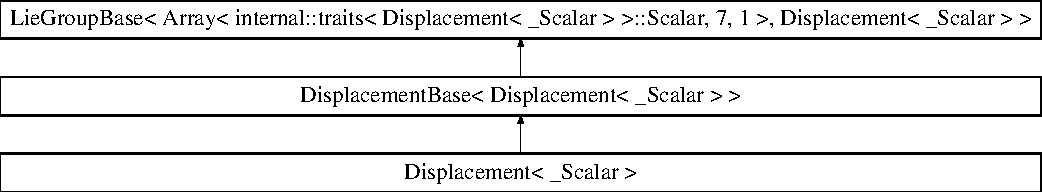
\includegraphics[height=2.584615cm]{class_displacement}
\end{center}
\end{figure}
\subsection*{Public Types}
\begin{DoxyCompactItemize}
\item 
typedef \+\_\+\+Scalar \hyperlink{class_displacement_ade979a89a65e3b67dea322a0cef92c88}{Scalar}
\item 
typedef internal\+::traits$<$ \hyperlink{class_displacement}{Displacement} $>$\+::\hyperlink{class_displacement_a995adefd20afdb476cdef2aa7bbc4531}{Coefficients} \hyperlink{class_displacement_a995adefd20afdb476cdef2aa7bbc4531}{Coefficients}
\end{DoxyCompactItemize}
\subsection*{Public Member Functions}
\begin{DoxyCompactItemize}
\item 
\hyperlink{class_displacement_a78920473a1b63b88597d9cc0e749b908}{Displacement} ()
\item 
\hyperlink{class_displacement_ac23802122cd27f1ba1f1eb70d71e5e09}{Displacement} (const \hyperlink{class_displacement}{Displacement} \&other)
\item 
{\footnotesize template$<$typename Derived $>$ }\\\hyperlink{class_displacement_a0bd84d9630e7a5c11304c07002d7ecc8}{Displacement} (const \hyperlink{class_displacement_base}{Displacement\+Base}$<$ Derived $>$ \&other)
\item 
\hyperlink{class_displacement_a252b0c985fe974b166d8d4b124ec0d5f}{Displacement} (const Array$<$ \hyperlink{class_displacement_ade979a89a65e3b67dea322a0cef92c88}{Scalar}, 7, 1 $>$ \&g)
\item 
{\footnotesize template$<$typename Derived $>$ }\\\hyperlink{class_displacement_a3b597e27e21d96f0aa0481c2a161248f}{Displacement} (const Matrix\+Base$<$ Derived $>$ \&other)
\item 
E\+I\+G\+E\+N\+\_\+\+S\+T\+R\+O\+N\+G\+\_\+\+I\+N\+L\+I\+NE \hyperlink{class_displacement_a26ee41b979d5949bab068bc3642d9828}{Displacement} (\hyperlink{class_displacement_ade979a89a65e3b67dea322a0cef92c88}{Scalar} \hyperlink{class_displacement_base_ae2b6ce0d58e72f8d36942204303960c1}{x}, \hyperlink{class_displacement_ade979a89a65e3b67dea322a0cef92c88}{Scalar} \hyperlink{class_displacement_base_ad23b504e3f85c99bd0a293aef8e823bf}{y}, \hyperlink{class_displacement_ade979a89a65e3b67dea322a0cef92c88}{Scalar} \hyperlink{class_displacement_base_ac0d87fc13d3610e764501cd857178a9f}{z}, \hyperlink{class_displacement_ade979a89a65e3b67dea322a0cef92c88}{Scalar} \hyperlink{class_displacement_base_afc5d0180532098927ad33b2ad9b91ec4}{qw}=(\hyperlink{class_displacement_ade979a89a65e3b67dea322a0cef92c88}{Scalar}) 1.\+0, \hyperlink{class_displacement_ade979a89a65e3b67dea322a0cef92c88}{Scalar} \hyperlink{class_displacement_base_ae37c8d2f1d0a6ca84550ab87dec7069d}{qx}=(\hyperlink{class_displacement_ade979a89a65e3b67dea322a0cef92c88}{Scalar}) 0.\+0, \hyperlink{class_displacement_ade979a89a65e3b67dea322a0cef92c88}{Scalar} \hyperlink{class_displacement_base_af0016b6fed409308e531b4945d60b99a}{qy}=(\hyperlink{class_displacement_ade979a89a65e3b67dea322a0cef92c88}{Scalar}) 0.\+0, \hyperlink{class_displacement_ade979a89a65e3b67dea322a0cef92c88}{Scalar} \hyperlink{class_displacement_base_a5fb14d5bda1d8531de6b6b2b05b52d5a}{qz}=(\hyperlink{class_displacement_ade979a89a65e3b67dea322a0cef92c88}{Scalar}) 0.\+0)
\item 
E\+I\+G\+E\+N\+\_\+\+S\+T\+R\+O\+N\+G\+\_\+\+I\+N\+L\+I\+NE \hyperlink{class_displacement_a65ba493ec0968d840e37f5af1a407e0e}{Displacement} (const typename \hyperlink{class_displacement_base_a0b5e3b97de6478fd98bf6aec9730d4c4}{Base\+::\+Vector3} \&v, const typename \hyperlink{class_displacement_base_aca59ea9e7f5fb3b67a489726bced7f4f}{Base\+::\+Rotation3D} \&r)
\item 
\hyperlink{class_displacement_a995adefd20afdb476cdef2aa7bbc4531}{Coefficients} \& \hyperlink{class_displacement_ac1c0567d40677f692db03770ce80b214}{get} ()
\item 
const \hyperlink{class_displacement_a995adefd20afdb476cdef2aa7bbc4531}{Coefficients} \& \hyperlink{class_displacement_adc206e570d379e6082e0cb2c7c82a41f}{get} () const
\end{DoxyCompactItemize}
\subsection*{Protected Types}
\begin{DoxyCompactItemize}
\item 
typedef \hyperlink{class_displacement_base}{Displacement\+Base}$<$ \hyperlink{class_displacement}{Displacement}$<$ \hyperlink{class_displacement_ade979a89a65e3b67dea322a0cef92c88}{Scalar} $>$ $>$ \hyperlink{class_displacement_acdd707b0e59e9f846d6c116fc8c88408}{Base}
\end{DoxyCompactItemize}
\subsection*{Protected Attributes}
\begin{DoxyCompactItemize}
\item 
\hyperlink{class_displacement_a995adefd20afdb476cdef2aa7bbc4531}{Coefficients} \hyperlink{class_displacement_aa74b681eed8e46c0df5291f32e0d7445}{m\+\_\+coeffs}
\end{DoxyCompactItemize}
\subsection*{Additional Inherited Members}


\subsection{Detailed Description}
\subsubsection*{template$<$typename \+\_\+\+Scalar$>$\newline
class Displacement$<$ \+\_\+\+Scalar $>$}

Class describing a rigid \hyperlink{class_displacement}{Displacement} or a 3D Frame position. 


\begin{DoxyTemplParams}{Template Parameters}
{\em \+\_\+\+Scalar} & the type of the underlying array\\
\hline
\end{DoxyTemplParams}
This class add some specific constructors

\begin{DoxySeeAlso}{See also}
The methods are defined in \hyperlink{class_lie_group_base}{Lie\+Group\+Base} and \hyperlink{class_displacement_base}{Displacement\+Base} 
\end{DoxySeeAlso}


Definition at line 159 of file Displacement.\+h.



\subsection{Member Typedef Documentation}
\hypertarget{class_displacement_acdd707b0e59e9f846d6c116fc8c88408}{}\label{class_displacement_acdd707b0e59e9f846d6c116fc8c88408} 
\index{Displacement@{Displacement}!Base@{Base}}
\index{Base@{Base}!Displacement@{Displacement}}
\subsubsection{\texorpdfstring{Base}{Base}}
{\footnotesize\ttfamily template$<$typename \+\_\+\+Scalar$>$ \\
typedef \hyperlink{class_displacement_base}{Displacement\+Base}$<$\hyperlink{class_displacement}{Displacement}$<$\hyperlink{class_displacement_ade979a89a65e3b67dea322a0cef92c88}{Scalar}$>$ $>$ \hyperlink{class_displacement}{Displacement}$<$ \+\_\+\+Scalar $>$\+::\hyperlink{class_displacement_acdd707b0e59e9f846d6c116fc8c88408}{Base}\hspace{0.3cm}{\ttfamily [protected]}}

The inherited class 

Definition at line 165 of file Displacement.\+h.

\hypertarget{class_displacement_a995adefd20afdb476cdef2aa7bbc4531}{}\label{class_displacement_a995adefd20afdb476cdef2aa7bbc4531} 
\index{Displacement@{Displacement}!Coefficients@{Coefficients}}
\index{Coefficients@{Coefficients}!Displacement@{Displacement}}
\subsubsection{\texorpdfstring{Coefficients}{Coefficients}}
{\footnotesize\ttfamily template$<$typename \+\_\+\+Scalar$>$ \\
typedef internal\+::traits$<$\hyperlink{class_displacement}{Displacement}$>$\+::\hyperlink{class_displacement_a995adefd20afdb476cdef2aa7bbc4531}{Coefficients} \hyperlink{class_displacement}{Displacement}$<$ \+\_\+\+Scalar $>$\+::\hyperlink{class_displacement_a995adefd20afdb476cdef2aa7bbc4531}{Coefficients}}

the stored coefficients 

Definition at line 168 of file Displacement.\+h.

\hypertarget{class_displacement_ade979a89a65e3b67dea322a0cef92c88}{}\label{class_displacement_ade979a89a65e3b67dea322a0cef92c88} 
\index{Displacement@{Displacement}!Scalar@{Scalar}}
\index{Scalar@{Scalar}!Displacement@{Displacement}}
\subsubsection{\texorpdfstring{Scalar}{Scalar}}
{\footnotesize\ttfamily template$<$typename \+\_\+\+Scalar$>$ \\
typedef \+\_\+\+Scalar \hyperlink{class_displacement}{Displacement}$<$ \+\_\+\+Scalar $>$\+::\hyperlink{class_displacement_ade979a89a65e3b67dea322a0cef92c88}{Scalar}}

The coefficients type 

Definition at line 162 of file Displacement.\+h.



\subsection{Constructor \& Destructor Documentation}
\hypertarget{class_displacement_a78920473a1b63b88597d9cc0e749b908}{}\label{class_displacement_a78920473a1b63b88597d9cc0e749b908} 
\index{Displacement@{Displacement}!Displacement@{Displacement}}
\index{Displacement@{Displacement}!Displacement@{Displacement}}
\subsubsection{\texorpdfstring{Displacement()}{Displacement()}\hspace{0.1cm}{\footnotesize\ttfamily [1/7]}}
{\footnotesize\ttfamily template$<$typename \+\_\+\+Scalar$>$ \\
\hyperlink{class_displacement}{Displacement}$<$ \+\_\+\+Scalar $>$\+::\hyperlink{class_displacement}{Displacement} (\begin{DoxyParamCaption}{ }\end{DoxyParamCaption})\hspace{0.3cm}{\ttfamily [inline]}}

Default constructor 

Definition at line 173 of file Displacement.\+h.

\hypertarget{class_displacement_ac23802122cd27f1ba1f1eb70d71e5e09}{}\label{class_displacement_ac23802122cd27f1ba1f1eb70d71e5e09} 
\index{Displacement@{Displacement}!Displacement@{Displacement}}
\index{Displacement@{Displacement}!Displacement@{Displacement}}
\subsubsection{\texorpdfstring{Displacement()}{Displacement()}\hspace{0.1cm}{\footnotesize\ttfamily [2/7]}}
{\footnotesize\ttfamily template$<$typename \+\_\+\+Scalar$>$ \\
\hyperlink{class_displacement}{Displacement}$<$ \+\_\+\+Scalar $>$\+::\hyperlink{class_displacement}{Displacement} (\begin{DoxyParamCaption}\item[{const \hyperlink{class_displacement}{Displacement}$<$ \+\_\+\+Scalar $>$ \&}]{other }\end{DoxyParamCaption})\hspace{0.3cm}{\ttfamily [inline]}}

Copy constructor 

Definition at line 175 of file Displacement.\+h.

\hypertarget{class_displacement_a0bd84d9630e7a5c11304c07002d7ecc8}{}\label{class_displacement_a0bd84d9630e7a5c11304c07002d7ecc8} 
\index{Displacement@{Displacement}!Displacement@{Displacement}}
\index{Displacement@{Displacement}!Displacement@{Displacement}}
\subsubsection{\texorpdfstring{Displacement()}{Displacement()}\hspace{0.1cm}{\footnotesize\ttfamily [3/7]}}
{\footnotesize\ttfamily template$<$typename \+\_\+\+Scalar$>$ \\
template$<$typename Derived $>$ \\
\hyperlink{class_displacement}{Displacement}$<$ \+\_\+\+Scalar $>$\+::\hyperlink{class_displacement}{Displacement} (\begin{DoxyParamCaption}\item[{const \hyperlink{class_displacement_base}{Displacement\+Base}$<$ Derived $>$ \&}]{other }\end{DoxyParamCaption})\hspace{0.3cm}{\ttfamily [inline]}}

Pseudo-\/copy constructor 

Definition at line 179 of file Displacement.\+h.

\hypertarget{class_displacement_a252b0c985fe974b166d8d4b124ec0d5f}{}\label{class_displacement_a252b0c985fe974b166d8d4b124ec0d5f} 
\index{Displacement@{Displacement}!Displacement@{Displacement}}
\index{Displacement@{Displacement}!Displacement@{Displacement}}
\subsubsection{\texorpdfstring{Displacement()}{Displacement()}\hspace{0.1cm}{\footnotesize\ttfamily [4/7]}}
{\footnotesize\ttfamily template$<$typename \+\_\+\+Scalar$>$ \\
\hyperlink{class_displacement}{Displacement}$<$ \+\_\+\+Scalar $>$\+::\hyperlink{class_displacement}{Displacement} (\begin{DoxyParamCaption}\item[{const Array$<$ \hyperlink{class_displacement_ade979a89a65e3b67dea322a0cef92c88}{Scalar}, 7, 1 $>$ \&}]{g }\end{DoxyParamCaption})\hspace{0.3cm}{\ttfamily [inline]}}

Copy constructor using the wrapped class 

Definition at line 181 of file Displacement.\+h.

\hypertarget{class_displacement_a3b597e27e21d96f0aa0481c2a161248f}{}\label{class_displacement_a3b597e27e21d96f0aa0481c2a161248f} 
\index{Displacement@{Displacement}!Displacement@{Displacement}}
\index{Displacement@{Displacement}!Displacement@{Displacement}}
\subsubsection{\texorpdfstring{Displacement()}{Displacement()}\hspace{0.1cm}{\footnotesize\ttfamily [5/7]}}
{\footnotesize\ttfamily template$<$typename \+\_\+\+Scalar$>$ \\
template$<$typename Derived $>$ \\
\hyperlink{class_displacement}{Displacement}$<$ \+\_\+\+Scalar $>$\+::\hyperlink{class_displacement}{Displacement} (\begin{DoxyParamCaption}\item[{const Matrix\+Base$<$ Derived $>$ \&}]{other }\end{DoxyParamCaption})\hspace{0.3cm}{\ttfamily [inline]}, {\ttfamily [explicit]}}



Definition at line 183 of file Displacement.\+h.

\hypertarget{class_displacement_a26ee41b979d5949bab068bc3642d9828}{}\label{class_displacement_a26ee41b979d5949bab068bc3642d9828} 
\index{Displacement@{Displacement}!Displacement@{Displacement}}
\index{Displacement@{Displacement}!Displacement@{Displacement}}
\subsubsection{\texorpdfstring{Displacement()}{Displacement()}\hspace{0.1cm}{\footnotesize\ttfamily [6/7]}}
{\footnotesize\ttfamily template$<$typename \+\_\+\+Scalar$>$ \\
E\+I\+G\+E\+N\+\_\+\+S\+T\+R\+O\+N\+G\+\_\+\+I\+N\+L\+I\+NE \hyperlink{class_displacement}{Displacement}$<$ \+\_\+\+Scalar $>$\+::\hyperlink{class_displacement}{Displacement} (\begin{DoxyParamCaption}\item[{\hyperlink{class_displacement_ade979a89a65e3b67dea322a0cef92c88}{Scalar}}]{x,  }\item[{\hyperlink{class_displacement_ade979a89a65e3b67dea322a0cef92c88}{Scalar}}]{y,  }\item[{\hyperlink{class_displacement_ade979a89a65e3b67dea322a0cef92c88}{Scalar}}]{z,  }\item[{\hyperlink{class_displacement_ade979a89a65e3b67dea322a0cef92c88}{Scalar}}]{qw = {\ttfamily (\hyperlink{class_displacement_ade979a89a65e3b67dea322a0cef92c88}{Scalar})1.0},  }\item[{\hyperlink{class_displacement_ade979a89a65e3b67dea322a0cef92c88}{Scalar}}]{qx = {\ttfamily (\hyperlink{class_displacement_ade979a89a65e3b67dea322a0cef92c88}{Scalar})0.0},  }\item[{\hyperlink{class_displacement_ade979a89a65e3b67dea322a0cef92c88}{Scalar}}]{qy = {\ttfamily (\hyperlink{class_displacement_ade979a89a65e3b67dea322a0cef92c88}{Scalar})0.0},  }\item[{\hyperlink{class_displacement_ade979a89a65e3b67dea322a0cef92c88}{Scalar}}]{qz = {\ttfamily (\hyperlink{class_displacement_ade979a89a65e3b67dea322a0cef92c88}{Scalar})0.0} }\end{DoxyParamCaption})\hspace{0.3cm}{\ttfamily [inline]}}

Constructs and initializes the displacement with $R^3$ first then $SO(3)$

\begin{DoxyWarning}{Warning}
Note the order of the arguments\+: R$^\wedge$3 first then {\ttfamily qw} (scalar part) while internally the coefficients are stored in the following order\+: \mbox{[}{\ttfamily qx}, {\ttfamily qy}, {\ttfamily qz}, {\ttfamily qw} {\ttfamily x} {\ttfamily y} {\ttfamily z}\mbox{]} 
\end{DoxyWarning}


Definition at line 190 of file Displacement.\+h.

\hypertarget{class_displacement_a65ba493ec0968d840e37f5af1a407e0e}{}\label{class_displacement_a65ba493ec0968d840e37f5af1a407e0e} 
\index{Displacement@{Displacement}!Displacement@{Displacement}}
\index{Displacement@{Displacement}!Displacement@{Displacement}}
\subsubsection{\texorpdfstring{Displacement()}{Displacement()}\hspace{0.1cm}{\footnotesize\ttfamily [7/7]}}
{\footnotesize\ttfamily template$<$typename \+\_\+\+Scalar$>$ \\
E\+I\+G\+E\+N\+\_\+\+S\+T\+R\+O\+N\+G\+\_\+\+I\+N\+L\+I\+NE \hyperlink{class_displacement}{Displacement}$<$ \+\_\+\+Scalar $>$\+::\hyperlink{class_displacement}{Displacement} (\begin{DoxyParamCaption}\item[{const typename \hyperlink{class_displacement_base_a0b5e3b97de6478fd98bf6aec9730d4c4}{Base\+::\+Vector3} \&}]{v,  }\item[{const typename \hyperlink{class_displacement_base_aca59ea9e7f5fb3b67a489726bced7f4f}{Base\+::\+Rotation3D} \&}]{r }\end{DoxyParamCaption})\hspace{0.3cm}{\ttfamily [inline]}}

Constructs a element of S\+E(3) from an element of S\+O(3) {\ttfamily r} and R$^\wedge$3 {\ttfamily v} 

Definition at line 203 of file Displacement.\+h.



\subsection{Member Function Documentation}
\hypertarget{class_displacement_ac1c0567d40677f692db03770ce80b214}{}\label{class_displacement_ac1c0567d40677f692db03770ce80b214} 
\index{Displacement@{Displacement}!get@{get}}
\index{get@{get}!Displacement@{Displacement}}
\subsubsection{\texorpdfstring{get()}{get()}\hspace{0.1cm}{\footnotesize\ttfamily [1/2]}}
{\footnotesize\ttfamily template$<$typename \+\_\+\+Scalar$>$ \\
\hyperlink{class_displacement_a995adefd20afdb476cdef2aa7bbc4531}{Coefficients}\& \hyperlink{class_displacement}{Displacement}$<$ \+\_\+\+Scalar $>$\+::get (\begin{DoxyParamCaption}{ }\end{DoxyParamCaption})\hspace{0.3cm}{\ttfamily [inline]}}

\begin{DoxyReturn}{Returns}
The stored coefficients 
\end{DoxyReturn}


Definition at line 209 of file Displacement.\+h.

\hypertarget{class_displacement_adc206e570d379e6082e0cb2c7c82a41f}{}\label{class_displacement_adc206e570d379e6082e0cb2c7c82a41f} 
\index{Displacement@{Displacement}!get@{get}}
\index{get@{get}!Displacement@{Displacement}}
\subsubsection{\texorpdfstring{get()}{get()}\hspace{0.1cm}{\footnotesize\ttfamily [2/2]}}
{\footnotesize\ttfamily template$<$typename \+\_\+\+Scalar$>$ \\
const \hyperlink{class_displacement_a995adefd20afdb476cdef2aa7bbc4531}{Coefficients}\& \hyperlink{class_displacement}{Displacement}$<$ \+\_\+\+Scalar $>$\+::get (\begin{DoxyParamCaption}{ }\end{DoxyParamCaption}) const\hspace{0.3cm}{\ttfamily [inline]}}

\begin{DoxyReturn}{Returns}
The read-\/only access to the stored coefficients 
\end{DoxyReturn}


Definition at line 211 of file Displacement.\+h.



\subsection{Member Data Documentation}
\hypertarget{class_displacement_aa74b681eed8e46c0df5291f32e0d7445}{}\label{class_displacement_aa74b681eed8e46c0df5291f32e0d7445} 
\index{Displacement@{Displacement}!m\+\_\+coeffs@{m\+\_\+coeffs}}
\index{m\+\_\+coeffs@{m\+\_\+coeffs}!Displacement@{Displacement}}
\subsubsection{\texorpdfstring{m\+\_\+coeffs}{m\_coeffs}}
{\footnotesize\ttfamily template$<$typename \+\_\+\+Scalar$>$ \\
\hyperlink{class_displacement_a995adefd20afdb476cdef2aa7bbc4531}{Coefficients} \hyperlink{class_displacement}{Displacement}$<$ \+\_\+\+Scalar $>$\+::m\+\_\+coeffs\hspace{0.3cm}{\ttfamily [protected]}}

The wrapped coefficients 

Definition at line 215 of file Displacement.\+h.



The documentation for this class was generated from the following file\+:\begin{DoxyCompactItemize}
\item 
/\+Users/\+Ryan/\+Code/codyco-\/superbuild/libraries/\+Eigen\+Lgsm/unsupported/\+Eigen/src/\+Lgsm/\hyperlink{_displacement_8h}{Displacement.\+h}\end{DoxyCompactItemize}

\hypertarget{class_displacement_base}{}\section{Displacement\+Base$<$ Derived $>$ Class Template Reference}
\label{class_displacement_base}\index{Displacement\+Base$<$ Derived $>$@{Displacement\+Base$<$ Derived $>$}}


Base class describing a rigid \hyperlink{class_displacement}{Displacement} or a 3D Frame position.  




{\ttfamily \#include $<$Displacement.\+h$>$}

Inheritance diagram for Displacement\+Base$<$ Derived $>$\+:\begin{figure}[H]
\begin{center}
\leavevmode
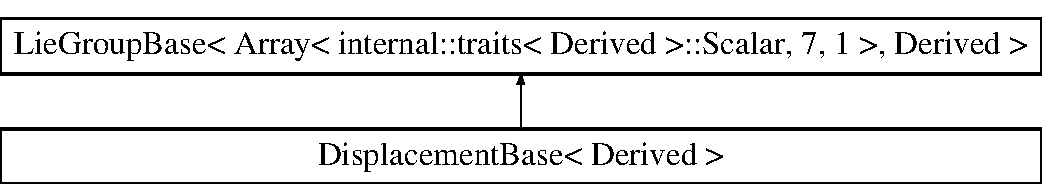
\includegraphics[height=2.000000cm]{class_displacement_base}
\end{center}
\end{figure}
\subsection*{Public Types}
\begin{DoxyCompactItemize}
\item 
typedef internal\+::traits$<$ Derived $>$\+::\hyperlink{class_displacement_base_a978caf313131fd9d221a856a2e4a80ad}{Scalar} \hyperlink{class_displacement_base_a978caf313131fd9d221a856a2e4a80ad}{Scalar}
\item 
typedef \hyperlink{class_lie_group_base_a895bed679f100c71c6dcbfd5532635b0}{Base\+::\+Base\+Type} \hyperlink{class_displacement_base_ac2d1983c0f84aa8d974283e3a48a2434}{Base\+Type}
\item 
typedef \hyperlink{class_lie_group_base_a37b1d64048a2fa65b298801f6028c468}{Base\+::\+Plain\+Object} \hyperlink{class_displacement_base_aaa66ea6d4bdfcd9ca5fbfafbc66e78b9}{Plain\+Object}
\item 
typedef Matrix$<$ \hyperlink{class_displacement_base_a978caf313131fd9d221a856a2e4a80ad}{Scalar}, 3, 1 $>$ \hyperlink{class_displacement_base_a0b5e3b97de6478fd98bf6aec9730d4c4}{Vector3}
\item 
typedef \hyperlink{class_lie_group}{Lie\+Group}$<$ Quaternion$<$ \hyperlink{class_displacement_base_a978caf313131fd9d221a856a2e4a80ad}{Scalar} $>$ $>$ \hyperlink{class_displacement_base_aca59ea9e7f5fb3b67a489726bced7f4f}{Rotation3D}
\end{DoxyCompactItemize}
\subsection*{Public Member Functions}
\begin{DoxyCompactItemize}
\item 
Map$<$ \hyperlink{class_displacement_base_aca59ea9e7f5fb3b67a489726bced7f4f}{Rotation3D} $>$ \hyperlink{class_displacement_base_a76ac4502a930ddd52833d2561a13eeb5}{get\+Rotation} ()
\item 
const Map$<$ const \hyperlink{class_displacement_base_aca59ea9e7f5fb3b67a489726bced7f4f}{Rotation3D} $>$ \hyperlink{class_displacement_base_ad13124e677c2749a7d71c5cc53c2e6a1}{get\+Rotation} () const
\item 
Map$<$ \hyperlink{class_displacement_base_a0b5e3b97de6478fd98bf6aec9730d4c4}{Vector3} $>$ \hyperlink{class_displacement_base_a034ba0c1d519c12ceeac9e72d417efb6}{get\+Translation} ()
\item 
const Map$<$ const \hyperlink{class_displacement_base_a0b5e3b97de6478fd98bf6aec9730d4c4}{Vector3} $>$ \hyperlink{class_displacement_base_a1d62cf28e94f43eef14d111c54112913}{get\+Translation} () const
\item 
\hyperlink{class_displacement_base_a978caf313131fd9d221a856a2e4a80ad}{Scalar} \hyperlink{class_displacement_base_ae2b6ce0d58e72f8d36942204303960c1}{x} () const
\item 
\hyperlink{class_displacement_base_a978caf313131fd9d221a856a2e4a80ad}{Scalar} \hyperlink{class_displacement_base_ad23b504e3f85c99bd0a293aef8e823bf}{y} () const
\item 
\hyperlink{class_displacement_base_a978caf313131fd9d221a856a2e4a80ad}{Scalar} \hyperlink{class_displacement_base_ac0d87fc13d3610e764501cd857178a9f}{z} () const
\item 
\hyperlink{class_displacement_base_a978caf313131fd9d221a856a2e4a80ad}{Scalar} \hyperlink{class_displacement_base_ae37c8d2f1d0a6ca84550ab87dec7069d}{qx} () const
\item 
\hyperlink{class_displacement_base_a978caf313131fd9d221a856a2e4a80ad}{Scalar} \hyperlink{class_displacement_base_af0016b6fed409308e531b4945d60b99a}{qy} () const
\item 
\hyperlink{class_displacement_base_a978caf313131fd9d221a856a2e4a80ad}{Scalar} \hyperlink{class_displacement_base_a5fb14d5bda1d8531de6b6b2b05b52d5a}{qz} () const
\item 
\hyperlink{class_displacement_base_a978caf313131fd9d221a856a2e4a80ad}{Scalar} \hyperlink{class_displacement_base_afc5d0180532098927ad33b2ad9b91ec4}{qw} () const
\item 
\hyperlink{class_displacement_base_a978caf313131fd9d221a856a2e4a80ad}{Scalar} \& \hyperlink{class_displacement_base_a1f29ca444e3e267eb8984cde3173d4e5}{x} ()
\item 
\hyperlink{class_displacement_base_a978caf313131fd9d221a856a2e4a80ad}{Scalar} \& \hyperlink{class_displacement_base_abe7f6f7ce47a153aec93e1b001bc700f}{y} ()
\item 
\hyperlink{class_displacement_base_a978caf313131fd9d221a856a2e4a80ad}{Scalar} \& \hyperlink{class_displacement_base_af542c09c615b88965d96397c546fcf16}{z} ()
\item 
\hyperlink{class_displacement_base_a978caf313131fd9d221a856a2e4a80ad}{Scalar} \& \hyperlink{class_displacement_base_a937faf4658311b1b17cd2e3b14ec8b15}{qx} ()
\item 
\hyperlink{class_displacement_base_a978caf313131fd9d221a856a2e4a80ad}{Scalar} \& \hyperlink{class_displacement_base_a89d0d16b7b3ea0d99f06278f83f1dc33}{qy} ()
\item 
\hyperlink{class_displacement_base_a978caf313131fd9d221a856a2e4a80ad}{Scalar} \& \hyperlink{class_displacement_base_a93797b5c38b58ef40d7c67b4cef86251}{qz} ()
\item 
\hyperlink{class_displacement_base_a978caf313131fd9d221a856a2e4a80ad}{Scalar} \& \hyperlink{class_displacement_base_a45e45394e32c27e52e10f4a5299ed13c}{qw} ()
\item 
void \hyperlink{class_displacement_base_a04542993e46456ee93c5767ad51cd1ba}{set\+Random} ()
\item 
{\footnotesize template$<$typename New\+Scalar\+Type $>$ }\\internal\+::cast\+\_\+return\+\_\+type$<$ Derived, \hyperlink{class_displacement}{Displacement}$<$ New\+Scalar\+Type $>$ $>$\+::type \hyperlink{class_displacement_base_a75e8a8cccb491a6b73ef6b2e0dd7f5db}{cast} () const
\item 
E\+I\+G\+E\+N\+\_\+\+S\+T\+R\+O\+N\+G\+\_\+\+I\+N\+L\+I\+NE \hyperlink{class_displacement_base}{Displacement\+Base} \& \hyperlink{class_displacement_base_a0fa68a3b52d098c1c9ba787e49de6fce}{operator=} (const typename \hyperlink{class_lie_group_base_a37b1d64048a2fa65b298801f6028c468}{Base\+::\+Plain\+Object} \&g)
\item 
Matrix$<$ \hyperlink{class_displacement_base_a978caf313131fd9d221a856a2e4a80ad}{Scalar}, 4, 4 $>$ \hyperlink{class_displacement_base_a4e720f3f8dde2e04033ea120a0180ba1}{to\+Homogeneous\+Matrix} () const
\end{DoxyCompactItemize}
\subsection*{Protected Types}
\begin{DoxyCompactItemize}
\item 
typedef \hyperlink{class_lie_group_base}{Lie\+Group\+Base}$<$ Array$<$ \hyperlink{class_displacement_base_a978caf313131fd9d221a856a2e4a80ad}{Scalar}, 7, 1 $>$, Derived $>$ \hyperlink{class_displacement_base_ae1eea29b955c12d84603ab1b81bfe3c4}{Base}
\end{DoxyCompactItemize}
\subsection*{Friends}
\begin{DoxyCompactItemize}
\item 
{\footnotesize template$<$class Other\+Derived $>$ }\\std\+::ostream \& \hyperlink{class_displacement_base_ae3b817959fb2c6e82221c44ff1f3c9d1}{operator$<$$<$} (std\+::ostream \&os, const \hyperlink{class_displacement_base}{Displacement\+Base}$<$ Other\+Derived $>$ \&d)
\end{DoxyCompactItemize}
\subsection*{Additional Inherited Members}


\subsection{Detailed Description}
\subsubsection*{template$<$class Derived$>$\newline
class Displacement\+Base$<$ Derived $>$}

Base class describing a rigid \hyperlink{class_displacement}{Displacement} or a 3D Frame position. 


\begin{DoxyTemplParams}{Template Parameters}
{\em Derived} & the derived class holding the coefficients which are of type Array$<$\+Scalar, 7, 1$>$ or Map$<$Array$<$\+Scalar, 7, 1$>$ $>$\\
\hline
\end{DoxyTemplParams}
This class abstracts the underlying mathematical definition and add some accessors. It uses an Array internally to store its coefficients. 

Definition at line 28 of file Displacement.\+h.



\subsection{Member Typedef Documentation}
\hypertarget{class_displacement_base_ae1eea29b955c12d84603ab1b81bfe3c4}{}\label{class_displacement_base_ae1eea29b955c12d84603ab1b81bfe3c4} 
\index{Displacement\+Base@{Displacement\+Base}!Base@{Base}}
\index{Base@{Base}!Displacement\+Base@{Displacement\+Base}}
\subsubsection{\texorpdfstring{Base}{Base}}
{\footnotesize\ttfamily template$<$class Derived$>$ \\
typedef \hyperlink{class_lie_group_base}{Lie\+Group\+Base}$<$Array$<$\hyperlink{class_displacement_base_a978caf313131fd9d221a856a2e4a80ad}{Scalar}, 7, 1$>$, Derived$>$ \hyperlink{class_displacement_base}{Displacement\+Base}$<$ Derived $>$\+::\hyperlink{class_displacement_base_ae1eea29b955c12d84603ab1b81bfe3c4}{Base}\hspace{0.3cm}{\ttfamily [protected]}}

The inherited class 

Definition at line 34 of file Displacement.\+h.

\hypertarget{class_displacement_base_ac2d1983c0f84aa8d974283e3a48a2434}{}\label{class_displacement_base_ac2d1983c0f84aa8d974283e3a48a2434} 
\index{Displacement\+Base@{Displacement\+Base}!Base\+Type@{Base\+Type}}
\index{Base\+Type@{Base\+Type}!Displacement\+Base@{Displacement\+Base}}
\subsubsection{\texorpdfstring{Base\+Type}{BaseType}}
{\footnotesize\ttfamily template$<$class Derived$>$ \\
typedef \hyperlink{class_lie_group_base_a895bed679f100c71c6dcbfd5532635b0}{Base\+::\+Base\+Type} \hyperlink{class_displacement_base}{Displacement\+Base}$<$ Derived $>$\+::\hyperlink{class_displacement_base_ac2d1983c0f84aa8d974283e3a48a2434}{Base\+Type}}

The wrapped class (Array$<$\+Scalar, 7, 1$>$ 

Definition at line 40 of file Displacement.\+h.

\hypertarget{class_displacement_base_aaa66ea6d4bdfcd9ca5fbfafbc66e78b9}{}\label{class_displacement_base_aaa66ea6d4bdfcd9ca5fbfafbc66e78b9} 
\index{Displacement\+Base@{Displacement\+Base}!Plain\+Object@{Plain\+Object}}
\index{Plain\+Object@{Plain\+Object}!Displacement\+Base@{Displacement\+Base}}
\subsubsection{\texorpdfstring{Plain\+Object}{PlainObject}}
{\footnotesize\ttfamily template$<$class Derived$>$ \\
typedef \hyperlink{class_lie_group_base_a37b1d64048a2fa65b298801f6028c468}{Base\+::\+Plain\+Object} \hyperlink{class_displacement_base}{Displacement\+Base}$<$ Derived $>$\+::\hyperlink{class_displacement_base_aaa66ea6d4bdfcd9ca5fbfafbc66e78b9}{Plain\+Object}}

The plain object returned, while using Map$<$\+Displacement $>$ 

Definition at line 42 of file Displacement.\+h.

\hypertarget{class_displacement_base_aca59ea9e7f5fb3b67a489726bced7f4f}{}\label{class_displacement_base_aca59ea9e7f5fb3b67a489726bced7f4f} 
\index{Displacement\+Base@{Displacement\+Base}!Rotation3D@{Rotation3D}}
\index{Rotation3D@{Rotation3D}!Displacement\+Base@{Displacement\+Base}}
\subsubsection{\texorpdfstring{Rotation3D}{Rotation3D}}
{\footnotesize\ttfamily template$<$class Derived$>$ \\
typedef \hyperlink{class_lie_group}{Lie\+Group}$<$Quaternion$<$\hyperlink{class_displacement_base_a978caf313131fd9d221a856a2e4a80ad}{Scalar}$>$ $>$ \hyperlink{class_displacement_base}{Displacement\+Base}$<$ Derived $>$\+::\hyperlink{class_displacement_base_aca59ea9e7f5fb3b67a489726bced7f4f}{Rotation3D}}

The type of the rotation part 

Definition at line 47 of file Displacement.\+h.

\hypertarget{class_displacement_base_a978caf313131fd9d221a856a2e4a80ad}{}\label{class_displacement_base_a978caf313131fd9d221a856a2e4a80ad} 
\index{Displacement\+Base@{Displacement\+Base}!Scalar@{Scalar}}
\index{Scalar@{Scalar}!Displacement\+Base@{Displacement\+Base}}
\subsubsection{\texorpdfstring{Scalar}{Scalar}}
{\footnotesize\ttfamily template$<$class Derived$>$ \\
typedef internal\+::traits$<$Derived$>$\+::\hyperlink{class_displacement_base_a978caf313131fd9d221a856a2e4a80ad}{Scalar} \hyperlink{class_displacement_base}{Displacement\+Base}$<$ Derived $>$\+::\hyperlink{class_displacement_base_a978caf313131fd9d221a856a2e4a80ad}{Scalar}}

The coefficients type 

Definition at line 31 of file Displacement.\+h.

\hypertarget{class_displacement_base_a0b5e3b97de6478fd98bf6aec9730d4c4}{}\label{class_displacement_base_a0b5e3b97de6478fd98bf6aec9730d4c4} 
\index{Displacement\+Base@{Displacement\+Base}!Vector3@{Vector3}}
\index{Vector3@{Vector3}!Displacement\+Base@{Displacement\+Base}}
\subsubsection{\texorpdfstring{Vector3}{Vector3}}
{\footnotesize\ttfamily template$<$class Derived$>$ \\
typedef Matrix$<$\hyperlink{class_displacement_base_a978caf313131fd9d221a856a2e4a80ad}{Scalar}, 3, 1$>$ \hyperlink{class_displacement_base}{Displacement\+Base}$<$ Derived $>$\+::\hyperlink{class_displacement_base_a0b5e3b97de6478fd98bf6aec9730d4c4}{Vector3}}

The type of the translation part 

Definition at line 45 of file Displacement.\+h.



\subsection{Member Function Documentation}
\hypertarget{class_displacement_base_a75e8a8cccb491a6b73ef6b2e0dd7f5db}{}\label{class_displacement_base_a75e8a8cccb491a6b73ef6b2e0dd7f5db} 
\index{Displacement\+Base@{Displacement\+Base}!cast@{cast}}
\index{cast@{cast}!Displacement\+Base@{Displacement\+Base}}
\subsubsection{\texorpdfstring{cast()}{cast()}}
{\footnotesize\ttfamily template$<$class Derived$>$ \\
template$<$typename New\+Scalar\+Type $>$ \\
internal\+::cast\+\_\+return\+\_\+type$<$Derived, \hyperlink{class_displacement}{Displacement}$<$New\+Scalar\+Type$>$ $>$\+::type \hyperlink{class_displacement_base}{Displacement\+Base}$<$ Derived $>$\+::cast (\begin{DoxyParamCaption}{ }\end{DoxyParamCaption}) const\hspace{0.3cm}{\ttfamily [inline]}}

\begin{DoxyReturn}{Returns}
{\ttfamily $\ast$this} with scalar type casted to {\itshape New\+Scalar\+Type} 
\end{DoxyReturn}
Note that if {\itshape New\+Scalar\+Type} is equal to the current scalar type of {\ttfamily $\ast$this} then this function smartly returns a const reference to {\ttfamily $\ast$this}. 

Definition at line 100 of file Displacement.\+h.

\hypertarget{class_displacement_base_a76ac4502a930ddd52833d2561a13eeb5}{}\label{class_displacement_base_a76ac4502a930ddd52833d2561a13eeb5} 
\index{Displacement\+Base@{Displacement\+Base}!get\+Rotation@{get\+Rotation}}
\index{get\+Rotation@{get\+Rotation}!Displacement\+Base@{Displacement\+Base}}
\subsubsection{\texorpdfstring{get\+Rotation()}{getRotation()}\hspace{0.1cm}{\footnotesize\ttfamily [1/2]}}
{\footnotesize\ttfamily template$<$class Derived$>$ \\
Map$<$\hyperlink{class_displacement_base_aca59ea9e7f5fb3b67a489726bced7f4f}{Rotation3D}$>$ \hyperlink{class_displacement_base}{Displacement\+Base}$<$ Derived $>$\+::get\+Rotation (\begin{DoxyParamCaption}{ }\end{DoxyParamCaption})\hspace{0.3cm}{\ttfamily [inline]}}

The accessor to the rotation part 

Definition at line 50 of file Displacement.\+h.

\hypertarget{class_displacement_base_ad13124e677c2749a7d71c5cc53c2e6a1}{}\label{class_displacement_base_ad13124e677c2749a7d71c5cc53c2e6a1} 
\index{Displacement\+Base@{Displacement\+Base}!get\+Rotation@{get\+Rotation}}
\index{get\+Rotation@{get\+Rotation}!Displacement\+Base@{Displacement\+Base}}
\subsubsection{\texorpdfstring{get\+Rotation()}{getRotation()}\hspace{0.1cm}{\footnotesize\ttfamily [2/2]}}
{\footnotesize\ttfamily template$<$class Derived$>$ \\
const Map$<$const \hyperlink{class_displacement_base_aca59ea9e7f5fb3b67a489726bced7f4f}{Rotation3D}$>$ \hyperlink{class_displacement_base}{Displacement\+Base}$<$ Derived $>$\+::get\+Rotation (\begin{DoxyParamCaption}{ }\end{DoxyParamCaption}) const\hspace{0.3cm}{\ttfamily [inline]}}

The read-\/only accessor to the rotation part 

Definition at line 52 of file Displacement.\+h.

\hypertarget{class_displacement_base_a034ba0c1d519c12ceeac9e72d417efb6}{}\label{class_displacement_base_a034ba0c1d519c12ceeac9e72d417efb6} 
\index{Displacement\+Base@{Displacement\+Base}!get\+Translation@{get\+Translation}}
\index{get\+Translation@{get\+Translation}!Displacement\+Base@{Displacement\+Base}}
\subsubsection{\texorpdfstring{get\+Translation()}{getTranslation()}\hspace{0.1cm}{\footnotesize\ttfamily [1/2]}}
{\footnotesize\ttfamily template$<$class Derived$>$ \\
Map$<$\hyperlink{class_displacement_base_a0b5e3b97de6478fd98bf6aec9730d4c4}{Vector3}$>$ \hyperlink{class_displacement_base}{Displacement\+Base}$<$ Derived $>$\+::get\+Translation (\begin{DoxyParamCaption}{ }\end{DoxyParamCaption})\hspace{0.3cm}{\ttfamily [inline]}}

The accessor to the translation part 

Definition at line 54 of file Displacement.\+h.

\hypertarget{class_displacement_base_a1d62cf28e94f43eef14d111c54112913}{}\label{class_displacement_base_a1d62cf28e94f43eef14d111c54112913} 
\index{Displacement\+Base@{Displacement\+Base}!get\+Translation@{get\+Translation}}
\index{get\+Translation@{get\+Translation}!Displacement\+Base@{Displacement\+Base}}
\subsubsection{\texorpdfstring{get\+Translation()}{getTranslation()}\hspace{0.1cm}{\footnotesize\ttfamily [2/2]}}
{\footnotesize\ttfamily template$<$class Derived$>$ \\
const Map$<$const \hyperlink{class_displacement_base_a0b5e3b97de6478fd98bf6aec9730d4c4}{Vector3}$>$ \hyperlink{class_displacement_base}{Displacement\+Base}$<$ Derived $>$\+::get\+Translation (\begin{DoxyParamCaption}{ }\end{DoxyParamCaption}) const\hspace{0.3cm}{\ttfamily [inline]}}

The read-\/only accessor to the translation part 

Definition at line 56 of file Displacement.\+h.

\hypertarget{class_displacement_base_a0fa68a3b52d098c1c9ba787e49de6fce}{}\label{class_displacement_base_a0fa68a3b52d098c1c9ba787e49de6fce} 
\index{Displacement\+Base@{Displacement\+Base}!operator=@{operator=}}
\index{operator=@{operator=}!Displacement\+Base@{Displacement\+Base}}
\subsubsection{\texorpdfstring{operator=()}{operator=()}}
{\footnotesize\ttfamily template$<$class Derived$>$ \\
E\+I\+G\+E\+N\+\_\+\+S\+T\+R\+O\+N\+G\+\_\+\+I\+N\+L\+I\+NE \hyperlink{class_displacement_base}{Displacement\+Base}\& \hyperlink{class_displacement_base}{Displacement\+Base}$<$ Derived $>$\+::operator= (\begin{DoxyParamCaption}\item[{const typename \hyperlink{class_lie_group_base_a37b1d64048a2fa65b298801f6028c468}{Base\+::\+Plain\+Object} \&}]{g }\end{DoxyParamCaption})\hspace{0.3cm}{\ttfamily [inline]}}



Definition at line 106 of file Displacement.\+h.

\hypertarget{class_displacement_base_afc5d0180532098927ad33b2ad9b91ec4}{}\label{class_displacement_base_afc5d0180532098927ad33b2ad9b91ec4} 
\index{Displacement\+Base@{Displacement\+Base}!qw@{qw}}
\index{qw@{qw}!Displacement\+Base@{Displacement\+Base}}
\subsubsection{\texorpdfstring{qw()}{qw()}\hspace{0.1cm}{\footnotesize\ttfamily [1/2]}}
{\footnotesize\ttfamily template$<$class Derived$>$ \\
\hyperlink{class_displacement_base_a978caf313131fd9d221a856a2e4a80ad}{Scalar} \hyperlink{class_displacement_base}{Displacement\+Base}$<$ Derived $>$\+::qw (\begin{DoxyParamCaption}{ }\end{DoxyParamCaption}) const\hspace{0.3cm}{\ttfamily [inline]}}

\begin{DoxyReturn}{Returns}
the {\ttfamily qw} coefficient 
\end{DoxyReturn}


Definition at line 72 of file Displacement.\+h.

\hypertarget{class_displacement_base_a45e45394e32c27e52e10f4a5299ed13c}{}\label{class_displacement_base_a45e45394e32c27e52e10f4a5299ed13c} 
\index{Displacement\+Base@{Displacement\+Base}!qw@{qw}}
\index{qw@{qw}!Displacement\+Base@{Displacement\+Base}}
\subsubsection{\texorpdfstring{qw()}{qw()}\hspace{0.1cm}{\footnotesize\ttfamily [2/2]}}
{\footnotesize\ttfamily template$<$class Derived$>$ \\
\hyperlink{class_displacement_base_a978caf313131fd9d221a856a2e4a80ad}{Scalar}\& \hyperlink{class_displacement_base}{Displacement\+Base}$<$ Derived $>$\+::qw (\begin{DoxyParamCaption}{ }\end{DoxyParamCaption})\hspace{0.3cm}{\ttfamily [inline]}}

\begin{DoxyReturn}{Returns}
a reference to the {\ttfamily qw} coefficient 
\end{DoxyReturn}


Definition at line 87 of file Displacement.\+h.

\hypertarget{class_displacement_base_ae37c8d2f1d0a6ca84550ab87dec7069d}{}\label{class_displacement_base_ae37c8d2f1d0a6ca84550ab87dec7069d} 
\index{Displacement\+Base@{Displacement\+Base}!qx@{qx}}
\index{qx@{qx}!Displacement\+Base@{Displacement\+Base}}
\subsubsection{\texorpdfstring{qx()}{qx()}\hspace{0.1cm}{\footnotesize\ttfamily [1/2]}}
{\footnotesize\ttfamily template$<$class Derived$>$ \\
\hyperlink{class_displacement_base_a978caf313131fd9d221a856a2e4a80ad}{Scalar} \hyperlink{class_displacement_base}{Displacement\+Base}$<$ Derived $>$\+::qx (\begin{DoxyParamCaption}{ }\end{DoxyParamCaption}) const\hspace{0.3cm}{\ttfamily [inline]}}

\begin{DoxyReturn}{Returns}
the {\ttfamily qx} coefficient 
\end{DoxyReturn}


Definition at line 66 of file Displacement.\+h.

\hypertarget{class_displacement_base_a937faf4658311b1b17cd2e3b14ec8b15}{}\label{class_displacement_base_a937faf4658311b1b17cd2e3b14ec8b15} 
\index{Displacement\+Base@{Displacement\+Base}!qx@{qx}}
\index{qx@{qx}!Displacement\+Base@{Displacement\+Base}}
\subsubsection{\texorpdfstring{qx()}{qx()}\hspace{0.1cm}{\footnotesize\ttfamily [2/2]}}
{\footnotesize\ttfamily template$<$class Derived$>$ \\
\hyperlink{class_displacement_base_a978caf313131fd9d221a856a2e4a80ad}{Scalar}\& \hyperlink{class_displacement_base}{Displacement\+Base}$<$ Derived $>$\+::qx (\begin{DoxyParamCaption}{ }\end{DoxyParamCaption})\hspace{0.3cm}{\ttfamily [inline]}}

\begin{DoxyReturn}{Returns}
a reference to the {\ttfamily qx} coefficient 
\end{DoxyReturn}


Definition at line 81 of file Displacement.\+h.

\hypertarget{class_displacement_base_af0016b6fed409308e531b4945d60b99a}{}\label{class_displacement_base_af0016b6fed409308e531b4945d60b99a} 
\index{Displacement\+Base@{Displacement\+Base}!qy@{qy}}
\index{qy@{qy}!Displacement\+Base@{Displacement\+Base}}
\subsubsection{\texorpdfstring{qy()}{qy()}\hspace{0.1cm}{\footnotesize\ttfamily [1/2]}}
{\footnotesize\ttfamily template$<$class Derived$>$ \\
\hyperlink{class_displacement_base_a978caf313131fd9d221a856a2e4a80ad}{Scalar} \hyperlink{class_displacement_base}{Displacement\+Base}$<$ Derived $>$\+::qy (\begin{DoxyParamCaption}{ }\end{DoxyParamCaption}) const\hspace{0.3cm}{\ttfamily [inline]}}

\begin{DoxyReturn}{Returns}
the {\ttfamily qy} coefficient 
\end{DoxyReturn}


Definition at line 68 of file Displacement.\+h.

\hypertarget{class_displacement_base_a89d0d16b7b3ea0d99f06278f83f1dc33}{}\label{class_displacement_base_a89d0d16b7b3ea0d99f06278f83f1dc33} 
\index{Displacement\+Base@{Displacement\+Base}!qy@{qy}}
\index{qy@{qy}!Displacement\+Base@{Displacement\+Base}}
\subsubsection{\texorpdfstring{qy()}{qy()}\hspace{0.1cm}{\footnotesize\ttfamily [2/2]}}
{\footnotesize\ttfamily template$<$class Derived$>$ \\
\hyperlink{class_displacement_base_a978caf313131fd9d221a856a2e4a80ad}{Scalar}\& \hyperlink{class_displacement_base}{Displacement\+Base}$<$ Derived $>$\+::qy (\begin{DoxyParamCaption}{ }\end{DoxyParamCaption})\hspace{0.3cm}{\ttfamily [inline]}}

\begin{DoxyReturn}{Returns}
a reference to the {\ttfamily qy} coefficient 
\end{DoxyReturn}


Definition at line 83 of file Displacement.\+h.

\hypertarget{class_displacement_base_a5fb14d5bda1d8531de6b6b2b05b52d5a}{}\label{class_displacement_base_a5fb14d5bda1d8531de6b6b2b05b52d5a} 
\index{Displacement\+Base@{Displacement\+Base}!qz@{qz}}
\index{qz@{qz}!Displacement\+Base@{Displacement\+Base}}
\subsubsection{\texorpdfstring{qz()}{qz()}\hspace{0.1cm}{\footnotesize\ttfamily [1/2]}}
{\footnotesize\ttfamily template$<$class Derived$>$ \\
\hyperlink{class_displacement_base_a978caf313131fd9d221a856a2e4a80ad}{Scalar} \hyperlink{class_displacement_base}{Displacement\+Base}$<$ Derived $>$\+::qz (\begin{DoxyParamCaption}{ }\end{DoxyParamCaption}) const\hspace{0.3cm}{\ttfamily [inline]}}

\begin{DoxyReturn}{Returns}
the {\ttfamily qz} coefficient 
\end{DoxyReturn}


Definition at line 70 of file Displacement.\+h.

\hypertarget{class_displacement_base_a93797b5c38b58ef40d7c67b4cef86251}{}\label{class_displacement_base_a93797b5c38b58ef40d7c67b4cef86251} 
\index{Displacement\+Base@{Displacement\+Base}!qz@{qz}}
\index{qz@{qz}!Displacement\+Base@{Displacement\+Base}}
\subsubsection{\texorpdfstring{qz()}{qz()}\hspace{0.1cm}{\footnotesize\ttfamily [2/2]}}
{\footnotesize\ttfamily template$<$class Derived$>$ \\
\hyperlink{class_displacement_base_a978caf313131fd9d221a856a2e4a80ad}{Scalar}\& \hyperlink{class_displacement_base}{Displacement\+Base}$<$ Derived $>$\+::qz (\begin{DoxyParamCaption}{ }\end{DoxyParamCaption})\hspace{0.3cm}{\ttfamily [inline]}}

\begin{DoxyReturn}{Returns}
a reference to the {\ttfamily qz} coefficient 
\end{DoxyReturn}


Definition at line 85 of file Displacement.\+h.

\hypertarget{class_displacement_base_a04542993e46456ee93c5767ad51cd1ba}{}\label{class_displacement_base_a04542993e46456ee93c5767ad51cd1ba} 
\index{Displacement\+Base@{Displacement\+Base}!set\+Random@{set\+Random}}
\index{set\+Random@{set\+Random}!Displacement\+Base@{Displacement\+Base}}
\subsubsection{\texorpdfstring{set\+Random()}{setRandom()}}
{\footnotesize\ttfamily template$<$class Derived$>$ \\
void \hyperlink{class_displacement_base}{Displacement\+Base}$<$ Derived $>$\+::set\+Random (\begin{DoxyParamCaption}{ }\end{DoxyParamCaption})\hspace{0.3cm}{\ttfamily [inline]}}



Definition at line 89 of file Displacement.\+h.

\hypertarget{class_displacement_base_a4e720f3f8dde2e04033ea120a0180ba1}{}\label{class_displacement_base_a4e720f3f8dde2e04033ea120a0180ba1} 
\index{Displacement\+Base@{Displacement\+Base}!to\+Homogeneous\+Matrix@{to\+Homogeneous\+Matrix}}
\index{to\+Homogeneous\+Matrix@{to\+Homogeneous\+Matrix}!Displacement\+Base@{Displacement\+Base}}
\subsubsection{\texorpdfstring{to\+Homogeneous\+Matrix()}{toHomogeneousMatrix()}}
{\footnotesize\ttfamily template$<$class Derived $>$ \\
Matrix$<$ typename internal\+::traits$<$ Derived $>$\+::\hyperlink{class_displacement_base_a978caf313131fd9d221a856a2e4a80ad}{Scalar}, 4, 4 $>$ \hyperlink{class_displacement_base}{Displacement\+Base}$<$ Derived $>$\+::to\+Homogeneous\+Matrix (\begin{DoxyParamCaption}{ }\end{DoxyParamCaption}) const}



Definition at line 119 of file Displacement.\+h.

\hypertarget{class_displacement_base_ae2b6ce0d58e72f8d36942204303960c1}{}\label{class_displacement_base_ae2b6ce0d58e72f8d36942204303960c1} 
\index{Displacement\+Base@{Displacement\+Base}!x@{x}}
\index{x@{x}!Displacement\+Base@{Displacement\+Base}}
\subsubsection{\texorpdfstring{x()}{x()}\hspace{0.1cm}{\footnotesize\ttfamily [1/2]}}
{\footnotesize\ttfamily template$<$class Derived$>$ \\
\hyperlink{class_displacement_base_a978caf313131fd9d221a856a2e4a80ad}{Scalar} \hyperlink{class_displacement_base}{Displacement\+Base}$<$ Derived $>$\+::x (\begin{DoxyParamCaption}{ }\end{DoxyParamCaption}) const\hspace{0.3cm}{\ttfamily [inline]}}

\begin{DoxyReturn}{Returns}
the {\ttfamily x} coefficient 
\end{DoxyReturn}


Definition at line 60 of file Displacement.\+h.

\hypertarget{class_displacement_base_a1f29ca444e3e267eb8984cde3173d4e5}{}\label{class_displacement_base_a1f29ca444e3e267eb8984cde3173d4e5} 
\index{Displacement\+Base@{Displacement\+Base}!x@{x}}
\index{x@{x}!Displacement\+Base@{Displacement\+Base}}
\subsubsection{\texorpdfstring{x()}{x()}\hspace{0.1cm}{\footnotesize\ttfamily [2/2]}}
{\footnotesize\ttfamily template$<$class Derived$>$ \\
\hyperlink{class_displacement_base_a978caf313131fd9d221a856a2e4a80ad}{Scalar}\& \hyperlink{class_displacement_base}{Displacement\+Base}$<$ Derived $>$\+::x (\begin{DoxyParamCaption}{ }\end{DoxyParamCaption})\hspace{0.3cm}{\ttfamily [inline]}}

\begin{DoxyReturn}{Returns}
a reference to the {\ttfamily x} coefficient 
\end{DoxyReturn}


Definition at line 75 of file Displacement.\+h.

\hypertarget{class_displacement_base_ad23b504e3f85c99bd0a293aef8e823bf}{}\label{class_displacement_base_ad23b504e3f85c99bd0a293aef8e823bf} 
\index{Displacement\+Base@{Displacement\+Base}!y@{y}}
\index{y@{y}!Displacement\+Base@{Displacement\+Base}}
\subsubsection{\texorpdfstring{y()}{y()}\hspace{0.1cm}{\footnotesize\ttfamily [1/2]}}
{\footnotesize\ttfamily template$<$class Derived$>$ \\
\hyperlink{class_displacement_base_a978caf313131fd9d221a856a2e4a80ad}{Scalar} \hyperlink{class_displacement_base}{Displacement\+Base}$<$ Derived $>$\+::y (\begin{DoxyParamCaption}{ }\end{DoxyParamCaption}) const\hspace{0.3cm}{\ttfamily [inline]}}

\begin{DoxyReturn}{Returns}
the {\ttfamily y} coefficient 
\end{DoxyReturn}


Definition at line 62 of file Displacement.\+h.

\hypertarget{class_displacement_base_abe7f6f7ce47a153aec93e1b001bc700f}{}\label{class_displacement_base_abe7f6f7ce47a153aec93e1b001bc700f} 
\index{Displacement\+Base@{Displacement\+Base}!y@{y}}
\index{y@{y}!Displacement\+Base@{Displacement\+Base}}
\subsubsection{\texorpdfstring{y()}{y()}\hspace{0.1cm}{\footnotesize\ttfamily [2/2]}}
{\footnotesize\ttfamily template$<$class Derived$>$ \\
\hyperlink{class_displacement_base_a978caf313131fd9d221a856a2e4a80ad}{Scalar}\& \hyperlink{class_displacement_base}{Displacement\+Base}$<$ Derived $>$\+::y (\begin{DoxyParamCaption}{ }\end{DoxyParamCaption})\hspace{0.3cm}{\ttfamily [inline]}}

\begin{DoxyReturn}{Returns}
a reference to the {\ttfamily y} coefficient 
\end{DoxyReturn}


Definition at line 77 of file Displacement.\+h.

\hypertarget{class_displacement_base_ac0d87fc13d3610e764501cd857178a9f}{}\label{class_displacement_base_ac0d87fc13d3610e764501cd857178a9f} 
\index{Displacement\+Base@{Displacement\+Base}!z@{z}}
\index{z@{z}!Displacement\+Base@{Displacement\+Base}}
\subsubsection{\texorpdfstring{z()}{z()}\hspace{0.1cm}{\footnotesize\ttfamily [1/2]}}
{\footnotesize\ttfamily template$<$class Derived$>$ \\
\hyperlink{class_displacement_base_a978caf313131fd9d221a856a2e4a80ad}{Scalar} \hyperlink{class_displacement_base}{Displacement\+Base}$<$ Derived $>$\+::z (\begin{DoxyParamCaption}{ }\end{DoxyParamCaption}) const\hspace{0.3cm}{\ttfamily [inline]}}

\begin{DoxyReturn}{Returns}
the {\ttfamily z} coefficient 
\end{DoxyReturn}


Definition at line 64 of file Displacement.\+h.

\hypertarget{class_displacement_base_af542c09c615b88965d96397c546fcf16}{}\label{class_displacement_base_af542c09c615b88965d96397c546fcf16} 
\index{Displacement\+Base@{Displacement\+Base}!z@{z}}
\index{z@{z}!Displacement\+Base@{Displacement\+Base}}
\subsubsection{\texorpdfstring{z()}{z()}\hspace{0.1cm}{\footnotesize\ttfamily [2/2]}}
{\footnotesize\ttfamily template$<$class Derived$>$ \\
\hyperlink{class_displacement_base_a978caf313131fd9d221a856a2e4a80ad}{Scalar}\& \hyperlink{class_displacement_base}{Displacement\+Base}$<$ Derived $>$\+::z (\begin{DoxyParamCaption}{ }\end{DoxyParamCaption})\hspace{0.3cm}{\ttfamily [inline]}}

\begin{DoxyReturn}{Returns}
a reference to the {\ttfamily z} coefficient 
\end{DoxyReturn}


Definition at line 79 of file Displacement.\+h.



\subsection{Friends And Related Function Documentation}
\hypertarget{class_displacement_base_ae3b817959fb2c6e82221c44ff1f3c9d1}{}\label{class_displacement_base_ae3b817959fb2c6e82221c44ff1f3c9d1} 
\index{Displacement\+Base@{Displacement\+Base}!operator$<$$<$@{operator$<$$<$}}
\index{operator$<$$<$@{operator$<$$<$}!Displacement\+Base@{Displacement\+Base}}
\subsubsection{\texorpdfstring{operator$<$$<$}{operator<<}}
{\footnotesize\ttfamily template$<$class Derived$>$ \\
template$<$class Other\+Derived $>$ \\
std\+::ostream\& operator$<$$<$ (\begin{DoxyParamCaption}\item[{std\+::ostream \&}]{os,  }\item[{const \hyperlink{class_displacement_base}{Displacement\+Base}$<$ Other\+Derived $>$ \&}]{d }\end{DoxyParamCaption})\hspace{0.3cm}{\ttfamily [friend]}}

Outputs to the given stream \+: order \+: w x y z (it\textquotesingle{}s different from the storage order) 

The documentation for this class was generated from the following file\+:\begin{DoxyCompactItemize}
\item 
/\+Users/\+Ryan/\+Code/codyco-\/superbuild/libraries/\+Eigen\+Lgsm/unsupported/\+Eigen/src/\+Lgsm/\hyperlink{_displacement_8h}{Displacement.\+h}\end{DoxyCompactItemize}

\hypertarget{class_lie_algebra}{}\section{Lie\+Algebra$<$ A $>$ Class Template Reference}
\label{class_lie_algebra}\index{Lie\+Algebra$<$ A $>$@{Lie\+Algebra$<$ A $>$}}


Class describing an element of a Lie Algebra.  




{\ttfamily \#include $<$Lie\+Algebra.\+h$>$}

Inheritance diagram for Lie\+Algebra$<$ A $>$\+:\begin{figure}[H]
\begin{center}
\leavevmode
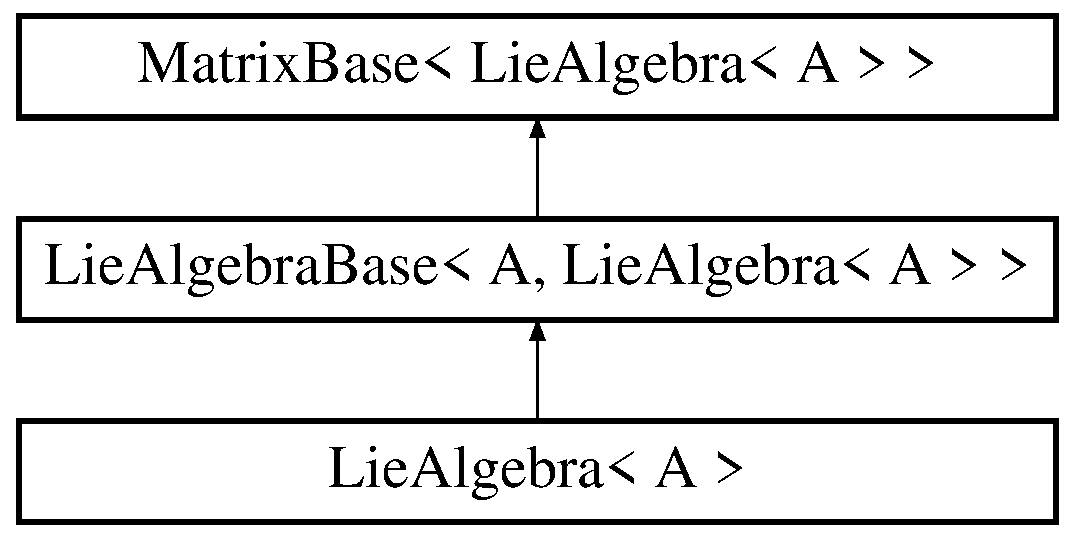
\includegraphics[height=3.000000cm]{class_lie_algebra}
\end{center}
\end{figure}
\subsection*{Public Types}
\begin{DoxyCompactItemize}
\item 
typedef internal\+::traits$<$ \hyperlink{class_lie_algebra}{Lie\+Algebra}$<$ A $>$ $>$\+::\hyperlink{class_lie_algebra_a366fde92cd31cf93be87fe82952c8ebb}{Coefficients} \hyperlink{class_lie_algebra_a366fde92cd31cf93be87fe82952c8ebb}{Coefficients}
\end{DoxyCompactItemize}
\subsection*{Public Member Functions}
\begin{DoxyCompactItemize}
\item 
\hyperlink{class_lie_algebra_ac04b1456c7a78d070a6672b8f7989197}{Lie\+Algebra} (const \hyperlink{class_lie_algebra}{Lie\+Algebra} \&)
\item 
\hyperlink{class_lie_algebra_a366fde92cd31cf93be87fe82952c8ebb}{Coefficients} \& \hyperlink{class_lie_algebra_a5d64201eddce6b2124890c26a684fc8f}{get} ()
\item 
const \hyperlink{class_lie_algebra_a366fde92cd31cf93be87fe82952c8ebb}{Coefficients} \& \hyperlink{class_lie_algebra_aa90c4e53102c2376bf24af1cb4f0112c}{get} () const
\end{DoxyCompactItemize}
\subsection*{Protected Types}
\begin{DoxyCompactItemize}
\item 
typedef \hyperlink{class_lie_algebra_base}{Lie\+Algebra\+Base}$<$ A, \hyperlink{class_lie_algebra}{Lie\+Algebra}$<$ A $>$ $>$ \hyperlink{class_lie_algebra_a28bc019eb9b070751abe554b0de567f4}{Base}
\end{DoxyCompactItemize}
\subsection*{Protected Attributes}
\begin{DoxyCompactItemize}
\item 
\hyperlink{class_lie_algebra_a366fde92cd31cf93be87fe82952c8ebb}{Coefficients} \hyperlink{class_lie_algebra_a00c8e1711af4458171c63741aec83ffc}{m\+\_\+coeffs}
\end{DoxyCompactItemize}


\subsection{Detailed Description}
\subsubsection*{template$<$class A$>$\newline
class Lie\+Algebra$<$ A $>$}

Class describing an element of a Lie Algebra. 


\begin{DoxyTemplParams}{Template Parameters}
{\em A} & the wrapped class\\
\hline
\end{DoxyTemplParams}
This class must be specialized to add new constructors for a specific algebra.

\begin{DoxySeeAlso}{See also}
The methods are defined in \hyperlink{class_lie_algebra_base}{Lie\+Algebra\+Base} 
\end{DoxySeeAlso}


Definition at line 168 of file Lie\+Algebra.\+h.



\subsection{Member Typedef Documentation}
\hypertarget{class_lie_algebra_a28bc019eb9b070751abe554b0de567f4}{}\label{class_lie_algebra_a28bc019eb9b070751abe554b0de567f4} 
\index{Lie\+Algebra@{Lie\+Algebra}!Base@{Base}}
\index{Base@{Base}!Lie\+Algebra@{Lie\+Algebra}}
\subsubsection{\texorpdfstring{Base}{Base}}
{\footnotesize\ttfamily template$<$class A $>$ \\
typedef \hyperlink{class_lie_algebra_base}{Lie\+Algebra\+Base}$<$A, \hyperlink{class_lie_algebra}{Lie\+Algebra}$<$A$>$ $>$ \hyperlink{class_lie_algebra}{Lie\+Algebra}$<$ A $>$\+::\hyperlink{class_lie_algebra_a28bc019eb9b070751abe554b0de567f4}{Base}\hspace{0.3cm}{\ttfamily [protected]}}

Inherited class 

Definition at line 171 of file Lie\+Algebra.\+h.

\hypertarget{class_lie_algebra_a366fde92cd31cf93be87fe82952c8ebb}{}\label{class_lie_algebra_a366fde92cd31cf93be87fe82952c8ebb} 
\index{Lie\+Algebra@{Lie\+Algebra}!Coefficients@{Coefficients}}
\index{Coefficients@{Coefficients}!Lie\+Algebra@{Lie\+Algebra}}
\subsubsection{\texorpdfstring{Coefficients}{Coefficients}}
{\footnotesize\ttfamily template$<$class A $>$ \\
typedef internal\+::traits$<$\hyperlink{class_lie_algebra}{Lie\+Algebra}$<$A$>$ $>$\+::\hyperlink{class_lie_algebra_a366fde92cd31cf93be87fe82952c8ebb}{Coefficients} \hyperlink{class_lie_algebra}{Lie\+Algebra}$<$ A $>$\+::\hyperlink{class_lie_algebra_a366fde92cd31cf93be87fe82952c8ebb}{Coefficients}}

The stored coefficients 

Definition at line 179 of file Lie\+Algebra.\+h.



\subsection{Constructor \& Destructor Documentation}
\hypertarget{class_lie_algebra_ac04b1456c7a78d070a6672b8f7989197}{}\label{class_lie_algebra_ac04b1456c7a78d070a6672b8f7989197} 
\index{Lie\+Algebra@{Lie\+Algebra}!Lie\+Algebra@{Lie\+Algebra}}
\index{Lie\+Algebra@{Lie\+Algebra}!Lie\+Algebra@{Lie\+Algebra}}
\subsubsection{\texorpdfstring{Lie\+Algebra()}{LieAlgebra()}}
{\footnotesize\ttfamily template$<$class A $>$ \\
\hyperlink{class_lie_algebra}{Lie\+Algebra}$<$ A $>$\+::\hyperlink{class_lie_algebra}{Lie\+Algebra} (\begin{DoxyParamCaption}\item[{const \hyperlink{class_lie_algebra}{Lie\+Algebra}$<$ A $>$ \&}]{ }\end{DoxyParamCaption})\hspace{0.3cm}{\ttfamily [inline]}}

Copy constructor \+: do nothing 

\subsection{Member Function Documentation}
\hypertarget{class_lie_algebra_a5d64201eddce6b2124890c26a684fc8f}{}\label{class_lie_algebra_a5d64201eddce6b2124890c26a684fc8f} 
\index{Lie\+Algebra@{Lie\+Algebra}!get@{get}}
\index{get@{get}!Lie\+Algebra@{Lie\+Algebra}}
\subsubsection{\texorpdfstring{get()}{get()}\hspace{0.1cm}{\footnotesize\ttfamily [1/2]}}
{\footnotesize\ttfamily template$<$class A $>$ \\
\hyperlink{class_lie_algebra_a366fde92cd31cf93be87fe82952c8ebb}{Coefficients}\& \hyperlink{class_lie_algebra}{Lie\+Algebra}$<$ A $>$\+::get (\begin{DoxyParamCaption}{ }\end{DoxyParamCaption})\hspace{0.3cm}{\ttfamily [inline]}}

\begin{DoxyReturn}{Returns}
The stored coefficients 
\end{DoxyReturn}


Definition at line 185 of file Lie\+Algebra.\+h.

\hypertarget{class_lie_algebra_aa90c4e53102c2376bf24af1cb4f0112c}{}\label{class_lie_algebra_aa90c4e53102c2376bf24af1cb4f0112c} 
\index{Lie\+Algebra@{Lie\+Algebra}!get@{get}}
\index{get@{get}!Lie\+Algebra@{Lie\+Algebra}}
\subsubsection{\texorpdfstring{get()}{get()}\hspace{0.1cm}{\footnotesize\ttfamily [2/2]}}
{\footnotesize\ttfamily template$<$class A $>$ \\
const \hyperlink{class_lie_algebra_a366fde92cd31cf93be87fe82952c8ebb}{Coefficients}\& \hyperlink{class_lie_algebra}{Lie\+Algebra}$<$ A $>$\+::get (\begin{DoxyParamCaption}{ }\end{DoxyParamCaption}) const\hspace{0.3cm}{\ttfamily [inline]}}

\begin{DoxyReturn}{Returns}
The read-\/only access to the stored coefficients 
\end{DoxyReturn}


Definition at line 187 of file Lie\+Algebra.\+h.



\subsection{Member Data Documentation}
\hypertarget{class_lie_algebra_a00c8e1711af4458171c63741aec83ffc}{}\label{class_lie_algebra_a00c8e1711af4458171c63741aec83ffc} 
\index{Lie\+Algebra@{Lie\+Algebra}!m\+\_\+coeffs@{m\+\_\+coeffs}}
\index{m\+\_\+coeffs@{m\+\_\+coeffs}!Lie\+Algebra@{Lie\+Algebra}}
\subsubsection{\texorpdfstring{m\+\_\+coeffs}{m\_coeffs}}
{\footnotesize\ttfamily template$<$class A $>$ \\
\hyperlink{class_lie_algebra_a366fde92cd31cf93be87fe82952c8ebb}{Coefficients} \hyperlink{class_lie_algebra}{Lie\+Algebra}$<$ A $>$\+::m\+\_\+coeffs\hspace{0.3cm}{\ttfamily [protected]}}

The wrapped coefficients 

Definition at line 191 of file Lie\+Algebra.\+h.



The documentation for this class was generated from the following file\+:\begin{DoxyCompactItemize}
\item 
/\+Users/\+Ryan/\+Code/codyco-\/superbuild/libraries/\+Eigen\+Lgsm/unsupported/\+Eigen/src/\+Lgsm/\hyperlink{_lie_algebra_8h}{Lie\+Algebra.\+h}\end{DoxyCompactItemize}

\hypertarget{class_lie_algebra_3_01_matrix_3_01___scalar_00_013_00_011_01_4_01_4}{}\section{Lie\+Algebra$<$ Matrix$<$ \+\_\+\+Scalar, 3, 1 $>$ $>$ Class Template Reference}
\label{class_lie_algebra_3_01_matrix_3_01___scalar_00_013_00_011_01_4_01_4}\index{Lie\+Algebra$<$ Matrix$<$ \+\_\+\+Scalar, 3, 1 $>$ $>$@{Lie\+Algebra$<$ Matrix$<$ \+\_\+\+Scalar, 3, 1 $>$ $>$}}


{\ttfamily \#include $<$Lie\+Algebra\+\_\+so3.\+h$>$}

Inheritance diagram for Lie\+Algebra$<$ Matrix$<$ \+\_\+\+Scalar, 3, 1 $>$ $>$\+:\begin{figure}[H]
\begin{center}
\leavevmode
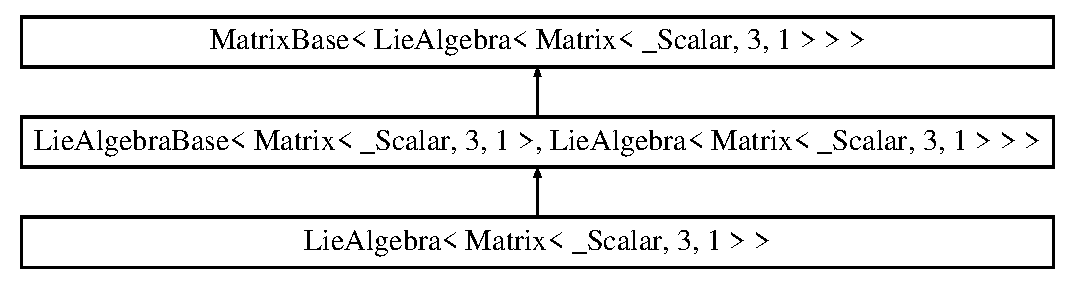
\includegraphics[height=3.000000cm]{class_lie_algebra_3_01_matrix_3_01___scalar_00_013_00_011_01_4_01_4}
\end{center}
\end{figure}
\subsection*{Public Types}
\begin{DoxyCompactItemize}
\item 
typedef internal\+::traits$<$ \hyperlink{class_lie_algebra}{Lie\+Algebra}$<$ Matrix$<$ Scalar, 3, 1 $>$ $>$ $>$\+::\hyperlink{class_lie_algebra_3_01_matrix_3_01___scalar_00_013_00_011_01_4_01_4_a028504a0d794d492dc47b2edd056fe47}{Coefficients} \hyperlink{class_lie_algebra_3_01_matrix_3_01___scalar_00_013_00_011_01_4_01_4_a028504a0d794d492dc47b2edd056fe47}{Coefficients}
\end{DoxyCompactItemize}
\subsection*{Public Member Functions}
\begin{DoxyCompactItemize}
\item 
\hyperlink{class_lie_algebra_3_01_matrix_3_01___scalar_00_013_00_011_01_4_01_4_a34165d53d90245bdbba7ccc7166fc37c}{Lie\+Algebra} ()
\item 
\hyperlink{class_lie_algebra_3_01_matrix_3_01___scalar_00_013_00_011_01_4_01_4_afb65734495d34082830aad472ef0d7cf}{Lie\+Algebra} (const \hyperlink{class_lie_algebra}{Lie\+Algebra} \&a)
\item 
{\footnotesize template$<$class Derived $>$ }\\\hyperlink{class_lie_algebra_3_01_matrix_3_01___scalar_00_013_00_011_01_4_01_4_aff1a3dbf146507fa37d80e11acf095e9}{Lie\+Algebra} (const \hyperlink{class_lie_algebra_base}{Lie\+Algebra\+Base}$<$ typename \hyperlink{class_lie_algebra_base_ae7884e2973ffa35f8b209b2831a066a1}{Base\+::\+Base\+Type}, Derived $>$ \&a)
\item 
\hyperlink{class_lie_algebra_3_01_matrix_3_01___scalar_00_013_00_011_01_4_01_4_af105615d1bcc3d5518841493983ee453}{Lie\+Algebra} (const \hyperlink{class_lie_algebra_3_01_matrix_3_01___scalar_00_013_00_011_01_4_01_4_a028504a0d794d492dc47b2edd056fe47}{Coefficients} \&a)
\item 
\hyperlink{class_lie_algebra_3_01_matrix_3_01___scalar_00_013_00_011_01_4_01_4_a3407ec51785ed5f605f4e56f6fd6df1c}{Lie\+Algebra} (Scalar x, Scalar y, Scalar z)
\item 
\hyperlink{class_lie_algebra_3_01_matrix_3_01___scalar_00_013_00_011_01_4_01_4_a028504a0d794d492dc47b2edd056fe47}{Coefficients} \& \hyperlink{class_lie_algebra_3_01_matrix_3_01___scalar_00_013_00_011_01_4_01_4_a66629af289d8232ba9c2650456654091}{get} ()
\item 
const \hyperlink{class_lie_algebra_3_01_matrix_3_01___scalar_00_013_00_011_01_4_01_4_a028504a0d794d492dc47b2edd056fe47}{Coefficients} \& \hyperlink{class_lie_algebra_3_01_matrix_3_01___scalar_00_013_00_011_01_4_01_4_ad1a20c6cdfc1a3f27ac55685b91611e9}{get} () const
\end{DoxyCompactItemize}
\subsection*{Protected Types}
\begin{DoxyCompactItemize}
\item 
typedef \hyperlink{class_lie_algebra_base}{Lie\+Algebra\+Base}$<$ Matrix$<$ \+\_\+\+Scalar, 3, 1 $>$, \hyperlink{class_lie_algebra}{Lie\+Algebra}$<$ Matrix$<$ \+\_\+\+Scalar, 3, 1 $>$ $>$ $>$ \hyperlink{class_lie_algebra_3_01_matrix_3_01___scalar_00_013_00_011_01_4_01_4_a4ebe70151a0dade8c902424f217a3451}{Base}
\end{DoxyCompactItemize}
\subsection*{Protected Attributes}
\begin{DoxyCompactItemize}
\item 
\hyperlink{class_lie_algebra_3_01_matrix_3_01___scalar_00_013_00_011_01_4_01_4_a028504a0d794d492dc47b2edd056fe47}{Coefficients} \hyperlink{class_lie_algebra_3_01_matrix_3_01___scalar_00_013_00_011_01_4_01_4_aeb9883398abbe97d15ce250f5cb214ce}{m\+\_\+coeffs}
\end{DoxyCompactItemize}


\subsection{Detailed Description}
\subsubsection*{template$<$typename \+\_\+\+Scalar$>$\newline
class Lie\+Algebra$<$ Matrix$<$ \+\_\+\+Scalar, 3, 1 $>$ $>$}



Definition at line 324 of file Lie\+Algebra\+\_\+so3.\+h.



\subsection{Member Typedef Documentation}
\hypertarget{class_lie_algebra_3_01_matrix_3_01___scalar_00_013_00_011_01_4_01_4_a4ebe70151a0dade8c902424f217a3451}{}\label{class_lie_algebra_3_01_matrix_3_01___scalar_00_013_00_011_01_4_01_4_a4ebe70151a0dade8c902424f217a3451} 
\index{Lie\+Algebra$<$ Matrix$<$ \+\_\+\+Scalar, 3, 1 $>$ $>$@{Lie\+Algebra$<$ Matrix$<$ \+\_\+\+Scalar, 3, 1 $>$ $>$}!Base@{Base}}
\index{Base@{Base}!Lie\+Algebra$<$ Matrix$<$ \+\_\+\+Scalar, 3, 1 $>$ $>$@{Lie\+Algebra$<$ Matrix$<$ \+\_\+\+Scalar, 3, 1 $>$ $>$}}
\subsubsection{\texorpdfstring{Base}{Base}}
{\footnotesize\ttfamily template$<$typename \+\_\+\+Scalar $>$ \\
typedef \hyperlink{class_lie_algebra_base}{Lie\+Algebra\+Base}$<$Matrix$<$\+\_\+\+Scalar, 3, 1$>$, \hyperlink{class_lie_algebra}{Lie\+Algebra}$<$Matrix$<$\+\_\+\+Scalar, 3, 1$>$ $>$ $>$ \hyperlink{class_lie_algebra}{Lie\+Algebra}$<$ Matrix$<$ \+\_\+\+Scalar, 3, 1 $>$ $>$\+::\hyperlink{class_lie_algebra_3_01_matrix_3_01___scalar_00_013_00_011_01_4_01_4_a4ebe70151a0dade8c902424f217a3451}{Base}\hspace{0.3cm}{\ttfamily [protected]}}

The inherited class 

Definition at line 329 of file Lie\+Algebra\+\_\+so3.\+h.

\hypertarget{class_lie_algebra_3_01_matrix_3_01___scalar_00_013_00_011_01_4_01_4_a028504a0d794d492dc47b2edd056fe47}{}\label{class_lie_algebra_3_01_matrix_3_01___scalar_00_013_00_011_01_4_01_4_a028504a0d794d492dc47b2edd056fe47} 
\index{Lie\+Algebra$<$ Matrix$<$ \+\_\+\+Scalar, 3, 1 $>$ $>$@{Lie\+Algebra$<$ Matrix$<$ \+\_\+\+Scalar, 3, 1 $>$ $>$}!Coefficients@{Coefficients}}
\index{Coefficients@{Coefficients}!Lie\+Algebra$<$ Matrix$<$ \+\_\+\+Scalar, 3, 1 $>$ $>$@{Lie\+Algebra$<$ Matrix$<$ \+\_\+\+Scalar, 3, 1 $>$ $>$}}
\subsubsection{\texorpdfstring{Coefficients}{Coefficients}}
{\footnotesize\ttfamily template$<$typename \+\_\+\+Scalar $>$ \\
typedef internal\+::traits$<$\hyperlink{class_lie_algebra}{Lie\+Algebra}$<$Matrix$<$Scalar, 3, 1$>$ $>$ $>$\+::\hyperlink{class_lie_algebra_3_01_matrix_3_01___scalar_00_013_00_011_01_4_01_4_a028504a0d794d492dc47b2edd056fe47}{Coefficients} \hyperlink{class_lie_algebra}{Lie\+Algebra}$<$ Matrix$<$ \+\_\+\+Scalar, 3, 1 $>$ $>$\+::\hyperlink{class_lie_algebra_3_01_matrix_3_01___scalar_00_013_00_011_01_4_01_4_a028504a0d794d492dc47b2edd056fe47}{Coefficients}}

The stored coefficients 

Definition at line 337 of file Lie\+Algebra\+\_\+so3.\+h.



\subsection{Constructor \& Destructor Documentation}
\hypertarget{class_lie_algebra_3_01_matrix_3_01___scalar_00_013_00_011_01_4_01_4_a34165d53d90245bdbba7ccc7166fc37c}{}\label{class_lie_algebra_3_01_matrix_3_01___scalar_00_013_00_011_01_4_01_4_a34165d53d90245bdbba7ccc7166fc37c} 
\index{Lie\+Algebra$<$ Matrix$<$ \+\_\+\+Scalar, 3, 1 $>$ $>$@{Lie\+Algebra$<$ Matrix$<$ \+\_\+\+Scalar, 3, 1 $>$ $>$}!Lie\+Algebra@{Lie\+Algebra}}
\index{Lie\+Algebra@{Lie\+Algebra}!Lie\+Algebra$<$ Matrix$<$ \+\_\+\+Scalar, 3, 1 $>$ $>$@{Lie\+Algebra$<$ Matrix$<$ \+\_\+\+Scalar, 3, 1 $>$ $>$}}
\subsubsection{\texorpdfstring{Lie\+Algebra()}{LieAlgebra()}\hspace{0.1cm}{\footnotesize\ttfamily [1/5]}}
{\footnotesize\ttfamily template$<$typename \+\_\+\+Scalar $>$ \\
\hyperlink{class_lie_algebra}{Lie\+Algebra}$<$ Matrix$<$ \+\_\+\+Scalar, 3, 1 $>$ $>$\+::\hyperlink{class_lie_algebra}{Lie\+Algebra} (\begin{DoxyParamCaption}{ }\end{DoxyParamCaption})\hspace{0.3cm}{\ttfamily [inline]}}

Default constructor 

Definition at line 340 of file Lie\+Algebra\+\_\+so3.\+h.

\hypertarget{class_lie_algebra_3_01_matrix_3_01___scalar_00_013_00_011_01_4_01_4_afb65734495d34082830aad472ef0d7cf}{}\label{class_lie_algebra_3_01_matrix_3_01___scalar_00_013_00_011_01_4_01_4_afb65734495d34082830aad472ef0d7cf} 
\index{Lie\+Algebra$<$ Matrix$<$ \+\_\+\+Scalar, 3, 1 $>$ $>$@{Lie\+Algebra$<$ Matrix$<$ \+\_\+\+Scalar, 3, 1 $>$ $>$}!Lie\+Algebra@{Lie\+Algebra}}
\index{Lie\+Algebra@{Lie\+Algebra}!Lie\+Algebra$<$ Matrix$<$ \+\_\+\+Scalar, 3, 1 $>$ $>$@{Lie\+Algebra$<$ Matrix$<$ \+\_\+\+Scalar, 3, 1 $>$ $>$}}
\subsubsection{\texorpdfstring{Lie\+Algebra()}{LieAlgebra()}\hspace{0.1cm}{\footnotesize\ttfamily [2/5]}}
{\footnotesize\ttfamily template$<$typename \+\_\+\+Scalar $>$ \\
\hyperlink{class_lie_algebra}{Lie\+Algebra}$<$ Matrix$<$ \+\_\+\+Scalar, 3, 1 $>$ $>$\+::\hyperlink{class_lie_algebra}{Lie\+Algebra} (\begin{DoxyParamCaption}\item[{const \hyperlink{class_lie_algebra}{Lie\+Algebra}$<$ Matrix$<$ \+\_\+\+Scalar, 3, 1 $>$ $>$ \&}]{a }\end{DoxyParamCaption})\hspace{0.3cm}{\ttfamily [inline]}}

Copy constructor 

Definition at line 342 of file Lie\+Algebra\+\_\+so3.\+h.

\hypertarget{class_lie_algebra_3_01_matrix_3_01___scalar_00_013_00_011_01_4_01_4_aff1a3dbf146507fa37d80e11acf095e9}{}\label{class_lie_algebra_3_01_matrix_3_01___scalar_00_013_00_011_01_4_01_4_aff1a3dbf146507fa37d80e11acf095e9} 
\index{Lie\+Algebra$<$ Matrix$<$ \+\_\+\+Scalar, 3, 1 $>$ $>$@{Lie\+Algebra$<$ Matrix$<$ \+\_\+\+Scalar, 3, 1 $>$ $>$}!Lie\+Algebra@{Lie\+Algebra}}
\index{Lie\+Algebra@{Lie\+Algebra}!Lie\+Algebra$<$ Matrix$<$ \+\_\+\+Scalar, 3, 1 $>$ $>$@{Lie\+Algebra$<$ Matrix$<$ \+\_\+\+Scalar, 3, 1 $>$ $>$}}
\subsubsection{\texorpdfstring{Lie\+Algebra()}{LieAlgebra()}\hspace{0.1cm}{\footnotesize\ttfamily [3/5]}}
{\footnotesize\ttfamily template$<$typename \+\_\+\+Scalar $>$ \\
template$<$class Derived $>$ \\
\hyperlink{class_lie_algebra}{Lie\+Algebra}$<$ Matrix$<$ \+\_\+\+Scalar, 3, 1 $>$ $>$\+::\hyperlink{class_lie_algebra}{Lie\+Algebra} (\begin{DoxyParamCaption}\item[{const \hyperlink{class_lie_algebra_base}{Lie\+Algebra\+Base}$<$ typename \hyperlink{class_lie_algebra_base_ae7884e2973ffa35f8b209b2831a066a1}{Base\+::\+Base\+Type}, Derived $>$ \&}]{a }\end{DoxyParamCaption})\hspace{0.3cm}{\ttfamily [inline]}}

Copy constructor 

Definition at line 345 of file Lie\+Algebra\+\_\+so3.\+h.

\hypertarget{class_lie_algebra_3_01_matrix_3_01___scalar_00_013_00_011_01_4_01_4_af105615d1bcc3d5518841493983ee453}{}\label{class_lie_algebra_3_01_matrix_3_01___scalar_00_013_00_011_01_4_01_4_af105615d1bcc3d5518841493983ee453} 
\index{Lie\+Algebra$<$ Matrix$<$ \+\_\+\+Scalar, 3, 1 $>$ $>$@{Lie\+Algebra$<$ Matrix$<$ \+\_\+\+Scalar, 3, 1 $>$ $>$}!Lie\+Algebra@{Lie\+Algebra}}
\index{Lie\+Algebra@{Lie\+Algebra}!Lie\+Algebra$<$ Matrix$<$ \+\_\+\+Scalar, 3, 1 $>$ $>$@{Lie\+Algebra$<$ Matrix$<$ \+\_\+\+Scalar, 3, 1 $>$ $>$}}
\subsubsection{\texorpdfstring{Lie\+Algebra()}{LieAlgebra()}\hspace{0.1cm}{\footnotesize\ttfamily [4/5]}}
{\footnotesize\ttfamily template$<$typename \+\_\+\+Scalar $>$ \\
\hyperlink{class_lie_algebra}{Lie\+Algebra}$<$ Matrix$<$ \+\_\+\+Scalar, 3, 1 $>$ $>$\+::\hyperlink{class_lie_algebra}{Lie\+Algebra} (\begin{DoxyParamCaption}\item[{const \hyperlink{class_lie_algebra_3_01_matrix_3_01___scalar_00_013_00_011_01_4_01_4_a028504a0d794d492dc47b2edd056fe47}{Coefficients} \&}]{a }\end{DoxyParamCaption})\hspace{0.3cm}{\ttfamily [inline]}}

Copy constructor 

Definition at line 347 of file Lie\+Algebra\+\_\+so3.\+h.

\hypertarget{class_lie_algebra_3_01_matrix_3_01___scalar_00_013_00_011_01_4_01_4_a3407ec51785ed5f605f4e56f6fd6df1c}{}\label{class_lie_algebra_3_01_matrix_3_01___scalar_00_013_00_011_01_4_01_4_a3407ec51785ed5f605f4e56f6fd6df1c} 
\index{Lie\+Algebra$<$ Matrix$<$ \+\_\+\+Scalar, 3, 1 $>$ $>$@{Lie\+Algebra$<$ Matrix$<$ \+\_\+\+Scalar, 3, 1 $>$ $>$}!Lie\+Algebra@{Lie\+Algebra}}
\index{Lie\+Algebra@{Lie\+Algebra}!Lie\+Algebra$<$ Matrix$<$ \+\_\+\+Scalar, 3, 1 $>$ $>$@{Lie\+Algebra$<$ Matrix$<$ \+\_\+\+Scalar, 3, 1 $>$ $>$}}
\subsubsection{\texorpdfstring{Lie\+Algebra()}{LieAlgebra()}\hspace{0.1cm}{\footnotesize\ttfamily [5/5]}}
{\footnotesize\ttfamily template$<$typename \+\_\+\+Scalar $>$ \\
\hyperlink{class_lie_algebra}{Lie\+Algebra}$<$ Matrix$<$ \+\_\+\+Scalar, 3, 1 $>$ $>$\+::\hyperlink{class_lie_algebra}{Lie\+Algebra} (\begin{DoxyParamCaption}\item[{Scalar}]{x,  }\item[{Scalar}]{y,  }\item[{Scalar}]{z }\end{DoxyParamCaption})\hspace{0.3cm}{\ttfamily [inline]}}

Constructs an element of so(3) from 3 scalar {\ttfamily x} {\ttfamily y} {\ttfamily z} 

Definition at line 349 of file Lie\+Algebra\+\_\+so3.\+h.



\subsection{Member Function Documentation}
\hypertarget{class_lie_algebra_3_01_matrix_3_01___scalar_00_013_00_011_01_4_01_4_a66629af289d8232ba9c2650456654091}{}\label{class_lie_algebra_3_01_matrix_3_01___scalar_00_013_00_011_01_4_01_4_a66629af289d8232ba9c2650456654091} 
\index{Lie\+Algebra$<$ Matrix$<$ \+\_\+\+Scalar, 3, 1 $>$ $>$@{Lie\+Algebra$<$ Matrix$<$ \+\_\+\+Scalar, 3, 1 $>$ $>$}!get@{get}}
\index{get@{get}!Lie\+Algebra$<$ Matrix$<$ \+\_\+\+Scalar, 3, 1 $>$ $>$@{Lie\+Algebra$<$ Matrix$<$ \+\_\+\+Scalar, 3, 1 $>$ $>$}}
\subsubsection{\texorpdfstring{get()}{get()}\hspace{0.1cm}{\footnotesize\ttfamily [1/2]}}
{\footnotesize\ttfamily template$<$typename \+\_\+\+Scalar $>$ \\
\hyperlink{class_lie_algebra_3_01_matrix_3_01___scalar_00_013_00_011_01_4_01_4_a028504a0d794d492dc47b2edd056fe47}{Coefficients}\& \hyperlink{class_lie_algebra}{Lie\+Algebra}$<$ Matrix$<$ \+\_\+\+Scalar, 3, 1 $>$ $>$\+::get (\begin{DoxyParamCaption}{ }\end{DoxyParamCaption})\hspace{0.3cm}{\ttfamily [inline]}}

\begin{DoxyReturn}{Returns}
The stored coefficients 
\end{DoxyReturn}


Definition at line 352 of file Lie\+Algebra\+\_\+so3.\+h.

\hypertarget{class_lie_algebra_3_01_matrix_3_01___scalar_00_013_00_011_01_4_01_4_ad1a20c6cdfc1a3f27ac55685b91611e9}{}\label{class_lie_algebra_3_01_matrix_3_01___scalar_00_013_00_011_01_4_01_4_ad1a20c6cdfc1a3f27ac55685b91611e9} 
\index{Lie\+Algebra$<$ Matrix$<$ \+\_\+\+Scalar, 3, 1 $>$ $>$@{Lie\+Algebra$<$ Matrix$<$ \+\_\+\+Scalar, 3, 1 $>$ $>$}!get@{get}}
\index{get@{get}!Lie\+Algebra$<$ Matrix$<$ \+\_\+\+Scalar, 3, 1 $>$ $>$@{Lie\+Algebra$<$ Matrix$<$ \+\_\+\+Scalar, 3, 1 $>$ $>$}}
\subsubsection{\texorpdfstring{get()}{get()}\hspace{0.1cm}{\footnotesize\ttfamily [2/2]}}
{\footnotesize\ttfamily template$<$typename \+\_\+\+Scalar $>$ \\
const \hyperlink{class_lie_algebra_3_01_matrix_3_01___scalar_00_013_00_011_01_4_01_4_a028504a0d794d492dc47b2edd056fe47}{Coefficients}\& \hyperlink{class_lie_algebra}{Lie\+Algebra}$<$ Matrix$<$ \+\_\+\+Scalar, 3, 1 $>$ $>$\+::get (\begin{DoxyParamCaption}{ }\end{DoxyParamCaption}) const\hspace{0.3cm}{\ttfamily [inline]}}

\begin{DoxyReturn}{Returns}
The read-\/only access to the stored coefficients 
\end{DoxyReturn}


Definition at line 354 of file Lie\+Algebra\+\_\+so3.\+h.



\subsection{Member Data Documentation}
\hypertarget{class_lie_algebra_3_01_matrix_3_01___scalar_00_013_00_011_01_4_01_4_aeb9883398abbe97d15ce250f5cb214ce}{}\label{class_lie_algebra_3_01_matrix_3_01___scalar_00_013_00_011_01_4_01_4_aeb9883398abbe97d15ce250f5cb214ce} 
\index{Lie\+Algebra$<$ Matrix$<$ \+\_\+\+Scalar, 3, 1 $>$ $>$@{Lie\+Algebra$<$ Matrix$<$ \+\_\+\+Scalar, 3, 1 $>$ $>$}!m\+\_\+coeffs@{m\+\_\+coeffs}}
\index{m\+\_\+coeffs@{m\+\_\+coeffs}!Lie\+Algebra$<$ Matrix$<$ \+\_\+\+Scalar, 3, 1 $>$ $>$@{Lie\+Algebra$<$ Matrix$<$ \+\_\+\+Scalar, 3, 1 $>$ $>$}}
\subsubsection{\texorpdfstring{m\+\_\+coeffs}{m\_coeffs}}
{\footnotesize\ttfamily template$<$typename \+\_\+\+Scalar $>$ \\
\hyperlink{class_lie_algebra_3_01_matrix_3_01___scalar_00_013_00_011_01_4_01_4_a028504a0d794d492dc47b2edd056fe47}{Coefficients} \hyperlink{class_lie_algebra}{Lie\+Algebra}$<$ Matrix$<$ \+\_\+\+Scalar, 3, 1 $>$ $>$\+::m\+\_\+coeffs\hspace{0.3cm}{\ttfamily [protected]}}

The wrapped coefficients 

Definition at line 358 of file Lie\+Algebra\+\_\+so3.\+h.



The documentation for this class was generated from the following file\+:\begin{DoxyCompactItemize}
\item 
/\+Users/\+Ryan/\+Code/codyco-\/superbuild/libraries/\+Eigen\+Lgsm/unsupported/\+Eigen/src/\+Lgsm/\hyperlink{_lie_algebra__so3_8h}{Lie\+Algebra\+\_\+so3.\+h}\end{DoxyCompactItemize}

\hypertarget{class_lie_algebra_3_01_matrix_3_01___scalar_00_016_00_011_01_4_01_4}{}\section{Lie\+Algebra$<$ Matrix$<$ \+\_\+\+Scalar, 6, 1 $>$ $>$ Class Template Reference}
\label{class_lie_algebra_3_01_matrix_3_01___scalar_00_016_00_011_01_4_01_4}\index{Lie\+Algebra$<$ Matrix$<$ \+\_\+\+Scalar, 6, 1 $>$ $>$@{Lie\+Algebra$<$ Matrix$<$ \+\_\+\+Scalar, 6, 1 $>$ $>$}}


{\ttfamily \#include $<$Lie\+Algebra\+\_\+se3.\+h$>$}

Inheritance diagram for Lie\+Algebra$<$ Matrix$<$ \+\_\+\+Scalar, 6, 1 $>$ $>$\+:\begin{figure}[H]
\begin{center}
\leavevmode
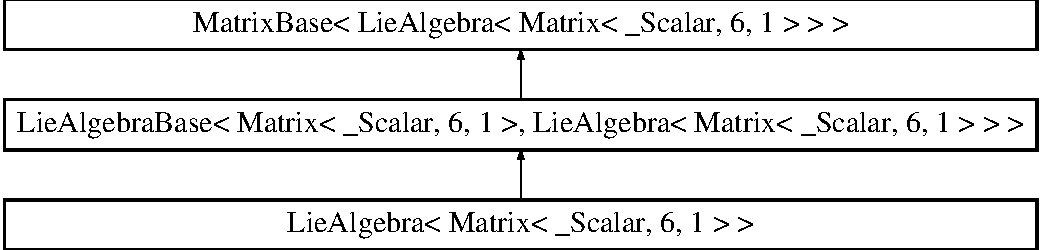
\includegraphics[height=3.000000cm]{class_lie_algebra_3_01_matrix_3_01___scalar_00_016_00_011_01_4_01_4}
\end{center}
\end{figure}
\subsection*{Public Types}
\begin{DoxyCompactItemize}
\item 
typedef \hyperlink{class_lie_algebra_base_ae7884e2973ffa35f8b209b2831a066a1}{Base\+::\+Base\+Type} \hyperlink{class_lie_algebra_3_01_matrix_3_01___scalar_00_016_00_011_01_4_01_4_aa86c8317cea5955c8ba9d0871791ea23}{Base\+Type}
\item 
typedef internal\+::traits$<$ \hyperlink{class_lie_algebra}{Lie\+Algebra}$<$ Matrix$<$ Scalar, 6, 1 $>$ $>$ $>$\+::\hyperlink{class_lie_algebra_3_01_matrix_3_01___scalar_00_016_00_011_01_4_01_4_a2eb9bb9a54a2c7ce0b75b46814ea390e}{Coefficients} \hyperlink{class_lie_algebra_3_01_matrix_3_01___scalar_00_016_00_011_01_4_01_4_a2eb9bb9a54a2c7ce0b75b46814ea390e}{Coefficients}
\end{DoxyCompactItemize}
\subsection*{Public Member Functions}
\begin{DoxyCompactItemize}
\item 
\hyperlink{class_lie_algebra_3_01_matrix_3_01___scalar_00_016_00_011_01_4_01_4_af4f9e777a6752e4a529a8c99f34ab1a3}{Lie\+Algebra} ()
\item 
\hyperlink{class_lie_algebra_3_01_matrix_3_01___scalar_00_016_00_011_01_4_01_4_a3cc3d14a1f6ab78924c3de2d8792d317}{Lie\+Algebra} (const \hyperlink{class_lie_algebra}{Lie\+Algebra} \&g)
\item 
\hyperlink{class_lie_algebra_3_01_matrix_3_01___scalar_00_016_00_011_01_4_01_4_a35c12d04b74c92281c1f8c35fed0701f}{Lie\+Algebra} (const \hyperlink{class_lie_algebra_3_01_matrix_3_01___scalar_00_016_00_011_01_4_01_4_aa86c8317cea5955c8ba9d0871791ea23}{Base\+Type} \&g)
\item 
\hyperlink{class_lie_algebra_3_01_matrix_3_01___scalar_00_016_00_011_01_4_01_4_a83f40c9ea2a210aca42f148397ad2074}{Lie\+Algebra} (Scalar rx, Scalar ry, Scalar rz, Scalar vx, Scalar vy, Scalar vz)
\item 
\hyperlink{class_lie_algebra_3_01_matrix_3_01___scalar_00_016_00_011_01_4_01_4_a9cb95236184bdf617027d9c71fcbf66a}{Lie\+Algebra} (const typename Base\+::so3\+Element \&r, const typename Base\+::\+Vector3 \&v)
\item 
\hyperlink{class_lie_algebra_3_01_matrix_3_01___scalar_00_016_00_011_01_4_01_4_a2eb9bb9a54a2c7ce0b75b46814ea390e}{Coefficients} \& \hyperlink{class_lie_algebra_3_01_matrix_3_01___scalar_00_016_00_011_01_4_01_4_aab00bfaad297d5857dc63fd84c5eed39}{get} ()
\item 
const \hyperlink{class_lie_algebra_3_01_matrix_3_01___scalar_00_016_00_011_01_4_01_4_a2eb9bb9a54a2c7ce0b75b46814ea390e}{Coefficients} \& \hyperlink{class_lie_algebra_3_01_matrix_3_01___scalar_00_016_00_011_01_4_01_4_a8bc6089b5724706b3b3ae5a52dad7c30}{get} () const
\end{DoxyCompactItemize}
\subsection*{Protected Types}
\begin{DoxyCompactItemize}
\item 
typedef \hyperlink{class_lie_algebra_base}{Lie\+Algebra\+Base}$<$ Matrix$<$ \+\_\+\+Scalar, 6, 1 $>$, \hyperlink{class_lie_algebra}{Lie\+Algebra}$<$ Matrix$<$ \+\_\+\+Scalar, 6, 1 $>$ $>$ $>$ \hyperlink{class_lie_algebra_3_01_matrix_3_01___scalar_00_016_00_011_01_4_01_4_a864bf965fc88e54b2f8ff1e7dda63c66}{Base}
\end{DoxyCompactItemize}
\subsection*{Protected Attributes}
\begin{DoxyCompactItemize}
\item 
\hyperlink{class_lie_algebra_3_01_matrix_3_01___scalar_00_016_00_011_01_4_01_4_a2eb9bb9a54a2c7ce0b75b46814ea390e}{Coefficients} \hyperlink{class_lie_algebra_3_01_matrix_3_01___scalar_00_016_00_011_01_4_01_4_ae8bf705677cc037b0f98ca402025389f}{m\+\_\+coeffs}
\end{DoxyCompactItemize}


\subsection{Detailed Description}
\subsubsection*{template$<$typename \+\_\+\+Scalar$>$\newline
class Lie\+Algebra$<$ Matrix$<$ \+\_\+\+Scalar, 6, 1 $>$ $>$}



Definition at line 265 of file Lie\+Algebra\+\_\+se3.\+h.



\subsection{Member Typedef Documentation}
\hypertarget{class_lie_algebra_3_01_matrix_3_01___scalar_00_016_00_011_01_4_01_4_a864bf965fc88e54b2f8ff1e7dda63c66}{}\label{class_lie_algebra_3_01_matrix_3_01___scalar_00_016_00_011_01_4_01_4_a864bf965fc88e54b2f8ff1e7dda63c66} 
\index{Lie\+Algebra$<$ Matrix$<$ \+\_\+\+Scalar, 6, 1 $>$ $>$@{Lie\+Algebra$<$ Matrix$<$ \+\_\+\+Scalar, 6, 1 $>$ $>$}!Base@{Base}}
\index{Base@{Base}!Lie\+Algebra$<$ Matrix$<$ \+\_\+\+Scalar, 6, 1 $>$ $>$@{Lie\+Algebra$<$ Matrix$<$ \+\_\+\+Scalar, 6, 1 $>$ $>$}}
\subsubsection{\texorpdfstring{Base}{Base}}
{\footnotesize\ttfamily template$<$typename \+\_\+\+Scalar $>$ \\
typedef \hyperlink{class_lie_algebra_base}{Lie\+Algebra\+Base}$<$Matrix$<$\+\_\+\+Scalar, 6, 1$>$, \hyperlink{class_lie_algebra}{Lie\+Algebra}$<$Matrix$<$\+\_\+\+Scalar, 6, 1$>$ $>$ $>$ \hyperlink{class_lie_algebra}{Lie\+Algebra}$<$ Matrix$<$ \+\_\+\+Scalar, 6, 1 $>$ $>$\+::\hyperlink{class_lie_algebra_3_01_matrix_3_01___scalar_00_016_00_011_01_4_01_4_a864bf965fc88e54b2f8ff1e7dda63c66}{Base}\hspace{0.3cm}{\ttfamily [protected]}}

The inherited class 

Definition at line 270 of file Lie\+Algebra\+\_\+se3.\+h.

\hypertarget{class_lie_algebra_3_01_matrix_3_01___scalar_00_016_00_011_01_4_01_4_aa86c8317cea5955c8ba9d0871791ea23}{}\label{class_lie_algebra_3_01_matrix_3_01___scalar_00_016_00_011_01_4_01_4_aa86c8317cea5955c8ba9d0871791ea23} 
\index{Lie\+Algebra$<$ Matrix$<$ \+\_\+\+Scalar, 6, 1 $>$ $>$@{Lie\+Algebra$<$ Matrix$<$ \+\_\+\+Scalar, 6, 1 $>$ $>$}!Base\+Type@{Base\+Type}}
\index{Base\+Type@{Base\+Type}!Lie\+Algebra$<$ Matrix$<$ \+\_\+\+Scalar, 6, 1 $>$ $>$@{Lie\+Algebra$<$ Matrix$<$ \+\_\+\+Scalar, 6, 1 $>$ $>$}}
\subsubsection{\texorpdfstring{Base\+Type}{BaseType}}
{\footnotesize\ttfamily template$<$typename \+\_\+\+Scalar $>$ \\
typedef \hyperlink{class_lie_algebra_base_ae7884e2973ffa35f8b209b2831a066a1}{Base\+::\+Base\+Type} \hyperlink{class_lie_algebra}{Lie\+Algebra}$<$ Matrix$<$ \+\_\+\+Scalar, 6, 1 $>$ $>$\+::\hyperlink{class_lie_algebra_3_01_matrix_3_01___scalar_00_016_00_011_01_4_01_4_aa86c8317cea5955c8ba9d0871791ea23}{Base\+Type}}

The type of the underlying array 

Definition at line 278 of file Lie\+Algebra\+\_\+se3.\+h.

\hypertarget{class_lie_algebra_3_01_matrix_3_01___scalar_00_016_00_011_01_4_01_4_a2eb9bb9a54a2c7ce0b75b46814ea390e}{}\label{class_lie_algebra_3_01_matrix_3_01___scalar_00_016_00_011_01_4_01_4_a2eb9bb9a54a2c7ce0b75b46814ea390e} 
\index{Lie\+Algebra$<$ Matrix$<$ \+\_\+\+Scalar, 6, 1 $>$ $>$@{Lie\+Algebra$<$ Matrix$<$ \+\_\+\+Scalar, 6, 1 $>$ $>$}!Coefficients@{Coefficients}}
\index{Coefficients@{Coefficients}!Lie\+Algebra$<$ Matrix$<$ \+\_\+\+Scalar, 6, 1 $>$ $>$@{Lie\+Algebra$<$ Matrix$<$ \+\_\+\+Scalar, 6, 1 $>$ $>$}}
\subsubsection{\texorpdfstring{Coefficients}{Coefficients}}
{\footnotesize\ttfamily template$<$typename \+\_\+\+Scalar $>$ \\
typedef internal\+::traits$<$\hyperlink{class_lie_algebra}{Lie\+Algebra}$<$Matrix$<$Scalar, 6, 1$>$ $>$ $>$\+::\hyperlink{class_lie_algebra_3_01_matrix_3_01___scalar_00_016_00_011_01_4_01_4_a2eb9bb9a54a2c7ce0b75b46814ea390e}{Coefficients} \hyperlink{class_lie_algebra}{Lie\+Algebra}$<$ Matrix$<$ \+\_\+\+Scalar, 6, 1 $>$ $>$\+::\hyperlink{class_lie_algebra_3_01_matrix_3_01___scalar_00_016_00_011_01_4_01_4_a2eb9bb9a54a2c7ce0b75b46814ea390e}{Coefficients}}

The stored coefficients 

Definition at line 280 of file Lie\+Algebra\+\_\+se3.\+h.



\subsection{Constructor \& Destructor Documentation}
\hypertarget{class_lie_algebra_3_01_matrix_3_01___scalar_00_016_00_011_01_4_01_4_af4f9e777a6752e4a529a8c99f34ab1a3}{}\label{class_lie_algebra_3_01_matrix_3_01___scalar_00_016_00_011_01_4_01_4_af4f9e777a6752e4a529a8c99f34ab1a3} 
\index{Lie\+Algebra$<$ Matrix$<$ \+\_\+\+Scalar, 6, 1 $>$ $>$@{Lie\+Algebra$<$ Matrix$<$ \+\_\+\+Scalar, 6, 1 $>$ $>$}!Lie\+Algebra@{Lie\+Algebra}}
\index{Lie\+Algebra@{Lie\+Algebra}!Lie\+Algebra$<$ Matrix$<$ \+\_\+\+Scalar, 6, 1 $>$ $>$@{Lie\+Algebra$<$ Matrix$<$ \+\_\+\+Scalar, 6, 1 $>$ $>$}}
\subsubsection{\texorpdfstring{Lie\+Algebra()}{LieAlgebra()}\hspace{0.1cm}{\footnotesize\ttfamily [1/5]}}
{\footnotesize\ttfamily template$<$typename \+\_\+\+Scalar $>$ \\
\hyperlink{class_lie_algebra}{Lie\+Algebra}$<$ Matrix$<$ \+\_\+\+Scalar, 6, 1 $>$ $>$\+::\hyperlink{class_lie_algebra}{Lie\+Algebra} (\begin{DoxyParamCaption}{ }\end{DoxyParamCaption})\hspace{0.3cm}{\ttfamily [inline]}}

Default constructor 

Definition at line 283 of file Lie\+Algebra\+\_\+se3.\+h.

\hypertarget{class_lie_algebra_3_01_matrix_3_01___scalar_00_016_00_011_01_4_01_4_a3cc3d14a1f6ab78924c3de2d8792d317}{}\label{class_lie_algebra_3_01_matrix_3_01___scalar_00_016_00_011_01_4_01_4_a3cc3d14a1f6ab78924c3de2d8792d317} 
\index{Lie\+Algebra$<$ Matrix$<$ \+\_\+\+Scalar, 6, 1 $>$ $>$@{Lie\+Algebra$<$ Matrix$<$ \+\_\+\+Scalar, 6, 1 $>$ $>$}!Lie\+Algebra@{Lie\+Algebra}}
\index{Lie\+Algebra@{Lie\+Algebra}!Lie\+Algebra$<$ Matrix$<$ \+\_\+\+Scalar, 6, 1 $>$ $>$@{Lie\+Algebra$<$ Matrix$<$ \+\_\+\+Scalar, 6, 1 $>$ $>$}}
\subsubsection{\texorpdfstring{Lie\+Algebra()}{LieAlgebra()}\hspace{0.1cm}{\footnotesize\ttfamily [2/5]}}
{\footnotesize\ttfamily template$<$typename \+\_\+\+Scalar $>$ \\
\hyperlink{class_lie_algebra}{Lie\+Algebra}$<$ Matrix$<$ \+\_\+\+Scalar, 6, 1 $>$ $>$\+::\hyperlink{class_lie_algebra}{Lie\+Algebra} (\begin{DoxyParamCaption}\item[{const \hyperlink{class_lie_algebra}{Lie\+Algebra}$<$ Matrix$<$ \+\_\+\+Scalar, 6, 1 $>$ $>$ \&}]{g }\end{DoxyParamCaption})\hspace{0.3cm}{\ttfamily [inline]}}

Copy constructor 

Definition at line 285 of file Lie\+Algebra\+\_\+se3.\+h.

\hypertarget{class_lie_algebra_3_01_matrix_3_01___scalar_00_016_00_011_01_4_01_4_a35c12d04b74c92281c1f8c35fed0701f}{}\label{class_lie_algebra_3_01_matrix_3_01___scalar_00_016_00_011_01_4_01_4_a35c12d04b74c92281c1f8c35fed0701f} 
\index{Lie\+Algebra$<$ Matrix$<$ \+\_\+\+Scalar, 6, 1 $>$ $>$@{Lie\+Algebra$<$ Matrix$<$ \+\_\+\+Scalar, 6, 1 $>$ $>$}!Lie\+Algebra@{Lie\+Algebra}}
\index{Lie\+Algebra@{Lie\+Algebra}!Lie\+Algebra$<$ Matrix$<$ \+\_\+\+Scalar, 6, 1 $>$ $>$@{Lie\+Algebra$<$ Matrix$<$ \+\_\+\+Scalar, 6, 1 $>$ $>$}}
\subsubsection{\texorpdfstring{Lie\+Algebra()}{LieAlgebra()}\hspace{0.1cm}{\footnotesize\ttfamily [3/5]}}
{\footnotesize\ttfamily template$<$typename \+\_\+\+Scalar $>$ \\
\hyperlink{class_lie_algebra}{Lie\+Algebra}$<$ Matrix$<$ \+\_\+\+Scalar, 6, 1 $>$ $>$\+::\hyperlink{class_lie_algebra}{Lie\+Algebra} (\begin{DoxyParamCaption}\item[{const \hyperlink{class_lie_algebra_3_01_matrix_3_01___scalar_00_016_00_011_01_4_01_4_aa86c8317cea5955c8ba9d0871791ea23}{Base\+Type} \&}]{g }\end{DoxyParamCaption})\hspace{0.3cm}{\ttfamily [inline]}}

Copy constructor 

Definition at line 287 of file Lie\+Algebra\+\_\+se3.\+h.

\hypertarget{class_lie_algebra_3_01_matrix_3_01___scalar_00_016_00_011_01_4_01_4_a83f40c9ea2a210aca42f148397ad2074}{}\label{class_lie_algebra_3_01_matrix_3_01___scalar_00_016_00_011_01_4_01_4_a83f40c9ea2a210aca42f148397ad2074} 
\index{Lie\+Algebra$<$ Matrix$<$ \+\_\+\+Scalar, 6, 1 $>$ $>$@{Lie\+Algebra$<$ Matrix$<$ \+\_\+\+Scalar, 6, 1 $>$ $>$}!Lie\+Algebra@{Lie\+Algebra}}
\index{Lie\+Algebra@{Lie\+Algebra}!Lie\+Algebra$<$ Matrix$<$ \+\_\+\+Scalar, 6, 1 $>$ $>$@{Lie\+Algebra$<$ Matrix$<$ \+\_\+\+Scalar, 6, 1 $>$ $>$}}
\subsubsection{\texorpdfstring{Lie\+Algebra()}{LieAlgebra()}\hspace{0.1cm}{\footnotesize\ttfamily [4/5]}}
{\footnotesize\ttfamily template$<$typename \+\_\+\+Scalar $>$ \\
\hyperlink{class_lie_algebra}{Lie\+Algebra}$<$ Matrix$<$ \+\_\+\+Scalar, 6, 1 $>$ $>$\+::\hyperlink{class_lie_algebra}{Lie\+Algebra} (\begin{DoxyParamCaption}\item[{Scalar}]{rx,  }\item[{Scalar}]{ry,  }\item[{Scalar}]{rz,  }\item[{Scalar}]{vx,  }\item[{Scalar}]{vy,  }\item[{Scalar}]{vz }\end{DoxyParamCaption})\hspace{0.3cm}{\ttfamily [inline]}}

Constructs an element of se(3) from 6 scalar 

Definition at line 289 of file Lie\+Algebra\+\_\+se3.\+h.

\hypertarget{class_lie_algebra_3_01_matrix_3_01___scalar_00_016_00_011_01_4_01_4_a9cb95236184bdf617027d9c71fcbf66a}{}\label{class_lie_algebra_3_01_matrix_3_01___scalar_00_016_00_011_01_4_01_4_a9cb95236184bdf617027d9c71fcbf66a} 
\index{Lie\+Algebra$<$ Matrix$<$ \+\_\+\+Scalar, 6, 1 $>$ $>$@{Lie\+Algebra$<$ Matrix$<$ \+\_\+\+Scalar, 6, 1 $>$ $>$}!Lie\+Algebra@{Lie\+Algebra}}
\index{Lie\+Algebra@{Lie\+Algebra}!Lie\+Algebra$<$ Matrix$<$ \+\_\+\+Scalar, 6, 1 $>$ $>$@{Lie\+Algebra$<$ Matrix$<$ \+\_\+\+Scalar, 6, 1 $>$ $>$}}
\subsubsection{\texorpdfstring{Lie\+Algebra()}{LieAlgebra()}\hspace{0.1cm}{\footnotesize\ttfamily [5/5]}}
{\footnotesize\ttfamily template$<$typename \+\_\+\+Scalar $>$ \\
\hyperlink{class_lie_algebra}{Lie\+Algebra}$<$ Matrix$<$ \+\_\+\+Scalar, 6, 1 $>$ $>$\+::\hyperlink{class_lie_algebra}{Lie\+Algebra} (\begin{DoxyParamCaption}\item[{const typename Base\+::so3\+Element \&}]{r,  }\item[{const typename Base\+::\+Vector3 \&}]{v }\end{DoxyParamCaption})\hspace{0.3cm}{\ttfamily [inline]}}

Constructs a element of se(3) from an element of so(3) {\ttfamily r} and R$^\wedge$3 {\ttfamily v} 

Definition at line 298 of file Lie\+Algebra\+\_\+se3.\+h.



\subsection{Member Function Documentation}
\hypertarget{class_lie_algebra_3_01_matrix_3_01___scalar_00_016_00_011_01_4_01_4_aab00bfaad297d5857dc63fd84c5eed39}{}\label{class_lie_algebra_3_01_matrix_3_01___scalar_00_016_00_011_01_4_01_4_aab00bfaad297d5857dc63fd84c5eed39} 
\index{Lie\+Algebra$<$ Matrix$<$ \+\_\+\+Scalar, 6, 1 $>$ $>$@{Lie\+Algebra$<$ Matrix$<$ \+\_\+\+Scalar, 6, 1 $>$ $>$}!get@{get}}
\index{get@{get}!Lie\+Algebra$<$ Matrix$<$ \+\_\+\+Scalar, 6, 1 $>$ $>$@{Lie\+Algebra$<$ Matrix$<$ \+\_\+\+Scalar, 6, 1 $>$ $>$}}
\subsubsection{\texorpdfstring{get()}{get()}\hspace{0.1cm}{\footnotesize\ttfamily [1/2]}}
{\footnotesize\ttfamily template$<$typename \+\_\+\+Scalar $>$ \\
\hyperlink{class_lie_algebra_3_01_matrix_3_01___scalar_00_016_00_011_01_4_01_4_a2eb9bb9a54a2c7ce0b75b46814ea390e}{Coefficients}\& \hyperlink{class_lie_algebra}{Lie\+Algebra}$<$ Matrix$<$ \+\_\+\+Scalar, 6, 1 $>$ $>$\+::get (\begin{DoxyParamCaption}{ }\end{DoxyParamCaption})\hspace{0.3cm}{\ttfamily [inline]}}

\begin{DoxyReturn}{Returns}
The stored coefficients 
\end{DoxyReturn}


Definition at line 304 of file Lie\+Algebra\+\_\+se3.\+h.

\hypertarget{class_lie_algebra_3_01_matrix_3_01___scalar_00_016_00_011_01_4_01_4_a8bc6089b5724706b3b3ae5a52dad7c30}{}\label{class_lie_algebra_3_01_matrix_3_01___scalar_00_016_00_011_01_4_01_4_a8bc6089b5724706b3b3ae5a52dad7c30} 
\index{Lie\+Algebra$<$ Matrix$<$ \+\_\+\+Scalar, 6, 1 $>$ $>$@{Lie\+Algebra$<$ Matrix$<$ \+\_\+\+Scalar, 6, 1 $>$ $>$}!get@{get}}
\index{get@{get}!Lie\+Algebra$<$ Matrix$<$ \+\_\+\+Scalar, 6, 1 $>$ $>$@{Lie\+Algebra$<$ Matrix$<$ \+\_\+\+Scalar, 6, 1 $>$ $>$}}
\subsubsection{\texorpdfstring{get()}{get()}\hspace{0.1cm}{\footnotesize\ttfamily [2/2]}}
{\footnotesize\ttfamily template$<$typename \+\_\+\+Scalar $>$ \\
const \hyperlink{class_lie_algebra_3_01_matrix_3_01___scalar_00_016_00_011_01_4_01_4_a2eb9bb9a54a2c7ce0b75b46814ea390e}{Coefficients}\& \hyperlink{class_lie_algebra}{Lie\+Algebra}$<$ Matrix$<$ \+\_\+\+Scalar, 6, 1 $>$ $>$\+::get (\begin{DoxyParamCaption}{ }\end{DoxyParamCaption}) const\hspace{0.3cm}{\ttfamily [inline]}}

\begin{DoxyReturn}{Returns}
The read-\/only access to the stored coefficients 
\end{DoxyReturn}


Definition at line 306 of file Lie\+Algebra\+\_\+se3.\+h.



\subsection{Member Data Documentation}
\hypertarget{class_lie_algebra_3_01_matrix_3_01___scalar_00_016_00_011_01_4_01_4_ae8bf705677cc037b0f98ca402025389f}{}\label{class_lie_algebra_3_01_matrix_3_01___scalar_00_016_00_011_01_4_01_4_ae8bf705677cc037b0f98ca402025389f} 
\index{Lie\+Algebra$<$ Matrix$<$ \+\_\+\+Scalar, 6, 1 $>$ $>$@{Lie\+Algebra$<$ Matrix$<$ \+\_\+\+Scalar, 6, 1 $>$ $>$}!m\+\_\+coeffs@{m\+\_\+coeffs}}
\index{m\+\_\+coeffs@{m\+\_\+coeffs}!Lie\+Algebra$<$ Matrix$<$ \+\_\+\+Scalar, 6, 1 $>$ $>$@{Lie\+Algebra$<$ Matrix$<$ \+\_\+\+Scalar, 6, 1 $>$ $>$}}
\subsubsection{\texorpdfstring{m\+\_\+coeffs}{m\_coeffs}}
{\footnotesize\ttfamily template$<$typename \+\_\+\+Scalar $>$ \\
\hyperlink{class_lie_algebra_3_01_matrix_3_01___scalar_00_016_00_011_01_4_01_4_a2eb9bb9a54a2c7ce0b75b46814ea390e}{Coefficients} \hyperlink{class_lie_algebra}{Lie\+Algebra}$<$ Matrix$<$ \+\_\+\+Scalar, 6, 1 $>$ $>$\+::m\+\_\+coeffs\hspace{0.3cm}{\ttfamily [protected]}}

The wrapped coefficients 

Definition at line 310 of file Lie\+Algebra\+\_\+se3.\+h.



The documentation for this class was generated from the following file\+:\begin{DoxyCompactItemize}
\item 
/\+Users/\+Ryan/\+Code/codyco-\/superbuild/libraries/\+Eigen\+Lgsm/unsupported/\+Eigen/src/\+Lgsm/\hyperlink{_lie_algebra__se3_8h}{Lie\+Algebra\+\_\+se3.\+h}\end{DoxyCompactItemize}

\hypertarget{class_lie_algebra_base}{}\section{Lie\+Algebra\+Base$<$ A, Derived $>$ Class Template Reference}
\label{class_lie_algebra_base}\index{Lie\+Algebra\+Base$<$ A, Derived $>$@{Lie\+Algebra\+Base$<$ A, Derived $>$}}


{\ttfamily \#include $<$Lie\+Algebra.\+h$>$}

Inheritance diagram for Lie\+Algebra\+Base$<$ A, Derived $>$\+:\begin{figure}[H]
\begin{center}
\leavevmode
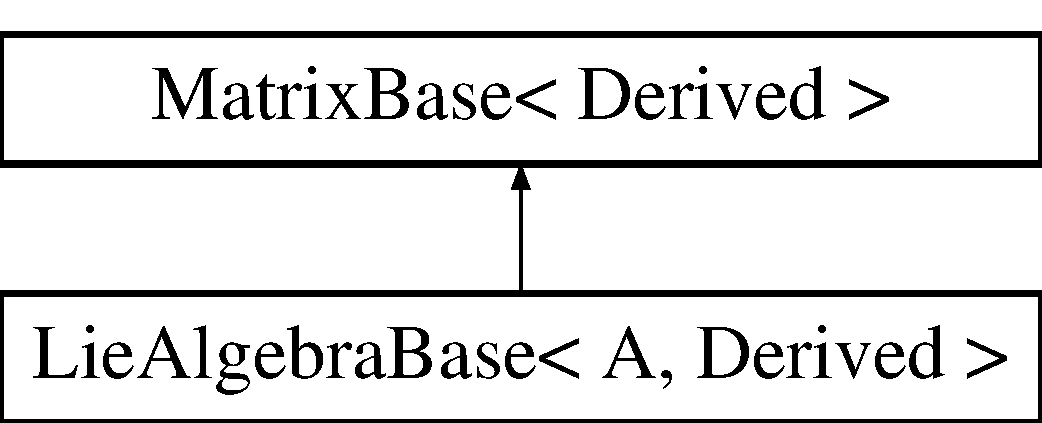
\includegraphics[height=2.000000cm]{class_lie_algebra_base}
\end{center}
\end{figure}
\subsection*{Public Types}
\begin{DoxyCompactItemize}
\item 
typedef A \hyperlink{class_lie_algebra_base_ae7884e2973ffa35f8b209b2831a066a1}{Base\+Type}
\item 
typedef internal\+::traits$<$ Derived $>$\+::\hyperlink{class_lie_algebra_base_a8e61a02d3c5f7a0b4bd87a4ccd47dc9a}{Coefficients} \hyperlink{class_lie_algebra_base_a8e61a02d3c5f7a0b4bd87a4ccd47dc9a}{Coefficients}
\item 
typedef \hyperlink{class_lie_algebra}{Lie\+Algebra}$<$ \hyperlink{class_lie_algebra_base_ae7884e2973ffa35f8b209b2831a066a1}{Base\+Type} $>$ \hyperlink{class_lie_algebra_base_a360d9c7789cab342ccfc3bff779aba6e}{Plain\+Object}
\item 
typedef \hyperlink{class_lie_algebra_dual}{Lie\+Algebra\+Dual}$<$ \hyperlink{class_lie_algebra_base_ae7884e2973ffa35f8b209b2831a066a1}{Base\+Type} $>$ \hyperlink{class_lie_algebra_base_a295c784d24a14e39763f3ff5c2abd155}{Algebra\+Dual}
\item 
typedef Derived\+::\+Lie\+Group \hyperlink{class_lie_algebra_base_aab4a5b7a728102ffe801534c0fc10d79}{Group}
\end{DoxyCompactItemize}
\subsection*{Public Member Functions}
\begin{DoxyCompactItemize}
\item 
{\footnotesize template$<$class Other\+Derived $>$ }\\\hyperlink{class_lie_algebra_base_a360d9c7789cab342ccfc3bff779aba6e}{Plain\+Object} \hyperlink{class_lie_algebra_base_ab7969d13d46f11b7b769b9db48e67267}{bracket} (const \hyperlink{class_lie_algebra_base}{Lie\+Algebra\+Base}$<$ \hyperlink{class_lie_algebra_base_ae7884e2973ffa35f8b209b2831a066a1}{Base\+Type}, Other\+Derived $>$ \&a) const
\item 
{\footnotesize template$<$class Other\+Derived $>$ }\\const \hyperlink{class_lie_algebra_base_a360d9c7789cab342ccfc3bff779aba6e}{Plain\+Object} \hyperlink{class_lie_algebra_base_af1a16f8a8e2fdcb5c1529ffa3e7f2af9}{adjoint} (const \hyperlink{class_lie_algebra_base}{Lie\+Algebra\+Base}$<$ \hyperlink{class_lie_algebra_base_ae7884e2973ffa35f8b209b2831a066a1}{Base\+Type}, Other\+Derived $>$ \&a) const
\item 
\hyperlink{class_lie_algebra_base_aab4a5b7a728102ffe801534c0fc10d79}{Group} \hyperlink{class_lie_algebra_base_aafe7d43a29d43aed54dd91b3a3a4c9f7}{exp} (Scalar precision=1.e-\/6) const
\item 
const Derived \& \hyperlink{class_lie_algebra_base_a2d4fdcb29ba14871036418e90087b16e}{derived} () const
\item 
Derived \& \hyperlink{class_lie_algebra_base_aea14b5c74318541991d64eff30d8b1af}{derived} ()
\item 
\hyperlink{class_lie_algebra_base_a8e61a02d3c5f7a0b4bd87a4ccd47dc9a}{Coefficients} \& \hyperlink{class_lie_algebra_base_ae98f35321a261257a8aeee7d8388df2d}{get} ()
\item 
const \hyperlink{class_lie_algebra_base_a8e61a02d3c5f7a0b4bd87a4ccd47dc9a}{Coefficients} \& \hyperlink{class_lie_algebra_base_aa54c9478545ff1e222217a3bc19ec5d2}{get} () const
\end{DoxyCompactItemize}
\subsection*{Protected Types}
\begin{DoxyCompactItemize}
\item 
typedef Matrix\+Base$<$ Derived $>$ \hyperlink{class_lie_algebra_base_aa2d976fdcf8653f8a5a3f414e725a3e9}{Base}
\end{DoxyCompactItemize}


\subsection{Detailed Description}
\subsubsection*{template$<$class A, class Derived$>$\newline
class Lie\+Algebra\+Base$<$ A, Derived $>$}



Definition at line 34 of file Lie\+Algebra.\+h.



\subsection{Member Typedef Documentation}
\hypertarget{class_lie_algebra_base_a295c784d24a14e39763f3ff5c2abd155}{}\label{class_lie_algebra_base_a295c784d24a14e39763f3ff5c2abd155} 
\index{Lie\+Algebra\+Base@{Lie\+Algebra\+Base}!Algebra\+Dual@{Algebra\+Dual}}
\index{Algebra\+Dual@{Algebra\+Dual}!Lie\+Algebra\+Base@{Lie\+Algebra\+Base}}
\subsubsection{\texorpdfstring{Algebra\+Dual}{AlgebraDual}}
{\footnotesize\ttfamily template$<$class A, class Derived$>$ \\
typedef \hyperlink{class_lie_algebra_dual}{Lie\+Algebra\+Dual}$<$\hyperlink{class_lie_algebra_base_ae7884e2973ffa35f8b209b2831a066a1}{Base\+Type}$>$ \hyperlink{class_lie_algebra_base}{Lie\+Algebra\+Base}$<$ A, Derived $>$\+::\hyperlink{class_lie_algebra_base_a295c784d24a14e39763f3ff5c2abd155}{Algebra\+Dual}}

The type of the dual Algebra 

Definition at line 53 of file Lie\+Algebra.\+h.

\hypertarget{class_lie_algebra_base_aa2d976fdcf8653f8a5a3f414e725a3e9}{}\label{class_lie_algebra_base_aa2d976fdcf8653f8a5a3f414e725a3e9} 
\index{Lie\+Algebra\+Base@{Lie\+Algebra\+Base}!Base@{Base}}
\index{Base@{Base}!Lie\+Algebra\+Base@{Lie\+Algebra\+Base}}
\subsubsection{\texorpdfstring{Base}{Base}}
{\footnotesize\ttfamily template$<$class A, class Derived$>$ \\
typedef Matrix\+Base$<$Derived$>$ \hyperlink{class_lie_algebra_base}{Lie\+Algebra\+Base}$<$ A, Derived $>$\+::\hyperlink{class_lie_algebra_base_aa2d976fdcf8653f8a5a3f414e725a3e9}{Base}\hspace{0.3cm}{\ttfamily [protected]}}

The inherited class 

Definition at line 37 of file Lie\+Algebra.\+h.

\hypertarget{class_lie_algebra_base_ae7884e2973ffa35f8b209b2831a066a1}{}\label{class_lie_algebra_base_ae7884e2973ffa35f8b209b2831a066a1} 
\index{Lie\+Algebra\+Base@{Lie\+Algebra\+Base}!Base\+Type@{Base\+Type}}
\index{Base\+Type@{Base\+Type}!Lie\+Algebra\+Base@{Lie\+Algebra\+Base}}
\subsubsection{\texorpdfstring{Base\+Type}{BaseType}}
{\footnotesize\ttfamily template$<$class A, class Derived$>$ \\
typedef A \hyperlink{class_lie_algebra_base}{Lie\+Algebra\+Base}$<$ A, Derived $>$\+::\hyperlink{class_lie_algebra_base_ae7884e2973ffa35f8b209b2831a066a1}{Base\+Type}}

The wrapped class 

Definition at line 47 of file Lie\+Algebra.\+h.

\hypertarget{class_lie_algebra_base_a8e61a02d3c5f7a0b4bd87a4ccd47dc9a}{}\label{class_lie_algebra_base_a8e61a02d3c5f7a0b4bd87a4ccd47dc9a} 
\index{Lie\+Algebra\+Base@{Lie\+Algebra\+Base}!Coefficients@{Coefficients}}
\index{Coefficients@{Coefficients}!Lie\+Algebra\+Base@{Lie\+Algebra\+Base}}
\subsubsection{\texorpdfstring{Coefficients}{Coefficients}}
{\footnotesize\ttfamily template$<$class A, class Derived$>$ \\
typedef internal\+::traits$<$Derived$>$\+::\hyperlink{class_lie_algebra_base_a8e61a02d3c5f7a0b4bd87a4ccd47dc9a}{Coefficients} \hyperlink{class_lie_algebra_base}{Lie\+Algebra\+Base}$<$ A, Derived $>$\+::\hyperlink{class_lie_algebra_base_a8e61a02d3c5f7a0b4bd87a4ccd47dc9a}{Coefficients}}

The kind of stored coefficients 

Definition at line 49 of file Lie\+Algebra.\+h.

\hypertarget{class_lie_algebra_base_aab4a5b7a728102ffe801534c0fc10d79}{}\label{class_lie_algebra_base_aab4a5b7a728102ffe801534c0fc10d79} 
\index{Lie\+Algebra\+Base@{Lie\+Algebra\+Base}!Group@{Group}}
\index{Group@{Group}!Lie\+Algebra\+Base@{Lie\+Algebra\+Base}}
\subsubsection{\texorpdfstring{Group}{Group}}
{\footnotesize\ttfamily template$<$class A, class Derived$>$ \\
typedef Derived\+::\+Lie\+Group \hyperlink{class_lie_algebra_base}{Lie\+Algebra\+Base}$<$ A, Derived $>$\+::\hyperlink{class_lie_algebra_base_aab4a5b7a728102ffe801534c0fc10d79}{Group}}

The type of the associated Lie Group 

Definition at line 55 of file Lie\+Algebra.\+h.

\hypertarget{class_lie_algebra_base_a360d9c7789cab342ccfc3bff779aba6e}{}\label{class_lie_algebra_base_a360d9c7789cab342ccfc3bff779aba6e} 
\index{Lie\+Algebra\+Base@{Lie\+Algebra\+Base}!Plain\+Object@{Plain\+Object}}
\index{Plain\+Object@{Plain\+Object}!Lie\+Algebra\+Base@{Lie\+Algebra\+Base}}
\subsubsection{\texorpdfstring{Plain\+Object}{PlainObject}}
{\footnotesize\ttfamily template$<$class A, class Derived$>$ \\
typedef \hyperlink{class_lie_algebra}{Lie\+Algebra}$<$\hyperlink{class_lie_algebra_base_ae7884e2973ffa35f8b209b2831a066a1}{Base\+Type}$>$ \hyperlink{class_lie_algebra_base}{Lie\+Algebra\+Base}$<$ A, Derived $>$\+::\hyperlink{class_lie_algebra_base_a360d9c7789cab342ccfc3bff779aba6e}{Plain\+Object}}

The plain object returned, while using Map$<$Lie\+Algebra$<$ $>$ $>$ 

Definition at line 51 of file Lie\+Algebra.\+h.



\subsection{Member Function Documentation}
\hypertarget{class_lie_algebra_base_af1a16f8a8e2fdcb5c1529ffa3e7f2af9}{}\label{class_lie_algebra_base_af1a16f8a8e2fdcb5c1529ffa3e7f2af9} 
\index{Lie\+Algebra\+Base@{Lie\+Algebra\+Base}!adjoint@{adjoint}}
\index{adjoint@{adjoint}!Lie\+Algebra\+Base@{Lie\+Algebra\+Base}}
\subsubsection{\texorpdfstring{adjoint()}{adjoint()}}
{\footnotesize\ttfamily template$<$class A, class Derived$>$ \\
template$<$class Other\+Derived $>$ \\
const \hyperlink{class_lie_algebra_base_a360d9c7789cab342ccfc3bff779aba6e}{Plain\+Object} \hyperlink{class_lie_algebra_base}{Lie\+Algebra\+Base}$<$ A, Derived $>$\+::adjoint (\begin{DoxyParamCaption}\item[{const \hyperlink{class_lie_algebra_base}{Lie\+Algebra\+Base}$<$ \hyperlink{class_lie_algebra_base_ae7884e2973ffa35f8b209b2831a066a1}{Base\+Type}, Other\+Derived $>$ \&}]{a }\end{DoxyParamCaption}) const\hspace{0.3cm}{\ttfamily [inline]}}

Adjoint representation of the Lie Algebra \hypertarget{class_lie_algebra_base_ab7969d13d46f11b7b769b9db48e67267}{}\label{class_lie_algebra_base_ab7969d13d46f11b7b769b9db48e67267} 
\index{Lie\+Algebra\+Base@{Lie\+Algebra\+Base}!bracket@{bracket}}
\index{bracket@{bracket}!Lie\+Algebra\+Base@{Lie\+Algebra\+Base}}
\subsubsection{\texorpdfstring{bracket()}{bracket()}}
{\footnotesize\ttfamily template$<$class A, class Derived$>$ \\
template$<$class Other\+Derived $>$ \\
\hyperlink{class_lie_algebra_base_a360d9c7789cab342ccfc3bff779aba6e}{Plain\+Object} \hyperlink{class_lie_algebra_base}{Lie\+Algebra\+Base}$<$ A, Derived $>$\+::bracket (\begin{DoxyParamCaption}\item[{const \hyperlink{class_lie_algebra_base}{Lie\+Algebra\+Base}$<$ \hyperlink{class_lie_algebra_base_ae7884e2973ffa35f8b209b2831a066a1}{Base\+Type}, Other\+Derived $>$ \&}]{a }\end{DoxyParamCaption}) const\hspace{0.3cm}{\ttfamily [inline]}}

Lie Bracket \hypertarget{class_lie_algebra_base_a2d4fdcb29ba14871036418e90087b16e}{}\label{class_lie_algebra_base_a2d4fdcb29ba14871036418e90087b16e} 
\index{Lie\+Algebra\+Base@{Lie\+Algebra\+Base}!derived@{derived}}
\index{derived@{derived}!Lie\+Algebra\+Base@{Lie\+Algebra\+Base}}
\subsubsection{\texorpdfstring{derived()}{derived()}\hspace{0.1cm}{\footnotesize\ttfamily [1/2]}}
{\footnotesize\ttfamily template$<$class A, class Derived$>$ \\
const Derived\& \hyperlink{class_lie_algebra_base}{Lie\+Algebra\+Base}$<$ A, Derived $>$\+::derived (\begin{DoxyParamCaption}{ }\end{DoxyParamCaption}) const\hspace{0.3cm}{\ttfamily [inline]}}

The read-\/only accessor to the derived class 

Definition at line 68 of file Lie\+Algebra.\+h.

\hypertarget{class_lie_algebra_base_aea14b5c74318541991d64eff30d8b1af}{}\label{class_lie_algebra_base_aea14b5c74318541991d64eff30d8b1af} 
\index{Lie\+Algebra\+Base@{Lie\+Algebra\+Base}!derived@{derived}}
\index{derived@{derived}!Lie\+Algebra\+Base@{Lie\+Algebra\+Base}}
\subsubsection{\texorpdfstring{derived()}{derived()}\hspace{0.1cm}{\footnotesize\ttfamily [2/2]}}
{\footnotesize\ttfamily template$<$class A, class Derived$>$ \\
Derived\& \hyperlink{class_lie_algebra_base}{Lie\+Algebra\+Base}$<$ A, Derived $>$\+::derived (\begin{DoxyParamCaption}{ }\end{DoxyParamCaption})\hspace{0.3cm}{\ttfamily [inline]}}

The accessor to the derived class 

Definition at line 70 of file Lie\+Algebra.\+h.

\hypertarget{class_lie_algebra_base_aafe7d43a29d43aed54dd91b3a3a4c9f7}{}\label{class_lie_algebra_base_aafe7d43a29d43aed54dd91b3a3a4c9f7} 
\index{Lie\+Algebra\+Base@{Lie\+Algebra\+Base}!exp@{exp}}
\index{exp@{exp}!Lie\+Algebra\+Base@{Lie\+Algebra\+Base}}
\subsubsection{\texorpdfstring{exp()}{exp()}}
{\footnotesize\ttfamily template$<$class A, class Derived$>$ \\
\hyperlink{class_lie_algebra_base_aab4a5b7a728102ffe801534c0fc10d79}{Group} \hyperlink{class_lie_algebra_base}{Lie\+Algebra\+Base}$<$ A, Derived $>$\+::exp (\begin{DoxyParamCaption}\item[{Scalar}]{precision = {\ttfamily 1.e-\/6} }\end{DoxyParamCaption}) const}

\begin{DoxyReturn}{Returns}
The element of the associated Lie Group through the exponential map 
\end{DoxyReturn}
\hypertarget{class_lie_algebra_base_ae98f35321a261257a8aeee7d8388df2d}{}\label{class_lie_algebra_base_ae98f35321a261257a8aeee7d8388df2d} 
\index{Lie\+Algebra\+Base@{Lie\+Algebra\+Base}!get@{get}}
\index{get@{get}!Lie\+Algebra\+Base@{Lie\+Algebra\+Base}}
\subsubsection{\texorpdfstring{get()}{get()}\hspace{0.1cm}{\footnotesize\ttfamily [1/2]}}
{\footnotesize\ttfamily template$<$class A, class Derived$>$ \\
\hyperlink{class_lie_algebra_base_a8e61a02d3c5f7a0b4bd87a4ccd47dc9a}{Coefficients}\& \hyperlink{class_lie_algebra_base}{Lie\+Algebra\+Base}$<$ A, Derived $>$\+::get (\begin{DoxyParamCaption}{ }\end{DoxyParamCaption})\hspace{0.3cm}{\ttfamily [inline]}}

\begin{DoxyReturn}{Returns}
The stored coefficients 
\end{DoxyReturn}
\hypertarget{class_lie_algebra_base_aa54c9478545ff1e222217a3bc19ec5d2}{}\label{class_lie_algebra_base_aa54c9478545ff1e222217a3bc19ec5d2} 
\index{Lie\+Algebra\+Base@{Lie\+Algebra\+Base}!get@{get}}
\index{get@{get}!Lie\+Algebra\+Base@{Lie\+Algebra\+Base}}
\subsubsection{\texorpdfstring{get()}{get()}\hspace{0.1cm}{\footnotesize\ttfamily [2/2]}}
{\footnotesize\ttfamily template$<$class A, class Derived$>$ \\
const \hyperlink{class_lie_algebra_base_a8e61a02d3c5f7a0b4bd87a4ccd47dc9a}{Coefficients}\& \hyperlink{class_lie_algebra_base}{Lie\+Algebra\+Base}$<$ A, Derived $>$\+::get (\begin{DoxyParamCaption}{ }\end{DoxyParamCaption}) const\hspace{0.3cm}{\ttfamily [inline]}}

\begin{DoxyReturn}{Returns}
The read-\/only access to the stored coefficients 
\end{DoxyReturn}


The documentation for this class was generated from the following file\+:\begin{DoxyCompactItemize}
\item 
/\+Users/\+Ryan/\+Code/codyco-\/superbuild/libraries/\+Eigen\+Lgsm/unsupported/\+Eigen/src/\+Lgsm/\hyperlink{_lie_algebra_8h}{Lie\+Algebra.\+h}\end{DoxyCompactItemize}

\hypertarget{class_lie_algebra_base_3_01_matrix_3_01typename_01internal_1_1traits_3_01_derived_01_4_1_1_scalabfa0bdce6d9781ee940346c3f6d91f4e}{}\section{Lie\+Algebra\+Base$<$ Matrix$<$ typename internal\+:\+:traits$<$ Derived $>$\+:\+:Scalar, 3, 1 $>$, Derived $>$ Class Template Reference}
\label{class_lie_algebra_base_3_01_matrix_3_01typename_01internal_1_1traits_3_01_derived_01_4_1_1_scalabfa0bdce6d9781ee940346c3f6d91f4e}\index{Lie\+Algebra\+Base$<$ Matrix$<$ typename internal\+::traits$<$ Derived $>$\+::\+Scalar, 3, 1 $>$, Derived $>$@{Lie\+Algebra\+Base$<$ Matrix$<$ typename internal\+::traits$<$ Derived $>$\+::\+Scalar, 3, 1 $>$, Derived $>$}}


Base class for the Lie Algebra so(3).  




{\ttfamily \#include $<$Lie\+Algebra\+\_\+so3.\+h$>$}

Inheritance diagram for Lie\+Algebra\+Base$<$ Matrix$<$ typename internal\+:\+:traits$<$ Derived $>$\+:\+:Scalar, 3, 1 $>$, Derived $>$\+:\begin{figure}[H]
\begin{center}
\leavevmode
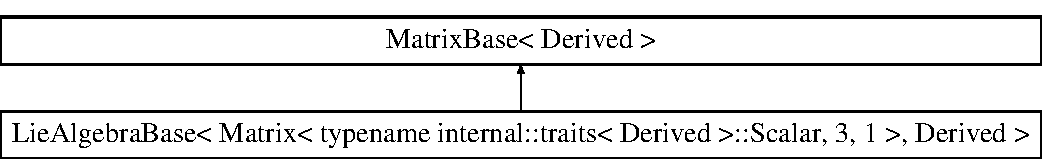
\includegraphics[height=2.000000cm]{class_lie_algebra_base_3_01_matrix_3_01typename_01internal_1_1traits_3_01_derived_01_4_1_1_scalabfa0bdce6d9781ee940346c3f6d91f4e}
\end{center}
\end{figure}
\subsection*{Public Types}
\begin{DoxyCompactItemize}
\item 
typedef Matrix$<$ Scalar, 3, 1 $>$ \hyperlink{class_lie_algebra_base_3_01_matrix_3_01typename_01internal_1_1traits_3_01_derived_01_4_1_1_scalabfa0bdce6d9781ee940346c3f6d91f4e_a2191d421225a2c966825db324301abba}{Base\+Type}
\item 
typedef internal\+::traits$<$ Derived $>$\+::\hyperlink{class_lie_algebra_base_3_01_matrix_3_01typename_01internal_1_1traits_3_01_derived_01_4_1_1_scalabfa0bdce6d9781ee940346c3f6d91f4e_a36f132794b928bcf1f707bf88d392288}{Coefficients} \hyperlink{class_lie_algebra_base_3_01_matrix_3_01typename_01internal_1_1traits_3_01_derived_01_4_1_1_scalabfa0bdce6d9781ee940346c3f6d91f4e_a36f132794b928bcf1f707bf88d392288}{Coefficients}
\item 
typedef \hyperlink{class_lie_algebra}{Lie\+Algebra}$<$ \hyperlink{class_lie_algebra_base_3_01_matrix_3_01typename_01internal_1_1traits_3_01_derived_01_4_1_1_scalabfa0bdce6d9781ee940346c3f6d91f4e_a2191d421225a2c966825db324301abba}{Base\+Type} $>$ \hyperlink{class_lie_algebra_base_3_01_matrix_3_01typename_01internal_1_1traits_3_01_derived_01_4_1_1_scalabfa0bdce6d9781ee940346c3f6d91f4e_a94a8de5117cf8e3142a6ceab24c1f5c2}{Plain\+Object}
\item 
typedef \hyperlink{class_lie_algebra_dual}{Lie\+Algebra\+Dual}$<$ \hyperlink{class_lie_algebra_base_3_01_matrix_3_01typename_01internal_1_1traits_3_01_derived_01_4_1_1_scalabfa0bdce6d9781ee940346c3f6d91f4e_a2191d421225a2c966825db324301abba}{Base\+Type} $>$ \hyperlink{class_lie_algebra_base_3_01_matrix_3_01typename_01internal_1_1traits_3_01_derived_01_4_1_1_scalabfa0bdce6d9781ee940346c3f6d91f4e_abe2ee13078cb63c23731c4b3af7b02cd}{Algebra\+Dual}
\item 
typedef internal\+::traits$<$ Derived $>$\+::\hyperlink{class_lie_algebra_base_3_01_matrix_3_01typename_01internal_1_1traits_3_01_derived_01_4_1_1_scalabfa0bdce6d9781ee940346c3f6d91f4e_ac400b52908b18fbf91ce3f942c2841e9}{Group} \hyperlink{class_lie_algebra_base_3_01_matrix_3_01typename_01internal_1_1traits_3_01_derived_01_4_1_1_scalabfa0bdce6d9781ee940346c3f6d91f4e_ac400b52908b18fbf91ce3f942c2841e9}{Group}
\item 
typedef Matrix$<$ Scalar, 3, 3 $>$ \hyperlink{class_lie_algebra_base_3_01_matrix_3_01typename_01internal_1_1traits_3_01_derived_01_4_1_1_scalabfa0bdce6d9781ee940346c3f6d91f4e_a76b0bda7b6a5390a434df96474c582db}{Matrix3}
\end{DoxyCompactItemize}
\subsection*{Public Member Functions}
\begin{DoxyCompactItemize}
\item 
E\+I\+G\+E\+N\+\_\+\+S\+T\+R\+O\+N\+G\+\_\+\+I\+N\+L\+I\+NE \hyperlink{class_lie_algebra_base}{Lie\+Algebra\+Base} \& \hyperlink{class_lie_algebra_base_3_01_matrix_3_01typename_01internal_1_1traits_3_01_derived_01_4_1_1_scalabfa0bdce6d9781ee940346c3f6d91f4e_aa1e456962c1fc5198a19c438f6dfca4a}{operator=} (const \hyperlink{class_lie_algebra_base}{Lie\+Algebra\+Base} \&other)
\item 
{\footnotesize template$<$class Other\+Derived $>$ }\\E\+I\+G\+E\+N\+\_\+\+S\+T\+R\+O\+N\+G\+\_\+\+I\+N\+L\+I\+NE Derived \& \hyperlink{class_lie_algebra_base_3_01_matrix_3_01typename_01internal_1_1traits_3_01_derived_01_4_1_1_scalabfa0bdce6d9781ee940346c3f6d91f4e_a04876d813c2cd5c25150f4028ba048ca}{operator=} (const \hyperlink{class_lie_algebra_base}{Lie\+Algebra\+Base}$<$ \hyperlink{class_lie_algebra_base_3_01_matrix_3_01typename_01internal_1_1traits_3_01_derived_01_4_1_1_scalabfa0bdce6d9781ee940346c3f6d91f4e_a2191d421225a2c966825db324301abba}{Base\+Type}, Other\+Derived $>$ \&other)
\item 
{\footnotesize template$<$class Other\+Derived $>$ }\\E\+I\+G\+E\+N\+\_\+\+S\+T\+R\+O\+N\+G\+\_\+\+I\+N\+L\+I\+NE Derived \& \hyperlink{class_lie_algebra_base_3_01_matrix_3_01typename_01internal_1_1traits_3_01_derived_01_4_1_1_scalabfa0bdce6d9781ee940346c3f6d91f4e_a91c3f4ab0fef7eddac375d0909f47bf2}{operator=} (const Matrix\+Base$<$ Other\+Derived $>$ \&other)
\item 
{\footnotesize template$<$class Other\+Derived $>$ }\\\hyperlink{class_lie_algebra_base_3_01_matrix_3_01typename_01internal_1_1traits_3_01_derived_01_4_1_1_scalabfa0bdce6d9781ee940346c3f6d91f4e_a94a8de5117cf8e3142a6ceab24c1f5c2}{Plain\+Object} \hyperlink{class_lie_algebra_base_3_01_matrix_3_01typename_01internal_1_1traits_3_01_derived_01_4_1_1_scalabfa0bdce6d9781ee940346c3f6d91f4e_afa135aa64acf6e927c6104b1fa8ce4bf}{bracket} (const \hyperlink{class_lie_algebra_base}{Lie\+Algebra\+Base}$<$ \hyperlink{class_lie_algebra_base_3_01_matrix_3_01typename_01internal_1_1traits_3_01_derived_01_4_1_1_scalabfa0bdce6d9781ee940346c3f6d91f4e_a2191d421225a2c966825db324301abba}{Base\+Type}, Other\+Derived $>$ \&a) const
\item 
\hyperlink{class_lie_algebra_base_3_01_matrix_3_01typename_01internal_1_1traits_3_01_derived_01_4_1_1_scalabfa0bdce6d9781ee940346c3f6d91f4e_ac400b52908b18fbf91ce3f942c2841e9}{Group} \hyperlink{class_lie_algebra_base_3_01_matrix_3_01typename_01internal_1_1traits_3_01_derived_01_4_1_1_scalabfa0bdce6d9781ee940346c3f6d91f4e_ae6f9ae43344c5314bb25ffd8d9df3b6b}{exp} (Scalar precision=1.e-\/5) const
\item 
Matrix$<$ Scalar, 3, 3 $>$ \hyperlink{class_lie_algebra_base_3_01_matrix_3_01typename_01internal_1_1traits_3_01_derived_01_4_1_1_scalabfa0bdce6d9781ee940346c3f6d91f4e_a8b415ebfce966f09b845e7094bc4779b}{dexp} (Scalar precision=1.e-\/6, Scalar precision2=1.e-\/2) const
\item 
{\footnotesize template$<$class Other\+Derived $>$ }\\Matrix$<$ Scalar, 3, 3 $>$ \hyperlink{class_lie_algebra_base_3_01_matrix_3_01typename_01internal_1_1traits_3_01_derived_01_4_1_1_scalabfa0bdce6d9781ee940346c3f6d91f4e_a9fb9f5bfa1694d5f7a68ee8ff6be1ed3}{d2exp} (const Matrix\+Base$<$ Other\+Derived $>$ \&v, Scalar precision=1.e-\/6, Scalar precision2=1.e-\/2) const
\item 
\hyperlink{class_lie_algebra_base_3_01_matrix_3_01typename_01internal_1_1traits_3_01_derived_01_4_1_1_scalabfa0bdce6d9781ee940346c3f6d91f4e_a36f132794b928bcf1f707bf88d392288}{Coefficients} \& \hyperlink{class_lie_algebra_base_3_01_matrix_3_01typename_01internal_1_1traits_3_01_derived_01_4_1_1_scalabfa0bdce6d9781ee940346c3f6d91f4e_a087b980c393345af2614f8a7ee5fb45f}{get} ()
\item 
const \hyperlink{class_lie_algebra_base_3_01_matrix_3_01typename_01internal_1_1traits_3_01_derived_01_4_1_1_scalabfa0bdce6d9781ee940346c3f6d91f4e_a36f132794b928bcf1f707bf88d392288}{Coefficients} \& \hyperlink{class_lie_algebra_base_3_01_matrix_3_01typename_01internal_1_1traits_3_01_derived_01_4_1_1_scalabfa0bdce6d9781ee940346c3f6d91f4e_aaf1d1fb3045b05a1a3ab60dbaeaf8a6b}{get} () const
\item 
{\footnotesize template$<$class Other\+Derived $>$ }\\Derived \& \hyperlink{class_lie_algebra_base_3_01_matrix_3_01typename_01internal_1_1traits_3_01_derived_01_4_1_1_scalabfa0bdce6d9781ee940346c3f6d91f4e_a71ba9feff1ba5b3337ad41a9537846f4}{operator=} (const \hyperlink{class_lie_algebra_base}{Lie\+Algebra\+Base}$<$ \hyperlink{class_lie_algebra_base_3_01_matrix_3_01typename_01internal_1_1traits_3_01_derived_01_4_1_1_scalabfa0bdce6d9781ee940346c3f6d91f4e_a2191d421225a2c966825db324301abba}{Base\+Type}, Other\+Derived $>$ \&other)
\item 
{\footnotesize template$<$class Other\+Derived $>$ }\\\hyperlink{class_lie_algebra_base}{Lie\+Algebra\+Base}$<$ Matrix$<$ typename internal\+::traits$<$ Derived $>$\+::Scalar, 3, 1 $>$, Derived $>$\+::\hyperlink{class_lie_algebra_base_3_01_matrix_3_01typename_01internal_1_1traits_3_01_derived_01_4_1_1_scalabfa0bdce6d9781ee940346c3f6d91f4e_a76b0bda7b6a5390a434df96474c582db}{Matrix3} \hyperlink{class_lie_algebra_base_3_01_matrix_3_01typename_01internal_1_1traits_3_01_derived_01_4_1_1_scalabfa0bdce6d9781ee940346c3f6d91f4e_a8fec2455fc2fca1f7d4683b1f78d67ec}{d2exp} (const Matrix\+Base$<$ Other\+Derived $>$ \&vec, Scalar precision, Scalar precision2) const
\end{DoxyCompactItemize}
\subsection*{Protected Types}
\begin{DoxyCompactItemize}
\item 
typedef Matrix\+Base$<$ Derived $>$ \hyperlink{class_lie_algebra_base_3_01_matrix_3_01typename_01internal_1_1traits_3_01_derived_01_4_1_1_scalabfa0bdce6d9781ee940346c3f6d91f4e_a732476e0ccd5638bf791f9f7a4c59f26}{Base}
\end{DoxyCompactItemize}


\subsection{Detailed Description}
\subsubsection*{template$<$class Derived$>$\newline
class Lie\+Algebra\+Base$<$ Matrix$<$ typename internal\+::traits$<$ Derived $>$\+::\+Scalar, 3, 1 $>$, Derived $>$}

Base class for the Lie Algebra so(3). 


\begin{DoxyTemplParams}{Template Parameters}
{\em Derived} & the derived class holding the coefficients which are of type Array$<$\+Scalar, 3, 1$>$ or Map$<$Array$<$\+Scalar, 3, 1$>$ $>$\\
\hline
\end{DoxyTemplParams}
This class actually implements methods form \hyperlink{class_lie_algebra_base}{Lie\+Algebra\+Base} for so(3)

Since a Lie Algebra is a vector Space (check if it\textquotesingle{}s true in the general case) it\textquotesingle{}s inherited from Matrix\+Base 

Definition at line 60 of file Lie\+Algebra\+\_\+so3.\+h.



\subsection{Member Typedef Documentation}
\hypertarget{class_lie_algebra_base_3_01_matrix_3_01typename_01internal_1_1traits_3_01_derived_01_4_1_1_scalabfa0bdce6d9781ee940346c3f6d91f4e_abe2ee13078cb63c23731c4b3af7b02cd}{}\label{class_lie_algebra_base_3_01_matrix_3_01typename_01internal_1_1traits_3_01_derived_01_4_1_1_scalabfa0bdce6d9781ee940346c3f6d91f4e_abe2ee13078cb63c23731c4b3af7b02cd} 
\index{Lie\+Algebra\+Base$<$ Matrix$<$ typename internal\+::traits$<$ Derived $>$\+::\+Scalar, 3, 1 $>$, Derived $>$@{Lie\+Algebra\+Base$<$ Matrix$<$ typename internal\+::traits$<$ Derived $>$\+::\+Scalar, 3, 1 $>$, Derived $>$}!Algebra\+Dual@{Algebra\+Dual}}
\index{Algebra\+Dual@{Algebra\+Dual}!Lie\+Algebra\+Base$<$ Matrix$<$ typename internal\+::traits$<$ Derived $>$\+::\+Scalar, 3, 1 $>$, Derived $>$@{Lie\+Algebra\+Base$<$ Matrix$<$ typename internal\+::traits$<$ Derived $>$\+::\+Scalar, 3, 1 $>$, Derived $>$}}
\subsubsection{\texorpdfstring{Algebra\+Dual}{AlgebraDual}}
{\footnotesize\ttfamily template$<$class Derived $>$ \\
typedef \hyperlink{class_lie_algebra_dual}{Lie\+Algebra\+Dual}$<$\hyperlink{class_lie_algebra_base_3_01_matrix_3_01typename_01internal_1_1traits_3_01_derived_01_4_1_1_scalabfa0bdce6d9781ee940346c3f6d91f4e_a2191d421225a2c966825db324301abba}{Base\+Type}$>$ \hyperlink{class_lie_algebra_base}{Lie\+Algebra\+Base}$<$ Matrix$<$ typename internal\+::traits$<$ Derived $>$\+::Scalar, 3, 1 $>$, Derived $>$\+::\hyperlink{class_lie_algebra_base_3_01_matrix_3_01typename_01internal_1_1traits_3_01_derived_01_4_1_1_scalabfa0bdce6d9781ee940346c3f6d91f4e_abe2ee13078cb63c23731c4b3af7b02cd}{Algebra\+Dual}}

The type of the dual Algebra 

Definition at line 81 of file Lie\+Algebra\+\_\+so3.\+h.

\hypertarget{class_lie_algebra_base_3_01_matrix_3_01typename_01internal_1_1traits_3_01_derived_01_4_1_1_scalabfa0bdce6d9781ee940346c3f6d91f4e_a732476e0ccd5638bf791f9f7a4c59f26}{}\label{class_lie_algebra_base_3_01_matrix_3_01typename_01internal_1_1traits_3_01_derived_01_4_1_1_scalabfa0bdce6d9781ee940346c3f6d91f4e_a732476e0ccd5638bf791f9f7a4c59f26} 
\index{Lie\+Algebra\+Base$<$ Matrix$<$ typename internal\+::traits$<$ Derived $>$\+::\+Scalar, 3, 1 $>$, Derived $>$@{Lie\+Algebra\+Base$<$ Matrix$<$ typename internal\+::traits$<$ Derived $>$\+::\+Scalar, 3, 1 $>$, Derived $>$}!Base@{Base}}
\index{Base@{Base}!Lie\+Algebra\+Base$<$ Matrix$<$ typename internal\+::traits$<$ Derived $>$\+::\+Scalar, 3, 1 $>$, Derived $>$@{Lie\+Algebra\+Base$<$ Matrix$<$ typename internal\+::traits$<$ Derived $>$\+::\+Scalar, 3, 1 $>$, Derived $>$}}
\subsubsection{\texorpdfstring{Base}{Base}}
{\footnotesize\ttfamily template$<$class Derived $>$ \\
typedef Matrix\+Base$<$Derived$>$ \hyperlink{class_lie_algebra_base}{Lie\+Algebra\+Base}$<$ Matrix$<$ typename internal\+::traits$<$ Derived $>$\+::Scalar, 3, 1 $>$, Derived $>$\+::\hyperlink{class_lie_algebra_base_3_01_matrix_3_01typename_01internal_1_1traits_3_01_derived_01_4_1_1_scalabfa0bdce6d9781ee940346c3f6d91f4e_a732476e0ccd5638bf791f9f7a4c59f26}{Base}\hspace{0.3cm}{\ttfamily [protected]}}

The inherited class 

Definition at line 65 of file Lie\+Algebra\+\_\+so3.\+h.

\hypertarget{class_lie_algebra_base_3_01_matrix_3_01typename_01internal_1_1traits_3_01_derived_01_4_1_1_scalabfa0bdce6d9781ee940346c3f6d91f4e_a2191d421225a2c966825db324301abba}{}\label{class_lie_algebra_base_3_01_matrix_3_01typename_01internal_1_1traits_3_01_derived_01_4_1_1_scalabfa0bdce6d9781ee940346c3f6d91f4e_a2191d421225a2c966825db324301abba} 
\index{Lie\+Algebra\+Base$<$ Matrix$<$ typename internal\+::traits$<$ Derived $>$\+::\+Scalar, 3, 1 $>$, Derived $>$@{Lie\+Algebra\+Base$<$ Matrix$<$ typename internal\+::traits$<$ Derived $>$\+::\+Scalar, 3, 1 $>$, Derived $>$}!Base\+Type@{Base\+Type}}
\index{Base\+Type@{Base\+Type}!Lie\+Algebra\+Base$<$ Matrix$<$ typename internal\+::traits$<$ Derived $>$\+::\+Scalar, 3, 1 $>$, Derived $>$@{Lie\+Algebra\+Base$<$ Matrix$<$ typename internal\+::traits$<$ Derived $>$\+::\+Scalar, 3, 1 $>$, Derived $>$}}
\subsubsection{\texorpdfstring{Base\+Type}{BaseType}}
{\footnotesize\ttfamily template$<$class Derived $>$ \\
typedef Matrix$<$Scalar, 3, 1$>$ \hyperlink{class_lie_algebra_base}{Lie\+Algebra\+Base}$<$ Matrix$<$ typename internal\+::traits$<$ Derived $>$\+::Scalar, 3, 1 $>$, Derived $>$\+::\hyperlink{class_lie_algebra_base_3_01_matrix_3_01typename_01internal_1_1traits_3_01_derived_01_4_1_1_scalabfa0bdce6d9781ee940346c3f6d91f4e_a2191d421225a2c966825db324301abba}{Base\+Type}}

The wrapped class 

Definition at line 75 of file Lie\+Algebra\+\_\+so3.\+h.

\hypertarget{class_lie_algebra_base_3_01_matrix_3_01typename_01internal_1_1traits_3_01_derived_01_4_1_1_scalabfa0bdce6d9781ee940346c3f6d91f4e_a36f132794b928bcf1f707bf88d392288}{}\label{class_lie_algebra_base_3_01_matrix_3_01typename_01internal_1_1traits_3_01_derived_01_4_1_1_scalabfa0bdce6d9781ee940346c3f6d91f4e_a36f132794b928bcf1f707bf88d392288} 
\index{Lie\+Algebra\+Base$<$ Matrix$<$ typename internal\+::traits$<$ Derived $>$\+::\+Scalar, 3, 1 $>$, Derived $>$@{Lie\+Algebra\+Base$<$ Matrix$<$ typename internal\+::traits$<$ Derived $>$\+::\+Scalar, 3, 1 $>$, Derived $>$}!Coefficients@{Coefficients}}
\index{Coefficients@{Coefficients}!Lie\+Algebra\+Base$<$ Matrix$<$ typename internal\+::traits$<$ Derived $>$\+::\+Scalar, 3, 1 $>$, Derived $>$@{Lie\+Algebra\+Base$<$ Matrix$<$ typename internal\+::traits$<$ Derived $>$\+::\+Scalar, 3, 1 $>$, Derived $>$}}
\subsubsection{\texorpdfstring{Coefficients}{Coefficients}}
{\footnotesize\ttfamily template$<$class Derived $>$ \\
typedef internal\+::traits$<$Derived$>$\+::\hyperlink{class_lie_algebra_base_3_01_matrix_3_01typename_01internal_1_1traits_3_01_derived_01_4_1_1_scalabfa0bdce6d9781ee940346c3f6d91f4e_a36f132794b928bcf1f707bf88d392288}{Coefficients} \hyperlink{class_lie_algebra_base}{Lie\+Algebra\+Base}$<$ Matrix$<$ typename internal\+::traits$<$ Derived $>$\+::Scalar, 3, 1 $>$, Derived $>$\+::\hyperlink{class_lie_algebra_base_3_01_matrix_3_01typename_01internal_1_1traits_3_01_derived_01_4_1_1_scalabfa0bdce6d9781ee940346c3f6d91f4e_a36f132794b928bcf1f707bf88d392288}{Coefficients}}

The kind of stored coefficients 

Definition at line 77 of file Lie\+Algebra\+\_\+so3.\+h.

\hypertarget{class_lie_algebra_base_3_01_matrix_3_01typename_01internal_1_1traits_3_01_derived_01_4_1_1_scalabfa0bdce6d9781ee940346c3f6d91f4e_ac400b52908b18fbf91ce3f942c2841e9}{}\label{class_lie_algebra_base_3_01_matrix_3_01typename_01internal_1_1traits_3_01_derived_01_4_1_1_scalabfa0bdce6d9781ee940346c3f6d91f4e_ac400b52908b18fbf91ce3f942c2841e9} 
\index{Lie\+Algebra\+Base$<$ Matrix$<$ typename internal\+::traits$<$ Derived $>$\+::\+Scalar, 3, 1 $>$, Derived $>$@{Lie\+Algebra\+Base$<$ Matrix$<$ typename internal\+::traits$<$ Derived $>$\+::\+Scalar, 3, 1 $>$, Derived $>$}!Group@{Group}}
\index{Group@{Group}!Lie\+Algebra\+Base$<$ Matrix$<$ typename internal\+::traits$<$ Derived $>$\+::\+Scalar, 3, 1 $>$, Derived $>$@{Lie\+Algebra\+Base$<$ Matrix$<$ typename internal\+::traits$<$ Derived $>$\+::\+Scalar, 3, 1 $>$, Derived $>$}}
\subsubsection{\texorpdfstring{Group}{Group}}
{\footnotesize\ttfamily template$<$class Derived $>$ \\
typedef internal\+::traits$<$Derived$>$\+::\hyperlink{class_lie_algebra_base_3_01_matrix_3_01typename_01internal_1_1traits_3_01_derived_01_4_1_1_scalabfa0bdce6d9781ee940346c3f6d91f4e_ac400b52908b18fbf91ce3f942c2841e9}{Group} \hyperlink{class_lie_algebra_base}{Lie\+Algebra\+Base}$<$ Matrix$<$ typename internal\+::traits$<$ Derived $>$\+::Scalar, 3, 1 $>$, Derived $>$\+::\hyperlink{class_lie_algebra_base_3_01_matrix_3_01typename_01internal_1_1traits_3_01_derived_01_4_1_1_scalabfa0bdce6d9781ee940346c3f6d91f4e_ac400b52908b18fbf91ce3f942c2841e9}{Group}}

The type of the associated Lie Group 

Definition at line 83 of file Lie\+Algebra\+\_\+so3.\+h.

\hypertarget{class_lie_algebra_base_3_01_matrix_3_01typename_01internal_1_1traits_3_01_derived_01_4_1_1_scalabfa0bdce6d9781ee940346c3f6d91f4e_a76b0bda7b6a5390a434df96474c582db}{}\label{class_lie_algebra_base_3_01_matrix_3_01typename_01internal_1_1traits_3_01_derived_01_4_1_1_scalabfa0bdce6d9781ee940346c3f6d91f4e_a76b0bda7b6a5390a434df96474c582db} 
\index{Lie\+Algebra\+Base$<$ Matrix$<$ typename internal\+::traits$<$ Derived $>$\+::\+Scalar, 3, 1 $>$, Derived $>$@{Lie\+Algebra\+Base$<$ Matrix$<$ typename internal\+::traits$<$ Derived $>$\+::\+Scalar, 3, 1 $>$, Derived $>$}!Matrix3@{Matrix3}}
\index{Matrix3@{Matrix3}!Lie\+Algebra\+Base$<$ Matrix$<$ typename internal\+::traits$<$ Derived $>$\+::\+Scalar, 3, 1 $>$, Derived $>$@{Lie\+Algebra\+Base$<$ Matrix$<$ typename internal\+::traits$<$ Derived $>$\+::\+Scalar, 3, 1 $>$, Derived $>$}}
\subsubsection{\texorpdfstring{Matrix3}{Matrix3}}
{\footnotesize\ttfamily template$<$class Derived $>$ \\
typedef Matrix$<$Scalar, 3, 3$>$ \hyperlink{class_lie_algebra_base}{Lie\+Algebra\+Base}$<$ Matrix$<$ typename internal\+::traits$<$ Derived $>$\+::Scalar, 3, 1 $>$, Derived $>$\+::\hyperlink{class_lie_algebra_base_3_01_matrix_3_01typename_01internal_1_1traits_3_01_derived_01_4_1_1_scalabfa0bdce6d9781ee940346c3f6d91f4e_a76b0bda7b6a5390a434df96474c582db}{Matrix3}}

The type of the matrix return by derivatives of exp 

Definition at line 85 of file Lie\+Algebra\+\_\+so3.\+h.

\hypertarget{class_lie_algebra_base_3_01_matrix_3_01typename_01internal_1_1traits_3_01_derived_01_4_1_1_scalabfa0bdce6d9781ee940346c3f6d91f4e_a94a8de5117cf8e3142a6ceab24c1f5c2}{}\label{class_lie_algebra_base_3_01_matrix_3_01typename_01internal_1_1traits_3_01_derived_01_4_1_1_scalabfa0bdce6d9781ee940346c3f6d91f4e_a94a8de5117cf8e3142a6ceab24c1f5c2} 
\index{Lie\+Algebra\+Base$<$ Matrix$<$ typename internal\+::traits$<$ Derived $>$\+::\+Scalar, 3, 1 $>$, Derived $>$@{Lie\+Algebra\+Base$<$ Matrix$<$ typename internal\+::traits$<$ Derived $>$\+::\+Scalar, 3, 1 $>$, Derived $>$}!Plain\+Object@{Plain\+Object}}
\index{Plain\+Object@{Plain\+Object}!Lie\+Algebra\+Base$<$ Matrix$<$ typename internal\+::traits$<$ Derived $>$\+::\+Scalar, 3, 1 $>$, Derived $>$@{Lie\+Algebra\+Base$<$ Matrix$<$ typename internal\+::traits$<$ Derived $>$\+::\+Scalar, 3, 1 $>$, Derived $>$}}
\subsubsection{\texorpdfstring{Plain\+Object}{PlainObject}}
{\footnotesize\ttfamily template$<$class Derived $>$ \\
typedef \hyperlink{class_lie_algebra}{Lie\+Algebra}$<$\hyperlink{class_lie_algebra_base_3_01_matrix_3_01typename_01internal_1_1traits_3_01_derived_01_4_1_1_scalabfa0bdce6d9781ee940346c3f6d91f4e_a2191d421225a2c966825db324301abba}{Base\+Type}$>$ \hyperlink{class_lie_algebra_base}{Lie\+Algebra\+Base}$<$ Matrix$<$ typename internal\+::traits$<$ Derived $>$\+::Scalar, 3, 1 $>$, Derived $>$\+::\hyperlink{class_lie_algebra_base_3_01_matrix_3_01typename_01internal_1_1traits_3_01_derived_01_4_1_1_scalabfa0bdce6d9781ee940346c3f6d91f4e_a94a8de5117cf8e3142a6ceab24c1f5c2}{Plain\+Object}}

The plain object returned, while using Map$<$Lie\+Algebra$<$ $>$ $>$ 

Definition at line 79 of file Lie\+Algebra\+\_\+so3.\+h.



\subsection{Member Function Documentation}
\hypertarget{class_lie_algebra_base_3_01_matrix_3_01typename_01internal_1_1traits_3_01_derived_01_4_1_1_scalabfa0bdce6d9781ee940346c3f6d91f4e_afa135aa64acf6e927c6104b1fa8ce4bf}{}\label{class_lie_algebra_base_3_01_matrix_3_01typename_01internal_1_1traits_3_01_derived_01_4_1_1_scalabfa0bdce6d9781ee940346c3f6d91f4e_afa135aa64acf6e927c6104b1fa8ce4bf} 
\index{Lie\+Algebra\+Base$<$ Matrix$<$ typename internal\+::traits$<$ Derived $>$\+::\+Scalar, 3, 1 $>$, Derived $>$@{Lie\+Algebra\+Base$<$ Matrix$<$ typename internal\+::traits$<$ Derived $>$\+::\+Scalar, 3, 1 $>$, Derived $>$}!bracket@{bracket}}
\index{bracket@{bracket}!Lie\+Algebra\+Base$<$ Matrix$<$ typename internal\+::traits$<$ Derived $>$\+::\+Scalar, 3, 1 $>$, Derived $>$@{Lie\+Algebra\+Base$<$ Matrix$<$ typename internal\+::traits$<$ Derived $>$\+::\+Scalar, 3, 1 $>$, Derived $>$}}
\subsubsection{\texorpdfstring{bracket()}{bracket()}}
{\footnotesize\ttfamily template$<$class Derived $>$ \\
template$<$class Other\+Derived $>$ \\
\hyperlink{class_lie_algebra_base}{Lie\+Algebra\+Base}$<$ Matrix$<$ typename internal\+::traits$<$ Derived $>$\+::Scalar, 3, 1 $>$, Derived $>$\+::\hyperlink{class_lie_algebra_base_3_01_matrix_3_01typename_01internal_1_1traits_3_01_derived_01_4_1_1_scalabfa0bdce6d9781ee940346c3f6d91f4e_a94a8de5117cf8e3142a6ceab24c1f5c2}{Plain\+Object} \hyperlink{class_lie_algebra_base}{Lie\+Algebra\+Base}$<$ Matrix$<$ typename internal\+::traits$<$ Derived $>$\+::Scalar, 3, 1 $>$, Derived $>$\+::bracket (\begin{DoxyParamCaption}\item[{const \hyperlink{class_lie_algebra_base}{Lie\+Algebra\+Base}$<$ \hyperlink{class_lie_algebra_base_3_01_matrix_3_01typename_01internal_1_1traits_3_01_derived_01_4_1_1_scalabfa0bdce6d9781ee940346c3f6d91f4e_a2191d421225a2c966825db324301abba}{Base\+Type}, Other\+Derived $>$ \&}]{a }\end{DoxyParamCaption}) const\hspace{0.3cm}{\ttfamily [inline]}}

Lie Bracket 

Definition at line 147 of file Lie\+Algebra\+\_\+so3.\+h.

\hypertarget{class_lie_algebra_base_3_01_matrix_3_01typename_01internal_1_1traits_3_01_derived_01_4_1_1_scalabfa0bdce6d9781ee940346c3f6d91f4e_a9fb9f5bfa1694d5f7a68ee8ff6be1ed3}{}\label{class_lie_algebra_base_3_01_matrix_3_01typename_01internal_1_1traits_3_01_derived_01_4_1_1_scalabfa0bdce6d9781ee940346c3f6d91f4e_a9fb9f5bfa1694d5f7a68ee8ff6be1ed3} 
\index{Lie\+Algebra\+Base$<$ Matrix$<$ typename internal\+::traits$<$ Derived $>$\+::\+Scalar, 3, 1 $>$, Derived $>$@{Lie\+Algebra\+Base$<$ Matrix$<$ typename internal\+::traits$<$ Derived $>$\+::\+Scalar, 3, 1 $>$, Derived $>$}!d2exp@{d2exp}}
\index{d2exp@{d2exp}!Lie\+Algebra\+Base$<$ Matrix$<$ typename internal\+::traits$<$ Derived $>$\+::\+Scalar, 3, 1 $>$, Derived $>$@{Lie\+Algebra\+Base$<$ Matrix$<$ typename internal\+::traits$<$ Derived $>$\+::\+Scalar, 3, 1 $>$, Derived $>$}}
\subsubsection{\texorpdfstring{d2exp()}{d2exp()}\hspace{0.1cm}{\footnotesize\ttfamily [1/2]}}
{\footnotesize\ttfamily template$<$class Derived $>$ \\
template$<$class Other\+Derived $>$ \\
Matrix$<$Scalar, 3, 3$>$ \hyperlink{class_lie_algebra_base}{Lie\+Algebra\+Base}$<$ Matrix$<$ typename internal\+::traits$<$ Derived $>$\+::Scalar, 3, 1 $>$, Derived $>$\+::d2exp (\begin{DoxyParamCaption}\item[{const Matrix\+Base$<$ Other\+Derived $>$ \&}]{v,  }\item[{Scalar}]{precision = {\ttfamily 1.e-\/6},  }\item[{Scalar}]{precision2 = {\ttfamily 1.e-\/2} }\end{DoxyParamCaption}) const\hspace{0.3cm}{\ttfamily [inline]}}

\begin{DoxyReturn}{Returns}
second derivative of exp along vector {\ttfamily v} 
\end{DoxyReturn}
\begin{DoxySeeAlso}{See also}
\hyperlink{class_lie_algebra_base_aafe7d43a29d43aed54dd91b3a3a4c9f7}{Lie\+Algebra\+Base\+::exp} 
\end{DoxySeeAlso}
\hypertarget{class_lie_algebra_base_3_01_matrix_3_01typename_01internal_1_1traits_3_01_derived_01_4_1_1_scalabfa0bdce6d9781ee940346c3f6d91f4e_a8fec2455fc2fca1f7d4683b1f78d67ec}{}\label{class_lie_algebra_base_3_01_matrix_3_01typename_01internal_1_1traits_3_01_derived_01_4_1_1_scalabfa0bdce6d9781ee940346c3f6d91f4e_a8fec2455fc2fca1f7d4683b1f78d67ec} 
\index{Lie\+Algebra\+Base$<$ Matrix$<$ typename internal\+::traits$<$ Derived $>$\+::\+Scalar, 3, 1 $>$, Derived $>$@{Lie\+Algebra\+Base$<$ Matrix$<$ typename internal\+::traits$<$ Derived $>$\+::\+Scalar, 3, 1 $>$, Derived $>$}!d2exp@{d2exp}}
\index{d2exp@{d2exp}!Lie\+Algebra\+Base$<$ Matrix$<$ typename internal\+::traits$<$ Derived $>$\+::\+Scalar, 3, 1 $>$, Derived $>$@{Lie\+Algebra\+Base$<$ Matrix$<$ typename internal\+::traits$<$ Derived $>$\+::\+Scalar, 3, 1 $>$, Derived $>$}}
\subsubsection{\texorpdfstring{d2exp()}{d2exp()}\hspace{0.1cm}{\footnotesize\ttfamily [2/2]}}
{\footnotesize\ttfamily template$<$class Derived $>$ \\
template$<$class Other\+Derived $>$ \\
\hyperlink{class_lie_algebra_base}{Lie\+Algebra\+Base}$<$Matrix$<$typename internal\+::traits$<$Derived$>$\+::Scalar, 3, 1$>$, Derived $>$\+::\hyperlink{class_lie_algebra_base_3_01_matrix_3_01typename_01internal_1_1traits_3_01_derived_01_4_1_1_scalabfa0bdce6d9781ee940346c3f6d91f4e_a76b0bda7b6a5390a434df96474c582db}{Matrix3} \hyperlink{class_lie_algebra_base}{Lie\+Algebra\+Base}$<$ Matrix$<$ typename internal\+::traits$<$ Derived $>$\+::Scalar, 3, 1 $>$, Derived $>$\+::d2exp (\begin{DoxyParamCaption}\item[{const Matrix\+Base$<$ Other\+Derived $>$ \&}]{vec,  }\item[{Scalar}]{precision,  }\item[{Scalar}]{precision2 }\end{DoxyParamCaption}) const\hspace{0.3cm}{\ttfamily [inline]}}



Definition at line 215 of file Lie\+Algebra\+\_\+so3.\+h.

\hypertarget{class_lie_algebra_base_3_01_matrix_3_01typename_01internal_1_1traits_3_01_derived_01_4_1_1_scalabfa0bdce6d9781ee940346c3f6d91f4e_a8b415ebfce966f09b845e7094bc4779b}{}\label{class_lie_algebra_base_3_01_matrix_3_01typename_01internal_1_1traits_3_01_derived_01_4_1_1_scalabfa0bdce6d9781ee940346c3f6d91f4e_a8b415ebfce966f09b845e7094bc4779b} 
\index{Lie\+Algebra\+Base$<$ Matrix$<$ typename internal\+::traits$<$ Derived $>$\+::\+Scalar, 3, 1 $>$, Derived $>$@{Lie\+Algebra\+Base$<$ Matrix$<$ typename internal\+::traits$<$ Derived $>$\+::\+Scalar, 3, 1 $>$, Derived $>$}!dexp@{dexp}}
\index{dexp@{dexp}!Lie\+Algebra\+Base$<$ Matrix$<$ typename internal\+::traits$<$ Derived $>$\+::\+Scalar, 3, 1 $>$, Derived $>$@{Lie\+Algebra\+Base$<$ Matrix$<$ typename internal\+::traits$<$ Derived $>$\+::\+Scalar, 3, 1 $>$, Derived $>$}}
\subsubsection{\texorpdfstring{dexp()}{dexp()}}
{\footnotesize\ttfamily template$<$class Derived $>$ \\
\hyperlink{class_lie_algebra_base}{Lie\+Algebra\+Base}$<$ Matrix$<$ typename internal\+::traits$<$ Derived $>$\+::Scalar, 3, 1 $>$, Derived $>$\+::\hyperlink{class_lie_algebra_base_3_01_matrix_3_01typename_01internal_1_1traits_3_01_derived_01_4_1_1_scalabfa0bdce6d9781ee940346c3f6d91f4e_a76b0bda7b6a5390a434df96474c582db}{Matrix3} \hyperlink{class_lie_algebra_base}{Lie\+Algebra\+Base}$<$ Matrix$<$ typename internal\+::traits$<$ Derived $>$\+::Scalar, 3, 1 $>$, Derived $>$\+::dexp (\begin{DoxyParamCaption}\item[{Scalar}]{precision = {\ttfamily 1.e-\/6},  }\item[{Scalar}]{precision2 = {\ttfamily 1.e-\/2} }\end{DoxyParamCaption}) const\hspace{0.3cm}{\ttfamily [inline]}}

\begin{DoxyReturn}{Returns}
the first derivative of exp 
\end{DoxyReturn}
\begin{DoxySeeAlso}{See also}
\hyperlink{class_lie_algebra_base_aafe7d43a29d43aed54dd91b3a3a4c9f7}{Lie\+Algebra\+Base\+::exp} 
\end{DoxySeeAlso}


Definition at line 182 of file Lie\+Algebra\+\_\+so3.\+h.

\hypertarget{class_lie_algebra_base_3_01_matrix_3_01typename_01internal_1_1traits_3_01_derived_01_4_1_1_scalabfa0bdce6d9781ee940346c3f6d91f4e_ae6f9ae43344c5314bb25ffd8d9df3b6b}{}\label{class_lie_algebra_base_3_01_matrix_3_01typename_01internal_1_1traits_3_01_derived_01_4_1_1_scalabfa0bdce6d9781ee940346c3f6d91f4e_ae6f9ae43344c5314bb25ffd8d9df3b6b} 
\index{Lie\+Algebra\+Base$<$ Matrix$<$ typename internal\+::traits$<$ Derived $>$\+::\+Scalar, 3, 1 $>$, Derived $>$@{Lie\+Algebra\+Base$<$ Matrix$<$ typename internal\+::traits$<$ Derived $>$\+::\+Scalar, 3, 1 $>$, Derived $>$}!exp@{exp}}
\index{exp@{exp}!Lie\+Algebra\+Base$<$ Matrix$<$ typename internal\+::traits$<$ Derived $>$\+::\+Scalar, 3, 1 $>$, Derived $>$@{Lie\+Algebra\+Base$<$ Matrix$<$ typename internal\+::traits$<$ Derived $>$\+::\+Scalar, 3, 1 $>$, Derived $>$}}
\subsubsection{\texorpdfstring{exp()}{exp()}}
{\footnotesize\ttfamily template$<$class Derived $>$ \\
\hyperlink{class_lie_algebra_base}{Lie\+Algebra\+Base}$<$ Matrix$<$ typename internal\+::traits$<$ Derived $>$\+::Scalar, 3, 1 $>$, Derived $>$\+::\hyperlink{class_lie_algebra_base_3_01_matrix_3_01typename_01internal_1_1traits_3_01_derived_01_4_1_1_scalabfa0bdce6d9781ee940346c3f6d91f4e_ac400b52908b18fbf91ce3f942c2841e9}{Group} \hyperlink{class_lie_algebra_base}{Lie\+Algebra\+Base}$<$ Matrix$<$ typename internal\+::traits$<$ Derived $>$\+::Scalar, 3, 1 $>$, Derived $>$\+::exp (\begin{DoxyParamCaption}\item[{Scalar}]{precision = {\ttfamily 1.e-\/5} }\end{DoxyParamCaption}) const\hspace{0.3cm}{\ttfamily [inline]}}

\begin{DoxyReturn}{Returns}
The element of the associated Lie Group through the exponential map 
\end{DoxyReturn}


Definition at line 162 of file Lie\+Algebra\+\_\+so3.\+h.

\hypertarget{class_lie_algebra_base_3_01_matrix_3_01typename_01internal_1_1traits_3_01_derived_01_4_1_1_scalabfa0bdce6d9781ee940346c3f6d91f4e_a087b980c393345af2614f8a7ee5fb45f}{}\label{class_lie_algebra_base_3_01_matrix_3_01typename_01internal_1_1traits_3_01_derived_01_4_1_1_scalabfa0bdce6d9781ee940346c3f6d91f4e_a087b980c393345af2614f8a7ee5fb45f} 
\index{Lie\+Algebra\+Base$<$ Matrix$<$ typename internal\+::traits$<$ Derived $>$\+::\+Scalar, 3, 1 $>$, Derived $>$@{Lie\+Algebra\+Base$<$ Matrix$<$ typename internal\+::traits$<$ Derived $>$\+::\+Scalar, 3, 1 $>$, Derived $>$}!get@{get}}
\index{get@{get}!Lie\+Algebra\+Base$<$ Matrix$<$ typename internal\+::traits$<$ Derived $>$\+::\+Scalar, 3, 1 $>$, Derived $>$@{Lie\+Algebra\+Base$<$ Matrix$<$ typename internal\+::traits$<$ Derived $>$\+::\+Scalar, 3, 1 $>$, Derived $>$}}
\subsubsection{\texorpdfstring{get()}{get()}\hspace{0.1cm}{\footnotesize\ttfamily [1/2]}}
{\footnotesize\ttfamily template$<$class Derived $>$ \\
\hyperlink{class_lie_algebra_base_3_01_matrix_3_01typename_01internal_1_1traits_3_01_derived_01_4_1_1_scalabfa0bdce6d9781ee940346c3f6d91f4e_a36f132794b928bcf1f707bf88d392288}{Coefficients}\& \hyperlink{class_lie_algebra_base}{Lie\+Algebra\+Base}$<$ Matrix$<$ typename internal\+::traits$<$ Derived $>$\+::Scalar, 3, 1 $>$, Derived $>$\+::get (\begin{DoxyParamCaption}{ }\end{DoxyParamCaption})\hspace{0.3cm}{\ttfamily [inline]}}

\begin{DoxyReturn}{Returns}
The stored coefficients 
\end{DoxyReturn}


Definition at line 115 of file Lie\+Algebra\+\_\+so3.\+h.

\hypertarget{class_lie_algebra_base_3_01_matrix_3_01typename_01internal_1_1traits_3_01_derived_01_4_1_1_scalabfa0bdce6d9781ee940346c3f6d91f4e_aaf1d1fb3045b05a1a3ab60dbaeaf8a6b}{}\label{class_lie_algebra_base_3_01_matrix_3_01typename_01internal_1_1traits_3_01_derived_01_4_1_1_scalabfa0bdce6d9781ee940346c3f6d91f4e_aaf1d1fb3045b05a1a3ab60dbaeaf8a6b} 
\index{Lie\+Algebra\+Base$<$ Matrix$<$ typename internal\+::traits$<$ Derived $>$\+::\+Scalar, 3, 1 $>$, Derived $>$@{Lie\+Algebra\+Base$<$ Matrix$<$ typename internal\+::traits$<$ Derived $>$\+::\+Scalar, 3, 1 $>$, Derived $>$}!get@{get}}
\index{get@{get}!Lie\+Algebra\+Base$<$ Matrix$<$ typename internal\+::traits$<$ Derived $>$\+::\+Scalar, 3, 1 $>$, Derived $>$@{Lie\+Algebra\+Base$<$ Matrix$<$ typename internal\+::traits$<$ Derived $>$\+::\+Scalar, 3, 1 $>$, Derived $>$}}
\subsubsection{\texorpdfstring{get()}{get()}\hspace{0.1cm}{\footnotesize\ttfamily [2/2]}}
{\footnotesize\ttfamily template$<$class Derived $>$ \\
const \hyperlink{class_lie_algebra_base_3_01_matrix_3_01typename_01internal_1_1traits_3_01_derived_01_4_1_1_scalabfa0bdce6d9781ee940346c3f6d91f4e_a36f132794b928bcf1f707bf88d392288}{Coefficients}\& \hyperlink{class_lie_algebra_base}{Lie\+Algebra\+Base}$<$ Matrix$<$ typename internal\+::traits$<$ Derived $>$\+::Scalar, 3, 1 $>$, Derived $>$\+::get (\begin{DoxyParamCaption}{ }\end{DoxyParamCaption}) const\hspace{0.3cm}{\ttfamily [inline]}}

\begin{DoxyReturn}{Returns}
The read-\/only access to the stored coefficients 
\end{DoxyReturn}


Definition at line 117 of file Lie\+Algebra\+\_\+so3.\+h.

\hypertarget{class_lie_algebra_base_3_01_matrix_3_01typename_01internal_1_1traits_3_01_derived_01_4_1_1_scalabfa0bdce6d9781ee940346c3f6d91f4e_aa1e456962c1fc5198a19c438f6dfca4a}{}\label{class_lie_algebra_base_3_01_matrix_3_01typename_01internal_1_1traits_3_01_derived_01_4_1_1_scalabfa0bdce6d9781ee940346c3f6d91f4e_aa1e456962c1fc5198a19c438f6dfca4a} 
\index{Lie\+Algebra\+Base$<$ Matrix$<$ typename internal\+::traits$<$ Derived $>$\+::\+Scalar, 3, 1 $>$, Derived $>$@{Lie\+Algebra\+Base$<$ Matrix$<$ typename internal\+::traits$<$ Derived $>$\+::\+Scalar, 3, 1 $>$, Derived $>$}!operator=@{operator=}}
\index{operator=@{operator=}!Lie\+Algebra\+Base$<$ Matrix$<$ typename internal\+::traits$<$ Derived $>$\+::\+Scalar, 3, 1 $>$, Derived $>$@{Lie\+Algebra\+Base$<$ Matrix$<$ typename internal\+::traits$<$ Derived $>$\+::\+Scalar, 3, 1 $>$, Derived $>$}}
\subsubsection{\texorpdfstring{operator=()}{operator=()}\hspace{0.1cm}{\footnotesize\ttfamily [1/4]}}
{\footnotesize\ttfamily template$<$class Derived $>$ \\
\hyperlink{class_lie_algebra_base}{Lie\+Algebra\+Base}$<$ Matrix$<$ typename internal\+::traits$<$ Derived $>$\+::Scalar, 3, 1 $>$, Derived $>$ \& \hyperlink{class_lie_algebra_base}{Lie\+Algebra\+Base}$<$ Matrix$<$ typename internal\+::traits$<$ Derived $>$\+::Scalar, 3, 1 $>$, Derived $>$\+::operator= (\begin{DoxyParamCaption}\item[{const \hyperlink{class_lie_algebra_base}{Lie\+Algebra\+Base}$<$ Matrix$<$ typename internal\+::traits$<$ Derived $>$\+::Scalar, 3, 1 $>$, Derived $>$ \&}]{other }\end{DoxyParamCaption})\hspace{0.3cm}{\ttfamily [inline]}}

Default assignement operator 

Definition at line 128 of file Lie\+Algebra\+\_\+so3.\+h.

\hypertarget{class_lie_algebra_base_3_01_matrix_3_01typename_01internal_1_1traits_3_01_derived_01_4_1_1_scalabfa0bdce6d9781ee940346c3f6d91f4e_a04876d813c2cd5c25150f4028ba048ca}{}\label{class_lie_algebra_base_3_01_matrix_3_01typename_01internal_1_1traits_3_01_derived_01_4_1_1_scalabfa0bdce6d9781ee940346c3f6d91f4e_a04876d813c2cd5c25150f4028ba048ca} 
\index{Lie\+Algebra\+Base$<$ Matrix$<$ typename internal\+::traits$<$ Derived $>$\+::\+Scalar, 3, 1 $>$, Derived $>$@{Lie\+Algebra\+Base$<$ Matrix$<$ typename internal\+::traits$<$ Derived $>$\+::\+Scalar, 3, 1 $>$, Derived $>$}!operator=@{operator=}}
\index{operator=@{operator=}!Lie\+Algebra\+Base$<$ Matrix$<$ typename internal\+::traits$<$ Derived $>$\+::\+Scalar, 3, 1 $>$, Derived $>$@{Lie\+Algebra\+Base$<$ Matrix$<$ typename internal\+::traits$<$ Derived $>$\+::\+Scalar, 3, 1 $>$, Derived $>$}}
\subsubsection{\texorpdfstring{operator=()}{operator=()}\hspace{0.1cm}{\footnotesize\ttfamily [2/4]}}
{\footnotesize\ttfamily template$<$class Derived $>$ \\
template$<$class Other\+Derived $>$ \\
E\+I\+G\+E\+N\+\_\+\+S\+T\+R\+O\+N\+G\+\_\+\+I\+N\+L\+I\+NE Derived\& \hyperlink{class_lie_algebra_base}{Lie\+Algebra\+Base}$<$ Matrix$<$ typename internal\+::traits$<$ Derived $>$\+::Scalar, 3, 1 $>$, Derived $>$\+::operator= (\begin{DoxyParamCaption}\item[{const \hyperlink{class_lie_algebra_base}{Lie\+Algebra\+Base}$<$ \hyperlink{class_lie_algebra_base_3_01_matrix_3_01typename_01internal_1_1traits_3_01_derived_01_4_1_1_scalabfa0bdce6d9781ee940346c3f6d91f4e_a2191d421225a2c966825db324301abba}{Base\+Type}, Other\+Derived $>$ \&}]{other }\end{DoxyParamCaption})}

Assignement operator between derived type \hypertarget{class_lie_algebra_base_3_01_matrix_3_01typename_01internal_1_1traits_3_01_derived_01_4_1_1_scalabfa0bdce6d9781ee940346c3f6d91f4e_a91c3f4ab0fef7eddac375d0909f47bf2}{}\label{class_lie_algebra_base_3_01_matrix_3_01typename_01internal_1_1traits_3_01_derived_01_4_1_1_scalabfa0bdce6d9781ee940346c3f6d91f4e_a91c3f4ab0fef7eddac375d0909f47bf2} 
\index{Lie\+Algebra\+Base$<$ Matrix$<$ typename internal\+::traits$<$ Derived $>$\+::\+Scalar, 3, 1 $>$, Derived $>$@{Lie\+Algebra\+Base$<$ Matrix$<$ typename internal\+::traits$<$ Derived $>$\+::\+Scalar, 3, 1 $>$, Derived $>$}!operator=@{operator=}}
\index{operator=@{operator=}!Lie\+Algebra\+Base$<$ Matrix$<$ typename internal\+::traits$<$ Derived $>$\+::\+Scalar, 3, 1 $>$, Derived $>$@{Lie\+Algebra\+Base$<$ Matrix$<$ typename internal\+::traits$<$ Derived $>$\+::\+Scalar, 3, 1 $>$, Derived $>$}}
\subsubsection{\texorpdfstring{operator=()}{operator=()}\hspace{0.1cm}{\footnotesize\ttfamily [3/4]}}
{\footnotesize\ttfamily template$<$class Derived $>$ \\
template$<$class Other\+Derived $>$ \\
E\+I\+G\+E\+N\+\_\+\+S\+T\+R\+O\+N\+G\+\_\+\+I\+N\+L\+I\+NE Derived\& \hyperlink{class_lie_algebra_base}{Lie\+Algebra\+Base}$<$ Matrix$<$ typename internal\+::traits$<$ Derived $>$\+::Scalar, 3, 1 $>$, Derived $>$\+::operator= (\begin{DoxyParamCaption}\item[{const Matrix\+Base$<$ Other\+Derived $>$ \&}]{other }\end{DoxyParamCaption})\hspace{0.3cm}{\ttfamily [inline]}}



Definition at line 92 of file Lie\+Algebra\+\_\+so3.\+h.

\hypertarget{class_lie_algebra_base_3_01_matrix_3_01typename_01internal_1_1traits_3_01_derived_01_4_1_1_scalabfa0bdce6d9781ee940346c3f6d91f4e_a71ba9feff1ba5b3337ad41a9537846f4}{}\label{class_lie_algebra_base_3_01_matrix_3_01typename_01internal_1_1traits_3_01_derived_01_4_1_1_scalabfa0bdce6d9781ee940346c3f6d91f4e_a71ba9feff1ba5b3337ad41a9537846f4} 
\index{Lie\+Algebra\+Base$<$ Matrix$<$ typename internal\+::traits$<$ Derived $>$\+::\+Scalar, 3, 1 $>$, Derived $>$@{Lie\+Algebra\+Base$<$ Matrix$<$ typename internal\+::traits$<$ Derived $>$\+::\+Scalar, 3, 1 $>$, Derived $>$}!operator=@{operator=}}
\index{operator=@{operator=}!Lie\+Algebra\+Base$<$ Matrix$<$ typename internal\+::traits$<$ Derived $>$\+::\+Scalar, 3, 1 $>$, Derived $>$@{Lie\+Algebra\+Base$<$ Matrix$<$ typename internal\+::traits$<$ Derived $>$\+::\+Scalar, 3, 1 $>$, Derived $>$}}
\subsubsection{\texorpdfstring{operator=()}{operator=()}\hspace{0.1cm}{\footnotesize\ttfamily [4/4]}}
{\footnotesize\ttfamily template$<$class Derived $>$ \\
template$<$class Other\+Derived $>$ \\
Derived\& \hyperlink{class_lie_algebra_base}{Lie\+Algebra\+Base}$<$ Matrix$<$ typename internal\+::traits$<$ Derived $>$\+::Scalar, 3, 1 $>$, Derived $>$\+::operator= (\begin{DoxyParamCaption}\item[{const \hyperlink{class_lie_algebra_base}{Lie\+Algebra\+Base}$<$ \hyperlink{class_lie_algebra_base_3_01_matrix_3_01typename_01internal_1_1traits_3_01_derived_01_4_1_1_scalabfa0bdce6d9781ee940346c3f6d91f4e_a2191d421225a2c966825db324301abba}{Base\+Type}, Other\+Derived $>$ \&}]{other }\end{DoxyParamCaption})\hspace{0.3cm}{\ttfamily [inline]}}



Definition at line 137 of file Lie\+Algebra\+\_\+so3.\+h.



The documentation for this class was generated from the following file\+:\begin{DoxyCompactItemize}
\item 
/\+Users/\+Ryan/\+Code/codyco-\/superbuild/libraries/\+Eigen\+Lgsm/unsupported/\+Eigen/src/\+Lgsm/\hyperlink{_lie_algebra__so3_8h}{Lie\+Algebra\+\_\+so3.\+h}\end{DoxyCompactItemize}

\hypertarget{class_lie_algebra_base_3_01_matrix_3_01typename_01internal_1_1traits_3_01_derived_01_4_1_1_scala449314c781550590437697c4dc21a6d4}{}\section{Lie\+Algebra\+Base$<$ Matrix$<$ typename internal\+:\+:traits$<$ Derived $>$\+:\+:Scalar, 6, 1 $>$, Derived $>$ Class Template Reference}
\label{class_lie_algebra_base_3_01_matrix_3_01typename_01internal_1_1traits_3_01_derived_01_4_1_1_scala449314c781550590437697c4dc21a6d4}\index{Lie\+Algebra\+Base$<$ Matrix$<$ typename internal\+::traits$<$ Derived $>$\+::\+Scalar, 6, 1 $>$, Derived $>$@{Lie\+Algebra\+Base$<$ Matrix$<$ typename internal\+::traits$<$ Derived $>$\+::\+Scalar, 6, 1 $>$, Derived $>$}}


Base class for the Lie Algebra se(3).  




{\ttfamily \#include $<$Lie\+Algebra\+\_\+se3.\+h$>$}

Inheritance diagram for Lie\+Algebra\+Base$<$ Matrix$<$ typename internal\+:\+:traits$<$ Derived $>$\+:\+:Scalar, 6, 1 $>$, Derived $>$\+:\begin{figure}[H]
\begin{center}
\leavevmode
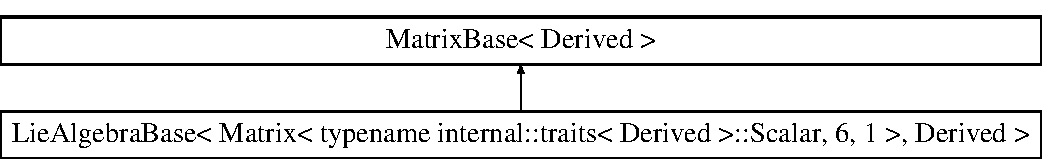
\includegraphics[height=2.000000cm]{class_lie_algebra_base_3_01_matrix_3_01typename_01internal_1_1traits_3_01_derived_01_4_1_1_scala449314c781550590437697c4dc21a6d4}
\end{center}
\end{figure}
\subsection*{Public Types}
\begin{DoxyCompactItemize}
\item 
typedef Matrix$<$ Scalar, 6, 1 $>$ \hyperlink{class_lie_algebra_base_3_01_matrix_3_01typename_01internal_1_1traits_3_01_derived_01_4_1_1_scala449314c781550590437697c4dc21a6d4_abb811fe29a9ece0ee6f2239f17fea23f}{Base\+Type}
\item 
typedef internal\+::traits$<$ Derived $>$\+::\hyperlink{class_lie_algebra_base_3_01_matrix_3_01typename_01internal_1_1traits_3_01_derived_01_4_1_1_scala449314c781550590437697c4dc21a6d4_a52a52c9b33e2ec0441866069e20473ab}{Coefficients} \hyperlink{class_lie_algebra_base_3_01_matrix_3_01typename_01internal_1_1traits_3_01_derived_01_4_1_1_scala449314c781550590437697c4dc21a6d4_a52a52c9b33e2ec0441866069e20473ab}{Coefficients}
\item 
typedef \hyperlink{class_lie_algebra}{Lie\+Algebra}$<$ \hyperlink{class_lie_algebra_base_3_01_matrix_3_01typename_01internal_1_1traits_3_01_derived_01_4_1_1_scala449314c781550590437697c4dc21a6d4_abb811fe29a9ece0ee6f2239f17fea23f}{Base\+Type} $>$ \hyperlink{class_lie_algebra_base_3_01_matrix_3_01typename_01internal_1_1traits_3_01_derived_01_4_1_1_scala449314c781550590437697c4dc21a6d4_a7ce4eac189e072d4fddf555084b3d94f}{Plain\+Object}
\item 
typedef \hyperlink{class_lie_algebra_dual}{Lie\+Algebra\+Dual}$<$ \hyperlink{class_lie_algebra_base_3_01_matrix_3_01typename_01internal_1_1traits_3_01_derived_01_4_1_1_scala449314c781550590437697c4dc21a6d4_abb811fe29a9ece0ee6f2239f17fea23f}{Base\+Type} $>$ \hyperlink{class_lie_algebra_base_3_01_matrix_3_01typename_01internal_1_1traits_3_01_derived_01_4_1_1_scala449314c781550590437697c4dc21a6d4_abdcc3b581461214bd08505af9fbd25d8}{Algebra\+Dual}
\item 
typedef internal\+::traits$<$ Derived $>$\+::\hyperlink{class_lie_algebra_base_3_01_matrix_3_01typename_01internal_1_1traits_3_01_derived_01_4_1_1_scala449314c781550590437697c4dc21a6d4_a578d3791e63ec84b43491f4487f0dffa}{Group} \hyperlink{class_lie_algebra_base_3_01_matrix_3_01typename_01internal_1_1traits_3_01_derived_01_4_1_1_scala449314c781550590437697c4dc21a6d4_a578d3791e63ec84b43491f4487f0dffa}{Group}
\item 
typedef Matrix$<$ Scalar, 6, 6 $>$ \hyperlink{class_lie_algebra_base_3_01_matrix_3_01typename_01internal_1_1traits_3_01_derived_01_4_1_1_scala449314c781550590437697c4dc21a6d4_a01017b6c40956a8cacff4ab187a1bf76}{Matrix6}
\item 
typedef Matrix$<$ Scalar, 3, 1 $>$ \hyperlink{class_lie_algebra_base_3_01_matrix_3_01typename_01internal_1_1traits_3_01_derived_01_4_1_1_scala449314c781550590437697c4dc21a6d4_a18592115cf68b8c745a44d07305df4d2}{Vector3}
\item 
typedef \hyperlink{class_lie_algebra}{Lie\+Algebra}$<$ Matrix$<$ Scalar, 3, 1 $>$ $>$ \hyperlink{class_lie_algebra_base_3_01_matrix_3_01typename_01internal_1_1traits_3_01_derived_01_4_1_1_scala449314c781550590437697c4dc21a6d4_aee714752364bcba43e97f130091fcc6e}{so3\+Element}
\end{DoxyCompactItemize}
\subsection*{Public Member Functions}
\begin{DoxyCompactItemize}
\item 
E\+I\+G\+E\+N\+\_\+\+S\+T\+R\+O\+N\+G\+\_\+\+I\+N\+L\+I\+NE \hyperlink{class_lie_algebra_base}{Lie\+Algebra\+Base} \& \hyperlink{class_lie_algebra_base_3_01_matrix_3_01typename_01internal_1_1traits_3_01_derived_01_4_1_1_scala449314c781550590437697c4dc21a6d4_aac0fa5e5bf38aae42e97aab8c6a13502}{operator=} (const \hyperlink{class_lie_algebra_base}{Lie\+Algebra\+Base} \&other)
\item 
{\footnotesize template$<$class Other\+Derived $>$ }\\E\+I\+G\+E\+N\+\_\+\+S\+T\+R\+O\+N\+G\+\_\+\+I\+N\+L\+I\+NE Derived \& \hyperlink{class_lie_algebra_base_3_01_matrix_3_01typename_01internal_1_1traits_3_01_derived_01_4_1_1_scala449314c781550590437697c4dc21a6d4_a181050e82398e48f0e7d171cdaa899d6}{operator=} (const Matrix\+Base$<$ Other\+Derived $>$ \&other)
\item 
{\footnotesize template$<$class Other\+Derived $>$ }\\\hyperlink{class_lie_algebra_base_3_01_matrix_3_01typename_01internal_1_1traits_3_01_derived_01_4_1_1_scala449314c781550590437697c4dc21a6d4_a7ce4eac189e072d4fddf555084b3d94f}{Plain\+Object} \hyperlink{class_lie_algebra_base_3_01_matrix_3_01typename_01internal_1_1traits_3_01_derived_01_4_1_1_scala449314c781550590437697c4dc21a6d4_a2ffbd92d09b85564bb06712ca119260c}{bracket} (const \hyperlink{class_lie_algebra_base}{Lie\+Algebra\+Base}$<$ \hyperlink{class_lie_algebra_base_3_01_matrix_3_01typename_01internal_1_1traits_3_01_derived_01_4_1_1_scala449314c781550590437697c4dc21a6d4_abb811fe29a9ece0ee6f2239f17fea23f}{Base\+Type}, Other\+Derived $>$ \&a) const
\item 
\hyperlink{class_lie_algebra_base_3_01_matrix_3_01typename_01internal_1_1traits_3_01_derived_01_4_1_1_scala449314c781550590437697c4dc21a6d4_a578d3791e63ec84b43491f4487f0dffa}{Group} \hyperlink{class_lie_algebra_base_3_01_matrix_3_01typename_01internal_1_1traits_3_01_derived_01_4_1_1_scala449314c781550590437697c4dc21a6d4_a7ad2d9384139b52f329ea8d5b836d6b1}{exp} (const Scalar precision=1.e-\/6) const
\item 
Matrix$<$ Scalar, 6, 6 $>$ \hyperlink{class_lie_algebra_base_3_01_matrix_3_01typename_01internal_1_1traits_3_01_derived_01_4_1_1_scala449314c781550590437697c4dc21a6d4_a051939fa1d57d1033430044d337cfaf1}{dexp} () const
\item 
Map$<$ \hyperlink{class_lie_algebra_base_3_01_matrix_3_01typename_01internal_1_1traits_3_01_derived_01_4_1_1_scala449314c781550590437697c4dc21a6d4_aee714752364bcba43e97f130091fcc6e}{so3\+Element} $>$ \hyperlink{class_lie_algebra_base_3_01_matrix_3_01typename_01internal_1_1traits_3_01_derived_01_4_1_1_scala449314c781550590437697c4dc21a6d4_a3b744e47da7a539a3689498fa473feb0}{getso3\+Element} ()
\item 
Map$<$ const \hyperlink{class_lie_algebra_base_3_01_matrix_3_01typename_01internal_1_1traits_3_01_derived_01_4_1_1_scala449314c781550590437697c4dc21a6d4_aee714752364bcba43e97f130091fcc6e}{so3\+Element} $>$ \hyperlink{class_lie_algebra_base_3_01_matrix_3_01typename_01internal_1_1traits_3_01_derived_01_4_1_1_scala449314c781550590437697c4dc21a6d4_a5ea80dc504dc702739a6e8020d503fb7}{getso3\+Element} () const
\item 
Map$<$ \hyperlink{class_lie_algebra_base_3_01_matrix_3_01typename_01internal_1_1traits_3_01_derived_01_4_1_1_scala449314c781550590437697c4dc21a6d4_a18592115cf68b8c745a44d07305df4d2}{Vector3} $>$ \hyperlink{class_lie_algebra_base_3_01_matrix_3_01typename_01internal_1_1traits_3_01_derived_01_4_1_1_scala449314c781550590437697c4dc21a6d4_a1a16f29f03151536b75f66e9f39da843}{get\+R3\+Element} ()
\item 
Map$<$ const \hyperlink{class_lie_algebra_base_3_01_matrix_3_01typename_01internal_1_1traits_3_01_derived_01_4_1_1_scala449314c781550590437697c4dc21a6d4_a18592115cf68b8c745a44d07305df4d2}{Vector3} $>$ \hyperlink{class_lie_algebra_base_3_01_matrix_3_01typename_01internal_1_1traits_3_01_derived_01_4_1_1_scala449314c781550590437697c4dc21a6d4_a12558704431a4884ea9c81a7c6e1d59e}{get\+R3\+Element} () const
\item 
\hyperlink{class_lie_algebra_base_3_01_matrix_3_01typename_01internal_1_1traits_3_01_derived_01_4_1_1_scala449314c781550590437697c4dc21a6d4_a52a52c9b33e2ec0441866069e20473ab}{Coefficients} \& \hyperlink{class_lie_algebra_base_3_01_matrix_3_01typename_01internal_1_1traits_3_01_derived_01_4_1_1_scala449314c781550590437697c4dc21a6d4_a16d1e0fff92a2179f8cb4c7f86a0db64}{get} ()
\item 
const \hyperlink{class_lie_algebra_base_3_01_matrix_3_01typename_01internal_1_1traits_3_01_derived_01_4_1_1_scala449314c781550590437697c4dc21a6d4_a52a52c9b33e2ec0441866069e20473ab}{Coefficients} \& \hyperlink{class_lie_algebra_base_3_01_matrix_3_01typename_01internal_1_1traits_3_01_derived_01_4_1_1_scala449314c781550590437697c4dc21a6d4_add126cad0fccea8e1b14c086232a6544}{get} () const
\item 
{\footnotesize template$<$class Other\+Derived $>$ }\\Derived \& \hyperlink{class_lie_algebra_base_3_01_matrix_3_01typename_01internal_1_1traits_3_01_derived_01_4_1_1_scala449314c781550590437697c4dc21a6d4_a52f06f5362f72159f491b169de48db27}{operator=} (const Matrix\+Base$<$ Other\+Derived $>$ \&other)
\end{DoxyCompactItemize}
\subsection*{Protected Types}
\begin{DoxyCompactItemize}
\item 
typedef Matrix\+Base$<$ Derived $>$ \hyperlink{class_lie_algebra_base_3_01_matrix_3_01typename_01internal_1_1traits_3_01_derived_01_4_1_1_scala449314c781550590437697c4dc21a6d4_a0ab68a3ff4a7f5f7b3682db1dde89651}{Base}
\end{DoxyCompactItemize}


\subsection{Detailed Description}
\subsubsection*{template$<$class Derived$>$\newline
class Lie\+Algebra\+Base$<$ Matrix$<$ typename internal\+::traits$<$ Derived $>$\+::\+Scalar, 6, 1 $>$, Derived $>$}

Base class for the Lie Algebra se(3). 


\begin{DoxyTemplParams}{Template Parameters}
{\em Derived} & the derived class holding the coefficients which are of type Array$<$\+Scalar, 6, 1$>$ or Map$<$Array$<$\+Scalar, 6, 1$>$ $>$\\
\hline
\end{DoxyTemplParams}
This class actually implements methods form \hyperlink{class_lie_algebra_base}{Lie\+Algebra\+Base} for se(3). Since se(3) is the semi direct product of R$^\wedge$3 and so(3) many operations are performed using directly elements form R$^\wedge$3 or so(3)

a Lie Algebra is also a vector Space (check if it\textquotesingle{}s true in the general case) that\textquotesingle{}s why it\textquotesingle{}s inherited from Matrix\+Base 

Definition at line 29 of file Lie\+Algebra\+\_\+se3.\+h.



\subsection{Member Typedef Documentation}
\hypertarget{class_lie_algebra_base_3_01_matrix_3_01typename_01internal_1_1traits_3_01_derived_01_4_1_1_scala449314c781550590437697c4dc21a6d4_abdcc3b581461214bd08505af9fbd25d8}{}\label{class_lie_algebra_base_3_01_matrix_3_01typename_01internal_1_1traits_3_01_derived_01_4_1_1_scala449314c781550590437697c4dc21a6d4_abdcc3b581461214bd08505af9fbd25d8} 
\index{Lie\+Algebra\+Base$<$ Matrix$<$ typename internal\+::traits$<$ Derived $>$\+::\+Scalar, 6, 1 $>$, Derived $>$@{Lie\+Algebra\+Base$<$ Matrix$<$ typename internal\+::traits$<$ Derived $>$\+::\+Scalar, 6, 1 $>$, Derived $>$}!Algebra\+Dual@{Algebra\+Dual}}
\index{Algebra\+Dual@{Algebra\+Dual}!Lie\+Algebra\+Base$<$ Matrix$<$ typename internal\+::traits$<$ Derived $>$\+::\+Scalar, 6, 1 $>$, Derived $>$@{Lie\+Algebra\+Base$<$ Matrix$<$ typename internal\+::traits$<$ Derived $>$\+::\+Scalar, 6, 1 $>$, Derived $>$}}
\subsubsection{\texorpdfstring{Algebra\+Dual}{AlgebraDual}}
{\footnotesize\ttfamily template$<$class Derived $>$ \\
typedef \hyperlink{class_lie_algebra_dual}{Lie\+Algebra\+Dual}$<$\hyperlink{class_lie_algebra_base_3_01_matrix_3_01typename_01internal_1_1traits_3_01_derived_01_4_1_1_scala449314c781550590437697c4dc21a6d4_abb811fe29a9ece0ee6f2239f17fea23f}{Base\+Type}$>$ \hyperlink{class_lie_algebra_base}{Lie\+Algebra\+Base}$<$ Matrix$<$ typename internal\+::traits$<$ Derived $>$\+::Scalar, 6, 1 $>$, Derived $>$\+::\hyperlink{class_lie_algebra_base_3_01_matrix_3_01typename_01internal_1_1traits_3_01_derived_01_4_1_1_scala449314c781550590437697c4dc21a6d4_abdcc3b581461214bd08505af9fbd25d8}{Algebra\+Dual}}

The type of the dual Algebra 

Definition at line 50 of file Lie\+Algebra\+\_\+se3.\+h.

\hypertarget{class_lie_algebra_base_3_01_matrix_3_01typename_01internal_1_1traits_3_01_derived_01_4_1_1_scala449314c781550590437697c4dc21a6d4_a0ab68a3ff4a7f5f7b3682db1dde89651}{}\label{class_lie_algebra_base_3_01_matrix_3_01typename_01internal_1_1traits_3_01_derived_01_4_1_1_scala449314c781550590437697c4dc21a6d4_a0ab68a3ff4a7f5f7b3682db1dde89651} 
\index{Lie\+Algebra\+Base$<$ Matrix$<$ typename internal\+::traits$<$ Derived $>$\+::\+Scalar, 6, 1 $>$, Derived $>$@{Lie\+Algebra\+Base$<$ Matrix$<$ typename internal\+::traits$<$ Derived $>$\+::\+Scalar, 6, 1 $>$, Derived $>$}!Base@{Base}}
\index{Base@{Base}!Lie\+Algebra\+Base$<$ Matrix$<$ typename internal\+::traits$<$ Derived $>$\+::\+Scalar, 6, 1 $>$, Derived $>$@{Lie\+Algebra\+Base$<$ Matrix$<$ typename internal\+::traits$<$ Derived $>$\+::\+Scalar, 6, 1 $>$, Derived $>$}}
\subsubsection{\texorpdfstring{Base}{Base}}
{\footnotesize\ttfamily template$<$class Derived $>$ \\
typedef Matrix\+Base$<$Derived$>$ \hyperlink{class_lie_algebra_base}{Lie\+Algebra\+Base}$<$ Matrix$<$ typename internal\+::traits$<$ Derived $>$\+::Scalar, 6, 1 $>$, Derived $>$\+::\hyperlink{class_lie_algebra_base_3_01_matrix_3_01typename_01internal_1_1traits_3_01_derived_01_4_1_1_scala449314c781550590437697c4dc21a6d4_a0ab68a3ff4a7f5f7b3682db1dde89651}{Base}\hspace{0.3cm}{\ttfamily [protected]}}

The inherited class 

Definition at line 34 of file Lie\+Algebra\+\_\+se3.\+h.

\hypertarget{class_lie_algebra_base_3_01_matrix_3_01typename_01internal_1_1traits_3_01_derived_01_4_1_1_scala449314c781550590437697c4dc21a6d4_abb811fe29a9ece0ee6f2239f17fea23f}{}\label{class_lie_algebra_base_3_01_matrix_3_01typename_01internal_1_1traits_3_01_derived_01_4_1_1_scala449314c781550590437697c4dc21a6d4_abb811fe29a9ece0ee6f2239f17fea23f} 
\index{Lie\+Algebra\+Base$<$ Matrix$<$ typename internal\+::traits$<$ Derived $>$\+::\+Scalar, 6, 1 $>$, Derived $>$@{Lie\+Algebra\+Base$<$ Matrix$<$ typename internal\+::traits$<$ Derived $>$\+::\+Scalar, 6, 1 $>$, Derived $>$}!Base\+Type@{Base\+Type}}
\index{Base\+Type@{Base\+Type}!Lie\+Algebra\+Base$<$ Matrix$<$ typename internal\+::traits$<$ Derived $>$\+::\+Scalar, 6, 1 $>$, Derived $>$@{Lie\+Algebra\+Base$<$ Matrix$<$ typename internal\+::traits$<$ Derived $>$\+::\+Scalar, 6, 1 $>$, Derived $>$}}
\subsubsection{\texorpdfstring{Base\+Type}{BaseType}}
{\footnotesize\ttfamily template$<$class Derived $>$ \\
typedef Matrix$<$Scalar, 6, 1$>$ \hyperlink{class_lie_algebra_base}{Lie\+Algebra\+Base}$<$ Matrix$<$ typename internal\+::traits$<$ Derived $>$\+::Scalar, 6, 1 $>$, Derived $>$\+::\hyperlink{class_lie_algebra_base_3_01_matrix_3_01typename_01internal_1_1traits_3_01_derived_01_4_1_1_scala449314c781550590437697c4dc21a6d4_abb811fe29a9ece0ee6f2239f17fea23f}{Base\+Type}}

The wrapped class 

Definition at line 44 of file Lie\+Algebra\+\_\+se3.\+h.

\hypertarget{class_lie_algebra_base_3_01_matrix_3_01typename_01internal_1_1traits_3_01_derived_01_4_1_1_scala449314c781550590437697c4dc21a6d4_a52a52c9b33e2ec0441866069e20473ab}{}\label{class_lie_algebra_base_3_01_matrix_3_01typename_01internal_1_1traits_3_01_derived_01_4_1_1_scala449314c781550590437697c4dc21a6d4_a52a52c9b33e2ec0441866069e20473ab} 
\index{Lie\+Algebra\+Base$<$ Matrix$<$ typename internal\+::traits$<$ Derived $>$\+::\+Scalar, 6, 1 $>$, Derived $>$@{Lie\+Algebra\+Base$<$ Matrix$<$ typename internal\+::traits$<$ Derived $>$\+::\+Scalar, 6, 1 $>$, Derived $>$}!Coefficients@{Coefficients}}
\index{Coefficients@{Coefficients}!Lie\+Algebra\+Base$<$ Matrix$<$ typename internal\+::traits$<$ Derived $>$\+::\+Scalar, 6, 1 $>$, Derived $>$@{Lie\+Algebra\+Base$<$ Matrix$<$ typename internal\+::traits$<$ Derived $>$\+::\+Scalar, 6, 1 $>$, Derived $>$}}
\subsubsection{\texorpdfstring{Coefficients}{Coefficients}}
{\footnotesize\ttfamily template$<$class Derived $>$ \\
typedef internal\+::traits$<$Derived$>$\+::\hyperlink{class_lie_algebra_base_3_01_matrix_3_01typename_01internal_1_1traits_3_01_derived_01_4_1_1_scala449314c781550590437697c4dc21a6d4_a52a52c9b33e2ec0441866069e20473ab}{Coefficients} \hyperlink{class_lie_algebra_base}{Lie\+Algebra\+Base}$<$ Matrix$<$ typename internal\+::traits$<$ Derived $>$\+::Scalar, 6, 1 $>$, Derived $>$\+::\hyperlink{class_lie_algebra_base_3_01_matrix_3_01typename_01internal_1_1traits_3_01_derived_01_4_1_1_scala449314c781550590437697c4dc21a6d4_a52a52c9b33e2ec0441866069e20473ab}{Coefficients}}

The kind of stored coefficients 

Definition at line 46 of file Lie\+Algebra\+\_\+se3.\+h.

\hypertarget{class_lie_algebra_base_3_01_matrix_3_01typename_01internal_1_1traits_3_01_derived_01_4_1_1_scala449314c781550590437697c4dc21a6d4_a578d3791e63ec84b43491f4487f0dffa}{}\label{class_lie_algebra_base_3_01_matrix_3_01typename_01internal_1_1traits_3_01_derived_01_4_1_1_scala449314c781550590437697c4dc21a6d4_a578d3791e63ec84b43491f4487f0dffa} 
\index{Lie\+Algebra\+Base$<$ Matrix$<$ typename internal\+::traits$<$ Derived $>$\+::\+Scalar, 6, 1 $>$, Derived $>$@{Lie\+Algebra\+Base$<$ Matrix$<$ typename internal\+::traits$<$ Derived $>$\+::\+Scalar, 6, 1 $>$, Derived $>$}!Group@{Group}}
\index{Group@{Group}!Lie\+Algebra\+Base$<$ Matrix$<$ typename internal\+::traits$<$ Derived $>$\+::\+Scalar, 6, 1 $>$, Derived $>$@{Lie\+Algebra\+Base$<$ Matrix$<$ typename internal\+::traits$<$ Derived $>$\+::\+Scalar, 6, 1 $>$, Derived $>$}}
\subsubsection{\texorpdfstring{Group}{Group}}
{\footnotesize\ttfamily template$<$class Derived $>$ \\
typedef internal\+::traits$<$Derived$>$\+::\hyperlink{class_lie_algebra_base_3_01_matrix_3_01typename_01internal_1_1traits_3_01_derived_01_4_1_1_scala449314c781550590437697c4dc21a6d4_a578d3791e63ec84b43491f4487f0dffa}{Group} \hyperlink{class_lie_algebra_base}{Lie\+Algebra\+Base}$<$ Matrix$<$ typename internal\+::traits$<$ Derived $>$\+::Scalar, 6, 1 $>$, Derived $>$\+::\hyperlink{class_lie_algebra_base_3_01_matrix_3_01typename_01internal_1_1traits_3_01_derived_01_4_1_1_scala449314c781550590437697c4dc21a6d4_a578d3791e63ec84b43491f4487f0dffa}{Group}}

The type of the associated Lie Group 

Definition at line 52 of file Lie\+Algebra\+\_\+se3.\+h.

\hypertarget{class_lie_algebra_base_3_01_matrix_3_01typename_01internal_1_1traits_3_01_derived_01_4_1_1_scala449314c781550590437697c4dc21a6d4_a01017b6c40956a8cacff4ab187a1bf76}{}\label{class_lie_algebra_base_3_01_matrix_3_01typename_01internal_1_1traits_3_01_derived_01_4_1_1_scala449314c781550590437697c4dc21a6d4_a01017b6c40956a8cacff4ab187a1bf76} 
\index{Lie\+Algebra\+Base$<$ Matrix$<$ typename internal\+::traits$<$ Derived $>$\+::\+Scalar, 6, 1 $>$, Derived $>$@{Lie\+Algebra\+Base$<$ Matrix$<$ typename internal\+::traits$<$ Derived $>$\+::\+Scalar, 6, 1 $>$, Derived $>$}!Matrix6@{Matrix6}}
\index{Matrix6@{Matrix6}!Lie\+Algebra\+Base$<$ Matrix$<$ typename internal\+::traits$<$ Derived $>$\+::\+Scalar, 6, 1 $>$, Derived $>$@{Lie\+Algebra\+Base$<$ Matrix$<$ typename internal\+::traits$<$ Derived $>$\+::\+Scalar, 6, 1 $>$, Derived $>$}}
\subsubsection{\texorpdfstring{Matrix6}{Matrix6}}
{\footnotesize\ttfamily template$<$class Derived $>$ \\
typedef Matrix$<$Scalar, 6, 6$>$ \hyperlink{class_lie_algebra_base}{Lie\+Algebra\+Base}$<$ Matrix$<$ typename internal\+::traits$<$ Derived $>$\+::Scalar, 6, 1 $>$, Derived $>$\+::\hyperlink{class_lie_algebra_base_3_01_matrix_3_01typename_01internal_1_1traits_3_01_derived_01_4_1_1_scala449314c781550590437697c4dc21a6d4_a01017b6c40956a8cacff4ab187a1bf76}{Matrix6}}

The type of the matrix return by derivatives of exp 

Definition at line 54 of file Lie\+Algebra\+\_\+se3.\+h.

\hypertarget{class_lie_algebra_base_3_01_matrix_3_01typename_01internal_1_1traits_3_01_derived_01_4_1_1_scala449314c781550590437697c4dc21a6d4_a7ce4eac189e072d4fddf555084b3d94f}{}\label{class_lie_algebra_base_3_01_matrix_3_01typename_01internal_1_1traits_3_01_derived_01_4_1_1_scala449314c781550590437697c4dc21a6d4_a7ce4eac189e072d4fddf555084b3d94f} 
\index{Lie\+Algebra\+Base$<$ Matrix$<$ typename internal\+::traits$<$ Derived $>$\+::\+Scalar, 6, 1 $>$, Derived $>$@{Lie\+Algebra\+Base$<$ Matrix$<$ typename internal\+::traits$<$ Derived $>$\+::\+Scalar, 6, 1 $>$, Derived $>$}!Plain\+Object@{Plain\+Object}}
\index{Plain\+Object@{Plain\+Object}!Lie\+Algebra\+Base$<$ Matrix$<$ typename internal\+::traits$<$ Derived $>$\+::\+Scalar, 6, 1 $>$, Derived $>$@{Lie\+Algebra\+Base$<$ Matrix$<$ typename internal\+::traits$<$ Derived $>$\+::\+Scalar, 6, 1 $>$, Derived $>$}}
\subsubsection{\texorpdfstring{Plain\+Object}{PlainObject}}
{\footnotesize\ttfamily template$<$class Derived $>$ \\
typedef \hyperlink{class_lie_algebra}{Lie\+Algebra}$<$\hyperlink{class_lie_algebra_base_3_01_matrix_3_01typename_01internal_1_1traits_3_01_derived_01_4_1_1_scala449314c781550590437697c4dc21a6d4_abb811fe29a9ece0ee6f2239f17fea23f}{Base\+Type}$>$ \hyperlink{class_lie_algebra_base}{Lie\+Algebra\+Base}$<$ Matrix$<$ typename internal\+::traits$<$ Derived $>$\+::Scalar, 6, 1 $>$, Derived $>$\+::\hyperlink{class_lie_algebra_base_3_01_matrix_3_01typename_01internal_1_1traits_3_01_derived_01_4_1_1_scala449314c781550590437697c4dc21a6d4_a7ce4eac189e072d4fddf555084b3d94f}{Plain\+Object}}

The plain object returned, while using Map$<$Lie\+Algebra$<$ $>$ $>$ 

Definition at line 48 of file Lie\+Algebra\+\_\+se3.\+h.

\hypertarget{class_lie_algebra_base_3_01_matrix_3_01typename_01internal_1_1traits_3_01_derived_01_4_1_1_scala449314c781550590437697c4dc21a6d4_aee714752364bcba43e97f130091fcc6e}{}\label{class_lie_algebra_base_3_01_matrix_3_01typename_01internal_1_1traits_3_01_derived_01_4_1_1_scala449314c781550590437697c4dc21a6d4_aee714752364bcba43e97f130091fcc6e} 
\index{Lie\+Algebra\+Base$<$ Matrix$<$ typename internal\+::traits$<$ Derived $>$\+::\+Scalar, 6, 1 $>$, Derived $>$@{Lie\+Algebra\+Base$<$ Matrix$<$ typename internal\+::traits$<$ Derived $>$\+::\+Scalar, 6, 1 $>$, Derived $>$}!so3\+Element@{so3\+Element}}
\index{so3\+Element@{so3\+Element}!Lie\+Algebra\+Base$<$ Matrix$<$ typename internal\+::traits$<$ Derived $>$\+::\+Scalar, 6, 1 $>$, Derived $>$@{Lie\+Algebra\+Base$<$ Matrix$<$ typename internal\+::traits$<$ Derived $>$\+::\+Scalar, 6, 1 $>$, Derived $>$}}
\subsubsection{\texorpdfstring{so3\+Element}{so3Element}}
{\footnotesize\ttfamily template$<$class Derived $>$ \\
typedef \hyperlink{class_lie_algebra}{Lie\+Algebra}$<$Matrix$<$Scalar, 3, 1$>$ $>$ \hyperlink{class_lie_algebra_base}{Lie\+Algebra\+Base}$<$ Matrix$<$ typename internal\+::traits$<$ Derived $>$\+::Scalar, 6, 1 $>$, Derived $>$\+::\hyperlink{class_lie_algebra_base_3_01_matrix_3_01typename_01internal_1_1traits_3_01_derived_01_4_1_1_scala449314c781550590437697c4dc21a6d4_aee714752364bcba43e97f130091fcc6e}{so3\+Element}}

The type of an element of so(3) 

Definition at line 59 of file Lie\+Algebra\+\_\+se3.\+h.

\hypertarget{class_lie_algebra_base_3_01_matrix_3_01typename_01internal_1_1traits_3_01_derived_01_4_1_1_scala449314c781550590437697c4dc21a6d4_a18592115cf68b8c745a44d07305df4d2}{}\label{class_lie_algebra_base_3_01_matrix_3_01typename_01internal_1_1traits_3_01_derived_01_4_1_1_scala449314c781550590437697c4dc21a6d4_a18592115cf68b8c745a44d07305df4d2} 
\index{Lie\+Algebra\+Base$<$ Matrix$<$ typename internal\+::traits$<$ Derived $>$\+::\+Scalar, 6, 1 $>$, Derived $>$@{Lie\+Algebra\+Base$<$ Matrix$<$ typename internal\+::traits$<$ Derived $>$\+::\+Scalar, 6, 1 $>$, Derived $>$}!Vector3@{Vector3}}
\index{Vector3@{Vector3}!Lie\+Algebra\+Base$<$ Matrix$<$ typename internal\+::traits$<$ Derived $>$\+::\+Scalar, 6, 1 $>$, Derived $>$@{Lie\+Algebra\+Base$<$ Matrix$<$ typename internal\+::traits$<$ Derived $>$\+::\+Scalar, 6, 1 $>$, Derived $>$}}
\subsubsection{\texorpdfstring{Vector3}{Vector3}}
{\footnotesize\ttfamily template$<$class Derived $>$ \\
typedef Matrix$<$Scalar, 3, 1$>$ \hyperlink{class_lie_algebra_base}{Lie\+Algebra\+Base}$<$ Matrix$<$ typename internal\+::traits$<$ Derived $>$\+::Scalar, 6, 1 $>$, Derived $>$\+::\hyperlink{class_lie_algebra_base_3_01_matrix_3_01typename_01internal_1_1traits_3_01_derived_01_4_1_1_scala449314c781550590437697c4dc21a6d4_a18592115cf68b8c745a44d07305df4d2}{Vector3}}

The type of an element of R$^\wedge$3 

Definition at line 57 of file Lie\+Algebra\+\_\+se3.\+h.



\subsection{Member Function Documentation}
\hypertarget{class_lie_algebra_base_3_01_matrix_3_01typename_01internal_1_1traits_3_01_derived_01_4_1_1_scala449314c781550590437697c4dc21a6d4_a2ffbd92d09b85564bb06712ca119260c}{}\label{class_lie_algebra_base_3_01_matrix_3_01typename_01internal_1_1traits_3_01_derived_01_4_1_1_scala449314c781550590437697c4dc21a6d4_a2ffbd92d09b85564bb06712ca119260c} 
\index{Lie\+Algebra\+Base$<$ Matrix$<$ typename internal\+::traits$<$ Derived $>$\+::\+Scalar, 6, 1 $>$, Derived $>$@{Lie\+Algebra\+Base$<$ Matrix$<$ typename internal\+::traits$<$ Derived $>$\+::\+Scalar, 6, 1 $>$, Derived $>$}!bracket@{bracket}}
\index{bracket@{bracket}!Lie\+Algebra\+Base$<$ Matrix$<$ typename internal\+::traits$<$ Derived $>$\+::\+Scalar, 6, 1 $>$, Derived $>$@{Lie\+Algebra\+Base$<$ Matrix$<$ typename internal\+::traits$<$ Derived $>$\+::\+Scalar, 6, 1 $>$, Derived $>$}}
\subsubsection{\texorpdfstring{bracket()}{bracket()}}
{\footnotesize\ttfamily template$<$class Derived $>$ \\
template$<$class Other\+Derived $>$ \\
\hyperlink{class_lie_algebra_base}{Lie\+Algebra\+Base}$<$ Matrix$<$ typename internal\+::traits$<$ Derived $>$\+::Scalar, 6, 1 $>$, Derived $>$\+::\hyperlink{class_lie_algebra_base_3_01_matrix_3_01typename_01internal_1_1traits_3_01_derived_01_4_1_1_scala449314c781550590437697c4dc21a6d4_a7ce4eac189e072d4fddf555084b3d94f}{Plain\+Object} \hyperlink{class_lie_algebra_base}{Lie\+Algebra\+Base}$<$ Matrix$<$ typename internal\+::traits$<$ Derived $>$\+::Scalar, 6, 1 $>$, Derived $>$\+::bracket (\begin{DoxyParamCaption}\item[{const \hyperlink{class_lie_algebra_base}{Lie\+Algebra\+Base}$<$ \hyperlink{class_lie_algebra_base_3_01_matrix_3_01typename_01internal_1_1traits_3_01_derived_01_4_1_1_scala449314c781550590437697c4dc21a6d4_abb811fe29a9ece0ee6f2239f17fea23f}{Base\+Type}, Other\+Derived $>$ \&}]{a }\end{DoxyParamCaption}) const}

Lie Bracket 

Definition at line 124 of file Lie\+Algebra\+\_\+se3.\+h.

\hypertarget{class_lie_algebra_base_3_01_matrix_3_01typename_01internal_1_1traits_3_01_derived_01_4_1_1_scala449314c781550590437697c4dc21a6d4_a051939fa1d57d1033430044d337cfaf1}{}\label{class_lie_algebra_base_3_01_matrix_3_01typename_01internal_1_1traits_3_01_derived_01_4_1_1_scala449314c781550590437697c4dc21a6d4_a051939fa1d57d1033430044d337cfaf1} 
\index{Lie\+Algebra\+Base$<$ Matrix$<$ typename internal\+::traits$<$ Derived $>$\+::\+Scalar, 6, 1 $>$, Derived $>$@{Lie\+Algebra\+Base$<$ Matrix$<$ typename internal\+::traits$<$ Derived $>$\+::\+Scalar, 6, 1 $>$, Derived $>$}!dexp@{dexp}}
\index{dexp@{dexp}!Lie\+Algebra\+Base$<$ Matrix$<$ typename internal\+::traits$<$ Derived $>$\+::\+Scalar, 6, 1 $>$, Derived $>$@{Lie\+Algebra\+Base$<$ Matrix$<$ typename internal\+::traits$<$ Derived $>$\+::\+Scalar, 6, 1 $>$, Derived $>$}}
\subsubsection{\texorpdfstring{dexp()}{dexp()}}
{\footnotesize\ttfamily template$<$class Derived $>$ \\
\hyperlink{class_lie_algebra_base}{Lie\+Algebra\+Base}$<$ Matrix$<$ typename internal\+::traits$<$ Derived $>$\+::Scalar, 6, 1 $>$, Derived $>$\+::\hyperlink{class_lie_algebra_base_3_01_matrix_3_01typename_01internal_1_1traits_3_01_derived_01_4_1_1_scala449314c781550590437697c4dc21a6d4_a01017b6c40956a8cacff4ab187a1bf76}{Matrix6} \hyperlink{class_lie_algebra_base}{Lie\+Algebra\+Base}$<$ Matrix$<$ typename internal\+::traits$<$ Derived $>$\+::Scalar, 6, 1 $>$, Derived $>$\+::dexp (\begin{DoxyParamCaption}{ }\end{DoxyParamCaption}) const\hspace{0.3cm}{\ttfamily [inline]}}

\begin{DoxyReturn}{Returns}
the first derivative of exp 
\end{DoxyReturn}
\begin{DoxySeeAlso}{See also}
\hyperlink{class_lie_algebra_base_aafe7d43a29d43aed54dd91b3a3a4c9f7}{Lie\+Algebra\+Base\+::exp} 
\end{DoxySeeAlso}


Definition at line 153 of file Lie\+Algebra\+\_\+se3.\+h.

\hypertarget{class_lie_algebra_base_3_01_matrix_3_01typename_01internal_1_1traits_3_01_derived_01_4_1_1_scala449314c781550590437697c4dc21a6d4_a7ad2d9384139b52f329ea8d5b836d6b1}{}\label{class_lie_algebra_base_3_01_matrix_3_01typename_01internal_1_1traits_3_01_derived_01_4_1_1_scala449314c781550590437697c4dc21a6d4_a7ad2d9384139b52f329ea8d5b836d6b1} 
\index{Lie\+Algebra\+Base$<$ Matrix$<$ typename internal\+::traits$<$ Derived $>$\+::\+Scalar, 6, 1 $>$, Derived $>$@{Lie\+Algebra\+Base$<$ Matrix$<$ typename internal\+::traits$<$ Derived $>$\+::\+Scalar, 6, 1 $>$, Derived $>$}!exp@{exp}}
\index{exp@{exp}!Lie\+Algebra\+Base$<$ Matrix$<$ typename internal\+::traits$<$ Derived $>$\+::\+Scalar, 6, 1 $>$, Derived $>$@{Lie\+Algebra\+Base$<$ Matrix$<$ typename internal\+::traits$<$ Derived $>$\+::\+Scalar, 6, 1 $>$, Derived $>$}}
\subsubsection{\texorpdfstring{exp()}{exp()}}
{\footnotesize\ttfamily template$<$class Derived $>$ \\
\hyperlink{class_lie_algebra_base}{Lie\+Algebra\+Base}$<$ Matrix$<$ typename internal\+::traits$<$ Derived $>$\+::Scalar, 6, 1 $>$, Derived $>$\+::\hyperlink{class_lie_algebra_base_3_01_matrix_3_01typename_01internal_1_1traits_3_01_derived_01_4_1_1_scala449314c781550590437697c4dc21a6d4_a578d3791e63ec84b43491f4487f0dffa}{Group} \hyperlink{class_lie_algebra_base}{Lie\+Algebra\+Base}$<$ Matrix$<$ typename internal\+::traits$<$ Derived $>$\+::Scalar, 6, 1 $>$, Derived $>$\+::exp (\begin{DoxyParamCaption}\item[{const Scalar}]{precision = {\ttfamily 1.e-\/6} }\end{DoxyParamCaption}) const\hspace{0.3cm}{\ttfamily [inline]}}

\begin{DoxyReturn}{Returns}
The element of the associated Lie Group through the exponential map 
\end{DoxyReturn}


Definition at line 144 of file Lie\+Algebra\+\_\+se3.\+h.

\hypertarget{class_lie_algebra_base_3_01_matrix_3_01typename_01internal_1_1traits_3_01_derived_01_4_1_1_scala449314c781550590437697c4dc21a6d4_a16d1e0fff92a2179f8cb4c7f86a0db64}{}\label{class_lie_algebra_base_3_01_matrix_3_01typename_01internal_1_1traits_3_01_derived_01_4_1_1_scala449314c781550590437697c4dc21a6d4_a16d1e0fff92a2179f8cb4c7f86a0db64} 
\index{Lie\+Algebra\+Base$<$ Matrix$<$ typename internal\+::traits$<$ Derived $>$\+::\+Scalar, 6, 1 $>$, Derived $>$@{Lie\+Algebra\+Base$<$ Matrix$<$ typename internal\+::traits$<$ Derived $>$\+::\+Scalar, 6, 1 $>$, Derived $>$}!get@{get}}
\index{get@{get}!Lie\+Algebra\+Base$<$ Matrix$<$ typename internal\+::traits$<$ Derived $>$\+::\+Scalar, 6, 1 $>$, Derived $>$@{Lie\+Algebra\+Base$<$ Matrix$<$ typename internal\+::traits$<$ Derived $>$\+::\+Scalar, 6, 1 $>$, Derived $>$}}
\subsubsection{\texorpdfstring{get()}{get()}\hspace{0.1cm}{\footnotesize\ttfamily [1/2]}}
{\footnotesize\ttfamily template$<$class Derived $>$ \\
\hyperlink{class_lie_algebra_base_3_01_matrix_3_01typename_01internal_1_1traits_3_01_derived_01_4_1_1_scala449314c781550590437697c4dc21a6d4_a52a52c9b33e2ec0441866069e20473ab}{Coefficients}\& \hyperlink{class_lie_algebra_base}{Lie\+Algebra\+Base}$<$ Matrix$<$ typename internal\+::traits$<$ Derived $>$\+::Scalar, 6, 1 $>$, Derived $>$\+::get (\begin{DoxyParamCaption}{ }\end{DoxyParamCaption})\hspace{0.3cm}{\ttfamily [inline]}}

\begin{DoxyReturn}{Returns}
The stored coefficients by the derived class 
\end{DoxyReturn}


Definition at line 92 of file Lie\+Algebra\+\_\+se3.\+h.

\hypertarget{class_lie_algebra_base_3_01_matrix_3_01typename_01internal_1_1traits_3_01_derived_01_4_1_1_scala449314c781550590437697c4dc21a6d4_add126cad0fccea8e1b14c086232a6544}{}\label{class_lie_algebra_base_3_01_matrix_3_01typename_01internal_1_1traits_3_01_derived_01_4_1_1_scala449314c781550590437697c4dc21a6d4_add126cad0fccea8e1b14c086232a6544} 
\index{Lie\+Algebra\+Base$<$ Matrix$<$ typename internal\+::traits$<$ Derived $>$\+::\+Scalar, 6, 1 $>$, Derived $>$@{Lie\+Algebra\+Base$<$ Matrix$<$ typename internal\+::traits$<$ Derived $>$\+::\+Scalar, 6, 1 $>$, Derived $>$}!get@{get}}
\index{get@{get}!Lie\+Algebra\+Base$<$ Matrix$<$ typename internal\+::traits$<$ Derived $>$\+::\+Scalar, 6, 1 $>$, Derived $>$@{Lie\+Algebra\+Base$<$ Matrix$<$ typename internal\+::traits$<$ Derived $>$\+::\+Scalar, 6, 1 $>$, Derived $>$}}
\subsubsection{\texorpdfstring{get()}{get()}\hspace{0.1cm}{\footnotesize\ttfamily [2/2]}}
{\footnotesize\ttfamily template$<$class Derived $>$ \\
const \hyperlink{class_lie_algebra_base_3_01_matrix_3_01typename_01internal_1_1traits_3_01_derived_01_4_1_1_scala449314c781550590437697c4dc21a6d4_a52a52c9b33e2ec0441866069e20473ab}{Coefficients}\& \hyperlink{class_lie_algebra_base}{Lie\+Algebra\+Base}$<$ Matrix$<$ typename internal\+::traits$<$ Derived $>$\+::Scalar, 6, 1 $>$, Derived $>$\+::get (\begin{DoxyParamCaption}{ }\end{DoxyParamCaption}) const\hspace{0.3cm}{\ttfamily [inline]}}

\begin{DoxyReturn}{Returns}
The read-\/only access to the stored coefficients by the derived class 
\end{DoxyReturn}


Definition at line 94 of file Lie\+Algebra\+\_\+se3.\+h.

\hypertarget{class_lie_algebra_base_3_01_matrix_3_01typename_01internal_1_1traits_3_01_derived_01_4_1_1_scala449314c781550590437697c4dc21a6d4_a1a16f29f03151536b75f66e9f39da843}{}\label{class_lie_algebra_base_3_01_matrix_3_01typename_01internal_1_1traits_3_01_derived_01_4_1_1_scala449314c781550590437697c4dc21a6d4_a1a16f29f03151536b75f66e9f39da843} 
\index{Lie\+Algebra\+Base$<$ Matrix$<$ typename internal\+::traits$<$ Derived $>$\+::\+Scalar, 6, 1 $>$, Derived $>$@{Lie\+Algebra\+Base$<$ Matrix$<$ typename internal\+::traits$<$ Derived $>$\+::\+Scalar, 6, 1 $>$, Derived $>$}!get\+R3\+Element@{get\+R3\+Element}}
\index{get\+R3\+Element@{get\+R3\+Element}!Lie\+Algebra\+Base$<$ Matrix$<$ typename internal\+::traits$<$ Derived $>$\+::\+Scalar, 6, 1 $>$, Derived $>$@{Lie\+Algebra\+Base$<$ Matrix$<$ typename internal\+::traits$<$ Derived $>$\+::\+Scalar, 6, 1 $>$, Derived $>$}}
\subsubsection{\texorpdfstring{get\+R3\+Element()}{getR3Element()}\hspace{0.1cm}{\footnotesize\ttfamily [1/2]}}
{\footnotesize\ttfamily template$<$class Derived $>$ \\
Map$<$\hyperlink{class_lie_algebra_base_3_01_matrix_3_01typename_01internal_1_1traits_3_01_derived_01_4_1_1_scala449314c781550590437697c4dc21a6d4_a18592115cf68b8c745a44d07305df4d2}{Vector3}$>$ \hyperlink{class_lie_algebra_base}{Lie\+Algebra\+Base}$<$ Matrix$<$ typename internal\+::traits$<$ Derived $>$\+::Scalar, 6, 1 $>$, Derived $>$\+::get\+R3\+Element (\begin{DoxyParamCaption}{ }\end{DoxyParamCaption})\hspace{0.3cm}{\ttfamily [inline]}}

The accessor to the R$^\wedge$3 element 

Definition at line 87 of file Lie\+Algebra\+\_\+se3.\+h.

\hypertarget{class_lie_algebra_base_3_01_matrix_3_01typename_01internal_1_1traits_3_01_derived_01_4_1_1_scala449314c781550590437697c4dc21a6d4_a12558704431a4884ea9c81a7c6e1d59e}{}\label{class_lie_algebra_base_3_01_matrix_3_01typename_01internal_1_1traits_3_01_derived_01_4_1_1_scala449314c781550590437697c4dc21a6d4_a12558704431a4884ea9c81a7c6e1d59e} 
\index{Lie\+Algebra\+Base$<$ Matrix$<$ typename internal\+::traits$<$ Derived $>$\+::\+Scalar, 6, 1 $>$, Derived $>$@{Lie\+Algebra\+Base$<$ Matrix$<$ typename internal\+::traits$<$ Derived $>$\+::\+Scalar, 6, 1 $>$, Derived $>$}!get\+R3\+Element@{get\+R3\+Element}}
\index{get\+R3\+Element@{get\+R3\+Element}!Lie\+Algebra\+Base$<$ Matrix$<$ typename internal\+::traits$<$ Derived $>$\+::\+Scalar, 6, 1 $>$, Derived $>$@{Lie\+Algebra\+Base$<$ Matrix$<$ typename internal\+::traits$<$ Derived $>$\+::\+Scalar, 6, 1 $>$, Derived $>$}}
\subsubsection{\texorpdfstring{get\+R3\+Element()}{getR3Element()}\hspace{0.1cm}{\footnotesize\ttfamily [2/2]}}
{\footnotesize\ttfamily template$<$class Derived $>$ \\
Map$<$const \hyperlink{class_lie_algebra_base_3_01_matrix_3_01typename_01internal_1_1traits_3_01_derived_01_4_1_1_scala449314c781550590437697c4dc21a6d4_a18592115cf68b8c745a44d07305df4d2}{Vector3}$>$ \hyperlink{class_lie_algebra_base}{Lie\+Algebra\+Base}$<$ Matrix$<$ typename internal\+::traits$<$ Derived $>$\+::Scalar, 6, 1 $>$, Derived $>$\+::get\+R3\+Element (\begin{DoxyParamCaption}{ }\end{DoxyParamCaption}) const\hspace{0.3cm}{\ttfamily [inline]}}

The read-\/only accessor to the R$^\wedge$3 element 

Definition at line 89 of file Lie\+Algebra\+\_\+se3.\+h.

\hypertarget{class_lie_algebra_base_3_01_matrix_3_01typename_01internal_1_1traits_3_01_derived_01_4_1_1_scala449314c781550590437697c4dc21a6d4_a3b744e47da7a539a3689498fa473feb0}{}\label{class_lie_algebra_base_3_01_matrix_3_01typename_01internal_1_1traits_3_01_derived_01_4_1_1_scala449314c781550590437697c4dc21a6d4_a3b744e47da7a539a3689498fa473feb0} 
\index{Lie\+Algebra\+Base$<$ Matrix$<$ typename internal\+::traits$<$ Derived $>$\+::\+Scalar, 6, 1 $>$, Derived $>$@{Lie\+Algebra\+Base$<$ Matrix$<$ typename internal\+::traits$<$ Derived $>$\+::\+Scalar, 6, 1 $>$, Derived $>$}!getso3\+Element@{getso3\+Element}}
\index{getso3\+Element@{getso3\+Element}!Lie\+Algebra\+Base$<$ Matrix$<$ typename internal\+::traits$<$ Derived $>$\+::\+Scalar, 6, 1 $>$, Derived $>$@{Lie\+Algebra\+Base$<$ Matrix$<$ typename internal\+::traits$<$ Derived $>$\+::\+Scalar, 6, 1 $>$, Derived $>$}}
\subsubsection{\texorpdfstring{getso3\+Element()}{getso3Element()}\hspace{0.1cm}{\footnotesize\ttfamily [1/2]}}
{\footnotesize\ttfamily template$<$class Derived $>$ \\
Map$<$\hyperlink{class_lie_algebra_base_3_01_matrix_3_01typename_01internal_1_1traits_3_01_derived_01_4_1_1_scala449314c781550590437697c4dc21a6d4_aee714752364bcba43e97f130091fcc6e}{so3\+Element}$>$ \hyperlink{class_lie_algebra_base}{Lie\+Algebra\+Base}$<$ Matrix$<$ typename internal\+::traits$<$ Derived $>$\+::Scalar, 6, 1 $>$, Derived $>$\+::getso3\+Element (\begin{DoxyParamCaption}{ }\end{DoxyParamCaption})\hspace{0.3cm}{\ttfamily [inline]}}

The accessor to the so(3) element 

Definition at line 83 of file Lie\+Algebra\+\_\+se3.\+h.

\hypertarget{class_lie_algebra_base_3_01_matrix_3_01typename_01internal_1_1traits_3_01_derived_01_4_1_1_scala449314c781550590437697c4dc21a6d4_a5ea80dc504dc702739a6e8020d503fb7}{}\label{class_lie_algebra_base_3_01_matrix_3_01typename_01internal_1_1traits_3_01_derived_01_4_1_1_scala449314c781550590437697c4dc21a6d4_a5ea80dc504dc702739a6e8020d503fb7} 
\index{Lie\+Algebra\+Base$<$ Matrix$<$ typename internal\+::traits$<$ Derived $>$\+::\+Scalar, 6, 1 $>$, Derived $>$@{Lie\+Algebra\+Base$<$ Matrix$<$ typename internal\+::traits$<$ Derived $>$\+::\+Scalar, 6, 1 $>$, Derived $>$}!getso3\+Element@{getso3\+Element}}
\index{getso3\+Element@{getso3\+Element}!Lie\+Algebra\+Base$<$ Matrix$<$ typename internal\+::traits$<$ Derived $>$\+::\+Scalar, 6, 1 $>$, Derived $>$@{Lie\+Algebra\+Base$<$ Matrix$<$ typename internal\+::traits$<$ Derived $>$\+::\+Scalar, 6, 1 $>$, Derived $>$}}
\subsubsection{\texorpdfstring{getso3\+Element()}{getso3Element()}\hspace{0.1cm}{\footnotesize\ttfamily [2/2]}}
{\footnotesize\ttfamily template$<$class Derived $>$ \\
Map$<$const \hyperlink{class_lie_algebra_base_3_01_matrix_3_01typename_01internal_1_1traits_3_01_derived_01_4_1_1_scala449314c781550590437697c4dc21a6d4_aee714752364bcba43e97f130091fcc6e}{so3\+Element}$>$ \hyperlink{class_lie_algebra_base}{Lie\+Algebra\+Base}$<$ Matrix$<$ typename internal\+::traits$<$ Derived $>$\+::Scalar, 6, 1 $>$, Derived $>$\+::getso3\+Element (\begin{DoxyParamCaption}{ }\end{DoxyParamCaption}) const\hspace{0.3cm}{\ttfamily [inline]}}

The read-\/only accessor to the so(3) element 

Definition at line 85 of file Lie\+Algebra\+\_\+se3.\+h.

\hypertarget{class_lie_algebra_base_3_01_matrix_3_01typename_01internal_1_1traits_3_01_derived_01_4_1_1_scala449314c781550590437697c4dc21a6d4_aac0fa5e5bf38aae42e97aab8c6a13502}{}\label{class_lie_algebra_base_3_01_matrix_3_01typename_01internal_1_1traits_3_01_derived_01_4_1_1_scala449314c781550590437697c4dc21a6d4_aac0fa5e5bf38aae42e97aab8c6a13502} 
\index{Lie\+Algebra\+Base$<$ Matrix$<$ typename internal\+::traits$<$ Derived $>$\+::\+Scalar, 6, 1 $>$, Derived $>$@{Lie\+Algebra\+Base$<$ Matrix$<$ typename internal\+::traits$<$ Derived $>$\+::\+Scalar, 6, 1 $>$, Derived $>$}!operator=@{operator=}}
\index{operator=@{operator=}!Lie\+Algebra\+Base$<$ Matrix$<$ typename internal\+::traits$<$ Derived $>$\+::\+Scalar, 6, 1 $>$, Derived $>$@{Lie\+Algebra\+Base$<$ Matrix$<$ typename internal\+::traits$<$ Derived $>$\+::\+Scalar, 6, 1 $>$, Derived $>$}}
\subsubsection{\texorpdfstring{operator=()}{operator=()}\hspace{0.1cm}{\footnotesize\ttfamily [1/3]}}
{\footnotesize\ttfamily template$<$class Derived $>$ \\
\hyperlink{class_lie_algebra_base}{Lie\+Algebra\+Base}$<$ Matrix$<$ typename internal\+::traits$<$ Derived $>$\+::Scalar, 6, 1 $>$, Derived $>$ \& \hyperlink{class_lie_algebra_base}{Lie\+Algebra\+Base}$<$ Matrix$<$ typename internal\+::traits$<$ Derived $>$\+::Scalar, 6, 1 $>$, Derived $>$\+::operator= (\begin{DoxyParamCaption}\item[{const \hyperlink{class_lie_algebra_base}{Lie\+Algebra\+Base}$<$ Matrix$<$ typename internal\+::traits$<$ Derived $>$\+::Scalar, 6, 1 $>$, Derived $>$ \&}]{other }\end{DoxyParamCaption})\hspace{0.3cm}{\ttfamily [inline]}}

Default assignement operator 

Definition at line 104 of file Lie\+Algebra\+\_\+se3.\+h.

\hypertarget{class_lie_algebra_base_3_01_matrix_3_01typename_01internal_1_1traits_3_01_derived_01_4_1_1_scala449314c781550590437697c4dc21a6d4_a181050e82398e48f0e7d171cdaa899d6}{}\label{class_lie_algebra_base_3_01_matrix_3_01typename_01internal_1_1traits_3_01_derived_01_4_1_1_scala449314c781550590437697c4dc21a6d4_a181050e82398e48f0e7d171cdaa899d6} 
\index{Lie\+Algebra\+Base$<$ Matrix$<$ typename internal\+::traits$<$ Derived $>$\+::\+Scalar, 6, 1 $>$, Derived $>$@{Lie\+Algebra\+Base$<$ Matrix$<$ typename internal\+::traits$<$ Derived $>$\+::\+Scalar, 6, 1 $>$, Derived $>$}!operator=@{operator=}}
\index{operator=@{operator=}!Lie\+Algebra\+Base$<$ Matrix$<$ typename internal\+::traits$<$ Derived $>$\+::\+Scalar, 6, 1 $>$, Derived $>$@{Lie\+Algebra\+Base$<$ Matrix$<$ typename internal\+::traits$<$ Derived $>$\+::\+Scalar, 6, 1 $>$, Derived $>$}}
\subsubsection{\texorpdfstring{operator=()}{operator=()}\hspace{0.1cm}{\footnotesize\ttfamily [2/3]}}
{\footnotesize\ttfamily template$<$class Derived $>$ \\
template$<$class Other\+Derived $>$ \\
E\+I\+G\+E\+N\+\_\+\+S\+T\+R\+O\+N\+G\+\_\+\+I\+N\+L\+I\+NE Derived\& \hyperlink{class_lie_algebra_base}{Lie\+Algebra\+Base}$<$ Matrix$<$ typename internal\+::traits$<$ Derived $>$\+::Scalar, 6, 1 $>$, Derived $>$\+::operator= (\begin{DoxyParamCaption}\item[{const Matrix\+Base$<$ Other\+Derived $>$ \&}]{other }\end{DoxyParamCaption})}

Assignement operator between derived type \hypertarget{class_lie_algebra_base_3_01_matrix_3_01typename_01internal_1_1traits_3_01_derived_01_4_1_1_scala449314c781550590437697c4dc21a6d4_a52f06f5362f72159f491b169de48db27}{}\label{class_lie_algebra_base_3_01_matrix_3_01typename_01internal_1_1traits_3_01_derived_01_4_1_1_scala449314c781550590437697c4dc21a6d4_a52f06f5362f72159f491b169de48db27} 
\index{Lie\+Algebra\+Base$<$ Matrix$<$ typename internal\+::traits$<$ Derived $>$\+::\+Scalar, 6, 1 $>$, Derived $>$@{Lie\+Algebra\+Base$<$ Matrix$<$ typename internal\+::traits$<$ Derived $>$\+::\+Scalar, 6, 1 $>$, Derived $>$}!operator=@{operator=}}
\index{operator=@{operator=}!Lie\+Algebra\+Base$<$ Matrix$<$ typename internal\+::traits$<$ Derived $>$\+::\+Scalar, 6, 1 $>$, Derived $>$@{Lie\+Algebra\+Base$<$ Matrix$<$ typename internal\+::traits$<$ Derived $>$\+::\+Scalar, 6, 1 $>$, Derived $>$}}
\subsubsection{\texorpdfstring{operator=()}{operator=()}\hspace{0.1cm}{\footnotesize\ttfamily [3/3]}}
{\footnotesize\ttfamily template$<$class Derived $>$ \\
template$<$class Other\+Derived $>$ \\
Derived\& \hyperlink{class_lie_algebra_base}{Lie\+Algebra\+Base}$<$ Matrix$<$ typename internal\+::traits$<$ Derived $>$\+::Scalar, 6, 1 $>$, Derived $>$\+::operator= (\begin{DoxyParamCaption}\item[{const Matrix\+Base$<$ Other\+Derived $>$ \&}]{other }\end{DoxyParamCaption})\hspace{0.3cm}{\ttfamily [inline]}}



Definition at line 113 of file Lie\+Algebra\+\_\+se3.\+h.



The documentation for this class was generated from the following file\+:\begin{DoxyCompactItemize}
\item 
/\+Users/\+Ryan/\+Code/codyco-\/superbuild/libraries/\+Eigen\+Lgsm/unsupported/\+Eigen/src/\+Lgsm/\hyperlink{_lie_algebra__se3_8h}{Lie\+Algebra\+\_\+se3.\+h}\end{DoxyCompactItemize}

\hypertarget{class_lie_algebra_dual}{}\section{Lie\+Algebra\+Dual$<$ A $>$ Class Template Reference}
\label{class_lie_algebra_dual}\index{Lie\+Algebra\+Dual$<$ A $>$@{Lie\+Algebra\+Dual$<$ A $>$}}


Class describing an element of a Lie algebra dual.  




{\ttfamily \#include $<$Lie\+Algebra.\+h$>$}

Inheritance diagram for Lie\+Algebra\+Dual$<$ A $>$\+:\begin{figure}[H]
\begin{center}
\leavevmode
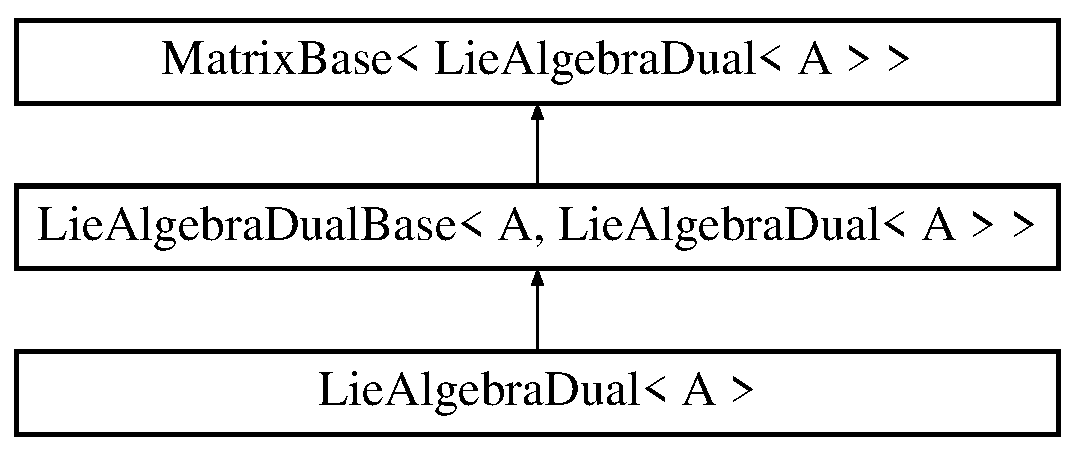
\includegraphics[height=3.000000cm]{class_lie_algebra_dual}
\end{center}
\end{figure}
\subsection*{Public Types}
\begin{DoxyCompactItemize}
\item 
typedef internal\+::traits$<$ \hyperlink{class_lie_algebra_dual}{Lie\+Algebra\+Dual}$<$ A $>$ $>$\+::\hyperlink{class_lie_algebra_dual_a82710c51eb4d0b6cbd190e76a33fbc17}{Coefficients} \hyperlink{class_lie_algebra_dual_a82710c51eb4d0b6cbd190e76a33fbc17}{Coefficients}
\end{DoxyCompactItemize}
\subsection*{Public Member Functions}
\begin{DoxyCompactItemize}
\item 
\hyperlink{class_lie_algebra_dual_a7895f043d19eeee0aba750b83b45da7e}{Lie\+Algebra\+Dual} (const \hyperlink{class_lie_algebra_dual}{Lie\+Algebra\+Dual} \&)
\item 
\hyperlink{class_lie_algebra_dual_a82710c51eb4d0b6cbd190e76a33fbc17}{Coefficients} \& \hyperlink{class_lie_algebra_dual_a9e03668378642cf1147226aa6925a76d}{get} ()
\item 
const \hyperlink{class_lie_algebra_dual_a82710c51eb4d0b6cbd190e76a33fbc17}{Coefficients} \& \hyperlink{class_lie_algebra_dual_aa0fb0278ce57f0ec91b71b849d8e1f3c}{get} () const
\end{DoxyCompactItemize}
\subsection*{Protected Types}
\begin{DoxyCompactItemize}
\item 
typedef \hyperlink{class_lie_algebra_dual_base}{Lie\+Algebra\+Dual\+Base}$<$ A, \hyperlink{class_lie_algebra_dual}{Lie\+Algebra\+Dual}$<$ A $>$ $>$ \hyperlink{class_lie_algebra_dual_ac465396ba89ca481f86d1ce4d4e63a46}{Base}
\end{DoxyCompactItemize}
\subsection*{Protected Attributes}
\begin{DoxyCompactItemize}
\item 
\hyperlink{class_lie_algebra_dual_a82710c51eb4d0b6cbd190e76a33fbc17}{Coefficients} \hyperlink{class_lie_algebra_dual_a14e27002abc8d9b40891ff0f613f0546}{m\+\_\+coeffs}
\end{DoxyCompactItemize}


\subsection{Detailed Description}
\subsubsection*{template$<$class A$>$\newline
class Lie\+Algebra\+Dual$<$ A $>$}

Class describing an element of a Lie algebra dual. 


\begin{DoxyTemplParams}{Template Parameters}
{\em A} & the wrapped class\\
\hline
\end{DoxyTemplParams}
This class must be specialized to add new constructors for a specific algebra dual.

\begin{DoxySeeAlso}{See also}
The methods are defined in \hyperlink{class_lie_algebra_dual_base}{Lie\+Algebra\+Dual\+Base} 
\end{DoxySeeAlso}


Definition at line 216 of file Lie\+Algebra.\+h.



\subsection{Member Typedef Documentation}
\hypertarget{class_lie_algebra_dual_ac465396ba89ca481f86d1ce4d4e63a46}{}\label{class_lie_algebra_dual_ac465396ba89ca481f86d1ce4d4e63a46} 
\index{Lie\+Algebra\+Dual@{Lie\+Algebra\+Dual}!Base@{Base}}
\index{Base@{Base}!Lie\+Algebra\+Dual@{Lie\+Algebra\+Dual}}
\subsubsection{\texorpdfstring{Base}{Base}}
{\footnotesize\ttfamily template$<$class A $>$ \\
typedef \hyperlink{class_lie_algebra_dual_base}{Lie\+Algebra\+Dual\+Base}$<$A, \hyperlink{class_lie_algebra_dual}{Lie\+Algebra\+Dual}$<$A$>$ $>$ \hyperlink{class_lie_algebra_dual}{Lie\+Algebra\+Dual}$<$ A $>$\+::\hyperlink{class_lie_algebra_dual_ac465396ba89ca481f86d1ce4d4e63a46}{Base}\hspace{0.3cm}{\ttfamily [protected]}}



Definition at line 218 of file Lie\+Algebra.\+h.

\hypertarget{class_lie_algebra_dual_a82710c51eb4d0b6cbd190e76a33fbc17}{}\label{class_lie_algebra_dual_a82710c51eb4d0b6cbd190e76a33fbc17} 
\index{Lie\+Algebra\+Dual@{Lie\+Algebra\+Dual}!Coefficients@{Coefficients}}
\index{Coefficients@{Coefficients}!Lie\+Algebra\+Dual@{Lie\+Algebra\+Dual}}
\subsubsection{\texorpdfstring{Coefficients}{Coefficients}}
{\footnotesize\ttfamily template$<$class A $>$ \\
typedef internal\+::traits$<$\hyperlink{class_lie_algebra_dual}{Lie\+Algebra\+Dual}$<$A$>$ $>$\+::\hyperlink{class_lie_algebra_dual_a82710c51eb4d0b6cbd190e76a33fbc17}{Coefficients} \hyperlink{class_lie_algebra_dual}{Lie\+Algebra\+Dual}$<$ A $>$\+::\hyperlink{class_lie_algebra_dual_a82710c51eb4d0b6cbd190e76a33fbc17}{Coefficients}}

Inherited class The stored coefficients 

Definition at line 227 of file Lie\+Algebra.\+h.



\subsection{Constructor \& Destructor Documentation}
\hypertarget{class_lie_algebra_dual_a7895f043d19eeee0aba750b83b45da7e}{}\label{class_lie_algebra_dual_a7895f043d19eeee0aba750b83b45da7e} 
\index{Lie\+Algebra\+Dual@{Lie\+Algebra\+Dual}!Lie\+Algebra\+Dual@{Lie\+Algebra\+Dual}}
\index{Lie\+Algebra\+Dual@{Lie\+Algebra\+Dual}!Lie\+Algebra\+Dual@{Lie\+Algebra\+Dual}}
\subsubsection{\texorpdfstring{Lie\+Algebra\+Dual()}{LieAlgebraDual()}}
{\footnotesize\ttfamily template$<$class A $>$ \\
\hyperlink{class_lie_algebra_dual}{Lie\+Algebra\+Dual}$<$ A $>$\+::\hyperlink{class_lie_algebra_dual}{Lie\+Algebra\+Dual} (\begin{DoxyParamCaption}\item[{const \hyperlink{class_lie_algebra_dual}{Lie\+Algebra\+Dual}$<$ A $>$ \&}]{ }\end{DoxyParamCaption})\hspace{0.3cm}{\ttfamily [inline]}}

Copy constructor \+: do nothing 

\subsection{Member Function Documentation}
\hypertarget{class_lie_algebra_dual_a9e03668378642cf1147226aa6925a76d}{}\label{class_lie_algebra_dual_a9e03668378642cf1147226aa6925a76d} 
\index{Lie\+Algebra\+Dual@{Lie\+Algebra\+Dual}!get@{get}}
\index{get@{get}!Lie\+Algebra\+Dual@{Lie\+Algebra\+Dual}}
\subsubsection{\texorpdfstring{get()}{get()}\hspace{0.1cm}{\footnotesize\ttfamily [1/2]}}
{\footnotesize\ttfamily template$<$class A $>$ \\
\hyperlink{class_lie_algebra_dual_a82710c51eb4d0b6cbd190e76a33fbc17}{Coefficients}\& \hyperlink{class_lie_algebra_dual}{Lie\+Algebra\+Dual}$<$ A $>$\+::get (\begin{DoxyParamCaption}{ }\end{DoxyParamCaption})\hspace{0.3cm}{\ttfamily [inline]}}

\begin{DoxyReturn}{Returns}
The stored coefficients 
\end{DoxyReturn}


Definition at line 233 of file Lie\+Algebra.\+h.

\hypertarget{class_lie_algebra_dual_aa0fb0278ce57f0ec91b71b849d8e1f3c}{}\label{class_lie_algebra_dual_aa0fb0278ce57f0ec91b71b849d8e1f3c} 
\index{Lie\+Algebra\+Dual@{Lie\+Algebra\+Dual}!get@{get}}
\index{get@{get}!Lie\+Algebra\+Dual@{Lie\+Algebra\+Dual}}
\subsubsection{\texorpdfstring{get()}{get()}\hspace{0.1cm}{\footnotesize\ttfamily [2/2]}}
{\footnotesize\ttfamily template$<$class A $>$ \\
const \hyperlink{class_lie_algebra_dual_a82710c51eb4d0b6cbd190e76a33fbc17}{Coefficients}\& \hyperlink{class_lie_algebra_dual}{Lie\+Algebra\+Dual}$<$ A $>$\+::get (\begin{DoxyParamCaption}{ }\end{DoxyParamCaption}) const\hspace{0.3cm}{\ttfamily [inline]}}

\begin{DoxyReturn}{Returns}
The read-\/only access to the stored coefficients 
\end{DoxyReturn}


Definition at line 235 of file Lie\+Algebra.\+h.



\subsection{Member Data Documentation}
\hypertarget{class_lie_algebra_dual_a14e27002abc8d9b40891ff0f613f0546}{}\label{class_lie_algebra_dual_a14e27002abc8d9b40891ff0f613f0546} 
\index{Lie\+Algebra\+Dual@{Lie\+Algebra\+Dual}!m\+\_\+coeffs@{m\+\_\+coeffs}}
\index{m\+\_\+coeffs@{m\+\_\+coeffs}!Lie\+Algebra\+Dual@{Lie\+Algebra\+Dual}}
\subsubsection{\texorpdfstring{m\+\_\+coeffs}{m\_coeffs}}
{\footnotesize\ttfamily template$<$class A $>$ \\
\hyperlink{class_lie_algebra_dual_a82710c51eb4d0b6cbd190e76a33fbc17}{Coefficients} \hyperlink{class_lie_algebra_dual}{Lie\+Algebra\+Dual}$<$ A $>$\+::m\+\_\+coeffs\hspace{0.3cm}{\ttfamily [protected]}}

The wrapped coefficients 

Definition at line 238 of file Lie\+Algebra.\+h.



The documentation for this class was generated from the following file\+:\begin{DoxyCompactItemize}
\item 
/\+Users/\+Ryan/\+Code/codyco-\/superbuild/libraries/\+Eigen\+Lgsm/unsupported/\+Eigen/src/\+Lgsm/\hyperlink{_lie_algebra_8h}{Lie\+Algebra.\+h}\end{DoxyCompactItemize}

\hypertarget{class_lie_algebra_dual_3_01_matrix_3_01___scalar_00_013_00_011_01_4_01_4}{}\section{Lie\+Algebra\+Dual$<$ Matrix$<$ \+\_\+\+Scalar, 3, 1 $>$ $>$ Class Template Reference}
\label{class_lie_algebra_dual_3_01_matrix_3_01___scalar_00_013_00_011_01_4_01_4}\index{Lie\+Algebra\+Dual$<$ Matrix$<$ \+\_\+\+Scalar, 3, 1 $>$ $>$@{Lie\+Algebra\+Dual$<$ Matrix$<$ \+\_\+\+Scalar, 3, 1 $>$ $>$}}


{\ttfamily \#include $<$Lie\+Algebra\+\_\+so3.\+h$>$}

Inheritance diagram for Lie\+Algebra\+Dual$<$ Matrix$<$ \+\_\+\+Scalar, 3, 1 $>$ $>$\+:\begin{figure}[H]
\begin{center}
\leavevmode
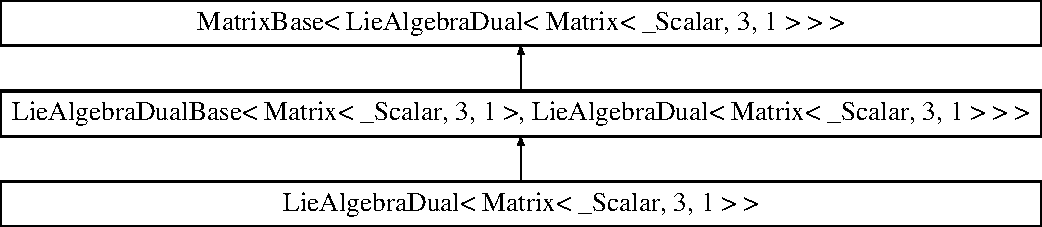
\includegraphics[height=3.000000cm]{class_lie_algebra_dual_3_01_matrix_3_01___scalar_00_013_00_011_01_4_01_4}
\end{center}
\end{figure}
\subsection*{Public Types}
\begin{DoxyCompactItemize}
\item 
typedef internal\+::traits$<$ \hyperlink{class_lie_algebra_dual}{Lie\+Algebra\+Dual}$<$ Matrix$<$ Scalar, 3, 1 $>$ $>$ $>$\+::\hyperlink{class_lie_algebra_dual_3_01_matrix_3_01___scalar_00_013_00_011_01_4_01_4_ae90a3999d66fafefffe5538cd72985ee}{Coefficients} \hyperlink{class_lie_algebra_dual_3_01_matrix_3_01___scalar_00_013_00_011_01_4_01_4_ae90a3999d66fafefffe5538cd72985ee}{Coefficients}
\end{DoxyCompactItemize}
\subsection*{Public Member Functions}
\begin{DoxyCompactItemize}
\item 
\hyperlink{class_lie_algebra_dual_3_01_matrix_3_01___scalar_00_013_00_011_01_4_01_4_a9fa79ebe0f2e3fecd359e63eeb91671a}{Lie\+Algebra\+Dual} ()
\item 
\hyperlink{class_lie_algebra_dual_3_01_matrix_3_01___scalar_00_013_00_011_01_4_01_4_a0f7a068bd94405c6cfc04d3664c5042b}{Lie\+Algebra\+Dual} (const \hyperlink{class_lie_algebra_dual}{Lie\+Algebra\+Dual} \&a)
\item 
\hyperlink{class_lie_algebra_dual_3_01_matrix_3_01___scalar_00_013_00_011_01_4_01_4_ae77a75bc1bef31fa4498c3e4b3888707}{Lie\+Algebra\+Dual} (const \hyperlink{class_lie_algebra_dual_3_01_matrix_3_01___scalar_00_013_00_011_01_4_01_4_ae90a3999d66fafefffe5538cd72985ee}{Coefficients} \&a)
\item 
\hyperlink{class_lie_algebra_dual_3_01_matrix_3_01___scalar_00_013_00_011_01_4_01_4_a6d74b87931ff21cb2a83d32d11a91f27}{Lie\+Algebra\+Dual} (Scalar x, Scalar y, Scalar z)
\item 
\hyperlink{class_lie_algebra_dual_3_01_matrix_3_01___scalar_00_013_00_011_01_4_01_4_ae90a3999d66fafefffe5538cd72985ee}{Coefficients} \& \hyperlink{class_lie_algebra_dual_3_01_matrix_3_01___scalar_00_013_00_011_01_4_01_4_a9bad4e5052a104271c6566e1f9ac3f68}{get} ()
\item 
const \hyperlink{class_lie_algebra_dual_3_01_matrix_3_01___scalar_00_013_00_011_01_4_01_4_ae90a3999d66fafefffe5538cd72985ee}{Coefficients} \& \hyperlink{class_lie_algebra_dual_3_01_matrix_3_01___scalar_00_013_00_011_01_4_01_4_af6625b0911823ad35ae1f5fa23c3d7db}{get} () const
\end{DoxyCompactItemize}
\subsection*{Protected Types}
\begin{DoxyCompactItemize}
\item 
typedef \hyperlink{class_lie_algebra_dual_base}{Lie\+Algebra\+Dual\+Base}$<$ Matrix$<$ \+\_\+\+Scalar, 3, 1 $>$, \hyperlink{class_lie_algebra_dual}{Lie\+Algebra\+Dual}$<$ Matrix$<$ \+\_\+\+Scalar, 3, 1 $>$ $>$ $>$ \hyperlink{class_lie_algebra_dual_3_01_matrix_3_01___scalar_00_013_00_011_01_4_01_4_a32622861071e6634cc868d5e6ec115c7}{Base}
\end{DoxyCompactItemize}
\subsection*{Protected Attributes}
\begin{DoxyCompactItemize}
\item 
\hyperlink{class_lie_algebra_dual_3_01_matrix_3_01___scalar_00_013_00_011_01_4_01_4_ae90a3999d66fafefffe5538cd72985ee}{Coefficients} \hyperlink{class_lie_algebra_dual_3_01_matrix_3_01___scalar_00_013_00_011_01_4_01_4_a85d9fafc5af8ef5b52eb738f5ff191b3}{m\+\_\+coeffs}
\end{DoxyCompactItemize}


\subsection{Detailed Description}
\subsubsection*{template$<$typename \+\_\+\+Scalar$>$\newline
class Lie\+Algebra\+Dual$<$ Matrix$<$ \+\_\+\+Scalar, 3, 1 $>$ $>$}



Definition at line 373 of file Lie\+Algebra\+\_\+so3.\+h.



\subsection{Member Typedef Documentation}
\hypertarget{class_lie_algebra_dual_3_01_matrix_3_01___scalar_00_013_00_011_01_4_01_4_a32622861071e6634cc868d5e6ec115c7}{}\label{class_lie_algebra_dual_3_01_matrix_3_01___scalar_00_013_00_011_01_4_01_4_a32622861071e6634cc868d5e6ec115c7} 
\index{Lie\+Algebra\+Dual$<$ Matrix$<$ \+\_\+\+Scalar, 3, 1 $>$ $>$@{Lie\+Algebra\+Dual$<$ Matrix$<$ \+\_\+\+Scalar, 3, 1 $>$ $>$}!Base@{Base}}
\index{Base@{Base}!Lie\+Algebra\+Dual$<$ Matrix$<$ \+\_\+\+Scalar, 3, 1 $>$ $>$@{Lie\+Algebra\+Dual$<$ Matrix$<$ \+\_\+\+Scalar, 3, 1 $>$ $>$}}
\subsubsection{\texorpdfstring{Base}{Base}}
{\footnotesize\ttfamily template$<$typename \+\_\+\+Scalar $>$ \\
typedef \hyperlink{class_lie_algebra_dual_base}{Lie\+Algebra\+Dual\+Base}$<$Matrix$<$\+\_\+\+Scalar, 3, 1$>$, \hyperlink{class_lie_algebra_dual}{Lie\+Algebra\+Dual}$<$Matrix$<$\+\_\+\+Scalar, 3, 1$>$ $>$ $>$ \hyperlink{class_lie_algebra_dual}{Lie\+Algebra\+Dual}$<$ Matrix$<$ \+\_\+\+Scalar, 3, 1 $>$ $>$\+::\hyperlink{class_lie_algebra_dual_3_01_matrix_3_01___scalar_00_013_00_011_01_4_01_4_a32622861071e6634cc868d5e6ec115c7}{Base}\hspace{0.3cm}{\ttfamily [protected]}}

The inherited class 

Definition at line 378 of file Lie\+Algebra\+\_\+so3.\+h.

\hypertarget{class_lie_algebra_dual_3_01_matrix_3_01___scalar_00_013_00_011_01_4_01_4_ae90a3999d66fafefffe5538cd72985ee}{}\label{class_lie_algebra_dual_3_01_matrix_3_01___scalar_00_013_00_011_01_4_01_4_ae90a3999d66fafefffe5538cd72985ee} 
\index{Lie\+Algebra\+Dual$<$ Matrix$<$ \+\_\+\+Scalar, 3, 1 $>$ $>$@{Lie\+Algebra\+Dual$<$ Matrix$<$ \+\_\+\+Scalar, 3, 1 $>$ $>$}!Coefficients@{Coefficients}}
\index{Coefficients@{Coefficients}!Lie\+Algebra\+Dual$<$ Matrix$<$ \+\_\+\+Scalar, 3, 1 $>$ $>$@{Lie\+Algebra\+Dual$<$ Matrix$<$ \+\_\+\+Scalar, 3, 1 $>$ $>$}}
\subsubsection{\texorpdfstring{Coefficients}{Coefficients}}
{\footnotesize\ttfamily template$<$typename \+\_\+\+Scalar $>$ \\
typedef internal\+::traits$<$\hyperlink{class_lie_algebra_dual}{Lie\+Algebra\+Dual}$<$Matrix$<$Scalar, 3, 1$>$ $>$ $>$\+::\hyperlink{class_lie_algebra_dual_3_01_matrix_3_01___scalar_00_013_00_011_01_4_01_4_ae90a3999d66fafefffe5538cd72985ee}{Coefficients} \hyperlink{class_lie_algebra_dual}{Lie\+Algebra\+Dual}$<$ Matrix$<$ \+\_\+\+Scalar, 3, 1 $>$ $>$\+::\hyperlink{class_lie_algebra_dual_3_01_matrix_3_01___scalar_00_013_00_011_01_4_01_4_ae90a3999d66fafefffe5538cd72985ee}{Coefficients}}

The stored coefficients 

Definition at line 386 of file Lie\+Algebra\+\_\+so3.\+h.



\subsection{Constructor \& Destructor Documentation}
\hypertarget{class_lie_algebra_dual_3_01_matrix_3_01___scalar_00_013_00_011_01_4_01_4_a9fa79ebe0f2e3fecd359e63eeb91671a}{}\label{class_lie_algebra_dual_3_01_matrix_3_01___scalar_00_013_00_011_01_4_01_4_a9fa79ebe0f2e3fecd359e63eeb91671a} 
\index{Lie\+Algebra\+Dual$<$ Matrix$<$ \+\_\+\+Scalar, 3, 1 $>$ $>$@{Lie\+Algebra\+Dual$<$ Matrix$<$ \+\_\+\+Scalar, 3, 1 $>$ $>$}!Lie\+Algebra\+Dual@{Lie\+Algebra\+Dual}}
\index{Lie\+Algebra\+Dual@{Lie\+Algebra\+Dual}!Lie\+Algebra\+Dual$<$ Matrix$<$ \+\_\+\+Scalar, 3, 1 $>$ $>$@{Lie\+Algebra\+Dual$<$ Matrix$<$ \+\_\+\+Scalar, 3, 1 $>$ $>$}}
\subsubsection{\texorpdfstring{Lie\+Algebra\+Dual()}{LieAlgebraDual()}\hspace{0.1cm}{\footnotesize\ttfamily [1/4]}}
{\footnotesize\ttfamily template$<$typename \+\_\+\+Scalar $>$ \\
\hyperlink{class_lie_algebra_dual}{Lie\+Algebra\+Dual}$<$ Matrix$<$ \+\_\+\+Scalar, 3, 1 $>$ $>$\+::\hyperlink{class_lie_algebra_dual}{Lie\+Algebra\+Dual} (\begin{DoxyParamCaption}{ }\end{DoxyParamCaption})\hspace{0.3cm}{\ttfamily [inline]}}

Default constructor 

Definition at line 389 of file Lie\+Algebra\+\_\+so3.\+h.

\hypertarget{class_lie_algebra_dual_3_01_matrix_3_01___scalar_00_013_00_011_01_4_01_4_a0f7a068bd94405c6cfc04d3664c5042b}{}\label{class_lie_algebra_dual_3_01_matrix_3_01___scalar_00_013_00_011_01_4_01_4_a0f7a068bd94405c6cfc04d3664c5042b} 
\index{Lie\+Algebra\+Dual$<$ Matrix$<$ \+\_\+\+Scalar, 3, 1 $>$ $>$@{Lie\+Algebra\+Dual$<$ Matrix$<$ \+\_\+\+Scalar, 3, 1 $>$ $>$}!Lie\+Algebra\+Dual@{Lie\+Algebra\+Dual}}
\index{Lie\+Algebra\+Dual@{Lie\+Algebra\+Dual}!Lie\+Algebra\+Dual$<$ Matrix$<$ \+\_\+\+Scalar, 3, 1 $>$ $>$@{Lie\+Algebra\+Dual$<$ Matrix$<$ \+\_\+\+Scalar, 3, 1 $>$ $>$}}
\subsubsection{\texorpdfstring{Lie\+Algebra\+Dual()}{LieAlgebraDual()}\hspace{0.1cm}{\footnotesize\ttfamily [2/4]}}
{\footnotesize\ttfamily template$<$typename \+\_\+\+Scalar $>$ \\
\hyperlink{class_lie_algebra_dual}{Lie\+Algebra\+Dual}$<$ Matrix$<$ \+\_\+\+Scalar, 3, 1 $>$ $>$\+::\hyperlink{class_lie_algebra_dual}{Lie\+Algebra\+Dual} (\begin{DoxyParamCaption}\item[{const \hyperlink{class_lie_algebra_dual}{Lie\+Algebra\+Dual}$<$ Matrix$<$ \+\_\+\+Scalar, 3, 1 $>$ $>$ \&}]{a }\end{DoxyParamCaption})\hspace{0.3cm}{\ttfamily [inline]}}

Copy constructor 

Definition at line 391 of file Lie\+Algebra\+\_\+so3.\+h.

\hypertarget{class_lie_algebra_dual_3_01_matrix_3_01___scalar_00_013_00_011_01_4_01_4_ae77a75bc1bef31fa4498c3e4b3888707}{}\label{class_lie_algebra_dual_3_01_matrix_3_01___scalar_00_013_00_011_01_4_01_4_ae77a75bc1bef31fa4498c3e4b3888707} 
\index{Lie\+Algebra\+Dual$<$ Matrix$<$ \+\_\+\+Scalar, 3, 1 $>$ $>$@{Lie\+Algebra\+Dual$<$ Matrix$<$ \+\_\+\+Scalar, 3, 1 $>$ $>$}!Lie\+Algebra\+Dual@{Lie\+Algebra\+Dual}}
\index{Lie\+Algebra\+Dual@{Lie\+Algebra\+Dual}!Lie\+Algebra\+Dual$<$ Matrix$<$ \+\_\+\+Scalar, 3, 1 $>$ $>$@{Lie\+Algebra\+Dual$<$ Matrix$<$ \+\_\+\+Scalar, 3, 1 $>$ $>$}}
\subsubsection{\texorpdfstring{Lie\+Algebra\+Dual()}{LieAlgebraDual()}\hspace{0.1cm}{\footnotesize\ttfamily [3/4]}}
{\footnotesize\ttfamily template$<$typename \+\_\+\+Scalar $>$ \\
\hyperlink{class_lie_algebra_dual}{Lie\+Algebra\+Dual}$<$ Matrix$<$ \+\_\+\+Scalar, 3, 1 $>$ $>$\+::\hyperlink{class_lie_algebra_dual}{Lie\+Algebra\+Dual} (\begin{DoxyParamCaption}\item[{const \hyperlink{class_lie_algebra_dual_3_01_matrix_3_01___scalar_00_013_00_011_01_4_01_4_ae90a3999d66fafefffe5538cd72985ee}{Coefficients} \&}]{a }\end{DoxyParamCaption})\hspace{0.3cm}{\ttfamily [inline]}}

Copy constructor 

Definition at line 393 of file Lie\+Algebra\+\_\+so3.\+h.

\hypertarget{class_lie_algebra_dual_3_01_matrix_3_01___scalar_00_013_00_011_01_4_01_4_a6d74b87931ff21cb2a83d32d11a91f27}{}\label{class_lie_algebra_dual_3_01_matrix_3_01___scalar_00_013_00_011_01_4_01_4_a6d74b87931ff21cb2a83d32d11a91f27} 
\index{Lie\+Algebra\+Dual$<$ Matrix$<$ \+\_\+\+Scalar, 3, 1 $>$ $>$@{Lie\+Algebra\+Dual$<$ Matrix$<$ \+\_\+\+Scalar, 3, 1 $>$ $>$}!Lie\+Algebra\+Dual@{Lie\+Algebra\+Dual}}
\index{Lie\+Algebra\+Dual@{Lie\+Algebra\+Dual}!Lie\+Algebra\+Dual$<$ Matrix$<$ \+\_\+\+Scalar, 3, 1 $>$ $>$@{Lie\+Algebra\+Dual$<$ Matrix$<$ \+\_\+\+Scalar, 3, 1 $>$ $>$}}
\subsubsection{\texorpdfstring{Lie\+Algebra\+Dual()}{LieAlgebraDual()}\hspace{0.1cm}{\footnotesize\ttfamily [4/4]}}
{\footnotesize\ttfamily template$<$typename \+\_\+\+Scalar $>$ \\
\hyperlink{class_lie_algebra_dual}{Lie\+Algebra\+Dual}$<$ Matrix$<$ \+\_\+\+Scalar, 3, 1 $>$ $>$\+::\hyperlink{class_lie_algebra_dual}{Lie\+Algebra\+Dual} (\begin{DoxyParamCaption}\item[{Scalar}]{x,  }\item[{Scalar}]{y,  }\item[{Scalar}]{z }\end{DoxyParamCaption})\hspace{0.3cm}{\ttfamily [inline]}}

Constructs an element of so(3) from 3 scalar {\ttfamily x} {\ttfamily y} {\ttfamily z} 

Definition at line 395 of file Lie\+Algebra\+\_\+so3.\+h.



\subsection{Member Function Documentation}
\hypertarget{class_lie_algebra_dual_3_01_matrix_3_01___scalar_00_013_00_011_01_4_01_4_a9bad4e5052a104271c6566e1f9ac3f68}{}\label{class_lie_algebra_dual_3_01_matrix_3_01___scalar_00_013_00_011_01_4_01_4_a9bad4e5052a104271c6566e1f9ac3f68} 
\index{Lie\+Algebra\+Dual$<$ Matrix$<$ \+\_\+\+Scalar, 3, 1 $>$ $>$@{Lie\+Algebra\+Dual$<$ Matrix$<$ \+\_\+\+Scalar, 3, 1 $>$ $>$}!get@{get}}
\index{get@{get}!Lie\+Algebra\+Dual$<$ Matrix$<$ \+\_\+\+Scalar, 3, 1 $>$ $>$@{Lie\+Algebra\+Dual$<$ Matrix$<$ \+\_\+\+Scalar, 3, 1 $>$ $>$}}
\subsubsection{\texorpdfstring{get()}{get()}\hspace{0.1cm}{\footnotesize\ttfamily [1/2]}}
{\footnotesize\ttfamily template$<$typename \+\_\+\+Scalar $>$ \\
\hyperlink{class_lie_algebra_dual_3_01_matrix_3_01___scalar_00_013_00_011_01_4_01_4_ae90a3999d66fafefffe5538cd72985ee}{Coefficients}\& \hyperlink{class_lie_algebra_dual}{Lie\+Algebra\+Dual}$<$ Matrix$<$ \+\_\+\+Scalar, 3, 1 $>$ $>$\+::get (\begin{DoxyParamCaption}{ }\end{DoxyParamCaption})\hspace{0.3cm}{\ttfamily [inline]}}

\begin{DoxyReturn}{Returns}
The stored coefficients 
\end{DoxyReturn}


Definition at line 398 of file Lie\+Algebra\+\_\+so3.\+h.

\hypertarget{class_lie_algebra_dual_3_01_matrix_3_01___scalar_00_013_00_011_01_4_01_4_af6625b0911823ad35ae1f5fa23c3d7db}{}\label{class_lie_algebra_dual_3_01_matrix_3_01___scalar_00_013_00_011_01_4_01_4_af6625b0911823ad35ae1f5fa23c3d7db} 
\index{Lie\+Algebra\+Dual$<$ Matrix$<$ \+\_\+\+Scalar, 3, 1 $>$ $>$@{Lie\+Algebra\+Dual$<$ Matrix$<$ \+\_\+\+Scalar, 3, 1 $>$ $>$}!get@{get}}
\index{get@{get}!Lie\+Algebra\+Dual$<$ Matrix$<$ \+\_\+\+Scalar, 3, 1 $>$ $>$@{Lie\+Algebra\+Dual$<$ Matrix$<$ \+\_\+\+Scalar, 3, 1 $>$ $>$}}
\subsubsection{\texorpdfstring{get()}{get()}\hspace{0.1cm}{\footnotesize\ttfamily [2/2]}}
{\footnotesize\ttfamily template$<$typename \+\_\+\+Scalar $>$ \\
const \hyperlink{class_lie_algebra_dual_3_01_matrix_3_01___scalar_00_013_00_011_01_4_01_4_ae90a3999d66fafefffe5538cd72985ee}{Coefficients}\& \hyperlink{class_lie_algebra_dual}{Lie\+Algebra\+Dual}$<$ Matrix$<$ \+\_\+\+Scalar, 3, 1 $>$ $>$\+::get (\begin{DoxyParamCaption}{ }\end{DoxyParamCaption}) const\hspace{0.3cm}{\ttfamily [inline]}}

\begin{DoxyReturn}{Returns}
The read-\/only access to the stored coefficients 
\end{DoxyReturn}


Definition at line 400 of file Lie\+Algebra\+\_\+so3.\+h.



\subsection{Member Data Documentation}
\hypertarget{class_lie_algebra_dual_3_01_matrix_3_01___scalar_00_013_00_011_01_4_01_4_a85d9fafc5af8ef5b52eb738f5ff191b3}{}\label{class_lie_algebra_dual_3_01_matrix_3_01___scalar_00_013_00_011_01_4_01_4_a85d9fafc5af8ef5b52eb738f5ff191b3} 
\index{Lie\+Algebra\+Dual$<$ Matrix$<$ \+\_\+\+Scalar, 3, 1 $>$ $>$@{Lie\+Algebra\+Dual$<$ Matrix$<$ \+\_\+\+Scalar, 3, 1 $>$ $>$}!m\+\_\+coeffs@{m\+\_\+coeffs}}
\index{m\+\_\+coeffs@{m\+\_\+coeffs}!Lie\+Algebra\+Dual$<$ Matrix$<$ \+\_\+\+Scalar, 3, 1 $>$ $>$@{Lie\+Algebra\+Dual$<$ Matrix$<$ \+\_\+\+Scalar, 3, 1 $>$ $>$}}
\subsubsection{\texorpdfstring{m\+\_\+coeffs}{m\_coeffs}}
{\footnotesize\ttfamily template$<$typename \+\_\+\+Scalar $>$ \\
\hyperlink{class_lie_algebra_dual_3_01_matrix_3_01___scalar_00_013_00_011_01_4_01_4_ae90a3999d66fafefffe5538cd72985ee}{Coefficients} \hyperlink{class_lie_algebra_dual}{Lie\+Algebra\+Dual}$<$ Matrix$<$ \+\_\+\+Scalar, 3, 1 $>$ $>$\+::m\+\_\+coeffs\hspace{0.3cm}{\ttfamily [protected]}}

The wrapped coefficients 

Definition at line 404 of file Lie\+Algebra\+\_\+so3.\+h.



The documentation for this class was generated from the following file\+:\begin{DoxyCompactItemize}
\item 
/\+Users/\+Ryan/\+Code/codyco-\/superbuild/libraries/\+Eigen\+Lgsm/unsupported/\+Eigen/src/\+Lgsm/\hyperlink{_lie_algebra__so3_8h}{Lie\+Algebra\+\_\+so3.\+h}\end{DoxyCompactItemize}

\hypertarget{class_lie_algebra_dual_3_01_matrix_3_01___scalar_00_016_00_011_01_4_01_4}{}\section{Lie\+Algebra\+Dual$<$ Matrix$<$ \+\_\+\+Scalar, 6, 1 $>$ $>$ Class Template Reference}
\label{class_lie_algebra_dual_3_01_matrix_3_01___scalar_00_016_00_011_01_4_01_4}\index{Lie\+Algebra\+Dual$<$ Matrix$<$ \+\_\+\+Scalar, 6, 1 $>$ $>$@{Lie\+Algebra\+Dual$<$ Matrix$<$ \+\_\+\+Scalar, 6, 1 $>$ $>$}}


Class for the se$\ast$(3) Lie algebra dual.  




{\ttfamily \#include $<$Lie\+Algebra\+\_\+se3.\+h$>$}

Inheritance diagram for Lie\+Algebra\+Dual$<$ Matrix$<$ \+\_\+\+Scalar, 6, 1 $>$ $>$\+:\begin{figure}[H]
\begin{center}
\leavevmode
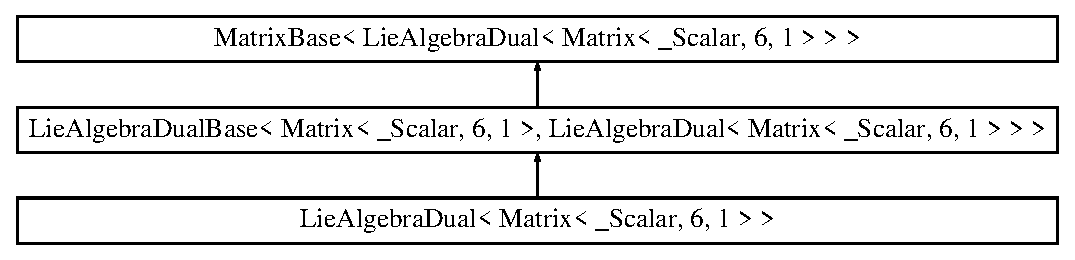
\includegraphics[height=3.000000cm]{class_lie_algebra_dual_3_01_matrix_3_01___scalar_00_016_00_011_01_4_01_4}
\end{center}
\end{figure}
\subsection*{Public Types}
\begin{DoxyCompactItemize}
\item 
typedef internal\+::traits$<$ \hyperlink{class_lie_algebra_dual}{Lie\+Algebra\+Dual}$<$ Matrix$<$ Scalar, 6, 1 $>$ $>$ $>$\+::\hyperlink{class_lie_algebra_dual_3_01_matrix_3_01___scalar_00_016_00_011_01_4_01_4_ae22cd667e4ac77db27cc018db14003bd}{Coefficients} \hyperlink{class_lie_algebra_dual_3_01_matrix_3_01___scalar_00_016_00_011_01_4_01_4_ae22cd667e4ac77db27cc018db14003bd}{Coefficients}
\end{DoxyCompactItemize}
\subsection*{Public Member Functions}
\begin{DoxyCompactItemize}
\item 
\hyperlink{class_lie_algebra_dual_3_01_matrix_3_01___scalar_00_016_00_011_01_4_01_4_a1b04b5f4e09a023256b0056877daac46}{Lie\+Algebra\+Dual} ()
\item 
\hyperlink{class_lie_algebra_dual_3_01_matrix_3_01___scalar_00_016_00_011_01_4_01_4_a798a3a9d717849210ee5d393edf85646}{Lie\+Algebra\+Dual} (const \hyperlink{class_lie_algebra_dual}{Lie\+Algebra\+Dual} \&g)
\item 
\hyperlink{class_lie_algebra_dual_3_01_matrix_3_01___scalar_00_016_00_011_01_4_01_4_a6250264c65f7681975a5683570e258e1}{Lie\+Algebra\+Dual} (const Matrix$<$ Scalar, 6, 1 $>$ \&g)
\item 
\hyperlink{class_lie_algebra_dual_3_01_matrix_3_01___scalar_00_016_00_011_01_4_01_4_a61842ce986294ff68257c54e8ebe6e9f}{Lie\+Algebra\+Dual} (Scalar rx, Scalar ry, Scalar rz, Scalar vx, Scalar vy, Scalar vz)
\item 
\hyperlink{class_lie_algebra_dual_3_01_matrix_3_01___scalar_00_016_00_011_01_4_01_4_ae16baa5a11793aa9621e8d72383834fe}{Lie\+Algebra\+Dual} (const typename Base\+::so3\+Element \&r, const typename Base\+::\+Vector3 \&v)
\item 
\hyperlink{class_lie_algebra_dual_3_01_matrix_3_01___scalar_00_016_00_011_01_4_01_4_ae22cd667e4ac77db27cc018db14003bd}{Coefficients} \& \hyperlink{class_lie_algebra_dual_3_01_matrix_3_01___scalar_00_016_00_011_01_4_01_4_a4ec6e6c98b92fd7f55e065cc122ddcfc}{get} ()
\item 
const \hyperlink{class_lie_algebra_dual_3_01_matrix_3_01___scalar_00_016_00_011_01_4_01_4_ae22cd667e4ac77db27cc018db14003bd}{Coefficients} \& \hyperlink{class_lie_algebra_dual_3_01_matrix_3_01___scalar_00_016_00_011_01_4_01_4_ae618e2d8cc6c4f7bcfa1b237b1dd7654}{get} () const
\end{DoxyCompactItemize}
\subsection*{Protected Types}
\begin{DoxyCompactItemize}
\item 
typedef \hyperlink{class_lie_algebra_dual_base}{Lie\+Algebra\+Dual\+Base}$<$ Matrix$<$ \+\_\+\+Scalar, 6, 1 $>$, \hyperlink{class_lie_algebra_dual}{Lie\+Algebra\+Dual}$<$ Matrix$<$ \+\_\+\+Scalar, 6, 1 $>$ $>$ $>$ \hyperlink{class_lie_algebra_dual_3_01_matrix_3_01___scalar_00_016_00_011_01_4_01_4_a45aa12118237d9a3de26fc61791f31bf}{Base}
\end{DoxyCompactItemize}
\subsection*{Protected Attributes}
\begin{DoxyCompactItemize}
\item 
\hyperlink{class_lie_algebra_dual_3_01_matrix_3_01___scalar_00_016_00_011_01_4_01_4_ae22cd667e4ac77db27cc018db14003bd}{Coefficients} \hyperlink{class_lie_algebra_dual_3_01_matrix_3_01___scalar_00_016_00_011_01_4_01_4_aa6732bb98b628f1d58e95e50f4596b49}{m\+\_\+coeffs}
\end{DoxyCompactItemize}


\subsection{Detailed Description}
\subsubsection*{template$<$typename \+\_\+\+Scalar$>$\newline
class Lie\+Algebra\+Dual$<$ Matrix$<$ \+\_\+\+Scalar, 6, 1 $>$ $>$}

Class for the se$\ast$(3) Lie algebra dual. 


\begin{DoxyTemplParams}{Template Parameters}
{\em \+\_\+\+Scalar} & the type of the underlying array\\
\hline
\end{DoxyTemplParams}
This class is a specialization of \hyperlink{class_lie_algebra_dual}{Lie\+Algebra\+Dual}. It adds specific constructor for se$\ast$(3).

\begin{DoxySeeAlso}{See also}
The methods are defined in \hyperlink{class_lie_algebra_base}{Lie\+Algebra\+Base} 
\end{DoxySeeAlso}


Definition at line 327 of file Lie\+Algebra\+\_\+se3.\+h.



\subsection{Member Typedef Documentation}
\hypertarget{class_lie_algebra_dual_3_01_matrix_3_01___scalar_00_016_00_011_01_4_01_4_a45aa12118237d9a3de26fc61791f31bf}{}\label{class_lie_algebra_dual_3_01_matrix_3_01___scalar_00_016_00_011_01_4_01_4_a45aa12118237d9a3de26fc61791f31bf} 
\index{Lie\+Algebra\+Dual$<$ Matrix$<$ \+\_\+\+Scalar, 6, 1 $>$ $>$@{Lie\+Algebra\+Dual$<$ Matrix$<$ \+\_\+\+Scalar, 6, 1 $>$ $>$}!Base@{Base}}
\index{Base@{Base}!Lie\+Algebra\+Dual$<$ Matrix$<$ \+\_\+\+Scalar, 6, 1 $>$ $>$@{Lie\+Algebra\+Dual$<$ Matrix$<$ \+\_\+\+Scalar, 6, 1 $>$ $>$}}
\subsubsection{\texorpdfstring{Base}{Base}}
{\footnotesize\ttfamily template$<$typename \+\_\+\+Scalar $>$ \\
typedef \hyperlink{class_lie_algebra_dual_base}{Lie\+Algebra\+Dual\+Base}$<$Matrix$<$\+\_\+\+Scalar, 6, 1$>$, \hyperlink{class_lie_algebra_dual}{Lie\+Algebra\+Dual}$<$Matrix$<$\+\_\+\+Scalar, 6, 1$>$ $>$ $>$ \hyperlink{class_lie_algebra_dual}{Lie\+Algebra\+Dual}$<$ Matrix$<$ \+\_\+\+Scalar, 6, 1 $>$ $>$\+::\hyperlink{class_lie_algebra_dual_3_01_matrix_3_01___scalar_00_016_00_011_01_4_01_4_a45aa12118237d9a3de26fc61791f31bf}{Base}\hspace{0.3cm}{\ttfamily [protected]}}



Definition at line 331 of file Lie\+Algebra\+\_\+se3.\+h.

\hypertarget{class_lie_algebra_dual_3_01_matrix_3_01___scalar_00_016_00_011_01_4_01_4_ae22cd667e4ac77db27cc018db14003bd}{}\label{class_lie_algebra_dual_3_01_matrix_3_01___scalar_00_016_00_011_01_4_01_4_ae22cd667e4ac77db27cc018db14003bd} 
\index{Lie\+Algebra\+Dual$<$ Matrix$<$ \+\_\+\+Scalar, 6, 1 $>$ $>$@{Lie\+Algebra\+Dual$<$ Matrix$<$ \+\_\+\+Scalar, 6, 1 $>$ $>$}!Coefficients@{Coefficients}}
\index{Coefficients@{Coefficients}!Lie\+Algebra\+Dual$<$ Matrix$<$ \+\_\+\+Scalar, 6, 1 $>$ $>$@{Lie\+Algebra\+Dual$<$ Matrix$<$ \+\_\+\+Scalar, 6, 1 $>$ $>$}}
\subsubsection{\texorpdfstring{Coefficients}{Coefficients}}
{\footnotesize\ttfamily template$<$typename \+\_\+\+Scalar $>$ \\
typedef internal\+::traits$<$\hyperlink{class_lie_algebra_dual}{Lie\+Algebra\+Dual}$<$Matrix$<$Scalar, 6, 1$>$ $>$ $>$\+::\hyperlink{class_lie_algebra_dual_3_01_matrix_3_01___scalar_00_016_00_011_01_4_01_4_ae22cd667e4ac77db27cc018db14003bd}{Coefficients} \hyperlink{class_lie_algebra_dual}{Lie\+Algebra\+Dual}$<$ Matrix$<$ \+\_\+\+Scalar, 6, 1 $>$ $>$\+::\hyperlink{class_lie_algebra_dual_3_01_matrix_3_01___scalar_00_016_00_011_01_4_01_4_ae22cd667e4ac77db27cc018db14003bd}{Coefficients}}



Definition at line 338 of file Lie\+Algebra\+\_\+se3.\+h.



\subsection{Constructor \& Destructor Documentation}
\hypertarget{class_lie_algebra_dual_3_01_matrix_3_01___scalar_00_016_00_011_01_4_01_4_a1b04b5f4e09a023256b0056877daac46}{}\label{class_lie_algebra_dual_3_01_matrix_3_01___scalar_00_016_00_011_01_4_01_4_a1b04b5f4e09a023256b0056877daac46} 
\index{Lie\+Algebra\+Dual$<$ Matrix$<$ \+\_\+\+Scalar, 6, 1 $>$ $>$@{Lie\+Algebra\+Dual$<$ Matrix$<$ \+\_\+\+Scalar, 6, 1 $>$ $>$}!Lie\+Algebra\+Dual@{Lie\+Algebra\+Dual}}
\index{Lie\+Algebra\+Dual@{Lie\+Algebra\+Dual}!Lie\+Algebra\+Dual$<$ Matrix$<$ \+\_\+\+Scalar, 6, 1 $>$ $>$@{Lie\+Algebra\+Dual$<$ Matrix$<$ \+\_\+\+Scalar, 6, 1 $>$ $>$}}
\subsubsection{\texorpdfstring{Lie\+Algebra\+Dual()}{LieAlgebraDual()}\hspace{0.1cm}{\footnotesize\ttfamily [1/5]}}
{\footnotesize\ttfamily template$<$typename \+\_\+\+Scalar $>$ \\
\hyperlink{class_lie_algebra_dual}{Lie\+Algebra\+Dual}$<$ Matrix$<$ \+\_\+\+Scalar, 6, 1 $>$ $>$\+::\hyperlink{class_lie_algebra_dual}{Lie\+Algebra\+Dual} (\begin{DoxyParamCaption}{ }\end{DoxyParamCaption})\hspace{0.3cm}{\ttfamily [inline]}}



Definition at line 340 of file Lie\+Algebra\+\_\+se3.\+h.

\hypertarget{class_lie_algebra_dual_3_01_matrix_3_01___scalar_00_016_00_011_01_4_01_4_a798a3a9d717849210ee5d393edf85646}{}\label{class_lie_algebra_dual_3_01_matrix_3_01___scalar_00_016_00_011_01_4_01_4_a798a3a9d717849210ee5d393edf85646} 
\index{Lie\+Algebra\+Dual$<$ Matrix$<$ \+\_\+\+Scalar, 6, 1 $>$ $>$@{Lie\+Algebra\+Dual$<$ Matrix$<$ \+\_\+\+Scalar, 6, 1 $>$ $>$}!Lie\+Algebra\+Dual@{Lie\+Algebra\+Dual}}
\index{Lie\+Algebra\+Dual@{Lie\+Algebra\+Dual}!Lie\+Algebra\+Dual$<$ Matrix$<$ \+\_\+\+Scalar, 6, 1 $>$ $>$@{Lie\+Algebra\+Dual$<$ Matrix$<$ \+\_\+\+Scalar, 6, 1 $>$ $>$}}
\subsubsection{\texorpdfstring{Lie\+Algebra\+Dual()}{LieAlgebraDual()}\hspace{0.1cm}{\footnotesize\ttfamily [2/5]}}
{\footnotesize\ttfamily template$<$typename \+\_\+\+Scalar $>$ \\
\hyperlink{class_lie_algebra_dual}{Lie\+Algebra\+Dual}$<$ Matrix$<$ \+\_\+\+Scalar, 6, 1 $>$ $>$\+::\hyperlink{class_lie_algebra_dual}{Lie\+Algebra\+Dual} (\begin{DoxyParamCaption}\item[{const \hyperlink{class_lie_algebra_dual}{Lie\+Algebra\+Dual}$<$ Matrix$<$ \+\_\+\+Scalar, 6, 1 $>$ $>$ \&}]{g }\end{DoxyParamCaption})\hspace{0.3cm}{\ttfamily [inline]}}



Definition at line 341 of file Lie\+Algebra\+\_\+se3.\+h.

\hypertarget{class_lie_algebra_dual_3_01_matrix_3_01___scalar_00_016_00_011_01_4_01_4_a6250264c65f7681975a5683570e258e1}{}\label{class_lie_algebra_dual_3_01_matrix_3_01___scalar_00_016_00_011_01_4_01_4_a6250264c65f7681975a5683570e258e1} 
\index{Lie\+Algebra\+Dual$<$ Matrix$<$ \+\_\+\+Scalar, 6, 1 $>$ $>$@{Lie\+Algebra\+Dual$<$ Matrix$<$ \+\_\+\+Scalar, 6, 1 $>$ $>$}!Lie\+Algebra\+Dual@{Lie\+Algebra\+Dual}}
\index{Lie\+Algebra\+Dual@{Lie\+Algebra\+Dual}!Lie\+Algebra\+Dual$<$ Matrix$<$ \+\_\+\+Scalar, 6, 1 $>$ $>$@{Lie\+Algebra\+Dual$<$ Matrix$<$ \+\_\+\+Scalar, 6, 1 $>$ $>$}}
\subsubsection{\texorpdfstring{Lie\+Algebra\+Dual()}{LieAlgebraDual()}\hspace{0.1cm}{\footnotesize\ttfamily [3/5]}}
{\footnotesize\ttfamily template$<$typename \+\_\+\+Scalar $>$ \\
\hyperlink{class_lie_algebra_dual}{Lie\+Algebra\+Dual}$<$ Matrix$<$ \+\_\+\+Scalar, 6, 1 $>$ $>$\+::\hyperlink{class_lie_algebra_dual}{Lie\+Algebra\+Dual} (\begin{DoxyParamCaption}\item[{const Matrix$<$ Scalar, 6, 1 $>$ \&}]{g }\end{DoxyParamCaption})\hspace{0.3cm}{\ttfamily [inline]}}



Definition at line 342 of file Lie\+Algebra\+\_\+se3.\+h.

\hypertarget{class_lie_algebra_dual_3_01_matrix_3_01___scalar_00_016_00_011_01_4_01_4_a61842ce986294ff68257c54e8ebe6e9f}{}\label{class_lie_algebra_dual_3_01_matrix_3_01___scalar_00_016_00_011_01_4_01_4_a61842ce986294ff68257c54e8ebe6e9f} 
\index{Lie\+Algebra\+Dual$<$ Matrix$<$ \+\_\+\+Scalar, 6, 1 $>$ $>$@{Lie\+Algebra\+Dual$<$ Matrix$<$ \+\_\+\+Scalar, 6, 1 $>$ $>$}!Lie\+Algebra\+Dual@{Lie\+Algebra\+Dual}}
\index{Lie\+Algebra\+Dual@{Lie\+Algebra\+Dual}!Lie\+Algebra\+Dual$<$ Matrix$<$ \+\_\+\+Scalar, 6, 1 $>$ $>$@{Lie\+Algebra\+Dual$<$ Matrix$<$ \+\_\+\+Scalar, 6, 1 $>$ $>$}}
\subsubsection{\texorpdfstring{Lie\+Algebra\+Dual()}{LieAlgebraDual()}\hspace{0.1cm}{\footnotesize\ttfamily [4/5]}}
{\footnotesize\ttfamily template$<$typename \+\_\+\+Scalar $>$ \\
\hyperlink{class_lie_algebra_dual}{Lie\+Algebra\+Dual}$<$ Matrix$<$ \+\_\+\+Scalar, 6, 1 $>$ $>$\+::\hyperlink{class_lie_algebra_dual}{Lie\+Algebra\+Dual} (\begin{DoxyParamCaption}\item[{Scalar}]{rx,  }\item[{Scalar}]{ry,  }\item[{Scalar}]{rz,  }\item[{Scalar}]{vx,  }\item[{Scalar}]{vy,  }\item[{Scalar}]{vz }\end{DoxyParamCaption})\hspace{0.3cm}{\ttfamily [inline]}}



Definition at line 343 of file Lie\+Algebra\+\_\+se3.\+h.

\hypertarget{class_lie_algebra_dual_3_01_matrix_3_01___scalar_00_016_00_011_01_4_01_4_ae16baa5a11793aa9621e8d72383834fe}{}\label{class_lie_algebra_dual_3_01_matrix_3_01___scalar_00_016_00_011_01_4_01_4_ae16baa5a11793aa9621e8d72383834fe} 
\index{Lie\+Algebra\+Dual$<$ Matrix$<$ \+\_\+\+Scalar, 6, 1 $>$ $>$@{Lie\+Algebra\+Dual$<$ Matrix$<$ \+\_\+\+Scalar, 6, 1 $>$ $>$}!Lie\+Algebra\+Dual@{Lie\+Algebra\+Dual}}
\index{Lie\+Algebra\+Dual@{Lie\+Algebra\+Dual}!Lie\+Algebra\+Dual$<$ Matrix$<$ \+\_\+\+Scalar, 6, 1 $>$ $>$@{Lie\+Algebra\+Dual$<$ Matrix$<$ \+\_\+\+Scalar, 6, 1 $>$ $>$}}
\subsubsection{\texorpdfstring{Lie\+Algebra\+Dual()}{LieAlgebraDual()}\hspace{0.1cm}{\footnotesize\ttfamily [5/5]}}
{\footnotesize\ttfamily template$<$typename \+\_\+\+Scalar $>$ \\
\hyperlink{class_lie_algebra_dual}{Lie\+Algebra\+Dual}$<$ Matrix$<$ \+\_\+\+Scalar, 6, 1 $>$ $>$\+::\hyperlink{class_lie_algebra_dual}{Lie\+Algebra\+Dual} (\begin{DoxyParamCaption}\item[{const typename Base\+::so3\+Element \&}]{r,  }\item[{const typename Base\+::\+Vector3 \&}]{v }\end{DoxyParamCaption})\hspace{0.3cm}{\ttfamily [inline]}}



Definition at line 346 of file Lie\+Algebra\+\_\+se3.\+h.



\subsection{Member Function Documentation}
\hypertarget{class_lie_algebra_dual_3_01_matrix_3_01___scalar_00_016_00_011_01_4_01_4_a4ec6e6c98b92fd7f55e065cc122ddcfc}{}\label{class_lie_algebra_dual_3_01_matrix_3_01___scalar_00_016_00_011_01_4_01_4_a4ec6e6c98b92fd7f55e065cc122ddcfc} 
\index{Lie\+Algebra\+Dual$<$ Matrix$<$ \+\_\+\+Scalar, 6, 1 $>$ $>$@{Lie\+Algebra\+Dual$<$ Matrix$<$ \+\_\+\+Scalar, 6, 1 $>$ $>$}!get@{get}}
\index{get@{get}!Lie\+Algebra\+Dual$<$ Matrix$<$ \+\_\+\+Scalar, 6, 1 $>$ $>$@{Lie\+Algebra\+Dual$<$ Matrix$<$ \+\_\+\+Scalar, 6, 1 $>$ $>$}}
\subsubsection{\texorpdfstring{get()}{get()}\hspace{0.1cm}{\footnotesize\ttfamily [1/2]}}
{\footnotesize\ttfamily template$<$typename \+\_\+\+Scalar $>$ \\
\hyperlink{class_lie_algebra_dual_3_01_matrix_3_01___scalar_00_016_00_011_01_4_01_4_ae22cd667e4ac77db27cc018db14003bd}{Coefficients}\& \hyperlink{class_lie_algebra_dual}{Lie\+Algebra\+Dual}$<$ Matrix$<$ \+\_\+\+Scalar, 6, 1 $>$ $>$\+::get (\begin{DoxyParamCaption}{ }\end{DoxyParamCaption})\hspace{0.3cm}{\ttfamily [inline]}}



Definition at line 351 of file Lie\+Algebra\+\_\+se3.\+h.

\hypertarget{class_lie_algebra_dual_3_01_matrix_3_01___scalar_00_016_00_011_01_4_01_4_ae618e2d8cc6c4f7bcfa1b237b1dd7654}{}\label{class_lie_algebra_dual_3_01_matrix_3_01___scalar_00_016_00_011_01_4_01_4_ae618e2d8cc6c4f7bcfa1b237b1dd7654} 
\index{Lie\+Algebra\+Dual$<$ Matrix$<$ \+\_\+\+Scalar, 6, 1 $>$ $>$@{Lie\+Algebra\+Dual$<$ Matrix$<$ \+\_\+\+Scalar, 6, 1 $>$ $>$}!get@{get}}
\index{get@{get}!Lie\+Algebra\+Dual$<$ Matrix$<$ \+\_\+\+Scalar, 6, 1 $>$ $>$@{Lie\+Algebra\+Dual$<$ Matrix$<$ \+\_\+\+Scalar, 6, 1 $>$ $>$}}
\subsubsection{\texorpdfstring{get()}{get()}\hspace{0.1cm}{\footnotesize\ttfamily [2/2]}}
{\footnotesize\ttfamily template$<$typename \+\_\+\+Scalar $>$ \\
const \hyperlink{class_lie_algebra_dual_3_01_matrix_3_01___scalar_00_016_00_011_01_4_01_4_ae22cd667e4ac77db27cc018db14003bd}{Coefficients}\& \hyperlink{class_lie_algebra_dual}{Lie\+Algebra\+Dual}$<$ Matrix$<$ \+\_\+\+Scalar, 6, 1 $>$ $>$\+::get (\begin{DoxyParamCaption}{ }\end{DoxyParamCaption}) const\hspace{0.3cm}{\ttfamily [inline]}}



Definition at line 352 of file Lie\+Algebra\+\_\+se3.\+h.



\subsection{Member Data Documentation}
\hypertarget{class_lie_algebra_dual_3_01_matrix_3_01___scalar_00_016_00_011_01_4_01_4_aa6732bb98b628f1d58e95e50f4596b49}{}\label{class_lie_algebra_dual_3_01_matrix_3_01___scalar_00_016_00_011_01_4_01_4_aa6732bb98b628f1d58e95e50f4596b49} 
\index{Lie\+Algebra\+Dual$<$ Matrix$<$ \+\_\+\+Scalar, 6, 1 $>$ $>$@{Lie\+Algebra\+Dual$<$ Matrix$<$ \+\_\+\+Scalar, 6, 1 $>$ $>$}!m\+\_\+coeffs@{m\+\_\+coeffs}}
\index{m\+\_\+coeffs@{m\+\_\+coeffs}!Lie\+Algebra\+Dual$<$ Matrix$<$ \+\_\+\+Scalar, 6, 1 $>$ $>$@{Lie\+Algebra\+Dual$<$ Matrix$<$ \+\_\+\+Scalar, 6, 1 $>$ $>$}}
\subsubsection{\texorpdfstring{m\+\_\+coeffs}{m\_coeffs}}
{\footnotesize\ttfamily template$<$typename \+\_\+\+Scalar $>$ \\
\hyperlink{class_lie_algebra_dual_3_01_matrix_3_01___scalar_00_016_00_011_01_4_01_4_ae22cd667e4ac77db27cc018db14003bd}{Coefficients} \hyperlink{class_lie_algebra_dual}{Lie\+Algebra\+Dual}$<$ Matrix$<$ \+\_\+\+Scalar, 6, 1 $>$ $>$\+::m\+\_\+coeffs\hspace{0.3cm}{\ttfamily [protected]}}



Definition at line 355 of file Lie\+Algebra\+\_\+se3.\+h.



The documentation for this class was generated from the following file\+:\begin{DoxyCompactItemize}
\item 
/\+Users/\+Ryan/\+Code/codyco-\/superbuild/libraries/\+Eigen\+Lgsm/unsupported/\+Eigen/src/\+Lgsm/\hyperlink{_lie_algebra__se3_8h}{Lie\+Algebra\+\_\+se3.\+h}\end{DoxyCompactItemize}

\hypertarget{class_lie_algebra_dual_base}{}\section{Lie\+Algebra\+Dual\+Base$<$ A, Derived $>$ Class Template Reference}
\label{class_lie_algebra_dual_base}\index{Lie\+Algebra\+Dual\+Base$<$ A, Derived $>$@{Lie\+Algebra\+Dual\+Base$<$ A, Derived $>$}}


{\ttfamily \#include $<$Lie\+Algebra.\+h$>$}

Inheritance diagram for Lie\+Algebra\+Dual\+Base$<$ A, Derived $>$\+:\begin{figure}[H]
\begin{center}
\leavevmode
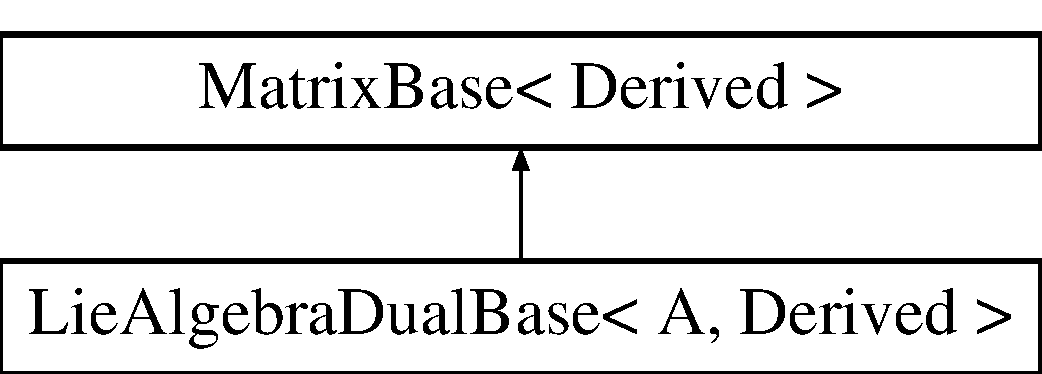
\includegraphics[height=2.000000cm]{class_lie_algebra_dual_base}
\end{center}
\end{figure}
\subsection*{Public Types}
\begin{DoxyCompactItemize}
\item 
typedef A \hyperlink{class_lie_algebra_dual_base_a1d0d10f7479bc0e235b13e29f1c012d2}{Base\+Type}
\item 
typedef internal\+::traits$<$ Derived $>$\+::\hyperlink{class_lie_algebra_dual_base_a9cbdf57fdc61d9ff457e9a9a814f5fdd}{Coefficients} \hyperlink{class_lie_algebra_dual_base_a9cbdf57fdc61d9ff457e9a9a814f5fdd}{Coefficients}
\item 
typedef \hyperlink{class_lie_algebra_dual}{Lie\+Algebra\+Dual}$<$ \hyperlink{class_lie_algebra_dual_base_a1d0d10f7479bc0e235b13e29f1c012d2}{Base\+Type} $>$ \hyperlink{class_lie_algebra_dual_base_a9b59cead2f78ed837cd22a96155e5da3}{Plain\+Object}
\item 
typedef \hyperlink{class_lie_algebra}{Lie\+Algebra}$<$ \hyperlink{class_lie_algebra_dual_base_a1d0d10f7479bc0e235b13e29f1c012d2}{Base\+Type} $>$ \hyperlink{class_lie_algebra_dual_base_a50d4fa9e6b80c63c7ec5955717133db3}{Algebra}
\item 
typedef internal\+::traits$<$ Derived $>$\+::\hyperlink{class_lie_algebra_dual_base_a540618e11addb56f20f6d007204c107c}{Group} \hyperlink{class_lie_algebra_dual_base_a540618e11addb56f20f6d007204c107c}{Group}
\end{DoxyCompactItemize}
\subsection*{Public Member Functions}
\begin{DoxyCompactItemize}
\item 
E\+I\+G\+E\+N\+\_\+\+S\+T\+R\+O\+N\+G\+\_\+\+I\+N\+L\+I\+NE \hyperlink{class_lie_algebra_dual_base}{Lie\+Algebra\+Dual\+Base} \& \hyperlink{class_lie_algebra_dual_base_a849c6b62c74363de84a0979ca7ed42ec}{operator=} (const \hyperlink{class_lie_algebra_dual_base}{Lie\+Algebra\+Dual\+Base} \&other)
\item 
{\footnotesize template$<$class Base\+Type , class Other\+Derived $>$ }\\E\+I\+G\+E\+N\+\_\+\+S\+T\+R\+O\+N\+G\+\_\+\+I\+N\+L\+I\+NE Derived \& \hyperlink{class_lie_algebra_dual_base_afade5fdd0a47c9651ac3f5da3b957279}{operator=} (const \hyperlink{class_lie_algebra_dual_base}{Lie\+Algebra\+Dual\+Base}$<$ \hyperlink{class_lie_algebra_dual_base_a1d0d10f7479bc0e235b13e29f1c012d2}{Base\+Type}, Other\+Derived $>$ \&other)
\item 
const Derived \& \hyperlink{class_lie_algebra_dual_base_a7d3f98b2b7516cbd7d86d756de8fa486}{derived} () const
\item 
Derived \& \hyperlink{class_lie_algebra_dual_base_a76d6c80a3a3877e11a793ac466cd14c5}{derived} ()
\item 
\hyperlink{class_lie_algebra_dual_base_a9cbdf57fdc61d9ff457e9a9a814f5fdd}{Coefficients} \& \hyperlink{class_lie_algebra_dual_base_a63e4b601677da3bdce780471e4b9ad56}{get} ()
\item 
const \hyperlink{class_lie_algebra_dual_base_a9cbdf57fdc61d9ff457e9a9a814f5fdd}{Coefficients} \& \hyperlink{class_lie_algebra_dual_base_ae03f2f8180d4da63190a6e2407349695}{get} () const
\end{DoxyCompactItemize}
\subsection*{Protected Types}
\begin{DoxyCompactItemize}
\item 
typedef Matrix\+Base$<$ Derived $>$ \hyperlink{class_lie_algebra_dual_base_aefad5adecf2973bcc85a83015c111faf}{Base}
\end{DoxyCompactItemize}


\subsection{Detailed Description}
\subsubsection*{template$<$class A, class Derived$>$\newline
class Lie\+Algebra\+Dual\+Base$<$ A, Derived $>$}



Definition at line 99 of file Lie\+Algebra.\+h.



\subsection{Member Typedef Documentation}
\hypertarget{class_lie_algebra_dual_base_a50d4fa9e6b80c63c7ec5955717133db3}{}\label{class_lie_algebra_dual_base_a50d4fa9e6b80c63c7ec5955717133db3} 
\index{Lie\+Algebra\+Dual\+Base@{Lie\+Algebra\+Dual\+Base}!Algebra@{Algebra}}
\index{Algebra@{Algebra}!Lie\+Algebra\+Dual\+Base@{Lie\+Algebra\+Dual\+Base}}
\subsubsection{\texorpdfstring{Algebra}{Algebra}}
{\footnotesize\ttfamily template$<$class A, class Derived$>$ \\
typedef \hyperlink{class_lie_algebra}{Lie\+Algebra}$<$\hyperlink{class_lie_algebra_dual_base_a1d0d10f7479bc0e235b13e29f1c012d2}{Base\+Type}$>$ \hyperlink{class_lie_algebra_dual_base}{Lie\+Algebra\+Dual\+Base}$<$ A, Derived $>$\+::\hyperlink{class_lie_algebra_dual_base_a50d4fa9e6b80c63c7ec5955717133db3}{Algebra}}

The type of the dual Algebra 

Definition at line 130 of file Lie\+Algebra.\+h.

\hypertarget{class_lie_algebra_dual_base_aefad5adecf2973bcc85a83015c111faf}{}\label{class_lie_algebra_dual_base_aefad5adecf2973bcc85a83015c111faf} 
\index{Lie\+Algebra\+Dual\+Base@{Lie\+Algebra\+Dual\+Base}!Base@{Base}}
\index{Base@{Base}!Lie\+Algebra\+Dual\+Base@{Lie\+Algebra\+Dual\+Base}}
\subsubsection{\texorpdfstring{Base}{Base}}
{\footnotesize\ttfamily template$<$class A, class Derived$>$ \\
typedef Matrix\+Base$<$Derived$>$ \hyperlink{class_lie_algebra_dual_base}{Lie\+Algebra\+Dual\+Base}$<$ A, Derived $>$\+::\hyperlink{class_lie_algebra_dual_base_aefad5adecf2973bcc85a83015c111faf}{Base}\hspace{0.3cm}{\ttfamily [protected]}}

The inherited class 

Definition at line 102 of file Lie\+Algebra.\+h.

\hypertarget{class_lie_algebra_dual_base_a1d0d10f7479bc0e235b13e29f1c012d2}{}\label{class_lie_algebra_dual_base_a1d0d10f7479bc0e235b13e29f1c012d2} 
\index{Lie\+Algebra\+Dual\+Base@{Lie\+Algebra\+Dual\+Base}!Base\+Type@{Base\+Type}}
\index{Base\+Type@{Base\+Type}!Lie\+Algebra\+Dual\+Base@{Lie\+Algebra\+Dual\+Base}}
\subsubsection{\texorpdfstring{Base\+Type}{BaseType}}
{\footnotesize\ttfamily template$<$class A, class Derived$>$ \\
typedef A \hyperlink{class_lie_algebra_dual_base}{Lie\+Algebra\+Dual\+Base}$<$ A, Derived $>$\+::\hyperlink{class_lie_algebra_dual_base_a1d0d10f7479bc0e235b13e29f1c012d2}{Base\+Type}}

The wrapped class 

Definition at line 124 of file Lie\+Algebra.\+h.

\hypertarget{class_lie_algebra_dual_base_a9cbdf57fdc61d9ff457e9a9a814f5fdd}{}\label{class_lie_algebra_dual_base_a9cbdf57fdc61d9ff457e9a9a814f5fdd} 
\index{Lie\+Algebra\+Dual\+Base@{Lie\+Algebra\+Dual\+Base}!Coefficients@{Coefficients}}
\index{Coefficients@{Coefficients}!Lie\+Algebra\+Dual\+Base@{Lie\+Algebra\+Dual\+Base}}
\subsubsection{\texorpdfstring{Coefficients}{Coefficients}}
{\footnotesize\ttfamily template$<$class A, class Derived$>$ \\
typedef internal\+::traits$<$Derived$>$\+::\hyperlink{class_lie_algebra_dual_base_a9cbdf57fdc61d9ff457e9a9a814f5fdd}{Coefficients} \hyperlink{class_lie_algebra_dual_base}{Lie\+Algebra\+Dual\+Base}$<$ A, Derived $>$\+::\hyperlink{class_lie_algebra_dual_base_a9cbdf57fdc61d9ff457e9a9a814f5fdd}{Coefficients}}

The kind of stored coefficients 

Definition at line 126 of file Lie\+Algebra.\+h.

\hypertarget{class_lie_algebra_dual_base_a540618e11addb56f20f6d007204c107c}{}\label{class_lie_algebra_dual_base_a540618e11addb56f20f6d007204c107c} 
\index{Lie\+Algebra\+Dual\+Base@{Lie\+Algebra\+Dual\+Base}!Group@{Group}}
\index{Group@{Group}!Lie\+Algebra\+Dual\+Base@{Lie\+Algebra\+Dual\+Base}}
\subsubsection{\texorpdfstring{Group}{Group}}
{\footnotesize\ttfamily template$<$class A, class Derived$>$ \\
typedef internal\+::traits$<$Derived$>$\+::\hyperlink{class_lie_algebra_dual_base_a540618e11addb56f20f6d007204c107c}{Group} \hyperlink{class_lie_algebra_dual_base}{Lie\+Algebra\+Dual\+Base}$<$ A, Derived $>$\+::\hyperlink{class_lie_algebra_dual_base_a540618e11addb56f20f6d007204c107c}{Group}}

The type of the associated Lie Group 

Definition at line 132 of file Lie\+Algebra.\+h.

\hypertarget{class_lie_algebra_dual_base_a9b59cead2f78ed837cd22a96155e5da3}{}\label{class_lie_algebra_dual_base_a9b59cead2f78ed837cd22a96155e5da3} 
\index{Lie\+Algebra\+Dual\+Base@{Lie\+Algebra\+Dual\+Base}!Plain\+Object@{Plain\+Object}}
\index{Plain\+Object@{Plain\+Object}!Lie\+Algebra\+Dual\+Base@{Lie\+Algebra\+Dual\+Base}}
\subsubsection{\texorpdfstring{Plain\+Object}{PlainObject}}
{\footnotesize\ttfamily template$<$class A, class Derived$>$ \\
typedef \hyperlink{class_lie_algebra_dual}{Lie\+Algebra\+Dual}$<$\hyperlink{class_lie_algebra_dual_base_a1d0d10f7479bc0e235b13e29f1c012d2}{Base\+Type}$>$ \hyperlink{class_lie_algebra_dual_base}{Lie\+Algebra\+Dual\+Base}$<$ A, Derived $>$\+::\hyperlink{class_lie_algebra_dual_base_a9b59cead2f78ed837cd22a96155e5da3}{Plain\+Object}}

The plain object returned, while using Map$<$Lie\+Algebra\+Dual$<$ $>$ $>$ 

Definition at line 128 of file Lie\+Algebra.\+h.



\subsection{Member Function Documentation}
\hypertarget{class_lie_algebra_dual_base_a7d3f98b2b7516cbd7d86d756de8fa486}{}\label{class_lie_algebra_dual_base_a7d3f98b2b7516cbd7d86d756de8fa486} 
\index{Lie\+Algebra\+Dual\+Base@{Lie\+Algebra\+Dual\+Base}!derived@{derived}}
\index{derived@{derived}!Lie\+Algebra\+Dual\+Base@{Lie\+Algebra\+Dual\+Base}}
\subsubsection{\texorpdfstring{derived()}{derived()}\hspace{0.1cm}{\footnotesize\ttfamily [1/2]}}
{\footnotesize\ttfamily template$<$class A, class Derived$>$ \\
const Derived\& \hyperlink{class_lie_algebra_dual_base}{Lie\+Algebra\+Dual\+Base}$<$ A, Derived $>$\+::derived (\begin{DoxyParamCaption}{ }\end{DoxyParamCaption}) const\hspace{0.3cm}{\ttfamily [inline]}}

The read-\/only accessor to the derived class 

Definition at line 135 of file Lie\+Algebra.\+h.

\hypertarget{class_lie_algebra_dual_base_a76d6c80a3a3877e11a793ac466cd14c5}{}\label{class_lie_algebra_dual_base_a76d6c80a3a3877e11a793ac466cd14c5} 
\index{Lie\+Algebra\+Dual\+Base@{Lie\+Algebra\+Dual\+Base}!derived@{derived}}
\index{derived@{derived}!Lie\+Algebra\+Dual\+Base@{Lie\+Algebra\+Dual\+Base}}
\subsubsection{\texorpdfstring{derived()}{derived()}\hspace{0.1cm}{\footnotesize\ttfamily [2/2]}}
{\footnotesize\ttfamily template$<$class A, class Derived$>$ \\
Derived\& \hyperlink{class_lie_algebra_dual_base}{Lie\+Algebra\+Dual\+Base}$<$ A, Derived $>$\+::derived (\begin{DoxyParamCaption}{ }\end{DoxyParamCaption})\hspace{0.3cm}{\ttfamily [inline]}}

The accessor to the derived class 

Definition at line 137 of file Lie\+Algebra.\+h.

\hypertarget{class_lie_algebra_dual_base_a63e4b601677da3bdce780471e4b9ad56}{}\label{class_lie_algebra_dual_base_a63e4b601677da3bdce780471e4b9ad56} 
\index{Lie\+Algebra\+Dual\+Base@{Lie\+Algebra\+Dual\+Base}!get@{get}}
\index{get@{get}!Lie\+Algebra\+Dual\+Base@{Lie\+Algebra\+Dual\+Base}}
\subsubsection{\texorpdfstring{get()}{get()}\hspace{0.1cm}{\footnotesize\ttfamily [1/2]}}
{\footnotesize\ttfamily template$<$class A, class Derived$>$ \\
\hyperlink{class_lie_algebra_dual_base_a9cbdf57fdc61d9ff457e9a9a814f5fdd}{Coefficients}\& \hyperlink{class_lie_algebra_dual_base}{Lie\+Algebra\+Dual\+Base}$<$ A, Derived $>$\+::get (\begin{DoxyParamCaption}{ }\end{DoxyParamCaption})\hspace{0.3cm}{\ttfamily [inline]}}

\begin{DoxyReturn}{Returns}
The stored coefficients 
\end{DoxyReturn}


Definition at line 140 of file Lie\+Algebra.\+h.

\hypertarget{class_lie_algebra_dual_base_ae03f2f8180d4da63190a6e2407349695}{}\label{class_lie_algebra_dual_base_ae03f2f8180d4da63190a6e2407349695} 
\index{Lie\+Algebra\+Dual\+Base@{Lie\+Algebra\+Dual\+Base}!get@{get}}
\index{get@{get}!Lie\+Algebra\+Dual\+Base@{Lie\+Algebra\+Dual\+Base}}
\subsubsection{\texorpdfstring{get()}{get()}\hspace{0.1cm}{\footnotesize\ttfamily [2/2]}}
{\footnotesize\ttfamily template$<$class A, class Derived$>$ \\
const \hyperlink{class_lie_algebra_dual_base_a9cbdf57fdc61d9ff457e9a9a814f5fdd}{Coefficients}\& \hyperlink{class_lie_algebra_dual_base}{Lie\+Algebra\+Dual\+Base}$<$ A, Derived $>$\+::get (\begin{DoxyParamCaption}{ }\end{DoxyParamCaption}) const\hspace{0.3cm}{\ttfamily [inline]}}

\begin{DoxyReturn}{Returns}
The read-\/only access to the stored coefficients 
\end{DoxyReturn}


Definition at line 142 of file Lie\+Algebra.\+h.

\hypertarget{class_lie_algebra_dual_base_a849c6b62c74363de84a0979ca7ed42ec}{}\label{class_lie_algebra_dual_base_a849c6b62c74363de84a0979ca7ed42ec} 
\index{Lie\+Algebra\+Dual\+Base@{Lie\+Algebra\+Dual\+Base}!operator=@{operator=}}
\index{operator=@{operator=}!Lie\+Algebra\+Dual\+Base@{Lie\+Algebra\+Dual\+Base}}
\subsubsection{\texorpdfstring{operator=()}{operator=()}\hspace{0.1cm}{\footnotesize\ttfamily [1/2]}}
{\footnotesize\ttfamily template$<$class A, class Derived$>$ \\
E\+I\+G\+E\+N\+\_\+\+S\+T\+R\+O\+N\+G\+\_\+\+I\+N\+L\+I\+NE \hyperlink{class_lie_algebra_dual_base}{Lie\+Algebra\+Dual\+Base}\& \hyperlink{class_lie_algebra_dual_base}{Lie\+Algebra\+Dual\+Base}$<$ A, Derived $>$\+::operator= (\begin{DoxyParamCaption}\item[{const \hyperlink{class_lie_algebra_dual_base}{Lie\+Algebra\+Dual\+Base}$<$ A, Derived $>$ \&}]{other }\end{DoxyParamCaption})\hspace{0.3cm}{\ttfamily [inline]}}

Default assignement operator 

Definition at line 113 of file Lie\+Algebra.\+h.

\hypertarget{class_lie_algebra_dual_base_afade5fdd0a47c9651ac3f5da3b957279}{}\label{class_lie_algebra_dual_base_afade5fdd0a47c9651ac3f5da3b957279} 
\index{Lie\+Algebra\+Dual\+Base@{Lie\+Algebra\+Dual\+Base}!operator=@{operator=}}
\index{operator=@{operator=}!Lie\+Algebra\+Dual\+Base@{Lie\+Algebra\+Dual\+Base}}
\subsubsection{\texorpdfstring{operator=()}{operator=()}\hspace{0.1cm}{\footnotesize\ttfamily [2/2]}}
{\footnotesize\ttfamily template$<$class A, class Derived$>$ \\
template$<$class Base\+Type , class Other\+Derived $>$ \\
E\+I\+G\+E\+N\+\_\+\+S\+T\+R\+O\+N\+G\+\_\+\+I\+N\+L\+I\+NE Derived\& \hyperlink{class_lie_algebra_dual_base}{Lie\+Algebra\+Dual\+Base}$<$ A, Derived $>$\+::operator= (\begin{DoxyParamCaption}\item[{const \hyperlink{class_lie_algebra_dual_base}{Lie\+Algebra\+Dual\+Base}$<$ \hyperlink{class_lie_algebra_dual_base_a1d0d10f7479bc0e235b13e29f1c012d2}{Base\+Type}, Other\+Derived $>$ \&}]{other }\end{DoxyParamCaption})\hspace{0.3cm}{\ttfamily [inline]}}

Assignement operator between derived type 

Definition at line 118 of file Lie\+Algebra.\+h.



The documentation for this class was generated from the following file\+:\begin{DoxyCompactItemize}
\item 
/\+Users/\+Ryan/\+Code/codyco-\/superbuild/libraries/\+Eigen\+Lgsm/unsupported/\+Eigen/src/\+Lgsm/\hyperlink{_lie_algebra_8h}{Lie\+Algebra.\+h}\end{DoxyCompactItemize}

\hypertarget{class_lie_algebra_dual_base_3_01_matrix_3_01typename_01internal_1_1traits_3_01_derived_01_4_1_1_7557dc73cbfcbc32e399b9855a977d47}{}\section{Lie\+Algebra\+Dual\+Base$<$ Matrix$<$ typename internal\+:\+:traits$<$ Derived $>$\+:\+:Scalar, 6, 1 $>$, Derived $>$ Class Template Reference}
\label{class_lie_algebra_dual_base_3_01_matrix_3_01typename_01internal_1_1traits_3_01_derived_01_4_1_1_7557dc73cbfcbc32e399b9855a977d47}\index{Lie\+Algebra\+Dual\+Base$<$ Matrix$<$ typename internal\+::traits$<$ Derived $>$\+::\+Scalar, 6, 1 $>$, Derived $>$@{Lie\+Algebra\+Dual\+Base$<$ Matrix$<$ typename internal\+::traits$<$ Derived $>$\+::\+Scalar, 6, 1 $>$, Derived $>$}}


Base class for the Lie algebra dual se$\ast$(3).  




{\ttfamily \#include $<$Lie\+Algebra\+\_\+se3.\+h$>$}

Inheritance diagram for Lie\+Algebra\+Dual\+Base$<$ Matrix$<$ typename internal\+:\+:traits$<$ Derived $>$\+:\+:Scalar, 6, 1 $>$, Derived $>$\+:\begin{figure}[H]
\begin{center}
\leavevmode
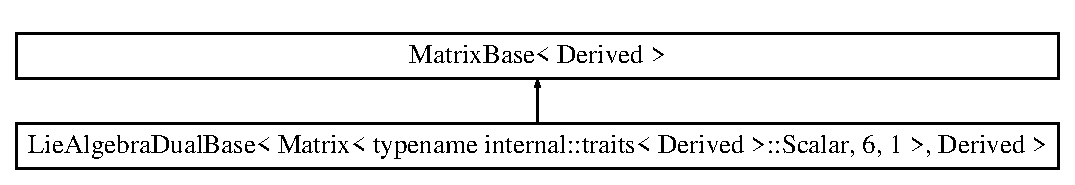
\includegraphics[height=2.000000cm]{class_lie_algebra_dual_base_3_01_matrix_3_01typename_01internal_1_1traits_3_01_derived_01_4_1_1_7557dc73cbfcbc32e399b9855a977d47}
\end{center}
\end{figure}
\subsection*{Public Types}
\begin{DoxyCompactItemize}
\item 
typedef Matrix$<$ Scalar, 6, 1 $>$ \hyperlink{class_lie_algebra_dual_base_3_01_matrix_3_01typename_01internal_1_1traits_3_01_derived_01_4_1_1_7557dc73cbfcbc32e399b9855a977d47_a9593517bd5d02d1330f7940eb5865eda}{Base\+Type}
\item 
typedef internal\+::traits$<$ Derived $>$\+::\hyperlink{class_lie_algebra_dual_base_3_01_matrix_3_01typename_01internal_1_1traits_3_01_derived_01_4_1_1_7557dc73cbfcbc32e399b9855a977d47_ac1756a8985eb67fcece03a1d4ac61111}{Coefficients} \hyperlink{class_lie_algebra_dual_base_3_01_matrix_3_01typename_01internal_1_1traits_3_01_derived_01_4_1_1_7557dc73cbfcbc32e399b9855a977d47_ac1756a8985eb67fcece03a1d4ac61111}{Coefficients}
\item 
typedef \hyperlink{class_lie_algebra_dual}{Lie\+Algebra\+Dual}$<$ \hyperlink{class_lie_algebra_dual_base_3_01_matrix_3_01typename_01internal_1_1traits_3_01_derived_01_4_1_1_7557dc73cbfcbc32e399b9855a977d47_a9593517bd5d02d1330f7940eb5865eda}{Base\+Type} $>$ \hyperlink{class_lie_algebra_dual_base_3_01_matrix_3_01typename_01internal_1_1traits_3_01_derived_01_4_1_1_7557dc73cbfcbc32e399b9855a977d47_a34fb3c6349c2f83f38780d146799886c}{Plain\+Object}
\item 
typedef \hyperlink{class_lie_algebra}{Lie\+Algebra}$<$ \hyperlink{class_lie_algebra_dual_base_3_01_matrix_3_01typename_01internal_1_1traits_3_01_derived_01_4_1_1_7557dc73cbfcbc32e399b9855a977d47_a9593517bd5d02d1330f7940eb5865eda}{Base\+Type} $>$ \hyperlink{class_lie_algebra_dual_base_3_01_matrix_3_01typename_01internal_1_1traits_3_01_derived_01_4_1_1_7557dc73cbfcbc32e399b9855a977d47_a834f0ffb501735f11a3328972a445078}{Algebra}
\item 
typedef Matrix$<$ Scalar, 3, 1 $>$ \hyperlink{class_lie_algebra_dual_base_3_01_matrix_3_01typename_01internal_1_1traits_3_01_derived_01_4_1_1_7557dc73cbfcbc32e399b9855a977d47_acd7fd5207d2c438f3f26f99eeedf280d}{Vector3}
\item 
typedef \hyperlink{class_lie_algebra_dual}{Lie\+Algebra\+Dual}$<$ Matrix$<$ Scalar, 3, 1 $>$ $>$ \hyperlink{class_lie_algebra_dual_base_3_01_matrix_3_01typename_01internal_1_1traits_3_01_derived_01_4_1_1_7557dc73cbfcbc32e399b9855a977d47_ab33be35099ff8bda572467ce899de5aa}{so3\+Element}
\end{DoxyCompactItemize}
\subsection*{Public Member Functions}
\begin{DoxyCompactItemize}
\item 
Map$<$ \hyperlink{class_lie_algebra_dual_base_3_01_matrix_3_01typename_01internal_1_1traits_3_01_derived_01_4_1_1_7557dc73cbfcbc32e399b9855a977d47_ab33be35099ff8bda572467ce899de5aa}{so3\+Element} $>$ \hyperlink{class_lie_algebra_dual_base_3_01_matrix_3_01typename_01internal_1_1traits_3_01_derived_01_4_1_1_7557dc73cbfcbc32e399b9855a977d47_a524db7791aae1703b62f8b30c974a287}{getso3\+Element} ()
\item 
Map$<$ const \hyperlink{class_lie_algebra_dual_base_3_01_matrix_3_01typename_01internal_1_1traits_3_01_derived_01_4_1_1_7557dc73cbfcbc32e399b9855a977d47_ab33be35099ff8bda572467ce899de5aa}{so3\+Element} $>$ \hyperlink{class_lie_algebra_dual_base_3_01_matrix_3_01typename_01internal_1_1traits_3_01_derived_01_4_1_1_7557dc73cbfcbc32e399b9855a977d47_a4c042c5fddf9a999e414d5f1b36a4221}{getso3\+Element} () const
\item 
Map$<$ \hyperlink{class_lie_algebra_dual_base_3_01_matrix_3_01typename_01internal_1_1traits_3_01_derived_01_4_1_1_7557dc73cbfcbc32e399b9855a977d47_acd7fd5207d2c438f3f26f99eeedf280d}{Vector3} $>$ \hyperlink{class_lie_algebra_dual_base_3_01_matrix_3_01typename_01internal_1_1traits_3_01_derived_01_4_1_1_7557dc73cbfcbc32e399b9855a977d47_abc22911715c749b5b21f5c65170ec3ea}{get\+R3\+Element} ()
\item 
Map$<$ const \hyperlink{class_lie_algebra_dual_base_3_01_matrix_3_01typename_01internal_1_1traits_3_01_derived_01_4_1_1_7557dc73cbfcbc32e399b9855a977d47_acd7fd5207d2c438f3f26f99eeedf280d}{Vector3} $>$ \hyperlink{class_lie_algebra_dual_base_3_01_matrix_3_01typename_01internal_1_1traits_3_01_derived_01_4_1_1_7557dc73cbfcbc32e399b9855a977d47_a796dd32c716dc56d80484b799f7031b5}{get\+R3\+Element} () const
\item 
\hyperlink{class_lie_algebra_dual_base_3_01_matrix_3_01typename_01internal_1_1traits_3_01_derived_01_4_1_1_7557dc73cbfcbc32e399b9855a977d47_ac1756a8985eb67fcece03a1d4ac61111}{Coefficients} \& \hyperlink{class_lie_algebra_dual_base_3_01_matrix_3_01typename_01internal_1_1traits_3_01_derived_01_4_1_1_7557dc73cbfcbc32e399b9855a977d47_ab589c3ff57eafff4e03df29ad2671565}{get} ()
\item 
const \hyperlink{class_lie_algebra_dual_base_3_01_matrix_3_01typename_01internal_1_1traits_3_01_derived_01_4_1_1_7557dc73cbfcbc32e399b9855a977d47_ac1756a8985eb67fcece03a1d4ac61111}{Coefficients} \& \hyperlink{class_lie_algebra_dual_base_3_01_matrix_3_01typename_01internal_1_1traits_3_01_derived_01_4_1_1_7557dc73cbfcbc32e399b9855a977d47_a476e5cee196fd72c7107203b50af1e69}{get} () const
\end{DoxyCompactItemize}
\subsection*{Protected Types}
\begin{DoxyCompactItemize}
\item 
typedef Matrix\+Base$<$ Derived $>$ \hyperlink{class_lie_algebra_dual_base_3_01_matrix_3_01typename_01internal_1_1traits_3_01_derived_01_4_1_1_7557dc73cbfcbc32e399b9855a977d47_a13f7decf31323f6148ba81f7431a8bac}{Base}
\end{DoxyCompactItemize}


\subsection{Detailed Description}
\subsubsection*{template$<$class Derived$>$\newline
class Lie\+Algebra\+Dual\+Base$<$ Matrix$<$ typename internal\+::traits$<$ Derived $>$\+::\+Scalar, 6, 1 $>$, Derived $>$}

Base class for the Lie algebra dual se$\ast$(3). 


\begin{DoxyTemplParams}{Template Parameters}
{\em Derived} & the derived class holding the coefficients which are of type Array$<$\+Scalar, 6, 1$>$ or Map$<$Array$<$\+Scalar, 6, 1$>$ $>$\\
\hline
\end{DoxyTemplParams}
This class actually implements methods form \hyperlink{class_lie_algebra_dual_base}{Lie\+Algebra\+Dual\+Base} for se$\ast$(3). Since se$\ast$(3) is the semi direct product of R$^\wedge$3 and so$\ast$(3) many operations are performed using directly elements form R$^\wedge$3 or so$\ast$(3)

a Lie algebra dual is also a vector Space (check if it\textquotesingle{}s true in the general case) that\textquotesingle{}s why it\textquotesingle{}s inherited from Matrix\+Base 

Definition at line 183 of file Lie\+Algebra\+\_\+se3.\+h.



\subsection{Member Typedef Documentation}
\hypertarget{class_lie_algebra_dual_base_3_01_matrix_3_01typename_01internal_1_1traits_3_01_derived_01_4_1_1_7557dc73cbfcbc32e399b9855a977d47_a834f0ffb501735f11a3328972a445078}{}\label{class_lie_algebra_dual_base_3_01_matrix_3_01typename_01internal_1_1traits_3_01_derived_01_4_1_1_7557dc73cbfcbc32e399b9855a977d47_a834f0ffb501735f11a3328972a445078} 
\index{Lie\+Algebra\+Dual\+Base$<$ Matrix$<$ typename internal\+::traits$<$ Derived $>$\+::\+Scalar, 6, 1 $>$, Derived $>$@{Lie\+Algebra\+Dual\+Base$<$ Matrix$<$ typename internal\+::traits$<$ Derived $>$\+::\+Scalar, 6, 1 $>$, Derived $>$}!Algebra@{Algebra}}
\index{Algebra@{Algebra}!Lie\+Algebra\+Dual\+Base$<$ Matrix$<$ typename internal\+::traits$<$ Derived $>$\+::\+Scalar, 6, 1 $>$, Derived $>$@{Lie\+Algebra\+Dual\+Base$<$ Matrix$<$ typename internal\+::traits$<$ Derived $>$\+::\+Scalar, 6, 1 $>$, Derived $>$}}
\subsubsection{\texorpdfstring{Algebra}{Algebra}}
{\footnotesize\ttfamily template$<$class Derived $>$ \\
typedef \hyperlink{class_lie_algebra}{Lie\+Algebra}$<$\hyperlink{class_lie_algebra_dual_base_3_01_matrix_3_01typename_01internal_1_1traits_3_01_derived_01_4_1_1_7557dc73cbfcbc32e399b9855a977d47_a9593517bd5d02d1330f7940eb5865eda}{Base\+Type}$>$ \hyperlink{class_lie_algebra_dual_base}{Lie\+Algebra\+Dual\+Base}$<$ Matrix$<$ typename internal\+::traits$<$ Derived $>$\+::Scalar, 6, 1 $>$, Derived $>$\+::\hyperlink{class_lie_algebra_dual_base_3_01_matrix_3_01typename_01internal_1_1traits_3_01_derived_01_4_1_1_7557dc73cbfcbc32e399b9855a977d47_a834f0ffb501735f11a3328972a445078}{Algebra}}

The type of the dual Algebra 

Definition at line 202 of file Lie\+Algebra\+\_\+se3.\+h.

\hypertarget{class_lie_algebra_dual_base_3_01_matrix_3_01typename_01internal_1_1traits_3_01_derived_01_4_1_1_7557dc73cbfcbc32e399b9855a977d47_a13f7decf31323f6148ba81f7431a8bac}{}\label{class_lie_algebra_dual_base_3_01_matrix_3_01typename_01internal_1_1traits_3_01_derived_01_4_1_1_7557dc73cbfcbc32e399b9855a977d47_a13f7decf31323f6148ba81f7431a8bac} 
\index{Lie\+Algebra\+Dual\+Base$<$ Matrix$<$ typename internal\+::traits$<$ Derived $>$\+::\+Scalar, 6, 1 $>$, Derived $>$@{Lie\+Algebra\+Dual\+Base$<$ Matrix$<$ typename internal\+::traits$<$ Derived $>$\+::\+Scalar, 6, 1 $>$, Derived $>$}!Base@{Base}}
\index{Base@{Base}!Lie\+Algebra\+Dual\+Base$<$ Matrix$<$ typename internal\+::traits$<$ Derived $>$\+::\+Scalar, 6, 1 $>$, Derived $>$@{Lie\+Algebra\+Dual\+Base$<$ Matrix$<$ typename internal\+::traits$<$ Derived $>$\+::\+Scalar, 6, 1 $>$, Derived $>$}}
\subsubsection{\texorpdfstring{Base}{Base}}
{\footnotesize\ttfamily template$<$class Derived $>$ \\
typedef Matrix\+Base$<$Derived$>$ \hyperlink{class_lie_algebra_dual_base}{Lie\+Algebra\+Dual\+Base}$<$ Matrix$<$ typename internal\+::traits$<$ Derived $>$\+::Scalar, 6, 1 $>$, Derived $>$\+::\hyperlink{class_lie_algebra_dual_base_3_01_matrix_3_01typename_01internal_1_1traits_3_01_derived_01_4_1_1_7557dc73cbfcbc32e399b9855a977d47_a13f7decf31323f6148ba81f7431a8bac}{Base}\hspace{0.3cm}{\ttfamily [protected]}}

The inherited class 

Definition at line 186 of file Lie\+Algebra\+\_\+se3.\+h.

\hypertarget{class_lie_algebra_dual_base_3_01_matrix_3_01typename_01internal_1_1traits_3_01_derived_01_4_1_1_7557dc73cbfcbc32e399b9855a977d47_a9593517bd5d02d1330f7940eb5865eda}{}\label{class_lie_algebra_dual_base_3_01_matrix_3_01typename_01internal_1_1traits_3_01_derived_01_4_1_1_7557dc73cbfcbc32e399b9855a977d47_a9593517bd5d02d1330f7940eb5865eda} 
\index{Lie\+Algebra\+Dual\+Base$<$ Matrix$<$ typename internal\+::traits$<$ Derived $>$\+::\+Scalar, 6, 1 $>$, Derived $>$@{Lie\+Algebra\+Dual\+Base$<$ Matrix$<$ typename internal\+::traits$<$ Derived $>$\+::\+Scalar, 6, 1 $>$, Derived $>$}!Base\+Type@{Base\+Type}}
\index{Base\+Type@{Base\+Type}!Lie\+Algebra\+Dual\+Base$<$ Matrix$<$ typename internal\+::traits$<$ Derived $>$\+::\+Scalar, 6, 1 $>$, Derived $>$@{Lie\+Algebra\+Dual\+Base$<$ Matrix$<$ typename internal\+::traits$<$ Derived $>$\+::\+Scalar, 6, 1 $>$, Derived $>$}}
\subsubsection{\texorpdfstring{Base\+Type}{BaseType}}
{\footnotesize\ttfamily template$<$class Derived $>$ \\
typedef Matrix$<$Scalar, 6, 1$>$ \hyperlink{class_lie_algebra_dual_base}{Lie\+Algebra\+Dual\+Base}$<$ Matrix$<$ typename internal\+::traits$<$ Derived $>$\+::Scalar, 6, 1 $>$, Derived $>$\+::\hyperlink{class_lie_algebra_dual_base_3_01_matrix_3_01typename_01internal_1_1traits_3_01_derived_01_4_1_1_7557dc73cbfcbc32e399b9855a977d47_a9593517bd5d02d1330f7940eb5865eda}{Base\+Type}}

The wrapped class 

Definition at line 196 of file Lie\+Algebra\+\_\+se3.\+h.

\hypertarget{class_lie_algebra_dual_base_3_01_matrix_3_01typename_01internal_1_1traits_3_01_derived_01_4_1_1_7557dc73cbfcbc32e399b9855a977d47_ac1756a8985eb67fcece03a1d4ac61111}{}\label{class_lie_algebra_dual_base_3_01_matrix_3_01typename_01internal_1_1traits_3_01_derived_01_4_1_1_7557dc73cbfcbc32e399b9855a977d47_ac1756a8985eb67fcece03a1d4ac61111} 
\index{Lie\+Algebra\+Dual\+Base$<$ Matrix$<$ typename internal\+::traits$<$ Derived $>$\+::\+Scalar, 6, 1 $>$, Derived $>$@{Lie\+Algebra\+Dual\+Base$<$ Matrix$<$ typename internal\+::traits$<$ Derived $>$\+::\+Scalar, 6, 1 $>$, Derived $>$}!Coefficients@{Coefficients}}
\index{Coefficients@{Coefficients}!Lie\+Algebra\+Dual\+Base$<$ Matrix$<$ typename internal\+::traits$<$ Derived $>$\+::\+Scalar, 6, 1 $>$, Derived $>$@{Lie\+Algebra\+Dual\+Base$<$ Matrix$<$ typename internal\+::traits$<$ Derived $>$\+::\+Scalar, 6, 1 $>$, Derived $>$}}
\subsubsection{\texorpdfstring{Coefficients}{Coefficients}}
{\footnotesize\ttfamily template$<$class Derived $>$ \\
typedef internal\+::traits$<$Derived$>$\+::\hyperlink{class_lie_algebra_dual_base_3_01_matrix_3_01typename_01internal_1_1traits_3_01_derived_01_4_1_1_7557dc73cbfcbc32e399b9855a977d47_ac1756a8985eb67fcece03a1d4ac61111}{Coefficients} \hyperlink{class_lie_algebra_dual_base}{Lie\+Algebra\+Dual\+Base}$<$ Matrix$<$ typename internal\+::traits$<$ Derived $>$\+::Scalar, 6, 1 $>$, Derived $>$\+::\hyperlink{class_lie_algebra_dual_base_3_01_matrix_3_01typename_01internal_1_1traits_3_01_derived_01_4_1_1_7557dc73cbfcbc32e399b9855a977d47_ac1756a8985eb67fcece03a1d4ac61111}{Coefficients}}

The kind of stored coefficients 

Definition at line 198 of file Lie\+Algebra\+\_\+se3.\+h.

\hypertarget{class_lie_algebra_dual_base_3_01_matrix_3_01typename_01internal_1_1traits_3_01_derived_01_4_1_1_7557dc73cbfcbc32e399b9855a977d47_a34fb3c6349c2f83f38780d146799886c}{}\label{class_lie_algebra_dual_base_3_01_matrix_3_01typename_01internal_1_1traits_3_01_derived_01_4_1_1_7557dc73cbfcbc32e399b9855a977d47_a34fb3c6349c2f83f38780d146799886c} 
\index{Lie\+Algebra\+Dual\+Base$<$ Matrix$<$ typename internal\+::traits$<$ Derived $>$\+::\+Scalar, 6, 1 $>$, Derived $>$@{Lie\+Algebra\+Dual\+Base$<$ Matrix$<$ typename internal\+::traits$<$ Derived $>$\+::\+Scalar, 6, 1 $>$, Derived $>$}!Plain\+Object@{Plain\+Object}}
\index{Plain\+Object@{Plain\+Object}!Lie\+Algebra\+Dual\+Base$<$ Matrix$<$ typename internal\+::traits$<$ Derived $>$\+::\+Scalar, 6, 1 $>$, Derived $>$@{Lie\+Algebra\+Dual\+Base$<$ Matrix$<$ typename internal\+::traits$<$ Derived $>$\+::\+Scalar, 6, 1 $>$, Derived $>$}}
\subsubsection{\texorpdfstring{Plain\+Object}{PlainObject}}
{\footnotesize\ttfamily template$<$class Derived $>$ \\
typedef \hyperlink{class_lie_algebra_dual}{Lie\+Algebra\+Dual}$<$\hyperlink{class_lie_algebra_dual_base_3_01_matrix_3_01typename_01internal_1_1traits_3_01_derived_01_4_1_1_7557dc73cbfcbc32e399b9855a977d47_a9593517bd5d02d1330f7940eb5865eda}{Base\+Type}$>$ \hyperlink{class_lie_algebra_dual_base}{Lie\+Algebra\+Dual\+Base}$<$ Matrix$<$ typename internal\+::traits$<$ Derived $>$\+::Scalar, 6, 1 $>$, Derived $>$\+::\hyperlink{class_lie_algebra_dual_base_3_01_matrix_3_01typename_01internal_1_1traits_3_01_derived_01_4_1_1_7557dc73cbfcbc32e399b9855a977d47_a34fb3c6349c2f83f38780d146799886c}{Plain\+Object}}

The plain object returned, while using Map$<$Lie\+Algebra$<$ $>$ $>$ 

Definition at line 200 of file Lie\+Algebra\+\_\+se3.\+h.

\hypertarget{class_lie_algebra_dual_base_3_01_matrix_3_01typename_01internal_1_1traits_3_01_derived_01_4_1_1_7557dc73cbfcbc32e399b9855a977d47_ab33be35099ff8bda572467ce899de5aa}{}\label{class_lie_algebra_dual_base_3_01_matrix_3_01typename_01internal_1_1traits_3_01_derived_01_4_1_1_7557dc73cbfcbc32e399b9855a977d47_ab33be35099ff8bda572467ce899de5aa} 
\index{Lie\+Algebra\+Dual\+Base$<$ Matrix$<$ typename internal\+::traits$<$ Derived $>$\+::\+Scalar, 6, 1 $>$, Derived $>$@{Lie\+Algebra\+Dual\+Base$<$ Matrix$<$ typename internal\+::traits$<$ Derived $>$\+::\+Scalar, 6, 1 $>$, Derived $>$}!so3\+Element@{so3\+Element}}
\index{so3\+Element@{so3\+Element}!Lie\+Algebra\+Dual\+Base$<$ Matrix$<$ typename internal\+::traits$<$ Derived $>$\+::\+Scalar, 6, 1 $>$, Derived $>$@{Lie\+Algebra\+Dual\+Base$<$ Matrix$<$ typename internal\+::traits$<$ Derived $>$\+::\+Scalar, 6, 1 $>$, Derived $>$}}
\subsubsection{\texorpdfstring{so3\+Element}{so3Element}}
{\footnotesize\ttfamily template$<$class Derived $>$ \\
typedef \hyperlink{class_lie_algebra_dual}{Lie\+Algebra\+Dual}$<$Matrix$<$Scalar, 3, 1$>$ $>$ \hyperlink{class_lie_algebra_dual_base}{Lie\+Algebra\+Dual\+Base}$<$ Matrix$<$ typename internal\+::traits$<$ Derived $>$\+::Scalar, 6, 1 $>$, Derived $>$\+::\hyperlink{class_lie_algebra_dual_base_3_01_matrix_3_01typename_01internal_1_1traits_3_01_derived_01_4_1_1_7557dc73cbfcbc32e399b9855a977d47_ab33be35099ff8bda572467ce899de5aa}{so3\+Element}}

The type of an element of so$\ast$(3) 

Definition at line 207 of file Lie\+Algebra\+\_\+se3.\+h.

\hypertarget{class_lie_algebra_dual_base_3_01_matrix_3_01typename_01internal_1_1traits_3_01_derived_01_4_1_1_7557dc73cbfcbc32e399b9855a977d47_acd7fd5207d2c438f3f26f99eeedf280d}{}\label{class_lie_algebra_dual_base_3_01_matrix_3_01typename_01internal_1_1traits_3_01_derived_01_4_1_1_7557dc73cbfcbc32e399b9855a977d47_acd7fd5207d2c438f3f26f99eeedf280d} 
\index{Lie\+Algebra\+Dual\+Base$<$ Matrix$<$ typename internal\+::traits$<$ Derived $>$\+::\+Scalar, 6, 1 $>$, Derived $>$@{Lie\+Algebra\+Dual\+Base$<$ Matrix$<$ typename internal\+::traits$<$ Derived $>$\+::\+Scalar, 6, 1 $>$, Derived $>$}!Vector3@{Vector3}}
\index{Vector3@{Vector3}!Lie\+Algebra\+Dual\+Base$<$ Matrix$<$ typename internal\+::traits$<$ Derived $>$\+::\+Scalar, 6, 1 $>$, Derived $>$@{Lie\+Algebra\+Dual\+Base$<$ Matrix$<$ typename internal\+::traits$<$ Derived $>$\+::\+Scalar, 6, 1 $>$, Derived $>$}}
\subsubsection{\texorpdfstring{Vector3}{Vector3}}
{\footnotesize\ttfamily template$<$class Derived $>$ \\
typedef Matrix$<$Scalar, 3, 1$>$ \hyperlink{class_lie_algebra_dual_base}{Lie\+Algebra\+Dual\+Base}$<$ Matrix$<$ typename internal\+::traits$<$ Derived $>$\+::Scalar, 6, 1 $>$, Derived $>$\+::\hyperlink{class_lie_algebra_dual_base_3_01_matrix_3_01typename_01internal_1_1traits_3_01_derived_01_4_1_1_7557dc73cbfcbc32e399b9855a977d47_acd7fd5207d2c438f3f26f99eeedf280d}{Vector3}}

The type of an element of R$^\wedge$3 

Definition at line 205 of file Lie\+Algebra\+\_\+se3.\+h.



\subsection{Member Function Documentation}
\hypertarget{class_lie_algebra_dual_base_3_01_matrix_3_01typename_01internal_1_1traits_3_01_derived_01_4_1_1_7557dc73cbfcbc32e399b9855a977d47_ab589c3ff57eafff4e03df29ad2671565}{}\label{class_lie_algebra_dual_base_3_01_matrix_3_01typename_01internal_1_1traits_3_01_derived_01_4_1_1_7557dc73cbfcbc32e399b9855a977d47_ab589c3ff57eafff4e03df29ad2671565} 
\index{Lie\+Algebra\+Dual\+Base$<$ Matrix$<$ typename internal\+::traits$<$ Derived $>$\+::\+Scalar, 6, 1 $>$, Derived $>$@{Lie\+Algebra\+Dual\+Base$<$ Matrix$<$ typename internal\+::traits$<$ Derived $>$\+::\+Scalar, 6, 1 $>$, Derived $>$}!get@{get}}
\index{get@{get}!Lie\+Algebra\+Dual\+Base$<$ Matrix$<$ typename internal\+::traits$<$ Derived $>$\+::\+Scalar, 6, 1 $>$, Derived $>$@{Lie\+Algebra\+Dual\+Base$<$ Matrix$<$ typename internal\+::traits$<$ Derived $>$\+::\+Scalar, 6, 1 $>$, Derived $>$}}
\subsubsection{\texorpdfstring{get()}{get()}\hspace{0.1cm}{\footnotesize\ttfamily [1/2]}}
{\footnotesize\ttfamily template$<$class Derived $>$ \\
\hyperlink{class_lie_algebra_dual_base_3_01_matrix_3_01typename_01internal_1_1traits_3_01_derived_01_4_1_1_7557dc73cbfcbc32e399b9855a977d47_ac1756a8985eb67fcece03a1d4ac61111}{Coefficients}\& \hyperlink{class_lie_algebra_dual_base}{Lie\+Algebra\+Dual\+Base}$<$ Matrix$<$ typename internal\+::traits$<$ Derived $>$\+::Scalar, 6, 1 $>$, Derived $>$\+::get (\begin{DoxyParamCaption}{ }\end{DoxyParamCaption})\hspace{0.3cm}{\ttfamily [inline]}}

\begin{DoxyReturn}{Returns}
The stored coefficients by the derived class 
\end{DoxyReturn}


Definition at line 219 of file Lie\+Algebra\+\_\+se3.\+h.

\hypertarget{class_lie_algebra_dual_base_3_01_matrix_3_01typename_01internal_1_1traits_3_01_derived_01_4_1_1_7557dc73cbfcbc32e399b9855a977d47_a476e5cee196fd72c7107203b50af1e69}{}\label{class_lie_algebra_dual_base_3_01_matrix_3_01typename_01internal_1_1traits_3_01_derived_01_4_1_1_7557dc73cbfcbc32e399b9855a977d47_a476e5cee196fd72c7107203b50af1e69} 
\index{Lie\+Algebra\+Dual\+Base$<$ Matrix$<$ typename internal\+::traits$<$ Derived $>$\+::\+Scalar, 6, 1 $>$, Derived $>$@{Lie\+Algebra\+Dual\+Base$<$ Matrix$<$ typename internal\+::traits$<$ Derived $>$\+::\+Scalar, 6, 1 $>$, Derived $>$}!get@{get}}
\index{get@{get}!Lie\+Algebra\+Dual\+Base$<$ Matrix$<$ typename internal\+::traits$<$ Derived $>$\+::\+Scalar, 6, 1 $>$, Derived $>$@{Lie\+Algebra\+Dual\+Base$<$ Matrix$<$ typename internal\+::traits$<$ Derived $>$\+::\+Scalar, 6, 1 $>$, Derived $>$}}
\subsubsection{\texorpdfstring{get()}{get()}\hspace{0.1cm}{\footnotesize\ttfamily [2/2]}}
{\footnotesize\ttfamily template$<$class Derived $>$ \\
const \hyperlink{class_lie_algebra_dual_base_3_01_matrix_3_01typename_01internal_1_1traits_3_01_derived_01_4_1_1_7557dc73cbfcbc32e399b9855a977d47_ac1756a8985eb67fcece03a1d4ac61111}{Coefficients}\& \hyperlink{class_lie_algebra_dual_base}{Lie\+Algebra\+Dual\+Base}$<$ Matrix$<$ typename internal\+::traits$<$ Derived $>$\+::Scalar, 6, 1 $>$, Derived $>$\+::get (\begin{DoxyParamCaption}{ }\end{DoxyParamCaption}) const\hspace{0.3cm}{\ttfamily [inline]}}

\begin{DoxyReturn}{Returns}
The read-\/only access to the stored coefficients by the derived class 
\end{DoxyReturn}


Definition at line 221 of file Lie\+Algebra\+\_\+se3.\+h.

\hypertarget{class_lie_algebra_dual_base_3_01_matrix_3_01typename_01internal_1_1traits_3_01_derived_01_4_1_1_7557dc73cbfcbc32e399b9855a977d47_abc22911715c749b5b21f5c65170ec3ea}{}\label{class_lie_algebra_dual_base_3_01_matrix_3_01typename_01internal_1_1traits_3_01_derived_01_4_1_1_7557dc73cbfcbc32e399b9855a977d47_abc22911715c749b5b21f5c65170ec3ea} 
\index{Lie\+Algebra\+Dual\+Base$<$ Matrix$<$ typename internal\+::traits$<$ Derived $>$\+::\+Scalar, 6, 1 $>$, Derived $>$@{Lie\+Algebra\+Dual\+Base$<$ Matrix$<$ typename internal\+::traits$<$ Derived $>$\+::\+Scalar, 6, 1 $>$, Derived $>$}!get\+R3\+Element@{get\+R3\+Element}}
\index{get\+R3\+Element@{get\+R3\+Element}!Lie\+Algebra\+Dual\+Base$<$ Matrix$<$ typename internal\+::traits$<$ Derived $>$\+::\+Scalar, 6, 1 $>$, Derived $>$@{Lie\+Algebra\+Dual\+Base$<$ Matrix$<$ typename internal\+::traits$<$ Derived $>$\+::\+Scalar, 6, 1 $>$, Derived $>$}}
\subsubsection{\texorpdfstring{get\+R3\+Element()}{getR3Element()}\hspace{0.1cm}{\footnotesize\ttfamily [1/2]}}
{\footnotesize\ttfamily template$<$class Derived $>$ \\
Map$<$\hyperlink{class_lie_algebra_dual_base_3_01_matrix_3_01typename_01internal_1_1traits_3_01_derived_01_4_1_1_7557dc73cbfcbc32e399b9855a977d47_acd7fd5207d2c438f3f26f99eeedf280d}{Vector3}$>$ \hyperlink{class_lie_algebra_dual_base}{Lie\+Algebra\+Dual\+Base}$<$ Matrix$<$ typename internal\+::traits$<$ Derived $>$\+::Scalar, 6, 1 $>$, Derived $>$\+::get\+R3\+Element (\begin{DoxyParamCaption}{ }\end{DoxyParamCaption})\hspace{0.3cm}{\ttfamily [inline]}}

The accessor to the R$^\wedge$3 element 

Definition at line 214 of file Lie\+Algebra\+\_\+se3.\+h.

\hypertarget{class_lie_algebra_dual_base_3_01_matrix_3_01typename_01internal_1_1traits_3_01_derived_01_4_1_1_7557dc73cbfcbc32e399b9855a977d47_a796dd32c716dc56d80484b799f7031b5}{}\label{class_lie_algebra_dual_base_3_01_matrix_3_01typename_01internal_1_1traits_3_01_derived_01_4_1_1_7557dc73cbfcbc32e399b9855a977d47_a796dd32c716dc56d80484b799f7031b5} 
\index{Lie\+Algebra\+Dual\+Base$<$ Matrix$<$ typename internal\+::traits$<$ Derived $>$\+::\+Scalar, 6, 1 $>$, Derived $>$@{Lie\+Algebra\+Dual\+Base$<$ Matrix$<$ typename internal\+::traits$<$ Derived $>$\+::\+Scalar, 6, 1 $>$, Derived $>$}!get\+R3\+Element@{get\+R3\+Element}}
\index{get\+R3\+Element@{get\+R3\+Element}!Lie\+Algebra\+Dual\+Base$<$ Matrix$<$ typename internal\+::traits$<$ Derived $>$\+::\+Scalar, 6, 1 $>$, Derived $>$@{Lie\+Algebra\+Dual\+Base$<$ Matrix$<$ typename internal\+::traits$<$ Derived $>$\+::\+Scalar, 6, 1 $>$, Derived $>$}}
\subsubsection{\texorpdfstring{get\+R3\+Element()}{getR3Element()}\hspace{0.1cm}{\footnotesize\ttfamily [2/2]}}
{\footnotesize\ttfamily template$<$class Derived $>$ \\
Map$<$const \hyperlink{class_lie_algebra_dual_base_3_01_matrix_3_01typename_01internal_1_1traits_3_01_derived_01_4_1_1_7557dc73cbfcbc32e399b9855a977d47_acd7fd5207d2c438f3f26f99eeedf280d}{Vector3}$>$ \hyperlink{class_lie_algebra_dual_base}{Lie\+Algebra\+Dual\+Base}$<$ Matrix$<$ typename internal\+::traits$<$ Derived $>$\+::Scalar, 6, 1 $>$, Derived $>$\+::get\+R3\+Element (\begin{DoxyParamCaption}{ }\end{DoxyParamCaption}) const\hspace{0.3cm}{\ttfamily [inline]}}

The read-\/only accessor to the R$^\wedge$3 element 

Definition at line 216 of file Lie\+Algebra\+\_\+se3.\+h.

\hypertarget{class_lie_algebra_dual_base_3_01_matrix_3_01typename_01internal_1_1traits_3_01_derived_01_4_1_1_7557dc73cbfcbc32e399b9855a977d47_a524db7791aae1703b62f8b30c974a287}{}\label{class_lie_algebra_dual_base_3_01_matrix_3_01typename_01internal_1_1traits_3_01_derived_01_4_1_1_7557dc73cbfcbc32e399b9855a977d47_a524db7791aae1703b62f8b30c974a287} 
\index{Lie\+Algebra\+Dual\+Base$<$ Matrix$<$ typename internal\+::traits$<$ Derived $>$\+::\+Scalar, 6, 1 $>$, Derived $>$@{Lie\+Algebra\+Dual\+Base$<$ Matrix$<$ typename internal\+::traits$<$ Derived $>$\+::\+Scalar, 6, 1 $>$, Derived $>$}!getso3\+Element@{getso3\+Element}}
\index{getso3\+Element@{getso3\+Element}!Lie\+Algebra\+Dual\+Base$<$ Matrix$<$ typename internal\+::traits$<$ Derived $>$\+::\+Scalar, 6, 1 $>$, Derived $>$@{Lie\+Algebra\+Dual\+Base$<$ Matrix$<$ typename internal\+::traits$<$ Derived $>$\+::\+Scalar, 6, 1 $>$, Derived $>$}}
\subsubsection{\texorpdfstring{getso3\+Element()}{getso3Element()}\hspace{0.1cm}{\footnotesize\ttfamily [1/2]}}
{\footnotesize\ttfamily template$<$class Derived $>$ \\
Map$<$\hyperlink{class_lie_algebra_dual_base_3_01_matrix_3_01typename_01internal_1_1traits_3_01_derived_01_4_1_1_7557dc73cbfcbc32e399b9855a977d47_ab33be35099ff8bda572467ce899de5aa}{so3\+Element}$>$ \hyperlink{class_lie_algebra_dual_base}{Lie\+Algebra\+Dual\+Base}$<$ Matrix$<$ typename internal\+::traits$<$ Derived $>$\+::Scalar, 6, 1 $>$, Derived $>$\+::getso3\+Element (\begin{DoxyParamCaption}{ }\end{DoxyParamCaption})\hspace{0.3cm}{\ttfamily [inline]}}

The accessor to the so(3) element 

Definition at line 210 of file Lie\+Algebra\+\_\+se3.\+h.

\hypertarget{class_lie_algebra_dual_base_3_01_matrix_3_01typename_01internal_1_1traits_3_01_derived_01_4_1_1_7557dc73cbfcbc32e399b9855a977d47_a4c042c5fddf9a999e414d5f1b36a4221}{}\label{class_lie_algebra_dual_base_3_01_matrix_3_01typename_01internal_1_1traits_3_01_derived_01_4_1_1_7557dc73cbfcbc32e399b9855a977d47_a4c042c5fddf9a999e414d5f1b36a4221} 
\index{Lie\+Algebra\+Dual\+Base$<$ Matrix$<$ typename internal\+::traits$<$ Derived $>$\+::\+Scalar, 6, 1 $>$, Derived $>$@{Lie\+Algebra\+Dual\+Base$<$ Matrix$<$ typename internal\+::traits$<$ Derived $>$\+::\+Scalar, 6, 1 $>$, Derived $>$}!getso3\+Element@{getso3\+Element}}
\index{getso3\+Element@{getso3\+Element}!Lie\+Algebra\+Dual\+Base$<$ Matrix$<$ typename internal\+::traits$<$ Derived $>$\+::\+Scalar, 6, 1 $>$, Derived $>$@{Lie\+Algebra\+Dual\+Base$<$ Matrix$<$ typename internal\+::traits$<$ Derived $>$\+::\+Scalar, 6, 1 $>$, Derived $>$}}
\subsubsection{\texorpdfstring{getso3\+Element()}{getso3Element()}\hspace{0.1cm}{\footnotesize\ttfamily [2/2]}}
{\footnotesize\ttfamily template$<$class Derived $>$ \\
Map$<$const \hyperlink{class_lie_algebra_dual_base_3_01_matrix_3_01typename_01internal_1_1traits_3_01_derived_01_4_1_1_7557dc73cbfcbc32e399b9855a977d47_ab33be35099ff8bda572467ce899de5aa}{so3\+Element}$>$ \hyperlink{class_lie_algebra_dual_base}{Lie\+Algebra\+Dual\+Base}$<$ Matrix$<$ typename internal\+::traits$<$ Derived $>$\+::Scalar, 6, 1 $>$, Derived $>$\+::getso3\+Element (\begin{DoxyParamCaption}{ }\end{DoxyParamCaption}) const\hspace{0.3cm}{\ttfamily [inline]}}

The read-\/only accessor to the so(3) element 

Definition at line 212 of file Lie\+Algebra\+\_\+se3.\+h.



The documentation for this class was generated from the following file\+:\begin{DoxyCompactItemize}
\item 
/\+Users/\+Ryan/\+Code/codyco-\/superbuild/libraries/\+Eigen\+Lgsm/unsupported/\+Eigen/src/\+Lgsm/\hyperlink{_lie_algebra__se3_8h}{Lie\+Algebra\+\_\+se3.\+h}\end{DoxyCompactItemize}

\hypertarget{class_lie_group}{}\section{Lie\+Group$<$ G $>$ Class Template Reference}
\label{class_lie_group}\index{Lie\+Group$<$ G $>$@{Lie\+Group$<$ G $>$}}


Class describing an element of a Lie Group.  




{\ttfamily \#include $<$Lie\+Group.\+h$>$}

Inheritance diagram for Lie\+Group$<$ G $>$\+:\begin{figure}[H]
\begin{center}
\leavevmode
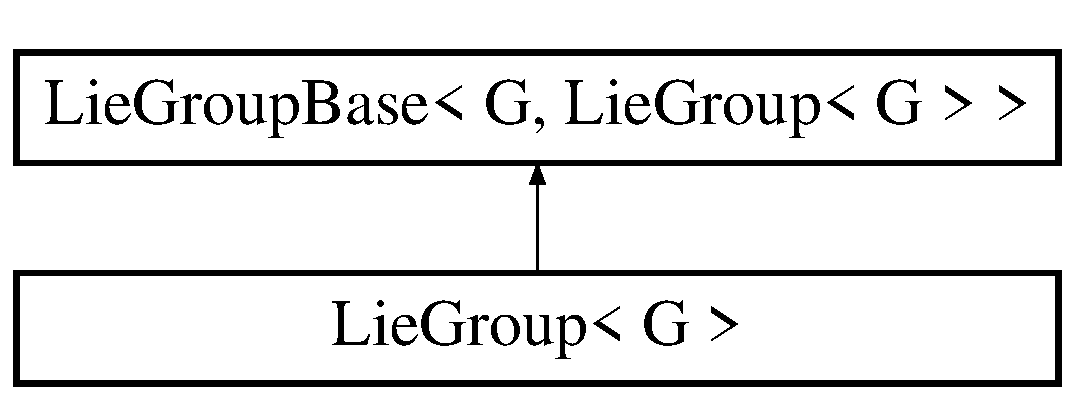
\includegraphics[height=2.000000cm]{class_lie_group}
\end{center}
\end{figure}
\subsection*{Public Types}
\begin{DoxyCompactItemize}
\item 
typedef internal\+::traits$<$ \hyperlink{class_lie_group}{Lie\+Group}$<$ G $>$ $>$\+::\hyperlink{class_lie_group_a52de3c5adb933cbfa694b51bef656d5d}{Coefficients} \hyperlink{class_lie_group_a52de3c5adb933cbfa694b51bef656d5d}{Coefficients}
\end{DoxyCompactItemize}
\subsection*{Public Member Functions}
\begin{DoxyCompactItemize}
\item 
\hyperlink{class_lie_group_a9c6f35315929138296ec52903f347bff}{Lie\+Group} (const \hyperlink{class_lie_group}{Lie\+Group} \&)
\item 
\hyperlink{class_lie_group_ac831365f2877426d28524f26ab771525}{Lie\+Group} ()
\item 
\hyperlink{class_lie_group_a52de3c5adb933cbfa694b51bef656d5d}{Coefficients} \& \hyperlink{class_lie_group_ac8a00eee2b7425186ddf51dbf2e62f14}{get} ()
\item 
const \hyperlink{class_lie_group_a52de3c5adb933cbfa694b51bef656d5d}{Coefficients} \& \hyperlink{class_lie_group_aa551249eab20e2ba4778fc4753e09fd0}{get} () const
\end{DoxyCompactItemize}
\subsection*{Protected Types}
\begin{DoxyCompactItemize}
\item 
typedef \hyperlink{class_lie_group_base}{Lie\+Group\+Base}$<$ G, \hyperlink{class_lie_group}{Lie\+Group}$<$ G $>$ $>$ \hyperlink{class_lie_group_aac708f8905d0a77bbe8c9bae8c6ac525}{Base}
\end{DoxyCompactItemize}
\subsection*{Protected Attributes}
\begin{DoxyCompactItemize}
\item 
\hyperlink{class_lie_group_a52de3c5adb933cbfa694b51bef656d5d}{Coefficients} \hyperlink{class_lie_group_a8a312c03fa7d4fed55b4c26d4fe3057a}{m\+\_\+coeffs}
\end{DoxyCompactItemize}
\subsection*{Additional Inherited Members}


\subsection{Detailed Description}
\subsubsection*{template$<$class G$>$\newline
class Lie\+Group$<$ G $>$}

Class describing an element of a Lie Group. 

Definition of Lie\+Group$<$\+G$>$


\begin{DoxyTemplParams}{Template Parameters}
{\em G} & the wrapped class\\
\hline
\end{DoxyTemplParams}
This class must be specialized to add new constructors for a specific group.

\begin{DoxySeeAlso}{See also}
The methods are defined in \hyperlink{class_lie_group_base}{Lie\+Group\+Base} 
\end{DoxySeeAlso}


Definition at line 117 of file Lie\+Group.\+h.



\subsection{Member Typedef Documentation}
\hypertarget{class_lie_group_aac708f8905d0a77bbe8c9bae8c6ac525}{}\label{class_lie_group_aac708f8905d0a77bbe8c9bae8c6ac525} 
\index{Lie\+Group@{Lie\+Group}!Base@{Base}}
\index{Base@{Base}!Lie\+Group@{Lie\+Group}}
\subsubsection{\texorpdfstring{Base}{Base}}
{\footnotesize\ttfamily template$<$class G $>$ \\
typedef \hyperlink{class_lie_group_base}{Lie\+Group\+Base}$<$G, \hyperlink{class_lie_group}{Lie\+Group}$<$G$>$ $>$ \hyperlink{class_lie_group}{Lie\+Group}$<$ G $>$\+::\hyperlink{class_lie_group_aac708f8905d0a77bbe8c9bae8c6ac525}{Base}\hspace{0.3cm}{\ttfamily [protected]}}

Inherited class 

Definition at line 120 of file Lie\+Group.\+h.

\hypertarget{class_lie_group_a52de3c5adb933cbfa694b51bef656d5d}{}\label{class_lie_group_a52de3c5adb933cbfa694b51bef656d5d} 
\index{Lie\+Group@{Lie\+Group}!Coefficients@{Coefficients}}
\index{Coefficients@{Coefficients}!Lie\+Group@{Lie\+Group}}
\subsubsection{\texorpdfstring{Coefficients}{Coefficients}}
{\footnotesize\ttfamily template$<$class G $>$ \\
typedef internal\+::traits$<$\hyperlink{class_lie_group}{Lie\+Group}$<$G$>$ $>$\+::\hyperlink{class_lie_group_a52de3c5adb933cbfa694b51bef656d5d}{Coefficients} \hyperlink{class_lie_group}{Lie\+Group}$<$ G $>$\+::\hyperlink{class_lie_group_a52de3c5adb933cbfa694b51bef656d5d}{Coefficients}}

The stored coefficients 

Definition at line 126 of file Lie\+Group.\+h.



\subsection{Constructor \& Destructor Documentation}
\hypertarget{class_lie_group_a9c6f35315929138296ec52903f347bff}{}\label{class_lie_group_a9c6f35315929138296ec52903f347bff} 
\index{Lie\+Group@{Lie\+Group}!Lie\+Group@{Lie\+Group}}
\index{Lie\+Group@{Lie\+Group}!Lie\+Group@{Lie\+Group}}
\subsubsection{\texorpdfstring{Lie\+Group()}{LieGroup()}\hspace{0.1cm}{\footnotesize\ttfamily [1/2]}}
{\footnotesize\ttfamily template$<$class G $>$ \\
\hyperlink{class_lie_group}{Lie\+Group}$<$ G $>$\+::\hyperlink{class_lie_group}{Lie\+Group} (\begin{DoxyParamCaption}\item[{const \hyperlink{class_lie_group}{Lie\+Group}$<$ G $>$ \&}]{ }\end{DoxyParamCaption})\hspace{0.3cm}{\ttfamily [inline]}}

Copy constructor \+: do nothing 

Definition at line 129 of file Lie\+Group.\+h.

\hypertarget{class_lie_group_ac831365f2877426d28524f26ab771525}{}\label{class_lie_group_ac831365f2877426d28524f26ab771525} 
\index{Lie\+Group@{Lie\+Group}!Lie\+Group@{Lie\+Group}}
\index{Lie\+Group@{Lie\+Group}!Lie\+Group@{Lie\+Group}}
\subsubsection{\texorpdfstring{Lie\+Group()}{LieGroup()}\hspace{0.1cm}{\footnotesize\ttfamily [2/2]}}
{\footnotesize\ttfamily template$<$class G $>$ \\
\hyperlink{class_lie_group}{Lie\+Group}$<$ G $>$\+::\hyperlink{class_lie_group}{Lie\+Group} (\begin{DoxyParamCaption}{ }\end{DoxyParamCaption})\hspace{0.3cm}{\ttfamily [inline]}}

Constructor \+: do nothing 

Definition at line 131 of file Lie\+Group.\+h.



\subsection{Member Function Documentation}
\hypertarget{class_lie_group_ac8a00eee2b7425186ddf51dbf2e62f14}{}\label{class_lie_group_ac8a00eee2b7425186ddf51dbf2e62f14} 
\index{Lie\+Group@{Lie\+Group}!get@{get}}
\index{get@{get}!Lie\+Group@{Lie\+Group}}
\subsubsection{\texorpdfstring{get()}{get()}\hspace{0.1cm}{\footnotesize\ttfamily [1/2]}}
{\footnotesize\ttfamily template$<$class G $>$ \\
\hyperlink{class_lie_group_a52de3c5adb933cbfa694b51bef656d5d}{Coefficients}\& \hyperlink{class_lie_group}{Lie\+Group}$<$ G $>$\+::get (\begin{DoxyParamCaption}{ }\end{DoxyParamCaption})\hspace{0.3cm}{\ttfamily [inline]}}

\begin{DoxyReturn}{Returns}
The stored coefficients 
\end{DoxyReturn}


Definition at line 134 of file Lie\+Group.\+h.

\hypertarget{class_lie_group_aa551249eab20e2ba4778fc4753e09fd0}{}\label{class_lie_group_aa551249eab20e2ba4778fc4753e09fd0} 
\index{Lie\+Group@{Lie\+Group}!get@{get}}
\index{get@{get}!Lie\+Group@{Lie\+Group}}
\subsubsection{\texorpdfstring{get()}{get()}\hspace{0.1cm}{\footnotesize\ttfamily [2/2]}}
{\footnotesize\ttfamily template$<$class G $>$ \\
const \hyperlink{class_lie_group_a52de3c5adb933cbfa694b51bef656d5d}{Coefficients}\& \hyperlink{class_lie_group}{Lie\+Group}$<$ G $>$\+::get (\begin{DoxyParamCaption}{ }\end{DoxyParamCaption}) const\hspace{0.3cm}{\ttfamily [inline]}}

\begin{DoxyReturn}{Returns}
The read-\/only access to the stored coefficients 
\end{DoxyReturn}


Definition at line 136 of file Lie\+Group.\+h.



\subsection{Member Data Documentation}
\hypertarget{class_lie_group_a8a312c03fa7d4fed55b4c26d4fe3057a}{}\label{class_lie_group_a8a312c03fa7d4fed55b4c26d4fe3057a} 
\index{Lie\+Group@{Lie\+Group}!m\+\_\+coeffs@{m\+\_\+coeffs}}
\index{m\+\_\+coeffs@{m\+\_\+coeffs}!Lie\+Group@{Lie\+Group}}
\subsubsection{\texorpdfstring{m\+\_\+coeffs}{m\_coeffs}}
{\footnotesize\ttfamily template$<$class G $>$ \\
\hyperlink{class_lie_group_a52de3c5adb933cbfa694b51bef656d5d}{Coefficients} \hyperlink{class_lie_group}{Lie\+Group}$<$ G $>$\+::m\+\_\+coeffs\hspace{0.3cm}{\ttfamily [protected]}}

The wrapped coefficients 

Definition at line 140 of file Lie\+Group.\+h.



The documentation for this class was generated from the following file\+:\begin{DoxyCompactItemize}
\item 
/\+Users/\+Ryan/\+Code/codyco-\/superbuild/libraries/\+Eigen\+Lgsm/unsupported/\+Eigen/src/\+Lgsm/\hyperlink{_lie_group_8h}{Lie\+Group.\+h}\end{DoxyCompactItemize}

\hypertarget{class_lie_group_3_01_array_3_01___scalar_00_017_00_011_01_4_01_4}{}\section{Lie\+Group$<$ Array$<$ \+\_\+\+Scalar, 7, 1 $>$ $>$ Class Template Reference}
\label{class_lie_group_3_01_array_3_01___scalar_00_017_00_011_01_4_01_4}\index{Lie\+Group$<$ Array$<$ \+\_\+\+Scalar, 7, 1 $>$ $>$@{Lie\+Group$<$ Array$<$ \+\_\+\+Scalar, 7, 1 $>$ $>$}}


Class for S\+E(3) Lie Group.  




{\ttfamily \#include $<$Lie\+Group\+\_\+\+S\+E3.\+h$>$}

Inheritance diagram for Lie\+Group$<$ Array$<$ \+\_\+\+Scalar, 7, 1 $>$ $>$\+:\begin{figure}[H]
\begin{center}
\leavevmode
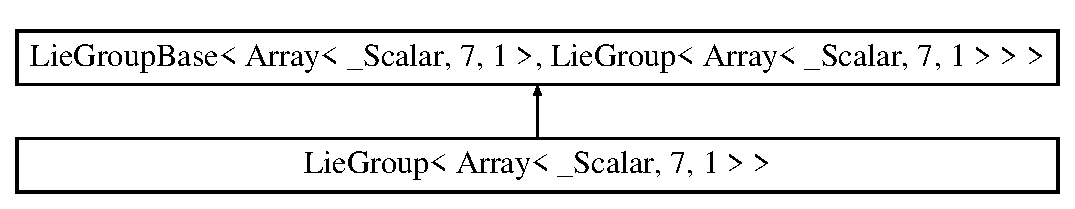
\includegraphics[height=2.000000cm]{class_lie_group_3_01_array_3_01___scalar_00_017_00_011_01_4_01_4}
\end{center}
\end{figure}
\subsection*{Public Types}
\begin{DoxyCompactItemize}
\item 
typedef \+\_\+\+Scalar \hyperlink{class_lie_group_3_01_array_3_01___scalar_00_017_00_011_01_4_01_4_a5fd29a7be3621d5df2717d910d47b3ce}{Scalar}
\item 
typedef internal\+::traits$<$ \hyperlink{class_lie_group}{Lie\+Group}$<$ Array$<$ \+\_\+\+Scalar, 7, 1 $>$ $>$ $>$\+::\hyperlink{class_lie_group_3_01_array_3_01___scalar_00_017_00_011_01_4_01_4_aa5d0fac468a8bdbb468bf2218b93ee0e}{Coefficients} \hyperlink{class_lie_group_3_01_array_3_01___scalar_00_017_00_011_01_4_01_4_aa5d0fac468a8bdbb468bf2218b93ee0e}{Coefficients}
\end{DoxyCompactItemize}
\subsection*{Public Member Functions}
\begin{DoxyCompactItemize}
\item 
\hyperlink{class_lie_group_3_01_array_3_01___scalar_00_017_00_011_01_4_01_4_a5f6d9e49b663a718f984052f5925a084}{Lie\+Group} ()
\item 
\hyperlink{class_lie_group_3_01_array_3_01___scalar_00_017_00_011_01_4_01_4_a87d24de69e4c7cd0eb139e57b7833f10}{Lie\+Group} (const \hyperlink{class_lie_group}{Lie\+Group} \&g)
\item 
\hyperlink{class_lie_group_3_01_array_3_01___scalar_00_017_00_011_01_4_01_4_a585f2bf44ee6cfefb3fcd80a40abe75d}{Lie\+Group} (const Array$<$ \hyperlink{class_lie_group_3_01_array_3_01___scalar_00_017_00_011_01_4_01_4_a5fd29a7be3621d5df2717d910d47b3ce}{Scalar}, 7, 1 $>$ \&g)
\item 
\hyperlink{class_lie_group_3_01_array_3_01___scalar_00_017_00_011_01_4_01_4_aa26a8dec73f9a261d811ae4f31b7647f}{Lie\+Group} (\hyperlink{class_lie_group_3_01_array_3_01___scalar_00_017_00_011_01_4_01_4_a5fd29a7be3621d5df2717d910d47b3ce}{Scalar} x, \hyperlink{class_lie_group_3_01_array_3_01___scalar_00_017_00_011_01_4_01_4_a5fd29a7be3621d5df2717d910d47b3ce}{Scalar} y, \hyperlink{class_lie_group_3_01_array_3_01___scalar_00_017_00_011_01_4_01_4_a5fd29a7be3621d5df2717d910d47b3ce}{Scalar} z, \hyperlink{class_lie_group_3_01_array_3_01___scalar_00_017_00_011_01_4_01_4_a5fd29a7be3621d5df2717d910d47b3ce}{Scalar} qw, \hyperlink{class_lie_group_3_01_array_3_01___scalar_00_017_00_011_01_4_01_4_a5fd29a7be3621d5df2717d910d47b3ce}{Scalar} qx, \hyperlink{class_lie_group_3_01_array_3_01___scalar_00_017_00_011_01_4_01_4_a5fd29a7be3621d5df2717d910d47b3ce}{Scalar} qy, \hyperlink{class_lie_group_3_01_array_3_01___scalar_00_017_00_011_01_4_01_4_a5fd29a7be3621d5df2717d910d47b3ce}{Scalar} qz)
\item 
E\+I\+G\+E\+N\+\_\+\+S\+T\+R\+O\+N\+G\+\_\+\+I\+N\+L\+I\+NE \hyperlink{class_lie_group_3_01_array_3_01___scalar_00_017_00_011_01_4_01_4_aca6a6a912e91782e43634a03f3eeb1ac}{Lie\+Group} (const typename Base\+::\+Vector3 \&v, const typename Base\+::\+S\+O3\+Element \&r)
\item 
{\footnotesize template$<$typename Derived $>$ }\\\hyperlink{class_lie_group_3_01_array_3_01___scalar_00_017_00_011_01_4_01_4_a97bbc79b1dfc73b9fd35f79c0bcfc3c4}{Lie\+Group} (const Matrix\+Base$<$ Derived $>$ \&other)
\item 
\hyperlink{class_lie_group_3_01_array_3_01___scalar_00_017_00_011_01_4_01_4_aa5d0fac468a8bdbb468bf2218b93ee0e}{Coefficients} \& \hyperlink{class_lie_group_3_01_array_3_01___scalar_00_017_00_011_01_4_01_4_ac1572d622034e7582584d2f01aa76e8e}{get} ()
\item 
const \hyperlink{class_lie_group_3_01_array_3_01___scalar_00_017_00_011_01_4_01_4_aa5d0fac468a8bdbb468bf2218b93ee0e}{Coefficients} \& \hyperlink{class_lie_group_3_01_array_3_01___scalar_00_017_00_011_01_4_01_4_a55244313e03e1da27920e4d7a17c2cd3}{get} () const
\end{DoxyCompactItemize}
\subsection*{Protected Types}
\begin{DoxyCompactItemize}
\item 
typedef \hyperlink{class_lie_group_base}{Lie\+Group\+Base}$<$ Array$<$ \+\_\+\+Scalar, 7, 1 $>$, \hyperlink{class_lie_group}{Lie\+Group}$<$ Array$<$ \+\_\+\+Scalar, 7, 1 $>$ $>$ $>$ \hyperlink{class_lie_group_3_01_array_3_01___scalar_00_017_00_011_01_4_01_4_a2f9c6357e55ba5e895a849c32e18b3c4}{Base}
\end{DoxyCompactItemize}
\subsection*{Protected Attributes}
\begin{DoxyCompactItemize}
\item 
\hyperlink{class_lie_group_3_01_array_3_01___scalar_00_017_00_011_01_4_01_4_aa5d0fac468a8bdbb468bf2218b93ee0e}{Coefficients} \hyperlink{class_lie_group_3_01_array_3_01___scalar_00_017_00_011_01_4_01_4_addbc1e13772e419af9c3cbea4d31bfdf}{m\+\_\+coeffs}
\end{DoxyCompactItemize}
\subsection*{Additional Inherited Members}


\subsection{Detailed Description}
\subsubsection*{template$<$typename \+\_\+\+Scalar$>$\newline
class Lie\+Group$<$ Array$<$ \+\_\+\+Scalar, 7, 1 $>$ $>$}

Class for S\+E(3) Lie Group. 

Definition of \hyperlink{class_lie_group}{Lie\+Group}$<$Array$<$\+Scalar, 7, 1$>$$>$


\begin{DoxyTemplParams}{Template Parameters}
{\em \+\_\+\+Scalar} & the type of the underlying array\\
\hline
\end{DoxyTemplParams}
This class is a specialization of \hyperlink{class_lie_group}{Lie\+Group}. It adds specific constructor for S\+E(3).

\begin{DoxySeeAlso}{See also}
The methods are defined in \hyperlink{class_lie_group_base}{Lie\+Group\+Base} 
\end{DoxySeeAlso}


Definition at line 301 of file Lie\+Group\+\_\+\+S\+E3.\+h.



\subsection{Member Typedef Documentation}
\hypertarget{class_lie_group_3_01_array_3_01___scalar_00_017_00_011_01_4_01_4_a2f9c6357e55ba5e895a849c32e18b3c4}{}\label{class_lie_group_3_01_array_3_01___scalar_00_017_00_011_01_4_01_4_a2f9c6357e55ba5e895a849c32e18b3c4} 
\index{Lie\+Group$<$ Array$<$ \+\_\+\+Scalar, 7, 1 $>$ $>$@{Lie\+Group$<$ Array$<$ \+\_\+\+Scalar, 7, 1 $>$ $>$}!Base@{Base}}
\index{Base@{Base}!Lie\+Group$<$ Array$<$ \+\_\+\+Scalar, 7, 1 $>$ $>$@{Lie\+Group$<$ Array$<$ \+\_\+\+Scalar, 7, 1 $>$ $>$}}
\subsubsection{\texorpdfstring{Base}{Base}}
{\footnotesize\ttfamily template$<$typename \+\_\+\+Scalar $>$ \\
typedef \hyperlink{class_lie_group_base}{Lie\+Group\+Base}$<$Array$<$\+\_\+\+Scalar, 7, 1$>$, \hyperlink{class_lie_group}{Lie\+Group}$<$Array$<$\+\_\+\+Scalar, 7, 1$>$ $>$ $>$ \hyperlink{class_lie_group}{Lie\+Group}$<$ Array$<$ \+\_\+\+Scalar, 7, 1 $>$ $>$\+::\hyperlink{class_lie_group_3_01_array_3_01___scalar_00_017_00_011_01_4_01_4_a2f9c6357e55ba5e895a849c32e18b3c4}{Base}\hspace{0.3cm}{\ttfamily [protected]}}

The inherited class 

Definition at line 306 of file Lie\+Group\+\_\+\+S\+E3.\+h.

\hypertarget{class_lie_group_3_01_array_3_01___scalar_00_017_00_011_01_4_01_4_aa5d0fac468a8bdbb468bf2218b93ee0e}{}\label{class_lie_group_3_01_array_3_01___scalar_00_017_00_011_01_4_01_4_aa5d0fac468a8bdbb468bf2218b93ee0e} 
\index{Lie\+Group$<$ Array$<$ \+\_\+\+Scalar, 7, 1 $>$ $>$@{Lie\+Group$<$ Array$<$ \+\_\+\+Scalar, 7, 1 $>$ $>$}!Coefficients@{Coefficients}}
\index{Coefficients@{Coefficients}!Lie\+Group$<$ Array$<$ \+\_\+\+Scalar, 7, 1 $>$ $>$@{Lie\+Group$<$ Array$<$ \+\_\+\+Scalar, 7, 1 $>$ $>$}}
\subsubsection{\texorpdfstring{Coefficients}{Coefficients}}
{\footnotesize\ttfamily template$<$typename \+\_\+\+Scalar $>$ \\
typedef internal\+::traits$<$\hyperlink{class_lie_group}{Lie\+Group}$<$Array$<$\+\_\+\+Scalar, 7, 1$>$ $>$ $>$\+::\hyperlink{class_lie_group_3_01_array_3_01___scalar_00_017_00_011_01_4_01_4_aa5d0fac468a8bdbb468bf2218b93ee0e}{Coefficients} \hyperlink{class_lie_group}{Lie\+Group}$<$ Array$<$ \+\_\+\+Scalar, 7, 1 $>$ $>$\+::\hyperlink{class_lie_group_3_01_array_3_01___scalar_00_017_00_011_01_4_01_4_aa5d0fac468a8bdbb468bf2218b93ee0e}{Coefficients}}

the stored coefficients 

Definition at line 311 of file Lie\+Group\+\_\+\+S\+E3.\+h.

\hypertarget{class_lie_group_3_01_array_3_01___scalar_00_017_00_011_01_4_01_4_a5fd29a7be3621d5df2717d910d47b3ce}{}\label{class_lie_group_3_01_array_3_01___scalar_00_017_00_011_01_4_01_4_a5fd29a7be3621d5df2717d910d47b3ce} 
\index{Lie\+Group$<$ Array$<$ \+\_\+\+Scalar, 7, 1 $>$ $>$@{Lie\+Group$<$ Array$<$ \+\_\+\+Scalar, 7, 1 $>$ $>$}!Scalar@{Scalar}}
\index{Scalar@{Scalar}!Lie\+Group$<$ Array$<$ \+\_\+\+Scalar, 7, 1 $>$ $>$@{Lie\+Group$<$ Array$<$ \+\_\+\+Scalar, 7, 1 $>$ $>$}}
\subsubsection{\texorpdfstring{Scalar}{Scalar}}
{\footnotesize\ttfamily template$<$typename \+\_\+\+Scalar $>$ \\
typedef \+\_\+\+Scalar \hyperlink{class_lie_group}{Lie\+Group}$<$ Array$<$ \+\_\+\+Scalar, 7, 1 $>$ $>$\+::\hyperlink{class_lie_group_3_01_array_3_01___scalar_00_017_00_011_01_4_01_4_a5fd29a7be3621d5df2717d910d47b3ce}{Scalar}}

The coefficients type 

Definition at line 309 of file Lie\+Group\+\_\+\+S\+E3.\+h.



\subsection{Constructor \& Destructor Documentation}
\hypertarget{class_lie_group_3_01_array_3_01___scalar_00_017_00_011_01_4_01_4_a5f6d9e49b663a718f984052f5925a084}{}\label{class_lie_group_3_01_array_3_01___scalar_00_017_00_011_01_4_01_4_a5f6d9e49b663a718f984052f5925a084} 
\index{Lie\+Group$<$ Array$<$ \+\_\+\+Scalar, 7, 1 $>$ $>$@{Lie\+Group$<$ Array$<$ \+\_\+\+Scalar, 7, 1 $>$ $>$}!Lie\+Group@{Lie\+Group}}
\index{Lie\+Group@{Lie\+Group}!Lie\+Group$<$ Array$<$ \+\_\+\+Scalar, 7, 1 $>$ $>$@{Lie\+Group$<$ Array$<$ \+\_\+\+Scalar, 7, 1 $>$ $>$}}
\subsubsection{\texorpdfstring{Lie\+Group()}{LieGroup()}\hspace{0.1cm}{\footnotesize\ttfamily [1/6]}}
{\footnotesize\ttfamily template$<$typename \+\_\+\+Scalar $>$ \\
\hyperlink{class_lie_group}{Lie\+Group}$<$ Array$<$ \+\_\+\+Scalar, 7, 1 $>$ $>$\+::\hyperlink{class_lie_group}{Lie\+Group} (\begin{DoxyParamCaption}{ }\end{DoxyParamCaption})\hspace{0.3cm}{\ttfamily [inline]}}

Default constructor 

Definition at line 316 of file Lie\+Group\+\_\+\+S\+E3.\+h.

\hypertarget{class_lie_group_3_01_array_3_01___scalar_00_017_00_011_01_4_01_4_a87d24de69e4c7cd0eb139e57b7833f10}{}\label{class_lie_group_3_01_array_3_01___scalar_00_017_00_011_01_4_01_4_a87d24de69e4c7cd0eb139e57b7833f10} 
\index{Lie\+Group$<$ Array$<$ \+\_\+\+Scalar, 7, 1 $>$ $>$@{Lie\+Group$<$ Array$<$ \+\_\+\+Scalar, 7, 1 $>$ $>$}!Lie\+Group@{Lie\+Group}}
\index{Lie\+Group@{Lie\+Group}!Lie\+Group$<$ Array$<$ \+\_\+\+Scalar, 7, 1 $>$ $>$@{Lie\+Group$<$ Array$<$ \+\_\+\+Scalar, 7, 1 $>$ $>$}}
\subsubsection{\texorpdfstring{Lie\+Group()}{LieGroup()}\hspace{0.1cm}{\footnotesize\ttfamily [2/6]}}
{\footnotesize\ttfamily template$<$typename \+\_\+\+Scalar $>$ \\
\hyperlink{class_lie_group}{Lie\+Group}$<$ Array$<$ \+\_\+\+Scalar, 7, 1 $>$ $>$\+::\hyperlink{class_lie_group}{Lie\+Group} (\begin{DoxyParamCaption}\item[{const \hyperlink{class_lie_group}{Lie\+Group}$<$ Array$<$ \+\_\+\+Scalar, 7, 1 $>$ $>$ \&}]{g }\end{DoxyParamCaption})\hspace{0.3cm}{\ttfamily [inline]}}

Copy constructor 

Definition at line 318 of file Lie\+Group\+\_\+\+S\+E3.\+h.

\hypertarget{class_lie_group_3_01_array_3_01___scalar_00_017_00_011_01_4_01_4_a585f2bf44ee6cfefb3fcd80a40abe75d}{}\label{class_lie_group_3_01_array_3_01___scalar_00_017_00_011_01_4_01_4_a585f2bf44ee6cfefb3fcd80a40abe75d} 
\index{Lie\+Group$<$ Array$<$ \+\_\+\+Scalar, 7, 1 $>$ $>$@{Lie\+Group$<$ Array$<$ \+\_\+\+Scalar, 7, 1 $>$ $>$}!Lie\+Group@{Lie\+Group}}
\index{Lie\+Group@{Lie\+Group}!Lie\+Group$<$ Array$<$ \+\_\+\+Scalar, 7, 1 $>$ $>$@{Lie\+Group$<$ Array$<$ \+\_\+\+Scalar, 7, 1 $>$ $>$}}
\subsubsection{\texorpdfstring{Lie\+Group()}{LieGroup()}\hspace{0.1cm}{\footnotesize\ttfamily [3/6]}}
{\footnotesize\ttfamily template$<$typename \+\_\+\+Scalar $>$ \\
\hyperlink{class_lie_group}{Lie\+Group}$<$ Array$<$ \+\_\+\+Scalar, 7, 1 $>$ $>$\+::\hyperlink{class_lie_group}{Lie\+Group} (\begin{DoxyParamCaption}\item[{const Array$<$ \hyperlink{class_lie_group_3_01_array_3_01___scalar_00_017_00_011_01_4_01_4_a5fd29a7be3621d5df2717d910d47b3ce}{Scalar}, 7, 1 $>$ \&}]{g }\end{DoxyParamCaption})\hspace{0.3cm}{\ttfamily [inline]}}

Copy constructor 

Definition at line 320 of file Lie\+Group\+\_\+\+S\+E3.\+h.

\hypertarget{class_lie_group_3_01_array_3_01___scalar_00_017_00_011_01_4_01_4_aa26a8dec73f9a261d811ae4f31b7647f}{}\label{class_lie_group_3_01_array_3_01___scalar_00_017_00_011_01_4_01_4_aa26a8dec73f9a261d811ae4f31b7647f} 
\index{Lie\+Group$<$ Array$<$ \+\_\+\+Scalar, 7, 1 $>$ $>$@{Lie\+Group$<$ Array$<$ \+\_\+\+Scalar, 7, 1 $>$ $>$}!Lie\+Group@{Lie\+Group}}
\index{Lie\+Group@{Lie\+Group}!Lie\+Group$<$ Array$<$ \+\_\+\+Scalar, 7, 1 $>$ $>$@{Lie\+Group$<$ Array$<$ \+\_\+\+Scalar, 7, 1 $>$ $>$}}
\subsubsection{\texorpdfstring{Lie\+Group()}{LieGroup()}\hspace{0.1cm}{\footnotesize\ttfamily [4/6]}}
{\footnotesize\ttfamily template$<$typename \+\_\+\+Scalar $>$ \\
\hyperlink{class_lie_group}{Lie\+Group}$<$ Array$<$ \+\_\+\+Scalar, 7, 1 $>$ $>$\+::\hyperlink{class_lie_group}{Lie\+Group} (\begin{DoxyParamCaption}\item[{\hyperlink{class_lie_group_3_01_array_3_01___scalar_00_017_00_011_01_4_01_4_a5fd29a7be3621d5df2717d910d47b3ce}{Scalar}}]{x,  }\item[{\hyperlink{class_lie_group_3_01_array_3_01___scalar_00_017_00_011_01_4_01_4_a5fd29a7be3621d5df2717d910d47b3ce}{Scalar}}]{y,  }\item[{\hyperlink{class_lie_group_3_01_array_3_01___scalar_00_017_00_011_01_4_01_4_a5fd29a7be3621d5df2717d910d47b3ce}{Scalar}}]{z,  }\item[{\hyperlink{class_lie_group_3_01_array_3_01___scalar_00_017_00_011_01_4_01_4_a5fd29a7be3621d5df2717d910d47b3ce}{Scalar}}]{qw,  }\item[{\hyperlink{class_lie_group_3_01_array_3_01___scalar_00_017_00_011_01_4_01_4_a5fd29a7be3621d5df2717d910d47b3ce}{Scalar}}]{qx,  }\item[{\hyperlink{class_lie_group_3_01_array_3_01___scalar_00_017_00_011_01_4_01_4_a5fd29a7be3621d5df2717d910d47b3ce}{Scalar}}]{qy,  }\item[{\hyperlink{class_lie_group_3_01_array_3_01___scalar_00_017_00_011_01_4_01_4_a5fd29a7be3621d5df2717d910d47b3ce}{Scalar}}]{qz }\end{DoxyParamCaption})\hspace{0.3cm}{\ttfamily [inline]}}

Constructs and initializes the displacement with $R^3$ first then $SO(3)$

\begin{DoxyWarning}{Warning}
Note the order of the arguments\+: R$^\wedge$3 first then {\ttfamily qw} (scalar part) while internally the coefficients are stored in the following order\+: \mbox{[}{\ttfamily qx}, {\ttfamily qy}, {\ttfamily qz}, {\ttfamily qw} {\ttfamily x} {\ttfamily y} {\ttfamily z}\mbox{]} 
\end{DoxyWarning}


Definition at line 328 of file Lie\+Group\+\_\+\+S\+E3.\+h.

\hypertarget{class_lie_group_3_01_array_3_01___scalar_00_017_00_011_01_4_01_4_aca6a6a912e91782e43634a03f3eeb1ac}{}\label{class_lie_group_3_01_array_3_01___scalar_00_017_00_011_01_4_01_4_aca6a6a912e91782e43634a03f3eeb1ac} 
\index{Lie\+Group$<$ Array$<$ \+\_\+\+Scalar, 7, 1 $>$ $>$@{Lie\+Group$<$ Array$<$ \+\_\+\+Scalar, 7, 1 $>$ $>$}!Lie\+Group@{Lie\+Group}}
\index{Lie\+Group@{Lie\+Group}!Lie\+Group$<$ Array$<$ \+\_\+\+Scalar, 7, 1 $>$ $>$@{Lie\+Group$<$ Array$<$ \+\_\+\+Scalar, 7, 1 $>$ $>$}}
\subsubsection{\texorpdfstring{Lie\+Group()}{LieGroup()}\hspace{0.1cm}{\footnotesize\ttfamily [5/6]}}
{\footnotesize\ttfamily template$<$typename \+\_\+\+Scalar $>$ \\
E\+I\+G\+E\+N\+\_\+\+S\+T\+R\+O\+N\+G\+\_\+\+I\+N\+L\+I\+NE \hyperlink{class_lie_group}{Lie\+Group}$<$ Array$<$ \+\_\+\+Scalar, 7, 1 $>$ $>$\+::\hyperlink{class_lie_group}{Lie\+Group} (\begin{DoxyParamCaption}\item[{const typename Base\+::\+Vector3 \&}]{v,  }\item[{const typename Base\+::\+S\+O3\+Element \&}]{r }\end{DoxyParamCaption})\hspace{0.3cm}{\ttfamily [inline]}}

Constructs a element of S\+E(3) from an element of S\+O(3) {\ttfamily r} and R$^\wedge$3 {\ttfamily v} 

Definition at line 339 of file Lie\+Group\+\_\+\+S\+E3.\+h.

\hypertarget{class_lie_group_3_01_array_3_01___scalar_00_017_00_011_01_4_01_4_a97bbc79b1dfc73b9fd35f79c0bcfc3c4}{}\label{class_lie_group_3_01_array_3_01___scalar_00_017_00_011_01_4_01_4_a97bbc79b1dfc73b9fd35f79c0bcfc3c4} 
\index{Lie\+Group$<$ Array$<$ \+\_\+\+Scalar, 7, 1 $>$ $>$@{Lie\+Group$<$ Array$<$ \+\_\+\+Scalar, 7, 1 $>$ $>$}!Lie\+Group@{Lie\+Group}}
\index{Lie\+Group@{Lie\+Group}!Lie\+Group$<$ Array$<$ \+\_\+\+Scalar, 7, 1 $>$ $>$@{Lie\+Group$<$ Array$<$ \+\_\+\+Scalar, 7, 1 $>$ $>$}}
\subsubsection{\texorpdfstring{Lie\+Group()}{LieGroup()}\hspace{0.1cm}{\footnotesize\ttfamily [6/6]}}
{\footnotesize\ttfamily template$<$typename \+\_\+\+Scalar $>$ \\
template$<$typename Derived $>$ \\
\hyperlink{class_lie_group}{Lie\+Group}$<$ Array$<$ \+\_\+\+Scalar, 7, 1 $>$ $>$\+::\hyperlink{class_lie_group}{Lie\+Group} (\begin{DoxyParamCaption}\item[{const Matrix\+Base$<$ Derived $>$ \&}]{other }\end{DoxyParamCaption})\hspace{0.3cm}{\ttfamily [inline]}, {\ttfamily [explicit]}}



Definition at line 344 of file Lie\+Group\+\_\+\+S\+E3.\+h.



\subsection{Member Function Documentation}
\hypertarget{class_lie_group_3_01_array_3_01___scalar_00_017_00_011_01_4_01_4_ac1572d622034e7582584d2f01aa76e8e}{}\label{class_lie_group_3_01_array_3_01___scalar_00_017_00_011_01_4_01_4_ac1572d622034e7582584d2f01aa76e8e} 
\index{Lie\+Group$<$ Array$<$ \+\_\+\+Scalar, 7, 1 $>$ $>$@{Lie\+Group$<$ Array$<$ \+\_\+\+Scalar, 7, 1 $>$ $>$}!get@{get}}
\index{get@{get}!Lie\+Group$<$ Array$<$ \+\_\+\+Scalar, 7, 1 $>$ $>$@{Lie\+Group$<$ Array$<$ \+\_\+\+Scalar, 7, 1 $>$ $>$}}
\subsubsection{\texorpdfstring{get()}{get()}\hspace{0.1cm}{\footnotesize\ttfamily [1/2]}}
{\footnotesize\ttfamily template$<$typename \+\_\+\+Scalar $>$ \\
\hyperlink{class_lie_group_3_01_array_3_01___scalar_00_017_00_011_01_4_01_4_aa5d0fac468a8bdbb468bf2218b93ee0e}{Coefficients}\& \hyperlink{class_lie_group}{Lie\+Group}$<$ Array$<$ \+\_\+\+Scalar, 7, 1 $>$ $>$\+::get (\begin{DoxyParamCaption}{ }\end{DoxyParamCaption})\hspace{0.3cm}{\ttfamily [inline]}}

\begin{DoxyReturn}{Returns}
The stored coefficients 
\end{DoxyReturn}


Definition at line 347 of file Lie\+Group\+\_\+\+S\+E3.\+h.

\hypertarget{class_lie_group_3_01_array_3_01___scalar_00_017_00_011_01_4_01_4_a55244313e03e1da27920e4d7a17c2cd3}{}\label{class_lie_group_3_01_array_3_01___scalar_00_017_00_011_01_4_01_4_a55244313e03e1da27920e4d7a17c2cd3} 
\index{Lie\+Group$<$ Array$<$ \+\_\+\+Scalar, 7, 1 $>$ $>$@{Lie\+Group$<$ Array$<$ \+\_\+\+Scalar, 7, 1 $>$ $>$}!get@{get}}
\index{get@{get}!Lie\+Group$<$ Array$<$ \+\_\+\+Scalar, 7, 1 $>$ $>$@{Lie\+Group$<$ Array$<$ \+\_\+\+Scalar, 7, 1 $>$ $>$}}
\subsubsection{\texorpdfstring{get()}{get()}\hspace{0.1cm}{\footnotesize\ttfamily [2/2]}}
{\footnotesize\ttfamily template$<$typename \+\_\+\+Scalar $>$ \\
const \hyperlink{class_lie_group_3_01_array_3_01___scalar_00_017_00_011_01_4_01_4_aa5d0fac468a8bdbb468bf2218b93ee0e}{Coefficients}\& \hyperlink{class_lie_group}{Lie\+Group}$<$ Array$<$ \+\_\+\+Scalar, 7, 1 $>$ $>$\+::get (\begin{DoxyParamCaption}{ }\end{DoxyParamCaption}) const\hspace{0.3cm}{\ttfamily [inline]}}

\begin{DoxyReturn}{Returns}
The read-\/only access to the stored coefficients 
\end{DoxyReturn}


Definition at line 349 of file Lie\+Group\+\_\+\+S\+E3.\+h.



\subsection{Member Data Documentation}
\hypertarget{class_lie_group_3_01_array_3_01___scalar_00_017_00_011_01_4_01_4_addbc1e13772e419af9c3cbea4d31bfdf}{}\label{class_lie_group_3_01_array_3_01___scalar_00_017_00_011_01_4_01_4_addbc1e13772e419af9c3cbea4d31bfdf} 
\index{Lie\+Group$<$ Array$<$ \+\_\+\+Scalar, 7, 1 $>$ $>$@{Lie\+Group$<$ Array$<$ \+\_\+\+Scalar, 7, 1 $>$ $>$}!m\+\_\+coeffs@{m\+\_\+coeffs}}
\index{m\+\_\+coeffs@{m\+\_\+coeffs}!Lie\+Group$<$ Array$<$ \+\_\+\+Scalar, 7, 1 $>$ $>$@{Lie\+Group$<$ Array$<$ \+\_\+\+Scalar, 7, 1 $>$ $>$}}
\subsubsection{\texorpdfstring{m\+\_\+coeffs}{m\_coeffs}}
{\footnotesize\ttfamily template$<$typename \+\_\+\+Scalar $>$ \\
\hyperlink{class_lie_group_3_01_array_3_01___scalar_00_017_00_011_01_4_01_4_aa5d0fac468a8bdbb468bf2218b93ee0e}{Coefficients} \hyperlink{class_lie_group}{Lie\+Group}$<$ Array$<$ \+\_\+\+Scalar, 7, 1 $>$ $>$\+::m\+\_\+coeffs\hspace{0.3cm}{\ttfamily [protected]}}

The wrapped coefficients 

Definition at line 353 of file Lie\+Group\+\_\+\+S\+E3.\+h.



The documentation for this class was generated from the following file\+:\begin{DoxyCompactItemize}
\item 
/\+Users/\+Ryan/\+Code/codyco-\/superbuild/libraries/\+Eigen\+Lgsm/unsupported/\+Eigen/src/\+Lgsm/\hyperlink{_lie_group___s_e3_8h}{Lie\+Group\+\_\+\+S\+E3.\+h}\end{DoxyCompactItemize}

\hypertarget{class_lie_group_3_01_quaternion_3_01___scalar_01_4_01_4}{}\section{Lie\+Group$<$ Quaternion$<$ \+\_\+\+Scalar $>$ $>$ Class Template Reference}
\label{class_lie_group_3_01_quaternion_3_01___scalar_01_4_01_4}\index{Lie\+Group$<$ Quaternion$<$ \+\_\+\+Scalar $>$ $>$@{Lie\+Group$<$ Quaternion$<$ \+\_\+\+Scalar $>$ $>$}}


Class for S\+O(3) Lie Group.  




{\ttfamily \#include $<$Lie\+Group\+\_\+\+S\+O3.\+h$>$}

Inheritance diagram for Lie\+Group$<$ Quaternion$<$ \+\_\+\+Scalar $>$ $>$\+:\begin{figure}[H]
\begin{center}
\leavevmode
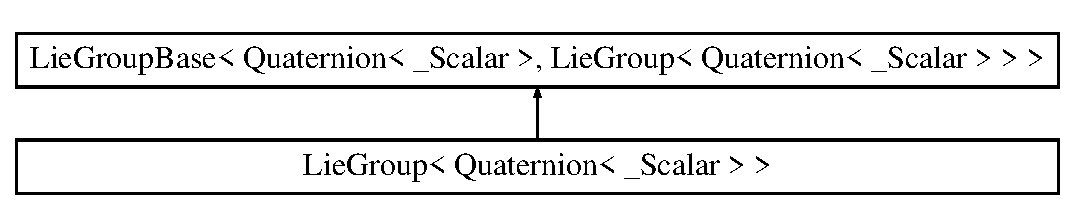
\includegraphics[height=2.000000cm]{class_lie_group_3_01_quaternion_3_01___scalar_01_4_01_4}
\end{center}
\end{figure}
\subsection*{Public Types}
\begin{DoxyCompactItemize}
\item 
typedef \+\_\+\+Scalar \hyperlink{class_lie_group_3_01_quaternion_3_01___scalar_01_4_01_4_a5c9cc4f61c2a1870f44da7951225dc4e}{Scalar}
\item 
typedef internal\+::traits$<$ \hyperlink{class_lie_group}{Lie\+Group}$<$ Quaternion$<$ \hyperlink{class_lie_group_3_01_quaternion_3_01___scalar_01_4_01_4_a5c9cc4f61c2a1870f44da7951225dc4e}{Scalar} $>$ $>$ $>$\+::\hyperlink{class_lie_group_3_01_quaternion_3_01___scalar_01_4_01_4_a80504cfb3bcbf55c7d4c1e377ef9f782}{Coefficients} \hyperlink{class_lie_group_3_01_quaternion_3_01___scalar_01_4_01_4_a80504cfb3bcbf55c7d4c1e377ef9f782}{Coefficients}
\end{DoxyCompactItemize}
\subsection*{Public Member Functions}
\begin{DoxyCompactItemize}
\item 
\hyperlink{class_lie_group_3_01_quaternion_3_01___scalar_01_4_01_4_a0810d682a2a637aa77877e84695bc884}{Lie\+Group} ()
\item 
{\footnotesize template$<$class Other\+Derived $>$ }\\\hyperlink{class_lie_group_3_01_quaternion_3_01___scalar_01_4_01_4_a56d1bf6da37ec19a2e2857f5c982410a}{Lie\+Group} (const \hyperlink{class_lie_group_base}{Lie\+Group\+Base}$<$ typename \hyperlink{class_lie_group_base_a895bed679f100c71c6dcbfd5532635b0}{Base\+::\+Base\+Type}, Other\+Derived $>$ \&g)
\item 
E\+I\+G\+E\+N\+\_\+\+S\+T\+R\+O\+N\+G\+\_\+\+I\+N\+L\+I\+NE \hyperlink{class_lie_group_3_01_quaternion_3_01___scalar_01_4_01_4_a7126b500c3e732fd1eba547c03fdf34e}{Lie\+Group} (const \hyperlink{class_lie_group_3_01_quaternion_3_01___scalar_01_4_01_4_a80504cfb3bcbf55c7d4c1e377ef9f782}{Coefficients} \&g)
\item 
E\+I\+G\+E\+N\+\_\+\+S\+T\+R\+O\+N\+G\+\_\+\+I\+N\+L\+I\+NE \hyperlink{class_lie_group_3_01_quaternion_3_01___scalar_01_4_01_4_ab91fa6322f5c3573fcff1b27a3c55d6f}{Lie\+Group} (const Angle\+Axis$<$ \hyperlink{class_lie_group_3_01_quaternion_3_01___scalar_01_4_01_4_a5c9cc4f61c2a1870f44da7951225dc4e}{Scalar} $>$ \&aa)
\item 
{\footnotesize template$<$class Other\+Derived $>$ }\\\hyperlink{class_lie_group_3_01_quaternion_3_01___scalar_01_4_01_4_a0b505b5a4a7bc08f699a347b0ead4a4f}{Lie\+Group} (\hyperlink{class_lie_group_3_01_quaternion_3_01___scalar_01_4_01_4_a5c9cc4f61c2a1870f44da7951225dc4e}{Scalar} w, const Matrix\+Base$<$ Other\+Derived $>$ \&vec)
\item 
{\footnotesize template$<$typename Derived $>$ }\\\hyperlink{class_lie_group_3_01_quaternion_3_01___scalar_01_4_01_4_a19ea5d83094ec2d26d6e856d670b952d}{Lie\+Group} (const Matrix\+Base$<$ Derived $>$ \&other)
\item 
{\footnotesize template$<$typename Derived $>$ }\\\hyperlink{class_lie_group_3_01_quaternion_3_01___scalar_01_4_01_4_ada8f3063710d6ef0737a43f0a6f55af2}{Lie\+Group} (const Matrix$<$ \hyperlink{class_lie_group_3_01_quaternion_3_01___scalar_01_4_01_4_a5c9cc4f61c2a1870f44da7951225dc4e}{Scalar}, 4, 1 $>$ \&other)
\item 
\hyperlink{class_lie_group_3_01_quaternion_3_01___scalar_01_4_01_4_ae14ff68d6699e47d32bedc863725ce40}{Lie\+Group} (\hyperlink{class_lie_group_3_01_quaternion_3_01___scalar_01_4_01_4_a5c9cc4f61c2a1870f44da7951225dc4e}{Scalar} w, \hyperlink{class_lie_group_3_01_quaternion_3_01___scalar_01_4_01_4_a5c9cc4f61c2a1870f44da7951225dc4e}{Scalar} x, \hyperlink{class_lie_group_3_01_quaternion_3_01___scalar_01_4_01_4_a5c9cc4f61c2a1870f44da7951225dc4e}{Scalar} y, \hyperlink{class_lie_group_3_01_quaternion_3_01___scalar_01_4_01_4_a5c9cc4f61c2a1870f44da7951225dc4e}{Scalar} z)
\item 
\hyperlink{class_lie_group_3_01_quaternion_3_01___scalar_01_4_01_4_a6526f663ef495eab03b24a2a97ff6df2}{Lie\+Group} (\hyperlink{class_lie_group_3_01_quaternion_3_01___scalar_01_4_01_4_a5c9cc4f61c2a1870f44da7951225dc4e}{Scalar} w, const Matrix$<$ \hyperlink{class_lie_group_3_01_quaternion_3_01___scalar_01_4_01_4_a5c9cc4f61c2a1870f44da7951225dc4e}{Scalar}, 3, 1 $>$ \&v)
\item 
\hyperlink{class_lie_group_3_01_quaternion_3_01___scalar_01_4_01_4_a80504cfb3bcbf55c7d4c1e377ef9f782}{Coefficients} \& \hyperlink{class_lie_group_3_01_quaternion_3_01___scalar_01_4_01_4_aec4805ed17f1c1ce893bcfdd8776deb2}{get} ()
\item 
const \hyperlink{class_lie_group_3_01_quaternion_3_01___scalar_01_4_01_4_a80504cfb3bcbf55c7d4c1e377ef9f782}{Coefficients} \& \hyperlink{class_lie_group_3_01_quaternion_3_01___scalar_01_4_01_4_a81591117317bb7817883ce137bae5ec3}{get} () const
\end{DoxyCompactItemize}
\subsection*{Protected Types}
\begin{DoxyCompactItemize}
\item 
typedef \hyperlink{class_lie_group_base}{Lie\+Group\+Base}$<$ Quaternion$<$ \+\_\+\+Scalar $>$, \hyperlink{class_lie_group}{Lie\+Group}$<$ Quaternion$<$ \+\_\+\+Scalar $>$ $>$ $>$ \hyperlink{class_lie_group_3_01_quaternion_3_01___scalar_01_4_01_4_a08877e48ca8072baeeed20cedb358b8c}{Base}
\end{DoxyCompactItemize}
\subsection*{Protected Attributes}
\begin{DoxyCompactItemize}
\item 
\hyperlink{class_lie_group_3_01_quaternion_3_01___scalar_01_4_01_4_a80504cfb3bcbf55c7d4c1e377ef9f782}{Coefficients} \hyperlink{class_lie_group_3_01_quaternion_3_01___scalar_01_4_01_4_a8bf670b6608a4fa3139244167131925f}{m\+\_\+coeffs}
\end{DoxyCompactItemize}
\subsection*{Additional Inherited Members}


\subsection{Detailed Description}
\subsubsection*{template$<$typename \+\_\+\+Scalar$>$\newline
class Lie\+Group$<$ Quaternion$<$ \+\_\+\+Scalar $>$ $>$}

Class for S\+O(3) Lie Group. 

Definition of Lie\+Group$<$\+Quaternion$>$


\begin{DoxyTemplParams}{Template Parameters}
{\em \+\_\+\+Scalar} & the type of the underlying quaternion\\
\hline
\end{DoxyTemplParams}
This class is a specialization of \hyperlink{class_lie_group}{Lie\+Group}. It adds specific constructor for S\+O(3).

\begin{DoxySeeAlso}{See also}
The methods are defined in \hyperlink{class_lie_group_base}{Lie\+Group\+Base} 
\end{DoxySeeAlso}


Definition at line 230 of file Lie\+Group\+\_\+\+S\+O3.\+h.



\subsection{Member Typedef Documentation}
\hypertarget{class_lie_group_3_01_quaternion_3_01___scalar_01_4_01_4_a08877e48ca8072baeeed20cedb358b8c}{}\label{class_lie_group_3_01_quaternion_3_01___scalar_01_4_01_4_a08877e48ca8072baeeed20cedb358b8c} 
\index{Lie\+Group$<$ Quaternion$<$ \+\_\+\+Scalar $>$ $>$@{Lie\+Group$<$ Quaternion$<$ \+\_\+\+Scalar $>$ $>$}!Base@{Base}}
\index{Base@{Base}!Lie\+Group$<$ Quaternion$<$ \+\_\+\+Scalar $>$ $>$@{Lie\+Group$<$ Quaternion$<$ \+\_\+\+Scalar $>$ $>$}}
\subsubsection{\texorpdfstring{Base}{Base}}
{\footnotesize\ttfamily template$<$typename \+\_\+\+Scalar $>$ \\
typedef \hyperlink{class_lie_group_base}{Lie\+Group\+Base}$<$Quaternion$<$\+\_\+\+Scalar$>$, \hyperlink{class_lie_group}{Lie\+Group}$<$Quaternion$<$\+\_\+\+Scalar$>$ $>$ $>$ \hyperlink{class_lie_group}{Lie\+Group}$<$ Quaternion$<$ \+\_\+\+Scalar $>$ $>$\+::\hyperlink{class_lie_group_3_01_quaternion_3_01___scalar_01_4_01_4_a08877e48ca8072baeeed20cedb358b8c}{Base}\hspace{0.3cm}{\ttfamily [protected]}}

The inherited class 

Definition at line 235 of file Lie\+Group\+\_\+\+S\+O3.\+h.

\hypertarget{class_lie_group_3_01_quaternion_3_01___scalar_01_4_01_4_a80504cfb3bcbf55c7d4c1e377ef9f782}{}\label{class_lie_group_3_01_quaternion_3_01___scalar_01_4_01_4_a80504cfb3bcbf55c7d4c1e377ef9f782} 
\index{Lie\+Group$<$ Quaternion$<$ \+\_\+\+Scalar $>$ $>$@{Lie\+Group$<$ Quaternion$<$ \+\_\+\+Scalar $>$ $>$}!Coefficients@{Coefficients}}
\index{Coefficients@{Coefficients}!Lie\+Group$<$ Quaternion$<$ \+\_\+\+Scalar $>$ $>$@{Lie\+Group$<$ Quaternion$<$ \+\_\+\+Scalar $>$ $>$}}
\subsubsection{\texorpdfstring{Coefficients}{Coefficients}}
{\footnotesize\ttfamily template$<$typename \+\_\+\+Scalar $>$ \\
typedef internal\+::traits$<$\hyperlink{class_lie_group}{Lie\+Group}$<$Quaternion$<$\hyperlink{class_lie_group_3_01_quaternion_3_01___scalar_01_4_01_4_a5c9cc4f61c2a1870f44da7951225dc4e}{Scalar}$>$ $>$ $>$\+::\hyperlink{class_lie_group_3_01_quaternion_3_01___scalar_01_4_01_4_a80504cfb3bcbf55c7d4c1e377ef9f782}{Coefficients} \hyperlink{class_lie_group}{Lie\+Group}$<$ Quaternion$<$ \+\_\+\+Scalar $>$ $>$\+::\hyperlink{class_lie_group_3_01_quaternion_3_01___scalar_01_4_01_4_a80504cfb3bcbf55c7d4c1e377ef9f782}{Coefficients}}

the stored coefficients 

Definition at line 240 of file Lie\+Group\+\_\+\+S\+O3.\+h.

\hypertarget{class_lie_group_3_01_quaternion_3_01___scalar_01_4_01_4_a5c9cc4f61c2a1870f44da7951225dc4e}{}\label{class_lie_group_3_01_quaternion_3_01___scalar_01_4_01_4_a5c9cc4f61c2a1870f44da7951225dc4e} 
\index{Lie\+Group$<$ Quaternion$<$ \+\_\+\+Scalar $>$ $>$@{Lie\+Group$<$ Quaternion$<$ \+\_\+\+Scalar $>$ $>$}!Scalar@{Scalar}}
\index{Scalar@{Scalar}!Lie\+Group$<$ Quaternion$<$ \+\_\+\+Scalar $>$ $>$@{Lie\+Group$<$ Quaternion$<$ \+\_\+\+Scalar $>$ $>$}}
\subsubsection{\texorpdfstring{Scalar}{Scalar}}
{\footnotesize\ttfamily template$<$typename \+\_\+\+Scalar $>$ \\
typedef \+\_\+\+Scalar \hyperlink{class_lie_group}{Lie\+Group}$<$ Quaternion$<$ \+\_\+\+Scalar $>$ $>$\+::\hyperlink{class_lie_group_3_01_quaternion_3_01___scalar_01_4_01_4_a5c9cc4f61c2a1870f44da7951225dc4e}{Scalar}}

The coefficients type 

Definition at line 238 of file Lie\+Group\+\_\+\+S\+O3.\+h.



\subsection{Constructor \& Destructor Documentation}
\hypertarget{class_lie_group_3_01_quaternion_3_01___scalar_01_4_01_4_a0810d682a2a637aa77877e84695bc884}{}\label{class_lie_group_3_01_quaternion_3_01___scalar_01_4_01_4_a0810d682a2a637aa77877e84695bc884} 
\index{Lie\+Group$<$ Quaternion$<$ \+\_\+\+Scalar $>$ $>$@{Lie\+Group$<$ Quaternion$<$ \+\_\+\+Scalar $>$ $>$}!Lie\+Group@{Lie\+Group}}
\index{Lie\+Group@{Lie\+Group}!Lie\+Group$<$ Quaternion$<$ \+\_\+\+Scalar $>$ $>$@{Lie\+Group$<$ Quaternion$<$ \+\_\+\+Scalar $>$ $>$}}
\subsubsection{\texorpdfstring{Lie\+Group()}{LieGroup()}\hspace{0.1cm}{\footnotesize\ttfamily [1/9]}}
{\footnotesize\ttfamily template$<$typename \+\_\+\+Scalar $>$ \\
\hyperlink{class_lie_group}{Lie\+Group}$<$ Quaternion$<$ \+\_\+\+Scalar $>$ $>$\+::\hyperlink{class_lie_group}{Lie\+Group} (\begin{DoxyParamCaption}{ }\end{DoxyParamCaption})\hspace{0.3cm}{\ttfamily [inline]}}

Default constructor 

Definition at line 245 of file Lie\+Group\+\_\+\+S\+O3.\+h.

\hypertarget{class_lie_group_3_01_quaternion_3_01___scalar_01_4_01_4_a56d1bf6da37ec19a2e2857f5c982410a}{}\label{class_lie_group_3_01_quaternion_3_01___scalar_01_4_01_4_a56d1bf6da37ec19a2e2857f5c982410a} 
\index{Lie\+Group$<$ Quaternion$<$ \+\_\+\+Scalar $>$ $>$@{Lie\+Group$<$ Quaternion$<$ \+\_\+\+Scalar $>$ $>$}!Lie\+Group@{Lie\+Group}}
\index{Lie\+Group@{Lie\+Group}!Lie\+Group$<$ Quaternion$<$ \+\_\+\+Scalar $>$ $>$@{Lie\+Group$<$ Quaternion$<$ \+\_\+\+Scalar $>$ $>$}}
\subsubsection{\texorpdfstring{Lie\+Group()}{LieGroup()}\hspace{0.1cm}{\footnotesize\ttfamily [2/9]}}
{\footnotesize\ttfamily template$<$typename \+\_\+\+Scalar $>$ \\
template$<$class Other\+Derived $>$ \\
\hyperlink{class_lie_group}{Lie\+Group}$<$ Quaternion$<$ \+\_\+\+Scalar $>$ $>$\+::\hyperlink{class_lie_group}{Lie\+Group} (\begin{DoxyParamCaption}\item[{const \hyperlink{class_lie_group_base}{Lie\+Group\+Base}$<$ typename \hyperlink{class_lie_group_base_a895bed679f100c71c6dcbfd5532635b0}{Base\+::\+Base\+Type}, Other\+Derived $>$ \&}]{g }\end{DoxyParamCaption})\hspace{0.3cm}{\ttfamily [inline]}}

Copy constructor 

Definition at line 247 of file Lie\+Group\+\_\+\+S\+O3.\+h.

\hypertarget{class_lie_group_3_01_quaternion_3_01___scalar_01_4_01_4_a7126b500c3e732fd1eba547c03fdf34e}{}\label{class_lie_group_3_01_quaternion_3_01___scalar_01_4_01_4_a7126b500c3e732fd1eba547c03fdf34e} 
\index{Lie\+Group$<$ Quaternion$<$ \+\_\+\+Scalar $>$ $>$@{Lie\+Group$<$ Quaternion$<$ \+\_\+\+Scalar $>$ $>$}!Lie\+Group@{Lie\+Group}}
\index{Lie\+Group@{Lie\+Group}!Lie\+Group$<$ Quaternion$<$ \+\_\+\+Scalar $>$ $>$@{Lie\+Group$<$ Quaternion$<$ \+\_\+\+Scalar $>$ $>$}}
\subsubsection{\texorpdfstring{Lie\+Group()}{LieGroup()}\hspace{0.1cm}{\footnotesize\ttfamily [3/9]}}
{\footnotesize\ttfamily template$<$typename \+\_\+\+Scalar $>$ \\
E\+I\+G\+E\+N\+\_\+\+S\+T\+R\+O\+N\+G\+\_\+\+I\+N\+L\+I\+NE \hyperlink{class_lie_group}{Lie\+Group}$<$ Quaternion$<$ \+\_\+\+Scalar $>$ $>$\+::\hyperlink{class_lie_group}{Lie\+Group} (\begin{DoxyParamCaption}\item[{const \hyperlink{class_lie_group_3_01_quaternion_3_01___scalar_01_4_01_4_a80504cfb3bcbf55c7d4c1e377ef9f782}{Coefficients} \&}]{g }\end{DoxyParamCaption})\hspace{0.3cm}{\ttfamily [inline]}}

Copy constructor Copy constructor 

Definition at line 251 of file Lie\+Group\+\_\+\+S\+O3.\+h.

\hypertarget{class_lie_group_3_01_quaternion_3_01___scalar_01_4_01_4_ab91fa6322f5c3573fcff1b27a3c55d6f}{}\label{class_lie_group_3_01_quaternion_3_01___scalar_01_4_01_4_ab91fa6322f5c3573fcff1b27a3c55d6f} 
\index{Lie\+Group$<$ Quaternion$<$ \+\_\+\+Scalar $>$ $>$@{Lie\+Group$<$ Quaternion$<$ \+\_\+\+Scalar $>$ $>$}!Lie\+Group@{Lie\+Group}}
\index{Lie\+Group@{Lie\+Group}!Lie\+Group$<$ Quaternion$<$ \+\_\+\+Scalar $>$ $>$@{Lie\+Group$<$ Quaternion$<$ \+\_\+\+Scalar $>$ $>$}}
\subsubsection{\texorpdfstring{Lie\+Group()}{LieGroup()}\hspace{0.1cm}{\footnotesize\ttfamily [4/9]}}
{\footnotesize\ttfamily template$<$typename \+\_\+\+Scalar $>$ \\
E\+I\+G\+E\+N\+\_\+\+S\+T\+R\+O\+N\+G\+\_\+\+I\+N\+L\+I\+NE \hyperlink{class_lie_group}{Lie\+Group}$<$ Quaternion$<$ \+\_\+\+Scalar $>$ $>$\+::\hyperlink{class_lie_group}{Lie\+Group} (\begin{DoxyParamCaption}\item[{const Angle\+Axis$<$ \hyperlink{class_lie_group_3_01_quaternion_3_01___scalar_01_4_01_4_a5c9cc4f61c2a1870f44da7951225dc4e}{Scalar} $>$ \&}]{aa }\end{DoxyParamCaption})\hspace{0.3cm}{\ttfamily [inline]}}



Definition at line 252 of file Lie\+Group\+\_\+\+S\+O3.\+h.

\hypertarget{class_lie_group_3_01_quaternion_3_01___scalar_01_4_01_4_a0b505b5a4a7bc08f699a347b0ead4a4f}{}\label{class_lie_group_3_01_quaternion_3_01___scalar_01_4_01_4_a0b505b5a4a7bc08f699a347b0ead4a4f} 
\index{Lie\+Group$<$ Quaternion$<$ \+\_\+\+Scalar $>$ $>$@{Lie\+Group$<$ Quaternion$<$ \+\_\+\+Scalar $>$ $>$}!Lie\+Group@{Lie\+Group}}
\index{Lie\+Group@{Lie\+Group}!Lie\+Group$<$ Quaternion$<$ \+\_\+\+Scalar $>$ $>$@{Lie\+Group$<$ Quaternion$<$ \+\_\+\+Scalar $>$ $>$}}
\subsubsection{\texorpdfstring{Lie\+Group()}{LieGroup()}\hspace{0.1cm}{\footnotesize\ttfamily [5/9]}}
{\footnotesize\ttfamily template$<$typename \+\_\+\+Scalar $>$ \\
template$<$class Other\+Derived $>$ \\
\hyperlink{class_lie_group}{Lie\+Group}$<$ Quaternion$<$ \+\_\+\+Scalar $>$ $>$\+::\hyperlink{class_lie_group}{Lie\+Group} (\begin{DoxyParamCaption}\item[{\hyperlink{class_lie_group_3_01_quaternion_3_01___scalar_01_4_01_4_a5c9cc4f61c2a1870f44da7951225dc4e}{Scalar}}]{w,  }\item[{const Matrix\+Base$<$ Other\+Derived $>$ \&}]{vec }\end{DoxyParamCaption})\hspace{0.3cm}{\ttfamily [inline]}}

Constructs a element of S\+O(3) from a scalar {\ttfamily w} and a vector {\ttfamily vec}. The underlying quaternion is initialized with w, vec\mbox{[}0\mbox{]}, vec\mbox{[}1\mbox{]}, vec\mbox{[}2\mbox{]} 

Definition at line 255 of file Lie\+Group\+\_\+\+S\+O3.\+h.

\hypertarget{class_lie_group_3_01_quaternion_3_01___scalar_01_4_01_4_a19ea5d83094ec2d26d6e856d670b952d}{}\label{class_lie_group_3_01_quaternion_3_01___scalar_01_4_01_4_a19ea5d83094ec2d26d6e856d670b952d} 
\index{Lie\+Group$<$ Quaternion$<$ \+\_\+\+Scalar $>$ $>$@{Lie\+Group$<$ Quaternion$<$ \+\_\+\+Scalar $>$ $>$}!Lie\+Group@{Lie\+Group}}
\index{Lie\+Group@{Lie\+Group}!Lie\+Group$<$ Quaternion$<$ \+\_\+\+Scalar $>$ $>$@{Lie\+Group$<$ Quaternion$<$ \+\_\+\+Scalar $>$ $>$}}
\subsubsection{\texorpdfstring{Lie\+Group()}{LieGroup()}\hspace{0.1cm}{\footnotesize\ttfamily [6/9]}}
{\footnotesize\ttfamily template$<$typename \+\_\+\+Scalar $>$ \\
template$<$typename Derived $>$ \\
\hyperlink{class_lie_group}{Lie\+Group}$<$ Quaternion$<$ \+\_\+\+Scalar $>$ $>$\+::\hyperlink{class_lie_group}{Lie\+Group} (\begin{DoxyParamCaption}\item[{const Matrix\+Base$<$ Derived $>$ \&}]{other }\end{DoxyParamCaption})\hspace{0.3cm}{\ttfamily [inline]}, {\ttfamily [explicit]}}

Intialize from rotation matrix 

Definition at line 263 of file Lie\+Group\+\_\+\+S\+O3.\+h.

\hypertarget{class_lie_group_3_01_quaternion_3_01___scalar_01_4_01_4_ada8f3063710d6ef0737a43f0a6f55af2}{}\label{class_lie_group_3_01_quaternion_3_01___scalar_01_4_01_4_ada8f3063710d6ef0737a43f0a6f55af2} 
\index{Lie\+Group$<$ Quaternion$<$ \+\_\+\+Scalar $>$ $>$@{Lie\+Group$<$ Quaternion$<$ \+\_\+\+Scalar $>$ $>$}!Lie\+Group@{Lie\+Group}}
\index{Lie\+Group@{Lie\+Group}!Lie\+Group$<$ Quaternion$<$ \+\_\+\+Scalar $>$ $>$@{Lie\+Group$<$ Quaternion$<$ \+\_\+\+Scalar $>$ $>$}}
\subsubsection{\texorpdfstring{Lie\+Group()}{LieGroup()}\hspace{0.1cm}{\footnotesize\ttfamily [7/9]}}
{\footnotesize\ttfamily template$<$typename \+\_\+\+Scalar $>$ \\
template$<$typename Derived $>$ \\
\hyperlink{class_lie_group}{Lie\+Group}$<$ Quaternion$<$ \+\_\+\+Scalar $>$ $>$\+::\hyperlink{class_lie_group}{Lie\+Group} (\begin{DoxyParamCaption}\item[{const Matrix$<$ \hyperlink{class_lie_group_3_01_quaternion_3_01___scalar_01_4_01_4_a5c9cc4f61c2a1870f44da7951225dc4e}{Scalar}, 4, 1 $>$ \&}]{other }\end{DoxyParamCaption})\hspace{0.3cm}{\ttfamily [inline]}, {\ttfamily [explicit]}}



Definition at line 266 of file Lie\+Group\+\_\+\+S\+O3.\+h.

\hypertarget{class_lie_group_3_01_quaternion_3_01___scalar_01_4_01_4_ae14ff68d6699e47d32bedc863725ce40}{}\label{class_lie_group_3_01_quaternion_3_01___scalar_01_4_01_4_ae14ff68d6699e47d32bedc863725ce40} 
\index{Lie\+Group$<$ Quaternion$<$ \+\_\+\+Scalar $>$ $>$@{Lie\+Group$<$ Quaternion$<$ \+\_\+\+Scalar $>$ $>$}!Lie\+Group@{Lie\+Group}}
\index{Lie\+Group@{Lie\+Group}!Lie\+Group$<$ Quaternion$<$ \+\_\+\+Scalar $>$ $>$@{Lie\+Group$<$ Quaternion$<$ \+\_\+\+Scalar $>$ $>$}}
\subsubsection{\texorpdfstring{Lie\+Group()}{LieGroup()}\hspace{0.1cm}{\footnotesize\ttfamily [8/9]}}
{\footnotesize\ttfamily template$<$typename \+\_\+\+Scalar $>$ \\
\hyperlink{class_lie_group}{Lie\+Group}$<$ Quaternion$<$ \+\_\+\+Scalar $>$ $>$\+::\hyperlink{class_lie_group}{Lie\+Group} (\begin{DoxyParamCaption}\item[{\hyperlink{class_lie_group_3_01_quaternion_3_01___scalar_01_4_01_4_a5c9cc4f61c2a1870f44da7951225dc4e}{Scalar}}]{w,  }\item[{\hyperlink{class_lie_group_3_01_quaternion_3_01___scalar_01_4_01_4_a5c9cc4f61c2a1870f44da7951225dc4e}{Scalar}}]{x,  }\item[{\hyperlink{class_lie_group_3_01_quaternion_3_01___scalar_01_4_01_4_a5c9cc4f61c2a1870f44da7951225dc4e}{Scalar}}]{y,  }\item[{\hyperlink{class_lie_group_3_01_quaternion_3_01___scalar_01_4_01_4_a5c9cc4f61c2a1870f44da7951225dc4e}{Scalar}}]{z }\end{DoxyParamCaption})\hspace{0.3cm}{\ttfamily [inline]}}

Constructs and initializes the quaternion $ w+xi+yj+zk $ from its four coefficients {\itshape w}, {\itshape x}, {\itshape y} and {\itshape z}.

\begin{DoxyWarning}{Warning}
Note the order of the arguments\+: the real {\itshape w} coefficient first, while internally the coefficients are stored in the following order\+: \mbox{[}{\ttfamily x}, {\ttfamily y}, {\ttfamily z}, {\ttfamily w}\mbox{]} 
\end{DoxyWarning}


Definition at line 275 of file Lie\+Group\+\_\+\+S\+O3.\+h.

\hypertarget{class_lie_group_3_01_quaternion_3_01___scalar_01_4_01_4_a6526f663ef495eab03b24a2a97ff6df2}{}\label{class_lie_group_3_01_quaternion_3_01___scalar_01_4_01_4_a6526f663ef495eab03b24a2a97ff6df2} 
\index{Lie\+Group$<$ Quaternion$<$ \+\_\+\+Scalar $>$ $>$@{Lie\+Group$<$ Quaternion$<$ \+\_\+\+Scalar $>$ $>$}!Lie\+Group@{Lie\+Group}}
\index{Lie\+Group@{Lie\+Group}!Lie\+Group$<$ Quaternion$<$ \+\_\+\+Scalar $>$ $>$@{Lie\+Group$<$ Quaternion$<$ \+\_\+\+Scalar $>$ $>$}}
\subsubsection{\texorpdfstring{Lie\+Group()}{LieGroup()}\hspace{0.1cm}{\footnotesize\ttfamily [9/9]}}
{\footnotesize\ttfamily template$<$typename \+\_\+\+Scalar $>$ \\
\hyperlink{class_lie_group}{Lie\+Group}$<$ Quaternion$<$ \+\_\+\+Scalar $>$ $>$\+::\hyperlink{class_lie_group}{Lie\+Group} (\begin{DoxyParamCaption}\item[{\hyperlink{class_lie_group_3_01_quaternion_3_01___scalar_01_4_01_4_a5c9cc4f61c2a1870f44da7951225dc4e}{Scalar}}]{w,  }\item[{const Matrix$<$ \hyperlink{class_lie_group_3_01_quaternion_3_01___scalar_01_4_01_4_a5c9cc4f61c2a1870f44da7951225dc4e}{Scalar}, 3, 1 $>$ \&}]{v }\end{DoxyParamCaption})\hspace{0.3cm}{\ttfamily [inline]}}



Definition at line 276 of file Lie\+Group\+\_\+\+S\+O3.\+h.



\subsection{Member Function Documentation}
\hypertarget{class_lie_group_3_01_quaternion_3_01___scalar_01_4_01_4_aec4805ed17f1c1ce893bcfdd8776deb2}{}\label{class_lie_group_3_01_quaternion_3_01___scalar_01_4_01_4_aec4805ed17f1c1ce893bcfdd8776deb2} 
\index{Lie\+Group$<$ Quaternion$<$ \+\_\+\+Scalar $>$ $>$@{Lie\+Group$<$ Quaternion$<$ \+\_\+\+Scalar $>$ $>$}!get@{get}}
\index{get@{get}!Lie\+Group$<$ Quaternion$<$ \+\_\+\+Scalar $>$ $>$@{Lie\+Group$<$ Quaternion$<$ \+\_\+\+Scalar $>$ $>$}}
\subsubsection{\texorpdfstring{get()}{get()}\hspace{0.1cm}{\footnotesize\ttfamily [1/2]}}
{\footnotesize\ttfamily template$<$typename \+\_\+\+Scalar $>$ \\
\hyperlink{class_lie_group_3_01_quaternion_3_01___scalar_01_4_01_4_a80504cfb3bcbf55c7d4c1e377ef9f782}{Coefficients}\& \hyperlink{class_lie_group}{Lie\+Group}$<$ Quaternion$<$ \+\_\+\+Scalar $>$ $>$\+::get (\begin{DoxyParamCaption}{ }\end{DoxyParamCaption})\hspace{0.3cm}{\ttfamily [inline]}}

\begin{DoxyReturn}{Returns}
The stored coefficients 
\end{DoxyReturn}


Definition at line 279 of file Lie\+Group\+\_\+\+S\+O3.\+h.

\hypertarget{class_lie_group_3_01_quaternion_3_01___scalar_01_4_01_4_a81591117317bb7817883ce137bae5ec3}{}\label{class_lie_group_3_01_quaternion_3_01___scalar_01_4_01_4_a81591117317bb7817883ce137bae5ec3} 
\index{Lie\+Group$<$ Quaternion$<$ \+\_\+\+Scalar $>$ $>$@{Lie\+Group$<$ Quaternion$<$ \+\_\+\+Scalar $>$ $>$}!get@{get}}
\index{get@{get}!Lie\+Group$<$ Quaternion$<$ \+\_\+\+Scalar $>$ $>$@{Lie\+Group$<$ Quaternion$<$ \+\_\+\+Scalar $>$ $>$}}
\subsubsection{\texorpdfstring{get()}{get()}\hspace{0.1cm}{\footnotesize\ttfamily [2/2]}}
{\footnotesize\ttfamily template$<$typename \+\_\+\+Scalar $>$ \\
const \hyperlink{class_lie_group_3_01_quaternion_3_01___scalar_01_4_01_4_a80504cfb3bcbf55c7d4c1e377ef9f782}{Coefficients}\& \hyperlink{class_lie_group}{Lie\+Group}$<$ Quaternion$<$ \+\_\+\+Scalar $>$ $>$\+::get (\begin{DoxyParamCaption}{ }\end{DoxyParamCaption}) const\hspace{0.3cm}{\ttfamily [inline]}}

\begin{DoxyReturn}{Returns}
The read-\/only access to the stored coefficients 
\end{DoxyReturn}


Definition at line 281 of file Lie\+Group\+\_\+\+S\+O3.\+h.



\subsection{Member Data Documentation}
\hypertarget{class_lie_group_3_01_quaternion_3_01___scalar_01_4_01_4_a8bf670b6608a4fa3139244167131925f}{}\label{class_lie_group_3_01_quaternion_3_01___scalar_01_4_01_4_a8bf670b6608a4fa3139244167131925f} 
\index{Lie\+Group$<$ Quaternion$<$ \+\_\+\+Scalar $>$ $>$@{Lie\+Group$<$ Quaternion$<$ \+\_\+\+Scalar $>$ $>$}!m\+\_\+coeffs@{m\+\_\+coeffs}}
\index{m\+\_\+coeffs@{m\+\_\+coeffs}!Lie\+Group$<$ Quaternion$<$ \+\_\+\+Scalar $>$ $>$@{Lie\+Group$<$ Quaternion$<$ \+\_\+\+Scalar $>$ $>$}}
\subsubsection{\texorpdfstring{m\+\_\+coeffs}{m\_coeffs}}
{\footnotesize\ttfamily template$<$typename \+\_\+\+Scalar $>$ \\
\hyperlink{class_lie_group_3_01_quaternion_3_01___scalar_01_4_01_4_a80504cfb3bcbf55c7d4c1e377ef9f782}{Coefficients} \hyperlink{class_lie_group}{Lie\+Group}$<$ Quaternion$<$ \+\_\+\+Scalar $>$ $>$\+::m\+\_\+coeffs\hspace{0.3cm}{\ttfamily [protected]}}

The wrapped coefficients 

Definition at line 285 of file Lie\+Group\+\_\+\+S\+O3.\+h.



The documentation for this class was generated from the following file\+:\begin{DoxyCompactItemize}
\item 
/\+Users/\+Ryan/\+Code/codyco-\/superbuild/libraries/\+Eigen\+Lgsm/unsupported/\+Eigen/src/\+Lgsm/\hyperlink{_lie_group___s_o3_8h}{Lie\+Group\+\_\+\+S\+O3.\+h}\end{DoxyCompactItemize}

\hypertarget{structinternal_1_1liegroup___s_e3__base__assign__impl}{}\section{internal\+:\+:liegroup\+\_\+\+S\+E3\+\_\+base\+\_\+assign\+\_\+impl$<$ Other, Other\+Rows, Other\+Cols $>$ Struct Template Reference}
\label{structinternal_1_1liegroup___s_e3__base__assign__impl}\index{internal\+::liegroup\+\_\+\+S\+E3\+\_\+base\+\_\+assign\+\_\+impl$<$ Other, Other\+Rows, Other\+Cols $>$@{internal\+::liegroup\+\_\+\+S\+E3\+\_\+base\+\_\+assign\+\_\+impl$<$ Other, Other\+Rows, Other\+Cols $>$}}


{\ttfamily \#include $<$Lie\+Group\+\_\+\+S\+E3.\+h$>$}



\subsection{Detailed Description}
\subsubsection*{template$<$typename Other, int Other\+Rows = Other\+::\+Rows\+At\+Compile\+Time, int Other\+Cols = Other\+::\+Cols\+At\+Compile\+Time$>$\newline
struct internal\+::liegroup\+\_\+\+S\+E3\+\_\+base\+\_\+assign\+\_\+impl$<$ Other, Other\+Rows, Other\+Cols $>$}



Definition at line 17 of file Lie\+Group\+\_\+\+S\+E3.\+h.



The documentation for this struct was generated from the following file\+:\begin{DoxyCompactItemize}
\item 
/\+Users/\+Ryan/\+Code/codyco-\/superbuild/libraries/\+Eigen\+Lgsm/unsupported/\+Eigen/src/\+Lgsm/\hyperlink{_lie_group___s_e3_8h}{Lie\+Group\+\_\+\+S\+E3.\+h}\end{DoxyCompactItemize}

\hypertarget{structinternal_1_1liegroup___s_e3__base__assign__impl_3_01_other_00_013_00_011_01_4}{}\section{internal\+:\+:liegroup\+\_\+\+S\+E3\+\_\+base\+\_\+assign\+\_\+impl$<$ Other, 3, 1 $>$ Struct Template Reference}
\label{structinternal_1_1liegroup___s_e3__base__assign__impl_3_01_other_00_013_00_011_01_4}\index{internal\+::liegroup\+\_\+\+S\+E3\+\_\+base\+\_\+assign\+\_\+impl$<$ Other, 3, 1 $>$@{internal\+::liegroup\+\_\+\+S\+E3\+\_\+base\+\_\+assign\+\_\+impl$<$ Other, 3, 1 $>$}}


{\ttfamily \#include $<$Lie\+Group\+\_\+\+S\+E3.\+h$>$}

\subsection*{Public Types}
\begin{DoxyCompactItemize}
\item 
typedef Other\+::\+Scalar \hyperlink{structinternal_1_1liegroup___s_e3__base__assign__impl_3_01_other_00_013_00_011_01_4_aef78132c5f1f66237af2dcf4873a24d0}{Scalar}
\end{DoxyCompactItemize}
\subsection*{Static Public Member Functions}
\begin{DoxyCompactItemize}
\item 
{\footnotesize template$<$class Derived $>$ }\\static void \hyperlink{structinternal_1_1liegroup___s_e3__base__assign__impl_3_01_other_00_013_00_011_01_4_aac0ef6a07b1f6e3fe0f550c85edff934}{run} (\hyperlink{class_lie_group_base}{Lie\+Group\+Base}$<$ Array$<$ typename internal\+::traits$<$ Derived $>$\+::\hyperlink{structinternal_1_1liegroup___s_e3__base__assign__impl_3_01_other_00_013_00_011_01_4_aef78132c5f1f66237af2dcf4873a24d0}{Scalar}, 7, 1 $>$, Derived $>$ \&q, const Other \&vec)
\end{DoxyCompactItemize}


\subsection{Detailed Description}
\subsubsection*{template$<$typename Other$>$\newline
struct internal\+::liegroup\+\_\+\+S\+E3\+\_\+base\+\_\+assign\+\_\+impl$<$ Other, 3, 1 $>$}



Definition at line 372 of file Lie\+Group\+\_\+\+S\+E3.\+h.



\subsection{Member Typedef Documentation}
\hypertarget{structinternal_1_1liegroup___s_e3__base__assign__impl_3_01_other_00_013_00_011_01_4_aef78132c5f1f66237af2dcf4873a24d0}{}\label{structinternal_1_1liegroup___s_e3__base__assign__impl_3_01_other_00_013_00_011_01_4_aef78132c5f1f66237af2dcf4873a24d0} 
\index{internal\+::liegroup\+\_\+\+S\+E3\+\_\+base\+\_\+assign\+\_\+impl$<$ Other, 3, 1 $>$@{internal\+::liegroup\+\_\+\+S\+E3\+\_\+base\+\_\+assign\+\_\+impl$<$ Other, 3, 1 $>$}!Scalar@{Scalar}}
\index{Scalar@{Scalar}!internal\+::liegroup\+\_\+\+S\+E3\+\_\+base\+\_\+assign\+\_\+impl$<$ Other, 3, 1 $>$@{internal\+::liegroup\+\_\+\+S\+E3\+\_\+base\+\_\+assign\+\_\+impl$<$ Other, 3, 1 $>$}}
\subsubsection{\texorpdfstring{Scalar}{Scalar}}
{\footnotesize\ttfamily template$<$typename Other $>$ \\
typedef Other\+::\+Scalar \hyperlink{structinternal_1_1liegroup___s_e3__base__assign__impl}{internal\+::liegroup\+\_\+\+S\+E3\+\_\+base\+\_\+assign\+\_\+impl}$<$ Other, 3, 1 $>$\+::\hyperlink{structinternal_1_1liegroup___s_e3__base__assign__impl_3_01_other_00_013_00_011_01_4_aef78132c5f1f66237af2dcf4873a24d0}{Scalar}}



Definition at line 375 of file Lie\+Group\+\_\+\+S\+E3.\+h.



\subsection{Member Function Documentation}
\hypertarget{structinternal_1_1liegroup___s_e3__base__assign__impl_3_01_other_00_013_00_011_01_4_aac0ef6a07b1f6e3fe0f550c85edff934}{}\label{structinternal_1_1liegroup___s_e3__base__assign__impl_3_01_other_00_013_00_011_01_4_aac0ef6a07b1f6e3fe0f550c85edff934} 
\index{internal\+::liegroup\+\_\+\+S\+E3\+\_\+base\+\_\+assign\+\_\+impl$<$ Other, 3, 1 $>$@{internal\+::liegroup\+\_\+\+S\+E3\+\_\+base\+\_\+assign\+\_\+impl$<$ Other, 3, 1 $>$}!run@{run}}
\index{run@{run}!internal\+::liegroup\+\_\+\+S\+E3\+\_\+base\+\_\+assign\+\_\+impl$<$ Other, 3, 1 $>$@{internal\+::liegroup\+\_\+\+S\+E3\+\_\+base\+\_\+assign\+\_\+impl$<$ Other, 3, 1 $>$}}
\subsubsection{\texorpdfstring{run()}{run()}}
{\footnotesize\ttfamily template$<$typename Other $>$ \\
template$<$class Derived $>$ \\
static void \hyperlink{structinternal_1_1liegroup___s_e3__base__assign__impl}{internal\+::liegroup\+\_\+\+S\+E3\+\_\+base\+\_\+assign\+\_\+impl}$<$ Other, 3, 1 $>$\+::run (\begin{DoxyParamCaption}\item[{\hyperlink{class_lie_group_base}{Lie\+Group\+Base}$<$ Array$<$ typename internal\+::traits$<$ Derived $>$\+::\hyperlink{structinternal_1_1liegroup___s_e3__base__assign__impl_3_01_other_00_013_00_011_01_4_aef78132c5f1f66237af2dcf4873a24d0}{Scalar}, 7, 1 $>$, Derived $>$ \&}]{q,  }\item[{const Other \&}]{vec }\end{DoxyParamCaption})\hspace{0.3cm}{\ttfamily [inline]}, {\ttfamily [static]}}



Definition at line 376 of file Lie\+Group\+\_\+\+S\+E3.\+h.



The documentation for this struct was generated from the following file\+:\begin{DoxyCompactItemize}
\item 
/\+Users/\+Ryan/\+Code/codyco-\/superbuild/libraries/\+Eigen\+Lgsm/unsupported/\+Eigen/src/\+Lgsm/\hyperlink{_lie_group___s_e3_8h}{Lie\+Group\+\_\+\+S\+E3.\+h}\end{DoxyCompactItemize}

\hypertarget{structinternal_1_1liegroup___s_e3__base__assign__impl_3_01_other_00_014_00_014_01_4}{}\section{internal\+:\+:liegroup\+\_\+\+S\+E3\+\_\+base\+\_\+assign\+\_\+impl$<$ Other, 4, 4 $>$ Struct Template Reference}
\label{structinternal_1_1liegroup___s_e3__base__assign__impl_3_01_other_00_014_00_014_01_4}\index{internal\+::liegroup\+\_\+\+S\+E3\+\_\+base\+\_\+assign\+\_\+impl$<$ Other, 4, 4 $>$@{internal\+::liegroup\+\_\+\+S\+E3\+\_\+base\+\_\+assign\+\_\+impl$<$ Other, 4, 4 $>$}}


{\ttfamily \#include $<$Lie\+Group\+\_\+\+S\+E3.\+h$>$}

\subsection*{Public Types}
\begin{DoxyCompactItemize}
\item 
typedef Other\+::\+Scalar \hyperlink{structinternal_1_1liegroup___s_e3__base__assign__impl_3_01_other_00_014_00_014_01_4_a850deb96b6b52d92a8ae1e6d771b24be}{Scalar}
\end{DoxyCompactItemize}
\subsection*{Static Public Member Functions}
\begin{DoxyCompactItemize}
\item 
{\footnotesize template$<$class Derived $>$ }\\static void \hyperlink{structinternal_1_1liegroup___s_e3__base__assign__impl_3_01_other_00_014_00_014_01_4_a23f778b47ec9a8303bcb3ee52cc84c0f}{run} (\hyperlink{class_lie_group_base}{Lie\+Group\+Base}$<$ Array$<$ typename internal\+::traits$<$ Derived $>$\+::\hyperlink{structinternal_1_1liegroup___s_e3__base__assign__impl_3_01_other_00_014_00_014_01_4_a850deb96b6b52d92a8ae1e6d771b24be}{Scalar}, 7, 1 $>$, Derived $>$ \&q, const Other \&m)
\end{DoxyCompactItemize}


\subsection{Detailed Description}
\subsubsection*{template$<$typename Other$>$\newline
struct internal\+::liegroup\+\_\+\+S\+E3\+\_\+base\+\_\+assign\+\_\+impl$<$ Other, 4, 4 $>$}



Definition at line 359 of file Lie\+Group\+\_\+\+S\+E3.\+h.



\subsection{Member Typedef Documentation}
\hypertarget{structinternal_1_1liegroup___s_e3__base__assign__impl_3_01_other_00_014_00_014_01_4_a850deb96b6b52d92a8ae1e6d771b24be}{}\label{structinternal_1_1liegroup___s_e3__base__assign__impl_3_01_other_00_014_00_014_01_4_a850deb96b6b52d92a8ae1e6d771b24be} 
\index{internal\+::liegroup\+\_\+\+S\+E3\+\_\+base\+\_\+assign\+\_\+impl$<$ Other, 4, 4 $>$@{internal\+::liegroup\+\_\+\+S\+E3\+\_\+base\+\_\+assign\+\_\+impl$<$ Other, 4, 4 $>$}!Scalar@{Scalar}}
\index{Scalar@{Scalar}!internal\+::liegroup\+\_\+\+S\+E3\+\_\+base\+\_\+assign\+\_\+impl$<$ Other, 4, 4 $>$@{internal\+::liegroup\+\_\+\+S\+E3\+\_\+base\+\_\+assign\+\_\+impl$<$ Other, 4, 4 $>$}}
\subsubsection{\texorpdfstring{Scalar}{Scalar}}
{\footnotesize\ttfamily template$<$typename Other $>$ \\
typedef Other\+::\+Scalar \hyperlink{structinternal_1_1liegroup___s_e3__base__assign__impl}{internal\+::liegroup\+\_\+\+S\+E3\+\_\+base\+\_\+assign\+\_\+impl}$<$ Other, 4, 4 $>$\+::\hyperlink{structinternal_1_1liegroup___s_e3__base__assign__impl_3_01_other_00_014_00_014_01_4_a850deb96b6b52d92a8ae1e6d771b24be}{Scalar}}



Definition at line 362 of file Lie\+Group\+\_\+\+S\+E3.\+h.



\subsection{Member Function Documentation}
\hypertarget{structinternal_1_1liegroup___s_e3__base__assign__impl_3_01_other_00_014_00_014_01_4_a23f778b47ec9a8303bcb3ee52cc84c0f}{}\label{structinternal_1_1liegroup___s_e3__base__assign__impl_3_01_other_00_014_00_014_01_4_a23f778b47ec9a8303bcb3ee52cc84c0f} 
\index{internal\+::liegroup\+\_\+\+S\+E3\+\_\+base\+\_\+assign\+\_\+impl$<$ Other, 4, 4 $>$@{internal\+::liegroup\+\_\+\+S\+E3\+\_\+base\+\_\+assign\+\_\+impl$<$ Other, 4, 4 $>$}!run@{run}}
\index{run@{run}!internal\+::liegroup\+\_\+\+S\+E3\+\_\+base\+\_\+assign\+\_\+impl$<$ Other, 4, 4 $>$@{internal\+::liegroup\+\_\+\+S\+E3\+\_\+base\+\_\+assign\+\_\+impl$<$ Other, 4, 4 $>$}}
\subsubsection{\texorpdfstring{run()}{run()}}
{\footnotesize\ttfamily template$<$typename Other $>$ \\
template$<$class Derived $>$ \\
static void \hyperlink{structinternal_1_1liegroup___s_e3__base__assign__impl}{internal\+::liegroup\+\_\+\+S\+E3\+\_\+base\+\_\+assign\+\_\+impl}$<$ Other, 4, 4 $>$\+::run (\begin{DoxyParamCaption}\item[{\hyperlink{class_lie_group_base}{Lie\+Group\+Base}$<$ Array$<$ typename internal\+::traits$<$ Derived $>$\+::\hyperlink{structinternal_1_1liegroup___s_e3__base__assign__impl_3_01_other_00_014_00_014_01_4_a850deb96b6b52d92a8ae1e6d771b24be}{Scalar}, 7, 1 $>$, Derived $>$ \&}]{q,  }\item[{const Other \&}]{m }\end{DoxyParamCaption})\hspace{0.3cm}{\ttfamily [inline]}, {\ttfamily [static]}}



Definition at line 363 of file Lie\+Group\+\_\+\+S\+E3.\+h.



The documentation for this struct was generated from the following file\+:\begin{DoxyCompactItemize}
\item 
/\+Users/\+Ryan/\+Code/codyco-\/superbuild/libraries/\+Eigen\+Lgsm/unsupported/\+Eigen/src/\+Lgsm/\hyperlink{_lie_group___s_e3_8h}{Lie\+Group\+\_\+\+S\+E3.\+h}\end{DoxyCompactItemize}

\hypertarget{class_lie_group_base}{}\section{Lie\+Group\+Base$<$ G, Derived $>$ Class Template Reference}
\label{class_lie_group_base}\index{Lie\+Group\+Base$<$ G, Derived $>$@{Lie\+Group\+Base$<$ G, Derived $>$}}


Base class for all Lie Group class.  




{\ttfamily \#include $<$Lie\+Group.\+h$>$}

\subsection*{Public Types}
\begin{DoxyCompactItemize}
\item 
typedef Derived\+::\+Coefficients \hyperlink{class_lie_group_base_abb840873afd0a4f54f9ad4265e1d0095}{Coefficients}
\item 
typedef internal\+::traits$<$ Derived $>$\+::\hyperlink{class_lie_group_base_aca48436862e5a14a15b91566440ef964}{Scalar} \hyperlink{class_lie_group_base_aca48436862e5a14a15b91566440ef964}{Scalar}
\item 
typedef G \hyperlink{class_lie_group_base_a895bed679f100c71c6dcbfd5532635b0}{Base\+Type}
\item 
typedef internal\+::traits$<$ Derived $>$\+::\hyperlink{class_lie_group_base_a37b1d64048a2fa65b298801f6028c468}{Plain\+Object} \hyperlink{class_lie_group_base_a37b1d64048a2fa65b298801f6028c468}{Plain\+Object}
\item 
typedef Derived\+::\+Adjoint\+Matrix \hyperlink{class_lie_group_base_ab310fae7cfc1fe04e9d286403f2d4211}{Adjoint\+Matrix}
\item 
typedef Derived\+::\+Algebra \hyperlink{class_lie_group_base_a3730354b1a76881717834e3dfd3187bd}{Algebra}
\item 
typedef Derived\+::\+Co\+Algebra \hyperlink{class_lie_group_base_a7d87259a140110af06f8bca9933b878d}{Co\+Algebra}
\end{DoxyCompactItemize}
\subsection*{Public Member Functions}
\begin{DoxyCompactItemize}
\item 
\hyperlink{class_lie_group_base_a37b1d64048a2fa65b298801f6028c468}{Plain\+Object} \hyperlink{class_lie_group_base_a7654738542ae367b4cc61a0e87ad3f03}{inverse} () const
\item 
{\footnotesize template$<$class Other\+Derived $>$ }\\\hyperlink{class_lie_group_base_a37b1d64048a2fa65b298801f6028c468}{Plain\+Object} \hyperlink{class_lie_group_base_aa92fc890406f74fe793031d9175fb033}{operator$\ast$} (const \hyperlink{class_lie_group_base}{Lie\+Group\+Base}$<$ G, Other\+Derived $>$ \&other) const
\item 
\hyperlink{class_lie_group_base_ab310fae7cfc1fe04e9d286403f2d4211}{Adjoint\+Matrix} \hyperlink{class_lie_group_base_ad9cc69d31a563a4270be482d41382e4a}{adjoint} (void) const
\item 
\hyperlink{class_lie_group_base_a3730354b1a76881717834e3dfd3187bd}{Algebra} \hyperlink{class_lie_group_base_a348b65aebd4a92d88cafc9e23482bd26}{adjoint} (const \hyperlink{class_lie_group_base_a3730354b1a76881717834e3dfd3187bd}{Algebra} \&) const
\item 
\hyperlink{class_lie_group_base_a7d87259a140110af06f8bca9933b878d}{Co\+Algebra} \hyperlink{class_lie_group_base_aa83ed8fa7640b9c76969b179ee608317}{adjoint\+Tr} (const \hyperlink{class_lie_group_base_a7d87259a140110af06f8bca9933b878d}{Co\+Algebra} \&) const
\item 
\hyperlink{class_lie_group_base_a3730354b1a76881717834e3dfd3187bd}{Algebra} \hyperlink{class_lie_group_base_a0c9704d0b38f9f02390a9605c6c8c686}{log} (const \hyperlink{class_lie_group_base_aca48436862e5a14a15b91566440ef964}{Scalar} precision=1e-\/6) const
\item 
{\footnotesize template$<$class Other\+Derived $>$ }\\\hyperlink{class_lie_group_base}{Lie\+Group\+Base} \& \hyperlink{class_lie_group_base_a04e47ec54e5898190682b03794a6b9af}{operator=} (const \hyperlink{class_lie_group_base}{Lie\+Group\+Base}$<$ G, Other\+Derived $>$ \&)
\item 
const Derived \& \hyperlink{class_lie_group_base_a26dd47c7d6ea848a03490f7f4ddc119e}{derived} () const
\item 
Derived \& \hyperlink{class_lie_group_base_ac89ffa5560eb6a42586c69c6b35defe6}{derived} ()
\item 
\hyperlink{class_lie_group_base_abb840873afd0a4f54f9ad4265e1d0095}{Coefficients} \& \hyperlink{class_lie_group_base_a94dd7196c1e06c23ebcd5284982b2bc9}{get} ()
\item 
const \hyperlink{class_lie_group_base_abb840873afd0a4f54f9ad4265e1d0095}{Coefficients} \& \hyperlink{class_lie_group_base_a16ad337b62494de47bb79690a1831523}{get} () const
\end{DoxyCompactItemize}
\subsection*{Static Public Member Functions}
\begin{DoxyCompactItemize}
\item 
static \hyperlink{class_lie_group_base_a37b1d64048a2fa65b298801f6028c468}{Plain\+Object} \hyperlink{class_lie_group_base_a3a034860d2bfef95e9a1be039ae819ae}{Identity} ()
\end{DoxyCompactItemize}


\subsection{Detailed Description}
\subsubsection*{template$<$class G, class Derived$>$\newline
class Lie\+Group\+Base$<$ G, Derived $>$}

Base class for all Lie Group class. 

Definition of Lie\+Group\+Base$<$\+G, Derived$>$


\begin{DoxyTemplParams}{Template Parameters}
{\em G} & the wrapped class \\
\hline
{\em Derived} & the derived class holding the coefficients which are of type G or Map$<$\+G$>$\\
\hline
\end{DoxyTemplParams}
This class must be specialized to add a new group. This class wrap an Eigen class G and define some function to describe a Lie Group. 

Definition at line 39 of file Lie\+Group.\+h.



\subsection{Member Typedef Documentation}
\hypertarget{class_lie_group_base_ab310fae7cfc1fe04e9d286403f2d4211}{}\label{class_lie_group_base_ab310fae7cfc1fe04e9d286403f2d4211} 
\index{Lie\+Group\+Base@{Lie\+Group\+Base}!Adjoint\+Matrix@{Adjoint\+Matrix}}
\index{Adjoint\+Matrix@{Adjoint\+Matrix}!Lie\+Group\+Base@{Lie\+Group\+Base}}
\subsubsection{\texorpdfstring{Adjoint\+Matrix}{AdjointMatrix}}
{\footnotesize\ttfamily template$<$class G, class Derived$>$ \\
typedef Derived\+::\+Adjoint\+Matrix \hyperlink{class_lie_group_base}{Lie\+Group\+Base}$<$ G, Derived $>$\+::\hyperlink{class_lie_group_base_ab310fae7cfc1fe04e9d286403f2d4211}{Adjoint\+Matrix}}

The type of the adjoint Matrix 

Definition at line 51 of file Lie\+Group.\+h.

\hypertarget{class_lie_group_base_a3730354b1a76881717834e3dfd3187bd}{}\label{class_lie_group_base_a3730354b1a76881717834e3dfd3187bd} 
\index{Lie\+Group\+Base@{Lie\+Group\+Base}!Algebra@{Algebra}}
\index{Algebra@{Algebra}!Lie\+Group\+Base@{Lie\+Group\+Base}}
\subsubsection{\texorpdfstring{Algebra}{Algebra}}
{\footnotesize\ttfamily template$<$class G, class Derived$>$ \\
typedef Derived\+::\+Algebra \hyperlink{class_lie_group_base}{Lie\+Group\+Base}$<$ G, Derived $>$\+::\hyperlink{class_lie_group_base_a3730354b1a76881717834e3dfd3187bd}{Algebra}}

The type of the associated Algebra 

Definition at line 53 of file Lie\+Group.\+h.

\hypertarget{class_lie_group_base_a895bed679f100c71c6dcbfd5532635b0}{}\label{class_lie_group_base_a895bed679f100c71c6dcbfd5532635b0} 
\index{Lie\+Group\+Base@{Lie\+Group\+Base}!Base\+Type@{Base\+Type}}
\index{Base\+Type@{Base\+Type}!Lie\+Group\+Base@{Lie\+Group\+Base}}
\subsubsection{\texorpdfstring{Base\+Type}{BaseType}}
{\footnotesize\ttfamily template$<$class G, class Derived$>$ \\
typedef G \hyperlink{class_lie_group_base}{Lie\+Group\+Base}$<$ G, Derived $>$\+::\hyperlink{class_lie_group_base_a895bed679f100c71c6dcbfd5532635b0}{Base\+Type}}

The wrapped class 

Definition at line 47 of file Lie\+Group.\+h.

\hypertarget{class_lie_group_base_a7d87259a140110af06f8bca9933b878d}{}\label{class_lie_group_base_a7d87259a140110af06f8bca9933b878d} 
\index{Lie\+Group\+Base@{Lie\+Group\+Base}!Co\+Algebra@{Co\+Algebra}}
\index{Co\+Algebra@{Co\+Algebra}!Lie\+Group\+Base@{Lie\+Group\+Base}}
\subsubsection{\texorpdfstring{Co\+Algebra}{CoAlgebra}}
{\footnotesize\ttfamily template$<$class G, class Derived$>$ \\
typedef Derived\+::\+Co\+Algebra \hyperlink{class_lie_group_base}{Lie\+Group\+Base}$<$ G, Derived $>$\+::\hyperlink{class_lie_group_base_a7d87259a140110af06f8bca9933b878d}{Co\+Algebra}}

The type of the dual Algebra 

Definition at line 55 of file Lie\+Group.\+h.

\hypertarget{class_lie_group_base_abb840873afd0a4f54f9ad4265e1d0095}{}\label{class_lie_group_base_abb840873afd0a4f54f9ad4265e1d0095} 
\index{Lie\+Group\+Base@{Lie\+Group\+Base}!Coefficients@{Coefficients}}
\index{Coefficients@{Coefficients}!Lie\+Group\+Base@{Lie\+Group\+Base}}
\subsubsection{\texorpdfstring{Coefficients}{Coefficients}}
{\footnotesize\ttfamily template$<$class G, class Derived$>$ \\
typedef Derived\+::\+Coefficients \hyperlink{class_lie_group_base}{Lie\+Group\+Base}$<$ G, Derived $>$\+::\hyperlink{class_lie_group_base_abb840873afd0a4f54f9ad4265e1d0095}{Coefficients}}

The kind of stored coefficients 

Definition at line 43 of file Lie\+Group.\+h.

\hypertarget{class_lie_group_base_a37b1d64048a2fa65b298801f6028c468}{}\label{class_lie_group_base_a37b1d64048a2fa65b298801f6028c468} 
\index{Lie\+Group\+Base@{Lie\+Group\+Base}!Plain\+Object@{Plain\+Object}}
\index{Plain\+Object@{Plain\+Object}!Lie\+Group\+Base@{Lie\+Group\+Base}}
\subsubsection{\texorpdfstring{Plain\+Object}{PlainObject}}
{\footnotesize\ttfamily template$<$class G, class Derived$>$ \\
typedef internal\+::traits$<$Derived$>$\+::\hyperlink{class_lie_group_base_a37b1d64048a2fa65b298801f6028c468}{Plain\+Object} \hyperlink{class_lie_group_base}{Lie\+Group\+Base}$<$ G, Derived $>$\+::\hyperlink{class_lie_group_base_a37b1d64048a2fa65b298801f6028c468}{Plain\+Object}}

The plain object returned, while using Map$<$Lie\+Group$<$ $>$ $>$ 

Definition at line 49 of file Lie\+Group.\+h.

\hypertarget{class_lie_group_base_aca48436862e5a14a15b91566440ef964}{}\label{class_lie_group_base_aca48436862e5a14a15b91566440ef964} 
\index{Lie\+Group\+Base@{Lie\+Group\+Base}!Scalar@{Scalar}}
\index{Scalar@{Scalar}!Lie\+Group\+Base@{Lie\+Group\+Base}}
\subsubsection{\texorpdfstring{Scalar}{Scalar}}
{\footnotesize\ttfamily template$<$class G, class Derived$>$ \\
typedef internal\+::traits$<$Derived$>$\+::\hyperlink{class_lie_group_base_aca48436862e5a14a15b91566440ef964}{Scalar} \hyperlink{class_lie_group_base}{Lie\+Group\+Base}$<$ G, Derived $>$\+::\hyperlink{class_lie_group_base_aca48436862e5a14a15b91566440ef964}{Scalar}}

The type of stored coefficients 

Definition at line 45 of file Lie\+Group.\+h.



\subsection{Member Function Documentation}
\hypertarget{class_lie_group_base_ad9cc69d31a563a4270be482d41382e4a}{}\label{class_lie_group_base_ad9cc69d31a563a4270be482d41382e4a} 
\index{Lie\+Group\+Base@{Lie\+Group\+Base}!adjoint@{adjoint}}
\index{adjoint@{adjoint}!Lie\+Group\+Base@{Lie\+Group\+Base}}
\subsubsection{\texorpdfstring{adjoint()}{adjoint()}\hspace{0.1cm}{\footnotesize\ttfamily [1/2]}}
{\footnotesize\ttfamily template$<$class G, class Derived$>$ \\
\hyperlink{class_lie_group_base_ab310fae7cfc1fe04e9d286403f2d4211}{Adjoint\+Matrix} \hyperlink{class_lie_group_base}{Lie\+Group\+Base}$<$ G, Derived $>$\+::adjoint (\begin{DoxyParamCaption}\item[{void}]{ }\end{DoxyParamCaption}) const}

\begin{DoxyReturn}{Returns}
The Matrix which is the adjoint representation of the element 
\end{DoxyReturn}
\hypertarget{class_lie_group_base_a348b65aebd4a92d88cafc9e23482bd26}{}\label{class_lie_group_base_a348b65aebd4a92d88cafc9e23482bd26} 
\index{Lie\+Group\+Base@{Lie\+Group\+Base}!adjoint@{adjoint}}
\index{adjoint@{adjoint}!Lie\+Group\+Base@{Lie\+Group\+Base}}
\subsubsection{\texorpdfstring{adjoint()}{adjoint()}\hspace{0.1cm}{\footnotesize\ttfamily [2/2]}}
{\footnotesize\ttfamily template$<$class G, class Derived$>$ \\
\hyperlink{class_lie_group_base_a3730354b1a76881717834e3dfd3187bd}{Algebra} \hyperlink{class_lie_group_base}{Lie\+Group\+Base}$<$ G, Derived $>$\+::adjoint (\begin{DoxyParamCaption}\item[{const \hyperlink{class_lie_group_base_a3730354b1a76881717834e3dfd3187bd}{Algebra} \&}]{ }\end{DoxyParamCaption}) const}

\begin{DoxyReturn}{Returns}
The algebra which is the product of the adjoint representation and a element of the associated algebra 
\end{DoxyReturn}
\hypertarget{class_lie_group_base_aa83ed8fa7640b9c76969b179ee608317}{}\label{class_lie_group_base_aa83ed8fa7640b9c76969b179ee608317} 
\index{Lie\+Group\+Base@{Lie\+Group\+Base}!adjoint\+Tr@{adjoint\+Tr}}
\index{adjoint\+Tr@{adjoint\+Tr}!Lie\+Group\+Base@{Lie\+Group\+Base}}
\subsubsection{\texorpdfstring{adjoint\+Tr()}{adjointTr()}}
{\footnotesize\ttfamily template$<$class G, class Derived$>$ \\
\hyperlink{class_lie_group_base_a7d87259a140110af06f8bca9933b878d}{Co\+Algebra} \hyperlink{class_lie_group_base}{Lie\+Group\+Base}$<$ G, Derived $>$\+::adjoint\+Tr (\begin{DoxyParamCaption}\item[{const \hyperlink{class_lie_group_base_a7d87259a140110af06f8bca9933b878d}{Co\+Algebra} \&}]{ }\end{DoxyParamCaption}) const}

\begin{DoxyReturn}{Returns}
The coalgebra which is the product of the adjoint representation and a element of the associated coalgebra 
\end{DoxyReturn}
\hypertarget{class_lie_group_base_a26dd47c7d6ea848a03490f7f4ddc119e}{}\label{class_lie_group_base_a26dd47c7d6ea848a03490f7f4ddc119e} 
\index{Lie\+Group\+Base@{Lie\+Group\+Base}!derived@{derived}}
\index{derived@{derived}!Lie\+Group\+Base@{Lie\+Group\+Base}}
\subsubsection{\texorpdfstring{derived()}{derived()}\hspace{0.1cm}{\footnotesize\ttfamily [1/2]}}
{\footnotesize\ttfamily template$<$class G, class Derived$>$ \\
const Derived\& \hyperlink{class_lie_group_base}{Lie\+Group\+Base}$<$ G, Derived $>$\+::derived (\begin{DoxyParamCaption}{ }\end{DoxyParamCaption}) const\hspace{0.3cm}{\ttfamily [inline]}}

The read-\/only accessor to the derived class 

Definition at line 80 of file Lie\+Group.\+h.

\hypertarget{class_lie_group_base_ac89ffa5560eb6a42586c69c6b35defe6}{}\label{class_lie_group_base_ac89ffa5560eb6a42586c69c6b35defe6} 
\index{Lie\+Group\+Base@{Lie\+Group\+Base}!derived@{derived}}
\index{derived@{derived}!Lie\+Group\+Base@{Lie\+Group\+Base}}
\subsubsection{\texorpdfstring{derived()}{derived()}\hspace{0.1cm}{\footnotesize\ttfamily [2/2]}}
{\footnotesize\ttfamily template$<$class G, class Derived$>$ \\
Derived\& \hyperlink{class_lie_group_base}{Lie\+Group\+Base}$<$ G, Derived $>$\+::derived (\begin{DoxyParamCaption}{ }\end{DoxyParamCaption})\hspace{0.3cm}{\ttfamily [inline]}}

The accessor to the derived class 

Definition at line 82 of file Lie\+Group.\+h.

\hypertarget{class_lie_group_base_a94dd7196c1e06c23ebcd5284982b2bc9}{}\label{class_lie_group_base_a94dd7196c1e06c23ebcd5284982b2bc9} 
\index{Lie\+Group\+Base@{Lie\+Group\+Base}!get@{get}}
\index{get@{get}!Lie\+Group\+Base@{Lie\+Group\+Base}}
\subsubsection{\texorpdfstring{get()}{get()}\hspace{0.1cm}{\footnotesize\ttfamily [1/2]}}
{\footnotesize\ttfamily template$<$class G, class Derived$>$ \\
\hyperlink{class_lie_group_base_abb840873afd0a4f54f9ad4265e1d0095}{Coefficients}\& \hyperlink{class_lie_group_base}{Lie\+Group\+Base}$<$ G, Derived $>$\+::get (\begin{DoxyParamCaption}{ }\end{DoxyParamCaption})\hspace{0.3cm}{\ttfamily [inline]}}

\begin{DoxyReturn}{Returns}
The stored coefficients 
\end{DoxyReturn}
\hypertarget{class_lie_group_base_a16ad337b62494de47bb79690a1831523}{}\label{class_lie_group_base_a16ad337b62494de47bb79690a1831523} 
\index{Lie\+Group\+Base@{Lie\+Group\+Base}!get@{get}}
\index{get@{get}!Lie\+Group\+Base@{Lie\+Group\+Base}}
\subsubsection{\texorpdfstring{get()}{get()}\hspace{0.1cm}{\footnotesize\ttfamily [2/2]}}
{\footnotesize\ttfamily template$<$class G, class Derived$>$ \\
const \hyperlink{class_lie_group_base_abb840873afd0a4f54f9ad4265e1d0095}{Coefficients}\& \hyperlink{class_lie_group_base}{Lie\+Group\+Base}$<$ G, Derived $>$\+::get (\begin{DoxyParamCaption}{ }\end{DoxyParamCaption}) const\hspace{0.3cm}{\ttfamily [inline]}}

\begin{DoxyReturn}{Returns}
The read-\/only access to the stored coefficients 
\end{DoxyReturn}
\hypertarget{class_lie_group_base_a3a034860d2bfef95e9a1be039ae819ae}{}\label{class_lie_group_base_a3a034860d2bfef95e9a1be039ae819ae} 
\index{Lie\+Group\+Base@{Lie\+Group\+Base}!Identity@{Identity}}
\index{Identity@{Identity}!Lie\+Group\+Base@{Lie\+Group\+Base}}
\subsubsection{\texorpdfstring{Identity()}{Identity()}}
{\footnotesize\ttfamily template$<$class G, class Derived$>$ \\
static \hyperlink{class_lie_group_base_a37b1d64048a2fa65b298801f6028c468}{Plain\+Object} \hyperlink{class_lie_group_base}{Lie\+Group\+Base}$<$ G, Derived $>$\+::Identity (\begin{DoxyParamCaption}{ }\end{DoxyParamCaption})\hspace{0.3cm}{\ttfamily [static]}}

\begin{DoxyReturn}{Returns}
The plain object describing the identity element of the Lie group 
\end{DoxyReturn}
\hypertarget{class_lie_group_base_a7654738542ae367b4cc61a0e87ad3f03}{}\label{class_lie_group_base_a7654738542ae367b4cc61a0e87ad3f03} 
\index{Lie\+Group\+Base@{Lie\+Group\+Base}!inverse@{inverse}}
\index{inverse@{inverse}!Lie\+Group\+Base@{Lie\+Group\+Base}}
\subsubsection{\texorpdfstring{inverse()}{inverse()}}
{\footnotesize\ttfamily template$<$class G, class Derived$>$ \\
\hyperlink{class_lie_group_base_a37b1d64048a2fa65b298801f6028c468}{Plain\+Object} \hyperlink{class_lie_group_base}{Lie\+Group\+Base}$<$ G, Derived $>$\+::inverse (\begin{DoxyParamCaption}{ }\end{DoxyParamCaption}) const}

\begin{DoxyReturn}{Returns}
a plain object describing the inverse element 
\end{DoxyReturn}
\hypertarget{class_lie_group_base_a0c9704d0b38f9f02390a9605c6c8c686}{}\label{class_lie_group_base_a0c9704d0b38f9f02390a9605c6c8c686} 
\index{Lie\+Group\+Base@{Lie\+Group\+Base}!log@{log}}
\index{log@{log}!Lie\+Group\+Base@{Lie\+Group\+Base}}
\subsubsection{\texorpdfstring{log()}{log()}}
{\footnotesize\ttfamily template$<$class G, class Derived$>$ \\
\hyperlink{class_lie_group_base_a3730354b1a76881717834e3dfd3187bd}{Algebra} \hyperlink{class_lie_group_base}{Lie\+Group\+Base}$<$ G, Derived $>$\+::log (\begin{DoxyParamCaption}\item[{const \hyperlink{class_lie_group_base_aca48436862e5a14a15b91566440ef964}{Scalar}}]{precision = {\ttfamily 1e-\/6} }\end{DoxyParamCaption}) const}

\begin{DoxyReturn}{Returns}
The element of the associated Algebra through the exponential map 
\end{DoxyReturn}
\begin{DoxySeeAlso}{See also}
the exponential map is given by \hyperlink{class_lie_algebra_base_aafe7d43a29d43aed54dd91b3a3a4c9f7}{Lie\+Algebra\+::exp()} 
\end{DoxySeeAlso}
\hypertarget{class_lie_group_base_aa92fc890406f74fe793031d9175fb033}{}\label{class_lie_group_base_aa92fc890406f74fe793031d9175fb033} 
\index{Lie\+Group\+Base@{Lie\+Group\+Base}!operator$\ast$@{operator$\ast$}}
\index{operator$\ast$@{operator$\ast$}!Lie\+Group\+Base@{Lie\+Group\+Base}}
\subsubsection{\texorpdfstring{operator$\ast$()}{operator*()}}
{\footnotesize\ttfamily template$<$class G, class Derived$>$ \\
template$<$class Other\+Derived $>$ \\
\hyperlink{class_lie_group_base_a37b1d64048a2fa65b298801f6028c468}{Plain\+Object} \hyperlink{class_lie_group_base}{Lie\+Group\+Base}$<$ G, Derived $>$\+::operator$\ast$ (\begin{DoxyParamCaption}\item[{const \hyperlink{class_lie_group_base}{Lie\+Group\+Base}$<$ G, Other\+Derived $>$ \&}]{other }\end{DoxyParamCaption}) const}

\begin{DoxyReturn}{Returns}
The plain object describing the composition of two elements 
\end{DoxyReturn}
\hypertarget{class_lie_group_base_a04e47ec54e5898190682b03794a6b9af}{}\label{class_lie_group_base_a04e47ec54e5898190682b03794a6b9af} 
\index{Lie\+Group\+Base@{Lie\+Group\+Base}!operator=@{operator=}}
\index{operator=@{operator=}!Lie\+Group\+Base@{Lie\+Group\+Base}}
\subsubsection{\texorpdfstring{operator=()}{operator=()}}
{\footnotesize\ttfamily template$<$class G, class Derived$>$ \\
template$<$class Other\+Derived $>$ \\
\hyperlink{class_lie_group_base}{Lie\+Group\+Base}\& \hyperlink{class_lie_group_base}{Lie\+Group\+Base}$<$ G, Derived $>$\+::operator= (\begin{DoxyParamCaption}\item[{const \hyperlink{class_lie_group_base}{Lie\+Group\+Base}$<$ G, Other\+Derived $>$ \&}]{ }\end{DoxyParamCaption})}

Assignement operator 

The documentation for this class was generated from the following file\+:\begin{DoxyCompactItemize}
\item 
/\+Users/\+Ryan/\+Code/codyco-\/superbuild/libraries/\+Eigen\+Lgsm/unsupported/\+Eigen/src/\+Lgsm/\hyperlink{_lie_group_8h}{Lie\+Group.\+h}\end{DoxyCompactItemize}

\hypertarget{class_lie_group_base_3_01_array_3_01typename_01internal_1_1traits_3_01_derived_01_4_1_1_scalar_0d6d4b5459662fc32c7117aee50362fb1}{}\section{Lie\+Group\+Base$<$ Array$<$ typename internal\+:\+:traits$<$ Derived $>$\+:\+:Scalar, 7, 1 $>$, Derived $>$ Class Template Reference}
\label{class_lie_group_base_3_01_array_3_01typename_01internal_1_1traits_3_01_derived_01_4_1_1_scalar_0d6d4b5459662fc32c7117aee50362fb1}\index{Lie\+Group\+Base$<$ Array$<$ typename internal\+::traits$<$ Derived $>$\+::\+Scalar, 7, 1 $>$, Derived $>$@{Lie\+Group\+Base$<$ Array$<$ typename internal\+::traits$<$ Derived $>$\+::\+Scalar, 7, 1 $>$, Derived $>$}}


Base class for S\+E(3) Lie Group.  




{\ttfamily \#include $<$Lie\+Group\+\_\+\+S\+E3.\+h$>$}

\subsection*{Public Types}
\begin{DoxyCompactItemize}
\item 
typedef internal\+::traits$<$ Derived $>$\+::\hyperlink{class_lie_group_base_3_01_array_3_01typename_01internal_1_1traits_3_01_derived_01_4_1_1_scalar_0d6d4b5459662fc32c7117aee50362fb1_a831695c575380c9a1df32eff9fc4a8c6}{Scalar} \hyperlink{class_lie_group_base_3_01_array_3_01typename_01internal_1_1traits_3_01_derived_01_4_1_1_scalar_0d6d4b5459662fc32c7117aee50362fb1_a831695c575380c9a1df32eff9fc4a8c6}{Scalar}
\item 
typedef Array$<$ \hyperlink{class_lie_group_base_3_01_array_3_01typename_01internal_1_1traits_3_01_derived_01_4_1_1_scalar_0d6d4b5459662fc32c7117aee50362fb1_a831695c575380c9a1df32eff9fc4a8c6}{Scalar}, 7, 1 $>$ \hyperlink{class_lie_group_base_3_01_array_3_01typename_01internal_1_1traits_3_01_derived_01_4_1_1_scalar_0d6d4b5459662fc32c7117aee50362fb1_aadee14149cfa071338ac1f64e23c283d}{Base\+Type}
\item 
typedef internal\+::traits$<$ Derived $>$\+::\hyperlink{class_lie_group_base_3_01_array_3_01typename_01internal_1_1traits_3_01_derived_01_4_1_1_scalar_0d6d4b5459662fc32c7117aee50362fb1_a51943ca22e0a551b6d1d82e11ee073fe}{Coefficients} \hyperlink{class_lie_group_base_3_01_array_3_01typename_01internal_1_1traits_3_01_derived_01_4_1_1_scalar_0d6d4b5459662fc32c7117aee50362fb1_a51943ca22e0a551b6d1d82e11ee073fe}{Coefficients}
\item 
typedef internal\+::traits$<$ Derived $>$\+::\hyperlink{class_lie_group_base_3_01_array_3_01typename_01internal_1_1traits_3_01_derived_01_4_1_1_scalar_0d6d4b5459662fc32c7117aee50362fb1_a950a48c9e027bcd00193aa20a59ee723}{Plain\+Object} \hyperlink{class_lie_group_base_3_01_array_3_01typename_01internal_1_1traits_3_01_derived_01_4_1_1_scalar_0d6d4b5459662fc32c7117aee50362fb1_a950a48c9e027bcd00193aa20a59ee723}{Plain\+Object}
\item 
typedef Matrix$<$ \hyperlink{class_lie_group_base_3_01_array_3_01typename_01internal_1_1traits_3_01_derived_01_4_1_1_scalar_0d6d4b5459662fc32c7117aee50362fb1_a831695c575380c9a1df32eff9fc4a8c6}{Scalar}, 6, 6 $>$ \hyperlink{class_lie_group_base_3_01_array_3_01typename_01internal_1_1traits_3_01_derived_01_4_1_1_scalar_0d6d4b5459662fc32c7117aee50362fb1_a0321ba973250771361f7c4b431042308}{Adjoint\+Matrix}
\item 
typedef \hyperlink{class_lie_algebra}{Lie\+Algebra}$<$ Matrix$<$ \hyperlink{class_lie_group_base_3_01_array_3_01typename_01internal_1_1traits_3_01_derived_01_4_1_1_scalar_0d6d4b5459662fc32c7117aee50362fb1_a831695c575380c9a1df32eff9fc4a8c6}{Scalar}, 6, 1 $>$ $>$ \hyperlink{class_lie_group_base_3_01_array_3_01typename_01internal_1_1traits_3_01_derived_01_4_1_1_scalar_0d6d4b5459662fc32c7117aee50362fb1_a070c90abe2058ce2ab6a2f5ed271f6a0}{Algebra}
\item 
typedef \hyperlink{class_lie_algebra_dual}{Lie\+Algebra\+Dual}$<$ Matrix$<$ \hyperlink{class_lie_group_base_3_01_array_3_01typename_01internal_1_1traits_3_01_derived_01_4_1_1_scalar_0d6d4b5459662fc32c7117aee50362fb1_a831695c575380c9a1df32eff9fc4a8c6}{Scalar}, 6, 1 $>$ $>$ \hyperlink{class_lie_group_base_3_01_array_3_01typename_01internal_1_1traits_3_01_derived_01_4_1_1_scalar_0d6d4b5459662fc32c7117aee50362fb1_a2dd3f6a200785678c87f78f08aa24288}{Algebra\+Dual}
\item 
typedef Matrix$<$ \hyperlink{class_lie_group_base_3_01_array_3_01typename_01internal_1_1traits_3_01_derived_01_4_1_1_scalar_0d6d4b5459662fc32c7117aee50362fb1_a831695c575380c9a1df32eff9fc4a8c6}{Scalar}, 3, 1 $>$ \hyperlink{class_lie_group_base_3_01_array_3_01typename_01internal_1_1traits_3_01_derived_01_4_1_1_scalar_0d6d4b5459662fc32c7117aee50362fb1_acf35a22e3543ed4824de3c19c965961c}{Vector3}
\item 
typedef \hyperlink{class_lie_group}{Lie\+Group}$<$ Quaternion$<$ \hyperlink{class_lie_group_base_3_01_array_3_01typename_01internal_1_1traits_3_01_derived_01_4_1_1_scalar_0d6d4b5459662fc32c7117aee50362fb1_a831695c575380c9a1df32eff9fc4a8c6}{Scalar} $>$ $>$ \hyperlink{class_lie_group_base_3_01_array_3_01typename_01internal_1_1traits_3_01_derived_01_4_1_1_scalar_0d6d4b5459662fc32c7117aee50362fb1_a2594349e8f4329af620dff380a457890}{S\+O3\+Element}
\end{DoxyCompactItemize}
\subsection*{Public Member Functions}
\begin{DoxyCompactItemize}
\item 
E\+I\+G\+E\+N\+\_\+\+S\+T\+R\+O\+N\+G\+\_\+\+I\+N\+L\+I\+NE \hyperlink{class_lie_group_base_3_01_array_3_01typename_01internal_1_1traits_3_01_derived_01_4_1_1_scalar_0d6d4b5459662fc32c7117aee50362fb1_a950a48c9e027bcd00193aa20a59ee723}{Plain\+Object} \hyperlink{class_lie_group_base_3_01_array_3_01typename_01internal_1_1traits_3_01_derived_01_4_1_1_scalar_0d6d4b5459662fc32c7117aee50362fb1_a05e8da8cba6d186d3f4e146d282eb020}{inverse} () const
\item 
{\footnotesize template$<$class Other\+Derived $>$ }\\\hyperlink{class_lie_group_base_3_01_array_3_01typename_01internal_1_1traits_3_01_derived_01_4_1_1_scalar_0d6d4b5459662fc32c7117aee50362fb1_a950a48c9e027bcd00193aa20a59ee723}{Plain\+Object} \hyperlink{class_lie_group_base_3_01_array_3_01typename_01internal_1_1traits_3_01_derived_01_4_1_1_scalar_0d6d4b5459662fc32c7117aee50362fb1_a25cfdbb6cf3577ed877d4d2f0c25bcd5}{operator$\ast$} (const \hyperlink{class_lie_group_base}{Lie\+Group\+Base}$<$ \hyperlink{class_lie_group_base_3_01_array_3_01typename_01internal_1_1traits_3_01_derived_01_4_1_1_scalar_0d6d4b5459662fc32c7117aee50362fb1_aadee14149cfa071338ac1f64e23c283d}{Base\+Type}, Other\+Derived $>$ \&other) const
\item 
{\footnotesize template$<$class Other\+Derived $>$ }\\E\+I\+G\+E\+N\+\_\+\+S\+T\+R\+O\+N\+G\+\_\+\+I\+N\+L\+I\+NE Derived \& \hyperlink{class_lie_group_base_3_01_array_3_01typename_01internal_1_1traits_3_01_derived_01_4_1_1_scalar_0d6d4b5459662fc32c7117aee50362fb1_a374b22e97d35645a2b38c9f37d926633}{operator$\ast$=} (const \hyperlink{class_lie_group_base}{Lie\+Group\+Base}$<$ \hyperlink{class_lie_group_base_3_01_array_3_01typename_01internal_1_1traits_3_01_derived_01_4_1_1_scalar_0d6d4b5459662fc32c7117aee50362fb1_aadee14149cfa071338ac1f64e23c283d}{Base\+Type}, Other\+Derived $>$ \&other)
\item 
{\footnotesize template$<$class Other\+Derived $>$ }\\\hyperlink{class_lie_group_base_3_01_array_3_01typename_01internal_1_1traits_3_01_derived_01_4_1_1_scalar_0d6d4b5459662fc32c7117aee50362fb1_acf35a22e3543ed4824de3c19c965961c}{Vector3} \hyperlink{class_lie_group_base_3_01_array_3_01typename_01internal_1_1traits_3_01_derived_01_4_1_1_scalar_0d6d4b5459662fc32c7117aee50362fb1_a4c0458408f7b6df1bc6ca8a5d0704983}{operator$\ast$} (const Matrix\+Base$<$ Other\+Derived $>$ \&d) const
\item 
\hyperlink{class_lie_group_base_3_01_array_3_01typename_01internal_1_1traits_3_01_derived_01_4_1_1_scalar_0d6d4b5459662fc32c7117aee50362fb1_a0321ba973250771361f7c4b431042308}{Adjoint\+Matrix} \hyperlink{class_lie_group_base_3_01_array_3_01typename_01internal_1_1traits_3_01_derived_01_4_1_1_scalar_0d6d4b5459662fc32c7117aee50362fb1_afb91190c18be04ae1dc8b9e6e7cee1f2}{adjoint} (void) const
\item 
{\footnotesize template$<$class Algebra\+Derived $>$ }\\\hyperlink{class_lie_group_base_3_01_array_3_01typename_01internal_1_1traits_3_01_derived_01_4_1_1_scalar_0d6d4b5459662fc32c7117aee50362fb1_a070c90abe2058ce2ab6a2f5ed271f6a0}{Algebra} \hyperlink{class_lie_group_base_3_01_array_3_01typename_01internal_1_1traits_3_01_derived_01_4_1_1_scalar_0d6d4b5459662fc32c7117aee50362fb1_a1f77def19a9ce20b70fb0a41656c5806}{adjoint} (const \hyperlink{class_lie_algebra_base}{Lie\+Algebra\+Base}$<$ Matrix$<$ \hyperlink{class_lie_group_base_3_01_array_3_01typename_01internal_1_1traits_3_01_derived_01_4_1_1_scalar_0d6d4b5459662fc32c7117aee50362fb1_a831695c575380c9a1df32eff9fc4a8c6}{Scalar}, 6, 1 $>$, Algebra\+Derived $>$ \&) const
\item 
{\footnotesize template$<$class Algebra\+Dual\+Derived $>$ }\\\hyperlink{class_lie_group_base_3_01_array_3_01typename_01internal_1_1traits_3_01_derived_01_4_1_1_scalar_0d6d4b5459662fc32c7117aee50362fb1_a2dd3f6a200785678c87f78f08aa24288}{Algebra\+Dual} \hyperlink{class_lie_group_base_3_01_array_3_01typename_01internal_1_1traits_3_01_derived_01_4_1_1_scalar_0d6d4b5459662fc32c7117aee50362fb1_a0f2a51a9c1233e4c7cfcba8127d864cb}{adjoint\+Tr} (const \hyperlink{class_lie_algebra_dual_base}{Lie\+Algebra\+Dual\+Base}$<$ Matrix$<$ \hyperlink{class_lie_group_base_3_01_array_3_01typename_01internal_1_1traits_3_01_derived_01_4_1_1_scalar_0d6d4b5459662fc32c7117aee50362fb1_a831695c575380c9a1df32eff9fc4a8c6}{Scalar}, 6, 1 $>$, Algebra\+Dual\+Derived $>$ \&) const
\item 
\hyperlink{class_lie_group_base_3_01_array_3_01typename_01internal_1_1traits_3_01_derived_01_4_1_1_scalar_0d6d4b5459662fc32c7117aee50362fb1_a070c90abe2058ce2ab6a2f5ed271f6a0}{Algebra} \hyperlink{class_lie_group_base_3_01_array_3_01typename_01internal_1_1traits_3_01_derived_01_4_1_1_scalar_0d6d4b5459662fc32c7117aee50362fb1_a788a15627058958f796bfb0f5226b0ab}{log} (const \hyperlink{class_lie_group_base_3_01_array_3_01typename_01internal_1_1traits_3_01_derived_01_4_1_1_scalar_0d6d4b5459662fc32c7117aee50362fb1_a831695c575380c9a1df32eff9fc4a8c6}{Scalar} precision=1e-\/6) const
\item 
E\+I\+G\+E\+N\+\_\+\+S\+T\+R\+O\+N\+G\+\_\+\+I\+N\+L\+I\+NE \hyperlink{class_lie_group_base}{Lie\+Group\+Base} \& \hyperlink{class_lie_group_base_3_01_array_3_01typename_01internal_1_1traits_3_01_derived_01_4_1_1_scalar_0d6d4b5459662fc32c7117aee50362fb1_a8e98c7beac9a53cdc9b456057e01952d}{operator=} (const \hyperlink{class_lie_group_base}{Lie\+Group\+Base} \&other)
\item 
{\footnotesize template$<$class Other\+Derived $>$ }\\E\+I\+G\+E\+N\+\_\+\+S\+T\+R\+O\+N\+G\+\_\+\+I\+N\+L\+I\+NE Derived \& \hyperlink{class_lie_group_base_3_01_array_3_01typename_01internal_1_1traits_3_01_derived_01_4_1_1_scalar_0d6d4b5459662fc32c7117aee50362fb1_a693084dd5df8a0d00793be750608fb36}{operator=} (const \hyperlink{class_lie_group_base}{Lie\+Group\+Base}$<$ \hyperlink{class_lie_group_base_3_01_array_3_01typename_01internal_1_1traits_3_01_derived_01_4_1_1_scalar_0d6d4b5459662fc32c7117aee50362fb1_aadee14149cfa071338ac1f64e23c283d}{Base\+Type}, Other\+Derived $>$ \&other)
\item 
{\footnotesize template$<$class Other\+Derived $>$ }\\Derived \& \hyperlink{class_lie_group_base_3_01_array_3_01typename_01internal_1_1traits_3_01_derived_01_4_1_1_scalar_0d6d4b5459662fc32c7117aee50362fb1_a11405917134c914ec2971dae31075886}{operator=} (const Matrix\+Base$<$ Other\+Derived $>$ \&m)
\item 
const Derived \& \hyperlink{class_lie_group_base_3_01_array_3_01typename_01internal_1_1traits_3_01_derived_01_4_1_1_scalar_0d6d4b5459662fc32c7117aee50362fb1_adc2e7eb1827c5354dfa2c6abcd3f919b}{derived} () const
\item 
Derived \& \hyperlink{class_lie_group_base_3_01_array_3_01typename_01internal_1_1traits_3_01_derived_01_4_1_1_scalar_0d6d4b5459662fc32c7117aee50362fb1_ad790b10c4804ee6a98cd87bdd1c8c61d}{derived} ()
\item 
Map$<$ \hyperlink{class_lie_group_base_3_01_array_3_01typename_01internal_1_1traits_3_01_derived_01_4_1_1_scalar_0d6d4b5459662fc32c7117aee50362fb1_a2594349e8f4329af620dff380a457890}{S\+O3\+Element} $>$ \hyperlink{class_lie_group_base_3_01_array_3_01typename_01internal_1_1traits_3_01_derived_01_4_1_1_scalar_0d6d4b5459662fc32c7117aee50362fb1_a2517b91d8ec4da8c307fa428d839000b}{get\+S\+O3\+Element} ()
\item 
Map$<$ const \hyperlink{class_lie_group_base_3_01_array_3_01typename_01internal_1_1traits_3_01_derived_01_4_1_1_scalar_0d6d4b5459662fc32c7117aee50362fb1_a2594349e8f4329af620dff380a457890}{S\+O3\+Element} $>$ \hyperlink{class_lie_group_base_3_01_array_3_01typename_01internal_1_1traits_3_01_derived_01_4_1_1_scalar_0d6d4b5459662fc32c7117aee50362fb1_afb657a659f0ab1ef96925dd9f371ca0b}{get\+S\+O3\+Element} () const
\item 
Map$<$ \hyperlink{class_lie_group_base_3_01_array_3_01typename_01internal_1_1traits_3_01_derived_01_4_1_1_scalar_0d6d4b5459662fc32c7117aee50362fb1_acf35a22e3543ed4824de3c19c965961c}{Vector3} $>$ \hyperlink{class_lie_group_base_3_01_array_3_01typename_01internal_1_1traits_3_01_derived_01_4_1_1_scalar_0d6d4b5459662fc32c7117aee50362fb1_adf7524fce2a277108214eb6fd7002794}{get\+R3\+Element} ()
\item 
Map$<$ const \hyperlink{class_lie_group_base_3_01_array_3_01typename_01internal_1_1traits_3_01_derived_01_4_1_1_scalar_0d6d4b5459662fc32c7117aee50362fb1_acf35a22e3543ed4824de3c19c965961c}{Vector3} $>$ \hyperlink{class_lie_group_base_3_01_array_3_01typename_01internal_1_1traits_3_01_derived_01_4_1_1_scalar_0d6d4b5459662fc32c7117aee50362fb1_ac93bafb949281e331f07fa35c16c53b4}{get\+R3\+Element} () const
\item 
\hyperlink{class_lie_group_base_3_01_array_3_01typename_01internal_1_1traits_3_01_derived_01_4_1_1_scalar_0d6d4b5459662fc32c7117aee50362fb1_a51943ca22e0a551b6d1d82e11ee073fe}{Coefficients} \& \hyperlink{class_lie_group_base_3_01_array_3_01typename_01internal_1_1traits_3_01_derived_01_4_1_1_scalar_0d6d4b5459662fc32c7117aee50362fb1_a25deecc8f12c51f78fc0c82973443377}{get} ()
\item 
const \hyperlink{class_lie_group_base_3_01_array_3_01typename_01internal_1_1traits_3_01_derived_01_4_1_1_scalar_0d6d4b5459662fc32c7117aee50362fb1_a51943ca22e0a551b6d1d82e11ee073fe}{Coefficients} \& \hyperlink{class_lie_group_base_3_01_array_3_01typename_01internal_1_1traits_3_01_derived_01_4_1_1_scalar_0d6d4b5459662fc32c7117aee50362fb1_a26b175476c2321427349884b00d4f5ec}{get} () const
\item 
{\footnotesize template$<$class Other\+Derived $>$ }\\Derived \& \hyperlink{class_lie_group_base_3_01_array_3_01typename_01internal_1_1traits_3_01_derived_01_4_1_1_scalar_0d6d4b5459662fc32c7117aee50362fb1_a5360ad58dfa150c0d58aaad6839b6c8b}{operator=} (const \hyperlink{class_lie_group_base}{Lie\+Group\+Base}$<$ \hyperlink{class_lie_group_base_3_01_array_3_01typename_01internal_1_1traits_3_01_derived_01_4_1_1_scalar_0d6d4b5459662fc32c7117aee50362fb1_aadee14149cfa071338ac1f64e23c283d}{Base\+Type}, Other\+Derived $>$ \&other)
\item 
{\footnotesize template$<$class Matrix\+Derived $>$ }\\Derived \& \hyperlink{class_lie_group_base_3_01_array_3_01typename_01internal_1_1traits_3_01_derived_01_4_1_1_scalar_0d6d4b5459662fc32c7117aee50362fb1_ae145bf4e96364c9b5be9fb585ea7db09}{operator=} (const Matrix\+Base$<$ Matrix\+Derived $>$ \&xpr)
\item 
{\footnotesize template$<$class Other\+Derived $>$ }\\E\+I\+G\+E\+N\+\_\+\+S\+T\+R\+O\+N\+G\+\_\+\+I\+N\+L\+I\+NE \hyperlink{class_lie_group_base}{Lie\+Group\+Base}$<$ Array$<$ typename internal\+::traits$<$ Derived $>$\+::\hyperlink{class_lie_group_base_3_01_array_3_01typename_01internal_1_1traits_3_01_derived_01_4_1_1_scalar_0d6d4b5459662fc32c7117aee50362fb1_a831695c575380c9a1df32eff9fc4a8c6}{Scalar}, 7, 1 $>$, Derived $>$\+::\hyperlink{class_lie_group_base_3_01_array_3_01typename_01internal_1_1traits_3_01_derived_01_4_1_1_scalar_0d6d4b5459662fc32c7117aee50362fb1_a950a48c9e027bcd00193aa20a59ee723}{Plain\+Object} \hyperlink{class_lie_group_base_3_01_array_3_01typename_01internal_1_1traits_3_01_derived_01_4_1_1_scalar_0d6d4b5459662fc32c7117aee50362fb1_aa20c9214eb32d0d7b51d4f1e7ee7e6e2}{operator$\ast$} (const \hyperlink{class_lie_group_base}{Lie\+Group\+Base}$<$ Array$<$ \hyperlink{class_lie_group_base_3_01_array_3_01typename_01internal_1_1traits_3_01_derived_01_4_1_1_scalar_0d6d4b5459662fc32c7117aee50362fb1_a831695c575380c9a1df32eff9fc4a8c6}{Scalar}, 7, 1 $>$, Other\+Derived $>$ \&other) const
\item 
{\footnotesize template$<$class Other\+Derived $>$ }\\E\+I\+G\+E\+N\+\_\+\+S\+T\+R\+O\+N\+G\+\_\+\+I\+N\+L\+I\+NE \hyperlink{class_lie_group_base}{Lie\+Group\+Base}$<$ Array$<$ typename internal\+::traits$<$ Derived $>$\+::\hyperlink{class_lie_group_base_3_01_array_3_01typename_01internal_1_1traits_3_01_derived_01_4_1_1_scalar_0d6d4b5459662fc32c7117aee50362fb1_a831695c575380c9a1df32eff9fc4a8c6}{Scalar}, 7, 1 $>$, Derived $>$\+::\hyperlink{class_lie_group_base_3_01_array_3_01typename_01internal_1_1traits_3_01_derived_01_4_1_1_scalar_0d6d4b5459662fc32c7117aee50362fb1_acf35a22e3543ed4824de3c19c965961c}{Vector3} \hyperlink{class_lie_group_base_3_01_array_3_01typename_01internal_1_1traits_3_01_derived_01_4_1_1_scalar_0d6d4b5459662fc32c7117aee50362fb1_a6b584aab5eef636bbf91bbfcaf03af5c}{operator$\ast$} (const Matrix\+Base$<$ Other\+Derived $>$ \&vec) const
\end{DoxyCompactItemize}
\subsection*{Static Public Member Functions}
\begin{DoxyCompactItemize}
\item 
static \hyperlink{class_lie_group_base_3_01_array_3_01typename_01internal_1_1traits_3_01_derived_01_4_1_1_scalar_0d6d4b5459662fc32c7117aee50362fb1_a950a48c9e027bcd00193aa20a59ee723}{Plain\+Object} \hyperlink{class_lie_group_base_3_01_array_3_01typename_01internal_1_1traits_3_01_derived_01_4_1_1_scalar_0d6d4b5459662fc32c7117aee50362fb1_a00b4561ff5794f6a62dbfb125c164990}{Identity} ()
\end{DoxyCompactItemize}
\subsection*{Friends}
\begin{DoxyCompactItemize}
\item 
{\footnotesize template$<$class Other\+Derived $>$ }\\std\+::ostream \& \hyperlink{class_lie_group_base_3_01_array_3_01typename_01internal_1_1traits_3_01_derived_01_4_1_1_scalar_0d6d4b5459662fc32c7117aee50362fb1_ac04a80c43e9803f7e73b6dc0fd85d184}{operator$<$$<$} (std\+::ostream \&os, const \hyperlink{class_lie_group_base}{Lie\+Group\+Base}$<$ Array$<$ typename internal\+::traits$<$ Derived $>$\+::\hyperlink{class_lie_group_base_3_01_array_3_01typename_01internal_1_1traits_3_01_derived_01_4_1_1_scalar_0d6d4b5459662fc32c7117aee50362fb1_a831695c575380c9a1df32eff9fc4a8c6}{Scalar}, 7, 1 $>$, Derived $>$ \&g)
\end{DoxyCompactItemize}


\subsection{Detailed Description}
\subsubsection*{template$<$class Derived$>$\newline
class Lie\+Group\+Base$<$ Array$<$ typename internal\+::traits$<$ Derived $>$\+::\+Scalar, 7, 1 $>$, Derived $>$}

Base class for S\+E(3) Lie Group. 

\hyperlink{class_lie_group_base}{Lie\+Group\+Base}$<$Array$<$\+Scalar, 7, 1$>$, Derived$>$


\begin{DoxyTemplParams}{Template Parameters}
{\em Derived} & the derived class holding the coefficients which are of type Array$<$\+Scalar, 7, 1$>$ or Map$<$Array$<$\+Scalar, 7, 1$>$ $>$\\
\hline
\end{DoxyTemplParams}
This class actually implements the methods defined in Lie\+Group\+Base$<$\+G$>$ and add specific accessors. Since Se(3) is the semi direct product of R$^\wedge$3 and S\+O(3) many operations ar eperformed using directly the part form R$^\wedge$3 or S\+O(3) 

Definition at line 37 of file Lie\+Group\+\_\+\+S\+E3.\+h.



\subsection{Member Typedef Documentation}
\hypertarget{class_lie_group_base_3_01_array_3_01typename_01internal_1_1traits_3_01_derived_01_4_1_1_scalar_0d6d4b5459662fc32c7117aee50362fb1_a0321ba973250771361f7c4b431042308}{}\label{class_lie_group_base_3_01_array_3_01typename_01internal_1_1traits_3_01_derived_01_4_1_1_scalar_0d6d4b5459662fc32c7117aee50362fb1_a0321ba973250771361f7c4b431042308} 
\index{Lie\+Group\+Base$<$ Array$<$ typename internal\+::traits$<$ Derived $>$\+::\+Scalar, 7, 1 $>$, Derived $>$@{Lie\+Group\+Base$<$ Array$<$ typename internal\+::traits$<$ Derived $>$\+::\+Scalar, 7, 1 $>$, Derived $>$}!Adjoint\+Matrix@{Adjoint\+Matrix}}
\index{Adjoint\+Matrix@{Adjoint\+Matrix}!Lie\+Group\+Base$<$ Array$<$ typename internal\+::traits$<$ Derived $>$\+::\+Scalar, 7, 1 $>$, Derived $>$@{Lie\+Group\+Base$<$ Array$<$ typename internal\+::traits$<$ Derived $>$\+::\+Scalar, 7, 1 $>$, Derived $>$}}
\subsubsection{\texorpdfstring{Adjoint\+Matrix}{AdjointMatrix}}
{\footnotesize\ttfamily template$<$class Derived $>$ \\
typedef Matrix$<$\hyperlink{class_lie_group_base_3_01_array_3_01typename_01internal_1_1traits_3_01_derived_01_4_1_1_scalar_0d6d4b5459662fc32c7117aee50362fb1_a831695c575380c9a1df32eff9fc4a8c6}{Scalar}, 6, 6$>$ \hyperlink{class_lie_group_base}{Lie\+Group\+Base}$<$ Array$<$ typename internal\+::traits$<$ Derived $>$\+::\hyperlink{class_lie_group_base_3_01_array_3_01typename_01internal_1_1traits_3_01_derived_01_4_1_1_scalar_0d6d4b5459662fc32c7117aee50362fb1_a831695c575380c9a1df32eff9fc4a8c6}{Scalar}, 7, 1 $>$, Derived $>$\+::\hyperlink{class_lie_group_base_3_01_array_3_01typename_01internal_1_1traits_3_01_derived_01_4_1_1_scalar_0d6d4b5459662fc32c7117aee50362fb1_a0321ba973250771361f7c4b431042308}{Adjoint\+Matrix}}

The type of the adjoint Matrix 

Definition at line 51 of file Lie\+Group\+\_\+\+S\+E3.\+h.

\hypertarget{class_lie_group_base_3_01_array_3_01typename_01internal_1_1traits_3_01_derived_01_4_1_1_scalar_0d6d4b5459662fc32c7117aee50362fb1_a070c90abe2058ce2ab6a2f5ed271f6a0}{}\label{class_lie_group_base_3_01_array_3_01typename_01internal_1_1traits_3_01_derived_01_4_1_1_scalar_0d6d4b5459662fc32c7117aee50362fb1_a070c90abe2058ce2ab6a2f5ed271f6a0} 
\index{Lie\+Group\+Base$<$ Array$<$ typename internal\+::traits$<$ Derived $>$\+::\+Scalar, 7, 1 $>$, Derived $>$@{Lie\+Group\+Base$<$ Array$<$ typename internal\+::traits$<$ Derived $>$\+::\+Scalar, 7, 1 $>$, Derived $>$}!Algebra@{Algebra}}
\index{Algebra@{Algebra}!Lie\+Group\+Base$<$ Array$<$ typename internal\+::traits$<$ Derived $>$\+::\+Scalar, 7, 1 $>$, Derived $>$@{Lie\+Group\+Base$<$ Array$<$ typename internal\+::traits$<$ Derived $>$\+::\+Scalar, 7, 1 $>$, Derived $>$}}
\subsubsection{\texorpdfstring{Algebra}{Algebra}}
{\footnotesize\ttfamily template$<$class Derived $>$ \\
typedef \hyperlink{class_lie_algebra}{Lie\+Algebra}$<$Matrix$<$\hyperlink{class_lie_group_base_3_01_array_3_01typename_01internal_1_1traits_3_01_derived_01_4_1_1_scalar_0d6d4b5459662fc32c7117aee50362fb1_a831695c575380c9a1df32eff9fc4a8c6}{Scalar}, 6, 1$>$ $>$ \hyperlink{class_lie_group_base}{Lie\+Group\+Base}$<$ Array$<$ typename internal\+::traits$<$ Derived $>$\+::\hyperlink{class_lie_group_base_3_01_array_3_01typename_01internal_1_1traits_3_01_derived_01_4_1_1_scalar_0d6d4b5459662fc32c7117aee50362fb1_a831695c575380c9a1df32eff9fc4a8c6}{Scalar}, 7, 1 $>$, Derived $>$\+::\hyperlink{class_lie_group_base_3_01_array_3_01typename_01internal_1_1traits_3_01_derived_01_4_1_1_scalar_0d6d4b5459662fc32c7117aee50362fb1_a070c90abe2058ce2ab6a2f5ed271f6a0}{Algebra}}

The type of the associated Algebra 

Definition at line 53 of file Lie\+Group\+\_\+\+S\+E3.\+h.

\hypertarget{class_lie_group_base_3_01_array_3_01typename_01internal_1_1traits_3_01_derived_01_4_1_1_scalar_0d6d4b5459662fc32c7117aee50362fb1_a2dd3f6a200785678c87f78f08aa24288}{}\label{class_lie_group_base_3_01_array_3_01typename_01internal_1_1traits_3_01_derived_01_4_1_1_scalar_0d6d4b5459662fc32c7117aee50362fb1_a2dd3f6a200785678c87f78f08aa24288} 
\index{Lie\+Group\+Base$<$ Array$<$ typename internal\+::traits$<$ Derived $>$\+::\+Scalar, 7, 1 $>$, Derived $>$@{Lie\+Group\+Base$<$ Array$<$ typename internal\+::traits$<$ Derived $>$\+::\+Scalar, 7, 1 $>$, Derived $>$}!Algebra\+Dual@{Algebra\+Dual}}
\index{Algebra\+Dual@{Algebra\+Dual}!Lie\+Group\+Base$<$ Array$<$ typename internal\+::traits$<$ Derived $>$\+::\+Scalar, 7, 1 $>$, Derived $>$@{Lie\+Group\+Base$<$ Array$<$ typename internal\+::traits$<$ Derived $>$\+::\+Scalar, 7, 1 $>$, Derived $>$}}
\subsubsection{\texorpdfstring{Algebra\+Dual}{AlgebraDual}}
{\footnotesize\ttfamily template$<$class Derived $>$ \\
typedef \hyperlink{class_lie_algebra_dual}{Lie\+Algebra\+Dual}$<$Matrix$<$\hyperlink{class_lie_group_base_3_01_array_3_01typename_01internal_1_1traits_3_01_derived_01_4_1_1_scalar_0d6d4b5459662fc32c7117aee50362fb1_a831695c575380c9a1df32eff9fc4a8c6}{Scalar}, 6, 1$>$ $>$ \hyperlink{class_lie_group_base}{Lie\+Group\+Base}$<$ Array$<$ typename internal\+::traits$<$ Derived $>$\+::\hyperlink{class_lie_group_base_3_01_array_3_01typename_01internal_1_1traits_3_01_derived_01_4_1_1_scalar_0d6d4b5459662fc32c7117aee50362fb1_a831695c575380c9a1df32eff9fc4a8c6}{Scalar}, 7, 1 $>$, Derived $>$\+::\hyperlink{class_lie_group_base_3_01_array_3_01typename_01internal_1_1traits_3_01_derived_01_4_1_1_scalar_0d6d4b5459662fc32c7117aee50362fb1_a2dd3f6a200785678c87f78f08aa24288}{Algebra\+Dual}}

The type of the dual Algebra 

Definition at line 55 of file Lie\+Group\+\_\+\+S\+E3.\+h.

\hypertarget{class_lie_group_base_3_01_array_3_01typename_01internal_1_1traits_3_01_derived_01_4_1_1_scalar_0d6d4b5459662fc32c7117aee50362fb1_aadee14149cfa071338ac1f64e23c283d}{}\label{class_lie_group_base_3_01_array_3_01typename_01internal_1_1traits_3_01_derived_01_4_1_1_scalar_0d6d4b5459662fc32c7117aee50362fb1_aadee14149cfa071338ac1f64e23c283d} 
\index{Lie\+Group\+Base$<$ Array$<$ typename internal\+::traits$<$ Derived $>$\+::\+Scalar, 7, 1 $>$, Derived $>$@{Lie\+Group\+Base$<$ Array$<$ typename internal\+::traits$<$ Derived $>$\+::\+Scalar, 7, 1 $>$, Derived $>$}!Base\+Type@{Base\+Type}}
\index{Base\+Type@{Base\+Type}!Lie\+Group\+Base$<$ Array$<$ typename internal\+::traits$<$ Derived $>$\+::\+Scalar, 7, 1 $>$, Derived $>$@{Lie\+Group\+Base$<$ Array$<$ typename internal\+::traits$<$ Derived $>$\+::\+Scalar, 7, 1 $>$, Derived $>$}}
\subsubsection{\texorpdfstring{Base\+Type}{BaseType}}
{\footnotesize\ttfamily template$<$class Derived $>$ \\
typedef Array$<$\hyperlink{class_lie_group_base_3_01_array_3_01typename_01internal_1_1traits_3_01_derived_01_4_1_1_scalar_0d6d4b5459662fc32c7117aee50362fb1_a831695c575380c9a1df32eff9fc4a8c6}{Scalar}, 7, 1$>$ \hyperlink{class_lie_group_base}{Lie\+Group\+Base}$<$ Array$<$ typename internal\+::traits$<$ Derived $>$\+::\hyperlink{class_lie_group_base_3_01_array_3_01typename_01internal_1_1traits_3_01_derived_01_4_1_1_scalar_0d6d4b5459662fc32c7117aee50362fb1_a831695c575380c9a1df32eff9fc4a8c6}{Scalar}, 7, 1 $>$, Derived $>$\+::\hyperlink{class_lie_group_base_3_01_array_3_01typename_01internal_1_1traits_3_01_derived_01_4_1_1_scalar_0d6d4b5459662fc32c7117aee50362fb1_aadee14149cfa071338ac1f64e23c283d}{Base\+Type}}

The wrapped class 

Definition at line 44 of file Lie\+Group\+\_\+\+S\+E3.\+h.

\hypertarget{class_lie_group_base_3_01_array_3_01typename_01internal_1_1traits_3_01_derived_01_4_1_1_scalar_0d6d4b5459662fc32c7117aee50362fb1_a51943ca22e0a551b6d1d82e11ee073fe}{}\label{class_lie_group_base_3_01_array_3_01typename_01internal_1_1traits_3_01_derived_01_4_1_1_scalar_0d6d4b5459662fc32c7117aee50362fb1_a51943ca22e0a551b6d1d82e11ee073fe} 
\index{Lie\+Group\+Base$<$ Array$<$ typename internal\+::traits$<$ Derived $>$\+::\+Scalar, 7, 1 $>$, Derived $>$@{Lie\+Group\+Base$<$ Array$<$ typename internal\+::traits$<$ Derived $>$\+::\+Scalar, 7, 1 $>$, Derived $>$}!Coefficients@{Coefficients}}
\index{Coefficients@{Coefficients}!Lie\+Group\+Base$<$ Array$<$ typename internal\+::traits$<$ Derived $>$\+::\+Scalar, 7, 1 $>$, Derived $>$@{Lie\+Group\+Base$<$ Array$<$ typename internal\+::traits$<$ Derived $>$\+::\+Scalar, 7, 1 $>$, Derived $>$}}
\subsubsection{\texorpdfstring{Coefficients}{Coefficients}}
{\footnotesize\ttfamily template$<$class Derived $>$ \\
typedef internal\+::traits$<$Derived$>$\+::\hyperlink{class_lie_group_base_3_01_array_3_01typename_01internal_1_1traits_3_01_derived_01_4_1_1_scalar_0d6d4b5459662fc32c7117aee50362fb1_a51943ca22e0a551b6d1d82e11ee073fe}{Coefficients} \hyperlink{class_lie_group_base}{Lie\+Group\+Base}$<$ Array$<$ typename internal\+::traits$<$ Derived $>$\+::\hyperlink{class_lie_group_base_3_01_array_3_01typename_01internal_1_1traits_3_01_derived_01_4_1_1_scalar_0d6d4b5459662fc32c7117aee50362fb1_a831695c575380c9a1df32eff9fc4a8c6}{Scalar}, 7, 1 $>$, Derived $>$\+::\hyperlink{class_lie_group_base_3_01_array_3_01typename_01internal_1_1traits_3_01_derived_01_4_1_1_scalar_0d6d4b5459662fc32c7117aee50362fb1_a51943ca22e0a551b6d1d82e11ee073fe}{Coefficients}}

The kind of stored coefficients 

Definition at line 46 of file Lie\+Group\+\_\+\+S\+E3.\+h.

\hypertarget{class_lie_group_base_3_01_array_3_01typename_01internal_1_1traits_3_01_derived_01_4_1_1_scalar_0d6d4b5459662fc32c7117aee50362fb1_a950a48c9e027bcd00193aa20a59ee723}{}\label{class_lie_group_base_3_01_array_3_01typename_01internal_1_1traits_3_01_derived_01_4_1_1_scalar_0d6d4b5459662fc32c7117aee50362fb1_a950a48c9e027bcd00193aa20a59ee723} 
\index{Lie\+Group\+Base$<$ Array$<$ typename internal\+::traits$<$ Derived $>$\+::\+Scalar, 7, 1 $>$, Derived $>$@{Lie\+Group\+Base$<$ Array$<$ typename internal\+::traits$<$ Derived $>$\+::\+Scalar, 7, 1 $>$, Derived $>$}!Plain\+Object@{Plain\+Object}}
\index{Plain\+Object@{Plain\+Object}!Lie\+Group\+Base$<$ Array$<$ typename internal\+::traits$<$ Derived $>$\+::\+Scalar, 7, 1 $>$, Derived $>$@{Lie\+Group\+Base$<$ Array$<$ typename internal\+::traits$<$ Derived $>$\+::\+Scalar, 7, 1 $>$, Derived $>$}}
\subsubsection{\texorpdfstring{Plain\+Object}{PlainObject}}
{\footnotesize\ttfamily template$<$class Derived $>$ \\
typedef internal\+::traits$<$Derived$>$\+::\hyperlink{class_lie_group_base_3_01_array_3_01typename_01internal_1_1traits_3_01_derived_01_4_1_1_scalar_0d6d4b5459662fc32c7117aee50362fb1_a950a48c9e027bcd00193aa20a59ee723}{Plain\+Object} \hyperlink{class_lie_group_base}{Lie\+Group\+Base}$<$ Array$<$ typename internal\+::traits$<$ Derived $>$\+::\hyperlink{class_lie_group_base_3_01_array_3_01typename_01internal_1_1traits_3_01_derived_01_4_1_1_scalar_0d6d4b5459662fc32c7117aee50362fb1_a831695c575380c9a1df32eff9fc4a8c6}{Scalar}, 7, 1 $>$, Derived $>$\+::\hyperlink{class_lie_group_base_3_01_array_3_01typename_01internal_1_1traits_3_01_derived_01_4_1_1_scalar_0d6d4b5459662fc32c7117aee50362fb1_a950a48c9e027bcd00193aa20a59ee723}{Plain\+Object}}

The plain object returned, while using Map$<$Lie\+Group$<$ $>$ $>$ 

Definition at line 48 of file Lie\+Group\+\_\+\+S\+E3.\+h.

\hypertarget{class_lie_group_base_3_01_array_3_01typename_01internal_1_1traits_3_01_derived_01_4_1_1_scalar_0d6d4b5459662fc32c7117aee50362fb1_a831695c575380c9a1df32eff9fc4a8c6}{}\label{class_lie_group_base_3_01_array_3_01typename_01internal_1_1traits_3_01_derived_01_4_1_1_scalar_0d6d4b5459662fc32c7117aee50362fb1_a831695c575380c9a1df32eff9fc4a8c6} 
\index{Lie\+Group\+Base$<$ Array$<$ typename internal\+::traits$<$ Derived $>$\+::\+Scalar, 7, 1 $>$, Derived $>$@{Lie\+Group\+Base$<$ Array$<$ typename internal\+::traits$<$ Derived $>$\+::\+Scalar, 7, 1 $>$, Derived $>$}!Scalar@{Scalar}}
\index{Scalar@{Scalar}!Lie\+Group\+Base$<$ Array$<$ typename internal\+::traits$<$ Derived $>$\+::\+Scalar, 7, 1 $>$, Derived $>$@{Lie\+Group\+Base$<$ Array$<$ typename internal\+::traits$<$ Derived $>$\+::\+Scalar, 7, 1 $>$, Derived $>$}}
\subsubsection{\texorpdfstring{Scalar}{Scalar}}
{\footnotesize\ttfamily template$<$class Derived $>$ \\
typedef internal\+::traits$<$Derived$>$\+::\hyperlink{class_lie_group_base_3_01_array_3_01typename_01internal_1_1traits_3_01_derived_01_4_1_1_scalar_0d6d4b5459662fc32c7117aee50362fb1_a831695c575380c9a1df32eff9fc4a8c6}{Scalar} \hyperlink{class_lie_group_base}{Lie\+Group\+Base}$<$ Array$<$ typename internal\+::traits$<$ Derived $>$\+::\hyperlink{class_lie_group_base_3_01_array_3_01typename_01internal_1_1traits_3_01_derived_01_4_1_1_scalar_0d6d4b5459662fc32c7117aee50362fb1_a831695c575380c9a1df32eff9fc4a8c6}{Scalar}, 7, 1 $>$, Derived $>$\+::\hyperlink{class_lie_group_base_3_01_array_3_01typename_01internal_1_1traits_3_01_derived_01_4_1_1_scalar_0d6d4b5459662fc32c7117aee50362fb1_a831695c575380c9a1df32eff9fc4a8c6}{Scalar}}

The type of stored coefficients 

Definition at line 42 of file Lie\+Group\+\_\+\+S\+E3.\+h.

\hypertarget{class_lie_group_base_3_01_array_3_01typename_01internal_1_1traits_3_01_derived_01_4_1_1_scalar_0d6d4b5459662fc32c7117aee50362fb1_a2594349e8f4329af620dff380a457890}{}\label{class_lie_group_base_3_01_array_3_01typename_01internal_1_1traits_3_01_derived_01_4_1_1_scalar_0d6d4b5459662fc32c7117aee50362fb1_a2594349e8f4329af620dff380a457890} 
\index{Lie\+Group\+Base$<$ Array$<$ typename internal\+::traits$<$ Derived $>$\+::\+Scalar, 7, 1 $>$, Derived $>$@{Lie\+Group\+Base$<$ Array$<$ typename internal\+::traits$<$ Derived $>$\+::\+Scalar, 7, 1 $>$, Derived $>$}!S\+O3\+Element@{S\+O3\+Element}}
\index{S\+O3\+Element@{S\+O3\+Element}!Lie\+Group\+Base$<$ Array$<$ typename internal\+::traits$<$ Derived $>$\+::\+Scalar, 7, 1 $>$, Derived $>$@{Lie\+Group\+Base$<$ Array$<$ typename internal\+::traits$<$ Derived $>$\+::\+Scalar, 7, 1 $>$, Derived $>$}}
\subsubsection{\texorpdfstring{S\+O3\+Element}{SO3Element}}
{\footnotesize\ttfamily template$<$class Derived $>$ \\
typedef \hyperlink{class_lie_group}{Lie\+Group}$<$Quaternion$<$\hyperlink{class_lie_group_base_3_01_array_3_01typename_01internal_1_1traits_3_01_derived_01_4_1_1_scalar_0d6d4b5459662fc32c7117aee50362fb1_a831695c575380c9a1df32eff9fc4a8c6}{Scalar}$>$ $>$ \hyperlink{class_lie_group_base}{Lie\+Group\+Base}$<$ Array$<$ typename internal\+::traits$<$ Derived $>$\+::\hyperlink{class_lie_group_base_3_01_array_3_01typename_01internal_1_1traits_3_01_derived_01_4_1_1_scalar_0d6d4b5459662fc32c7117aee50362fb1_a831695c575380c9a1df32eff9fc4a8c6}{Scalar}, 7, 1 $>$, Derived $>$\+::\hyperlink{class_lie_group_base_3_01_array_3_01typename_01internal_1_1traits_3_01_derived_01_4_1_1_scalar_0d6d4b5459662fc32c7117aee50362fb1_a2594349e8f4329af620dff380a457890}{S\+O3\+Element}}

The type of an element of S\+O(3) 

Definition at line 60 of file Lie\+Group\+\_\+\+S\+E3.\+h.

\hypertarget{class_lie_group_base_3_01_array_3_01typename_01internal_1_1traits_3_01_derived_01_4_1_1_scalar_0d6d4b5459662fc32c7117aee50362fb1_acf35a22e3543ed4824de3c19c965961c}{}\label{class_lie_group_base_3_01_array_3_01typename_01internal_1_1traits_3_01_derived_01_4_1_1_scalar_0d6d4b5459662fc32c7117aee50362fb1_acf35a22e3543ed4824de3c19c965961c} 
\index{Lie\+Group\+Base$<$ Array$<$ typename internal\+::traits$<$ Derived $>$\+::\+Scalar, 7, 1 $>$, Derived $>$@{Lie\+Group\+Base$<$ Array$<$ typename internal\+::traits$<$ Derived $>$\+::\+Scalar, 7, 1 $>$, Derived $>$}!Vector3@{Vector3}}
\index{Vector3@{Vector3}!Lie\+Group\+Base$<$ Array$<$ typename internal\+::traits$<$ Derived $>$\+::\+Scalar, 7, 1 $>$, Derived $>$@{Lie\+Group\+Base$<$ Array$<$ typename internal\+::traits$<$ Derived $>$\+::\+Scalar, 7, 1 $>$, Derived $>$}}
\subsubsection{\texorpdfstring{Vector3}{Vector3}}
{\footnotesize\ttfamily template$<$class Derived $>$ \\
typedef Matrix$<$\hyperlink{class_lie_group_base_3_01_array_3_01typename_01internal_1_1traits_3_01_derived_01_4_1_1_scalar_0d6d4b5459662fc32c7117aee50362fb1_a831695c575380c9a1df32eff9fc4a8c6}{Scalar}, 3, 1$>$ \hyperlink{class_lie_group_base}{Lie\+Group\+Base}$<$ Array$<$ typename internal\+::traits$<$ Derived $>$\+::\hyperlink{class_lie_group_base_3_01_array_3_01typename_01internal_1_1traits_3_01_derived_01_4_1_1_scalar_0d6d4b5459662fc32c7117aee50362fb1_a831695c575380c9a1df32eff9fc4a8c6}{Scalar}, 7, 1 $>$, Derived $>$\+::\hyperlink{class_lie_group_base_3_01_array_3_01typename_01internal_1_1traits_3_01_derived_01_4_1_1_scalar_0d6d4b5459662fc32c7117aee50362fb1_acf35a22e3543ed4824de3c19c965961c}{Vector3}}

The type of an element of R$^\wedge$3 

Definition at line 58 of file Lie\+Group\+\_\+\+S\+E3.\+h.



\subsection{Member Function Documentation}
\hypertarget{class_lie_group_base_3_01_array_3_01typename_01internal_1_1traits_3_01_derived_01_4_1_1_scalar_0d6d4b5459662fc32c7117aee50362fb1_afb91190c18be04ae1dc8b9e6e7cee1f2}{}\label{class_lie_group_base_3_01_array_3_01typename_01internal_1_1traits_3_01_derived_01_4_1_1_scalar_0d6d4b5459662fc32c7117aee50362fb1_afb91190c18be04ae1dc8b9e6e7cee1f2} 
\index{Lie\+Group\+Base$<$ Array$<$ typename internal\+::traits$<$ Derived $>$\+::\+Scalar, 7, 1 $>$, Derived $>$@{Lie\+Group\+Base$<$ Array$<$ typename internal\+::traits$<$ Derived $>$\+::\+Scalar, 7, 1 $>$, Derived $>$}!adjoint@{adjoint}}
\index{adjoint@{adjoint}!Lie\+Group\+Base$<$ Array$<$ typename internal\+::traits$<$ Derived $>$\+::\+Scalar, 7, 1 $>$, Derived $>$@{Lie\+Group\+Base$<$ Array$<$ typename internal\+::traits$<$ Derived $>$\+::\+Scalar, 7, 1 $>$, Derived $>$}}
\subsubsection{\texorpdfstring{adjoint()}{adjoint()}\hspace{0.1cm}{\footnotesize\ttfamily [1/2]}}
{\footnotesize\ttfamily template$<$class Derived $>$ \\
\hyperlink{class_lie_group_base}{Lie\+Group\+Base}$<$ Array$<$ typename internal\+::traits$<$ Derived $>$\+::\hyperlink{class_lie_group_base_3_01_array_3_01typename_01internal_1_1traits_3_01_derived_01_4_1_1_scalar_0d6d4b5459662fc32c7117aee50362fb1_a831695c575380c9a1df32eff9fc4a8c6}{Scalar}, 7, 1 $>$, Derived $>$\+::\hyperlink{class_lie_group_base_3_01_array_3_01typename_01internal_1_1traits_3_01_derived_01_4_1_1_scalar_0d6d4b5459662fc32c7117aee50362fb1_a0321ba973250771361f7c4b431042308}{Adjoint\+Matrix} \hyperlink{class_lie_group_base}{Lie\+Group\+Base}$<$ Array$<$ typename internal\+::traits$<$ Derived $>$\+::\hyperlink{class_lie_group_base_3_01_array_3_01typename_01internal_1_1traits_3_01_derived_01_4_1_1_scalar_0d6d4b5459662fc32c7117aee50362fb1_a831695c575380c9a1df32eff9fc4a8c6}{Scalar}, 7, 1 $>$, Derived $>$\+::adjoint (\begin{DoxyParamCaption}\item[{void}]{ }\end{DoxyParamCaption}) const}

\begin{DoxyReturn}{Returns}
The matrix which is the adjoint representation of the element 
\end{DoxyReturn}


Definition at line 236 of file Lie\+Group\+\_\+\+S\+E3.\+h.

\hypertarget{class_lie_group_base_3_01_array_3_01typename_01internal_1_1traits_3_01_derived_01_4_1_1_scalar_0d6d4b5459662fc32c7117aee50362fb1_a1f77def19a9ce20b70fb0a41656c5806}{}\label{class_lie_group_base_3_01_array_3_01typename_01internal_1_1traits_3_01_derived_01_4_1_1_scalar_0d6d4b5459662fc32c7117aee50362fb1_a1f77def19a9ce20b70fb0a41656c5806} 
\index{Lie\+Group\+Base$<$ Array$<$ typename internal\+::traits$<$ Derived $>$\+::\+Scalar, 7, 1 $>$, Derived $>$@{Lie\+Group\+Base$<$ Array$<$ typename internal\+::traits$<$ Derived $>$\+::\+Scalar, 7, 1 $>$, Derived $>$}!adjoint@{adjoint}}
\index{adjoint@{adjoint}!Lie\+Group\+Base$<$ Array$<$ typename internal\+::traits$<$ Derived $>$\+::\+Scalar, 7, 1 $>$, Derived $>$@{Lie\+Group\+Base$<$ Array$<$ typename internal\+::traits$<$ Derived $>$\+::\+Scalar, 7, 1 $>$, Derived $>$}}
\subsubsection{\texorpdfstring{adjoint()}{adjoint()}\hspace{0.1cm}{\footnotesize\ttfamily [2/2]}}
{\footnotesize\ttfamily template$<$class Derived $>$ \\
template$<$class Algebra\+Derived $>$ \\
\hyperlink{class_lie_group_base}{Lie\+Group\+Base}$<$ Array$<$ typename internal\+::traits$<$ Derived $>$\+::\hyperlink{class_lie_group_base_3_01_array_3_01typename_01internal_1_1traits_3_01_derived_01_4_1_1_scalar_0d6d4b5459662fc32c7117aee50362fb1_a831695c575380c9a1df32eff9fc4a8c6}{Scalar}, 7, 1 $>$, Derived $>$\+::\hyperlink{class_lie_group_base_3_01_array_3_01typename_01internal_1_1traits_3_01_derived_01_4_1_1_scalar_0d6d4b5459662fc32c7117aee50362fb1_a070c90abe2058ce2ab6a2f5ed271f6a0}{Algebra} \hyperlink{class_lie_group_base}{Lie\+Group\+Base}$<$ Array$<$ typename internal\+::traits$<$ Derived $>$\+::\hyperlink{class_lie_group_base_3_01_array_3_01typename_01internal_1_1traits_3_01_derived_01_4_1_1_scalar_0d6d4b5459662fc32c7117aee50362fb1_a831695c575380c9a1df32eff9fc4a8c6}{Scalar}, 7, 1 $>$, Derived $>$\+::adjoint (\begin{DoxyParamCaption}\item[{const \hyperlink{class_lie_algebra_base}{Lie\+Algebra\+Base}$<$ Matrix$<$ \hyperlink{class_lie_group_base_3_01_array_3_01typename_01internal_1_1traits_3_01_derived_01_4_1_1_scalar_0d6d4b5459662fc32c7117aee50362fb1_a831695c575380c9a1df32eff9fc4a8c6}{Scalar}, 6, 1 $>$, Algebra\+Derived $>$ \&}]{a }\end{DoxyParamCaption}) const\hspace{0.3cm}{\ttfamily [inline]}}

\begin{DoxyReturn}{Returns}
The algebra which is the product of the adjoint representation and a element of the associated algebra 
\end{DoxyReturn}


Definition at line 262 of file Lie\+Group\+\_\+\+S\+E3.\+h.

\hypertarget{class_lie_group_base_3_01_array_3_01typename_01internal_1_1traits_3_01_derived_01_4_1_1_scalar_0d6d4b5459662fc32c7117aee50362fb1_a0f2a51a9c1233e4c7cfcba8127d864cb}{}\label{class_lie_group_base_3_01_array_3_01typename_01internal_1_1traits_3_01_derived_01_4_1_1_scalar_0d6d4b5459662fc32c7117aee50362fb1_a0f2a51a9c1233e4c7cfcba8127d864cb} 
\index{Lie\+Group\+Base$<$ Array$<$ typename internal\+::traits$<$ Derived $>$\+::\+Scalar, 7, 1 $>$, Derived $>$@{Lie\+Group\+Base$<$ Array$<$ typename internal\+::traits$<$ Derived $>$\+::\+Scalar, 7, 1 $>$, Derived $>$}!adjoint\+Tr@{adjoint\+Tr}}
\index{adjoint\+Tr@{adjoint\+Tr}!Lie\+Group\+Base$<$ Array$<$ typename internal\+::traits$<$ Derived $>$\+::\+Scalar, 7, 1 $>$, Derived $>$@{Lie\+Group\+Base$<$ Array$<$ typename internal\+::traits$<$ Derived $>$\+::\+Scalar, 7, 1 $>$, Derived $>$}}
\subsubsection{\texorpdfstring{adjoint\+Tr()}{adjointTr()}}
{\footnotesize\ttfamily template$<$class Derived $>$ \\
template$<$class Algebra\+Dual\+Derived $>$ \\
\hyperlink{class_lie_group_base}{Lie\+Group\+Base}$<$ Array$<$ typename internal\+::traits$<$ Derived $>$\+::\hyperlink{class_lie_group_base_3_01_array_3_01typename_01internal_1_1traits_3_01_derived_01_4_1_1_scalar_0d6d4b5459662fc32c7117aee50362fb1_a831695c575380c9a1df32eff9fc4a8c6}{Scalar}, 7, 1 $>$, Derived $>$\+::\hyperlink{class_lie_group_base_3_01_array_3_01typename_01internal_1_1traits_3_01_derived_01_4_1_1_scalar_0d6d4b5459662fc32c7117aee50362fb1_a2dd3f6a200785678c87f78f08aa24288}{Algebra\+Dual} \hyperlink{class_lie_group_base}{Lie\+Group\+Base}$<$ Array$<$ typename internal\+::traits$<$ Derived $>$\+::\hyperlink{class_lie_group_base_3_01_array_3_01typename_01internal_1_1traits_3_01_derived_01_4_1_1_scalar_0d6d4b5459662fc32c7117aee50362fb1_a831695c575380c9a1df32eff9fc4a8c6}{Scalar}, 7, 1 $>$, Derived $>$\+::adjoint\+Tr (\begin{DoxyParamCaption}\item[{const \hyperlink{class_lie_algebra_dual_base}{Lie\+Algebra\+Dual\+Base}$<$ Matrix$<$ \hyperlink{class_lie_group_base_3_01_array_3_01typename_01internal_1_1traits_3_01_derived_01_4_1_1_scalar_0d6d4b5459662fc32c7117aee50362fb1_a831695c575380c9a1df32eff9fc4a8c6}{Scalar}, 6, 1 $>$, Algebra\+Dual\+Derived $>$ \&}]{ca }\end{DoxyParamCaption}) const\hspace{0.3cm}{\ttfamily [inline]}}

\begin{DoxyReturn}{Returns}
The algebr dual which is the product of the adjoint representation and a element of the associated algebra dual 
\end{DoxyReturn}


Definition at line 279 of file Lie\+Group\+\_\+\+S\+E3.\+h.

\hypertarget{class_lie_group_base_3_01_array_3_01typename_01internal_1_1traits_3_01_derived_01_4_1_1_scalar_0d6d4b5459662fc32c7117aee50362fb1_adc2e7eb1827c5354dfa2c6abcd3f919b}{}\label{class_lie_group_base_3_01_array_3_01typename_01internal_1_1traits_3_01_derived_01_4_1_1_scalar_0d6d4b5459662fc32c7117aee50362fb1_adc2e7eb1827c5354dfa2c6abcd3f919b} 
\index{Lie\+Group\+Base$<$ Array$<$ typename internal\+::traits$<$ Derived $>$\+::\+Scalar, 7, 1 $>$, Derived $>$@{Lie\+Group\+Base$<$ Array$<$ typename internal\+::traits$<$ Derived $>$\+::\+Scalar, 7, 1 $>$, Derived $>$}!derived@{derived}}
\index{derived@{derived}!Lie\+Group\+Base$<$ Array$<$ typename internal\+::traits$<$ Derived $>$\+::\+Scalar, 7, 1 $>$, Derived $>$@{Lie\+Group\+Base$<$ Array$<$ typename internal\+::traits$<$ Derived $>$\+::\+Scalar, 7, 1 $>$, Derived $>$}}
\subsubsection{\texorpdfstring{derived()}{derived()}\hspace{0.1cm}{\footnotesize\ttfamily [1/2]}}
{\footnotesize\ttfamily template$<$class Derived $>$ \\
const Derived\& \hyperlink{class_lie_group_base}{Lie\+Group\+Base}$<$ Array$<$ typename internal\+::traits$<$ Derived $>$\+::\hyperlink{class_lie_group_base_3_01_array_3_01typename_01internal_1_1traits_3_01_derived_01_4_1_1_scalar_0d6d4b5459662fc32c7117aee50362fb1_a831695c575380c9a1df32eff9fc4a8c6}{Scalar}, 7, 1 $>$, Derived $>$\+::derived (\begin{DoxyParamCaption}{ }\end{DoxyParamCaption}) const\hspace{0.3cm}{\ttfamily [inline]}}

The read-\/only accessor to the derived class 

Definition at line 93 of file Lie\+Group\+\_\+\+S\+E3.\+h.

\hypertarget{class_lie_group_base_3_01_array_3_01typename_01internal_1_1traits_3_01_derived_01_4_1_1_scalar_0d6d4b5459662fc32c7117aee50362fb1_ad790b10c4804ee6a98cd87bdd1c8c61d}{}\label{class_lie_group_base_3_01_array_3_01typename_01internal_1_1traits_3_01_derived_01_4_1_1_scalar_0d6d4b5459662fc32c7117aee50362fb1_ad790b10c4804ee6a98cd87bdd1c8c61d} 
\index{Lie\+Group\+Base$<$ Array$<$ typename internal\+::traits$<$ Derived $>$\+::\+Scalar, 7, 1 $>$, Derived $>$@{Lie\+Group\+Base$<$ Array$<$ typename internal\+::traits$<$ Derived $>$\+::\+Scalar, 7, 1 $>$, Derived $>$}!derived@{derived}}
\index{derived@{derived}!Lie\+Group\+Base$<$ Array$<$ typename internal\+::traits$<$ Derived $>$\+::\+Scalar, 7, 1 $>$, Derived $>$@{Lie\+Group\+Base$<$ Array$<$ typename internal\+::traits$<$ Derived $>$\+::\+Scalar, 7, 1 $>$, Derived $>$}}
\subsubsection{\texorpdfstring{derived()}{derived()}\hspace{0.1cm}{\footnotesize\ttfamily [2/2]}}
{\footnotesize\ttfamily template$<$class Derived $>$ \\
Derived\& \hyperlink{class_lie_group_base}{Lie\+Group\+Base}$<$ Array$<$ typename internal\+::traits$<$ Derived $>$\+::\hyperlink{class_lie_group_base_3_01_array_3_01typename_01internal_1_1traits_3_01_derived_01_4_1_1_scalar_0d6d4b5459662fc32c7117aee50362fb1_a831695c575380c9a1df32eff9fc4a8c6}{Scalar}, 7, 1 $>$, Derived $>$\+::derived (\begin{DoxyParamCaption}{ }\end{DoxyParamCaption})\hspace{0.3cm}{\ttfamily [inline]}}

The accessor to the derived class 

Definition at line 95 of file Lie\+Group\+\_\+\+S\+E3.\+h.

\hypertarget{class_lie_group_base_3_01_array_3_01typename_01internal_1_1traits_3_01_derived_01_4_1_1_scalar_0d6d4b5459662fc32c7117aee50362fb1_a25deecc8f12c51f78fc0c82973443377}{}\label{class_lie_group_base_3_01_array_3_01typename_01internal_1_1traits_3_01_derived_01_4_1_1_scalar_0d6d4b5459662fc32c7117aee50362fb1_a25deecc8f12c51f78fc0c82973443377} 
\index{Lie\+Group\+Base$<$ Array$<$ typename internal\+::traits$<$ Derived $>$\+::\+Scalar, 7, 1 $>$, Derived $>$@{Lie\+Group\+Base$<$ Array$<$ typename internal\+::traits$<$ Derived $>$\+::\+Scalar, 7, 1 $>$, Derived $>$}!get@{get}}
\index{get@{get}!Lie\+Group\+Base$<$ Array$<$ typename internal\+::traits$<$ Derived $>$\+::\+Scalar, 7, 1 $>$, Derived $>$@{Lie\+Group\+Base$<$ Array$<$ typename internal\+::traits$<$ Derived $>$\+::\+Scalar, 7, 1 $>$, Derived $>$}}
\subsubsection{\texorpdfstring{get()}{get()}\hspace{0.1cm}{\footnotesize\ttfamily [1/2]}}
{\footnotesize\ttfamily template$<$class Derived $>$ \\
\hyperlink{class_lie_group_base_3_01_array_3_01typename_01internal_1_1traits_3_01_derived_01_4_1_1_scalar_0d6d4b5459662fc32c7117aee50362fb1_a51943ca22e0a551b6d1d82e11ee073fe}{Coefficients}\& \hyperlink{class_lie_group_base}{Lie\+Group\+Base}$<$ Array$<$ typename internal\+::traits$<$ Derived $>$\+::\hyperlink{class_lie_group_base_3_01_array_3_01typename_01internal_1_1traits_3_01_derived_01_4_1_1_scalar_0d6d4b5459662fc32c7117aee50362fb1_a831695c575380c9a1df32eff9fc4a8c6}{Scalar}, 7, 1 $>$, Derived $>$\+::get (\begin{DoxyParamCaption}{ }\end{DoxyParamCaption})\hspace{0.3cm}{\ttfamily [inline]}}

\begin{DoxyReturn}{Returns}
The stored coefficients by the derived class 
\end{DoxyReturn}


Definition at line 108 of file Lie\+Group\+\_\+\+S\+E3.\+h.

\hypertarget{class_lie_group_base_3_01_array_3_01typename_01internal_1_1traits_3_01_derived_01_4_1_1_scalar_0d6d4b5459662fc32c7117aee50362fb1_a26b175476c2321427349884b00d4f5ec}{}\label{class_lie_group_base_3_01_array_3_01typename_01internal_1_1traits_3_01_derived_01_4_1_1_scalar_0d6d4b5459662fc32c7117aee50362fb1_a26b175476c2321427349884b00d4f5ec} 
\index{Lie\+Group\+Base$<$ Array$<$ typename internal\+::traits$<$ Derived $>$\+::\+Scalar, 7, 1 $>$, Derived $>$@{Lie\+Group\+Base$<$ Array$<$ typename internal\+::traits$<$ Derived $>$\+::\+Scalar, 7, 1 $>$, Derived $>$}!get@{get}}
\index{get@{get}!Lie\+Group\+Base$<$ Array$<$ typename internal\+::traits$<$ Derived $>$\+::\+Scalar, 7, 1 $>$, Derived $>$@{Lie\+Group\+Base$<$ Array$<$ typename internal\+::traits$<$ Derived $>$\+::\+Scalar, 7, 1 $>$, Derived $>$}}
\subsubsection{\texorpdfstring{get()}{get()}\hspace{0.1cm}{\footnotesize\ttfamily [2/2]}}
{\footnotesize\ttfamily template$<$class Derived $>$ \\
const \hyperlink{class_lie_group_base_3_01_array_3_01typename_01internal_1_1traits_3_01_derived_01_4_1_1_scalar_0d6d4b5459662fc32c7117aee50362fb1_a51943ca22e0a551b6d1d82e11ee073fe}{Coefficients}\& \hyperlink{class_lie_group_base}{Lie\+Group\+Base}$<$ Array$<$ typename internal\+::traits$<$ Derived $>$\+::\hyperlink{class_lie_group_base_3_01_array_3_01typename_01internal_1_1traits_3_01_derived_01_4_1_1_scalar_0d6d4b5459662fc32c7117aee50362fb1_a831695c575380c9a1df32eff9fc4a8c6}{Scalar}, 7, 1 $>$, Derived $>$\+::get (\begin{DoxyParamCaption}{ }\end{DoxyParamCaption}) const\hspace{0.3cm}{\ttfamily [inline]}}

\begin{DoxyReturn}{Returns}
The read-\/only access to the stored coefficients by the derived class 
\end{DoxyReturn}


Definition at line 110 of file Lie\+Group\+\_\+\+S\+E3.\+h.

\hypertarget{class_lie_group_base_3_01_array_3_01typename_01internal_1_1traits_3_01_derived_01_4_1_1_scalar_0d6d4b5459662fc32c7117aee50362fb1_adf7524fce2a277108214eb6fd7002794}{}\label{class_lie_group_base_3_01_array_3_01typename_01internal_1_1traits_3_01_derived_01_4_1_1_scalar_0d6d4b5459662fc32c7117aee50362fb1_adf7524fce2a277108214eb6fd7002794} 
\index{Lie\+Group\+Base$<$ Array$<$ typename internal\+::traits$<$ Derived $>$\+::\+Scalar, 7, 1 $>$, Derived $>$@{Lie\+Group\+Base$<$ Array$<$ typename internal\+::traits$<$ Derived $>$\+::\+Scalar, 7, 1 $>$, Derived $>$}!get\+R3\+Element@{get\+R3\+Element}}
\index{get\+R3\+Element@{get\+R3\+Element}!Lie\+Group\+Base$<$ Array$<$ typename internal\+::traits$<$ Derived $>$\+::\+Scalar, 7, 1 $>$, Derived $>$@{Lie\+Group\+Base$<$ Array$<$ typename internal\+::traits$<$ Derived $>$\+::\+Scalar, 7, 1 $>$, Derived $>$}}
\subsubsection{\texorpdfstring{get\+R3\+Element()}{getR3Element()}\hspace{0.1cm}{\footnotesize\ttfamily [1/2]}}
{\footnotesize\ttfamily template$<$class Derived $>$ \\
Map$<$\hyperlink{class_lie_group_base_3_01_array_3_01typename_01internal_1_1traits_3_01_derived_01_4_1_1_scalar_0d6d4b5459662fc32c7117aee50362fb1_acf35a22e3543ed4824de3c19c965961c}{Vector3}$>$ \hyperlink{class_lie_group_base}{Lie\+Group\+Base}$<$ Array$<$ typename internal\+::traits$<$ Derived $>$\+::\hyperlink{class_lie_group_base_3_01_array_3_01typename_01internal_1_1traits_3_01_derived_01_4_1_1_scalar_0d6d4b5459662fc32c7117aee50362fb1_a831695c575380c9a1df32eff9fc4a8c6}{Scalar}, 7, 1 $>$, Derived $>$\+::get\+R3\+Element (\begin{DoxyParamCaption}{ }\end{DoxyParamCaption})\hspace{0.3cm}{\ttfamily [inline]}}

The accessor to the R$^\wedge$3 element 

Definition at line 103 of file Lie\+Group\+\_\+\+S\+E3.\+h.

\hypertarget{class_lie_group_base_3_01_array_3_01typename_01internal_1_1traits_3_01_derived_01_4_1_1_scalar_0d6d4b5459662fc32c7117aee50362fb1_ac93bafb949281e331f07fa35c16c53b4}{}\label{class_lie_group_base_3_01_array_3_01typename_01internal_1_1traits_3_01_derived_01_4_1_1_scalar_0d6d4b5459662fc32c7117aee50362fb1_ac93bafb949281e331f07fa35c16c53b4} 
\index{Lie\+Group\+Base$<$ Array$<$ typename internal\+::traits$<$ Derived $>$\+::\+Scalar, 7, 1 $>$, Derived $>$@{Lie\+Group\+Base$<$ Array$<$ typename internal\+::traits$<$ Derived $>$\+::\+Scalar, 7, 1 $>$, Derived $>$}!get\+R3\+Element@{get\+R3\+Element}}
\index{get\+R3\+Element@{get\+R3\+Element}!Lie\+Group\+Base$<$ Array$<$ typename internal\+::traits$<$ Derived $>$\+::\+Scalar, 7, 1 $>$, Derived $>$@{Lie\+Group\+Base$<$ Array$<$ typename internal\+::traits$<$ Derived $>$\+::\+Scalar, 7, 1 $>$, Derived $>$}}
\subsubsection{\texorpdfstring{get\+R3\+Element()}{getR3Element()}\hspace{0.1cm}{\footnotesize\ttfamily [2/2]}}
{\footnotesize\ttfamily template$<$class Derived $>$ \\
Map$<$const \hyperlink{class_lie_group_base_3_01_array_3_01typename_01internal_1_1traits_3_01_derived_01_4_1_1_scalar_0d6d4b5459662fc32c7117aee50362fb1_acf35a22e3543ed4824de3c19c965961c}{Vector3}$>$ \hyperlink{class_lie_group_base}{Lie\+Group\+Base}$<$ Array$<$ typename internal\+::traits$<$ Derived $>$\+::\hyperlink{class_lie_group_base_3_01_array_3_01typename_01internal_1_1traits_3_01_derived_01_4_1_1_scalar_0d6d4b5459662fc32c7117aee50362fb1_a831695c575380c9a1df32eff9fc4a8c6}{Scalar}, 7, 1 $>$, Derived $>$\+::get\+R3\+Element (\begin{DoxyParamCaption}{ }\end{DoxyParamCaption}) const\hspace{0.3cm}{\ttfamily [inline]}}

The read-\/only accessor to the R$^\wedge$3 element 

Definition at line 105 of file Lie\+Group\+\_\+\+S\+E3.\+h.

\hypertarget{class_lie_group_base_3_01_array_3_01typename_01internal_1_1traits_3_01_derived_01_4_1_1_scalar_0d6d4b5459662fc32c7117aee50362fb1_a2517b91d8ec4da8c307fa428d839000b}{}\label{class_lie_group_base_3_01_array_3_01typename_01internal_1_1traits_3_01_derived_01_4_1_1_scalar_0d6d4b5459662fc32c7117aee50362fb1_a2517b91d8ec4da8c307fa428d839000b} 
\index{Lie\+Group\+Base$<$ Array$<$ typename internal\+::traits$<$ Derived $>$\+::\+Scalar, 7, 1 $>$, Derived $>$@{Lie\+Group\+Base$<$ Array$<$ typename internal\+::traits$<$ Derived $>$\+::\+Scalar, 7, 1 $>$, Derived $>$}!get\+S\+O3\+Element@{get\+S\+O3\+Element}}
\index{get\+S\+O3\+Element@{get\+S\+O3\+Element}!Lie\+Group\+Base$<$ Array$<$ typename internal\+::traits$<$ Derived $>$\+::\+Scalar, 7, 1 $>$, Derived $>$@{Lie\+Group\+Base$<$ Array$<$ typename internal\+::traits$<$ Derived $>$\+::\+Scalar, 7, 1 $>$, Derived $>$}}
\subsubsection{\texorpdfstring{get\+S\+O3\+Element()}{getSO3Element()}\hspace{0.1cm}{\footnotesize\ttfamily [1/2]}}
{\footnotesize\ttfamily template$<$class Derived $>$ \\
Map$<$\hyperlink{class_lie_group_base_3_01_array_3_01typename_01internal_1_1traits_3_01_derived_01_4_1_1_scalar_0d6d4b5459662fc32c7117aee50362fb1_a2594349e8f4329af620dff380a457890}{S\+O3\+Element}$>$ \hyperlink{class_lie_group_base}{Lie\+Group\+Base}$<$ Array$<$ typename internal\+::traits$<$ Derived $>$\+::\hyperlink{class_lie_group_base_3_01_array_3_01typename_01internal_1_1traits_3_01_derived_01_4_1_1_scalar_0d6d4b5459662fc32c7117aee50362fb1_a831695c575380c9a1df32eff9fc4a8c6}{Scalar}, 7, 1 $>$, Derived $>$\+::get\+S\+O3\+Element (\begin{DoxyParamCaption}{ }\end{DoxyParamCaption})\hspace{0.3cm}{\ttfamily [inline]}}

The accessor to the S\+O(3) element 

Definition at line 98 of file Lie\+Group\+\_\+\+S\+E3.\+h.

\hypertarget{class_lie_group_base_3_01_array_3_01typename_01internal_1_1traits_3_01_derived_01_4_1_1_scalar_0d6d4b5459662fc32c7117aee50362fb1_afb657a659f0ab1ef96925dd9f371ca0b}{}\label{class_lie_group_base_3_01_array_3_01typename_01internal_1_1traits_3_01_derived_01_4_1_1_scalar_0d6d4b5459662fc32c7117aee50362fb1_afb657a659f0ab1ef96925dd9f371ca0b} 
\index{Lie\+Group\+Base$<$ Array$<$ typename internal\+::traits$<$ Derived $>$\+::\+Scalar, 7, 1 $>$, Derived $>$@{Lie\+Group\+Base$<$ Array$<$ typename internal\+::traits$<$ Derived $>$\+::\+Scalar, 7, 1 $>$, Derived $>$}!get\+S\+O3\+Element@{get\+S\+O3\+Element}}
\index{get\+S\+O3\+Element@{get\+S\+O3\+Element}!Lie\+Group\+Base$<$ Array$<$ typename internal\+::traits$<$ Derived $>$\+::\+Scalar, 7, 1 $>$, Derived $>$@{Lie\+Group\+Base$<$ Array$<$ typename internal\+::traits$<$ Derived $>$\+::\+Scalar, 7, 1 $>$, Derived $>$}}
\subsubsection{\texorpdfstring{get\+S\+O3\+Element()}{getSO3Element()}\hspace{0.1cm}{\footnotesize\ttfamily [2/2]}}
{\footnotesize\ttfamily template$<$class Derived $>$ \\
Map$<$const \hyperlink{class_lie_group_base_3_01_array_3_01typename_01internal_1_1traits_3_01_derived_01_4_1_1_scalar_0d6d4b5459662fc32c7117aee50362fb1_a2594349e8f4329af620dff380a457890}{S\+O3\+Element}$>$ \hyperlink{class_lie_group_base}{Lie\+Group\+Base}$<$ Array$<$ typename internal\+::traits$<$ Derived $>$\+::\hyperlink{class_lie_group_base_3_01_array_3_01typename_01internal_1_1traits_3_01_derived_01_4_1_1_scalar_0d6d4b5459662fc32c7117aee50362fb1_a831695c575380c9a1df32eff9fc4a8c6}{Scalar}, 7, 1 $>$, Derived $>$\+::get\+S\+O3\+Element (\begin{DoxyParamCaption}{ }\end{DoxyParamCaption}) const\hspace{0.3cm}{\ttfamily [inline]}}

The read-\/only accessor to the S\+O(3) element 

Definition at line 100 of file Lie\+Group\+\_\+\+S\+E3.\+h.

\hypertarget{class_lie_group_base_3_01_array_3_01typename_01internal_1_1traits_3_01_derived_01_4_1_1_scalar_0d6d4b5459662fc32c7117aee50362fb1_a00b4561ff5794f6a62dbfb125c164990}{}\label{class_lie_group_base_3_01_array_3_01typename_01internal_1_1traits_3_01_derived_01_4_1_1_scalar_0d6d4b5459662fc32c7117aee50362fb1_a00b4561ff5794f6a62dbfb125c164990} 
\index{Lie\+Group\+Base$<$ Array$<$ typename internal\+::traits$<$ Derived $>$\+::\+Scalar, 7, 1 $>$, Derived $>$@{Lie\+Group\+Base$<$ Array$<$ typename internal\+::traits$<$ Derived $>$\+::\+Scalar, 7, 1 $>$, Derived $>$}!Identity@{Identity}}
\index{Identity@{Identity}!Lie\+Group\+Base$<$ Array$<$ typename internal\+::traits$<$ Derived $>$\+::\+Scalar, 7, 1 $>$, Derived $>$@{Lie\+Group\+Base$<$ Array$<$ typename internal\+::traits$<$ Derived $>$\+::\+Scalar, 7, 1 $>$, Derived $>$}}
\subsubsection{\texorpdfstring{Identity()}{Identity()}}
{\footnotesize\ttfamily template$<$class Derived $>$ \\
\hyperlink{class_lie_group_base}{Lie\+Group\+Base}$<$ Array$<$ typename internal\+::traits$<$ Derived $>$\+::\hyperlink{class_lie_group_base_3_01_array_3_01typename_01internal_1_1traits_3_01_derived_01_4_1_1_scalar_0d6d4b5459662fc32c7117aee50362fb1_a831695c575380c9a1df32eff9fc4a8c6}{Scalar}, 7, 1 $>$, Derived $>$\+::\hyperlink{class_lie_group_base_3_01_array_3_01typename_01internal_1_1traits_3_01_derived_01_4_1_1_scalar_0d6d4b5459662fc32c7117aee50362fb1_a950a48c9e027bcd00193aa20a59ee723}{Plain\+Object} \hyperlink{class_lie_group_base}{Lie\+Group\+Base}$<$ Array$<$ typename internal\+::traits$<$ Derived $>$\+::\hyperlink{class_lie_group_base_3_01_array_3_01typename_01internal_1_1traits_3_01_derived_01_4_1_1_scalar_0d6d4b5459662fc32c7117aee50362fb1_a831695c575380c9a1df32eff9fc4a8c6}{Scalar}, 7, 1 $>$, Derived $>$\+::Identity (\begin{DoxyParamCaption}{ }\end{DoxyParamCaption})\hspace{0.3cm}{\ttfamily [static]}}

\begin{DoxyReturn}{Returns}
The plain object describing the identity element of the Lie group 
\end{DoxyReturn}


Definition at line 163 of file Lie\+Group\+\_\+\+S\+E3.\+h.

\hypertarget{class_lie_group_base_3_01_array_3_01typename_01internal_1_1traits_3_01_derived_01_4_1_1_scalar_0d6d4b5459662fc32c7117aee50362fb1_a05e8da8cba6d186d3f4e146d282eb020}{}\label{class_lie_group_base_3_01_array_3_01typename_01internal_1_1traits_3_01_derived_01_4_1_1_scalar_0d6d4b5459662fc32c7117aee50362fb1_a05e8da8cba6d186d3f4e146d282eb020} 
\index{Lie\+Group\+Base$<$ Array$<$ typename internal\+::traits$<$ Derived $>$\+::\+Scalar, 7, 1 $>$, Derived $>$@{Lie\+Group\+Base$<$ Array$<$ typename internal\+::traits$<$ Derived $>$\+::\+Scalar, 7, 1 $>$, Derived $>$}!inverse@{inverse}}
\index{inverse@{inverse}!Lie\+Group\+Base$<$ Array$<$ typename internal\+::traits$<$ Derived $>$\+::\+Scalar, 7, 1 $>$, Derived $>$@{Lie\+Group\+Base$<$ Array$<$ typename internal\+::traits$<$ Derived $>$\+::\+Scalar, 7, 1 $>$, Derived $>$}}
\subsubsection{\texorpdfstring{inverse()}{inverse()}}
{\footnotesize\ttfamily template$<$class Derived $>$ \\
\hyperlink{class_lie_group_base}{Lie\+Group\+Base}$<$ Array$<$ typename internal\+::traits$<$ Derived $>$\+::\hyperlink{class_lie_group_base_3_01_array_3_01typename_01internal_1_1traits_3_01_derived_01_4_1_1_scalar_0d6d4b5459662fc32c7117aee50362fb1_a831695c575380c9a1df32eff9fc4a8c6}{Scalar}, 7, 1 $>$, Derived $>$\+::\hyperlink{class_lie_group_base_3_01_array_3_01typename_01internal_1_1traits_3_01_derived_01_4_1_1_scalar_0d6d4b5459662fc32c7117aee50362fb1_a950a48c9e027bcd00193aa20a59ee723}{Plain\+Object} \hyperlink{class_lie_group_base}{Lie\+Group\+Base}$<$ Array$<$ typename internal\+::traits$<$ Derived $>$\+::\hyperlink{class_lie_group_base_3_01_array_3_01typename_01internal_1_1traits_3_01_derived_01_4_1_1_scalar_0d6d4b5459662fc32c7117aee50362fb1_a831695c575380c9a1df32eff9fc4a8c6}{Scalar}, 7, 1 $>$, Derived $>$\+::inverse (\begin{DoxyParamCaption}{ }\end{DoxyParamCaption}) const}

\begin{DoxyReturn}{Returns}
a plain object describing the inverse element 
\end{DoxyReturn}


Definition at line 154 of file Lie\+Group\+\_\+\+S\+E3.\+h.

\hypertarget{class_lie_group_base_3_01_array_3_01typename_01internal_1_1traits_3_01_derived_01_4_1_1_scalar_0d6d4b5459662fc32c7117aee50362fb1_a788a15627058958f796bfb0f5226b0ab}{}\label{class_lie_group_base_3_01_array_3_01typename_01internal_1_1traits_3_01_derived_01_4_1_1_scalar_0d6d4b5459662fc32c7117aee50362fb1_a788a15627058958f796bfb0f5226b0ab} 
\index{Lie\+Group\+Base$<$ Array$<$ typename internal\+::traits$<$ Derived $>$\+::\+Scalar, 7, 1 $>$, Derived $>$@{Lie\+Group\+Base$<$ Array$<$ typename internal\+::traits$<$ Derived $>$\+::\+Scalar, 7, 1 $>$, Derived $>$}!log@{log}}
\index{log@{log}!Lie\+Group\+Base$<$ Array$<$ typename internal\+::traits$<$ Derived $>$\+::\+Scalar, 7, 1 $>$, Derived $>$@{Lie\+Group\+Base$<$ Array$<$ typename internal\+::traits$<$ Derived $>$\+::\+Scalar, 7, 1 $>$, Derived $>$}}
\subsubsection{\texorpdfstring{log()}{log()}}
{\footnotesize\ttfamily template$<$class Derived $>$ \\
\hyperlink{class_lie_group_base}{Lie\+Group\+Base}$<$ Array$<$ typename internal\+::traits$<$ Derived $>$\+::\hyperlink{class_lie_group_base_3_01_array_3_01typename_01internal_1_1traits_3_01_derived_01_4_1_1_scalar_0d6d4b5459662fc32c7117aee50362fb1_a831695c575380c9a1df32eff9fc4a8c6}{Scalar}, 7, 1 $>$, Derived $>$\+::\hyperlink{class_lie_group_base_3_01_array_3_01typename_01internal_1_1traits_3_01_derived_01_4_1_1_scalar_0d6d4b5459662fc32c7117aee50362fb1_a070c90abe2058ce2ab6a2f5ed271f6a0}{Algebra} \hyperlink{class_lie_group_base}{Lie\+Group\+Base}$<$ Array$<$ typename internal\+::traits$<$ Derived $>$\+::\hyperlink{class_lie_group_base_3_01_array_3_01typename_01internal_1_1traits_3_01_derived_01_4_1_1_scalar_0d6d4b5459662fc32c7117aee50362fb1_a831695c575380c9a1df32eff9fc4a8c6}{Scalar}, 7, 1 $>$, Derived $>$\+::log (\begin{DoxyParamCaption}\item[{const \hyperlink{class_lie_group_base_3_01_array_3_01typename_01internal_1_1traits_3_01_derived_01_4_1_1_scalar_0d6d4b5459662fc32c7117aee50362fb1_a831695c575380c9a1df32eff9fc4a8c6}{Scalar}}]{precision = {\ttfamily 1e-\/6} }\end{DoxyParamCaption}) const\hspace{0.3cm}{\ttfamily [inline]}}

\begin{DoxyReturn}{Returns}
The element of the associated Algebra through the exponential map 
\end{DoxyReturn}
\begin{DoxySeeAlso}{See also}
the exponential map is given by \hyperlink{class_lie_algebra_base_aafe7d43a29d43aed54dd91b3a3a4c9f7}{Lie\+Algebra\+::exp()} 
\end{DoxySeeAlso}


Definition at line 207 of file Lie\+Group\+\_\+\+S\+E3.\+h.

\hypertarget{class_lie_group_base_3_01_array_3_01typename_01internal_1_1traits_3_01_derived_01_4_1_1_scalar_0d6d4b5459662fc32c7117aee50362fb1_a25cfdbb6cf3577ed877d4d2f0c25bcd5}{}\label{class_lie_group_base_3_01_array_3_01typename_01internal_1_1traits_3_01_derived_01_4_1_1_scalar_0d6d4b5459662fc32c7117aee50362fb1_a25cfdbb6cf3577ed877d4d2f0c25bcd5} 
\index{Lie\+Group\+Base$<$ Array$<$ typename internal\+::traits$<$ Derived $>$\+::\+Scalar, 7, 1 $>$, Derived $>$@{Lie\+Group\+Base$<$ Array$<$ typename internal\+::traits$<$ Derived $>$\+::\+Scalar, 7, 1 $>$, Derived $>$}!operator$\ast$@{operator$\ast$}}
\index{operator$\ast$@{operator$\ast$}!Lie\+Group\+Base$<$ Array$<$ typename internal\+::traits$<$ Derived $>$\+::\+Scalar, 7, 1 $>$, Derived $>$@{Lie\+Group\+Base$<$ Array$<$ typename internal\+::traits$<$ Derived $>$\+::\+Scalar, 7, 1 $>$, Derived $>$}}
\subsubsection{\texorpdfstring{operator$\ast$()}{operator*()}\hspace{0.1cm}{\footnotesize\ttfamily [1/4]}}
{\footnotesize\ttfamily template$<$class Derived $>$ \\
template$<$class Other\+Derived $>$ \\
\hyperlink{class_lie_group_base_3_01_array_3_01typename_01internal_1_1traits_3_01_derived_01_4_1_1_scalar_0d6d4b5459662fc32c7117aee50362fb1_a950a48c9e027bcd00193aa20a59ee723}{Plain\+Object} \hyperlink{class_lie_group_base}{Lie\+Group\+Base}$<$ Array$<$ typename internal\+::traits$<$ Derived $>$\+::\hyperlink{class_lie_group_base_3_01_array_3_01typename_01internal_1_1traits_3_01_derived_01_4_1_1_scalar_0d6d4b5459662fc32c7117aee50362fb1_a831695c575380c9a1df32eff9fc4a8c6}{Scalar}, 7, 1 $>$, Derived $>$\+::operator$\ast$ (\begin{DoxyParamCaption}\item[{const \hyperlink{class_lie_group_base}{Lie\+Group\+Base}$<$ \hyperlink{class_lie_group_base_3_01_array_3_01typename_01internal_1_1traits_3_01_derived_01_4_1_1_scalar_0d6d4b5459662fc32c7117aee50362fb1_aadee14149cfa071338ac1f64e23c283d}{Base\+Type}, Other\+Derived $>$ \&}]{other }\end{DoxyParamCaption}) const\hspace{0.3cm}{\ttfamily [inline]}}

\begin{DoxyReturn}{Returns}
The plain object describing the composition of two Base elements 
\end{DoxyReturn}
\hypertarget{class_lie_group_base_3_01_array_3_01typename_01internal_1_1traits_3_01_derived_01_4_1_1_scalar_0d6d4b5459662fc32c7117aee50362fb1_a4c0458408f7b6df1bc6ca8a5d0704983}{}\label{class_lie_group_base_3_01_array_3_01typename_01internal_1_1traits_3_01_derived_01_4_1_1_scalar_0d6d4b5459662fc32c7117aee50362fb1_a4c0458408f7b6df1bc6ca8a5d0704983} 
\index{Lie\+Group\+Base$<$ Array$<$ typename internal\+::traits$<$ Derived $>$\+::\+Scalar, 7, 1 $>$, Derived $>$@{Lie\+Group\+Base$<$ Array$<$ typename internal\+::traits$<$ Derived $>$\+::\+Scalar, 7, 1 $>$, Derived $>$}!operator$\ast$@{operator$\ast$}}
\index{operator$\ast$@{operator$\ast$}!Lie\+Group\+Base$<$ Array$<$ typename internal\+::traits$<$ Derived $>$\+::\+Scalar, 7, 1 $>$, Derived $>$@{Lie\+Group\+Base$<$ Array$<$ typename internal\+::traits$<$ Derived $>$\+::\+Scalar, 7, 1 $>$, Derived $>$}}
\subsubsection{\texorpdfstring{operator$\ast$()}{operator*()}\hspace{0.1cm}{\footnotesize\ttfamily [2/4]}}
{\footnotesize\ttfamily template$<$class Derived $>$ \\
template$<$class Other\+Derived $>$ \\
\hyperlink{class_lie_group_base_3_01_array_3_01typename_01internal_1_1traits_3_01_derived_01_4_1_1_scalar_0d6d4b5459662fc32c7117aee50362fb1_acf35a22e3543ed4824de3c19c965961c}{Vector3} \hyperlink{class_lie_group_base}{Lie\+Group\+Base}$<$ Array$<$ typename internal\+::traits$<$ Derived $>$\+::\hyperlink{class_lie_group_base_3_01_array_3_01typename_01internal_1_1traits_3_01_derived_01_4_1_1_scalar_0d6d4b5459662fc32c7117aee50362fb1_a831695c575380c9a1df32eff9fc4a8c6}{Scalar}, 7, 1 $>$, Derived $>$\+::operator$\ast$ (\begin{DoxyParamCaption}\item[{const Matrix\+Base$<$ Other\+Derived $>$ \&}]{d }\end{DoxyParamCaption}) const\hspace{0.3cm}{\ttfamily [inline]}}

\begin{DoxyReturn}{Returns}
The transformation of {\ttfamily v} through the rigid displacement described by this element 
\end{DoxyReturn}
\hypertarget{class_lie_group_base_3_01_array_3_01typename_01internal_1_1traits_3_01_derived_01_4_1_1_scalar_0d6d4b5459662fc32c7117aee50362fb1_aa20c9214eb32d0d7b51d4f1e7ee7e6e2}{}\label{class_lie_group_base_3_01_array_3_01typename_01internal_1_1traits_3_01_derived_01_4_1_1_scalar_0d6d4b5459662fc32c7117aee50362fb1_aa20c9214eb32d0d7b51d4f1e7ee7e6e2} 
\index{Lie\+Group\+Base$<$ Array$<$ typename internal\+::traits$<$ Derived $>$\+::\+Scalar, 7, 1 $>$, Derived $>$@{Lie\+Group\+Base$<$ Array$<$ typename internal\+::traits$<$ Derived $>$\+::\+Scalar, 7, 1 $>$, Derived $>$}!operator$\ast$@{operator$\ast$}}
\index{operator$\ast$@{operator$\ast$}!Lie\+Group\+Base$<$ Array$<$ typename internal\+::traits$<$ Derived $>$\+::\+Scalar, 7, 1 $>$, Derived $>$@{Lie\+Group\+Base$<$ Array$<$ typename internal\+::traits$<$ Derived $>$\+::\+Scalar, 7, 1 $>$, Derived $>$}}
\subsubsection{\texorpdfstring{operator$\ast$()}{operator*()}\hspace{0.1cm}{\footnotesize\ttfamily [3/4]}}
{\footnotesize\ttfamily template$<$class Derived $>$ \\
template$<$class Other\+Derived $>$ \\
E\+I\+G\+E\+N\+\_\+\+S\+T\+R\+O\+N\+G\+\_\+\+I\+N\+L\+I\+NE \hyperlink{class_lie_group_base}{Lie\+Group\+Base}$<$Array$<$typename internal\+::traits$<$Derived$>$\+::\hyperlink{class_lie_group_base_3_01_array_3_01typename_01internal_1_1traits_3_01_derived_01_4_1_1_scalar_0d6d4b5459662fc32c7117aee50362fb1_a831695c575380c9a1df32eff9fc4a8c6}{Scalar}, 7, 1 $>$, Derived$>$\+::\hyperlink{class_lie_group_base_3_01_array_3_01typename_01internal_1_1traits_3_01_derived_01_4_1_1_scalar_0d6d4b5459662fc32c7117aee50362fb1_a950a48c9e027bcd00193aa20a59ee723}{Plain\+Object} \hyperlink{class_lie_group_base}{Lie\+Group\+Base}$<$ Array$<$ typename internal\+::traits$<$ Derived $>$\+::\hyperlink{class_lie_group_base_3_01_array_3_01typename_01internal_1_1traits_3_01_derived_01_4_1_1_scalar_0d6d4b5459662fc32c7117aee50362fb1_a831695c575380c9a1df32eff9fc4a8c6}{Scalar}, 7, 1 $>$, Derived $>$\+::operator$\ast$ (\begin{DoxyParamCaption}\item[{const \hyperlink{class_lie_group_base}{Lie\+Group\+Base}$<$ Array$<$ \hyperlink{class_lie_group_base_3_01_array_3_01typename_01internal_1_1traits_3_01_derived_01_4_1_1_scalar_0d6d4b5459662fc32c7117aee50362fb1_a831695c575380c9a1df32eff9fc4a8c6}{Scalar}, 7, 1 $>$, Other\+Derived $>$ \&}]{other }\end{DoxyParamCaption}) const}



Definition at line 175 of file Lie\+Group\+\_\+\+S\+E3.\+h.

\hypertarget{class_lie_group_base_3_01_array_3_01typename_01internal_1_1traits_3_01_derived_01_4_1_1_scalar_0d6d4b5459662fc32c7117aee50362fb1_a6b584aab5eef636bbf91bbfcaf03af5c}{}\label{class_lie_group_base_3_01_array_3_01typename_01internal_1_1traits_3_01_derived_01_4_1_1_scalar_0d6d4b5459662fc32c7117aee50362fb1_a6b584aab5eef636bbf91bbfcaf03af5c} 
\index{Lie\+Group\+Base$<$ Array$<$ typename internal\+::traits$<$ Derived $>$\+::\+Scalar, 7, 1 $>$, Derived $>$@{Lie\+Group\+Base$<$ Array$<$ typename internal\+::traits$<$ Derived $>$\+::\+Scalar, 7, 1 $>$, Derived $>$}!operator$\ast$@{operator$\ast$}}
\index{operator$\ast$@{operator$\ast$}!Lie\+Group\+Base$<$ Array$<$ typename internal\+::traits$<$ Derived $>$\+::\+Scalar, 7, 1 $>$, Derived $>$@{Lie\+Group\+Base$<$ Array$<$ typename internal\+::traits$<$ Derived $>$\+::\+Scalar, 7, 1 $>$, Derived $>$}}
\subsubsection{\texorpdfstring{operator$\ast$()}{operator*()}\hspace{0.1cm}{\footnotesize\ttfamily [4/4]}}
{\footnotesize\ttfamily template$<$class Derived $>$ \\
template$<$class Other\+Derived $>$ \\
E\+I\+G\+E\+N\+\_\+\+S\+T\+R\+O\+N\+G\+\_\+\+I\+N\+L\+I\+NE \hyperlink{class_lie_group_base}{Lie\+Group\+Base}$<$Array$<$typename internal\+::traits$<$Derived$>$\+::\hyperlink{class_lie_group_base_3_01_array_3_01typename_01internal_1_1traits_3_01_derived_01_4_1_1_scalar_0d6d4b5459662fc32c7117aee50362fb1_a831695c575380c9a1df32eff9fc4a8c6}{Scalar}, 7, 1 $>$, Derived$>$\+::\hyperlink{class_lie_group_base_3_01_array_3_01typename_01internal_1_1traits_3_01_derived_01_4_1_1_scalar_0d6d4b5459662fc32c7117aee50362fb1_acf35a22e3543ed4824de3c19c965961c}{Vector3} \hyperlink{class_lie_group_base}{Lie\+Group\+Base}$<$ Array$<$ typename internal\+::traits$<$ Derived $>$\+::\hyperlink{class_lie_group_base_3_01_array_3_01typename_01internal_1_1traits_3_01_derived_01_4_1_1_scalar_0d6d4b5459662fc32c7117aee50362fb1_a831695c575380c9a1df32eff9fc4a8c6}{Scalar}, 7, 1 $>$, Derived $>$\+::operator$\ast$ (\begin{DoxyParamCaption}\item[{const Matrix\+Base$<$ Other\+Derived $>$ \&}]{vec }\end{DoxyParamCaption}) const}



Definition at line 199 of file Lie\+Group\+\_\+\+S\+E3.\+h.

\hypertarget{class_lie_group_base_3_01_array_3_01typename_01internal_1_1traits_3_01_derived_01_4_1_1_scalar_0d6d4b5459662fc32c7117aee50362fb1_a374b22e97d35645a2b38c9f37d926633}{}\label{class_lie_group_base_3_01_array_3_01typename_01internal_1_1traits_3_01_derived_01_4_1_1_scalar_0d6d4b5459662fc32c7117aee50362fb1_a374b22e97d35645a2b38c9f37d926633} 
\index{Lie\+Group\+Base$<$ Array$<$ typename internal\+::traits$<$ Derived $>$\+::\+Scalar, 7, 1 $>$, Derived $>$@{Lie\+Group\+Base$<$ Array$<$ typename internal\+::traits$<$ Derived $>$\+::\+Scalar, 7, 1 $>$, Derived $>$}!operator$\ast$=@{operator$\ast$=}}
\index{operator$\ast$=@{operator$\ast$=}!Lie\+Group\+Base$<$ Array$<$ typename internal\+::traits$<$ Derived $>$\+::\+Scalar, 7, 1 $>$, Derived $>$@{Lie\+Group\+Base$<$ Array$<$ typename internal\+::traits$<$ Derived $>$\+::\+Scalar, 7, 1 $>$, Derived $>$}}
\subsubsection{\texorpdfstring{operator$\ast$=()}{operator*=()}}
{\footnotesize\ttfamily template$<$class Derived $>$ \\
template$<$class Other\+Derived $>$ \\
E\+I\+G\+E\+N\+\_\+\+S\+T\+R\+O\+N\+G\+\_\+\+I\+N\+L\+I\+NE Derived \& \hyperlink{class_lie_group_base}{Lie\+Group\+Base}$<$ Array$<$ typename internal\+::traits$<$ Derived $>$\+::\hyperlink{class_lie_group_base_3_01_array_3_01typename_01internal_1_1traits_3_01_derived_01_4_1_1_scalar_0d6d4b5459662fc32c7117aee50362fb1_a831695c575380c9a1df32eff9fc4a8c6}{Scalar}, 7, 1 $>$, Derived $>$\+::operator$\ast$= (\begin{DoxyParamCaption}\item[{const \hyperlink{class_lie_group_base}{Lie\+Group\+Base}$<$ \hyperlink{class_lie_group_base_3_01_array_3_01typename_01internal_1_1traits_3_01_derived_01_4_1_1_scalar_0d6d4b5459662fc32c7117aee50362fb1_aadee14149cfa071338ac1f64e23c283d}{Base\+Type}, Other\+Derived $>$ \&}]{other }\end{DoxyParamCaption})}

\begin{DoxyReturn}{Returns}
the compose in place 
\end{DoxyReturn}


Definition at line 185 of file Lie\+Group\+\_\+\+S\+E3.\+h.

\hypertarget{class_lie_group_base_3_01_array_3_01typename_01internal_1_1traits_3_01_derived_01_4_1_1_scalar_0d6d4b5459662fc32c7117aee50362fb1_a8e98c7beac9a53cdc9b456057e01952d}{}\label{class_lie_group_base_3_01_array_3_01typename_01internal_1_1traits_3_01_derived_01_4_1_1_scalar_0d6d4b5459662fc32c7117aee50362fb1_a8e98c7beac9a53cdc9b456057e01952d} 
\index{Lie\+Group\+Base$<$ Array$<$ typename internal\+::traits$<$ Derived $>$\+::\+Scalar, 7, 1 $>$, Derived $>$@{Lie\+Group\+Base$<$ Array$<$ typename internal\+::traits$<$ Derived $>$\+::\+Scalar, 7, 1 $>$, Derived $>$}!operator=@{operator=}}
\index{operator=@{operator=}!Lie\+Group\+Base$<$ Array$<$ typename internal\+::traits$<$ Derived $>$\+::\+Scalar, 7, 1 $>$, Derived $>$@{Lie\+Group\+Base$<$ Array$<$ typename internal\+::traits$<$ Derived $>$\+::\+Scalar, 7, 1 $>$, Derived $>$}}
\subsubsection{\texorpdfstring{operator=()}{operator=()}\hspace{0.1cm}{\footnotesize\ttfamily [1/5]}}
{\footnotesize\ttfamily template$<$class Derived $>$ \\
\hyperlink{class_lie_group_base}{Lie\+Group\+Base}$<$ Array$<$ typename internal\+::traits$<$ Derived $>$\+::\hyperlink{class_lie_group_base_3_01_array_3_01typename_01internal_1_1traits_3_01_derived_01_4_1_1_scalar_0d6d4b5459662fc32c7117aee50362fb1_a831695c575380c9a1df32eff9fc4a8c6}{Scalar}, 7, 1 $>$, Derived $>$ \& \hyperlink{class_lie_group_base}{Lie\+Group\+Base}$<$ Array$<$ typename internal\+::traits$<$ Derived $>$\+::\hyperlink{class_lie_group_base_3_01_array_3_01typename_01internal_1_1traits_3_01_derived_01_4_1_1_scalar_0d6d4b5459662fc32c7117aee50362fb1_a831695c575380c9a1df32eff9fc4a8c6}{Scalar}, 7, 1 $>$, Derived $>$\+::operator= (\begin{DoxyParamCaption}\item[{const \hyperlink{class_lie_group_base}{Lie\+Group\+Base}$<$ Array$<$ typename internal\+::traits$<$ Derived $>$\+::\hyperlink{class_lie_group_base_3_01_array_3_01typename_01internal_1_1traits_3_01_derived_01_4_1_1_scalar_0d6d4b5459662fc32c7117aee50362fb1_a831695c575380c9a1df32eff9fc4a8c6}{Scalar}, 7, 1 $>$, Derived $>$ \&}]{other }\end{DoxyParamCaption})\hspace{0.3cm}{\ttfamily [inline]}}

Default assignement operator 

Definition at line 124 of file Lie\+Group\+\_\+\+S\+E3.\+h.

\hypertarget{class_lie_group_base_3_01_array_3_01typename_01internal_1_1traits_3_01_derived_01_4_1_1_scalar_0d6d4b5459662fc32c7117aee50362fb1_a693084dd5df8a0d00793be750608fb36}{}\label{class_lie_group_base_3_01_array_3_01typename_01internal_1_1traits_3_01_derived_01_4_1_1_scalar_0d6d4b5459662fc32c7117aee50362fb1_a693084dd5df8a0d00793be750608fb36} 
\index{Lie\+Group\+Base$<$ Array$<$ typename internal\+::traits$<$ Derived $>$\+::\+Scalar, 7, 1 $>$, Derived $>$@{Lie\+Group\+Base$<$ Array$<$ typename internal\+::traits$<$ Derived $>$\+::\+Scalar, 7, 1 $>$, Derived $>$}!operator=@{operator=}}
\index{operator=@{operator=}!Lie\+Group\+Base$<$ Array$<$ typename internal\+::traits$<$ Derived $>$\+::\+Scalar, 7, 1 $>$, Derived $>$@{Lie\+Group\+Base$<$ Array$<$ typename internal\+::traits$<$ Derived $>$\+::\+Scalar, 7, 1 $>$, Derived $>$}}
\subsubsection{\texorpdfstring{operator=()}{operator=()}\hspace{0.1cm}{\footnotesize\ttfamily [2/5]}}
{\footnotesize\ttfamily template$<$class Derived $>$ \\
template$<$class Other\+Derived $>$ \\
E\+I\+G\+E\+N\+\_\+\+S\+T\+R\+O\+N\+G\+\_\+\+I\+N\+L\+I\+NE Derived\& \hyperlink{class_lie_group_base}{Lie\+Group\+Base}$<$ Array$<$ typename internal\+::traits$<$ Derived $>$\+::\hyperlink{class_lie_group_base_3_01_array_3_01typename_01internal_1_1traits_3_01_derived_01_4_1_1_scalar_0d6d4b5459662fc32c7117aee50362fb1_a831695c575380c9a1df32eff9fc4a8c6}{Scalar}, 7, 1 $>$, Derived $>$\+::operator= (\begin{DoxyParamCaption}\item[{const \hyperlink{class_lie_group_base}{Lie\+Group\+Base}$<$ \hyperlink{class_lie_group_base_3_01_array_3_01typename_01internal_1_1traits_3_01_derived_01_4_1_1_scalar_0d6d4b5459662fc32c7117aee50362fb1_aadee14149cfa071338ac1f64e23c283d}{Base\+Type}, Other\+Derived $>$ \&}]{other }\end{DoxyParamCaption})}

Assignement operator between derived type \hypertarget{class_lie_group_base_3_01_array_3_01typename_01internal_1_1traits_3_01_derived_01_4_1_1_scalar_0d6d4b5459662fc32c7117aee50362fb1_a11405917134c914ec2971dae31075886}{}\label{class_lie_group_base_3_01_array_3_01typename_01internal_1_1traits_3_01_derived_01_4_1_1_scalar_0d6d4b5459662fc32c7117aee50362fb1_a11405917134c914ec2971dae31075886} 
\index{Lie\+Group\+Base$<$ Array$<$ typename internal\+::traits$<$ Derived $>$\+::\+Scalar, 7, 1 $>$, Derived $>$@{Lie\+Group\+Base$<$ Array$<$ typename internal\+::traits$<$ Derived $>$\+::\+Scalar, 7, 1 $>$, Derived $>$}!operator=@{operator=}}
\index{operator=@{operator=}!Lie\+Group\+Base$<$ Array$<$ typename internal\+::traits$<$ Derived $>$\+::\+Scalar, 7, 1 $>$, Derived $>$@{Lie\+Group\+Base$<$ Array$<$ typename internal\+::traits$<$ Derived $>$\+::\+Scalar, 7, 1 $>$, Derived $>$}}
\subsubsection{\texorpdfstring{operator=()}{operator=()}\hspace{0.1cm}{\footnotesize\ttfamily [3/5]}}
{\footnotesize\ttfamily template$<$class Derived $>$ \\
template$<$class Other\+Derived $>$ \\
Derived\& \hyperlink{class_lie_group_base}{Lie\+Group\+Base}$<$ Array$<$ typename internal\+::traits$<$ Derived $>$\+::\hyperlink{class_lie_group_base_3_01_array_3_01typename_01internal_1_1traits_3_01_derived_01_4_1_1_scalar_0d6d4b5459662fc32c7117aee50362fb1_a831695c575380c9a1df32eff9fc4a8c6}{Scalar}, 7, 1 $>$, Derived $>$\+::operator= (\begin{DoxyParamCaption}\item[{const Matrix\+Base$<$ Other\+Derived $>$ \&}]{m }\end{DoxyParamCaption})}

Assignement operator from a Matrix \hypertarget{class_lie_group_base_3_01_array_3_01typename_01internal_1_1traits_3_01_derived_01_4_1_1_scalar_0d6d4b5459662fc32c7117aee50362fb1_a5360ad58dfa150c0d58aaad6839b6c8b}{}\label{class_lie_group_base_3_01_array_3_01typename_01internal_1_1traits_3_01_derived_01_4_1_1_scalar_0d6d4b5459662fc32c7117aee50362fb1_a5360ad58dfa150c0d58aaad6839b6c8b} 
\index{Lie\+Group\+Base$<$ Array$<$ typename internal\+::traits$<$ Derived $>$\+::\+Scalar, 7, 1 $>$, Derived $>$@{Lie\+Group\+Base$<$ Array$<$ typename internal\+::traits$<$ Derived $>$\+::\+Scalar, 7, 1 $>$, Derived $>$}!operator=@{operator=}}
\index{operator=@{operator=}!Lie\+Group\+Base$<$ Array$<$ typename internal\+::traits$<$ Derived $>$\+::\+Scalar, 7, 1 $>$, Derived $>$@{Lie\+Group\+Base$<$ Array$<$ typename internal\+::traits$<$ Derived $>$\+::\+Scalar, 7, 1 $>$, Derived $>$}}
\subsubsection{\texorpdfstring{operator=()}{operator=()}\hspace{0.1cm}{\footnotesize\ttfamily [4/5]}}
{\footnotesize\ttfamily template$<$class Derived $>$ \\
template$<$class Other\+Derived $>$ \\
Derived\& \hyperlink{class_lie_group_base}{Lie\+Group\+Base}$<$ Array$<$ typename internal\+::traits$<$ Derived $>$\+::\hyperlink{class_lie_group_base_3_01_array_3_01typename_01internal_1_1traits_3_01_derived_01_4_1_1_scalar_0d6d4b5459662fc32c7117aee50362fb1_a831695c575380c9a1df32eff9fc4a8c6}{Scalar}, 7, 1 $>$, Derived $>$\+::operator= (\begin{DoxyParamCaption}\item[{const \hyperlink{class_lie_group_base}{Lie\+Group\+Base}$<$ \hyperlink{class_lie_group_base_3_01_array_3_01typename_01internal_1_1traits_3_01_derived_01_4_1_1_scalar_0d6d4b5459662fc32c7117aee50362fb1_aadee14149cfa071338ac1f64e23c283d}{Base\+Type}, Other\+Derived $>$ \&}]{other }\end{DoxyParamCaption})\hspace{0.3cm}{\ttfamily [inline]}}



Definition at line 133 of file Lie\+Group\+\_\+\+S\+E3.\+h.

\hypertarget{class_lie_group_base_3_01_array_3_01typename_01internal_1_1traits_3_01_derived_01_4_1_1_scalar_0d6d4b5459662fc32c7117aee50362fb1_ae145bf4e96364c9b5be9fb585ea7db09}{}\label{class_lie_group_base_3_01_array_3_01typename_01internal_1_1traits_3_01_derived_01_4_1_1_scalar_0d6d4b5459662fc32c7117aee50362fb1_ae145bf4e96364c9b5be9fb585ea7db09} 
\index{Lie\+Group\+Base$<$ Array$<$ typename internal\+::traits$<$ Derived $>$\+::\+Scalar, 7, 1 $>$, Derived $>$@{Lie\+Group\+Base$<$ Array$<$ typename internal\+::traits$<$ Derived $>$\+::\+Scalar, 7, 1 $>$, Derived $>$}!operator=@{operator=}}
\index{operator=@{operator=}!Lie\+Group\+Base$<$ Array$<$ typename internal\+::traits$<$ Derived $>$\+::\+Scalar, 7, 1 $>$, Derived $>$@{Lie\+Group\+Base$<$ Array$<$ typename internal\+::traits$<$ Derived $>$\+::\+Scalar, 7, 1 $>$, Derived $>$}}
\subsubsection{\texorpdfstring{operator=()}{operator=()}\hspace{0.1cm}{\footnotesize\ttfamily [5/5]}}
{\footnotesize\ttfamily template$<$class Derived $>$ \\
template$<$class Matrix\+Derived $>$ \\
Derived\& \hyperlink{class_lie_group_base}{Lie\+Group\+Base}$<$ Array$<$ typename internal\+::traits$<$ Derived $>$\+::\hyperlink{class_lie_group_base_3_01_array_3_01typename_01internal_1_1traits_3_01_derived_01_4_1_1_scalar_0d6d4b5459662fc32c7117aee50362fb1_a831695c575380c9a1df32eff9fc4a8c6}{Scalar}, 7, 1 $>$, Derived $>$\+::operator= (\begin{DoxyParamCaption}\item[{const Matrix\+Base$<$ Matrix\+Derived $>$ \&}]{xpr }\end{DoxyParamCaption})\hspace{0.3cm}{\ttfamily [inline]}}



Definition at line 142 of file Lie\+Group\+\_\+\+S\+E3.\+h.



\subsection{Friends And Related Function Documentation}
\hypertarget{class_lie_group_base_3_01_array_3_01typename_01internal_1_1traits_3_01_derived_01_4_1_1_scalar_0d6d4b5459662fc32c7117aee50362fb1_ac04a80c43e9803f7e73b6dc0fd85d184}{}\label{class_lie_group_base_3_01_array_3_01typename_01internal_1_1traits_3_01_derived_01_4_1_1_scalar_0d6d4b5459662fc32c7117aee50362fb1_ac04a80c43e9803f7e73b6dc0fd85d184} 
\index{Lie\+Group\+Base$<$ Array$<$ typename internal\+::traits$<$ Derived $>$\+::\+Scalar, 7, 1 $>$, Derived $>$@{Lie\+Group\+Base$<$ Array$<$ typename internal\+::traits$<$ Derived $>$\+::\+Scalar, 7, 1 $>$, Derived $>$}!operator$<$$<$@{operator$<$$<$}}
\index{operator$<$$<$@{operator$<$$<$}!Lie\+Group\+Base$<$ Array$<$ typename internal\+::traits$<$ Derived $>$\+::\+Scalar, 7, 1 $>$, Derived $>$@{Lie\+Group\+Base$<$ Array$<$ typename internal\+::traits$<$ Derived $>$\+::\+Scalar, 7, 1 $>$, Derived $>$}}
\subsubsection{\texorpdfstring{operator$<$$<$}{operator<<}}
{\footnotesize\ttfamily template$<$class Derived $>$ \\
template$<$class Other\+Derived $>$ \\
std\+::ostream\& operator$<$$<$ (\begin{DoxyParamCaption}\item[{std\+::ostream \&}]{os,  }\item[{const \hyperlink{class_lie_group_base}{Lie\+Group\+Base}$<$ Array$<$ typename internal\+::traits$<$ Derived $>$\+::\hyperlink{class_lie_group_base_3_01_array_3_01typename_01internal_1_1traits_3_01_derived_01_4_1_1_scalar_0d6d4b5459662fc32c7117aee50362fb1_a831695c575380c9a1df32eff9fc4a8c6}{Scalar}, 7, 1 $>$, Derived $>$ \&}]{g }\end{DoxyParamCaption})\hspace{0.3cm}{\ttfamily [friend]}}

Outputs to the given stream \+: order \+: x y z qw qx qy qz (it\textquotesingle{}s different from the storage order) 

The documentation for this class was generated from the following file\+:\begin{DoxyCompactItemize}
\item 
/\+Users/\+Ryan/\+Code/codyco-\/superbuild/libraries/\+Eigen\+Lgsm/unsupported/\+Eigen/src/\+Lgsm/\hyperlink{_lie_group___s_e3_8h}{Lie\+Group\+\_\+\+S\+E3.\+h}\end{DoxyCompactItemize}

\hypertarget{class_lie_group_base_3_01_quaternion_3_01typename_01internal_1_1traits_3_01_derived_01_4_1_1_scalar_01_4_00_01_derived_01_4}{}\section{Lie\+Group\+Base$<$ Quaternion$<$ typename internal\+:\+:traits$<$ Derived $>$\+:\+:Scalar $>$, Derived $>$ Class Template Reference}
\label{class_lie_group_base_3_01_quaternion_3_01typename_01internal_1_1traits_3_01_derived_01_4_1_1_scalar_01_4_00_01_derived_01_4}\index{Lie\+Group\+Base$<$ Quaternion$<$ typename internal\+::traits$<$ Derived $>$\+::\+Scalar $>$, Derived $>$@{Lie\+Group\+Base$<$ Quaternion$<$ typename internal\+::traits$<$ Derived $>$\+::\+Scalar $>$, Derived $>$}}


Base class for S\+O(3) Lie Group.  




{\ttfamily \#include $<$Lie\+Group\+\_\+\+S\+O3.\+h$>$}

\subsection*{Public Types}
\begin{DoxyCompactItemize}
\item 
typedef internal\+::traits$<$ Derived $>$\+::\hyperlink{class_lie_group_base_3_01_quaternion_3_01typename_01internal_1_1traits_3_01_derived_01_4_1_1_scalar_01_4_00_01_derived_01_4_afadeceb3b98e52deecc572e71efb82a8}{Scalar} \hyperlink{class_lie_group_base_3_01_quaternion_3_01typename_01internal_1_1traits_3_01_derived_01_4_1_1_scalar_01_4_00_01_derived_01_4_afadeceb3b98e52deecc572e71efb82a8}{Scalar}
\item 
typedef Quaternion$<$ \hyperlink{class_lie_group_base_3_01_quaternion_3_01typename_01internal_1_1traits_3_01_derived_01_4_1_1_scalar_01_4_00_01_derived_01_4_afadeceb3b98e52deecc572e71efb82a8}{Scalar} $>$ \hyperlink{class_lie_group_base_3_01_quaternion_3_01typename_01internal_1_1traits_3_01_derived_01_4_1_1_scalar_01_4_00_01_derived_01_4_a1a65624391a6a8eb63eb312f919c4855}{Base\+Type}
\item 
typedef internal\+::traits$<$ Derived $>$\+::\hyperlink{class_lie_group_base_3_01_quaternion_3_01typename_01internal_1_1traits_3_01_derived_01_4_1_1_scalar_01_4_00_01_derived_01_4_a05070964df6c909014295fe81ea2ac44}{Coefficients} \hyperlink{class_lie_group_base_3_01_quaternion_3_01typename_01internal_1_1traits_3_01_derived_01_4_1_1_scalar_01_4_00_01_derived_01_4_a05070964df6c909014295fe81ea2ac44}{Coefficients}
\item 
typedef \hyperlink{class_lie_group}{Lie\+Group}$<$ Quaternion$<$ \hyperlink{class_lie_group_base_3_01_quaternion_3_01typename_01internal_1_1traits_3_01_derived_01_4_1_1_scalar_01_4_00_01_derived_01_4_afadeceb3b98e52deecc572e71efb82a8}{Scalar} $>$ $>$ \hyperlink{class_lie_group_base_3_01_quaternion_3_01typename_01internal_1_1traits_3_01_derived_01_4_1_1_scalar_01_4_00_01_derived_01_4_aadda973938291d3ccd25e606c6333a27}{Plain\+Object}
\item 
typedef Matrix$<$ \hyperlink{class_lie_group_base_3_01_quaternion_3_01typename_01internal_1_1traits_3_01_derived_01_4_1_1_scalar_01_4_00_01_derived_01_4_afadeceb3b98e52deecc572e71efb82a8}{Scalar}, 3, 3 $>$ \hyperlink{class_lie_group_base_3_01_quaternion_3_01typename_01internal_1_1traits_3_01_derived_01_4_1_1_scalar_01_4_00_01_derived_01_4_a78de97b1de2faa5ee198be16e6b61931}{Adjoint\+Matrix}
\item 
typedef \hyperlink{class_lie_algebra}{Lie\+Algebra}$<$ Matrix$<$ \hyperlink{class_lie_group_base_3_01_quaternion_3_01typename_01internal_1_1traits_3_01_derived_01_4_1_1_scalar_01_4_00_01_derived_01_4_afadeceb3b98e52deecc572e71efb82a8}{Scalar}, 3, 1 $>$ $>$ \hyperlink{class_lie_group_base_3_01_quaternion_3_01typename_01internal_1_1traits_3_01_derived_01_4_1_1_scalar_01_4_00_01_derived_01_4_a0a25a28e133c962ab8524a766ae6a01c}{Algebra}
\item 
typedef \hyperlink{class_lie_algebra_dual}{Lie\+Algebra\+Dual}$<$ Matrix$<$ \hyperlink{class_lie_group_base_3_01_quaternion_3_01typename_01internal_1_1traits_3_01_derived_01_4_1_1_scalar_01_4_00_01_derived_01_4_afadeceb3b98e52deecc572e71efb82a8}{Scalar}, 3, 1 $>$ $>$ \hyperlink{class_lie_group_base_3_01_quaternion_3_01typename_01internal_1_1traits_3_01_derived_01_4_1_1_scalar_01_4_00_01_derived_01_4_a2ae739f86fece047d4d480127d5b5d55}{Algebra\+Dual}
\end{DoxyCompactItemize}
\subsection*{Public Member Functions}
\begin{DoxyCompactItemize}
\item 
E\+I\+G\+E\+N\+\_\+\+S\+T\+R\+O\+N\+G\+\_\+\+I\+N\+L\+I\+NE \hyperlink{class_lie_group_base_3_01_quaternion_3_01typename_01internal_1_1traits_3_01_derived_01_4_1_1_scalar_01_4_00_01_derived_01_4_aadda973938291d3ccd25e606c6333a27}{Plain\+Object} \hyperlink{class_lie_group_base_3_01_quaternion_3_01typename_01internal_1_1traits_3_01_derived_01_4_1_1_scalar_01_4_00_01_derived_01_4_a676cfe6122660901eb50d0906d410812}{inverse} () const
\item 
{\footnotesize template$<$class Other\+Derived $>$ }\\E\+I\+G\+E\+N\+\_\+\+S\+T\+R\+O\+N\+G\+\_\+\+I\+N\+L\+I\+NE \hyperlink{class_lie_group_base_3_01_quaternion_3_01typename_01internal_1_1traits_3_01_derived_01_4_1_1_scalar_01_4_00_01_derived_01_4_aadda973938291d3ccd25e606c6333a27}{Plain\+Object} \hyperlink{class_lie_group_base_3_01_quaternion_3_01typename_01internal_1_1traits_3_01_derived_01_4_1_1_scalar_01_4_00_01_derived_01_4_ae0f90a992d5c96f69839a1f77bf95299}{operator$\ast$} (const \hyperlink{class_lie_group_base}{Lie\+Group\+Base}$<$ \hyperlink{class_lie_group_base_3_01_quaternion_3_01typename_01internal_1_1traits_3_01_derived_01_4_1_1_scalar_01_4_00_01_derived_01_4_a1a65624391a6a8eb63eb312f919c4855}{Base\+Type}, Other\+Derived $>$ \&other) const
\item 
{\footnotesize template$<$class Other\+Derived $>$ }\\E\+I\+G\+E\+N\+\_\+\+S\+T\+R\+O\+N\+G\+\_\+\+I\+N\+L\+I\+NE Derived \& \hyperlink{class_lie_group_base_3_01_quaternion_3_01typename_01internal_1_1traits_3_01_derived_01_4_1_1_scalar_01_4_00_01_derived_01_4_aa314e56672ce42df6f88b1cd36305908}{operator$\ast$=} (const \hyperlink{class_lie_group_base}{Lie\+Group\+Base}$<$ \hyperlink{class_lie_group_base_3_01_quaternion_3_01typename_01internal_1_1traits_3_01_derived_01_4_1_1_scalar_01_4_00_01_derived_01_4_a1a65624391a6a8eb63eb312f919c4855}{Base\+Type}, Other\+Derived $>$ \&other)
\item 
{\footnotesize template$<$class Matrix\+Derived $>$ }\\E\+I\+G\+E\+N\+\_\+\+S\+T\+R\+O\+N\+G\+\_\+\+I\+N\+L\+I\+NE Matrix$<$ \hyperlink{class_lie_group_base_3_01_quaternion_3_01typename_01internal_1_1traits_3_01_derived_01_4_1_1_scalar_01_4_00_01_derived_01_4_afadeceb3b98e52deecc572e71efb82a8}{Scalar}, 3, 1 $>$ \hyperlink{class_lie_group_base_3_01_quaternion_3_01typename_01internal_1_1traits_3_01_derived_01_4_1_1_scalar_01_4_00_01_derived_01_4_acb8d7d01cc37f10c72eb76b65754b46a}{operator$\ast$} (const Matrix\+Base$<$ Matrix\+Derived $>$ \&v) const
\item 
\hyperlink{class_lie_group_base_3_01_quaternion_3_01typename_01internal_1_1traits_3_01_derived_01_4_1_1_scalar_01_4_00_01_derived_01_4_a78de97b1de2faa5ee198be16e6b61931}{Adjoint\+Matrix} \hyperlink{class_lie_group_base_3_01_quaternion_3_01typename_01internal_1_1traits_3_01_derived_01_4_1_1_scalar_01_4_00_01_derived_01_4_a75f0e03d56ddc8d87cf14b37bb3662d2}{adjoint} (void) const
\item 
{\footnotesize template$<$class Algebra\+Derived $>$ }\\\hyperlink{class_lie_group_base_3_01_quaternion_3_01typename_01internal_1_1traits_3_01_derived_01_4_1_1_scalar_01_4_00_01_derived_01_4_a0a25a28e133c962ab8524a766ae6a01c}{Algebra} \hyperlink{class_lie_group_base_3_01_quaternion_3_01typename_01internal_1_1traits_3_01_derived_01_4_1_1_scalar_01_4_00_01_derived_01_4_a0247c73a22ac8b68f598f49141d078e0}{adjoint} (const \hyperlink{class_lie_algebra_base}{Lie\+Algebra\+Base}$<$ Matrix$<$ \hyperlink{class_lie_group_base_3_01_quaternion_3_01typename_01internal_1_1traits_3_01_derived_01_4_1_1_scalar_01_4_00_01_derived_01_4_afadeceb3b98e52deecc572e71efb82a8}{Scalar}, 3, 1 $>$, Algebra\+Derived $>$ \&) const
\item 
{\footnotesize template$<$class Algebra\+Dual\+Derived $>$ }\\\hyperlink{class_lie_group_base_3_01_quaternion_3_01typename_01internal_1_1traits_3_01_derived_01_4_1_1_scalar_01_4_00_01_derived_01_4_a2ae739f86fece047d4d480127d5b5d55}{Algebra\+Dual} \hyperlink{class_lie_group_base_3_01_quaternion_3_01typename_01internal_1_1traits_3_01_derived_01_4_1_1_scalar_01_4_00_01_derived_01_4_a92f173f459bb220e1373f3adde873e51}{adjoint\+Tr} (const \hyperlink{class_lie_algebra_dual_base}{Lie\+Algebra\+Dual\+Base}$<$ Matrix$<$ \hyperlink{class_lie_group_base_3_01_quaternion_3_01typename_01internal_1_1traits_3_01_derived_01_4_1_1_scalar_01_4_00_01_derived_01_4_afadeceb3b98e52deecc572e71efb82a8}{Scalar}, 3, 1 $>$, Algebra\+Dual\+Derived $>$ \&) const
\item 
\hyperlink{class_lie_group_base_3_01_quaternion_3_01typename_01internal_1_1traits_3_01_derived_01_4_1_1_scalar_01_4_00_01_derived_01_4_a0a25a28e133c962ab8524a766ae6a01c}{Algebra} \hyperlink{class_lie_group_base_3_01_quaternion_3_01typename_01internal_1_1traits_3_01_derived_01_4_1_1_scalar_01_4_00_01_derived_01_4_a4f20af272eaf98644cb39a3f8976f75d}{log} (const \hyperlink{class_lie_group_base_3_01_quaternion_3_01typename_01internal_1_1traits_3_01_derived_01_4_1_1_scalar_01_4_00_01_derived_01_4_afadeceb3b98e52deecc572e71efb82a8}{Scalar} precision=1e-\/6) const
\item 
E\+I\+G\+E\+N\+\_\+\+S\+T\+R\+O\+N\+G\+\_\+\+I\+N\+L\+I\+NE \hyperlink{class_lie_group_base}{Lie\+Group\+Base} \& \hyperlink{class_lie_group_base_3_01_quaternion_3_01typename_01internal_1_1traits_3_01_derived_01_4_1_1_scalar_01_4_00_01_derived_01_4_a7dca1ee83a331d3743ca3f66b187528f}{operator=} (const \hyperlink{class_lie_group_base}{Lie\+Group\+Base} \&other)
\item 
{\footnotesize template$<$class Other\+Derived $>$ }\\E\+I\+G\+E\+N\+\_\+\+S\+T\+R\+O\+N\+G\+\_\+\+I\+N\+L\+I\+NE Derived \& \hyperlink{class_lie_group_base_3_01_quaternion_3_01typename_01internal_1_1traits_3_01_derived_01_4_1_1_scalar_01_4_00_01_derived_01_4_ab539e1018951e99410e0e9d417f9ccbf}{operator=} (const \hyperlink{class_lie_group_base}{Lie\+Group\+Base}$<$ \hyperlink{class_lie_group_base_3_01_quaternion_3_01typename_01internal_1_1traits_3_01_derived_01_4_1_1_scalar_01_4_00_01_derived_01_4_a1a65624391a6a8eb63eb312f919c4855}{Base\+Type}, Other\+Derived $>$ \&other)
\item 
{\footnotesize template$<$class Other\+Derived $>$ }\\Derived \& \hyperlink{class_lie_group_base_3_01_quaternion_3_01typename_01internal_1_1traits_3_01_derived_01_4_1_1_scalar_01_4_00_01_derived_01_4_a24e2a92feb274bd5ef0fa335522ee577}{operator=} (const Matrix\+Base$<$ Other\+Derived $>$ \&m)
\item 
const Derived \& \hyperlink{class_lie_group_base_3_01_quaternion_3_01typename_01internal_1_1traits_3_01_derived_01_4_1_1_scalar_01_4_00_01_derived_01_4_a33dfaeaa11703c5e38110751c3b09e84}{derived} () const
\item 
Derived \& \hyperlink{class_lie_group_base_3_01_quaternion_3_01typename_01internal_1_1traits_3_01_derived_01_4_1_1_scalar_01_4_00_01_derived_01_4_a89ce3b0eabd2df27d6e0f138559cab2d}{derived} ()
\item 
\hyperlink{class_lie_group_base_3_01_quaternion_3_01typename_01internal_1_1traits_3_01_derived_01_4_1_1_scalar_01_4_00_01_derived_01_4_afadeceb3b98e52deecc572e71efb82a8}{Scalar} \hyperlink{class_lie_group_base_3_01_quaternion_3_01typename_01internal_1_1traits_3_01_derived_01_4_1_1_scalar_01_4_00_01_derived_01_4_aa9698c71b46a151129db41e5c5801251}{x} () const
\item 
\hyperlink{class_lie_group_base_3_01_quaternion_3_01typename_01internal_1_1traits_3_01_derived_01_4_1_1_scalar_01_4_00_01_derived_01_4_afadeceb3b98e52deecc572e71efb82a8}{Scalar} \hyperlink{class_lie_group_base_3_01_quaternion_3_01typename_01internal_1_1traits_3_01_derived_01_4_1_1_scalar_01_4_00_01_derived_01_4_adfe211eebf98d317cb457c5d6ca41403}{y} () const
\item 
\hyperlink{class_lie_group_base_3_01_quaternion_3_01typename_01internal_1_1traits_3_01_derived_01_4_1_1_scalar_01_4_00_01_derived_01_4_afadeceb3b98e52deecc572e71efb82a8}{Scalar} \hyperlink{class_lie_group_base_3_01_quaternion_3_01typename_01internal_1_1traits_3_01_derived_01_4_1_1_scalar_01_4_00_01_derived_01_4_a4ed22606c7d99d80841cf677b1982ddb}{z} () const
\item 
\hyperlink{class_lie_group_base_3_01_quaternion_3_01typename_01internal_1_1traits_3_01_derived_01_4_1_1_scalar_01_4_00_01_derived_01_4_afadeceb3b98e52deecc572e71efb82a8}{Scalar} \hyperlink{class_lie_group_base_3_01_quaternion_3_01typename_01internal_1_1traits_3_01_derived_01_4_1_1_scalar_01_4_00_01_derived_01_4_a1ef269e8da393edc11031f97bd579f2f}{w} () const
\item 
\hyperlink{class_lie_group_base_3_01_quaternion_3_01typename_01internal_1_1traits_3_01_derived_01_4_1_1_scalar_01_4_00_01_derived_01_4_afadeceb3b98e52deecc572e71efb82a8}{Scalar} \& \hyperlink{class_lie_group_base_3_01_quaternion_3_01typename_01internal_1_1traits_3_01_derived_01_4_1_1_scalar_01_4_00_01_derived_01_4_a6570cc6ec520a64f6a600b6eaa65001f}{x} ()
\item 
\hyperlink{class_lie_group_base_3_01_quaternion_3_01typename_01internal_1_1traits_3_01_derived_01_4_1_1_scalar_01_4_00_01_derived_01_4_afadeceb3b98e52deecc572e71efb82a8}{Scalar} \& \hyperlink{class_lie_group_base_3_01_quaternion_3_01typename_01internal_1_1traits_3_01_derived_01_4_1_1_scalar_01_4_00_01_derived_01_4_ac6aa32bb8b384f5c4607f4d6448d09d9}{y} ()
\item 
\hyperlink{class_lie_group_base_3_01_quaternion_3_01typename_01internal_1_1traits_3_01_derived_01_4_1_1_scalar_01_4_00_01_derived_01_4_afadeceb3b98e52deecc572e71efb82a8}{Scalar} \& \hyperlink{class_lie_group_base_3_01_quaternion_3_01typename_01internal_1_1traits_3_01_derived_01_4_1_1_scalar_01_4_00_01_derived_01_4_a4eb79d996118d9bdb75410d8b7b05cd6}{z} ()
\item 
\hyperlink{class_lie_group_base_3_01_quaternion_3_01typename_01internal_1_1traits_3_01_derived_01_4_1_1_scalar_01_4_00_01_derived_01_4_afadeceb3b98e52deecc572e71efb82a8}{Scalar} \& \hyperlink{class_lie_group_base_3_01_quaternion_3_01typename_01internal_1_1traits_3_01_derived_01_4_1_1_scalar_01_4_00_01_derived_01_4_a77cd689fbc3bd17d5047e2a5f26e63b2}{w} ()
\item 
{\footnotesize template$<$typename New\+Scalar\+Type $>$ }\\internal\+::cast\+\_\+return\+\_\+type$<$ Derived, \hyperlink{class_lie_group}{Lie\+Group}$<$ Quaternion$<$ New\+Scalar\+Type $>$ $>$ $>$\+::type \hyperlink{class_lie_group_base_3_01_quaternion_3_01typename_01internal_1_1traits_3_01_derived_01_4_1_1_scalar_01_4_00_01_derived_01_4_a77df9c20648ef1800b3e46cc2dc4c71c}{cast} () const
\item 
const Vector\+Block$<$ \hyperlink{class_lie_group_base_3_01_quaternion_3_01typename_01internal_1_1traits_3_01_derived_01_4_1_1_scalar_01_4_00_01_derived_01_4_a05070964df6c909014295fe81ea2ac44}{Coefficients}, 3 $>$ \hyperlink{class_lie_group_base_3_01_quaternion_3_01typename_01internal_1_1traits_3_01_derived_01_4_1_1_scalar_01_4_00_01_derived_01_4_aab91edc0a4336b685b27166a409cee90}{vec} () const
\item 
Vector\+Block$<$ \hyperlink{class_lie_group_base_3_01_quaternion_3_01typename_01internal_1_1traits_3_01_derived_01_4_1_1_scalar_01_4_00_01_derived_01_4_a05070964df6c909014295fe81ea2ac44}{Coefficients}, 3 $>$ \hyperlink{class_lie_group_base_3_01_quaternion_3_01typename_01internal_1_1traits_3_01_derived_01_4_1_1_scalar_01_4_00_01_derived_01_4_aaf1214ad6460ba86c5f7d3c00f6d21d7}{vec} ()
\item 
\hyperlink{class_lie_group_base_3_01_quaternion_3_01typename_01internal_1_1traits_3_01_derived_01_4_1_1_scalar_01_4_00_01_derived_01_4_a05070964df6c909014295fe81ea2ac44}{Coefficients} \& \hyperlink{class_lie_group_base_3_01_quaternion_3_01typename_01internal_1_1traits_3_01_derived_01_4_1_1_scalar_01_4_00_01_derived_01_4_aee7f7d466c8e6810d372733ff8cf98b6}{get} ()
\item 
const \hyperlink{class_lie_group_base_3_01_quaternion_3_01typename_01internal_1_1traits_3_01_derived_01_4_1_1_scalar_01_4_00_01_derived_01_4_a05070964df6c909014295fe81ea2ac44}{Coefficients} \& \hyperlink{class_lie_group_base_3_01_quaternion_3_01typename_01internal_1_1traits_3_01_derived_01_4_1_1_scalar_01_4_00_01_derived_01_4_afbf95d4563d6a4d2fc5862fbdaa78603}{get} () const
\item 
{\footnotesize template$<$class Other\+Derived $>$ }\\E\+I\+G\+E\+N\+\_\+\+S\+T\+R\+O\+N\+G\+\_\+\+I\+N\+L\+I\+NE \hyperlink{class_lie_group_base}{Lie\+Group\+Base}$<$ Quaternion$<$ typename internal\+::traits$<$ Derived $>$\+::\hyperlink{class_lie_group_base_3_01_quaternion_3_01typename_01internal_1_1traits_3_01_derived_01_4_1_1_scalar_01_4_00_01_derived_01_4_afadeceb3b98e52deecc572e71efb82a8}{Scalar} $>$, Derived $>$\+::\hyperlink{class_lie_group_base_3_01_quaternion_3_01typename_01internal_1_1traits_3_01_derived_01_4_1_1_scalar_01_4_00_01_derived_01_4_aadda973938291d3ccd25e606c6333a27}{Plain\+Object} \hyperlink{class_lie_group_base_3_01_quaternion_3_01typename_01internal_1_1traits_3_01_derived_01_4_1_1_scalar_01_4_00_01_derived_01_4_a88a76ea8826bf9cda900a487878d2556}{operator$\ast$} (const \hyperlink{class_lie_group_base}{Lie\+Group\+Base}$<$ Quaternion$<$ \hyperlink{class_lie_group_base_3_01_quaternion_3_01typename_01internal_1_1traits_3_01_derived_01_4_1_1_scalar_01_4_00_01_derived_01_4_afadeceb3b98e52deecc572e71efb82a8}{Scalar} $>$, Other\+Derived $>$ \&other) const
\end{DoxyCompactItemize}
\subsection*{Static Public Member Functions}
\begin{DoxyCompactItemize}
\item 
static \hyperlink{class_lie_group_base_3_01_quaternion_3_01typename_01internal_1_1traits_3_01_derived_01_4_1_1_scalar_01_4_00_01_derived_01_4_aadda973938291d3ccd25e606c6333a27}{Plain\+Object} \hyperlink{class_lie_group_base_3_01_quaternion_3_01typename_01internal_1_1traits_3_01_derived_01_4_1_1_scalar_01_4_00_01_derived_01_4_abb587cf4ebe59eec7a6a7d9534ae3c43}{Identity} ()
\end{DoxyCompactItemize}


\subsection{Detailed Description}
\subsubsection*{template$<$class Derived$>$\newline
class Lie\+Group\+Base$<$ Quaternion$<$ typename internal\+::traits$<$ Derived $>$\+::\+Scalar $>$, Derived $>$}

Base class for S\+O(3) Lie Group. 

Lie\+Group\+Base$<$\+Quaternion, Derived$>$


\begin{DoxyTemplParams}{Template Parameters}
{\em Derived} & the derived class holding the coefficients which are of type Quaternion$<$\+Scalar$>$ or Map$<$Quaternion$<$\+Scalar$>$ $>$\\
\hline
\end{DoxyTemplParams}
This class actually implements methods form \hyperlink{class_lie_group_base}{Lie\+Group\+Base} for S\+O(3) 

Definition at line 28 of file Lie\+Group\+\_\+\+S\+O3.\+h.



\subsection{Member Typedef Documentation}
\hypertarget{class_lie_group_base_3_01_quaternion_3_01typename_01internal_1_1traits_3_01_derived_01_4_1_1_scalar_01_4_00_01_derived_01_4_a78de97b1de2faa5ee198be16e6b61931}{}\label{class_lie_group_base_3_01_quaternion_3_01typename_01internal_1_1traits_3_01_derived_01_4_1_1_scalar_01_4_00_01_derived_01_4_a78de97b1de2faa5ee198be16e6b61931} 
\index{Lie\+Group\+Base$<$ Quaternion$<$ typename internal\+::traits$<$ Derived $>$\+::\+Scalar $>$, Derived $>$@{Lie\+Group\+Base$<$ Quaternion$<$ typename internal\+::traits$<$ Derived $>$\+::\+Scalar $>$, Derived $>$}!Adjoint\+Matrix@{Adjoint\+Matrix}}
\index{Adjoint\+Matrix@{Adjoint\+Matrix}!Lie\+Group\+Base$<$ Quaternion$<$ typename internal\+::traits$<$ Derived $>$\+::\+Scalar $>$, Derived $>$@{Lie\+Group\+Base$<$ Quaternion$<$ typename internal\+::traits$<$ Derived $>$\+::\+Scalar $>$, Derived $>$}}
\subsubsection{\texorpdfstring{Adjoint\+Matrix}{AdjointMatrix}}
{\footnotesize\ttfamily template$<$class Derived $>$ \\
typedef Matrix$<$\hyperlink{class_lie_group_base_3_01_quaternion_3_01typename_01internal_1_1traits_3_01_derived_01_4_1_1_scalar_01_4_00_01_derived_01_4_afadeceb3b98e52deecc572e71efb82a8}{Scalar}, 3, 3$>$ \hyperlink{class_lie_group_base}{Lie\+Group\+Base}$<$ Quaternion$<$ typename internal\+::traits$<$ Derived $>$\+::\hyperlink{class_lie_group_base_3_01_quaternion_3_01typename_01internal_1_1traits_3_01_derived_01_4_1_1_scalar_01_4_00_01_derived_01_4_afadeceb3b98e52deecc572e71efb82a8}{Scalar} $>$, Derived $>$\+::\hyperlink{class_lie_group_base_3_01_quaternion_3_01typename_01internal_1_1traits_3_01_derived_01_4_1_1_scalar_01_4_00_01_derived_01_4_a78de97b1de2faa5ee198be16e6b61931}{Adjoint\+Matrix}}

The type of the adjoint Matrix 

Definition at line 42 of file Lie\+Group\+\_\+\+S\+O3.\+h.

\hypertarget{class_lie_group_base_3_01_quaternion_3_01typename_01internal_1_1traits_3_01_derived_01_4_1_1_scalar_01_4_00_01_derived_01_4_a0a25a28e133c962ab8524a766ae6a01c}{}\label{class_lie_group_base_3_01_quaternion_3_01typename_01internal_1_1traits_3_01_derived_01_4_1_1_scalar_01_4_00_01_derived_01_4_a0a25a28e133c962ab8524a766ae6a01c} 
\index{Lie\+Group\+Base$<$ Quaternion$<$ typename internal\+::traits$<$ Derived $>$\+::\+Scalar $>$, Derived $>$@{Lie\+Group\+Base$<$ Quaternion$<$ typename internal\+::traits$<$ Derived $>$\+::\+Scalar $>$, Derived $>$}!Algebra@{Algebra}}
\index{Algebra@{Algebra}!Lie\+Group\+Base$<$ Quaternion$<$ typename internal\+::traits$<$ Derived $>$\+::\+Scalar $>$, Derived $>$@{Lie\+Group\+Base$<$ Quaternion$<$ typename internal\+::traits$<$ Derived $>$\+::\+Scalar $>$, Derived $>$}}
\subsubsection{\texorpdfstring{Algebra}{Algebra}}
{\footnotesize\ttfamily template$<$class Derived $>$ \\
typedef \hyperlink{class_lie_algebra}{Lie\+Algebra}$<$Matrix$<$\hyperlink{class_lie_group_base_3_01_quaternion_3_01typename_01internal_1_1traits_3_01_derived_01_4_1_1_scalar_01_4_00_01_derived_01_4_afadeceb3b98e52deecc572e71efb82a8}{Scalar}, 3, 1$>$ $>$ \hyperlink{class_lie_group_base}{Lie\+Group\+Base}$<$ Quaternion$<$ typename internal\+::traits$<$ Derived $>$\+::\hyperlink{class_lie_group_base_3_01_quaternion_3_01typename_01internal_1_1traits_3_01_derived_01_4_1_1_scalar_01_4_00_01_derived_01_4_afadeceb3b98e52deecc572e71efb82a8}{Scalar} $>$, Derived $>$\+::\hyperlink{class_lie_group_base_3_01_quaternion_3_01typename_01internal_1_1traits_3_01_derived_01_4_1_1_scalar_01_4_00_01_derived_01_4_a0a25a28e133c962ab8524a766ae6a01c}{Algebra}}

The type of the associated Algebra 

Definition at line 44 of file Lie\+Group\+\_\+\+S\+O3.\+h.

\hypertarget{class_lie_group_base_3_01_quaternion_3_01typename_01internal_1_1traits_3_01_derived_01_4_1_1_scalar_01_4_00_01_derived_01_4_a2ae739f86fece047d4d480127d5b5d55}{}\label{class_lie_group_base_3_01_quaternion_3_01typename_01internal_1_1traits_3_01_derived_01_4_1_1_scalar_01_4_00_01_derived_01_4_a2ae739f86fece047d4d480127d5b5d55} 
\index{Lie\+Group\+Base$<$ Quaternion$<$ typename internal\+::traits$<$ Derived $>$\+::\+Scalar $>$, Derived $>$@{Lie\+Group\+Base$<$ Quaternion$<$ typename internal\+::traits$<$ Derived $>$\+::\+Scalar $>$, Derived $>$}!Algebra\+Dual@{Algebra\+Dual}}
\index{Algebra\+Dual@{Algebra\+Dual}!Lie\+Group\+Base$<$ Quaternion$<$ typename internal\+::traits$<$ Derived $>$\+::\+Scalar $>$, Derived $>$@{Lie\+Group\+Base$<$ Quaternion$<$ typename internal\+::traits$<$ Derived $>$\+::\+Scalar $>$, Derived $>$}}
\subsubsection{\texorpdfstring{Algebra\+Dual}{AlgebraDual}}
{\footnotesize\ttfamily template$<$class Derived $>$ \\
typedef \hyperlink{class_lie_algebra_dual}{Lie\+Algebra\+Dual}$<$Matrix$<$\hyperlink{class_lie_group_base_3_01_quaternion_3_01typename_01internal_1_1traits_3_01_derived_01_4_1_1_scalar_01_4_00_01_derived_01_4_afadeceb3b98e52deecc572e71efb82a8}{Scalar}, 3, 1$>$ $>$ \hyperlink{class_lie_group_base}{Lie\+Group\+Base}$<$ Quaternion$<$ typename internal\+::traits$<$ Derived $>$\+::\hyperlink{class_lie_group_base_3_01_quaternion_3_01typename_01internal_1_1traits_3_01_derived_01_4_1_1_scalar_01_4_00_01_derived_01_4_afadeceb3b98e52deecc572e71efb82a8}{Scalar} $>$, Derived $>$\+::\hyperlink{class_lie_group_base_3_01_quaternion_3_01typename_01internal_1_1traits_3_01_derived_01_4_1_1_scalar_01_4_00_01_derived_01_4_a2ae739f86fece047d4d480127d5b5d55}{Algebra\+Dual}}

The type of the dual Algebra 

Definition at line 46 of file Lie\+Group\+\_\+\+S\+O3.\+h.

\hypertarget{class_lie_group_base_3_01_quaternion_3_01typename_01internal_1_1traits_3_01_derived_01_4_1_1_scalar_01_4_00_01_derived_01_4_a1a65624391a6a8eb63eb312f919c4855}{}\label{class_lie_group_base_3_01_quaternion_3_01typename_01internal_1_1traits_3_01_derived_01_4_1_1_scalar_01_4_00_01_derived_01_4_a1a65624391a6a8eb63eb312f919c4855} 
\index{Lie\+Group\+Base$<$ Quaternion$<$ typename internal\+::traits$<$ Derived $>$\+::\+Scalar $>$, Derived $>$@{Lie\+Group\+Base$<$ Quaternion$<$ typename internal\+::traits$<$ Derived $>$\+::\+Scalar $>$, Derived $>$}!Base\+Type@{Base\+Type}}
\index{Base\+Type@{Base\+Type}!Lie\+Group\+Base$<$ Quaternion$<$ typename internal\+::traits$<$ Derived $>$\+::\+Scalar $>$, Derived $>$@{Lie\+Group\+Base$<$ Quaternion$<$ typename internal\+::traits$<$ Derived $>$\+::\+Scalar $>$, Derived $>$}}
\subsubsection{\texorpdfstring{Base\+Type}{BaseType}}
{\footnotesize\ttfamily template$<$class Derived $>$ \\
typedef Quaternion$<$\hyperlink{class_lie_group_base_3_01_quaternion_3_01typename_01internal_1_1traits_3_01_derived_01_4_1_1_scalar_01_4_00_01_derived_01_4_afadeceb3b98e52deecc572e71efb82a8}{Scalar}$>$ \hyperlink{class_lie_group_base}{Lie\+Group\+Base}$<$ Quaternion$<$ typename internal\+::traits$<$ Derived $>$\+::\hyperlink{class_lie_group_base_3_01_quaternion_3_01typename_01internal_1_1traits_3_01_derived_01_4_1_1_scalar_01_4_00_01_derived_01_4_afadeceb3b98e52deecc572e71efb82a8}{Scalar} $>$, Derived $>$\+::\hyperlink{class_lie_group_base_3_01_quaternion_3_01typename_01internal_1_1traits_3_01_derived_01_4_1_1_scalar_01_4_00_01_derived_01_4_a1a65624391a6a8eb63eb312f919c4855}{Base\+Type}}

The wrapped class 

Definition at line 35 of file Lie\+Group\+\_\+\+S\+O3.\+h.

\hypertarget{class_lie_group_base_3_01_quaternion_3_01typename_01internal_1_1traits_3_01_derived_01_4_1_1_scalar_01_4_00_01_derived_01_4_a05070964df6c909014295fe81ea2ac44}{}\label{class_lie_group_base_3_01_quaternion_3_01typename_01internal_1_1traits_3_01_derived_01_4_1_1_scalar_01_4_00_01_derived_01_4_a05070964df6c909014295fe81ea2ac44} 
\index{Lie\+Group\+Base$<$ Quaternion$<$ typename internal\+::traits$<$ Derived $>$\+::\+Scalar $>$, Derived $>$@{Lie\+Group\+Base$<$ Quaternion$<$ typename internal\+::traits$<$ Derived $>$\+::\+Scalar $>$, Derived $>$}!Coefficients@{Coefficients}}
\index{Coefficients@{Coefficients}!Lie\+Group\+Base$<$ Quaternion$<$ typename internal\+::traits$<$ Derived $>$\+::\+Scalar $>$, Derived $>$@{Lie\+Group\+Base$<$ Quaternion$<$ typename internal\+::traits$<$ Derived $>$\+::\+Scalar $>$, Derived $>$}}
\subsubsection{\texorpdfstring{Coefficients}{Coefficients}}
{\footnotesize\ttfamily template$<$class Derived $>$ \\
typedef internal\+::traits$<$Derived$>$\+::\hyperlink{class_lie_group_base_3_01_quaternion_3_01typename_01internal_1_1traits_3_01_derived_01_4_1_1_scalar_01_4_00_01_derived_01_4_a05070964df6c909014295fe81ea2ac44}{Coefficients} \hyperlink{class_lie_group_base}{Lie\+Group\+Base}$<$ Quaternion$<$ typename internal\+::traits$<$ Derived $>$\+::\hyperlink{class_lie_group_base_3_01_quaternion_3_01typename_01internal_1_1traits_3_01_derived_01_4_1_1_scalar_01_4_00_01_derived_01_4_afadeceb3b98e52deecc572e71efb82a8}{Scalar} $>$, Derived $>$\+::\hyperlink{class_lie_group_base_3_01_quaternion_3_01typename_01internal_1_1traits_3_01_derived_01_4_1_1_scalar_01_4_00_01_derived_01_4_a05070964df6c909014295fe81ea2ac44}{Coefficients}}

The kind of stored coefficients 

Definition at line 37 of file Lie\+Group\+\_\+\+S\+O3.\+h.

\hypertarget{class_lie_group_base_3_01_quaternion_3_01typename_01internal_1_1traits_3_01_derived_01_4_1_1_scalar_01_4_00_01_derived_01_4_aadda973938291d3ccd25e606c6333a27}{}\label{class_lie_group_base_3_01_quaternion_3_01typename_01internal_1_1traits_3_01_derived_01_4_1_1_scalar_01_4_00_01_derived_01_4_aadda973938291d3ccd25e606c6333a27} 
\index{Lie\+Group\+Base$<$ Quaternion$<$ typename internal\+::traits$<$ Derived $>$\+::\+Scalar $>$, Derived $>$@{Lie\+Group\+Base$<$ Quaternion$<$ typename internal\+::traits$<$ Derived $>$\+::\+Scalar $>$, Derived $>$}!Plain\+Object@{Plain\+Object}}
\index{Plain\+Object@{Plain\+Object}!Lie\+Group\+Base$<$ Quaternion$<$ typename internal\+::traits$<$ Derived $>$\+::\+Scalar $>$, Derived $>$@{Lie\+Group\+Base$<$ Quaternion$<$ typename internal\+::traits$<$ Derived $>$\+::\+Scalar $>$, Derived $>$}}
\subsubsection{\texorpdfstring{Plain\+Object}{PlainObject}}
{\footnotesize\ttfamily template$<$class Derived $>$ \\
typedef \hyperlink{class_lie_group}{Lie\+Group}$<$Quaternion$<$\hyperlink{class_lie_group_base_3_01_quaternion_3_01typename_01internal_1_1traits_3_01_derived_01_4_1_1_scalar_01_4_00_01_derived_01_4_afadeceb3b98e52deecc572e71efb82a8}{Scalar}$>$ $>$ \hyperlink{class_lie_group_base}{Lie\+Group\+Base}$<$ Quaternion$<$ typename internal\+::traits$<$ Derived $>$\+::\hyperlink{class_lie_group_base_3_01_quaternion_3_01typename_01internal_1_1traits_3_01_derived_01_4_1_1_scalar_01_4_00_01_derived_01_4_afadeceb3b98e52deecc572e71efb82a8}{Scalar} $>$, Derived $>$\+::\hyperlink{class_lie_group_base_3_01_quaternion_3_01typename_01internal_1_1traits_3_01_derived_01_4_1_1_scalar_01_4_00_01_derived_01_4_aadda973938291d3ccd25e606c6333a27}{Plain\+Object}}

The plain object returned, while using Map$<$Lie\+Group$<$ $>$ $>$ 

Definition at line 39 of file Lie\+Group\+\_\+\+S\+O3.\+h.

\hypertarget{class_lie_group_base_3_01_quaternion_3_01typename_01internal_1_1traits_3_01_derived_01_4_1_1_scalar_01_4_00_01_derived_01_4_afadeceb3b98e52deecc572e71efb82a8}{}\label{class_lie_group_base_3_01_quaternion_3_01typename_01internal_1_1traits_3_01_derived_01_4_1_1_scalar_01_4_00_01_derived_01_4_afadeceb3b98e52deecc572e71efb82a8} 
\index{Lie\+Group\+Base$<$ Quaternion$<$ typename internal\+::traits$<$ Derived $>$\+::\+Scalar $>$, Derived $>$@{Lie\+Group\+Base$<$ Quaternion$<$ typename internal\+::traits$<$ Derived $>$\+::\+Scalar $>$, Derived $>$}!Scalar@{Scalar}}
\index{Scalar@{Scalar}!Lie\+Group\+Base$<$ Quaternion$<$ typename internal\+::traits$<$ Derived $>$\+::\+Scalar $>$, Derived $>$@{Lie\+Group\+Base$<$ Quaternion$<$ typename internal\+::traits$<$ Derived $>$\+::\+Scalar $>$, Derived $>$}}
\subsubsection{\texorpdfstring{Scalar}{Scalar}}
{\footnotesize\ttfamily template$<$class Derived $>$ \\
typedef internal\+::traits$<$Derived$>$\+::\hyperlink{class_lie_group_base_3_01_quaternion_3_01typename_01internal_1_1traits_3_01_derived_01_4_1_1_scalar_01_4_00_01_derived_01_4_afadeceb3b98e52deecc572e71efb82a8}{Scalar} \hyperlink{class_lie_group_base}{Lie\+Group\+Base}$<$ Quaternion$<$ typename internal\+::traits$<$ Derived $>$\+::\hyperlink{class_lie_group_base_3_01_quaternion_3_01typename_01internal_1_1traits_3_01_derived_01_4_1_1_scalar_01_4_00_01_derived_01_4_afadeceb3b98e52deecc572e71efb82a8}{Scalar} $>$, Derived $>$\+::\hyperlink{class_lie_group_base_3_01_quaternion_3_01typename_01internal_1_1traits_3_01_derived_01_4_1_1_scalar_01_4_00_01_derived_01_4_afadeceb3b98e52deecc572e71efb82a8}{Scalar}}

The type of stored coefficients 

Definition at line 33 of file Lie\+Group\+\_\+\+S\+O3.\+h.



\subsection{Member Function Documentation}
\hypertarget{class_lie_group_base_3_01_quaternion_3_01typename_01internal_1_1traits_3_01_derived_01_4_1_1_scalar_01_4_00_01_derived_01_4_a75f0e03d56ddc8d87cf14b37bb3662d2}{}\label{class_lie_group_base_3_01_quaternion_3_01typename_01internal_1_1traits_3_01_derived_01_4_1_1_scalar_01_4_00_01_derived_01_4_a75f0e03d56ddc8d87cf14b37bb3662d2} 
\index{Lie\+Group\+Base$<$ Quaternion$<$ typename internal\+::traits$<$ Derived $>$\+::\+Scalar $>$, Derived $>$@{Lie\+Group\+Base$<$ Quaternion$<$ typename internal\+::traits$<$ Derived $>$\+::\+Scalar $>$, Derived $>$}!adjoint@{adjoint}}
\index{adjoint@{adjoint}!Lie\+Group\+Base$<$ Quaternion$<$ typename internal\+::traits$<$ Derived $>$\+::\+Scalar $>$, Derived $>$@{Lie\+Group\+Base$<$ Quaternion$<$ typename internal\+::traits$<$ Derived $>$\+::\+Scalar $>$, Derived $>$}}
\subsubsection{\texorpdfstring{adjoint()}{adjoint()}\hspace{0.1cm}{\footnotesize\ttfamily [1/2]}}
{\footnotesize\ttfamily template$<$class Derived $>$ \\
\hyperlink{class_lie_group_base}{Lie\+Group\+Base}$<$ Quaternion$<$ typename internal\+::traits$<$ Derived $>$\+::\hyperlink{class_lie_group_base_3_01_quaternion_3_01typename_01internal_1_1traits_3_01_derived_01_4_1_1_scalar_01_4_00_01_derived_01_4_afadeceb3b98e52deecc572e71efb82a8}{Scalar} $>$, Derived $>$\+::\hyperlink{class_lie_group_base_3_01_quaternion_3_01typename_01internal_1_1traits_3_01_derived_01_4_1_1_scalar_01_4_00_01_derived_01_4_a78de97b1de2faa5ee198be16e6b61931}{Adjoint\+Matrix} \hyperlink{class_lie_group_base}{Lie\+Group\+Base}$<$ Quaternion$<$ typename internal\+::traits$<$ Derived $>$\+::\hyperlink{class_lie_group_base_3_01_quaternion_3_01typename_01internal_1_1traits_3_01_derived_01_4_1_1_scalar_01_4_00_01_derived_01_4_afadeceb3b98e52deecc572e71efb82a8}{Scalar} $>$, Derived $>$\+::adjoint (\begin{DoxyParamCaption}\item[{void}]{ }\end{DoxyParamCaption}) const\hspace{0.3cm}{\ttfamily [inline]}}

\begin{DoxyReturn}{Returns}
The matrix which is the adjoint representation of the element 
\end{DoxyReturn}


Definition at line 202 of file Lie\+Group\+\_\+\+S\+O3.\+h.

\hypertarget{class_lie_group_base_3_01_quaternion_3_01typename_01internal_1_1traits_3_01_derived_01_4_1_1_scalar_01_4_00_01_derived_01_4_a0247c73a22ac8b68f598f49141d078e0}{}\label{class_lie_group_base_3_01_quaternion_3_01typename_01internal_1_1traits_3_01_derived_01_4_1_1_scalar_01_4_00_01_derived_01_4_a0247c73a22ac8b68f598f49141d078e0} 
\index{Lie\+Group\+Base$<$ Quaternion$<$ typename internal\+::traits$<$ Derived $>$\+::\+Scalar $>$, Derived $>$@{Lie\+Group\+Base$<$ Quaternion$<$ typename internal\+::traits$<$ Derived $>$\+::\+Scalar $>$, Derived $>$}!adjoint@{adjoint}}
\index{adjoint@{adjoint}!Lie\+Group\+Base$<$ Quaternion$<$ typename internal\+::traits$<$ Derived $>$\+::\+Scalar $>$, Derived $>$@{Lie\+Group\+Base$<$ Quaternion$<$ typename internal\+::traits$<$ Derived $>$\+::\+Scalar $>$, Derived $>$}}
\subsubsection{\texorpdfstring{adjoint()}{adjoint()}\hspace{0.1cm}{\footnotesize\ttfamily [2/2]}}
{\footnotesize\ttfamily template$<$class Derived $>$ \\
template$<$class Algebra\+Derived $>$ \\
\hyperlink{class_lie_group_base_3_01_quaternion_3_01typename_01internal_1_1traits_3_01_derived_01_4_1_1_scalar_01_4_00_01_derived_01_4_a0a25a28e133c962ab8524a766ae6a01c}{Algebra} \hyperlink{class_lie_group_base}{Lie\+Group\+Base}$<$ Quaternion$<$ typename internal\+::traits$<$ Derived $>$\+::\hyperlink{class_lie_group_base_3_01_quaternion_3_01typename_01internal_1_1traits_3_01_derived_01_4_1_1_scalar_01_4_00_01_derived_01_4_afadeceb3b98e52deecc572e71efb82a8}{Scalar} $>$, Derived $>$\+::adjoint (\begin{DoxyParamCaption}\item[{const \hyperlink{class_lie_algebra_base}{Lie\+Algebra\+Base}$<$ Matrix$<$ \hyperlink{class_lie_group_base_3_01_quaternion_3_01typename_01internal_1_1traits_3_01_derived_01_4_1_1_scalar_01_4_00_01_derived_01_4_afadeceb3b98e52deecc572e71efb82a8}{Scalar}, 3, 1 $>$, Algebra\+Derived $>$ \&}]{ }\end{DoxyParamCaption}) const\hspace{0.3cm}{\ttfamily [inline]}}

\begin{DoxyReturn}{Returns}
The algebra which is the product of the adjoint representation and a element of the associated algebra 
\end{DoxyReturn}
\hypertarget{class_lie_group_base_3_01_quaternion_3_01typename_01internal_1_1traits_3_01_derived_01_4_1_1_scalar_01_4_00_01_derived_01_4_a92f173f459bb220e1373f3adde873e51}{}\label{class_lie_group_base_3_01_quaternion_3_01typename_01internal_1_1traits_3_01_derived_01_4_1_1_scalar_01_4_00_01_derived_01_4_a92f173f459bb220e1373f3adde873e51} 
\index{Lie\+Group\+Base$<$ Quaternion$<$ typename internal\+::traits$<$ Derived $>$\+::\+Scalar $>$, Derived $>$@{Lie\+Group\+Base$<$ Quaternion$<$ typename internal\+::traits$<$ Derived $>$\+::\+Scalar $>$, Derived $>$}!adjoint\+Tr@{adjoint\+Tr}}
\index{adjoint\+Tr@{adjoint\+Tr}!Lie\+Group\+Base$<$ Quaternion$<$ typename internal\+::traits$<$ Derived $>$\+::\+Scalar $>$, Derived $>$@{Lie\+Group\+Base$<$ Quaternion$<$ typename internal\+::traits$<$ Derived $>$\+::\+Scalar $>$, Derived $>$}}
\subsubsection{\texorpdfstring{adjoint\+Tr()}{adjointTr()}}
{\footnotesize\ttfamily template$<$class Derived $>$ \\
template$<$class Algebra\+Dual\+Derived $>$ \\
\hyperlink{class_lie_group_base_3_01_quaternion_3_01typename_01internal_1_1traits_3_01_derived_01_4_1_1_scalar_01_4_00_01_derived_01_4_a2ae739f86fece047d4d480127d5b5d55}{Algebra\+Dual} \hyperlink{class_lie_group_base}{Lie\+Group\+Base}$<$ Quaternion$<$ typename internal\+::traits$<$ Derived $>$\+::\hyperlink{class_lie_group_base_3_01_quaternion_3_01typename_01internal_1_1traits_3_01_derived_01_4_1_1_scalar_01_4_00_01_derived_01_4_afadeceb3b98e52deecc572e71efb82a8}{Scalar} $>$, Derived $>$\+::adjoint\+Tr (\begin{DoxyParamCaption}\item[{const \hyperlink{class_lie_algebra_dual_base}{Lie\+Algebra\+Dual\+Base}$<$ Matrix$<$ \hyperlink{class_lie_group_base_3_01_quaternion_3_01typename_01internal_1_1traits_3_01_derived_01_4_1_1_scalar_01_4_00_01_derived_01_4_afadeceb3b98e52deecc572e71efb82a8}{Scalar}, 3, 1 $>$, Algebra\+Dual\+Derived $>$ \&}]{ }\end{DoxyParamCaption}) const\hspace{0.3cm}{\ttfamily [inline]}}

\begin{DoxyReturn}{Returns}
The algebra dual which is the product of the adjoint representation and a element of the associated algebra dual 
\end{DoxyReturn}
\hypertarget{class_lie_group_base_3_01_quaternion_3_01typename_01internal_1_1traits_3_01_derived_01_4_1_1_scalar_01_4_00_01_derived_01_4_a77df9c20648ef1800b3e46cc2dc4c71c}{}\label{class_lie_group_base_3_01_quaternion_3_01typename_01internal_1_1traits_3_01_derived_01_4_1_1_scalar_01_4_00_01_derived_01_4_a77df9c20648ef1800b3e46cc2dc4c71c} 
\index{Lie\+Group\+Base$<$ Quaternion$<$ typename internal\+::traits$<$ Derived $>$\+::\+Scalar $>$, Derived $>$@{Lie\+Group\+Base$<$ Quaternion$<$ typename internal\+::traits$<$ Derived $>$\+::\+Scalar $>$, Derived $>$}!cast@{cast}}
\index{cast@{cast}!Lie\+Group\+Base$<$ Quaternion$<$ typename internal\+::traits$<$ Derived $>$\+::\+Scalar $>$, Derived $>$@{Lie\+Group\+Base$<$ Quaternion$<$ typename internal\+::traits$<$ Derived $>$\+::\+Scalar $>$, Derived $>$}}
\subsubsection{\texorpdfstring{cast()}{cast()}}
{\footnotesize\ttfamily template$<$class Derived $>$ \\
template$<$typename New\+Scalar\+Type $>$ \\
internal\+::cast\+\_\+return\+\_\+type$<$Derived, \hyperlink{class_lie_group}{Lie\+Group}$<$Quaternion$<$New\+Scalar\+Type$>$ $>$ $>$\+::type \hyperlink{class_lie_group_base}{Lie\+Group\+Base}$<$ Quaternion$<$ typename internal\+::traits$<$ Derived $>$\+::\hyperlink{class_lie_group_base_3_01_quaternion_3_01typename_01internal_1_1traits_3_01_derived_01_4_1_1_scalar_01_4_00_01_derived_01_4_afadeceb3b98e52deecc572e71efb82a8}{Scalar} $>$, Derived $>$\+::cast (\begin{DoxyParamCaption}{ }\end{DoxyParamCaption}) const\hspace{0.3cm}{\ttfamily [inline]}}

\begin{DoxyReturn}{Returns}
{\ttfamily $\ast$this} with scalar type casted to {\itshape New\+Scalar\+Type} 
\end{DoxyReturn}
Note that if {\itshape New\+Scalar\+Type} is equal to the current scalar type of {\ttfamily $\ast$this} then this function smartly returns a const reference to {\ttfamily $\ast$this}. 

Definition at line 110 of file Lie\+Group\+\_\+\+S\+O3.\+h.

\hypertarget{class_lie_group_base_3_01_quaternion_3_01typename_01internal_1_1traits_3_01_derived_01_4_1_1_scalar_01_4_00_01_derived_01_4_a33dfaeaa11703c5e38110751c3b09e84}{}\label{class_lie_group_base_3_01_quaternion_3_01typename_01internal_1_1traits_3_01_derived_01_4_1_1_scalar_01_4_00_01_derived_01_4_a33dfaeaa11703c5e38110751c3b09e84} 
\index{Lie\+Group\+Base$<$ Quaternion$<$ typename internal\+::traits$<$ Derived $>$\+::\+Scalar $>$, Derived $>$@{Lie\+Group\+Base$<$ Quaternion$<$ typename internal\+::traits$<$ Derived $>$\+::\+Scalar $>$, Derived $>$}!derived@{derived}}
\index{derived@{derived}!Lie\+Group\+Base$<$ Quaternion$<$ typename internal\+::traits$<$ Derived $>$\+::\+Scalar $>$, Derived $>$@{Lie\+Group\+Base$<$ Quaternion$<$ typename internal\+::traits$<$ Derived $>$\+::\+Scalar $>$, Derived $>$}}
\subsubsection{\texorpdfstring{derived()}{derived()}\hspace{0.1cm}{\footnotesize\ttfamily [1/2]}}
{\footnotesize\ttfamily template$<$class Derived $>$ \\
const Derived\& \hyperlink{class_lie_group_base}{Lie\+Group\+Base}$<$ Quaternion$<$ typename internal\+::traits$<$ Derived $>$\+::\hyperlink{class_lie_group_base_3_01_quaternion_3_01typename_01internal_1_1traits_3_01_derived_01_4_1_1_scalar_01_4_00_01_derived_01_4_afadeceb3b98e52deecc572e71efb82a8}{Scalar} $>$, Derived $>$\+::derived (\begin{DoxyParamCaption}{ }\end{DoxyParamCaption}) const\hspace{0.3cm}{\ttfamily [inline]}}

The read-\/only accessor to the derived class 

Definition at line 81 of file Lie\+Group\+\_\+\+S\+O3.\+h.

\hypertarget{class_lie_group_base_3_01_quaternion_3_01typename_01internal_1_1traits_3_01_derived_01_4_1_1_scalar_01_4_00_01_derived_01_4_a89ce3b0eabd2df27d6e0f138559cab2d}{}\label{class_lie_group_base_3_01_quaternion_3_01typename_01internal_1_1traits_3_01_derived_01_4_1_1_scalar_01_4_00_01_derived_01_4_a89ce3b0eabd2df27d6e0f138559cab2d} 
\index{Lie\+Group\+Base$<$ Quaternion$<$ typename internal\+::traits$<$ Derived $>$\+::\+Scalar $>$, Derived $>$@{Lie\+Group\+Base$<$ Quaternion$<$ typename internal\+::traits$<$ Derived $>$\+::\+Scalar $>$, Derived $>$}!derived@{derived}}
\index{derived@{derived}!Lie\+Group\+Base$<$ Quaternion$<$ typename internal\+::traits$<$ Derived $>$\+::\+Scalar $>$, Derived $>$@{Lie\+Group\+Base$<$ Quaternion$<$ typename internal\+::traits$<$ Derived $>$\+::\+Scalar $>$, Derived $>$}}
\subsubsection{\texorpdfstring{derived()}{derived()}\hspace{0.1cm}{\footnotesize\ttfamily [2/2]}}
{\footnotesize\ttfamily template$<$class Derived $>$ \\
Derived\& \hyperlink{class_lie_group_base}{Lie\+Group\+Base}$<$ Quaternion$<$ typename internal\+::traits$<$ Derived $>$\+::\hyperlink{class_lie_group_base_3_01_quaternion_3_01typename_01internal_1_1traits_3_01_derived_01_4_1_1_scalar_01_4_00_01_derived_01_4_afadeceb3b98e52deecc572e71efb82a8}{Scalar} $>$, Derived $>$\+::derived (\begin{DoxyParamCaption}{ }\end{DoxyParamCaption})\hspace{0.3cm}{\ttfamily [inline]}}

The accessor to the derived class 

Definition at line 83 of file Lie\+Group\+\_\+\+S\+O3.\+h.

\hypertarget{class_lie_group_base_3_01_quaternion_3_01typename_01internal_1_1traits_3_01_derived_01_4_1_1_scalar_01_4_00_01_derived_01_4_aee7f7d466c8e6810d372733ff8cf98b6}{}\label{class_lie_group_base_3_01_quaternion_3_01typename_01internal_1_1traits_3_01_derived_01_4_1_1_scalar_01_4_00_01_derived_01_4_aee7f7d466c8e6810d372733ff8cf98b6} 
\index{Lie\+Group\+Base$<$ Quaternion$<$ typename internal\+::traits$<$ Derived $>$\+::\+Scalar $>$, Derived $>$@{Lie\+Group\+Base$<$ Quaternion$<$ typename internal\+::traits$<$ Derived $>$\+::\+Scalar $>$, Derived $>$}!get@{get}}
\index{get@{get}!Lie\+Group\+Base$<$ Quaternion$<$ typename internal\+::traits$<$ Derived $>$\+::\+Scalar $>$, Derived $>$@{Lie\+Group\+Base$<$ Quaternion$<$ typename internal\+::traits$<$ Derived $>$\+::\+Scalar $>$, Derived $>$}}
\subsubsection{\texorpdfstring{get()}{get()}\hspace{0.1cm}{\footnotesize\ttfamily [1/2]}}
{\footnotesize\ttfamily template$<$class Derived $>$ \\
\hyperlink{class_lie_group_base_3_01_quaternion_3_01typename_01internal_1_1traits_3_01_derived_01_4_1_1_scalar_01_4_00_01_derived_01_4_a05070964df6c909014295fe81ea2ac44}{Coefficients}\& \hyperlink{class_lie_group_base}{Lie\+Group\+Base}$<$ Quaternion$<$ typename internal\+::traits$<$ Derived $>$\+::\hyperlink{class_lie_group_base_3_01_quaternion_3_01typename_01internal_1_1traits_3_01_derived_01_4_1_1_scalar_01_4_00_01_derived_01_4_afadeceb3b98e52deecc572e71efb82a8}{Scalar} $>$, Derived $>$\+::get (\begin{DoxyParamCaption}{ }\end{DoxyParamCaption})\hspace{0.3cm}{\ttfamily [inline]}}

\begin{DoxyReturn}{Returns}
The stored coefficients by the derived class 
\end{DoxyReturn}


Definition at line 123 of file Lie\+Group\+\_\+\+S\+O3.\+h.

\hypertarget{class_lie_group_base_3_01_quaternion_3_01typename_01internal_1_1traits_3_01_derived_01_4_1_1_scalar_01_4_00_01_derived_01_4_afbf95d4563d6a4d2fc5862fbdaa78603}{}\label{class_lie_group_base_3_01_quaternion_3_01typename_01internal_1_1traits_3_01_derived_01_4_1_1_scalar_01_4_00_01_derived_01_4_afbf95d4563d6a4d2fc5862fbdaa78603} 
\index{Lie\+Group\+Base$<$ Quaternion$<$ typename internal\+::traits$<$ Derived $>$\+::\+Scalar $>$, Derived $>$@{Lie\+Group\+Base$<$ Quaternion$<$ typename internal\+::traits$<$ Derived $>$\+::\+Scalar $>$, Derived $>$}!get@{get}}
\index{get@{get}!Lie\+Group\+Base$<$ Quaternion$<$ typename internal\+::traits$<$ Derived $>$\+::\+Scalar $>$, Derived $>$@{Lie\+Group\+Base$<$ Quaternion$<$ typename internal\+::traits$<$ Derived $>$\+::\+Scalar $>$, Derived $>$}}
\subsubsection{\texorpdfstring{get()}{get()}\hspace{0.1cm}{\footnotesize\ttfamily [2/2]}}
{\footnotesize\ttfamily template$<$class Derived $>$ \\
const \hyperlink{class_lie_group_base_3_01_quaternion_3_01typename_01internal_1_1traits_3_01_derived_01_4_1_1_scalar_01_4_00_01_derived_01_4_a05070964df6c909014295fe81ea2ac44}{Coefficients}\& \hyperlink{class_lie_group_base}{Lie\+Group\+Base}$<$ Quaternion$<$ typename internal\+::traits$<$ Derived $>$\+::\hyperlink{class_lie_group_base_3_01_quaternion_3_01typename_01internal_1_1traits_3_01_derived_01_4_1_1_scalar_01_4_00_01_derived_01_4_afadeceb3b98e52deecc572e71efb82a8}{Scalar} $>$, Derived $>$\+::get (\begin{DoxyParamCaption}{ }\end{DoxyParamCaption}) const\hspace{0.3cm}{\ttfamily [inline]}}

\begin{DoxyReturn}{Returns}
The read-\/only access to the stored coefficients by the derived class 
\end{DoxyReturn}


Definition at line 125 of file Lie\+Group\+\_\+\+S\+O3.\+h.

\hypertarget{class_lie_group_base_3_01_quaternion_3_01typename_01internal_1_1traits_3_01_derived_01_4_1_1_scalar_01_4_00_01_derived_01_4_abb587cf4ebe59eec7a6a7d9534ae3c43}{}\label{class_lie_group_base_3_01_quaternion_3_01typename_01internal_1_1traits_3_01_derived_01_4_1_1_scalar_01_4_00_01_derived_01_4_abb587cf4ebe59eec7a6a7d9534ae3c43} 
\index{Lie\+Group\+Base$<$ Quaternion$<$ typename internal\+::traits$<$ Derived $>$\+::\+Scalar $>$, Derived $>$@{Lie\+Group\+Base$<$ Quaternion$<$ typename internal\+::traits$<$ Derived $>$\+::\+Scalar $>$, Derived $>$}!Identity@{Identity}}
\index{Identity@{Identity}!Lie\+Group\+Base$<$ Quaternion$<$ typename internal\+::traits$<$ Derived $>$\+::\+Scalar $>$, Derived $>$@{Lie\+Group\+Base$<$ Quaternion$<$ typename internal\+::traits$<$ Derived $>$\+::\+Scalar $>$, Derived $>$}}
\subsubsection{\texorpdfstring{Identity()}{Identity()}}
{\footnotesize\ttfamily template$<$class Derived $>$ \\
\hyperlink{class_lie_group_base}{Lie\+Group\+Base}$<$ Quaternion$<$ typename internal\+::traits$<$ Derived $>$\+::\hyperlink{class_lie_group_base_3_01_quaternion_3_01typename_01internal_1_1traits_3_01_derived_01_4_1_1_scalar_01_4_00_01_derived_01_4_afadeceb3b98e52deecc572e71efb82a8}{Scalar} $>$, Derived $>$\+::\hyperlink{class_lie_group_base_3_01_quaternion_3_01typename_01internal_1_1traits_3_01_derived_01_4_1_1_scalar_01_4_00_01_derived_01_4_aadda973938291d3ccd25e606c6333a27}{Plain\+Object} \hyperlink{class_lie_group_base}{Lie\+Group\+Base}$<$ Quaternion$<$ typename internal\+::traits$<$ Derived $>$\+::\hyperlink{class_lie_group_base_3_01_quaternion_3_01typename_01internal_1_1traits_3_01_derived_01_4_1_1_scalar_01_4_00_01_derived_01_4_afadeceb3b98e52deecc572e71efb82a8}{Scalar} $>$, Derived $>$\+::Identity (\begin{DoxyParamCaption}{ }\end{DoxyParamCaption})\hspace{0.3cm}{\ttfamily [static]}}

\begin{DoxyReturn}{Returns}
The plain object describing the identity element of the Lie group 
\end{DoxyReturn}


Definition at line 162 of file Lie\+Group\+\_\+\+S\+O3.\+h.

\hypertarget{class_lie_group_base_3_01_quaternion_3_01typename_01internal_1_1traits_3_01_derived_01_4_1_1_scalar_01_4_00_01_derived_01_4_a676cfe6122660901eb50d0906d410812}{}\label{class_lie_group_base_3_01_quaternion_3_01typename_01internal_1_1traits_3_01_derived_01_4_1_1_scalar_01_4_00_01_derived_01_4_a676cfe6122660901eb50d0906d410812} 
\index{Lie\+Group\+Base$<$ Quaternion$<$ typename internal\+::traits$<$ Derived $>$\+::\+Scalar $>$, Derived $>$@{Lie\+Group\+Base$<$ Quaternion$<$ typename internal\+::traits$<$ Derived $>$\+::\+Scalar $>$, Derived $>$}!inverse@{inverse}}
\index{inverse@{inverse}!Lie\+Group\+Base$<$ Quaternion$<$ typename internal\+::traits$<$ Derived $>$\+::\+Scalar $>$, Derived $>$@{Lie\+Group\+Base$<$ Quaternion$<$ typename internal\+::traits$<$ Derived $>$\+::\+Scalar $>$, Derived $>$}}
\subsubsection{\texorpdfstring{inverse()}{inverse()}}
{\footnotesize\ttfamily template$<$class Derived $>$ \\
E\+I\+G\+E\+N\+\_\+\+S\+T\+R\+O\+N\+G\+\_\+\+I\+N\+L\+I\+NE \hyperlink{class_lie_group_base}{Lie\+Group\+Base}$<$ Quaternion$<$ typename internal\+::traits$<$ Derived $>$\+::\hyperlink{class_lie_group_base_3_01_quaternion_3_01typename_01internal_1_1traits_3_01_derived_01_4_1_1_scalar_01_4_00_01_derived_01_4_afadeceb3b98e52deecc572e71efb82a8}{Scalar} $>$, Derived $>$\+::\hyperlink{class_lie_group_base_3_01_quaternion_3_01typename_01internal_1_1traits_3_01_derived_01_4_1_1_scalar_01_4_00_01_derived_01_4_aadda973938291d3ccd25e606c6333a27}{Plain\+Object} \hyperlink{class_lie_group_base}{Lie\+Group\+Base}$<$ Quaternion$<$ typename internal\+::traits$<$ Derived $>$\+::\hyperlink{class_lie_group_base_3_01_quaternion_3_01typename_01internal_1_1traits_3_01_derived_01_4_1_1_scalar_01_4_00_01_derived_01_4_afadeceb3b98e52deecc572e71efb82a8}{Scalar} $>$, Derived $>$\+::inverse (\begin{DoxyParamCaption}{ }\end{DoxyParamCaption}) const}

\begin{DoxyReturn}{Returns}
a plain object describing the inverse element 
\end{DoxyReturn}


Definition at line 154 of file Lie\+Group\+\_\+\+S\+O3.\+h.

\hypertarget{class_lie_group_base_3_01_quaternion_3_01typename_01internal_1_1traits_3_01_derived_01_4_1_1_scalar_01_4_00_01_derived_01_4_a4f20af272eaf98644cb39a3f8976f75d}{}\label{class_lie_group_base_3_01_quaternion_3_01typename_01internal_1_1traits_3_01_derived_01_4_1_1_scalar_01_4_00_01_derived_01_4_a4f20af272eaf98644cb39a3f8976f75d} 
\index{Lie\+Group\+Base$<$ Quaternion$<$ typename internal\+::traits$<$ Derived $>$\+::\+Scalar $>$, Derived $>$@{Lie\+Group\+Base$<$ Quaternion$<$ typename internal\+::traits$<$ Derived $>$\+::\+Scalar $>$, Derived $>$}!log@{log}}
\index{log@{log}!Lie\+Group\+Base$<$ Quaternion$<$ typename internal\+::traits$<$ Derived $>$\+::\+Scalar $>$, Derived $>$@{Lie\+Group\+Base$<$ Quaternion$<$ typename internal\+::traits$<$ Derived $>$\+::\+Scalar $>$, Derived $>$}}
\subsubsection{\texorpdfstring{log()}{log()}}
{\footnotesize\ttfamily template$<$class Derived $>$ \\
\hyperlink{class_lie_group_base}{Lie\+Group\+Base}$<$ Quaternion$<$ typename internal\+::traits$<$ Derived $>$\+::\hyperlink{class_lie_group_base_3_01_quaternion_3_01typename_01internal_1_1traits_3_01_derived_01_4_1_1_scalar_01_4_00_01_derived_01_4_afadeceb3b98e52deecc572e71efb82a8}{Scalar} $>$, Derived $>$\+::\hyperlink{class_lie_group_base_3_01_quaternion_3_01typename_01internal_1_1traits_3_01_derived_01_4_1_1_scalar_01_4_00_01_derived_01_4_a0a25a28e133c962ab8524a766ae6a01c}{Algebra} \hyperlink{class_lie_group_base}{Lie\+Group\+Base}$<$ Quaternion$<$ typename internal\+::traits$<$ Derived $>$\+::\hyperlink{class_lie_group_base_3_01_quaternion_3_01typename_01internal_1_1traits_3_01_derived_01_4_1_1_scalar_01_4_00_01_derived_01_4_afadeceb3b98e52deecc572e71efb82a8}{Scalar} $>$, Derived $>$\+::log (\begin{DoxyParamCaption}\item[{const \hyperlink{class_lie_group_base_3_01_quaternion_3_01typename_01internal_1_1traits_3_01_derived_01_4_1_1_scalar_01_4_00_01_derived_01_4_afadeceb3b98e52deecc572e71efb82a8}{Scalar}}]{precision = {\ttfamily 1e-\/6} }\end{DoxyParamCaption}) const}

\begin{DoxyReturn}{Returns}
The element of the associated Algebra through the exponential map 
\end{DoxyReturn}
\begin{DoxySeeAlso}{See also}
the exponential map is given by \hyperlink{class_lie_algebra_base_aafe7d43a29d43aed54dd91b3a3a4c9f7}{Lie\+Algebra\+::exp()} 
\end{DoxySeeAlso}


Definition at line 188 of file Lie\+Group\+\_\+\+S\+O3.\+h.

\hypertarget{class_lie_group_base_3_01_quaternion_3_01typename_01internal_1_1traits_3_01_derived_01_4_1_1_scalar_01_4_00_01_derived_01_4_ae0f90a992d5c96f69839a1f77bf95299}{}\label{class_lie_group_base_3_01_quaternion_3_01typename_01internal_1_1traits_3_01_derived_01_4_1_1_scalar_01_4_00_01_derived_01_4_ae0f90a992d5c96f69839a1f77bf95299} 
\index{Lie\+Group\+Base$<$ Quaternion$<$ typename internal\+::traits$<$ Derived $>$\+::\+Scalar $>$, Derived $>$@{Lie\+Group\+Base$<$ Quaternion$<$ typename internal\+::traits$<$ Derived $>$\+::\+Scalar $>$, Derived $>$}!operator$\ast$@{operator$\ast$}}
\index{operator$\ast$@{operator$\ast$}!Lie\+Group\+Base$<$ Quaternion$<$ typename internal\+::traits$<$ Derived $>$\+::\+Scalar $>$, Derived $>$@{Lie\+Group\+Base$<$ Quaternion$<$ typename internal\+::traits$<$ Derived $>$\+::\+Scalar $>$, Derived $>$}}
\subsubsection{\texorpdfstring{operator$\ast$()}{operator*()}\hspace{0.1cm}{\footnotesize\ttfamily [1/3]}}
{\footnotesize\ttfamily template$<$class Derived $>$ \\
template$<$class Other\+Derived $>$ \\
E\+I\+G\+E\+N\+\_\+\+S\+T\+R\+O\+N\+G\+\_\+\+I\+N\+L\+I\+NE \hyperlink{class_lie_group_base_3_01_quaternion_3_01typename_01internal_1_1traits_3_01_derived_01_4_1_1_scalar_01_4_00_01_derived_01_4_aadda973938291d3ccd25e606c6333a27}{Plain\+Object} \hyperlink{class_lie_group_base}{Lie\+Group\+Base}$<$ Quaternion$<$ typename internal\+::traits$<$ Derived $>$\+::\hyperlink{class_lie_group_base_3_01_quaternion_3_01typename_01internal_1_1traits_3_01_derived_01_4_1_1_scalar_01_4_00_01_derived_01_4_afadeceb3b98e52deecc572e71efb82a8}{Scalar} $>$, Derived $>$\+::operator$\ast$ (\begin{DoxyParamCaption}\item[{const \hyperlink{class_lie_group_base}{Lie\+Group\+Base}$<$ \hyperlink{class_lie_group_base_3_01_quaternion_3_01typename_01internal_1_1traits_3_01_derived_01_4_1_1_scalar_01_4_00_01_derived_01_4_a1a65624391a6a8eb63eb312f919c4855}{Base\+Type}, Other\+Derived $>$ \&}]{other }\end{DoxyParamCaption}) const}

\begin{DoxyReturn}{Returns}
The plain object describing the composition of two Base elements 
\end{DoxyReturn}
\hypertarget{class_lie_group_base_3_01_quaternion_3_01typename_01internal_1_1traits_3_01_derived_01_4_1_1_scalar_01_4_00_01_derived_01_4_acb8d7d01cc37f10c72eb76b65754b46a}{}\label{class_lie_group_base_3_01_quaternion_3_01typename_01internal_1_1traits_3_01_derived_01_4_1_1_scalar_01_4_00_01_derived_01_4_acb8d7d01cc37f10c72eb76b65754b46a} 
\index{Lie\+Group\+Base$<$ Quaternion$<$ typename internal\+::traits$<$ Derived $>$\+::\+Scalar $>$, Derived $>$@{Lie\+Group\+Base$<$ Quaternion$<$ typename internal\+::traits$<$ Derived $>$\+::\+Scalar $>$, Derived $>$}!operator$\ast$@{operator$\ast$}}
\index{operator$\ast$@{operator$\ast$}!Lie\+Group\+Base$<$ Quaternion$<$ typename internal\+::traits$<$ Derived $>$\+::\+Scalar $>$, Derived $>$@{Lie\+Group\+Base$<$ Quaternion$<$ typename internal\+::traits$<$ Derived $>$\+::\+Scalar $>$, Derived $>$}}
\subsubsection{\texorpdfstring{operator$\ast$()}{operator*()}\hspace{0.1cm}{\footnotesize\ttfamily [2/3]}}
{\footnotesize\ttfamily template$<$class Derived $>$ \\
template$<$class Matrix\+Derived $>$ \\
E\+I\+G\+E\+N\+\_\+\+S\+T\+R\+O\+N\+G\+\_\+\+I\+N\+L\+I\+NE Matrix$<$\hyperlink{class_lie_group_base_3_01_quaternion_3_01typename_01internal_1_1traits_3_01_derived_01_4_1_1_scalar_01_4_00_01_derived_01_4_afadeceb3b98e52deecc572e71efb82a8}{Scalar}, 3, 1$>$ \hyperlink{class_lie_group_base}{Lie\+Group\+Base}$<$ Quaternion$<$ typename internal\+::traits$<$ Derived $>$\+::\hyperlink{class_lie_group_base_3_01_quaternion_3_01typename_01internal_1_1traits_3_01_derived_01_4_1_1_scalar_01_4_00_01_derived_01_4_afadeceb3b98e52deecc572e71efb82a8}{Scalar} $>$, Derived $>$\+::operator$\ast$ (\begin{DoxyParamCaption}\item[{const Matrix\+Base$<$ Matrix\+Derived $>$ \&}]{v }\end{DoxyParamCaption}) const\hspace{0.3cm}{\ttfamily [inline]}}

\begin{DoxyReturn}{Returns}
The transformation of {\ttfamily v} through the rotation described by this element 
\end{DoxyReturn}


Definition at line 57 of file Lie\+Group\+\_\+\+S\+O3.\+h.

\hypertarget{class_lie_group_base_3_01_quaternion_3_01typename_01internal_1_1traits_3_01_derived_01_4_1_1_scalar_01_4_00_01_derived_01_4_a88a76ea8826bf9cda900a487878d2556}{}\label{class_lie_group_base_3_01_quaternion_3_01typename_01internal_1_1traits_3_01_derived_01_4_1_1_scalar_01_4_00_01_derived_01_4_a88a76ea8826bf9cda900a487878d2556} 
\index{Lie\+Group\+Base$<$ Quaternion$<$ typename internal\+::traits$<$ Derived $>$\+::\+Scalar $>$, Derived $>$@{Lie\+Group\+Base$<$ Quaternion$<$ typename internal\+::traits$<$ Derived $>$\+::\+Scalar $>$, Derived $>$}!operator$\ast$@{operator$\ast$}}
\index{operator$\ast$@{operator$\ast$}!Lie\+Group\+Base$<$ Quaternion$<$ typename internal\+::traits$<$ Derived $>$\+::\+Scalar $>$, Derived $>$@{Lie\+Group\+Base$<$ Quaternion$<$ typename internal\+::traits$<$ Derived $>$\+::\+Scalar $>$, Derived $>$}}
\subsubsection{\texorpdfstring{operator$\ast$()}{operator*()}\hspace{0.1cm}{\footnotesize\ttfamily [3/3]}}
{\footnotesize\ttfamily template$<$class Derived $>$ \\
template$<$class Other\+Derived $>$ \\
E\+I\+G\+E\+N\+\_\+\+S\+T\+R\+O\+N\+G\+\_\+\+I\+N\+L\+I\+NE \hyperlink{class_lie_group_base}{Lie\+Group\+Base}$<$Quaternion$<$typename internal\+::traits$<$Derived$>$\+::\hyperlink{class_lie_group_base_3_01_quaternion_3_01typename_01internal_1_1traits_3_01_derived_01_4_1_1_scalar_01_4_00_01_derived_01_4_afadeceb3b98e52deecc572e71efb82a8}{Scalar}$>$, Derived$>$\+::\hyperlink{class_lie_group_base_3_01_quaternion_3_01typename_01internal_1_1traits_3_01_derived_01_4_1_1_scalar_01_4_00_01_derived_01_4_aadda973938291d3ccd25e606c6333a27}{Plain\+Object} \hyperlink{class_lie_group_base}{Lie\+Group\+Base}$<$ Quaternion$<$ typename internal\+::traits$<$ Derived $>$\+::\hyperlink{class_lie_group_base_3_01_quaternion_3_01typename_01internal_1_1traits_3_01_derived_01_4_1_1_scalar_01_4_00_01_derived_01_4_afadeceb3b98e52deecc572e71efb82a8}{Scalar} $>$, Derived $>$\+::operator$\ast$ (\begin{DoxyParamCaption}\item[{const \hyperlink{class_lie_group_base}{Lie\+Group\+Base}$<$ Quaternion$<$ \hyperlink{class_lie_group_base_3_01_quaternion_3_01typename_01internal_1_1traits_3_01_derived_01_4_1_1_scalar_01_4_00_01_derived_01_4_afadeceb3b98e52deecc572e71efb82a8}{Scalar} $>$, Other\+Derived $>$ \&}]{other }\end{DoxyParamCaption}) const}



Definition at line 170 of file Lie\+Group\+\_\+\+S\+O3.\+h.

\hypertarget{class_lie_group_base_3_01_quaternion_3_01typename_01internal_1_1traits_3_01_derived_01_4_1_1_scalar_01_4_00_01_derived_01_4_aa314e56672ce42df6f88b1cd36305908}{}\label{class_lie_group_base_3_01_quaternion_3_01typename_01internal_1_1traits_3_01_derived_01_4_1_1_scalar_01_4_00_01_derived_01_4_aa314e56672ce42df6f88b1cd36305908} 
\index{Lie\+Group\+Base$<$ Quaternion$<$ typename internal\+::traits$<$ Derived $>$\+::\+Scalar $>$, Derived $>$@{Lie\+Group\+Base$<$ Quaternion$<$ typename internal\+::traits$<$ Derived $>$\+::\+Scalar $>$, Derived $>$}!operator$\ast$=@{operator$\ast$=}}
\index{operator$\ast$=@{operator$\ast$=}!Lie\+Group\+Base$<$ Quaternion$<$ typename internal\+::traits$<$ Derived $>$\+::\+Scalar $>$, Derived $>$@{Lie\+Group\+Base$<$ Quaternion$<$ typename internal\+::traits$<$ Derived $>$\+::\+Scalar $>$, Derived $>$}}
\subsubsection{\texorpdfstring{operator$\ast$=()}{operator*=()}}
{\footnotesize\ttfamily template$<$class Derived $>$ \\
template$<$class Other\+Derived $>$ \\
E\+I\+G\+E\+N\+\_\+\+S\+T\+R\+O\+N\+G\+\_\+\+I\+N\+L\+I\+NE Derived \& \hyperlink{class_lie_group_base}{Lie\+Group\+Base}$<$ Quaternion$<$ typename internal\+::traits$<$ Derived $>$\+::\hyperlink{class_lie_group_base_3_01_quaternion_3_01typename_01internal_1_1traits_3_01_derived_01_4_1_1_scalar_01_4_00_01_derived_01_4_afadeceb3b98e52deecc572e71efb82a8}{Scalar} $>$, Derived $>$\+::operator$\ast$= (\begin{DoxyParamCaption}\item[{const \hyperlink{class_lie_group_base}{Lie\+Group\+Base}$<$ \hyperlink{class_lie_group_base_3_01_quaternion_3_01typename_01internal_1_1traits_3_01_derived_01_4_1_1_scalar_01_4_00_01_derived_01_4_a1a65624391a6a8eb63eb312f919c4855}{Base\+Type}, Other\+Derived $>$ \&}]{other }\end{DoxyParamCaption})}

\begin{DoxyReturn}{Returns}
the compose in place 
\end{DoxyReturn}


Definition at line 179 of file Lie\+Group\+\_\+\+S\+O3.\+h.

\hypertarget{class_lie_group_base_3_01_quaternion_3_01typename_01internal_1_1traits_3_01_derived_01_4_1_1_scalar_01_4_00_01_derived_01_4_a7dca1ee83a331d3743ca3f66b187528f}{}\label{class_lie_group_base_3_01_quaternion_3_01typename_01internal_1_1traits_3_01_derived_01_4_1_1_scalar_01_4_00_01_derived_01_4_a7dca1ee83a331d3743ca3f66b187528f} 
\index{Lie\+Group\+Base$<$ Quaternion$<$ typename internal\+::traits$<$ Derived $>$\+::\+Scalar $>$, Derived $>$@{Lie\+Group\+Base$<$ Quaternion$<$ typename internal\+::traits$<$ Derived $>$\+::\+Scalar $>$, Derived $>$}!operator=@{operator=}}
\index{operator=@{operator=}!Lie\+Group\+Base$<$ Quaternion$<$ typename internal\+::traits$<$ Derived $>$\+::\+Scalar $>$, Derived $>$@{Lie\+Group\+Base$<$ Quaternion$<$ typename internal\+::traits$<$ Derived $>$\+::\+Scalar $>$, Derived $>$}}
\subsubsection{\texorpdfstring{operator=()}{operator=()}\hspace{0.1cm}{\footnotesize\ttfamily [1/3]}}
{\footnotesize\ttfamily template$<$class Derived $>$ \\
E\+I\+G\+E\+N\+\_\+\+S\+T\+R\+O\+N\+G\+\_\+\+I\+N\+L\+I\+NE \hyperlink{class_lie_group_base}{Lie\+Group\+Base}$<$ Quaternion$<$ typename internal\+::traits$<$ Derived $>$\+::\hyperlink{class_lie_group_base_3_01_quaternion_3_01typename_01internal_1_1traits_3_01_derived_01_4_1_1_scalar_01_4_00_01_derived_01_4_afadeceb3b98e52deecc572e71efb82a8}{Scalar} $>$, Derived $>$ \& \hyperlink{class_lie_group_base}{Lie\+Group\+Base}$<$ Quaternion$<$ typename internal\+::traits$<$ Derived $>$\+::\hyperlink{class_lie_group_base_3_01_quaternion_3_01typename_01internal_1_1traits_3_01_derived_01_4_1_1_scalar_01_4_00_01_derived_01_4_afadeceb3b98e52deecc572e71efb82a8}{Scalar} $>$, Derived $>$\+::operator= (\begin{DoxyParamCaption}\item[{const \hyperlink{class_lie_group_base}{Lie\+Group\+Base}$<$ Quaternion$<$ typename internal\+::traits$<$ Derived $>$\+::\hyperlink{class_lie_group_base_3_01_quaternion_3_01typename_01internal_1_1traits_3_01_derived_01_4_1_1_scalar_01_4_00_01_derived_01_4_afadeceb3b98e52deecc572e71efb82a8}{Scalar} $>$, Derived $>$ \&}]{other }\end{DoxyParamCaption})}

Default assignement operator 

Definition at line 135 of file Lie\+Group\+\_\+\+S\+O3.\+h.

\hypertarget{class_lie_group_base_3_01_quaternion_3_01typename_01internal_1_1traits_3_01_derived_01_4_1_1_scalar_01_4_00_01_derived_01_4_ab539e1018951e99410e0e9d417f9ccbf}{}\label{class_lie_group_base_3_01_quaternion_3_01typename_01internal_1_1traits_3_01_derived_01_4_1_1_scalar_01_4_00_01_derived_01_4_ab539e1018951e99410e0e9d417f9ccbf} 
\index{Lie\+Group\+Base$<$ Quaternion$<$ typename internal\+::traits$<$ Derived $>$\+::\+Scalar $>$, Derived $>$@{Lie\+Group\+Base$<$ Quaternion$<$ typename internal\+::traits$<$ Derived $>$\+::\+Scalar $>$, Derived $>$}!operator=@{operator=}}
\index{operator=@{operator=}!Lie\+Group\+Base$<$ Quaternion$<$ typename internal\+::traits$<$ Derived $>$\+::\+Scalar $>$, Derived $>$@{Lie\+Group\+Base$<$ Quaternion$<$ typename internal\+::traits$<$ Derived $>$\+::\+Scalar $>$, Derived $>$}}
\subsubsection{\texorpdfstring{operator=()}{operator=()}\hspace{0.1cm}{\footnotesize\ttfamily [2/3]}}
{\footnotesize\ttfamily template$<$class Derived $>$ \\
template$<$class Other\+Derived $>$ \\
E\+I\+G\+E\+N\+\_\+\+S\+T\+R\+O\+N\+G\+\_\+\+I\+N\+L\+I\+NE Derived \& \hyperlink{class_lie_group_base}{Lie\+Group\+Base}$<$ Quaternion$<$ typename internal\+::traits$<$ Derived $>$\+::\hyperlink{class_lie_group_base_3_01_quaternion_3_01typename_01internal_1_1traits_3_01_derived_01_4_1_1_scalar_01_4_00_01_derived_01_4_afadeceb3b98e52deecc572e71efb82a8}{Scalar} $>$, Derived $>$\+::operator= (\begin{DoxyParamCaption}\item[{const \hyperlink{class_lie_group_base}{Lie\+Group\+Base}$<$ \hyperlink{class_lie_group_base_3_01_quaternion_3_01typename_01internal_1_1traits_3_01_derived_01_4_1_1_scalar_01_4_00_01_derived_01_4_a1a65624391a6a8eb63eb312f919c4855}{Base\+Type}, Other\+Derived $>$ \&}]{other }\end{DoxyParamCaption})}

Assignement operator between derived type 

Definition at line 145 of file Lie\+Group\+\_\+\+S\+O3.\+h.

\hypertarget{class_lie_group_base_3_01_quaternion_3_01typename_01internal_1_1traits_3_01_derived_01_4_1_1_scalar_01_4_00_01_derived_01_4_a24e2a92feb274bd5ef0fa335522ee577}{}\label{class_lie_group_base_3_01_quaternion_3_01typename_01internal_1_1traits_3_01_derived_01_4_1_1_scalar_01_4_00_01_derived_01_4_a24e2a92feb274bd5ef0fa335522ee577} 
\index{Lie\+Group\+Base$<$ Quaternion$<$ typename internal\+::traits$<$ Derived $>$\+::\+Scalar $>$, Derived $>$@{Lie\+Group\+Base$<$ Quaternion$<$ typename internal\+::traits$<$ Derived $>$\+::\+Scalar $>$, Derived $>$}!operator=@{operator=}}
\index{operator=@{operator=}!Lie\+Group\+Base$<$ Quaternion$<$ typename internal\+::traits$<$ Derived $>$\+::\+Scalar $>$, Derived $>$@{Lie\+Group\+Base$<$ Quaternion$<$ typename internal\+::traits$<$ Derived $>$\+::\+Scalar $>$, Derived $>$}}
\subsubsection{\texorpdfstring{operator=()}{operator=()}\hspace{0.1cm}{\footnotesize\ttfamily [3/3]}}
{\footnotesize\ttfamily template$<$class Derived $>$ \\
template$<$class Other\+Derived $>$ \\
Derived\& \hyperlink{class_lie_group_base}{Lie\+Group\+Base}$<$ Quaternion$<$ typename internal\+::traits$<$ Derived $>$\+::\hyperlink{class_lie_group_base_3_01_quaternion_3_01typename_01internal_1_1traits_3_01_derived_01_4_1_1_scalar_01_4_00_01_derived_01_4_afadeceb3b98e52deecc572e71efb82a8}{Scalar} $>$, Derived $>$\+::operator= (\begin{DoxyParamCaption}\item[{const Matrix\+Base$<$ Other\+Derived $>$ \&}]{m }\end{DoxyParamCaption})\hspace{0.3cm}{\ttfamily [inline]}}

Assignement operator from a Matrix 

Definition at line 78 of file Lie\+Group\+\_\+\+S\+O3.\+h.

\hypertarget{class_lie_group_base_3_01_quaternion_3_01typename_01internal_1_1traits_3_01_derived_01_4_1_1_scalar_01_4_00_01_derived_01_4_aab91edc0a4336b685b27166a409cee90}{}\label{class_lie_group_base_3_01_quaternion_3_01typename_01internal_1_1traits_3_01_derived_01_4_1_1_scalar_01_4_00_01_derived_01_4_aab91edc0a4336b685b27166a409cee90} 
\index{Lie\+Group\+Base$<$ Quaternion$<$ typename internal\+::traits$<$ Derived $>$\+::\+Scalar $>$, Derived $>$@{Lie\+Group\+Base$<$ Quaternion$<$ typename internal\+::traits$<$ Derived $>$\+::\+Scalar $>$, Derived $>$}!vec@{vec}}
\index{vec@{vec}!Lie\+Group\+Base$<$ Quaternion$<$ typename internal\+::traits$<$ Derived $>$\+::\+Scalar $>$, Derived $>$@{Lie\+Group\+Base$<$ Quaternion$<$ typename internal\+::traits$<$ Derived $>$\+::\+Scalar $>$, Derived $>$}}
\subsubsection{\texorpdfstring{vec()}{vec()}\hspace{0.1cm}{\footnotesize\ttfamily [1/2]}}
{\footnotesize\ttfamily template$<$class Derived $>$ \\
const Vector\+Block$<$\hyperlink{class_lie_group_base_3_01_quaternion_3_01typename_01internal_1_1traits_3_01_derived_01_4_1_1_scalar_01_4_00_01_derived_01_4_a05070964df6c909014295fe81ea2ac44}{Coefficients},3$>$ \hyperlink{class_lie_group_base}{Lie\+Group\+Base}$<$ Quaternion$<$ typename internal\+::traits$<$ Derived $>$\+::\hyperlink{class_lie_group_base_3_01_quaternion_3_01typename_01internal_1_1traits_3_01_derived_01_4_1_1_scalar_01_4_00_01_derived_01_4_afadeceb3b98e52deecc572e71efb82a8}{Scalar} $>$, Derived $>$\+::vec (\begin{DoxyParamCaption}{ }\end{DoxyParamCaption}) const\hspace{0.3cm}{\ttfamily [inline]}}

\begin{DoxyReturn}{Returns}
a read-\/only vector expression of the imaginary part (x,y,z) 
\end{DoxyReturn}


Definition at line 117 of file Lie\+Group\+\_\+\+S\+O3.\+h.

\hypertarget{class_lie_group_base_3_01_quaternion_3_01typename_01internal_1_1traits_3_01_derived_01_4_1_1_scalar_01_4_00_01_derived_01_4_aaf1214ad6460ba86c5f7d3c00f6d21d7}{}\label{class_lie_group_base_3_01_quaternion_3_01typename_01internal_1_1traits_3_01_derived_01_4_1_1_scalar_01_4_00_01_derived_01_4_aaf1214ad6460ba86c5f7d3c00f6d21d7} 
\index{Lie\+Group\+Base$<$ Quaternion$<$ typename internal\+::traits$<$ Derived $>$\+::\+Scalar $>$, Derived $>$@{Lie\+Group\+Base$<$ Quaternion$<$ typename internal\+::traits$<$ Derived $>$\+::\+Scalar $>$, Derived $>$}!vec@{vec}}
\index{vec@{vec}!Lie\+Group\+Base$<$ Quaternion$<$ typename internal\+::traits$<$ Derived $>$\+::\+Scalar $>$, Derived $>$@{Lie\+Group\+Base$<$ Quaternion$<$ typename internal\+::traits$<$ Derived $>$\+::\+Scalar $>$, Derived $>$}}
\subsubsection{\texorpdfstring{vec()}{vec()}\hspace{0.1cm}{\footnotesize\ttfamily [2/2]}}
{\footnotesize\ttfamily template$<$class Derived $>$ \\
Vector\+Block$<$\hyperlink{class_lie_group_base_3_01_quaternion_3_01typename_01internal_1_1traits_3_01_derived_01_4_1_1_scalar_01_4_00_01_derived_01_4_a05070964df6c909014295fe81ea2ac44}{Coefficients},3$>$ \hyperlink{class_lie_group_base}{Lie\+Group\+Base}$<$ Quaternion$<$ typename internal\+::traits$<$ Derived $>$\+::\hyperlink{class_lie_group_base_3_01_quaternion_3_01typename_01internal_1_1traits_3_01_derived_01_4_1_1_scalar_01_4_00_01_derived_01_4_afadeceb3b98e52deecc572e71efb82a8}{Scalar} $>$, Derived $>$\+::vec (\begin{DoxyParamCaption}{ }\end{DoxyParamCaption})\hspace{0.3cm}{\ttfamily [inline]}}

\begin{DoxyReturn}{Returns}
a vector expression of the imaginary part (x,y,z) 
\end{DoxyReturn}


Definition at line 120 of file Lie\+Group\+\_\+\+S\+O3.\+h.

\hypertarget{class_lie_group_base_3_01_quaternion_3_01typename_01internal_1_1traits_3_01_derived_01_4_1_1_scalar_01_4_00_01_derived_01_4_a1ef269e8da393edc11031f97bd579f2f}{}\label{class_lie_group_base_3_01_quaternion_3_01typename_01internal_1_1traits_3_01_derived_01_4_1_1_scalar_01_4_00_01_derived_01_4_a1ef269e8da393edc11031f97bd579f2f} 
\index{Lie\+Group\+Base$<$ Quaternion$<$ typename internal\+::traits$<$ Derived $>$\+::\+Scalar $>$, Derived $>$@{Lie\+Group\+Base$<$ Quaternion$<$ typename internal\+::traits$<$ Derived $>$\+::\+Scalar $>$, Derived $>$}!w@{w}}
\index{w@{w}!Lie\+Group\+Base$<$ Quaternion$<$ typename internal\+::traits$<$ Derived $>$\+::\+Scalar $>$, Derived $>$@{Lie\+Group\+Base$<$ Quaternion$<$ typename internal\+::traits$<$ Derived $>$\+::\+Scalar $>$, Derived $>$}}
\subsubsection{\texorpdfstring{w()}{w()}\hspace{0.1cm}{\footnotesize\ttfamily [1/2]}}
{\footnotesize\ttfamily template$<$class Derived $>$ \\
\hyperlink{class_lie_group_base_3_01_quaternion_3_01typename_01internal_1_1traits_3_01_derived_01_4_1_1_scalar_01_4_00_01_derived_01_4_afadeceb3b98e52deecc572e71efb82a8}{Scalar} \hyperlink{class_lie_group_base}{Lie\+Group\+Base}$<$ Quaternion$<$ typename internal\+::traits$<$ Derived $>$\+::\hyperlink{class_lie_group_base_3_01_quaternion_3_01typename_01internal_1_1traits_3_01_derived_01_4_1_1_scalar_01_4_00_01_derived_01_4_afadeceb3b98e52deecc572e71efb82a8}{Scalar} $>$, Derived $>$\+::w (\begin{DoxyParamCaption}{ }\end{DoxyParamCaption}) const\hspace{0.3cm}{\ttfamily [inline]}}

\begin{DoxyReturn}{Returns}
the {\ttfamily w} coefficient 
\end{DoxyReturn}


Definition at line 93 of file Lie\+Group\+\_\+\+S\+O3.\+h.

\hypertarget{class_lie_group_base_3_01_quaternion_3_01typename_01internal_1_1traits_3_01_derived_01_4_1_1_scalar_01_4_00_01_derived_01_4_a77cd689fbc3bd17d5047e2a5f26e63b2}{}\label{class_lie_group_base_3_01_quaternion_3_01typename_01internal_1_1traits_3_01_derived_01_4_1_1_scalar_01_4_00_01_derived_01_4_a77cd689fbc3bd17d5047e2a5f26e63b2} 
\index{Lie\+Group\+Base$<$ Quaternion$<$ typename internal\+::traits$<$ Derived $>$\+::\+Scalar $>$, Derived $>$@{Lie\+Group\+Base$<$ Quaternion$<$ typename internal\+::traits$<$ Derived $>$\+::\+Scalar $>$, Derived $>$}!w@{w}}
\index{w@{w}!Lie\+Group\+Base$<$ Quaternion$<$ typename internal\+::traits$<$ Derived $>$\+::\+Scalar $>$, Derived $>$@{Lie\+Group\+Base$<$ Quaternion$<$ typename internal\+::traits$<$ Derived $>$\+::\+Scalar $>$, Derived $>$}}
\subsubsection{\texorpdfstring{w()}{w()}\hspace{0.1cm}{\footnotesize\ttfamily [2/2]}}
{\footnotesize\ttfamily template$<$class Derived $>$ \\
\hyperlink{class_lie_group_base_3_01_quaternion_3_01typename_01internal_1_1traits_3_01_derived_01_4_1_1_scalar_01_4_00_01_derived_01_4_afadeceb3b98e52deecc572e71efb82a8}{Scalar}\& \hyperlink{class_lie_group_base}{Lie\+Group\+Base}$<$ Quaternion$<$ typename internal\+::traits$<$ Derived $>$\+::\hyperlink{class_lie_group_base_3_01_quaternion_3_01typename_01internal_1_1traits_3_01_derived_01_4_1_1_scalar_01_4_00_01_derived_01_4_afadeceb3b98e52deecc572e71efb82a8}{Scalar} $>$, Derived $>$\+::w (\begin{DoxyParamCaption}{ }\end{DoxyParamCaption})\hspace{0.3cm}{\ttfamily [inline]}}

\begin{DoxyReturn}{Returns}
a reference to the {\ttfamily w} coefficient 
\end{DoxyReturn}


Definition at line 102 of file Lie\+Group\+\_\+\+S\+O3.\+h.

\hypertarget{class_lie_group_base_3_01_quaternion_3_01typename_01internal_1_1traits_3_01_derived_01_4_1_1_scalar_01_4_00_01_derived_01_4_aa9698c71b46a151129db41e5c5801251}{}\label{class_lie_group_base_3_01_quaternion_3_01typename_01internal_1_1traits_3_01_derived_01_4_1_1_scalar_01_4_00_01_derived_01_4_aa9698c71b46a151129db41e5c5801251} 
\index{Lie\+Group\+Base$<$ Quaternion$<$ typename internal\+::traits$<$ Derived $>$\+::\+Scalar $>$, Derived $>$@{Lie\+Group\+Base$<$ Quaternion$<$ typename internal\+::traits$<$ Derived $>$\+::\+Scalar $>$, Derived $>$}!x@{x}}
\index{x@{x}!Lie\+Group\+Base$<$ Quaternion$<$ typename internal\+::traits$<$ Derived $>$\+::\+Scalar $>$, Derived $>$@{Lie\+Group\+Base$<$ Quaternion$<$ typename internal\+::traits$<$ Derived $>$\+::\+Scalar $>$, Derived $>$}}
\subsubsection{\texorpdfstring{x()}{x()}\hspace{0.1cm}{\footnotesize\ttfamily [1/2]}}
{\footnotesize\ttfamily template$<$class Derived $>$ \\
\hyperlink{class_lie_group_base_3_01_quaternion_3_01typename_01internal_1_1traits_3_01_derived_01_4_1_1_scalar_01_4_00_01_derived_01_4_afadeceb3b98e52deecc572e71efb82a8}{Scalar} \hyperlink{class_lie_group_base}{Lie\+Group\+Base}$<$ Quaternion$<$ typename internal\+::traits$<$ Derived $>$\+::\hyperlink{class_lie_group_base_3_01_quaternion_3_01typename_01internal_1_1traits_3_01_derived_01_4_1_1_scalar_01_4_00_01_derived_01_4_afadeceb3b98e52deecc572e71efb82a8}{Scalar} $>$, Derived $>$\+::x (\begin{DoxyParamCaption}{ }\end{DoxyParamCaption}) const\hspace{0.3cm}{\ttfamily [inline]}}

\begin{DoxyReturn}{Returns}
the {\ttfamily x} coefficient 
\end{DoxyReturn}


Definition at line 87 of file Lie\+Group\+\_\+\+S\+O3.\+h.

\hypertarget{class_lie_group_base_3_01_quaternion_3_01typename_01internal_1_1traits_3_01_derived_01_4_1_1_scalar_01_4_00_01_derived_01_4_a6570cc6ec520a64f6a600b6eaa65001f}{}\label{class_lie_group_base_3_01_quaternion_3_01typename_01internal_1_1traits_3_01_derived_01_4_1_1_scalar_01_4_00_01_derived_01_4_a6570cc6ec520a64f6a600b6eaa65001f} 
\index{Lie\+Group\+Base$<$ Quaternion$<$ typename internal\+::traits$<$ Derived $>$\+::\+Scalar $>$, Derived $>$@{Lie\+Group\+Base$<$ Quaternion$<$ typename internal\+::traits$<$ Derived $>$\+::\+Scalar $>$, Derived $>$}!x@{x}}
\index{x@{x}!Lie\+Group\+Base$<$ Quaternion$<$ typename internal\+::traits$<$ Derived $>$\+::\+Scalar $>$, Derived $>$@{Lie\+Group\+Base$<$ Quaternion$<$ typename internal\+::traits$<$ Derived $>$\+::\+Scalar $>$, Derived $>$}}
\subsubsection{\texorpdfstring{x()}{x()}\hspace{0.1cm}{\footnotesize\ttfamily [2/2]}}
{\footnotesize\ttfamily template$<$class Derived $>$ \\
\hyperlink{class_lie_group_base_3_01_quaternion_3_01typename_01internal_1_1traits_3_01_derived_01_4_1_1_scalar_01_4_00_01_derived_01_4_afadeceb3b98e52deecc572e71efb82a8}{Scalar}\& \hyperlink{class_lie_group_base}{Lie\+Group\+Base}$<$ Quaternion$<$ typename internal\+::traits$<$ Derived $>$\+::\hyperlink{class_lie_group_base_3_01_quaternion_3_01typename_01internal_1_1traits_3_01_derived_01_4_1_1_scalar_01_4_00_01_derived_01_4_afadeceb3b98e52deecc572e71efb82a8}{Scalar} $>$, Derived $>$\+::x (\begin{DoxyParamCaption}{ }\end{DoxyParamCaption})\hspace{0.3cm}{\ttfamily [inline]}}

\begin{DoxyReturn}{Returns}
a reference to the {\ttfamily x} coefficient 
\end{DoxyReturn}


Definition at line 96 of file Lie\+Group\+\_\+\+S\+O3.\+h.

\hypertarget{class_lie_group_base_3_01_quaternion_3_01typename_01internal_1_1traits_3_01_derived_01_4_1_1_scalar_01_4_00_01_derived_01_4_adfe211eebf98d317cb457c5d6ca41403}{}\label{class_lie_group_base_3_01_quaternion_3_01typename_01internal_1_1traits_3_01_derived_01_4_1_1_scalar_01_4_00_01_derived_01_4_adfe211eebf98d317cb457c5d6ca41403} 
\index{Lie\+Group\+Base$<$ Quaternion$<$ typename internal\+::traits$<$ Derived $>$\+::\+Scalar $>$, Derived $>$@{Lie\+Group\+Base$<$ Quaternion$<$ typename internal\+::traits$<$ Derived $>$\+::\+Scalar $>$, Derived $>$}!y@{y}}
\index{y@{y}!Lie\+Group\+Base$<$ Quaternion$<$ typename internal\+::traits$<$ Derived $>$\+::\+Scalar $>$, Derived $>$@{Lie\+Group\+Base$<$ Quaternion$<$ typename internal\+::traits$<$ Derived $>$\+::\+Scalar $>$, Derived $>$}}
\subsubsection{\texorpdfstring{y()}{y()}\hspace{0.1cm}{\footnotesize\ttfamily [1/2]}}
{\footnotesize\ttfamily template$<$class Derived $>$ \\
\hyperlink{class_lie_group_base_3_01_quaternion_3_01typename_01internal_1_1traits_3_01_derived_01_4_1_1_scalar_01_4_00_01_derived_01_4_afadeceb3b98e52deecc572e71efb82a8}{Scalar} \hyperlink{class_lie_group_base}{Lie\+Group\+Base}$<$ Quaternion$<$ typename internal\+::traits$<$ Derived $>$\+::\hyperlink{class_lie_group_base_3_01_quaternion_3_01typename_01internal_1_1traits_3_01_derived_01_4_1_1_scalar_01_4_00_01_derived_01_4_afadeceb3b98e52deecc572e71efb82a8}{Scalar} $>$, Derived $>$\+::y (\begin{DoxyParamCaption}{ }\end{DoxyParamCaption}) const\hspace{0.3cm}{\ttfamily [inline]}}

\begin{DoxyReturn}{Returns}
the {\ttfamily y} coefficient 
\end{DoxyReturn}


Definition at line 89 of file Lie\+Group\+\_\+\+S\+O3.\+h.

\hypertarget{class_lie_group_base_3_01_quaternion_3_01typename_01internal_1_1traits_3_01_derived_01_4_1_1_scalar_01_4_00_01_derived_01_4_ac6aa32bb8b384f5c4607f4d6448d09d9}{}\label{class_lie_group_base_3_01_quaternion_3_01typename_01internal_1_1traits_3_01_derived_01_4_1_1_scalar_01_4_00_01_derived_01_4_ac6aa32bb8b384f5c4607f4d6448d09d9} 
\index{Lie\+Group\+Base$<$ Quaternion$<$ typename internal\+::traits$<$ Derived $>$\+::\+Scalar $>$, Derived $>$@{Lie\+Group\+Base$<$ Quaternion$<$ typename internal\+::traits$<$ Derived $>$\+::\+Scalar $>$, Derived $>$}!y@{y}}
\index{y@{y}!Lie\+Group\+Base$<$ Quaternion$<$ typename internal\+::traits$<$ Derived $>$\+::\+Scalar $>$, Derived $>$@{Lie\+Group\+Base$<$ Quaternion$<$ typename internal\+::traits$<$ Derived $>$\+::\+Scalar $>$, Derived $>$}}
\subsubsection{\texorpdfstring{y()}{y()}\hspace{0.1cm}{\footnotesize\ttfamily [2/2]}}
{\footnotesize\ttfamily template$<$class Derived $>$ \\
\hyperlink{class_lie_group_base_3_01_quaternion_3_01typename_01internal_1_1traits_3_01_derived_01_4_1_1_scalar_01_4_00_01_derived_01_4_afadeceb3b98e52deecc572e71efb82a8}{Scalar}\& \hyperlink{class_lie_group_base}{Lie\+Group\+Base}$<$ Quaternion$<$ typename internal\+::traits$<$ Derived $>$\+::\hyperlink{class_lie_group_base_3_01_quaternion_3_01typename_01internal_1_1traits_3_01_derived_01_4_1_1_scalar_01_4_00_01_derived_01_4_afadeceb3b98e52deecc572e71efb82a8}{Scalar} $>$, Derived $>$\+::y (\begin{DoxyParamCaption}{ }\end{DoxyParamCaption})\hspace{0.3cm}{\ttfamily [inline]}}

\begin{DoxyReturn}{Returns}
a reference to the {\ttfamily y} coefficient 
\end{DoxyReturn}


Definition at line 98 of file Lie\+Group\+\_\+\+S\+O3.\+h.

\hypertarget{class_lie_group_base_3_01_quaternion_3_01typename_01internal_1_1traits_3_01_derived_01_4_1_1_scalar_01_4_00_01_derived_01_4_a4ed22606c7d99d80841cf677b1982ddb}{}\label{class_lie_group_base_3_01_quaternion_3_01typename_01internal_1_1traits_3_01_derived_01_4_1_1_scalar_01_4_00_01_derived_01_4_a4ed22606c7d99d80841cf677b1982ddb} 
\index{Lie\+Group\+Base$<$ Quaternion$<$ typename internal\+::traits$<$ Derived $>$\+::\+Scalar $>$, Derived $>$@{Lie\+Group\+Base$<$ Quaternion$<$ typename internal\+::traits$<$ Derived $>$\+::\+Scalar $>$, Derived $>$}!z@{z}}
\index{z@{z}!Lie\+Group\+Base$<$ Quaternion$<$ typename internal\+::traits$<$ Derived $>$\+::\+Scalar $>$, Derived $>$@{Lie\+Group\+Base$<$ Quaternion$<$ typename internal\+::traits$<$ Derived $>$\+::\+Scalar $>$, Derived $>$}}
\subsubsection{\texorpdfstring{z()}{z()}\hspace{0.1cm}{\footnotesize\ttfamily [1/2]}}
{\footnotesize\ttfamily template$<$class Derived $>$ \\
\hyperlink{class_lie_group_base_3_01_quaternion_3_01typename_01internal_1_1traits_3_01_derived_01_4_1_1_scalar_01_4_00_01_derived_01_4_afadeceb3b98e52deecc572e71efb82a8}{Scalar} \hyperlink{class_lie_group_base}{Lie\+Group\+Base}$<$ Quaternion$<$ typename internal\+::traits$<$ Derived $>$\+::\hyperlink{class_lie_group_base_3_01_quaternion_3_01typename_01internal_1_1traits_3_01_derived_01_4_1_1_scalar_01_4_00_01_derived_01_4_afadeceb3b98e52deecc572e71efb82a8}{Scalar} $>$, Derived $>$\+::z (\begin{DoxyParamCaption}{ }\end{DoxyParamCaption}) const\hspace{0.3cm}{\ttfamily [inline]}}

\begin{DoxyReturn}{Returns}
the {\ttfamily z} coefficient 
\end{DoxyReturn}


Definition at line 91 of file Lie\+Group\+\_\+\+S\+O3.\+h.

\hypertarget{class_lie_group_base_3_01_quaternion_3_01typename_01internal_1_1traits_3_01_derived_01_4_1_1_scalar_01_4_00_01_derived_01_4_a4eb79d996118d9bdb75410d8b7b05cd6}{}\label{class_lie_group_base_3_01_quaternion_3_01typename_01internal_1_1traits_3_01_derived_01_4_1_1_scalar_01_4_00_01_derived_01_4_a4eb79d996118d9bdb75410d8b7b05cd6} 
\index{Lie\+Group\+Base$<$ Quaternion$<$ typename internal\+::traits$<$ Derived $>$\+::\+Scalar $>$, Derived $>$@{Lie\+Group\+Base$<$ Quaternion$<$ typename internal\+::traits$<$ Derived $>$\+::\+Scalar $>$, Derived $>$}!z@{z}}
\index{z@{z}!Lie\+Group\+Base$<$ Quaternion$<$ typename internal\+::traits$<$ Derived $>$\+::\+Scalar $>$, Derived $>$@{Lie\+Group\+Base$<$ Quaternion$<$ typename internal\+::traits$<$ Derived $>$\+::\+Scalar $>$, Derived $>$}}
\subsubsection{\texorpdfstring{z()}{z()}\hspace{0.1cm}{\footnotesize\ttfamily [2/2]}}
{\footnotesize\ttfamily template$<$class Derived $>$ \\
\hyperlink{class_lie_group_base_3_01_quaternion_3_01typename_01internal_1_1traits_3_01_derived_01_4_1_1_scalar_01_4_00_01_derived_01_4_afadeceb3b98e52deecc572e71efb82a8}{Scalar}\& \hyperlink{class_lie_group_base}{Lie\+Group\+Base}$<$ Quaternion$<$ typename internal\+::traits$<$ Derived $>$\+::\hyperlink{class_lie_group_base_3_01_quaternion_3_01typename_01internal_1_1traits_3_01_derived_01_4_1_1_scalar_01_4_00_01_derived_01_4_afadeceb3b98e52deecc572e71efb82a8}{Scalar} $>$, Derived $>$\+::z (\begin{DoxyParamCaption}{ }\end{DoxyParamCaption})\hspace{0.3cm}{\ttfamily [inline]}}

\begin{DoxyReturn}{Returns}
a reference to the {\ttfamily z} coefficient 
\end{DoxyReturn}


Definition at line 100 of file Lie\+Group\+\_\+\+S\+O3.\+h.



The documentation for this class was generated from the following file\+:\begin{DoxyCompactItemize}
\item 
/\+Users/\+Ryan/\+Code/codyco-\/superbuild/libraries/\+Eigen\+Lgsm/unsupported/\+Eigen/src/\+Lgsm/\hyperlink{_lie_group___s_o3_8h}{Lie\+Group\+\_\+\+S\+O3.\+h}\end{DoxyCompactItemize}

\hypertarget{class_map_3_01const_01_lie_algebra_3_01_a_01_4_00_01_map_options_00_01_stride_type_01_4}{}\section{Map$<$ const Lie\+Algebra$<$ A $>$, Map\+Options, Stride\+Type $>$ Class Template Reference}
\label{class_map_3_01const_01_lie_algebra_3_01_a_01_4_00_01_map_options_00_01_stride_type_01_4}\index{Map$<$ const Lie\+Algebra$<$ A $>$, Map\+Options, Stride\+Type $>$@{Map$<$ const Lie\+Algebra$<$ A $>$, Map\+Options, Stride\+Type $>$}}


{\ttfamily \#include $<$Lie\+Algebra.\+h$>$}

Inheritance diagram for Map$<$ const Lie\+Algebra$<$ A $>$, Map\+Options, Stride\+Type $>$\+:\begin{figure}[H]
\begin{center}
\leavevmode
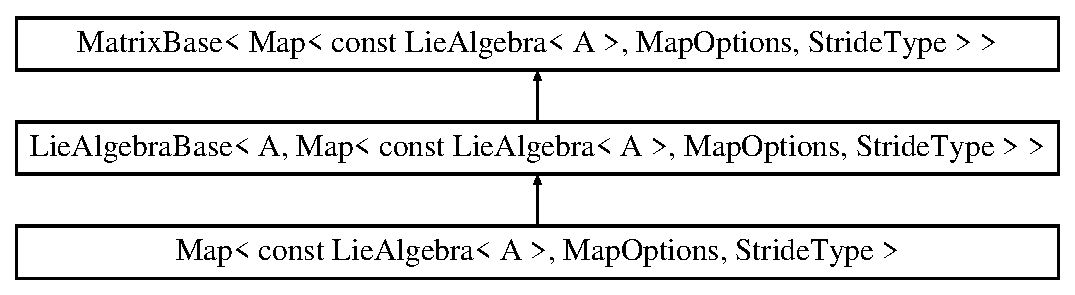
\includegraphics[height=3.000000cm]{class_map_3_01const_01_lie_algebra_3_01_a_01_4_00_01_map_options_00_01_stride_type_01_4}
\end{center}
\end{figure}
\subsection*{Public Types}
\begin{DoxyCompactItemize}
\item 
typedef internal\+::traits$<$ \hyperlink{class_map_3_01const_01_lie_algebra_3_01_a_01_4_00_01_map_options_00_01_stride_type_01_4_a1f3c2cd540feb372191254760225bf1a}{Map}$<$ const \hyperlink{class_lie_algebra}{Lie\+Algebra}$<$ A $>$, Map\+Options, Stride\+Type $>$ $>$\+::\hyperlink{class_map_3_01const_01_lie_algebra_3_01_a_01_4_00_01_map_options_00_01_stride_type_01_4_a3173cdb7a49ee8a41f26cb0891740634}{Coefficients} \hyperlink{class_map_3_01const_01_lie_algebra_3_01_a_01_4_00_01_map_options_00_01_stride_type_01_4_a3173cdb7a49ee8a41f26cb0891740634}{Coefficients}
\end{DoxyCompactItemize}
\subsection*{Public Member Functions}
\begin{DoxyCompactItemize}
\item 
\hyperlink{class_map_3_01const_01_lie_algebra_3_01_a_01_4_00_01_map_options_00_01_stride_type_01_4_a1f3c2cd540feb372191254760225bf1a}{Map} (const A \&a)
\item 
\hyperlink{class_map_3_01const_01_lie_algebra_3_01_a_01_4_00_01_map_options_00_01_stride_type_01_4_a7f5161e409b77fad4e7345c82692c801}{Map} (const Scalar $\ast$data)
\item 
\hyperlink{class_map_3_01const_01_lie_algebra_3_01_a_01_4_00_01_map_options_00_01_stride_type_01_4_aa1bcc912b7d596a67e3fedd49c0a7d75}{Map} (const Map \&m)
\item 
\hyperlink{class_map_3_01const_01_lie_algebra_3_01_a_01_4_00_01_map_options_00_01_stride_type_01_4_a3173cdb7a49ee8a41f26cb0891740634}{Coefficients} \& \hyperlink{class_map_3_01const_01_lie_algebra_3_01_a_01_4_00_01_map_options_00_01_stride_type_01_4_a28ee75aa11e379eea89e0b37ab138d67}{get} ()
\item 
const \hyperlink{class_map_3_01const_01_lie_algebra_3_01_a_01_4_00_01_map_options_00_01_stride_type_01_4_a3173cdb7a49ee8a41f26cb0891740634}{Coefficients} \& \hyperlink{class_map_3_01const_01_lie_algebra_3_01_a_01_4_00_01_map_options_00_01_stride_type_01_4_ac521a54ebd19e30bf20d0a48ea0dce12}{get} () const
\end{DoxyCompactItemize}
\subsection*{Protected Types}
\begin{DoxyCompactItemize}
\item 
typedef \hyperlink{class_lie_algebra_base}{Lie\+Algebra\+Base}$<$ A, \hyperlink{class_map_3_01const_01_lie_algebra_3_01_a_01_4_00_01_map_options_00_01_stride_type_01_4_a1f3c2cd540feb372191254760225bf1a}{Map}$<$ const \hyperlink{class_lie_algebra}{Lie\+Algebra}$<$ A $>$, Map\+Options, Stride\+Type $>$ $>$ \hyperlink{class_map_3_01const_01_lie_algebra_3_01_a_01_4_00_01_map_options_00_01_stride_type_01_4_a166824ba02315d6ccc6f2eda82c268f6}{Base}
\end{DoxyCompactItemize}
\subsection*{Protected Attributes}
\begin{DoxyCompactItemize}
\item 
\hyperlink{class_map_3_01const_01_lie_algebra_3_01_a_01_4_00_01_map_options_00_01_stride_type_01_4_a3173cdb7a49ee8a41f26cb0891740634}{Coefficients} \hyperlink{class_map_3_01const_01_lie_algebra_3_01_a_01_4_00_01_map_options_00_01_stride_type_01_4_a43cc2f5492ebc7467e491b72e61642bb}{m\+\_\+coeffs}
\end{DoxyCompactItemize}


\subsection{Detailed Description}
\subsubsection*{template$<$class A, int Map\+Options, typename Stride\+Type$>$\newline
class Map$<$ const Lie\+Algebra$<$ A $>$, Map\+Options, Stride\+Type $>$}



Definition at line 308 of file Lie\+Algebra.\+h.



\subsection{Member Typedef Documentation}
\hypertarget{class_map_3_01const_01_lie_algebra_3_01_a_01_4_00_01_map_options_00_01_stride_type_01_4_a166824ba02315d6ccc6f2eda82c268f6}{}\label{class_map_3_01const_01_lie_algebra_3_01_a_01_4_00_01_map_options_00_01_stride_type_01_4_a166824ba02315d6ccc6f2eda82c268f6} 
\index{Map$<$ const Lie\+Algebra$<$ A $>$, Map\+Options, Stride\+Type $>$@{Map$<$ const Lie\+Algebra$<$ A $>$, Map\+Options, Stride\+Type $>$}!Base@{Base}}
\index{Base@{Base}!Map$<$ const Lie\+Algebra$<$ A $>$, Map\+Options, Stride\+Type $>$@{Map$<$ const Lie\+Algebra$<$ A $>$, Map\+Options, Stride\+Type $>$}}
\subsubsection{\texorpdfstring{Base}{Base}}
{\footnotesize\ttfamily template$<$class A , int Map\+Options, typename Stride\+Type $>$ \\
typedef \hyperlink{class_lie_algebra_base}{Lie\+Algebra\+Base}$<$A, \hyperlink{class_map_3_01const_01_lie_algebra_3_01_a_01_4_00_01_map_options_00_01_stride_type_01_4_a1f3c2cd540feb372191254760225bf1a}{Map}$<$const \hyperlink{class_lie_algebra}{Lie\+Algebra}$<$A$>$, Map\+Options, Stride\+Type$>$ $>$ \hyperlink{class_map_3_01const_01_lie_algebra_3_01_a_01_4_00_01_map_options_00_01_stride_type_01_4_a1f3c2cd540feb372191254760225bf1a}{Map}$<$ const \hyperlink{class_lie_algebra}{Lie\+Algebra}$<$ A $>$, Map\+Options, Stride\+Type $>$\+::\hyperlink{class_map_3_01const_01_lie_algebra_3_01_a_01_4_00_01_map_options_00_01_stride_type_01_4_a166824ba02315d6ccc6f2eda82c268f6}{Base}\hspace{0.3cm}{\ttfamily [protected]}}

Inherited class 

Definition at line 311 of file Lie\+Algebra.\+h.

\hypertarget{class_map_3_01const_01_lie_algebra_3_01_a_01_4_00_01_map_options_00_01_stride_type_01_4_a3173cdb7a49ee8a41f26cb0891740634}{}\label{class_map_3_01const_01_lie_algebra_3_01_a_01_4_00_01_map_options_00_01_stride_type_01_4_a3173cdb7a49ee8a41f26cb0891740634} 
\index{Map$<$ const Lie\+Algebra$<$ A $>$, Map\+Options, Stride\+Type $>$@{Map$<$ const Lie\+Algebra$<$ A $>$, Map\+Options, Stride\+Type $>$}!Coefficients@{Coefficients}}
\index{Coefficients@{Coefficients}!Map$<$ const Lie\+Algebra$<$ A $>$, Map\+Options, Stride\+Type $>$@{Map$<$ const Lie\+Algebra$<$ A $>$, Map\+Options, Stride\+Type $>$}}
\subsubsection{\texorpdfstring{Coefficients}{Coefficients}}
{\footnotesize\ttfamily template$<$class A , int Map\+Options, typename Stride\+Type $>$ \\
typedef internal\+::traits$<$\hyperlink{class_map_3_01const_01_lie_algebra_3_01_a_01_4_00_01_map_options_00_01_stride_type_01_4_a1f3c2cd540feb372191254760225bf1a}{Map}$<$const \hyperlink{class_lie_algebra}{Lie\+Algebra}$<$A$>$, Map\+Options, Stride\+Type$>$ $>$\+::\hyperlink{class_map_3_01const_01_lie_algebra_3_01_a_01_4_00_01_map_options_00_01_stride_type_01_4_a3173cdb7a49ee8a41f26cb0891740634}{Coefficients} \hyperlink{class_map_3_01const_01_lie_algebra_3_01_a_01_4_00_01_map_options_00_01_stride_type_01_4_a1f3c2cd540feb372191254760225bf1a}{Map}$<$ const \hyperlink{class_lie_algebra}{Lie\+Algebra}$<$ A $>$, Map\+Options, Stride\+Type $>$\+::\hyperlink{class_map_3_01const_01_lie_algebra_3_01_a_01_4_00_01_map_options_00_01_stride_type_01_4_a3173cdb7a49ee8a41f26cb0891740634}{Coefficients}}

The stored coefficients 

Definition at line 317 of file Lie\+Algebra.\+h.



\subsection{Constructor \& Destructor Documentation}
\hypertarget{class_map_3_01const_01_lie_algebra_3_01_a_01_4_00_01_map_options_00_01_stride_type_01_4_a1f3c2cd540feb372191254760225bf1a}{}\label{class_map_3_01const_01_lie_algebra_3_01_a_01_4_00_01_map_options_00_01_stride_type_01_4_a1f3c2cd540feb372191254760225bf1a} 
\index{Map$<$ const Lie\+Algebra$<$ A $>$, Map\+Options, Stride\+Type $>$@{Map$<$ const Lie\+Algebra$<$ A $>$, Map\+Options, Stride\+Type $>$}!Map@{Map}}
\index{Map@{Map}!Map$<$ const Lie\+Algebra$<$ A $>$, Map\+Options, Stride\+Type $>$@{Map$<$ const Lie\+Algebra$<$ A $>$, Map\+Options, Stride\+Type $>$}}
\subsubsection{\texorpdfstring{Map()}{Map()}\hspace{0.1cm}{\footnotesize\ttfamily [1/3]}}
{\footnotesize\ttfamily template$<$class A , int Map\+Options, typename Stride\+Type $>$ \\
Map$<$ const \hyperlink{class_lie_algebra}{Lie\+Algebra}$<$ A $>$, Map\+Options, Stride\+Type $>$\+::Map (\begin{DoxyParamCaption}\item[{const A \&}]{a }\end{DoxyParamCaption})\hspace{0.3cm}{\ttfamily [inline]}}

Maps a class A 

Definition at line 320 of file Lie\+Algebra.\+h.

\hypertarget{class_map_3_01const_01_lie_algebra_3_01_a_01_4_00_01_map_options_00_01_stride_type_01_4_a7f5161e409b77fad4e7345c82692c801}{}\label{class_map_3_01const_01_lie_algebra_3_01_a_01_4_00_01_map_options_00_01_stride_type_01_4_a7f5161e409b77fad4e7345c82692c801} 
\index{Map$<$ const Lie\+Algebra$<$ A $>$, Map\+Options, Stride\+Type $>$@{Map$<$ const Lie\+Algebra$<$ A $>$, Map\+Options, Stride\+Type $>$}!Map@{Map}}
\index{Map@{Map}!Map$<$ const Lie\+Algebra$<$ A $>$, Map\+Options, Stride\+Type $>$@{Map$<$ const Lie\+Algebra$<$ A $>$, Map\+Options, Stride\+Type $>$}}
\subsubsection{\texorpdfstring{Map()}{Map()}\hspace{0.1cm}{\footnotesize\ttfamily [2/3]}}
{\footnotesize\ttfamily template$<$class A , int Map\+Options, typename Stride\+Type $>$ \\
Map$<$ const \hyperlink{class_lie_algebra}{Lie\+Algebra}$<$ A $>$, Map\+Options, Stride\+Type $>$\+::Map (\begin{DoxyParamCaption}\item[{const Scalar $\ast$}]{data }\end{DoxyParamCaption})\hspace{0.3cm}{\ttfamily [inline]}}

Maps an array of scalar 

Definition at line 322 of file Lie\+Algebra.\+h.

\hypertarget{class_map_3_01const_01_lie_algebra_3_01_a_01_4_00_01_map_options_00_01_stride_type_01_4_aa1bcc912b7d596a67e3fedd49c0a7d75}{}\label{class_map_3_01const_01_lie_algebra_3_01_a_01_4_00_01_map_options_00_01_stride_type_01_4_aa1bcc912b7d596a67e3fedd49c0a7d75} 
\index{Map$<$ const Lie\+Algebra$<$ A $>$, Map\+Options, Stride\+Type $>$@{Map$<$ const Lie\+Algebra$<$ A $>$, Map\+Options, Stride\+Type $>$}!Map@{Map}}
\index{Map@{Map}!Map$<$ const Lie\+Algebra$<$ A $>$, Map\+Options, Stride\+Type $>$@{Map$<$ const Lie\+Algebra$<$ A $>$, Map\+Options, Stride\+Type $>$}}
\subsubsection{\texorpdfstring{Map()}{Map()}\hspace{0.1cm}{\footnotesize\ttfamily [3/3]}}
{\footnotesize\ttfamily template$<$class A , int Map\+Options, typename Stride\+Type $>$ \\
Map$<$ const \hyperlink{class_lie_algebra}{Lie\+Algebra}$<$ A $>$, Map\+Options, Stride\+Type $>$\+::Map (\begin{DoxyParamCaption}\item[{const Map$<$ const \hyperlink{class_lie_algebra}{Lie\+Algebra}$<$ A $>$, Map\+Options, Stride\+Type $>$ \&}]{m }\end{DoxyParamCaption})\hspace{0.3cm}{\ttfamily [inline]}}

Maps another Map$<$\+Lie\+Algebra$>$ 

Definition at line 324 of file Lie\+Algebra.\+h.



\subsection{Member Function Documentation}
\hypertarget{class_map_3_01const_01_lie_algebra_3_01_a_01_4_00_01_map_options_00_01_stride_type_01_4_a28ee75aa11e379eea89e0b37ab138d67}{}\label{class_map_3_01const_01_lie_algebra_3_01_a_01_4_00_01_map_options_00_01_stride_type_01_4_a28ee75aa11e379eea89e0b37ab138d67} 
\index{Map$<$ const Lie\+Algebra$<$ A $>$, Map\+Options, Stride\+Type $>$@{Map$<$ const Lie\+Algebra$<$ A $>$, Map\+Options, Stride\+Type $>$}!get@{get}}
\index{get@{get}!Map$<$ const Lie\+Algebra$<$ A $>$, Map\+Options, Stride\+Type $>$@{Map$<$ const Lie\+Algebra$<$ A $>$, Map\+Options, Stride\+Type $>$}}
\subsubsection{\texorpdfstring{get()}{get()}\hspace{0.1cm}{\footnotesize\ttfamily [1/2]}}
{\footnotesize\ttfamily template$<$class A , int Map\+Options, typename Stride\+Type $>$ \\
\hyperlink{class_map_3_01const_01_lie_algebra_3_01_a_01_4_00_01_map_options_00_01_stride_type_01_4_a3173cdb7a49ee8a41f26cb0891740634}{Coefficients}\& \hyperlink{class_map_3_01const_01_lie_algebra_3_01_a_01_4_00_01_map_options_00_01_stride_type_01_4_a1f3c2cd540feb372191254760225bf1a}{Map}$<$ const \hyperlink{class_lie_algebra}{Lie\+Algebra}$<$ A $>$, Map\+Options, Stride\+Type $>$\+::get (\begin{DoxyParamCaption}{ }\end{DoxyParamCaption})\hspace{0.3cm}{\ttfamily [inline]}}

\begin{DoxyReturn}{Returns}
The stored coefficients 
\end{DoxyReturn}


Definition at line 327 of file Lie\+Algebra.\+h.

\hypertarget{class_map_3_01const_01_lie_algebra_3_01_a_01_4_00_01_map_options_00_01_stride_type_01_4_ac521a54ebd19e30bf20d0a48ea0dce12}{}\label{class_map_3_01const_01_lie_algebra_3_01_a_01_4_00_01_map_options_00_01_stride_type_01_4_ac521a54ebd19e30bf20d0a48ea0dce12} 
\index{Map$<$ const Lie\+Algebra$<$ A $>$, Map\+Options, Stride\+Type $>$@{Map$<$ const Lie\+Algebra$<$ A $>$, Map\+Options, Stride\+Type $>$}!get@{get}}
\index{get@{get}!Map$<$ const Lie\+Algebra$<$ A $>$, Map\+Options, Stride\+Type $>$@{Map$<$ const Lie\+Algebra$<$ A $>$, Map\+Options, Stride\+Type $>$}}
\subsubsection{\texorpdfstring{get()}{get()}\hspace{0.1cm}{\footnotesize\ttfamily [2/2]}}
{\footnotesize\ttfamily template$<$class A , int Map\+Options, typename Stride\+Type $>$ \\
const \hyperlink{class_map_3_01const_01_lie_algebra_3_01_a_01_4_00_01_map_options_00_01_stride_type_01_4_a3173cdb7a49ee8a41f26cb0891740634}{Coefficients}\& \hyperlink{class_map_3_01const_01_lie_algebra_3_01_a_01_4_00_01_map_options_00_01_stride_type_01_4_a1f3c2cd540feb372191254760225bf1a}{Map}$<$ const \hyperlink{class_lie_algebra}{Lie\+Algebra}$<$ A $>$, Map\+Options, Stride\+Type $>$\+::get (\begin{DoxyParamCaption}{ }\end{DoxyParamCaption}) const\hspace{0.3cm}{\ttfamily [inline]}}

\begin{DoxyReturn}{Returns}
The read-\/only access to the stored coefficients 
\end{DoxyReturn}


Definition at line 329 of file Lie\+Algebra.\+h.



\subsection{Member Data Documentation}
\hypertarget{class_map_3_01const_01_lie_algebra_3_01_a_01_4_00_01_map_options_00_01_stride_type_01_4_a43cc2f5492ebc7467e491b72e61642bb}{}\label{class_map_3_01const_01_lie_algebra_3_01_a_01_4_00_01_map_options_00_01_stride_type_01_4_a43cc2f5492ebc7467e491b72e61642bb} 
\index{Map$<$ const Lie\+Algebra$<$ A $>$, Map\+Options, Stride\+Type $>$@{Map$<$ const Lie\+Algebra$<$ A $>$, Map\+Options, Stride\+Type $>$}!m\+\_\+coeffs@{m\+\_\+coeffs}}
\index{m\+\_\+coeffs@{m\+\_\+coeffs}!Map$<$ const Lie\+Algebra$<$ A $>$, Map\+Options, Stride\+Type $>$@{Map$<$ const Lie\+Algebra$<$ A $>$, Map\+Options, Stride\+Type $>$}}
\subsubsection{\texorpdfstring{m\+\_\+coeffs}{m\_coeffs}}
{\footnotesize\ttfamily template$<$class A , int Map\+Options, typename Stride\+Type $>$ \\
\hyperlink{class_map_3_01const_01_lie_algebra_3_01_a_01_4_00_01_map_options_00_01_stride_type_01_4_a3173cdb7a49ee8a41f26cb0891740634}{Coefficients} \hyperlink{class_map_3_01const_01_lie_algebra_3_01_a_01_4_00_01_map_options_00_01_stride_type_01_4_a1f3c2cd540feb372191254760225bf1a}{Map}$<$ const \hyperlink{class_lie_algebra}{Lie\+Algebra}$<$ A $>$, Map\+Options, Stride\+Type $>$\+::m\+\_\+coeffs\hspace{0.3cm}{\ttfamily [protected]}}

The wrapped coefficients 

Definition at line 333 of file Lie\+Algebra.\+h.



The documentation for this class was generated from the following file\+:\begin{DoxyCompactItemize}
\item 
/\+Users/\+Ryan/\+Code/codyco-\/superbuild/libraries/\+Eigen\+Lgsm/unsupported/\+Eigen/src/\+Lgsm/\hyperlink{_lie_algebra_8h}{Lie\+Algebra.\+h}\end{DoxyCompactItemize}

\hypertarget{class_map_3_01const_01_lie_algebra_dual_3_01_a_01_4_00_01_map_options_00_01_stride_type_01_4}{}\section{Map$<$ const Lie\+Algebra\+Dual$<$ A $>$, Map\+Options, Stride\+Type $>$ Class Template Reference}
\label{class_map_3_01const_01_lie_algebra_dual_3_01_a_01_4_00_01_map_options_00_01_stride_type_01_4}\index{Map$<$ const Lie\+Algebra\+Dual$<$ A $>$, Map\+Options, Stride\+Type $>$@{Map$<$ const Lie\+Algebra\+Dual$<$ A $>$, Map\+Options, Stride\+Type $>$}}


{\ttfamily \#include $<$Lie\+Algebra.\+h$>$}

Inheritance diagram for Map$<$ const Lie\+Algebra\+Dual$<$ A $>$, Map\+Options, Stride\+Type $>$\+:\begin{figure}[H]
\begin{center}
\leavevmode
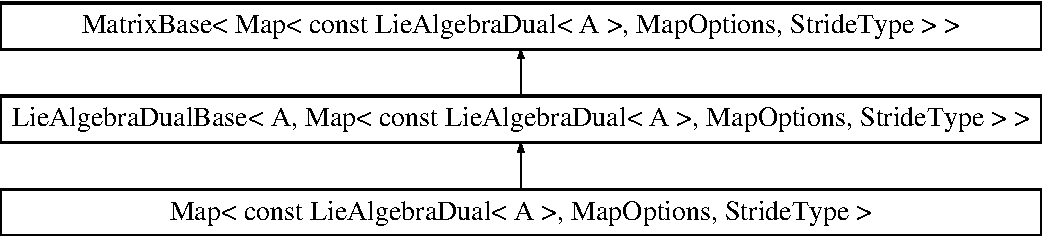
\includegraphics[height=3.000000cm]{class_map_3_01const_01_lie_algebra_dual_3_01_a_01_4_00_01_map_options_00_01_stride_type_01_4}
\end{center}
\end{figure}
\subsection*{Public Types}
\begin{DoxyCompactItemize}
\item 
typedef internal\+::traits$<$ \hyperlink{class_map_3_01const_01_lie_algebra_dual_3_01_a_01_4_00_01_map_options_00_01_stride_type_01_4_a3733e2160ea4f13268b2b3e34b33d7c7}{Map}$<$ const \hyperlink{class_lie_algebra_dual}{Lie\+Algebra\+Dual}$<$ A $>$, Map\+Options, Stride\+Type $>$ $>$\+::\hyperlink{class_map_3_01const_01_lie_algebra_dual_3_01_a_01_4_00_01_map_options_00_01_stride_type_01_4_ae2a817b2902e4bf4f79a40724c8c9341}{Coefficients} \hyperlink{class_map_3_01const_01_lie_algebra_dual_3_01_a_01_4_00_01_map_options_00_01_stride_type_01_4_ae2a817b2902e4bf4f79a40724c8c9341}{Coefficients}
\end{DoxyCompactItemize}
\subsection*{Public Member Functions}
\begin{DoxyCompactItemize}
\item 
\hyperlink{class_map_3_01const_01_lie_algebra_dual_3_01_a_01_4_00_01_map_options_00_01_stride_type_01_4_a3733e2160ea4f13268b2b3e34b33d7c7}{Map} (const A \&a)
\item 
\hyperlink{class_map_3_01const_01_lie_algebra_dual_3_01_a_01_4_00_01_map_options_00_01_stride_type_01_4_ad7a17fb9ef97f7c0dcd412cb97625a88}{Map} (const Scalar $\ast$data)
\item 
\hyperlink{class_map_3_01const_01_lie_algebra_dual_3_01_a_01_4_00_01_map_options_00_01_stride_type_01_4_a8b9ede65605a3251c032c9cb7b4f4c0d}{Map} (const Map \&m)
\item 
\hyperlink{class_map_3_01const_01_lie_algebra_dual_3_01_a_01_4_00_01_map_options_00_01_stride_type_01_4_ae2a817b2902e4bf4f79a40724c8c9341}{Coefficients} \& \hyperlink{class_map_3_01const_01_lie_algebra_dual_3_01_a_01_4_00_01_map_options_00_01_stride_type_01_4_a61b1b1392a7ea136db1a9a7598e76ee0}{get} ()
\item 
const \hyperlink{class_map_3_01const_01_lie_algebra_dual_3_01_a_01_4_00_01_map_options_00_01_stride_type_01_4_ae2a817b2902e4bf4f79a40724c8c9341}{Coefficients} \& \hyperlink{class_map_3_01const_01_lie_algebra_dual_3_01_a_01_4_00_01_map_options_00_01_stride_type_01_4_a13e7ccec6853a91e31f5f209bbb27325}{get} () const
\end{DoxyCompactItemize}
\subsection*{Protected Types}
\begin{DoxyCompactItemize}
\item 
typedef \hyperlink{class_lie_algebra_dual_base}{Lie\+Algebra\+Dual\+Base}$<$ A, \hyperlink{class_map_3_01const_01_lie_algebra_dual_3_01_a_01_4_00_01_map_options_00_01_stride_type_01_4_a3733e2160ea4f13268b2b3e34b33d7c7}{Map}$<$ const \hyperlink{class_lie_algebra_dual}{Lie\+Algebra\+Dual}$<$ A $>$, Map\+Options, Stride\+Type $>$ $>$ \hyperlink{class_map_3_01const_01_lie_algebra_dual_3_01_a_01_4_00_01_map_options_00_01_stride_type_01_4_ae2af81dfcc79fd0a3794e4f13cf9229b}{Base}
\end{DoxyCompactItemize}
\subsection*{Protected Attributes}
\begin{DoxyCompactItemize}
\item 
\hyperlink{class_map_3_01const_01_lie_algebra_dual_3_01_a_01_4_00_01_map_options_00_01_stride_type_01_4_ae2a817b2902e4bf4f79a40724c8c9341}{Coefficients} \hyperlink{class_map_3_01const_01_lie_algebra_dual_3_01_a_01_4_00_01_map_options_00_01_stride_type_01_4_a309ca6ad9fa9ab55a7ec4cc08f136404}{m\+\_\+coeffs}
\end{DoxyCompactItemize}


\subsection{Detailed Description}
\subsubsection*{template$<$class A, int Map\+Options, typename Stride\+Type$>$\newline
class Map$<$ const Lie\+Algebra\+Dual$<$ A $>$, Map\+Options, Stride\+Type $>$}



Definition at line 401 of file Lie\+Algebra.\+h.



\subsection{Member Typedef Documentation}
\hypertarget{class_map_3_01const_01_lie_algebra_dual_3_01_a_01_4_00_01_map_options_00_01_stride_type_01_4_ae2af81dfcc79fd0a3794e4f13cf9229b}{}\label{class_map_3_01const_01_lie_algebra_dual_3_01_a_01_4_00_01_map_options_00_01_stride_type_01_4_ae2af81dfcc79fd0a3794e4f13cf9229b} 
\index{Map$<$ const Lie\+Algebra\+Dual$<$ A $>$, Map\+Options, Stride\+Type $>$@{Map$<$ const Lie\+Algebra\+Dual$<$ A $>$, Map\+Options, Stride\+Type $>$}!Base@{Base}}
\index{Base@{Base}!Map$<$ const Lie\+Algebra\+Dual$<$ A $>$, Map\+Options, Stride\+Type $>$@{Map$<$ const Lie\+Algebra\+Dual$<$ A $>$, Map\+Options, Stride\+Type $>$}}
\subsubsection{\texorpdfstring{Base}{Base}}
{\footnotesize\ttfamily template$<$class A , int Map\+Options, typename Stride\+Type $>$ \\
typedef \hyperlink{class_lie_algebra_dual_base}{Lie\+Algebra\+Dual\+Base}$<$A, \hyperlink{class_map_3_01const_01_lie_algebra_dual_3_01_a_01_4_00_01_map_options_00_01_stride_type_01_4_a3733e2160ea4f13268b2b3e34b33d7c7}{Map}$<$const \hyperlink{class_lie_algebra_dual}{Lie\+Algebra\+Dual}$<$A$>$, Map\+Options, Stride\+Type$>$ $>$ \hyperlink{class_map_3_01const_01_lie_algebra_dual_3_01_a_01_4_00_01_map_options_00_01_stride_type_01_4_a3733e2160ea4f13268b2b3e34b33d7c7}{Map}$<$ const \hyperlink{class_lie_algebra_dual}{Lie\+Algebra\+Dual}$<$ A $>$, Map\+Options, Stride\+Type $>$\+::\hyperlink{class_map_3_01const_01_lie_algebra_dual_3_01_a_01_4_00_01_map_options_00_01_stride_type_01_4_ae2af81dfcc79fd0a3794e4f13cf9229b}{Base}\hspace{0.3cm}{\ttfamily [protected]}}

Inherited class 

Definition at line 404 of file Lie\+Algebra.\+h.

\hypertarget{class_map_3_01const_01_lie_algebra_dual_3_01_a_01_4_00_01_map_options_00_01_stride_type_01_4_ae2a817b2902e4bf4f79a40724c8c9341}{}\label{class_map_3_01const_01_lie_algebra_dual_3_01_a_01_4_00_01_map_options_00_01_stride_type_01_4_ae2a817b2902e4bf4f79a40724c8c9341} 
\index{Map$<$ const Lie\+Algebra\+Dual$<$ A $>$, Map\+Options, Stride\+Type $>$@{Map$<$ const Lie\+Algebra\+Dual$<$ A $>$, Map\+Options, Stride\+Type $>$}!Coefficients@{Coefficients}}
\index{Coefficients@{Coefficients}!Map$<$ const Lie\+Algebra\+Dual$<$ A $>$, Map\+Options, Stride\+Type $>$@{Map$<$ const Lie\+Algebra\+Dual$<$ A $>$, Map\+Options, Stride\+Type $>$}}
\subsubsection{\texorpdfstring{Coefficients}{Coefficients}}
{\footnotesize\ttfamily template$<$class A , int Map\+Options, typename Stride\+Type $>$ \\
typedef internal\+::traits$<$\hyperlink{class_map_3_01const_01_lie_algebra_dual_3_01_a_01_4_00_01_map_options_00_01_stride_type_01_4_a3733e2160ea4f13268b2b3e34b33d7c7}{Map}$<$const \hyperlink{class_lie_algebra_dual}{Lie\+Algebra\+Dual}$<$A$>$, Map\+Options, Stride\+Type$>$ $>$\+::\hyperlink{class_map_3_01const_01_lie_algebra_dual_3_01_a_01_4_00_01_map_options_00_01_stride_type_01_4_ae2a817b2902e4bf4f79a40724c8c9341}{Coefficients} \hyperlink{class_map_3_01const_01_lie_algebra_dual_3_01_a_01_4_00_01_map_options_00_01_stride_type_01_4_a3733e2160ea4f13268b2b3e34b33d7c7}{Map}$<$ const \hyperlink{class_lie_algebra_dual}{Lie\+Algebra\+Dual}$<$ A $>$, Map\+Options, Stride\+Type $>$\+::\hyperlink{class_map_3_01const_01_lie_algebra_dual_3_01_a_01_4_00_01_map_options_00_01_stride_type_01_4_ae2a817b2902e4bf4f79a40724c8c9341}{Coefficients}}

The stored coefficients 

Definition at line 410 of file Lie\+Algebra.\+h.



\subsection{Constructor \& Destructor Documentation}
\hypertarget{class_map_3_01const_01_lie_algebra_dual_3_01_a_01_4_00_01_map_options_00_01_stride_type_01_4_a3733e2160ea4f13268b2b3e34b33d7c7}{}\label{class_map_3_01const_01_lie_algebra_dual_3_01_a_01_4_00_01_map_options_00_01_stride_type_01_4_a3733e2160ea4f13268b2b3e34b33d7c7} 
\index{Map$<$ const Lie\+Algebra\+Dual$<$ A $>$, Map\+Options, Stride\+Type $>$@{Map$<$ const Lie\+Algebra\+Dual$<$ A $>$, Map\+Options, Stride\+Type $>$}!Map@{Map}}
\index{Map@{Map}!Map$<$ const Lie\+Algebra\+Dual$<$ A $>$, Map\+Options, Stride\+Type $>$@{Map$<$ const Lie\+Algebra\+Dual$<$ A $>$, Map\+Options, Stride\+Type $>$}}
\subsubsection{\texorpdfstring{Map()}{Map()}\hspace{0.1cm}{\footnotesize\ttfamily [1/3]}}
{\footnotesize\ttfamily template$<$class A , int Map\+Options, typename Stride\+Type $>$ \\
Map$<$ const \hyperlink{class_lie_algebra_dual}{Lie\+Algebra\+Dual}$<$ A $>$, Map\+Options, Stride\+Type $>$\+::Map (\begin{DoxyParamCaption}\item[{const A \&}]{a }\end{DoxyParamCaption})\hspace{0.3cm}{\ttfamily [inline]}}

Maps a class A 

Definition at line 413 of file Lie\+Algebra.\+h.

\hypertarget{class_map_3_01const_01_lie_algebra_dual_3_01_a_01_4_00_01_map_options_00_01_stride_type_01_4_ad7a17fb9ef97f7c0dcd412cb97625a88}{}\label{class_map_3_01const_01_lie_algebra_dual_3_01_a_01_4_00_01_map_options_00_01_stride_type_01_4_ad7a17fb9ef97f7c0dcd412cb97625a88} 
\index{Map$<$ const Lie\+Algebra\+Dual$<$ A $>$, Map\+Options, Stride\+Type $>$@{Map$<$ const Lie\+Algebra\+Dual$<$ A $>$, Map\+Options, Stride\+Type $>$}!Map@{Map}}
\index{Map@{Map}!Map$<$ const Lie\+Algebra\+Dual$<$ A $>$, Map\+Options, Stride\+Type $>$@{Map$<$ const Lie\+Algebra\+Dual$<$ A $>$, Map\+Options, Stride\+Type $>$}}
\subsubsection{\texorpdfstring{Map()}{Map()}\hspace{0.1cm}{\footnotesize\ttfamily [2/3]}}
{\footnotesize\ttfamily template$<$class A , int Map\+Options, typename Stride\+Type $>$ \\
Map$<$ const \hyperlink{class_lie_algebra_dual}{Lie\+Algebra\+Dual}$<$ A $>$, Map\+Options, Stride\+Type $>$\+::Map (\begin{DoxyParamCaption}\item[{const Scalar $\ast$}]{data }\end{DoxyParamCaption})\hspace{0.3cm}{\ttfamily [inline]}}

Maps an array of scalar 

Definition at line 415 of file Lie\+Algebra.\+h.

\hypertarget{class_map_3_01const_01_lie_algebra_dual_3_01_a_01_4_00_01_map_options_00_01_stride_type_01_4_a8b9ede65605a3251c032c9cb7b4f4c0d}{}\label{class_map_3_01const_01_lie_algebra_dual_3_01_a_01_4_00_01_map_options_00_01_stride_type_01_4_a8b9ede65605a3251c032c9cb7b4f4c0d} 
\index{Map$<$ const Lie\+Algebra\+Dual$<$ A $>$, Map\+Options, Stride\+Type $>$@{Map$<$ const Lie\+Algebra\+Dual$<$ A $>$, Map\+Options, Stride\+Type $>$}!Map@{Map}}
\index{Map@{Map}!Map$<$ const Lie\+Algebra\+Dual$<$ A $>$, Map\+Options, Stride\+Type $>$@{Map$<$ const Lie\+Algebra\+Dual$<$ A $>$, Map\+Options, Stride\+Type $>$}}
\subsubsection{\texorpdfstring{Map()}{Map()}\hspace{0.1cm}{\footnotesize\ttfamily [3/3]}}
{\footnotesize\ttfamily template$<$class A , int Map\+Options, typename Stride\+Type $>$ \\
Map$<$ const \hyperlink{class_lie_algebra_dual}{Lie\+Algebra\+Dual}$<$ A $>$, Map\+Options, Stride\+Type $>$\+::Map (\begin{DoxyParamCaption}\item[{const Map$<$ const \hyperlink{class_lie_algebra_dual}{Lie\+Algebra\+Dual}$<$ A $>$, Map\+Options, Stride\+Type $>$ \&}]{m }\end{DoxyParamCaption})\hspace{0.3cm}{\ttfamily [inline]}}

Maps another Map$<$\+Lie\+Algebra$>$ 

Definition at line 417 of file Lie\+Algebra.\+h.



\subsection{Member Function Documentation}
\hypertarget{class_map_3_01const_01_lie_algebra_dual_3_01_a_01_4_00_01_map_options_00_01_stride_type_01_4_a61b1b1392a7ea136db1a9a7598e76ee0}{}\label{class_map_3_01const_01_lie_algebra_dual_3_01_a_01_4_00_01_map_options_00_01_stride_type_01_4_a61b1b1392a7ea136db1a9a7598e76ee0} 
\index{Map$<$ const Lie\+Algebra\+Dual$<$ A $>$, Map\+Options, Stride\+Type $>$@{Map$<$ const Lie\+Algebra\+Dual$<$ A $>$, Map\+Options, Stride\+Type $>$}!get@{get}}
\index{get@{get}!Map$<$ const Lie\+Algebra\+Dual$<$ A $>$, Map\+Options, Stride\+Type $>$@{Map$<$ const Lie\+Algebra\+Dual$<$ A $>$, Map\+Options, Stride\+Type $>$}}
\subsubsection{\texorpdfstring{get()}{get()}\hspace{0.1cm}{\footnotesize\ttfamily [1/2]}}
{\footnotesize\ttfamily template$<$class A , int Map\+Options, typename Stride\+Type $>$ \\
\hyperlink{class_map_3_01const_01_lie_algebra_dual_3_01_a_01_4_00_01_map_options_00_01_stride_type_01_4_ae2a817b2902e4bf4f79a40724c8c9341}{Coefficients}\& \hyperlink{class_map_3_01const_01_lie_algebra_dual_3_01_a_01_4_00_01_map_options_00_01_stride_type_01_4_a3733e2160ea4f13268b2b3e34b33d7c7}{Map}$<$ const \hyperlink{class_lie_algebra_dual}{Lie\+Algebra\+Dual}$<$ A $>$, Map\+Options, Stride\+Type $>$\+::get (\begin{DoxyParamCaption}{ }\end{DoxyParamCaption})\hspace{0.3cm}{\ttfamily [inline]}}

\begin{DoxyReturn}{Returns}
The stored coefficients 
\end{DoxyReturn}


Definition at line 420 of file Lie\+Algebra.\+h.

\hypertarget{class_map_3_01const_01_lie_algebra_dual_3_01_a_01_4_00_01_map_options_00_01_stride_type_01_4_a13e7ccec6853a91e31f5f209bbb27325}{}\label{class_map_3_01const_01_lie_algebra_dual_3_01_a_01_4_00_01_map_options_00_01_stride_type_01_4_a13e7ccec6853a91e31f5f209bbb27325} 
\index{Map$<$ const Lie\+Algebra\+Dual$<$ A $>$, Map\+Options, Stride\+Type $>$@{Map$<$ const Lie\+Algebra\+Dual$<$ A $>$, Map\+Options, Stride\+Type $>$}!get@{get}}
\index{get@{get}!Map$<$ const Lie\+Algebra\+Dual$<$ A $>$, Map\+Options, Stride\+Type $>$@{Map$<$ const Lie\+Algebra\+Dual$<$ A $>$, Map\+Options, Stride\+Type $>$}}
\subsubsection{\texorpdfstring{get()}{get()}\hspace{0.1cm}{\footnotesize\ttfamily [2/2]}}
{\footnotesize\ttfamily template$<$class A , int Map\+Options, typename Stride\+Type $>$ \\
const \hyperlink{class_map_3_01const_01_lie_algebra_dual_3_01_a_01_4_00_01_map_options_00_01_stride_type_01_4_ae2a817b2902e4bf4f79a40724c8c9341}{Coefficients}\& \hyperlink{class_map_3_01const_01_lie_algebra_dual_3_01_a_01_4_00_01_map_options_00_01_stride_type_01_4_a3733e2160ea4f13268b2b3e34b33d7c7}{Map}$<$ const \hyperlink{class_lie_algebra_dual}{Lie\+Algebra\+Dual}$<$ A $>$, Map\+Options, Stride\+Type $>$\+::get (\begin{DoxyParamCaption}{ }\end{DoxyParamCaption}) const\hspace{0.3cm}{\ttfamily [inline]}}

\begin{DoxyReturn}{Returns}
The read-\/only access to the stored coefficients 
\end{DoxyReturn}


Definition at line 422 of file Lie\+Algebra.\+h.



\subsection{Member Data Documentation}
\hypertarget{class_map_3_01const_01_lie_algebra_dual_3_01_a_01_4_00_01_map_options_00_01_stride_type_01_4_a309ca6ad9fa9ab55a7ec4cc08f136404}{}\label{class_map_3_01const_01_lie_algebra_dual_3_01_a_01_4_00_01_map_options_00_01_stride_type_01_4_a309ca6ad9fa9ab55a7ec4cc08f136404} 
\index{Map$<$ const Lie\+Algebra\+Dual$<$ A $>$, Map\+Options, Stride\+Type $>$@{Map$<$ const Lie\+Algebra\+Dual$<$ A $>$, Map\+Options, Stride\+Type $>$}!m\+\_\+coeffs@{m\+\_\+coeffs}}
\index{m\+\_\+coeffs@{m\+\_\+coeffs}!Map$<$ const Lie\+Algebra\+Dual$<$ A $>$, Map\+Options, Stride\+Type $>$@{Map$<$ const Lie\+Algebra\+Dual$<$ A $>$, Map\+Options, Stride\+Type $>$}}
\subsubsection{\texorpdfstring{m\+\_\+coeffs}{m\_coeffs}}
{\footnotesize\ttfamily template$<$class A , int Map\+Options, typename Stride\+Type $>$ \\
\hyperlink{class_map_3_01const_01_lie_algebra_dual_3_01_a_01_4_00_01_map_options_00_01_stride_type_01_4_ae2a817b2902e4bf4f79a40724c8c9341}{Coefficients} \hyperlink{class_map_3_01const_01_lie_algebra_dual_3_01_a_01_4_00_01_map_options_00_01_stride_type_01_4_a3733e2160ea4f13268b2b3e34b33d7c7}{Map}$<$ const \hyperlink{class_lie_algebra_dual}{Lie\+Algebra\+Dual}$<$ A $>$, Map\+Options, Stride\+Type $>$\+::m\+\_\+coeffs\hspace{0.3cm}{\ttfamily [protected]}}

The wrapped coefficients 

Definition at line 426 of file Lie\+Algebra.\+h.



The documentation for this class was generated from the following file\+:\begin{DoxyCompactItemize}
\item 
/\+Users/\+Ryan/\+Code/codyco-\/superbuild/libraries/\+Eigen\+Lgsm/unsupported/\+Eigen/src/\+Lgsm/\hyperlink{_lie_algebra_8h}{Lie\+Algebra.\+h}\end{DoxyCompactItemize}

\hypertarget{class_map_3_01const_01_lie_group_3_01_g_01_4_00_01_map_options_00_01_stride_type_01_4}{}\section{Map$<$ const Lie\+Group$<$ G $>$, Map\+Options, Stride\+Type $>$ Class Template Reference}
\label{class_map_3_01const_01_lie_group_3_01_g_01_4_00_01_map_options_00_01_stride_type_01_4}\index{Map$<$ const Lie\+Group$<$ G $>$, Map\+Options, Stride\+Type $>$@{Map$<$ const Lie\+Group$<$ G $>$, Map\+Options, Stride\+Type $>$}}


{\ttfamily \#include $<$Lie\+Group.\+h$>$}

Inheritance diagram for Map$<$ const Lie\+Group$<$ G $>$, Map\+Options, Stride\+Type $>$\+:\begin{figure}[H]
\begin{center}
\leavevmode
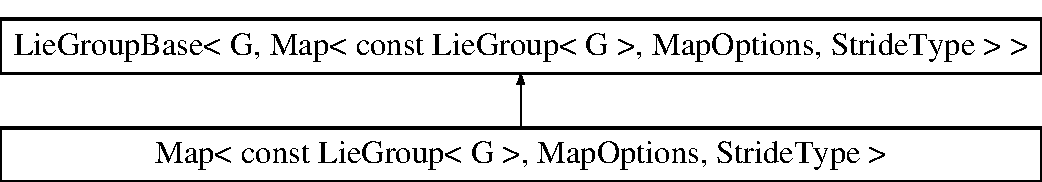
\includegraphics[height=2.000000cm]{class_map_3_01const_01_lie_group_3_01_g_01_4_00_01_map_options_00_01_stride_type_01_4}
\end{center}
\end{figure}
\subsection*{Public Types}
\begin{DoxyCompactItemize}
\item 
typedef internal\+::traits$<$ \hyperlink{class_map_3_01const_01_lie_group_3_01_g_01_4_00_01_map_options_00_01_stride_type_01_4_a95174b5f6c93ceefa0fbc6ef6fdf65f7}{Map}$<$ const \hyperlink{class_lie_group}{Lie\+Group}$<$ G $>$, Map\+Options, Stride\+Type $>$ $>$\+::\hyperlink{class_map_3_01const_01_lie_group_3_01_g_01_4_00_01_map_options_00_01_stride_type_01_4_a006635f5fe4155200809ee347f61b9a6}{Scalar} \hyperlink{class_map_3_01const_01_lie_group_3_01_g_01_4_00_01_map_options_00_01_stride_type_01_4_a006635f5fe4155200809ee347f61b9a6}{Scalar}
\item 
typedef internal\+::traits$<$ \hyperlink{class_map_3_01const_01_lie_group_3_01_g_01_4_00_01_map_options_00_01_stride_type_01_4_a95174b5f6c93ceefa0fbc6ef6fdf65f7}{Map}$<$ const \hyperlink{class_lie_group}{Lie\+Group}$<$ G $>$, Map\+Options, Stride\+Type $>$ $>$\+::\hyperlink{class_map_3_01const_01_lie_group_3_01_g_01_4_00_01_map_options_00_01_stride_type_01_4_a670729f8e6ab1131541ef46da7d09274}{Coefficients} \hyperlink{class_map_3_01const_01_lie_group_3_01_g_01_4_00_01_map_options_00_01_stride_type_01_4_a670729f8e6ab1131541ef46da7d09274}{Coefficients}
\end{DoxyCompactItemize}
\subsection*{Public Member Functions}
\begin{DoxyCompactItemize}
\item 
\hyperlink{class_map_3_01const_01_lie_group_3_01_g_01_4_00_01_map_options_00_01_stride_type_01_4_a95174b5f6c93ceefa0fbc6ef6fdf65f7}{Map} (const G \&g)
\item 
{\footnotesize template$<$int \+\_\+\+Rows, int \+\_\+\+Cols, int \+\_\+\+Options, int \+\_\+\+Max\+Rows, int \+\_\+\+Max\+Cols$>$ }\\\hyperlink{class_map_3_01const_01_lie_group_3_01_g_01_4_00_01_map_options_00_01_stride_type_01_4_a5e4ba9f00368b29fdb6d8948d2f56c5b}{Map} (Array$<$ \hyperlink{class_map_3_01const_01_lie_group_3_01_g_01_4_00_01_map_options_00_01_stride_type_01_4_a006635f5fe4155200809ee347f61b9a6}{Scalar}, \+\_\+\+Rows, \+\_\+\+Cols, \+\_\+\+Options, \+\_\+\+Max\+Rows, \+\_\+\+Max\+Cols $>$ \&g)
\item 
\hyperlink{class_map_3_01const_01_lie_group_3_01_g_01_4_00_01_map_options_00_01_stride_type_01_4_a47888b3035c416eb5fadeb6d8e4026a2}{Map} (const \hyperlink{class_map_3_01const_01_lie_group_3_01_g_01_4_00_01_map_options_00_01_stride_type_01_4_a006635f5fe4155200809ee347f61b9a6}{Scalar} $\ast$data)
\item 
\hyperlink{class_map_3_01const_01_lie_group_3_01_g_01_4_00_01_map_options_00_01_stride_type_01_4_a0aadabe587f3f92d994d4a0247bc0f72}{Map} (const Map \&m)
\item 
\hyperlink{class_map_3_01const_01_lie_group_3_01_g_01_4_00_01_map_options_00_01_stride_type_01_4_a670729f8e6ab1131541ef46da7d09274}{Coefficients} \& \hyperlink{class_map_3_01const_01_lie_group_3_01_g_01_4_00_01_map_options_00_01_stride_type_01_4_ab48c4783f796ef888b9c9dc3a78fb35a}{get} ()
\item 
const \hyperlink{class_map_3_01const_01_lie_group_3_01_g_01_4_00_01_map_options_00_01_stride_type_01_4_a670729f8e6ab1131541ef46da7d09274}{Coefficients} \& \hyperlink{class_map_3_01const_01_lie_group_3_01_g_01_4_00_01_map_options_00_01_stride_type_01_4_aa9bd0922b1e369ac08f43921453d330c}{get} () const
\end{DoxyCompactItemize}
\subsection*{Protected Types}
\begin{DoxyCompactItemize}
\item 
typedef \hyperlink{class_lie_group_base}{Lie\+Group\+Base}$<$ G, \hyperlink{class_map_3_01const_01_lie_group_3_01_g_01_4_00_01_map_options_00_01_stride_type_01_4_a95174b5f6c93ceefa0fbc6ef6fdf65f7}{Map}$<$ const \hyperlink{class_lie_group}{Lie\+Group}$<$ G $>$, Map\+Options, Stride\+Type $>$ $>$ \hyperlink{class_map_3_01const_01_lie_group_3_01_g_01_4_00_01_map_options_00_01_stride_type_01_4_ae8127dbfe0e6b6b515d319062f495883}{Base}
\end{DoxyCompactItemize}
\subsection*{Protected Attributes}
\begin{DoxyCompactItemize}
\item 
\hyperlink{class_map_3_01const_01_lie_group_3_01_g_01_4_00_01_map_options_00_01_stride_type_01_4_a670729f8e6ab1131541ef46da7d09274}{Coefficients} \hyperlink{class_map_3_01const_01_lie_group_3_01_g_01_4_00_01_map_options_00_01_stride_type_01_4_a3dcc1fda9634e88e41a81209f408a8e8}{m\+\_\+coeffs}
\end{DoxyCompactItemize}
\subsection*{Additional Inherited Members}


\subsection{Detailed Description}
\subsubsection*{template$<$class G, int Map\+Options, typename Stride\+Type$>$\newline
class Map$<$ const Lie\+Group$<$ G $>$, Map\+Options, Stride\+Type $>$}



Definition at line 210 of file Lie\+Group.\+h.



\subsection{Member Typedef Documentation}
\hypertarget{class_map_3_01const_01_lie_group_3_01_g_01_4_00_01_map_options_00_01_stride_type_01_4_ae8127dbfe0e6b6b515d319062f495883}{}\label{class_map_3_01const_01_lie_group_3_01_g_01_4_00_01_map_options_00_01_stride_type_01_4_ae8127dbfe0e6b6b515d319062f495883} 
\index{Map$<$ const Lie\+Group$<$ G $>$, Map\+Options, Stride\+Type $>$@{Map$<$ const Lie\+Group$<$ G $>$, Map\+Options, Stride\+Type $>$}!Base@{Base}}
\index{Base@{Base}!Map$<$ const Lie\+Group$<$ G $>$, Map\+Options, Stride\+Type $>$@{Map$<$ const Lie\+Group$<$ G $>$, Map\+Options, Stride\+Type $>$}}
\subsubsection{\texorpdfstring{Base}{Base}}
{\footnotesize\ttfamily template$<$class G , int Map\+Options, typename Stride\+Type $>$ \\
typedef \hyperlink{class_lie_group_base}{Lie\+Group\+Base}$<$G, \hyperlink{class_map_3_01const_01_lie_group_3_01_g_01_4_00_01_map_options_00_01_stride_type_01_4_a95174b5f6c93ceefa0fbc6ef6fdf65f7}{Map}$<$const \hyperlink{class_lie_group}{Lie\+Group}$<$G$>$, Map\+Options, Stride\+Type $>$ $>$ \hyperlink{class_map_3_01const_01_lie_group_3_01_g_01_4_00_01_map_options_00_01_stride_type_01_4_a95174b5f6c93ceefa0fbc6ef6fdf65f7}{Map}$<$ const \hyperlink{class_lie_group}{Lie\+Group}$<$ G $>$, Map\+Options, Stride\+Type $>$\+::\hyperlink{class_map_3_01const_01_lie_group_3_01_g_01_4_00_01_map_options_00_01_stride_type_01_4_ae8127dbfe0e6b6b515d319062f495883}{Base}\hspace{0.3cm}{\ttfamily [protected]}}

Inherited class 

Definition at line 213 of file Lie\+Group.\+h.

\hypertarget{class_map_3_01const_01_lie_group_3_01_g_01_4_00_01_map_options_00_01_stride_type_01_4_a670729f8e6ab1131541ef46da7d09274}{}\label{class_map_3_01const_01_lie_group_3_01_g_01_4_00_01_map_options_00_01_stride_type_01_4_a670729f8e6ab1131541ef46da7d09274} 
\index{Map$<$ const Lie\+Group$<$ G $>$, Map\+Options, Stride\+Type $>$@{Map$<$ const Lie\+Group$<$ G $>$, Map\+Options, Stride\+Type $>$}!Coefficients@{Coefficients}}
\index{Coefficients@{Coefficients}!Map$<$ const Lie\+Group$<$ G $>$, Map\+Options, Stride\+Type $>$@{Map$<$ const Lie\+Group$<$ G $>$, Map\+Options, Stride\+Type $>$}}
\subsubsection{\texorpdfstring{Coefficients}{Coefficients}}
{\footnotesize\ttfamily template$<$class G , int Map\+Options, typename Stride\+Type $>$ \\
typedef internal\+::traits$<$\hyperlink{class_map_3_01const_01_lie_group_3_01_g_01_4_00_01_map_options_00_01_stride_type_01_4_a95174b5f6c93ceefa0fbc6ef6fdf65f7}{Map}$<$const \hyperlink{class_lie_group}{Lie\+Group}$<$G$>$, Map\+Options, Stride\+Type$>$ $>$\+::\hyperlink{class_map_3_01const_01_lie_group_3_01_g_01_4_00_01_map_options_00_01_stride_type_01_4_a670729f8e6ab1131541ef46da7d09274}{Coefficients} \hyperlink{class_map_3_01const_01_lie_group_3_01_g_01_4_00_01_map_options_00_01_stride_type_01_4_a95174b5f6c93ceefa0fbc6ef6fdf65f7}{Map}$<$ const \hyperlink{class_lie_group}{Lie\+Group}$<$ G $>$, Map\+Options, Stride\+Type $>$\+::\hyperlink{class_map_3_01const_01_lie_group_3_01_g_01_4_00_01_map_options_00_01_stride_type_01_4_a670729f8e6ab1131541ef46da7d09274}{Coefficients}}

The stored coefficients 

Definition at line 220 of file Lie\+Group.\+h.

\hypertarget{class_map_3_01const_01_lie_group_3_01_g_01_4_00_01_map_options_00_01_stride_type_01_4_a006635f5fe4155200809ee347f61b9a6}{}\label{class_map_3_01const_01_lie_group_3_01_g_01_4_00_01_map_options_00_01_stride_type_01_4_a006635f5fe4155200809ee347f61b9a6} 
\index{Map$<$ const Lie\+Group$<$ G $>$, Map\+Options, Stride\+Type $>$@{Map$<$ const Lie\+Group$<$ G $>$, Map\+Options, Stride\+Type $>$}!Scalar@{Scalar}}
\index{Scalar@{Scalar}!Map$<$ const Lie\+Group$<$ G $>$, Map\+Options, Stride\+Type $>$@{Map$<$ const Lie\+Group$<$ G $>$, Map\+Options, Stride\+Type $>$}}
\subsubsection{\texorpdfstring{Scalar}{Scalar}}
{\footnotesize\ttfamily template$<$class G , int Map\+Options, typename Stride\+Type $>$ \\
typedef internal\+::traits$<$\hyperlink{class_map_3_01const_01_lie_group_3_01_g_01_4_00_01_map_options_00_01_stride_type_01_4_a95174b5f6c93ceefa0fbc6ef6fdf65f7}{Map}$<$const \hyperlink{class_lie_group}{Lie\+Group}$<$G$>$, Map\+Options, Stride\+Type$>$ $>$\+::\hyperlink{class_map_3_01const_01_lie_group_3_01_g_01_4_00_01_map_options_00_01_stride_type_01_4_a006635f5fe4155200809ee347f61b9a6}{Scalar} \hyperlink{class_map_3_01const_01_lie_group_3_01_g_01_4_00_01_map_options_00_01_stride_type_01_4_a95174b5f6c93ceefa0fbc6ef6fdf65f7}{Map}$<$ const \hyperlink{class_lie_group}{Lie\+Group}$<$ G $>$, Map\+Options, Stride\+Type $>$\+::\hyperlink{class_map_3_01const_01_lie_group_3_01_g_01_4_00_01_map_options_00_01_stride_type_01_4_a006635f5fe4155200809ee347f61b9a6}{Scalar}}

Coefficients type 

Definition at line 218 of file Lie\+Group.\+h.



\subsection{Constructor \& Destructor Documentation}
\hypertarget{class_map_3_01const_01_lie_group_3_01_g_01_4_00_01_map_options_00_01_stride_type_01_4_a95174b5f6c93ceefa0fbc6ef6fdf65f7}{}\label{class_map_3_01const_01_lie_group_3_01_g_01_4_00_01_map_options_00_01_stride_type_01_4_a95174b5f6c93ceefa0fbc6ef6fdf65f7} 
\index{Map$<$ const Lie\+Group$<$ G $>$, Map\+Options, Stride\+Type $>$@{Map$<$ const Lie\+Group$<$ G $>$, Map\+Options, Stride\+Type $>$}!Map@{Map}}
\index{Map@{Map}!Map$<$ const Lie\+Group$<$ G $>$, Map\+Options, Stride\+Type $>$@{Map$<$ const Lie\+Group$<$ G $>$, Map\+Options, Stride\+Type $>$}}
\subsubsection{\texorpdfstring{Map()}{Map()}\hspace{0.1cm}{\footnotesize\ttfamily [1/4]}}
{\footnotesize\ttfamily template$<$class G , int Map\+Options, typename Stride\+Type $>$ \\
Map$<$ const \hyperlink{class_lie_group}{Lie\+Group}$<$ G $>$, Map\+Options, Stride\+Type $>$\+::Map (\begin{DoxyParamCaption}\item[{const G \&}]{g }\end{DoxyParamCaption})\hspace{0.3cm}{\ttfamily [inline]}}

Maps a class G 

Definition at line 223 of file Lie\+Group.\+h.

\hypertarget{class_map_3_01const_01_lie_group_3_01_g_01_4_00_01_map_options_00_01_stride_type_01_4_a5e4ba9f00368b29fdb6d8948d2f56c5b}{}\label{class_map_3_01const_01_lie_group_3_01_g_01_4_00_01_map_options_00_01_stride_type_01_4_a5e4ba9f00368b29fdb6d8948d2f56c5b} 
\index{Map$<$ const Lie\+Group$<$ G $>$, Map\+Options, Stride\+Type $>$@{Map$<$ const Lie\+Group$<$ G $>$, Map\+Options, Stride\+Type $>$}!Map@{Map}}
\index{Map@{Map}!Map$<$ const Lie\+Group$<$ G $>$, Map\+Options, Stride\+Type $>$@{Map$<$ const Lie\+Group$<$ G $>$, Map\+Options, Stride\+Type $>$}}
\subsubsection{\texorpdfstring{Map()}{Map()}\hspace{0.1cm}{\footnotesize\ttfamily [2/4]}}
{\footnotesize\ttfamily template$<$class G , int Map\+Options, typename Stride\+Type $>$ \\
template$<$int \+\_\+\+Rows, int \+\_\+\+Cols, int \+\_\+\+Options, int \+\_\+\+Max\+Rows, int \+\_\+\+Max\+Cols$>$ \\
Map$<$ const \hyperlink{class_lie_group}{Lie\+Group}$<$ G $>$, Map\+Options, Stride\+Type $>$\+::Map (\begin{DoxyParamCaption}\item[{Array$<$ \hyperlink{class_map_3_01const_01_lie_group_3_01_g_01_4_00_01_map_options_00_01_stride_type_01_4_a006635f5fe4155200809ee347f61b9a6}{Scalar}, \+\_\+\+Rows, \+\_\+\+Cols, \+\_\+\+Options, \+\_\+\+Max\+Rows, \+\_\+\+Max\+Cols $>$ \&}]{g }\end{DoxyParamCaption})\hspace{0.3cm}{\ttfamily [inline]}}

Maps an Array 

Definition at line 226 of file Lie\+Group.\+h.

\hypertarget{class_map_3_01const_01_lie_group_3_01_g_01_4_00_01_map_options_00_01_stride_type_01_4_a47888b3035c416eb5fadeb6d8e4026a2}{}\label{class_map_3_01const_01_lie_group_3_01_g_01_4_00_01_map_options_00_01_stride_type_01_4_a47888b3035c416eb5fadeb6d8e4026a2} 
\index{Map$<$ const Lie\+Group$<$ G $>$, Map\+Options, Stride\+Type $>$@{Map$<$ const Lie\+Group$<$ G $>$, Map\+Options, Stride\+Type $>$}!Map@{Map}}
\index{Map@{Map}!Map$<$ const Lie\+Group$<$ G $>$, Map\+Options, Stride\+Type $>$@{Map$<$ const Lie\+Group$<$ G $>$, Map\+Options, Stride\+Type $>$}}
\subsubsection{\texorpdfstring{Map()}{Map()}\hspace{0.1cm}{\footnotesize\ttfamily [3/4]}}
{\footnotesize\ttfamily template$<$class G , int Map\+Options, typename Stride\+Type $>$ \\
Map$<$ const \hyperlink{class_lie_group}{Lie\+Group}$<$ G $>$, Map\+Options, Stride\+Type $>$\+::Map (\begin{DoxyParamCaption}\item[{const \hyperlink{class_map_3_01const_01_lie_group_3_01_g_01_4_00_01_map_options_00_01_stride_type_01_4_a006635f5fe4155200809ee347f61b9a6}{Scalar} $\ast$}]{data }\end{DoxyParamCaption})\hspace{0.3cm}{\ttfamily [inline]}}

Maps an array of scalar 

Definition at line 228 of file Lie\+Group.\+h.

\hypertarget{class_map_3_01const_01_lie_group_3_01_g_01_4_00_01_map_options_00_01_stride_type_01_4_a0aadabe587f3f92d994d4a0247bc0f72}{}\label{class_map_3_01const_01_lie_group_3_01_g_01_4_00_01_map_options_00_01_stride_type_01_4_a0aadabe587f3f92d994d4a0247bc0f72} 
\index{Map$<$ const Lie\+Group$<$ G $>$, Map\+Options, Stride\+Type $>$@{Map$<$ const Lie\+Group$<$ G $>$, Map\+Options, Stride\+Type $>$}!Map@{Map}}
\index{Map@{Map}!Map$<$ const Lie\+Group$<$ G $>$, Map\+Options, Stride\+Type $>$@{Map$<$ const Lie\+Group$<$ G $>$, Map\+Options, Stride\+Type $>$}}
\subsubsection{\texorpdfstring{Map()}{Map()}\hspace{0.1cm}{\footnotesize\ttfamily [4/4]}}
{\footnotesize\ttfamily template$<$class G , int Map\+Options, typename Stride\+Type $>$ \\
Map$<$ const \hyperlink{class_lie_group}{Lie\+Group}$<$ G $>$, Map\+Options, Stride\+Type $>$\+::Map (\begin{DoxyParamCaption}\item[{const Map$<$ const \hyperlink{class_lie_group}{Lie\+Group}$<$ G $>$, Map\+Options, Stride\+Type $>$ \&}]{m }\end{DoxyParamCaption})\hspace{0.3cm}{\ttfamily [inline]}}

Maps another Map$<$\+Lie\+Group$>$ 

Definition at line 230 of file Lie\+Group.\+h.



\subsection{Member Function Documentation}
\hypertarget{class_map_3_01const_01_lie_group_3_01_g_01_4_00_01_map_options_00_01_stride_type_01_4_ab48c4783f796ef888b9c9dc3a78fb35a}{}\label{class_map_3_01const_01_lie_group_3_01_g_01_4_00_01_map_options_00_01_stride_type_01_4_ab48c4783f796ef888b9c9dc3a78fb35a} 
\index{Map$<$ const Lie\+Group$<$ G $>$, Map\+Options, Stride\+Type $>$@{Map$<$ const Lie\+Group$<$ G $>$, Map\+Options, Stride\+Type $>$}!get@{get}}
\index{get@{get}!Map$<$ const Lie\+Group$<$ G $>$, Map\+Options, Stride\+Type $>$@{Map$<$ const Lie\+Group$<$ G $>$, Map\+Options, Stride\+Type $>$}}
\subsubsection{\texorpdfstring{get()}{get()}\hspace{0.1cm}{\footnotesize\ttfamily [1/2]}}
{\footnotesize\ttfamily template$<$class G , int Map\+Options, typename Stride\+Type $>$ \\
\hyperlink{class_map_3_01const_01_lie_group_3_01_g_01_4_00_01_map_options_00_01_stride_type_01_4_a670729f8e6ab1131541ef46da7d09274}{Coefficients}\& \hyperlink{class_map_3_01const_01_lie_group_3_01_g_01_4_00_01_map_options_00_01_stride_type_01_4_a95174b5f6c93ceefa0fbc6ef6fdf65f7}{Map}$<$ const \hyperlink{class_lie_group}{Lie\+Group}$<$ G $>$, Map\+Options, Stride\+Type $>$\+::get (\begin{DoxyParamCaption}{ }\end{DoxyParamCaption})\hspace{0.3cm}{\ttfamily [inline]}}

\begin{DoxyReturn}{Returns}
The stored coefficients 
\end{DoxyReturn}


Definition at line 233 of file Lie\+Group.\+h.

\hypertarget{class_map_3_01const_01_lie_group_3_01_g_01_4_00_01_map_options_00_01_stride_type_01_4_aa9bd0922b1e369ac08f43921453d330c}{}\label{class_map_3_01const_01_lie_group_3_01_g_01_4_00_01_map_options_00_01_stride_type_01_4_aa9bd0922b1e369ac08f43921453d330c} 
\index{Map$<$ const Lie\+Group$<$ G $>$, Map\+Options, Stride\+Type $>$@{Map$<$ const Lie\+Group$<$ G $>$, Map\+Options, Stride\+Type $>$}!get@{get}}
\index{get@{get}!Map$<$ const Lie\+Group$<$ G $>$, Map\+Options, Stride\+Type $>$@{Map$<$ const Lie\+Group$<$ G $>$, Map\+Options, Stride\+Type $>$}}
\subsubsection{\texorpdfstring{get()}{get()}\hspace{0.1cm}{\footnotesize\ttfamily [2/2]}}
{\footnotesize\ttfamily template$<$class G , int Map\+Options, typename Stride\+Type $>$ \\
const \hyperlink{class_map_3_01const_01_lie_group_3_01_g_01_4_00_01_map_options_00_01_stride_type_01_4_a670729f8e6ab1131541ef46da7d09274}{Coefficients}\& \hyperlink{class_map_3_01const_01_lie_group_3_01_g_01_4_00_01_map_options_00_01_stride_type_01_4_a95174b5f6c93ceefa0fbc6ef6fdf65f7}{Map}$<$ const \hyperlink{class_lie_group}{Lie\+Group}$<$ G $>$, Map\+Options, Stride\+Type $>$\+::get (\begin{DoxyParamCaption}{ }\end{DoxyParamCaption}) const\hspace{0.3cm}{\ttfamily [inline]}}

\begin{DoxyReturn}{Returns}
The read-\/only access to the stored coefficients 
\end{DoxyReturn}


Definition at line 235 of file Lie\+Group.\+h.



\subsection{Member Data Documentation}
\hypertarget{class_map_3_01const_01_lie_group_3_01_g_01_4_00_01_map_options_00_01_stride_type_01_4_a3dcc1fda9634e88e41a81209f408a8e8}{}\label{class_map_3_01const_01_lie_group_3_01_g_01_4_00_01_map_options_00_01_stride_type_01_4_a3dcc1fda9634e88e41a81209f408a8e8} 
\index{Map$<$ const Lie\+Group$<$ G $>$, Map\+Options, Stride\+Type $>$@{Map$<$ const Lie\+Group$<$ G $>$, Map\+Options, Stride\+Type $>$}!m\+\_\+coeffs@{m\+\_\+coeffs}}
\index{m\+\_\+coeffs@{m\+\_\+coeffs}!Map$<$ const Lie\+Group$<$ G $>$, Map\+Options, Stride\+Type $>$@{Map$<$ const Lie\+Group$<$ G $>$, Map\+Options, Stride\+Type $>$}}
\subsubsection{\texorpdfstring{m\+\_\+coeffs}{m\_coeffs}}
{\footnotesize\ttfamily template$<$class G , int Map\+Options, typename Stride\+Type $>$ \\
\hyperlink{class_map_3_01const_01_lie_group_3_01_g_01_4_00_01_map_options_00_01_stride_type_01_4_a670729f8e6ab1131541ef46da7d09274}{Coefficients} \hyperlink{class_map_3_01const_01_lie_group_3_01_g_01_4_00_01_map_options_00_01_stride_type_01_4_a95174b5f6c93ceefa0fbc6ef6fdf65f7}{Map}$<$ const \hyperlink{class_lie_group}{Lie\+Group}$<$ G $>$, Map\+Options, Stride\+Type $>$\+::m\+\_\+coeffs\hspace{0.3cm}{\ttfamily [protected]}}

The wrapped coefficients 

Definition at line 239 of file Lie\+Group.\+h.



The documentation for this class was generated from the following file\+:\begin{DoxyCompactItemize}
\item 
/\+Users/\+Ryan/\+Code/codyco-\/superbuild/libraries/\+Eigen\+Lgsm/unsupported/\+Eigen/src/\+Lgsm/\hyperlink{_lie_group_8h}{Lie\+Group.\+h}\end{DoxyCompactItemize}

\hypertarget{class_map_3_01_displacement_3_01___scalar_01_4_00_01_map_options_00_01_stride_type_01_4}{}\section{Map$<$ Displacement$<$ \+\_\+\+Scalar $>$, Map\+Options, Stride\+Type $>$ Class Template Reference}
\label{class_map_3_01_displacement_3_01___scalar_01_4_00_01_map_options_00_01_stride_type_01_4}\index{Map$<$ Displacement$<$ \+\_\+\+Scalar $>$, Map\+Options, Stride\+Type $>$@{Map$<$ Displacement$<$ \+\_\+\+Scalar $>$, Map\+Options, Stride\+Type $>$}}


Class map an array to a rigid \hyperlink{class_displacement}{Displacement} or a 3D Frame position.  




{\ttfamily \#include $<$Displacement.\+h$>$}

Inheritance diagram for Map$<$ Displacement$<$ \+\_\+\+Scalar $>$, Map\+Options, Stride\+Type $>$\+:\begin{figure}[H]
\begin{center}
\leavevmode
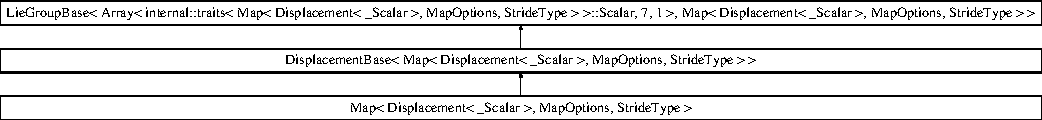
\includegraphics[height=1.612284cm]{class_map_3_01_displacement_3_01___scalar_01_4_00_01_map_options_00_01_stride_type_01_4}
\end{center}
\end{figure}
\subsection*{Public Types}
\begin{DoxyCompactItemize}
\item 
typedef internal\+::traits$<$ \hyperlink{class_map_3_01_displacement_3_01___scalar_01_4_00_01_map_options_00_01_stride_type_01_4_a7355e77dc9b91bd8cb68f20847318f0f}{Map} $>$\+::\hyperlink{class_map_3_01_displacement_3_01___scalar_01_4_00_01_map_options_00_01_stride_type_01_4_a3213feadb99e77889a832a1ef1e80b4b}{Coefficients} \hyperlink{class_map_3_01_displacement_3_01___scalar_01_4_00_01_map_options_00_01_stride_type_01_4_a3213feadb99e77889a832a1ef1e80b4b}{Coefficients}
\end{DoxyCompactItemize}
\subsection*{Public Member Functions}
\begin{DoxyCompactItemize}
\item 
\hyperlink{class_map_3_01_displacement_3_01___scalar_01_4_00_01_map_options_00_01_stride_type_01_4_a7355e77dc9b91bd8cb68f20847318f0f}{Map} (const \hyperlink{class_displacement}{Displacement}$<$ \+\_\+\+Scalar $>$ \&d)
\item 
{\footnotesize template$<$int \+\_\+\+Rows, int \+\_\+\+Cols, int \+\_\+\+Options, int \+\_\+\+Max\+Rows, int \+\_\+\+Max\+Cols$>$ }\\\hyperlink{class_map_3_01_displacement_3_01___scalar_01_4_00_01_map_options_00_01_stride_type_01_4_a711f80d439ccbc921e0b06776d193768}{Map} (const Array$<$ \hyperlink{class_map_3_01_displacement_3_01___scalar_01_4_00_01_map_options_00_01_stride_type_01_4_a1558058db0e90cb7253d6b2dbf414099}{Scalar}, \+\_\+\+Rows, \+\_\+\+Cols, \+\_\+\+Options, \+\_\+\+Max\+Rows, \+\_\+\+Max\+Cols $>$ \&g)
\item 
\hyperlink{class_map_3_01_displacement_3_01___scalar_01_4_00_01_map_options_00_01_stride_type_01_4_ad391569a149b8e0d7c276461901c9425}{Map} (\hyperlink{class_map_3_01_displacement_3_01___scalar_01_4_00_01_map_options_00_01_stride_type_01_4_a1558058db0e90cb7253d6b2dbf414099}{Scalar} $\ast$data)
\item 
\hyperlink{class_map_3_01_displacement_3_01___scalar_01_4_00_01_map_options_00_01_stride_type_01_4_aea0cddfda465eac57cb8914c2d462ad7}{Map} (const Map \&m)
\item 
\hyperlink{class_map_3_01_displacement_3_01___scalar_01_4_00_01_map_options_00_01_stride_type_01_4_a3213feadb99e77889a832a1ef1e80b4b}{Coefficients} \& \hyperlink{class_map_3_01_displacement_3_01___scalar_01_4_00_01_map_options_00_01_stride_type_01_4_a74efdfedea56ddc6344905b30a8f6b5b}{get} ()
\item 
const \hyperlink{class_map_3_01_displacement_3_01___scalar_01_4_00_01_map_options_00_01_stride_type_01_4_a3213feadb99e77889a832a1ef1e80b4b}{Coefficients} \& \hyperlink{class_map_3_01_displacement_3_01___scalar_01_4_00_01_map_options_00_01_stride_type_01_4_a001e7c523f8895fce55047968d4ae80f}{get} () const
\end{DoxyCompactItemize}
\subsection*{Protected Types}
\begin{DoxyCompactItemize}
\item 
typedef \+\_\+\+Scalar \hyperlink{class_map_3_01_displacement_3_01___scalar_01_4_00_01_map_options_00_01_stride_type_01_4_a1558058db0e90cb7253d6b2dbf414099}{Scalar}
\item 
typedef \hyperlink{class_displacement_base}{Displacement\+Base}$<$ \hyperlink{class_map_3_01_displacement_3_01___scalar_01_4_00_01_map_options_00_01_stride_type_01_4_a7355e77dc9b91bd8cb68f20847318f0f}{Map}$<$ \hyperlink{class_displacement}{Displacement}$<$ \hyperlink{class_map_3_01_displacement_3_01___scalar_01_4_00_01_map_options_00_01_stride_type_01_4_a1558058db0e90cb7253d6b2dbf414099}{Scalar} $>$ $>$ $>$ \hyperlink{class_map_3_01_displacement_3_01___scalar_01_4_00_01_map_options_00_01_stride_type_01_4_a1df1fc84e68f902341a4d48037cf82dd}{Base}
\end{DoxyCompactItemize}
\subsection*{Protected Attributes}
\begin{DoxyCompactItemize}
\item 
\hyperlink{class_map_3_01_displacement_3_01___scalar_01_4_00_01_map_options_00_01_stride_type_01_4_a3213feadb99e77889a832a1ef1e80b4b}{Coefficients} \hyperlink{class_map_3_01_displacement_3_01___scalar_01_4_00_01_map_options_00_01_stride_type_01_4_a07b764e529a32d3b74ffc19d4a0949ab}{m\+\_\+coeffs}
\end{DoxyCompactItemize}
\subsection*{Additional Inherited Members}


\subsection{Detailed Description}
\subsubsection*{template$<$typename \+\_\+\+Scalar, int Map\+Options, typename Stride\+Type$>$\newline
class Map$<$ Displacement$<$ \+\_\+\+Scalar $>$, Map\+Options, Stride\+Type $>$}

Class map an array to a rigid \hyperlink{class_displacement}{Displacement} or a 3D Frame position. 


\begin{DoxyTemplParams}{Template Parameters}
{\em \+\_\+\+Scalar} & the type of the underlying array \\
\hline
{\em Map\+Options} & \\
\hline
\end{DoxyTemplParams}
\begin{DoxySeeAlso}{See also}
\hyperlink{class_map_3_01_displacement_3_01___scalar_01_4_00_01_map_options_00_01_stride_type_01_4_a7355e77dc9b91bd8cb68f20847318f0f}{Map$<$\+Matrix$>$} 
\end{DoxySeeAlso}

\begin{DoxyTemplParams}{Template Parameters}
{\em Stride\+Type} & \\
\hline
\end{DoxyTemplParams}
\begin{DoxySeeAlso}{See also}
\hyperlink{class_map_3_01_displacement_3_01___scalar_01_4_00_01_map_options_00_01_stride_type_01_4_a7355e77dc9b91bd8cb68f20847318f0f}{Map$<$\+Matrix$>$}

The methods are defined in \hyperlink{class_lie_group_base}{Lie\+Group\+Base} and \hyperlink{class_displacement_base}{Displacement\+Base} 
\end{DoxySeeAlso}


Definition at line 246 of file Displacement.\+h.



\subsection{Member Typedef Documentation}
\hypertarget{class_map_3_01_displacement_3_01___scalar_01_4_00_01_map_options_00_01_stride_type_01_4_a1df1fc84e68f902341a4d48037cf82dd}{}\label{class_map_3_01_displacement_3_01___scalar_01_4_00_01_map_options_00_01_stride_type_01_4_a1df1fc84e68f902341a4d48037cf82dd} 
\index{Map$<$ Displacement$<$ \+\_\+\+Scalar $>$, Map\+Options, Stride\+Type $>$@{Map$<$ Displacement$<$ \+\_\+\+Scalar $>$, Map\+Options, Stride\+Type $>$}!Base@{Base}}
\index{Base@{Base}!Map$<$ Displacement$<$ \+\_\+\+Scalar $>$, Map\+Options, Stride\+Type $>$@{Map$<$ Displacement$<$ \+\_\+\+Scalar $>$, Map\+Options, Stride\+Type $>$}}
\subsubsection{\texorpdfstring{Base}{Base}}
{\footnotesize\ttfamily template$<$typename \+\_\+\+Scalar , int Map\+Options, typename Stride\+Type $>$ \\
typedef \hyperlink{class_displacement_base}{Displacement\+Base}$<$\hyperlink{class_map_3_01_displacement_3_01___scalar_01_4_00_01_map_options_00_01_stride_type_01_4_a7355e77dc9b91bd8cb68f20847318f0f}{Map}$<$\hyperlink{class_displacement}{Displacement}$<$\hyperlink{class_map_3_01_displacement_3_01___scalar_01_4_00_01_map_options_00_01_stride_type_01_4_a1558058db0e90cb7253d6b2dbf414099}{Scalar}$>$ $>$ $>$ \hyperlink{class_map_3_01_displacement_3_01___scalar_01_4_00_01_map_options_00_01_stride_type_01_4_a7355e77dc9b91bd8cb68f20847318f0f}{Map}$<$ \hyperlink{class_displacement}{Displacement}$<$ \+\_\+\+Scalar $>$, Map\+Options, Stride\+Type $>$\+::\hyperlink{class_map_3_01_displacement_3_01___scalar_01_4_00_01_map_options_00_01_stride_type_01_4_a1df1fc84e68f902341a4d48037cf82dd}{Base}\hspace{0.3cm}{\ttfamily [protected]}}



Definition at line 249 of file Displacement.\+h.

\hypertarget{class_map_3_01_displacement_3_01___scalar_01_4_00_01_map_options_00_01_stride_type_01_4_a3213feadb99e77889a832a1ef1e80b4b}{}\label{class_map_3_01_displacement_3_01___scalar_01_4_00_01_map_options_00_01_stride_type_01_4_a3213feadb99e77889a832a1ef1e80b4b} 
\index{Map$<$ Displacement$<$ \+\_\+\+Scalar $>$, Map\+Options, Stride\+Type $>$@{Map$<$ Displacement$<$ \+\_\+\+Scalar $>$, Map\+Options, Stride\+Type $>$}!Coefficients@{Coefficients}}
\index{Coefficients@{Coefficients}!Map$<$ Displacement$<$ \+\_\+\+Scalar $>$, Map\+Options, Stride\+Type $>$@{Map$<$ Displacement$<$ \+\_\+\+Scalar $>$, Map\+Options, Stride\+Type $>$}}
\subsubsection{\texorpdfstring{Coefficients}{Coefficients}}
{\footnotesize\ttfamily template$<$typename \+\_\+\+Scalar , int Map\+Options, typename Stride\+Type $>$ \\
typedef internal\+::traits$<$\hyperlink{class_map_3_01_displacement_3_01___scalar_01_4_00_01_map_options_00_01_stride_type_01_4_a7355e77dc9b91bd8cb68f20847318f0f}{Map}$>$\+::\hyperlink{class_map_3_01_displacement_3_01___scalar_01_4_00_01_map_options_00_01_stride_type_01_4_a3213feadb99e77889a832a1ef1e80b4b}{Coefficients} \hyperlink{class_map_3_01_displacement_3_01___scalar_01_4_00_01_map_options_00_01_stride_type_01_4_a7355e77dc9b91bd8cb68f20847318f0f}{Map}$<$ \hyperlink{class_displacement}{Displacement}$<$ \+\_\+\+Scalar $>$, Map\+Options, Stride\+Type $>$\+::\hyperlink{class_map_3_01_displacement_3_01___scalar_01_4_00_01_map_options_00_01_stride_type_01_4_a3213feadb99e77889a832a1ef1e80b4b}{Coefficients}}



Definition at line 253 of file Displacement.\+h.

\hypertarget{class_map_3_01_displacement_3_01___scalar_01_4_00_01_map_options_00_01_stride_type_01_4_a1558058db0e90cb7253d6b2dbf414099}{}\label{class_map_3_01_displacement_3_01___scalar_01_4_00_01_map_options_00_01_stride_type_01_4_a1558058db0e90cb7253d6b2dbf414099} 
\index{Map$<$ Displacement$<$ \+\_\+\+Scalar $>$, Map\+Options, Stride\+Type $>$@{Map$<$ Displacement$<$ \+\_\+\+Scalar $>$, Map\+Options, Stride\+Type $>$}!Scalar@{Scalar}}
\index{Scalar@{Scalar}!Map$<$ Displacement$<$ \+\_\+\+Scalar $>$, Map\+Options, Stride\+Type $>$@{Map$<$ Displacement$<$ \+\_\+\+Scalar $>$, Map\+Options, Stride\+Type $>$}}
\subsubsection{\texorpdfstring{Scalar}{Scalar}}
{\footnotesize\ttfamily template$<$typename \+\_\+\+Scalar , int Map\+Options, typename Stride\+Type $>$ \\
typedef \+\_\+\+Scalar \hyperlink{class_map_3_01_displacement_3_01___scalar_01_4_00_01_map_options_00_01_stride_type_01_4_a7355e77dc9b91bd8cb68f20847318f0f}{Map}$<$ \hyperlink{class_displacement}{Displacement}$<$ \+\_\+\+Scalar $>$, Map\+Options, Stride\+Type $>$\+::\hyperlink{class_map_3_01_displacement_3_01___scalar_01_4_00_01_map_options_00_01_stride_type_01_4_a1558058db0e90cb7253d6b2dbf414099}{Scalar}\hspace{0.3cm}{\ttfamily [protected]}}



Definition at line 248 of file Displacement.\+h.



\subsection{Constructor \& Destructor Documentation}
\hypertarget{class_map_3_01_displacement_3_01___scalar_01_4_00_01_map_options_00_01_stride_type_01_4_a7355e77dc9b91bd8cb68f20847318f0f}{}\label{class_map_3_01_displacement_3_01___scalar_01_4_00_01_map_options_00_01_stride_type_01_4_a7355e77dc9b91bd8cb68f20847318f0f} 
\index{Map$<$ Displacement$<$ \+\_\+\+Scalar $>$, Map\+Options, Stride\+Type $>$@{Map$<$ Displacement$<$ \+\_\+\+Scalar $>$, Map\+Options, Stride\+Type $>$}!Map@{Map}}
\index{Map@{Map}!Map$<$ Displacement$<$ \+\_\+\+Scalar $>$, Map\+Options, Stride\+Type $>$@{Map$<$ Displacement$<$ \+\_\+\+Scalar $>$, Map\+Options, Stride\+Type $>$}}
\subsubsection{\texorpdfstring{Map()}{Map()}\hspace{0.1cm}{\footnotesize\ttfamily [1/4]}}
{\footnotesize\ttfamily template$<$typename \+\_\+\+Scalar , int Map\+Options, typename Stride\+Type $>$ \\
Map$<$ \hyperlink{class_displacement}{Displacement}$<$ \+\_\+\+Scalar $>$, Map\+Options, Stride\+Type $>$\+::Map (\begin{DoxyParamCaption}\item[{const \hyperlink{class_displacement}{Displacement}$<$ \+\_\+\+Scalar $>$ \&}]{d }\end{DoxyParamCaption})\hspace{0.3cm}{\ttfamily [inline]}}



Definition at line 255 of file Displacement.\+h.

\hypertarget{class_map_3_01_displacement_3_01___scalar_01_4_00_01_map_options_00_01_stride_type_01_4_a711f80d439ccbc921e0b06776d193768}{}\label{class_map_3_01_displacement_3_01___scalar_01_4_00_01_map_options_00_01_stride_type_01_4_a711f80d439ccbc921e0b06776d193768} 
\index{Map$<$ Displacement$<$ \+\_\+\+Scalar $>$, Map\+Options, Stride\+Type $>$@{Map$<$ Displacement$<$ \+\_\+\+Scalar $>$, Map\+Options, Stride\+Type $>$}!Map@{Map}}
\index{Map@{Map}!Map$<$ Displacement$<$ \+\_\+\+Scalar $>$, Map\+Options, Stride\+Type $>$@{Map$<$ Displacement$<$ \+\_\+\+Scalar $>$, Map\+Options, Stride\+Type $>$}}
\subsubsection{\texorpdfstring{Map()}{Map()}\hspace{0.1cm}{\footnotesize\ttfamily [2/4]}}
{\footnotesize\ttfamily template$<$typename \+\_\+\+Scalar , int Map\+Options, typename Stride\+Type $>$ \\
template$<$int \+\_\+\+Rows, int \+\_\+\+Cols, int \+\_\+\+Options, int \+\_\+\+Max\+Rows, int \+\_\+\+Max\+Cols$>$ \\
Map$<$ \hyperlink{class_displacement}{Displacement}$<$ \+\_\+\+Scalar $>$, Map\+Options, Stride\+Type $>$\+::Map (\begin{DoxyParamCaption}\item[{const Array$<$ \hyperlink{class_map_3_01_displacement_3_01___scalar_01_4_00_01_map_options_00_01_stride_type_01_4_a1558058db0e90cb7253d6b2dbf414099}{Scalar}, \+\_\+\+Rows, \+\_\+\+Cols, \+\_\+\+Options, \+\_\+\+Max\+Rows, \+\_\+\+Max\+Cols $>$ \&}]{g }\end{DoxyParamCaption})\hspace{0.3cm}{\ttfamily [inline]}}



Definition at line 257 of file Displacement.\+h.

\hypertarget{class_map_3_01_displacement_3_01___scalar_01_4_00_01_map_options_00_01_stride_type_01_4_ad391569a149b8e0d7c276461901c9425}{}\label{class_map_3_01_displacement_3_01___scalar_01_4_00_01_map_options_00_01_stride_type_01_4_ad391569a149b8e0d7c276461901c9425} 
\index{Map$<$ Displacement$<$ \+\_\+\+Scalar $>$, Map\+Options, Stride\+Type $>$@{Map$<$ Displacement$<$ \+\_\+\+Scalar $>$, Map\+Options, Stride\+Type $>$}!Map@{Map}}
\index{Map@{Map}!Map$<$ Displacement$<$ \+\_\+\+Scalar $>$, Map\+Options, Stride\+Type $>$@{Map$<$ Displacement$<$ \+\_\+\+Scalar $>$, Map\+Options, Stride\+Type $>$}}
\subsubsection{\texorpdfstring{Map()}{Map()}\hspace{0.1cm}{\footnotesize\ttfamily [3/4]}}
{\footnotesize\ttfamily template$<$typename \+\_\+\+Scalar , int Map\+Options, typename Stride\+Type $>$ \\
Map$<$ \hyperlink{class_displacement}{Displacement}$<$ \+\_\+\+Scalar $>$, Map\+Options, Stride\+Type $>$\+::Map (\begin{DoxyParamCaption}\item[{\hyperlink{class_map_3_01_displacement_3_01___scalar_01_4_00_01_map_options_00_01_stride_type_01_4_a1558058db0e90cb7253d6b2dbf414099}{Scalar} $\ast$}]{data }\end{DoxyParamCaption})\hspace{0.3cm}{\ttfamily [inline]}}



Definition at line 259 of file Displacement.\+h.

\hypertarget{class_map_3_01_displacement_3_01___scalar_01_4_00_01_map_options_00_01_stride_type_01_4_aea0cddfda465eac57cb8914c2d462ad7}{}\label{class_map_3_01_displacement_3_01___scalar_01_4_00_01_map_options_00_01_stride_type_01_4_aea0cddfda465eac57cb8914c2d462ad7} 
\index{Map$<$ Displacement$<$ \+\_\+\+Scalar $>$, Map\+Options, Stride\+Type $>$@{Map$<$ Displacement$<$ \+\_\+\+Scalar $>$, Map\+Options, Stride\+Type $>$}!Map@{Map}}
\index{Map@{Map}!Map$<$ Displacement$<$ \+\_\+\+Scalar $>$, Map\+Options, Stride\+Type $>$@{Map$<$ Displacement$<$ \+\_\+\+Scalar $>$, Map\+Options, Stride\+Type $>$}}
\subsubsection{\texorpdfstring{Map()}{Map()}\hspace{0.1cm}{\footnotesize\ttfamily [4/4]}}
{\footnotesize\ttfamily template$<$typename \+\_\+\+Scalar , int Map\+Options, typename Stride\+Type $>$ \\
Map$<$ \hyperlink{class_displacement}{Displacement}$<$ \+\_\+\+Scalar $>$, Map\+Options, Stride\+Type $>$\+::Map (\begin{DoxyParamCaption}\item[{const Map$<$ \hyperlink{class_displacement}{Displacement}$<$ \+\_\+\+Scalar $>$, Map\+Options, Stride\+Type $>$ \&}]{m }\end{DoxyParamCaption})\hspace{0.3cm}{\ttfamily [inline]}}



Definition at line 260 of file Displacement.\+h.



\subsection{Member Function Documentation}
\hypertarget{class_map_3_01_displacement_3_01___scalar_01_4_00_01_map_options_00_01_stride_type_01_4_a74efdfedea56ddc6344905b30a8f6b5b}{}\label{class_map_3_01_displacement_3_01___scalar_01_4_00_01_map_options_00_01_stride_type_01_4_a74efdfedea56ddc6344905b30a8f6b5b} 
\index{Map$<$ Displacement$<$ \+\_\+\+Scalar $>$, Map\+Options, Stride\+Type $>$@{Map$<$ Displacement$<$ \+\_\+\+Scalar $>$, Map\+Options, Stride\+Type $>$}!get@{get}}
\index{get@{get}!Map$<$ Displacement$<$ \+\_\+\+Scalar $>$, Map\+Options, Stride\+Type $>$@{Map$<$ Displacement$<$ \+\_\+\+Scalar $>$, Map\+Options, Stride\+Type $>$}}
\subsubsection{\texorpdfstring{get()}{get()}\hspace{0.1cm}{\footnotesize\ttfamily [1/2]}}
{\footnotesize\ttfamily template$<$typename \+\_\+\+Scalar , int Map\+Options, typename Stride\+Type $>$ \\
\hyperlink{class_map_3_01_displacement_3_01___scalar_01_4_00_01_map_options_00_01_stride_type_01_4_a3213feadb99e77889a832a1ef1e80b4b}{Coefficients}\& \hyperlink{class_map_3_01_displacement_3_01___scalar_01_4_00_01_map_options_00_01_stride_type_01_4_a7355e77dc9b91bd8cb68f20847318f0f}{Map}$<$ \hyperlink{class_displacement}{Displacement}$<$ \+\_\+\+Scalar $>$, Map\+Options, Stride\+Type $>$\+::get (\begin{DoxyParamCaption}{ }\end{DoxyParamCaption})\hspace{0.3cm}{\ttfamily [inline]}}



Definition at line 262 of file Displacement.\+h.

\hypertarget{class_map_3_01_displacement_3_01___scalar_01_4_00_01_map_options_00_01_stride_type_01_4_a001e7c523f8895fce55047968d4ae80f}{}\label{class_map_3_01_displacement_3_01___scalar_01_4_00_01_map_options_00_01_stride_type_01_4_a001e7c523f8895fce55047968d4ae80f} 
\index{Map$<$ Displacement$<$ \+\_\+\+Scalar $>$, Map\+Options, Stride\+Type $>$@{Map$<$ Displacement$<$ \+\_\+\+Scalar $>$, Map\+Options, Stride\+Type $>$}!get@{get}}
\index{get@{get}!Map$<$ Displacement$<$ \+\_\+\+Scalar $>$, Map\+Options, Stride\+Type $>$@{Map$<$ Displacement$<$ \+\_\+\+Scalar $>$, Map\+Options, Stride\+Type $>$}}
\subsubsection{\texorpdfstring{get()}{get()}\hspace{0.1cm}{\footnotesize\ttfamily [2/2]}}
{\footnotesize\ttfamily template$<$typename \+\_\+\+Scalar , int Map\+Options, typename Stride\+Type $>$ \\
const \hyperlink{class_map_3_01_displacement_3_01___scalar_01_4_00_01_map_options_00_01_stride_type_01_4_a3213feadb99e77889a832a1ef1e80b4b}{Coefficients}\& \hyperlink{class_map_3_01_displacement_3_01___scalar_01_4_00_01_map_options_00_01_stride_type_01_4_a7355e77dc9b91bd8cb68f20847318f0f}{Map}$<$ \hyperlink{class_displacement}{Displacement}$<$ \+\_\+\+Scalar $>$, Map\+Options, Stride\+Type $>$\+::get (\begin{DoxyParamCaption}{ }\end{DoxyParamCaption}) const\hspace{0.3cm}{\ttfamily [inline]}}



Definition at line 263 of file Displacement.\+h.



\subsection{Member Data Documentation}
\hypertarget{class_map_3_01_displacement_3_01___scalar_01_4_00_01_map_options_00_01_stride_type_01_4_a07b764e529a32d3b74ffc19d4a0949ab}{}\label{class_map_3_01_displacement_3_01___scalar_01_4_00_01_map_options_00_01_stride_type_01_4_a07b764e529a32d3b74ffc19d4a0949ab} 
\index{Map$<$ Displacement$<$ \+\_\+\+Scalar $>$, Map\+Options, Stride\+Type $>$@{Map$<$ Displacement$<$ \+\_\+\+Scalar $>$, Map\+Options, Stride\+Type $>$}!m\+\_\+coeffs@{m\+\_\+coeffs}}
\index{m\+\_\+coeffs@{m\+\_\+coeffs}!Map$<$ Displacement$<$ \+\_\+\+Scalar $>$, Map\+Options, Stride\+Type $>$@{Map$<$ Displacement$<$ \+\_\+\+Scalar $>$, Map\+Options, Stride\+Type $>$}}
\subsubsection{\texorpdfstring{m\+\_\+coeffs}{m\_coeffs}}
{\footnotesize\ttfamily template$<$typename \+\_\+\+Scalar , int Map\+Options, typename Stride\+Type $>$ \\
\hyperlink{class_map_3_01_displacement_3_01___scalar_01_4_00_01_map_options_00_01_stride_type_01_4_a3213feadb99e77889a832a1ef1e80b4b}{Coefficients} \hyperlink{class_map_3_01_displacement_3_01___scalar_01_4_00_01_map_options_00_01_stride_type_01_4_a7355e77dc9b91bd8cb68f20847318f0f}{Map}$<$ \hyperlink{class_displacement}{Displacement}$<$ \+\_\+\+Scalar $>$, Map\+Options, Stride\+Type $>$\+::m\+\_\+coeffs\hspace{0.3cm}{\ttfamily [protected]}}



Definition at line 266 of file Displacement.\+h.



The documentation for this class was generated from the following file\+:\begin{DoxyCompactItemize}
\item 
/\+Users/\+Ryan/\+Code/codyco-\/superbuild/libraries/\+Eigen\+Lgsm/unsupported/\+Eigen/src/\+Lgsm/\hyperlink{_displacement_8h}{Displacement.\+h}\end{DoxyCompactItemize}

\hypertarget{class_map_3_01_lie_algebra_3_01_a_01_4_00_01_map_options_00_01_stride_type_01_4}{}\section{Map$<$ Lie\+Algebra$<$ A $>$, Map\+Options, Stride\+Type $>$ Class Template Reference}
\label{class_map_3_01_lie_algebra_3_01_a_01_4_00_01_map_options_00_01_stride_type_01_4}\index{Map$<$ Lie\+Algebra$<$ A $>$, Map\+Options, Stride\+Type $>$@{Map$<$ Lie\+Algebra$<$ A $>$, Map\+Options, Stride\+Type $>$}}


Class describing a map element of a Lie Algebra.  




{\ttfamily \#include $<$Lie\+Algebra.\+h$>$}

Inheritance diagram for Map$<$ Lie\+Algebra$<$ A $>$, Map\+Options, Stride\+Type $>$\+:\begin{figure}[H]
\begin{center}
\leavevmode
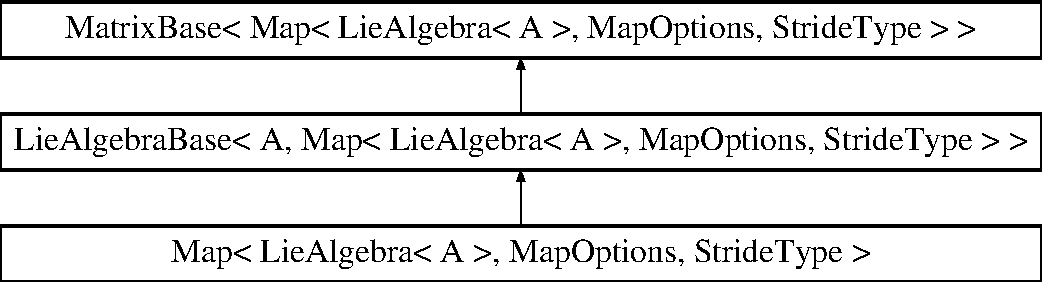
\includegraphics[height=3.000000cm]{class_map_3_01_lie_algebra_3_01_a_01_4_00_01_map_options_00_01_stride_type_01_4}
\end{center}
\end{figure}
\subsection*{Public Types}
\begin{DoxyCompactItemize}
\item 
typedef internal\+::traits$<$ \hyperlink{class_map_3_01_lie_algebra_3_01_a_01_4_00_01_map_options_00_01_stride_type_01_4_a5e320dd14d4d47929d7a4d48014a735f}{Map}$<$ \hyperlink{class_lie_algebra}{Lie\+Algebra}$<$ A $>$, Map\+Options, Stride\+Type $>$ $>$\+::\hyperlink{class_map_3_01_lie_algebra_3_01_a_01_4_00_01_map_options_00_01_stride_type_01_4_a32e1cab48693733071a98e9f558d4c82}{Coefficients} \hyperlink{class_map_3_01_lie_algebra_3_01_a_01_4_00_01_map_options_00_01_stride_type_01_4_a32e1cab48693733071a98e9f558d4c82}{Coefficients}
\end{DoxyCompactItemize}
\subsection*{Public Member Functions}
\begin{DoxyCompactItemize}
\item 
\hyperlink{class_map_3_01_lie_algebra_3_01_a_01_4_00_01_map_options_00_01_stride_type_01_4_a5e320dd14d4d47929d7a4d48014a735f}{Map} (const A \&a)
\item 
\hyperlink{class_map_3_01_lie_algebra_3_01_a_01_4_00_01_map_options_00_01_stride_type_01_4_a5b5a1ddc1058c048c2c202bf3bfd4763}{Map} (Scalar $\ast$data)
\item 
\hyperlink{class_map_3_01_lie_algebra_3_01_a_01_4_00_01_map_options_00_01_stride_type_01_4_a1b4291648994b13392cdc11c4f4d3e2c}{Map} (const Map \&m)
\item 
\hyperlink{class_map_3_01_lie_algebra_3_01_a_01_4_00_01_map_options_00_01_stride_type_01_4_a32e1cab48693733071a98e9f558d4c82}{Coefficients} \& \hyperlink{class_map_3_01_lie_algebra_3_01_a_01_4_00_01_map_options_00_01_stride_type_01_4_af64b17af3736228001fb55f9ed16b5ce}{get} ()
\item 
const \hyperlink{class_map_3_01_lie_algebra_3_01_a_01_4_00_01_map_options_00_01_stride_type_01_4_a32e1cab48693733071a98e9f558d4c82}{Coefficients} \& \hyperlink{class_map_3_01_lie_algebra_3_01_a_01_4_00_01_map_options_00_01_stride_type_01_4_a01a271dce87d94d6fade1279d3f5686f}{get} () const
\end{DoxyCompactItemize}
\subsection*{Protected Types}
\begin{DoxyCompactItemize}
\item 
typedef \hyperlink{class_lie_algebra_base}{Lie\+Algebra\+Base}$<$ A, \hyperlink{class_map_3_01_lie_algebra_3_01_a_01_4_00_01_map_options_00_01_stride_type_01_4_a5e320dd14d4d47929d7a4d48014a735f}{Map}$<$ \hyperlink{class_lie_algebra}{Lie\+Algebra}$<$ A $>$, Map\+Options, Stride\+Type $>$ $>$ \hyperlink{class_map_3_01_lie_algebra_3_01_a_01_4_00_01_map_options_00_01_stride_type_01_4_a1f44b1c76739ca5f9a17c23109c32488}{Base}
\end{DoxyCompactItemize}
\subsection*{Protected Attributes}
\begin{DoxyCompactItemize}
\item 
\hyperlink{class_map_3_01_lie_algebra_3_01_a_01_4_00_01_map_options_00_01_stride_type_01_4_a32e1cab48693733071a98e9f558d4c82}{Coefficients} \hyperlink{class_map_3_01_lie_algebra_3_01_a_01_4_00_01_map_options_00_01_stride_type_01_4_ad9d42724afc3ed4f287a0a3f7a9de6e4}{m\+\_\+coeffs}
\end{DoxyCompactItemize}


\subsection{Detailed Description}
\subsubsection*{template$<$class A, int Map\+Options, typename Stride\+Type$>$\newline
class Map$<$ Lie\+Algebra$<$ A $>$, Map\+Options, Stride\+Type $>$}

Class describing a map element of a Lie Algebra. 

Definition of Map$<$\+Lie\+Algebra$>$


\begin{DoxyTemplParams}{Template Parameters}
{\em G} & the wrapped class \\
\hline
{\em Map\+Options} & \\
\hline
\end{DoxyTemplParams}
\begin{DoxySeeAlso}{See also}
\hyperlink{class_map_3_01_lie_algebra_3_01_a_01_4_00_01_map_options_00_01_stride_type_01_4_a5e320dd14d4d47929d7a4d48014a735f}{Map$<$\+Matrix$>$} 
\end{DoxySeeAlso}

\begin{DoxyTemplParams}{Template Parameters}
{\em Stride\+Type} & \\
\hline
\end{DoxyTemplParams}
\begin{DoxySeeAlso}{See also}
\hyperlink{class_map_3_01_lie_algebra_3_01_a_01_4_00_01_map_options_00_01_stride_type_01_4_a5e320dd14d4d47929d7a4d48014a735f}{Map$<$\+Matrix$>$}
\end{DoxySeeAlso}
This class must be specialized to add new constructors for a specific group.

\begin{DoxySeeAlso}{See also}
The methods are defined in \hyperlink{class_lie_algebra_base}{Lie\+Algebra\+Base} 
\end{DoxySeeAlso}


Definition at line 277 of file Lie\+Algebra.\+h.



\subsection{Member Typedef Documentation}
\hypertarget{class_map_3_01_lie_algebra_3_01_a_01_4_00_01_map_options_00_01_stride_type_01_4_a1f44b1c76739ca5f9a17c23109c32488}{}\label{class_map_3_01_lie_algebra_3_01_a_01_4_00_01_map_options_00_01_stride_type_01_4_a1f44b1c76739ca5f9a17c23109c32488} 
\index{Map$<$ Lie\+Algebra$<$ A $>$, Map\+Options, Stride\+Type $>$@{Map$<$ Lie\+Algebra$<$ A $>$, Map\+Options, Stride\+Type $>$}!Base@{Base}}
\index{Base@{Base}!Map$<$ Lie\+Algebra$<$ A $>$, Map\+Options, Stride\+Type $>$@{Map$<$ Lie\+Algebra$<$ A $>$, Map\+Options, Stride\+Type $>$}}
\subsubsection{\texorpdfstring{Base}{Base}}
{\footnotesize\ttfamily template$<$class A , int Map\+Options, typename Stride\+Type $>$ \\
typedef \hyperlink{class_lie_algebra_base}{Lie\+Algebra\+Base}$<$A, \hyperlink{class_map_3_01_lie_algebra_3_01_a_01_4_00_01_map_options_00_01_stride_type_01_4_a5e320dd14d4d47929d7a4d48014a735f}{Map}$<$\hyperlink{class_lie_algebra}{Lie\+Algebra}$<$A$>$, Map\+Options, Stride\+Type$>$ $>$ \hyperlink{class_map_3_01_lie_algebra_3_01_a_01_4_00_01_map_options_00_01_stride_type_01_4_a5e320dd14d4d47929d7a4d48014a735f}{Map}$<$ \hyperlink{class_lie_algebra}{Lie\+Algebra}$<$ A $>$, Map\+Options, Stride\+Type $>$\+::\hyperlink{class_map_3_01_lie_algebra_3_01_a_01_4_00_01_map_options_00_01_stride_type_01_4_a1f44b1c76739ca5f9a17c23109c32488}{Base}\hspace{0.3cm}{\ttfamily [protected]}}

Inherited class 

Definition at line 280 of file Lie\+Algebra.\+h.

\hypertarget{class_map_3_01_lie_algebra_3_01_a_01_4_00_01_map_options_00_01_stride_type_01_4_a32e1cab48693733071a98e9f558d4c82}{}\label{class_map_3_01_lie_algebra_3_01_a_01_4_00_01_map_options_00_01_stride_type_01_4_a32e1cab48693733071a98e9f558d4c82} 
\index{Map$<$ Lie\+Algebra$<$ A $>$, Map\+Options, Stride\+Type $>$@{Map$<$ Lie\+Algebra$<$ A $>$, Map\+Options, Stride\+Type $>$}!Coefficients@{Coefficients}}
\index{Coefficients@{Coefficients}!Map$<$ Lie\+Algebra$<$ A $>$, Map\+Options, Stride\+Type $>$@{Map$<$ Lie\+Algebra$<$ A $>$, Map\+Options, Stride\+Type $>$}}
\subsubsection{\texorpdfstring{Coefficients}{Coefficients}}
{\footnotesize\ttfamily template$<$class A , int Map\+Options, typename Stride\+Type $>$ \\
typedef internal\+::traits$<$\hyperlink{class_map_3_01_lie_algebra_3_01_a_01_4_00_01_map_options_00_01_stride_type_01_4_a5e320dd14d4d47929d7a4d48014a735f}{Map}$<$\hyperlink{class_lie_algebra}{Lie\+Algebra}$<$A$>$, Map\+Options, Stride\+Type$>$ $>$\+::\hyperlink{class_map_3_01_lie_algebra_3_01_a_01_4_00_01_map_options_00_01_stride_type_01_4_a32e1cab48693733071a98e9f558d4c82}{Coefficients} \hyperlink{class_map_3_01_lie_algebra_3_01_a_01_4_00_01_map_options_00_01_stride_type_01_4_a5e320dd14d4d47929d7a4d48014a735f}{Map}$<$ \hyperlink{class_lie_algebra}{Lie\+Algebra}$<$ A $>$, Map\+Options, Stride\+Type $>$\+::\hyperlink{class_map_3_01_lie_algebra_3_01_a_01_4_00_01_map_options_00_01_stride_type_01_4_a32e1cab48693733071a98e9f558d4c82}{Coefficients}}

The stored coefficients 

Definition at line 288 of file Lie\+Algebra.\+h.



\subsection{Constructor \& Destructor Documentation}
\hypertarget{class_map_3_01_lie_algebra_3_01_a_01_4_00_01_map_options_00_01_stride_type_01_4_a5e320dd14d4d47929d7a4d48014a735f}{}\label{class_map_3_01_lie_algebra_3_01_a_01_4_00_01_map_options_00_01_stride_type_01_4_a5e320dd14d4d47929d7a4d48014a735f} 
\index{Map$<$ Lie\+Algebra$<$ A $>$, Map\+Options, Stride\+Type $>$@{Map$<$ Lie\+Algebra$<$ A $>$, Map\+Options, Stride\+Type $>$}!Map@{Map}}
\index{Map@{Map}!Map$<$ Lie\+Algebra$<$ A $>$, Map\+Options, Stride\+Type $>$@{Map$<$ Lie\+Algebra$<$ A $>$, Map\+Options, Stride\+Type $>$}}
\subsubsection{\texorpdfstring{Map()}{Map()}\hspace{0.1cm}{\footnotesize\ttfamily [1/3]}}
{\footnotesize\ttfamily template$<$class A , int Map\+Options, typename Stride\+Type $>$ \\
Map$<$ \hyperlink{class_lie_algebra}{Lie\+Algebra}$<$ A $>$, Map\+Options, Stride\+Type $>$\+::Map (\begin{DoxyParamCaption}\item[{const A \&}]{a }\end{DoxyParamCaption})\hspace{0.3cm}{\ttfamily [inline]}}

Maps a class A 

Definition at line 291 of file Lie\+Algebra.\+h.

\hypertarget{class_map_3_01_lie_algebra_3_01_a_01_4_00_01_map_options_00_01_stride_type_01_4_a5b5a1ddc1058c048c2c202bf3bfd4763}{}\label{class_map_3_01_lie_algebra_3_01_a_01_4_00_01_map_options_00_01_stride_type_01_4_a5b5a1ddc1058c048c2c202bf3bfd4763} 
\index{Map$<$ Lie\+Algebra$<$ A $>$, Map\+Options, Stride\+Type $>$@{Map$<$ Lie\+Algebra$<$ A $>$, Map\+Options, Stride\+Type $>$}!Map@{Map}}
\index{Map@{Map}!Map$<$ Lie\+Algebra$<$ A $>$, Map\+Options, Stride\+Type $>$@{Map$<$ Lie\+Algebra$<$ A $>$, Map\+Options, Stride\+Type $>$}}
\subsubsection{\texorpdfstring{Map()}{Map()}\hspace{0.1cm}{\footnotesize\ttfamily [2/3]}}
{\footnotesize\ttfamily template$<$class A , int Map\+Options, typename Stride\+Type $>$ \\
Map$<$ \hyperlink{class_lie_algebra}{Lie\+Algebra}$<$ A $>$, Map\+Options, Stride\+Type $>$\+::Map (\begin{DoxyParamCaption}\item[{Scalar $\ast$}]{data }\end{DoxyParamCaption})\hspace{0.3cm}{\ttfamily [inline]}}

Maps an array of scalar 

Definition at line 293 of file Lie\+Algebra.\+h.

\hypertarget{class_map_3_01_lie_algebra_3_01_a_01_4_00_01_map_options_00_01_stride_type_01_4_a1b4291648994b13392cdc11c4f4d3e2c}{}\label{class_map_3_01_lie_algebra_3_01_a_01_4_00_01_map_options_00_01_stride_type_01_4_a1b4291648994b13392cdc11c4f4d3e2c} 
\index{Map$<$ Lie\+Algebra$<$ A $>$, Map\+Options, Stride\+Type $>$@{Map$<$ Lie\+Algebra$<$ A $>$, Map\+Options, Stride\+Type $>$}!Map@{Map}}
\index{Map@{Map}!Map$<$ Lie\+Algebra$<$ A $>$, Map\+Options, Stride\+Type $>$@{Map$<$ Lie\+Algebra$<$ A $>$, Map\+Options, Stride\+Type $>$}}
\subsubsection{\texorpdfstring{Map()}{Map()}\hspace{0.1cm}{\footnotesize\ttfamily [3/3]}}
{\footnotesize\ttfamily template$<$class A , int Map\+Options, typename Stride\+Type $>$ \\
Map$<$ \hyperlink{class_lie_algebra}{Lie\+Algebra}$<$ A $>$, Map\+Options, Stride\+Type $>$\+::Map (\begin{DoxyParamCaption}\item[{const Map$<$ \hyperlink{class_lie_algebra}{Lie\+Algebra}$<$ A $>$, Map\+Options, Stride\+Type $>$ \&}]{m }\end{DoxyParamCaption})\hspace{0.3cm}{\ttfamily [inline]}}

Maps another Map$<$\+Lie\+Algebra$>$ 

Definition at line 295 of file Lie\+Algebra.\+h.



\subsection{Member Function Documentation}
\hypertarget{class_map_3_01_lie_algebra_3_01_a_01_4_00_01_map_options_00_01_stride_type_01_4_af64b17af3736228001fb55f9ed16b5ce}{}\label{class_map_3_01_lie_algebra_3_01_a_01_4_00_01_map_options_00_01_stride_type_01_4_af64b17af3736228001fb55f9ed16b5ce} 
\index{Map$<$ Lie\+Algebra$<$ A $>$, Map\+Options, Stride\+Type $>$@{Map$<$ Lie\+Algebra$<$ A $>$, Map\+Options, Stride\+Type $>$}!get@{get}}
\index{get@{get}!Map$<$ Lie\+Algebra$<$ A $>$, Map\+Options, Stride\+Type $>$@{Map$<$ Lie\+Algebra$<$ A $>$, Map\+Options, Stride\+Type $>$}}
\subsubsection{\texorpdfstring{get()}{get()}\hspace{0.1cm}{\footnotesize\ttfamily [1/2]}}
{\footnotesize\ttfamily template$<$class A , int Map\+Options, typename Stride\+Type $>$ \\
\hyperlink{class_map_3_01_lie_algebra_3_01_a_01_4_00_01_map_options_00_01_stride_type_01_4_a32e1cab48693733071a98e9f558d4c82}{Coefficients}\& \hyperlink{class_map_3_01_lie_algebra_3_01_a_01_4_00_01_map_options_00_01_stride_type_01_4_a5e320dd14d4d47929d7a4d48014a735f}{Map}$<$ \hyperlink{class_lie_algebra}{Lie\+Algebra}$<$ A $>$, Map\+Options, Stride\+Type $>$\+::get (\begin{DoxyParamCaption}{ }\end{DoxyParamCaption})\hspace{0.3cm}{\ttfamily [inline]}}

\begin{DoxyReturn}{Returns}
The stored coefficients 
\end{DoxyReturn}


Definition at line 298 of file Lie\+Algebra.\+h.

\hypertarget{class_map_3_01_lie_algebra_3_01_a_01_4_00_01_map_options_00_01_stride_type_01_4_a01a271dce87d94d6fade1279d3f5686f}{}\label{class_map_3_01_lie_algebra_3_01_a_01_4_00_01_map_options_00_01_stride_type_01_4_a01a271dce87d94d6fade1279d3f5686f} 
\index{Map$<$ Lie\+Algebra$<$ A $>$, Map\+Options, Stride\+Type $>$@{Map$<$ Lie\+Algebra$<$ A $>$, Map\+Options, Stride\+Type $>$}!get@{get}}
\index{get@{get}!Map$<$ Lie\+Algebra$<$ A $>$, Map\+Options, Stride\+Type $>$@{Map$<$ Lie\+Algebra$<$ A $>$, Map\+Options, Stride\+Type $>$}}
\subsubsection{\texorpdfstring{get()}{get()}\hspace{0.1cm}{\footnotesize\ttfamily [2/2]}}
{\footnotesize\ttfamily template$<$class A , int Map\+Options, typename Stride\+Type $>$ \\
const \hyperlink{class_map_3_01_lie_algebra_3_01_a_01_4_00_01_map_options_00_01_stride_type_01_4_a32e1cab48693733071a98e9f558d4c82}{Coefficients}\& \hyperlink{class_map_3_01_lie_algebra_3_01_a_01_4_00_01_map_options_00_01_stride_type_01_4_a5e320dd14d4d47929d7a4d48014a735f}{Map}$<$ \hyperlink{class_lie_algebra}{Lie\+Algebra}$<$ A $>$, Map\+Options, Stride\+Type $>$\+::get (\begin{DoxyParamCaption}{ }\end{DoxyParamCaption}) const\hspace{0.3cm}{\ttfamily [inline]}}

\begin{DoxyReturn}{Returns}
The read-\/only access to the stored coefficients 
\end{DoxyReturn}


Definition at line 300 of file Lie\+Algebra.\+h.



\subsection{Member Data Documentation}
\hypertarget{class_map_3_01_lie_algebra_3_01_a_01_4_00_01_map_options_00_01_stride_type_01_4_ad9d42724afc3ed4f287a0a3f7a9de6e4}{}\label{class_map_3_01_lie_algebra_3_01_a_01_4_00_01_map_options_00_01_stride_type_01_4_ad9d42724afc3ed4f287a0a3f7a9de6e4} 
\index{Map$<$ Lie\+Algebra$<$ A $>$, Map\+Options, Stride\+Type $>$@{Map$<$ Lie\+Algebra$<$ A $>$, Map\+Options, Stride\+Type $>$}!m\+\_\+coeffs@{m\+\_\+coeffs}}
\index{m\+\_\+coeffs@{m\+\_\+coeffs}!Map$<$ Lie\+Algebra$<$ A $>$, Map\+Options, Stride\+Type $>$@{Map$<$ Lie\+Algebra$<$ A $>$, Map\+Options, Stride\+Type $>$}}
\subsubsection{\texorpdfstring{m\+\_\+coeffs}{m\_coeffs}}
{\footnotesize\ttfamily template$<$class A , int Map\+Options, typename Stride\+Type $>$ \\
\hyperlink{class_map_3_01_lie_algebra_3_01_a_01_4_00_01_map_options_00_01_stride_type_01_4_a32e1cab48693733071a98e9f558d4c82}{Coefficients} \hyperlink{class_map_3_01_lie_algebra_3_01_a_01_4_00_01_map_options_00_01_stride_type_01_4_a5e320dd14d4d47929d7a4d48014a735f}{Map}$<$ \hyperlink{class_lie_algebra}{Lie\+Algebra}$<$ A $>$, Map\+Options, Stride\+Type $>$\+::m\+\_\+coeffs\hspace{0.3cm}{\ttfamily [protected]}}

The wrapped coefficients 

Definition at line 304 of file Lie\+Algebra.\+h.



The documentation for this class was generated from the following file\+:\begin{DoxyCompactItemize}
\item 
/\+Users/\+Ryan/\+Code/codyco-\/superbuild/libraries/\+Eigen\+Lgsm/unsupported/\+Eigen/src/\+Lgsm/\hyperlink{_lie_algebra_8h}{Lie\+Algebra.\+h}\end{DoxyCompactItemize}

\hypertarget{class_map_3_01_lie_algebra_dual_3_01_a_01_4_00_01_map_options_00_01_stride_type_01_4}{}\section{Map$<$ Lie\+Algebra\+Dual$<$ A $>$, Map\+Options, Stride\+Type $>$ Class Template Reference}
\label{class_map_3_01_lie_algebra_dual_3_01_a_01_4_00_01_map_options_00_01_stride_type_01_4}\index{Map$<$ Lie\+Algebra\+Dual$<$ A $>$, Map\+Options, Stride\+Type $>$@{Map$<$ Lie\+Algebra\+Dual$<$ A $>$, Map\+Options, Stride\+Type $>$}}


Class describing a map element of a Lie algebra dual..  




{\ttfamily \#include $<$Lie\+Algebra.\+h$>$}

Inheritance diagram for Map$<$ Lie\+Algebra\+Dual$<$ A $>$, Map\+Options, Stride\+Type $>$\+:\begin{figure}[H]
\begin{center}
\leavevmode
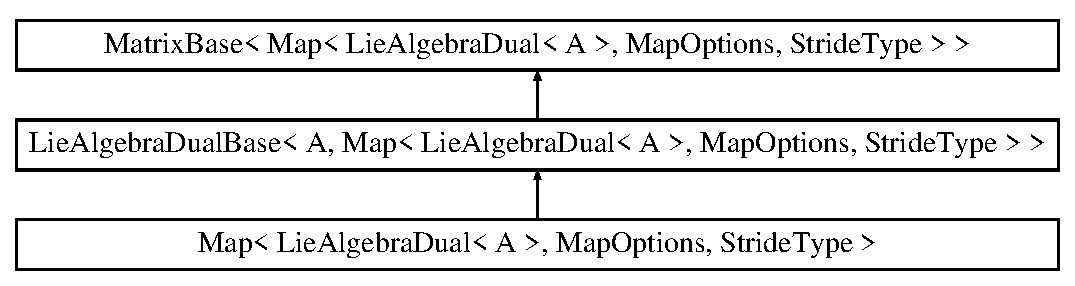
\includegraphics[height=3.000000cm]{class_map_3_01_lie_algebra_dual_3_01_a_01_4_00_01_map_options_00_01_stride_type_01_4}
\end{center}
\end{figure}
\subsection*{Public Types}
\begin{DoxyCompactItemize}
\item 
typedef internal\+::traits$<$ \hyperlink{class_map_3_01_lie_algebra_dual_3_01_a_01_4_00_01_map_options_00_01_stride_type_01_4_a343da7ed6d4069324cd174c8fa51a43f}{Map}$<$ \hyperlink{class_lie_algebra_dual}{Lie\+Algebra\+Dual}$<$ A $>$, Map\+Options, Stride\+Type $>$ $>$\+::\hyperlink{class_map_3_01_lie_algebra_dual_3_01_a_01_4_00_01_map_options_00_01_stride_type_01_4_ab39602ca662c12f4aa9031d05157fb73}{Coefficients} \hyperlink{class_map_3_01_lie_algebra_dual_3_01_a_01_4_00_01_map_options_00_01_stride_type_01_4_ab39602ca662c12f4aa9031d05157fb73}{Coefficients}
\end{DoxyCompactItemize}
\subsection*{Public Member Functions}
\begin{DoxyCompactItemize}
\item 
\hyperlink{class_map_3_01_lie_algebra_dual_3_01_a_01_4_00_01_map_options_00_01_stride_type_01_4_a343da7ed6d4069324cd174c8fa51a43f}{Map} (const A \&a)
\item 
\hyperlink{class_map_3_01_lie_algebra_dual_3_01_a_01_4_00_01_map_options_00_01_stride_type_01_4_abb5e0ae70ea55163f6890a8ccf4be175}{Map} (Scalar $\ast$data)
\item 
\hyperlink{class_map_3_01_lie_algebra_dual_3_01_a_01_4_00_01_map_options_00_01_stride_type_01_4_aebaf7d71c6542435ab56dc9ef7238dce}{Map} (const Map \&m)
\item 
\hyperlink{class_map_3_01_lie_algebra_dual_3_01_a_01_4_00_01_map_options_00_01_stride_type_01_4_ab39602ca662c12f4aa9031d05157fb73}{Coefficients} \& \hyperlink{class_map_3_01_lie_algebra_dual_3_01_a_01_4_00_01_map_options_00_01_stride_type_01_4_a1f2fac20422f722801d08119858da932}{get} ()
\item 
const \hyperlink{class_map_3_01_lie_algebra_dual_3_01_a_01_4_00_01_map_options_00_01_stride_type_01_4_ab39602ca662c12f4aa9031d05157fb73}{Coefficients} \& \hyperlink{class_map_3_01_lie_algebra_dual_3_01_a_01_4_00_01_map_options_00_01_stride_type_01_4_ad394c3da74046cb6660b62e9b7651b2a}{get} () const
\end{DoxyCompactItemize}
\subsection*{Protected Types}
\begin{DoxyCompactItemize}
\item 
typedef \hyperlink{class_lie_algebra_dual_base}{Lie\+Algebra\+Dual\+Base}$<$ A, \hyperlink{class_map_3_01_lie_algebra_dual_3_01_a_01_4_00_01_map_options_00_01_stride_type_01_4_a343da7ed6d4069324cd174c8fa51a43f}{Map}$<$ \hyperlink{class_lie_algebra_dual}{Lie\+Algebra\+Dual}$<$ A $>$, Map\+Options, Stride\+Type $>$ $>$ \hyperlink{class_map_3_01_lie_algebra_dual_3_01_a_01_4_00_01_map_options_00_01_stride_type_01_4_ad1209b4cd7e7831c3556bae3a466822b}{Base}
\end{DoxyCompactItemize}
\subsection*{Protected Attributes}
\begin{DoxyCompactItemize}
\item 
\hyperlink{class_map_3_01_lie_algebra_dual_3_01_a_01_4_00_01_map_options_00_01_stride_type_01_4_ab39602ca662c12f4aa9031d05157fb73}{Coefficients} \hyperlink{class_map_3_01_lie_algebra_dual_3_01_a_01_4_00_01_map_options_00_01_stride_type_01_4_ac9091870e5a828077c30647d4d296c55}{m\+\_\+coeffs}
\end{DoxyCompactItemize}


\subsection{Detailed Description}
\subsubsection*{template$<$class A, int Map\+Options, typename Stride\+Type$>$\newline
class Map$<$ Lie\+Algebra\+Dual$<$ A $>$, Map\+Options, Stride\+Type $>$}

Class describing a map element of a Lie algebra dual.. 

Definition of Map$<$\+Lie\+Algebra\+Dual$>$


\begin{DoxyTemplParams}{Template Parameters}
{\em G} & the wrapped class \\
\hline
{\em Map\+Options} & \\
\hline
\end{DoxyTemplParams}
\begin{DoxySeeAlso}{See also}
\hyperlink{class_map_3_01_lie_algebra_dual_3_01_a_01_4_00_01_map_options_00_01_stride_type_01_4_a343da7ed6d4069324cd174c8fa51a43f}{Map$<$\+Matrix$>$} 
\end{DoxySeeAlso}

\begin{DoxyTemplParams}{Template Parameters}
{\em Stride\+Type} & \\
\hline
\end{DoxyTemplParams}
\begin{DoxySeeAlso}{See also}
\hyperlink{class_map_3_01_lie_algebra_dual_3_01_a_01_4_00_01_map_options_00_01_stride_type_01_4_a343da7ed6d4069324cd174c8fa51a43f}{Map$<$\+Matrix$>$}
\end{DoxySeeAlso}
This class must be specialized to add new constructors for a specific group.

\begin{DoxySeeAlso}{See also}
The methods are defined in \hyperlink{class_lie_algebra_dual_base}{Lie\+Algebra\+Dual\+Base} 
\end{DoxySeeAlso}


Definition at line 370 of file Lie\+Algebra.\+h.



\subsection{Member Typedef Documentation}
\hypertarget{class_map_3_01_lie_algebra_dual_3_01_a_01_4_00_01_map_options_00_01_stride_type_01_4_ad1209b4cd7e7831c3556bae3a466822b}{}\label{class_map_3_01_lie_algebra_dual_3_01_a_01_4_00_01_map_options_00_01_stride_type_01_4_ad1209b4cd7e7831c3556bae3a466822b} 
\index{Map$<$ Lie\+Algebra\+Dual$<$ A $>$, Map\+Options, Stride\+Type $>$@{Map$<$ Lie\+Algebra\+Dual$<$ A $>$, Map\+Options, Stride\+Type $>$}!Base@{Base}}
\index{Base@{Base}!Map$<$ Lie\+Algebra\+Dual$<$ A $>$, Map\+Options, Stride\+Type $>$@{Map$<$ Lie\+Algebra\+Dual$<$ A $>$, Map\+Options, Stride\+Type $>$}}
\subsubsection{\texorpdfstring{Base}{Base}}
{\footnotesize\ttfamily template$<$class A , int Map\+Options, typename Stride\+Type $>$ \\
typedef \hyperlink{class_lie_algebra_dual_base}{Lie\+Algebra\+Dual\+Base}$<$A, \hyperlink{class_map_3_01_lie_algebra_dual_3_01_a_01_4_00_01_map_options_00_01_stride_type_01_4_a343da7ed6d4069324cd174c8fa51a43f}{Map}$<$\hyperlink{class_lie_algebra_dual}{Lie\+Algebra\+Dual}$<$A$>$, Map\+Options, Stride\+Type$>$ $>$ \hyperlink{class_map_3_01_lie_algebra_dual_3_01_a_01_4_00_01_map_options_00_01_stride_type_01_4_a343da7ed6d4069324cd174c8fa51a43f}{Map}$<$ \hyperlink{class_lie_algebra_dual}{Lie\+Algebra\+Dual}$<$ A $>$, Map\+Options, Stride\+Type $>$\+::\hyperlink{class_map_3_01_lie_algebra_dual_3_01_a_01_4_00_01_map_options_00_01_stride_type_01_4_ad1209b4cd7e7831c3556bae3a466822b}{Base}\hspace{0.3cm}{\ttfamily [protected]}}

Inherited class 

Definition at line 373 of file Lie\+Algebra.\+h.

\hypertarget{class_map_3_01_lie_algebra_dual_3_01_a_01_4_00_01_map_options_00_01_stride_type_01_4_ab39602ca662c12f4aa9031d05157fb73}{}\label{class_map_3_01_lie_algebra_dual_3_01_a_01_4_00_01_map_options_00_01_stride_type_01_4_ab39602ca662c12f4aa9031d05157fb73} 
\index{Map$<$ Lie\+Algebra\+Dual$<$ A $>$, Map\+Options, Stride\+Type $>$@{Map$<$ Lie\+Algebra\+Dual$<$ A $>$, Map\+Options, Stride\+Type $>$}!Coefficients@{Coefficients}}
\index{Coefficients@{Coefficients}!Map$<$ Lie\+Algebra\+Dual$<$ A $>$, Map\+Options, Stride\+Type $>$@{Map$<$ Lie\+Algebra\+Dual$<$ A $>$, Map\+Options, Stride\+Type $>$}}
\subsubsection{\texorpdfstring{Coefficients}{Coefficients}}
{\footnotesize\ttfamily template$<$class A , int Map\+Options, typename Stride\+Type $>$ \\
typedef internal\+::traits$<$\hyperlink{class_map_3_01_lie_algebra_dual_3_01_a_01_4_00_01_map_options_00_01_stride_type_01_4_a343da7ed6d4069324cd174c8fa51a43f}{Map}$<$\hyperlink{class_lie_algebra_dual}{Lie\+Algebra\+Dual}$<$A$>$, Map\+Options, Stride\+Type$>$ $>$\+::\hyperlink{class_map_3_01_lie_algebra_dual_3_01_a_01_4_00_01_map_options_00_01_stride_type_01_4_ab39602ca662c12f4aa9031d05157fb73}{Coefficients} \hyperlink{class_map_3_01_lie_algebra_dual_3_01_a_01_4_00_01_map_options_00_01_stride_type_01_4_a343da7ed6d4069324cd174c8fa51a43f}{Map}$<$ \hyperlink{class_lie_algebra_dual}{Lie\+Algebra\+Dual}$<$ A $>$, Map\+Options, Stride\+Type $>$\+::\hyperlink{class_map_3_01_lie_algebra_dual_3_01_a_01_4_00_01_map_options_00_01_stride_type_01_4_ab39602ca662c12f4aa9031d05157fb73}{Coefficients}}

The stored coefficients 

Definition at line 381 of file Lie\+Algebra.\+h.



\subsection{Constructor \& Destructor Documentation}
\hypertarget{class_map_3_01_lie_algebra_dual_3_01_a_01_4_00_01_map_options_00_01_stride_type_01_4_a343da7ed6d4069324cd174c8fa51a43f}{}\label{class_map_3_01_lie_algebra_dual_3_01_a_01_4_00_01_map_options_00_01_stride_type_01_4_a343da7ed6d4069324cd174c8fa51a43f} 
\index{Map$<$ Lie\+Algebra\+Dual$<$ A $>$, Map\+Options, Stride\+Type $>$@{Map$<$ Lie\+Algebra\+Dual$<$ A $>$, Map\+Options, Stride\+Type $>$}!Map@{Map}}
\index{Map@{Map}!Map$<$ Lie\+Algebra\+Dual$<$ A $>$, Map\+Options, Stride\+Type $>$@{Map$<$ Lie\+Algebra\+Dual$<$ A $>$, Map\+Options, Stride\+Type $>$}}
\subsubsection{\texorpdfstring{Map()}{Map()}\hspace{0.1cm}{\footnotesize\ttfamily [1/3]}}
{\footnotesize\ttfamily template$<$class A , int Map\+Options, typename Stride\+Type $>$ \\
Map$<$ \hyperlink{class_lie_algebra_dual}{Lie\+Algebra\+Dual}$<$ A $>$, Map\+Options, Stride\+Type $>$\+::Map (\begin{DoxyParamCaption}\item[{const A \&}]{a }\end{DoxyParamCaption})\hspace{0.3cm}{\ttfamily [inline]}}

Maps a class A 

Definition at line 384 of file Lie\+Algebra.\+h.

\hypertarget{class_map_3_01_lie_algebra_dual_3_01_a_01_4_00_01_map_options_00_01_stride_type_01_4_abb5e0ae70ea55163f6890a8ccf4be175}{}\label{class_map_3_01_lie_algebra_dual_3_01_a_01_4_00_01_map_options_00_01_stride_type_01_4_abb5e0ae70ea55163f6890a8ccf4be175} 
\index{Map$<$ Lie\+Algebra\+Dual$<$ A $>$, Map\+Options, Stride\+Type $>$@{Map$<$ Lie\+Algebra\+Dual$<$ A $>$, Map\+Options, Stride\+Type $>$}!Map@{Map}}
\index{Map@{Map}!Map$<$ Lie\+Algebra\+Dual$<$ A $>$, Map\+Options, Stride\+Type $>$@{Map$<$ Lie\+Algebra\+Dual$<$ A $>$, Map\+Options, Stride\+Type $>$}}
\subsubsection{\texorpdfstring{Map()}{Map()}\hspace{0.1cm}{\footnotesize\ttfamily [2/3]}}
{\footnotesize\ttfamily template$<$class A , int Map\+Options, typename Stride\+Type $>$ \\
Map$<$ \hyperlink{class_lie_algebra_dual}{Lie\+Algebra\+Dual}$<$ A $>$, Map\+Options, Stride\+Type $>$\+::Map (\begin{DoxyParamCaption}\item[{Scalar $\ast$}]{data }\end{DoxyParamCaption})\hspace{0.3cm}{\ttfamily [inline]}}

Maps an array of scalar 

Definition at line 386 of file Lie\+Algebra.\+h.

\hypertarget{class_map_3_01_lie_algebra_dual_3_01_a_01_4_00_01_map_options_00_01_stride_type_01_4_aebaf7d71c6542435ab56dc9ef7238dce}{}\label{class_map_3_01_lie_algebra_dual_3_01_a_01_4_00_01_map_options_00_01_stride_type_01_4_aebaf7d71c6542435ab56dc9ef7238dce} 
\index{Map$<$ Lie\+Algebra\+Dual$<$ A $>$, Map\+Options, Stride\+Type $>$@{Map$<$ Lie\+Algebra\+Dual$<$ A $>$, Map\+Options, Stride\+Type $>$}!Map@{Map}}
\index{Map@{Map}!Map$<$ Lie\+Algebra\+Dual$<$ A $>$, Map\+Options, Stride\+Type $>$@{Map$<$ Lie\+Algebra\+Dual$<$ A $>$, Map\+Options, Stride\+Type $>$}}
\subsubsection{\texorpdfstring{Map()}{Map()}\hspace{0.1cm}{\footnotesize\ttfamily [3/3]}}
{\footnotesize\ttfamily template$<$class A , int Map\+Options, typename Stride\+Type $>$ \\
Map$<$ \hyperlink{class_lie_algebra_dual}{Lie\+Algebra\+Dual}$<$ A $>$, Map\+Options, Stride\+Type $>$\+::Map (\begin{DoxyParamCaption}\item[{const Map$<$ \hyperlink{class_lie_algebra_dual}{Lie\+Algebra\+Dual}$<$ A $>$, Map\+Options, Stride\+Type $>$ \&}]{m }\end{DoxyParamCaption})\hspace{0.3cm}{\ttfamily [inline]}}

Maps another Map$<$\+Lie\+Algebra$>$ 

Definition at line 388 of file Lie\+Algebra.\+h.



\subsection{Member Function Documentation}
\hypertarget{class_map_3_01_lie_algebra_dual_3_01_a_01_4_00_01_map_options_00_01_stride_type_01_4_a1f2fac20422f722801d08119858da932}{}\label{class_map_3_01_lie_algebra_dual_3_01_a_01_4_00_01_map_options_00_01_stride_type_01_4_a1f2fac20422f722801d08119858da932} 
\index{Map$<$ Lie\+Algebra\+Dual$<$ A $>$, Map\+Options, Stride\+Type $>$@{Map$<$ Lie\+Algebra\+Dual$<$ A $>$, Map\+Options, Stride\+Type $>$}!get@{get}}
\index{get@{get}!Map$<$ Lie\+Algebra\+Dual$<$ A $>$, Map\+Options, Stride\+Type $>$@{Map$<$ Lie\+Algebra\+Dual$<$ A $>$, Map\+Options, Stride\+Type $>$}}
\subsubsection{\texorpdfstring{get()}{get()}\hspace{0.1cm}{\footnotesize\ttfamily [1/2]}}
{\footnotesize\ttfamily template$<$class A , int Map\+Options, typename Stride\+Type $>$ \\
\hyperlink{class_map_3_01_lie_algebra_dual_3_01_a_01_4_00_01_map_options_00_01_stride_type_01_4_ab39602ca662c12f4aa9031d05157fb73}{Coefficients}\& \hyperlink{class_map_3_01_lie_algebra_dual_3_01_a_01_4_00_01_map_options_00_01_stride_type_01_4_a343da7ed6d4069324cd174c8fa51a43f}{Map}$<$ \hyperlink{class_lie_algebra_dual}{Lie\+Algebra\+Dual}$<$ A $>$, Map\+Options, Stride\+Type $>$\+::get (\begin{DoxyParamCaption}{ }\end{DoxyParamCaption})\hspace{0.3cm}{\ttfamily [inline]}}

\begin{DoxyReturn}{Returns}
The stored coefficients 
\end{DoxyReturn}


Definition at line 391 of file Lie\+Algebra.\+h.

\hypertarget{class_map_3_01_lie_algebra_dual_3_01_a_01_4_00_01_map_options_00_01_stride_type_01_4_ad394c3da74046cb6660b62e9b7651b2a}{}\label{class_map_3_01_lie_algebra_dual_3_01_a_01_4_00_01_map_options_00_01_stride_type_01_4_ad394c3da74046cb6660b62e9b7651b2a} 
\index{Map$<$ Lie\+Algebra\+Dual$<$ A $>$, Map\+Options, Stride\+Type $>$@{Map$<$ Lie\+Algebra\+Dual$<$ A $>$, Map\+Options, Stride\+Type $>$}!get@{get}}
\index{get@{get}!Map$<$ Lie\+Algebra\+Dual$<$ A $>$, Map\+Options, Stride\+Type $>$@{Map$<$ Lie\+Algebra\+Dual$<$ A $>$, Map\+Options, Stride\+Type $>$}}
\subsubsection{\texorpdfstring{get()}{get()}\hspace{0.1cm}{\footnotesize\ttfamily [2/2]}}
{\footnotesize\ttfamily template$<$class A , int Map\+Options, typename Stride\+Type $>$ \\
const \hyperlink{class_map_3_01_lie_algebra_dual_3_01_a_01_4_00_01_map_options_00_01_stride_type_01_4_ab39602ca662c12f4aa9031d05157fb73}{Coefficients}\& \hyperlink{class_map_3_01_lie_algebra_dual_3_01_a_01_4_00_01_map_options_00_01_stride_type_01_4_a343da7ed6d4069324cd174c8fa51a43f}{Map}$<$ \hyperlink{class_lie_algebra_dual}{Lie\+Algebra\+Dual}$<$ A $>$, Map\+Options, Stride\+Type $>$\+::get (\begin{DoxyParamCaption}{ }\end{DoxyParamCaption}) const\hspace{0.3cm}{\ttfamily [inline]}}

\begin{DoxyReturn}{Returns}
The read-\/only access to the stored coefficients 
\end{DoxyReturn}


Definition at line 393 of file Lie\+Algebra.\+h.



\subsection{Member Data Documentation}
\hypertarget{class_map_3_01_lie_algebra_dual_3_01_a_01_4_00_01_map_options_00_01_stride_type_01_4_ac9091870e5a828077c30647d4d296c55}{}\label{class_map_3_01_lie_algebra_dual_3_01_a_01_4_00_01_map_options_00_01_stride_type_01_4_ac9091870e5a828077c30647d4d296c55} 
\index{Map$<$ Lie\+Algebra\+Dual$<$ A $>$, Map\+Options, Stride\+Type $>$@{Map$<$ Lie\+Algebra\+Dual$<$ A $>$, Map\+Options, Stride\+Type $>$}!m\+\_\+coeffs@{m\+\_\+coeffs}}
\index{m\+\_\+coeffs@{m\+\_\+coeffs}!Map$<$ Lie\+Algebra\+Dual$<$ A $>$, Map\+Options, Stride\+Type $>$@{Map$<$ Lie\+Algebra\+Dual$<$ A $>$, Map\+Options, Stride\+Type $>$}}
\subsubsection{\texorpdfstring{m\+\_\+coeffs}{m\_coeffs}}
{\footnotesize\ttfamily template$<$class A , int Map\+Options, typename Stride\+Type $>$ \\
\hyperlink{class_map_3_01_lie_algebra_dual_3_01_a_01_4_00_01_map_options_00_01_stride_type_01_4_ab39602ca662c12f4aa9031d05157fb73}{Coefficients} \hyperlink{class_map_3_01_lie_algebra_dual_3_01_a_01_4_00_01_map_options_00_01_stride_type_01_4_a343da7ed6d4069324cd174c8fa51a43f}{Map}$<$ \hyperlink{class_lie_algebra_dual}{Lie\+Algebra\+Dual}$<$ A $>$, Map\+Options, Stride\+Type $>$\+::m\+\_\+coeffs\hspace{0.3cm}{\ttfamily [protected]}}

The wrapped coefficients 

Definition at line 397 of file Lie\+Algebra.\+h.



The documentation for this class was generated from the following file\+:\begin{DoxyCompactItemize}
\item 
/\+Users/\+Ryan/\+Code/codyco-\/superbuild/libraries/\+Eigen\+Lgsm/unsupported/\+Eigen/src/\+Lgsm/\hyperlink{_lie_algebra_8h}{Lie\+Algebra.\+h}\end{DoxyCompactItemize}

\hypertarget{class_map_3_01_lie_group_3_01_g_01_4_00_01_map_options_00_01_stride_type_01_4}{}\section{Map$<$ Lie\+Group$<$ G $>$, Map\+Options, Stride\+Type $>$ Class Template Reference}
\label{class_map_3_01_lie_group_3_01_g_01_4_00_01_map_options_00_01_stride_type_01_4}\index{Map$<$ Lie\+Group$<$ G $>$, Map\+Options, Stride\+Type $>$@{Map$<$ Lie\+Group$<$ G $>$, Map\+Options, Stride\+Type $>$}}


Class describing a map element of a Lie Group.  




{\ttfamily \#include $<$Lie\+Group.\+h$>$}

Inheritance diagram for Map$<$ Lie\+Group$<$ G $>$, Map\+Options, Stride\+Type $>$\+:\begin{figure}[H]
\begin{center}
\leavevmode
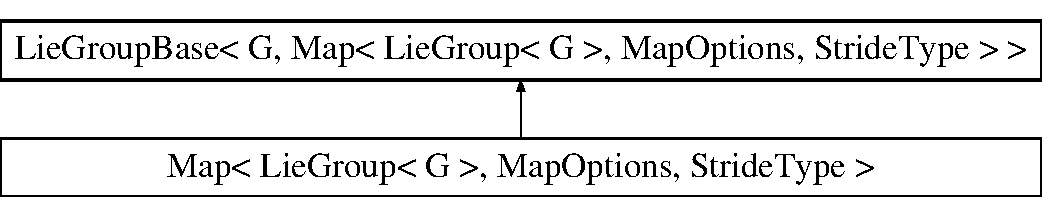
\includegraphics[height=2.000000cm]{class_map_3_01_lie_group_3_01_g_01_4_00_01_map_options_00_01_stride_type_01_4}
\end{center}
\end{figure}
\subsection*{Public Types}
\begin{DoxyCompactItemize}
\item 
typedef internal\+::traits$<$ \hyperlink{class_map_3_01_lie_group_3_01_g_01_4_00_01_map_options_00_01_stride_type_01_4_a141753f9a4186911b53b5b25cfd716ed}{Map}$<$ \hyperlink{class_lie_group}{Lie\+Group}$<$ G $>$, Map\+Options, Stride\+Type $>$ $>$\+::\hyperlink{class_map_3_01_lie_group_3_01_g_01_4_00_01_map_options_00_01_stride_type_01_4_ac0fdd69f3b12cdc0b88be71c2283e9ae}{Scalar} \hyperlink{class_map_3_01_lie_group_3_01_g_01_4_00_01_map_options_00_01_stride_type_01_4_ac0fdd69f3b12cdc0b88be71c2283e9ae}{Scalar}
\item 
typedef internal\+::traits$<$ \hyperlink{class_map_3_01_lie_group_3_01_g_01_4_00_01_map_options_00_01_stride_type_01_4_a141753f9a4186911b53b5b25cfd716ed}{Map}$<$ \hyperlink{class_lie_group}{Lie\+Group}$<$ G $>$, Map\+Options, Stride\+Type $>$ $>$\+::\hyperlink{class_map_3_01_lie_group_3_01_g_01_4_00_01_map_options_00_01_stride_type_01_4_a3140b440390b3c15c7361ab182a91f91}{Coefficients} \hyperlink{class_map_3_01_lie_group_3_01_g_01_4_00_01_map_options_00_01_stride_type_01_4_a3140b440390b3c15c7361ab182a91f91}{Coefficients}
\end{DoxyCompactItemize}
\subsection*{Public Member Functions}
\begin{DoxyCompactItemize}
\item 
\hyperlink{class_map_3_01_lie_group_3_01_g_01_4_00_01_map_options_00_01_stride_type_01_4_a141753f9a4186911b53b5b25cfd716ed}{Map} (const G \&g)
\item 
{\footnotesize template$<$int \+\_\+\+Rows, int \+\_\+\+Cols, int \+\_\+\+Options, int \+\_\+\+Max\+Rows, int \+\_\+\+Max\+Cols$>$ }\\\hyperlink{class_map_3_01_lie_group_3_01_g_01_4_00_01_map_options_00_01_stride_type_01_4_a33f366f2a0c009b10b35c531ee71dcb9}{Map} (Array$<$ \hyperlink{class_map_3_01_lie_group_3_01_g_01_4_00_01_map_options_00_01_stride_type_01_4_ac0fdd69f3b12cdc0b88be71c2283e9ae}{Scalar}, \+\_\+\+Rows, \+\_\+\+Cols, \+\_\+\+Options, \+\_\+\+Max\+Rows, \+\_\+\+Max\+Cols $>$ \&g)
\item 
\hyperlink{class_map_3_01_lie_group_3_01_g_01_4_00_01_map_options_00_01_stride_type_01_4_a06e9c15966f1be0bfefcadb3c8c74ad4}{Map} (\hyperlink{class_map_3_01_lie_group_3_01_g_01_4_00_01_map_options_00_01_stride_type_01_4_ac0fdd69f3b12cdc0b88be71c2283e9ae}{Scalar} $\ast$data)
\item 
\hyperlink{class_map_3_01_lie_group_3_01_g_01_4_00_01_map_options_00_01_stride_type_01_4_ae6280fe976a1f7d0a60ee211a2530857}{Map} (const Map \&m)
\item 
\hyperlink{class_map_3_01_lie_group_3_01_g_01_4_00_01_map_options_00_01_stride_type_01_4_a3140b440390b3c15c7361ab182a91f91}{Coefficients} \& \hyperlink{class_map_3_01_lie_group_3_01_g_01_4_00_01_map_options_00_01_stride_type_01_4_afdbf1ac5998b66bf071097cbc645b61c}{get} ()
\item 
const \hyperlink{class_map_3_01_lie_group_3_01_g_01_4_00_01_map_options_00_01_stride_type_01_4_a3140b440390b3c15c7361ab182a91f91}{Coefficients} \& \hyperlink{class_map_3_01_lie_group_3_01_g_01_4_00_01_map_options_00_01_stride_type_01_4_a6e202f2f5d1ba37f2b2a414bfa70a7e8}{get} () const
\end{DoxyCompactItemize}
\subsection*{Protected Types}
\begin{DoxyCompactItemize}
\item 
typedef \hyperlink{class_lie_group_base}{Lie\+Group\+Base}$<$ G, \hyperlink{class_map_3_01_lie_group_3_01_g_01_4_00_01_map_options_00_01_stride_type_01_4_a141753f9a4186911b53b5b25cfd716ed}{Map}$<$ \hyperlink{class_lie_group}{Lie\+Group}$<$ G $>$, Map\+Options, Stride\+Type $>$ $>$ \hyperlink{class_map_3_01_lie_group_3_01_g_01_4_00_01_map_options_00_01_stride_type_01_4_a09cb088c0990b2ab5558a5ecd245f2c4}{Base}
\end{DoxyCompactItemize}
\subsection*{Protected Attributes}
\begin{DoxyCompactItemize}
\item 
\hyperlink{class_map_3_01_lie_group_3_01_g_01_4_00_01_map_options_00_01_stride_type_01_4_a3140b440390b3c15c7361ab182a91f91}{Coefficients} \hyperlink{class_map_3_01_lie_group_3_01_g_01_4_00_01_map_options_00_01_stride_type_01_4_ab567fb9415879d9fa0fcf35465dc0beb}{m\+\_\+coeffs}
\end{DoxyCompactItemize}
\subsection*{Additional Inherited Members}


\subsection{Detailed Description}
\subsubsection*{template$<$class G, int Map\+Options, typename Stride\+Type$>$\newline
class Map$<$ Lie\+Group$<$ G $>$, Map\+Options, Stride\+Type $>$}

Class describing a map element of a Lie Group. 

Definition of Map$<$\+Lie\+Group$>$


\begin{DoxyTemplParams}{Template Parameters}
{\em G} & the wrapped class \\
\hline
{\em Map\+Options} & \\
\hline
\end{DoxyTemplParams}
\begin{DoxySeeAlso}{See also}
\hyperlink{class_map_3_01_lie_group_3_01_g_01_4_00_01_map_options_00_01_stride_type_01_4_a141753f9a4186911b53b5b25cfd716ed}{Map$<$\+Matrix$>$} 
\end{DoxySeeAlso}

\begin{DoxyTemplParams}{Template Parameters}
{\em Stride\+Type} & \\
\hline
\end{DoxyTemplParams}
\begin{DoxySeeAlso}{See also}
\hyperlink{class_map_3_01_lie_group_3_01_g_01_4_00_01_map_options_00_01_stride_type_01_4_a141753f9a4186911b53b5b25cfd716ed}{Map$<$\+Matrix$>$}
\end{DoxySeeAlso}
This class must be specialized to add new constructors for a specific group.

\begin{DoxySeeAlso}{See also}
The methods are defined in \hyperlink{class_lie_group_base}{Lie\+Group\+Base} 
\end{DoxySeeAlso}


Definition at line 178 of file Lie\+Group.\+h.



\subsection{Member Typedef Documentation}
\hypertarget{class_map_3_01_lie_group_3_01_g_01_4_00_01_map_options_00_01_stride_type_01_4_a09cb088c0990b2ab5558a5ecd245f2c4}{}\label{class_map_3_01_lie_group_3_01_g_01_4_00_01_map_options_00_01_stride_type_01_4_a09cb088c0990b2ab5558a5ecd245f2c4} 
\index{Map$<$ Lie\+Group$<$ G $>$, Map\+Options, Stride\+Type $>$@{Map$<$ Lie\+Group$<$ G $>$, Map\+Options, Stride\+Type $>$}!Base@{Base}}
\index{Base@{Base}!Map$<$ Lie\+Group$<$ G $>$, Map\+Options, Stride\+Type $>$@{Map$<$ Lie\+Group$<$ G $>$, Map\+Options, Stride\+Type $>$}}
\subsubsection{\texorpdfstring{Base}{Base}}
{\footnotesize\ttfamily template$<$class G , int Map\+Options, typename Stride\+Type $>$ \\
typedef \hyperlink{class_lie_group_base}{Lie\+Group\+Base}$<$G, \hyperlink{class_map_3_01_lie_group_3_01_g_01_4_00_01_map_options_00_01_stride_type_01_4_a141753f9a4186911b53b5b25cfd716ed}{Map}$<$\hyperlink{class_lie_group}{Lie\+Group}$<$G$>$, Map\+Options, Stride\+Type $>$ $>$ \hyperlink{class_map_3_01_lie_group_3_01_g_01_4_00_01_map_options_00_01_stride_type_01_4_a141753f9a4186911b53b5b25cfd716ed}{Map}$<$ \hyperlink{class_lie_group}{Lie\+Group}$<$ G $>$, Map\+Options, Stride\+Type $>$\+::\hyperlink{class_map_3_01_lie_group_3_01_g_01_4_00_01_map_options_00_01_stride_type_01_4_a09cb088c0990b2ab5558a5ecd245f2c4}{Base}\hspace{0.3cm}{\ttfamily [protected]}}

Inherited class 

Definition at line 181 of file Lie\+Group.\+h.

\hypertarget{class_map_3_01_lie_group_3_01_g_01_4_00_01_map_options_00_01_stride_type_01_4_a3140b440390b3c15c7361ab182a91f91}{}\label{class_map_3_01_lie_group_3_01_g_01_4_00_01_map_options_00_01_stride_type_01_4_a3140b440390b3c15c7361ab182a91f91} 
\index{Map$<$ Lie\+Group$<$ G $>$, Map\+Options, Stride\+Type $>$@{Map$<$ Lie\+Group$<$ G $>$, Map\+Options, Stride\+Type $>$}!Coefficients@{Coefficients}}
\index{Coefficients@{Coefficients}!Map$<$ Lie\+Group$<$ G $>$, Map\+Options, Stride\+Type $>$@{Map$<$ Lie\+Group$<$ G $>$, Map\+Options, Stride\+Type $>$}}
\subsubsection{\texorpdfstring{Coefficients}{Coefficients}}
{\footnotesize\ttfamily template$<$class G , int Map\+Options, typename Stride\+Type $>$ \\
typedef internal\+::traits$<$\hyperlink{class_map_3_01_lie_group_3_01_g_01_4_00_01_map_options_00_01_stride_type_01_4_a141753f9a4186911b53b5b25cfd716ed}{Map}$<$\hyperlink{class_lie_group}{Lie\+Group}$<$G$>$, Map\+Options, Stride\+Type$>$ $>$\+::\hyperlink{class_map_3_01_lie_group_3_01_g_01_4_00_01_map_options_00_01_stride_type_01_4_a3140b440390b3c15c7361ab182a91f91}{Coefficients} \hyperlink{class_map_3_01_lie_group_3_01_g_01_4_00_01_map_options_00_01_stride_type_01_4_a141753f9a4186911b53b5b25cfd716ed}{Map}$<$ \hyperlink{class_lie_group}{Lie\+Group}$<$ G $>$, Map\+Options, Stride\+Type $>$\+::\hyperlink{class_map_3_01_lie_group_3_01_g_01_4_00_01_map_options_00_01_stride_type_01_4_a3140b440390b3c15c7361ab182a91f91}{Coefficients}}

The stored coefficients 

Definition at line 188 of file Lie\+Group.\+h.

\hypertarget{class_map_3_01_lie_group_3_01_g_01_4_00_01_map_options_00_01_stride_type_01_4_ac0fdd69f3b12cdc0b88be71c2283e9ae}{}\label{class_map_3_01_lie_group_3_01_g_01_4_00_01_map_options_00_01_stride_type_01_4_ac0fdd69f3b12cdc0b88be71c2283e9ae} 
\index{Map$<$ Lie\+Group$<$ G $>$, Map\+Options, Stride\+Type $>$@{Map$<$ Lie\+Group$<$ G $>$, Map\+Options, Stride\+Type $>$}!Scalar@{Scalar}}
\index{Scalar@{Scalar}!Map$<$ Lie\+Group$<$ G $>$, Map\+Options, Stride\+Type $>$@{Map$<$ Lie\+Group$<$ G $>$, Map\+Options, Stride\+Type $>$}}
\subsubsection{\texorpdfstring{Scalar}{Scalar}}
{\footnotesize\ttfamily template$<$class G , int Map\+Options, typename Stride\+Type $>$ \\
typedef internal\+::traits$<$\hyperlink{class_map_3_01_lie_group_3_01_g_01_4_00_01_map_options_00_01_stride_type_01_4_a141753f9a4186911b53b5b25cfd716ed}{Map}$<$\hyperlink{class_lie_group}{Lie\+Group}$<$G$>$, Map\+Options, Stride\+Type$>$ $>$\+::\hyperlink{class_map_3_01_lie_group_3_01_g_01_4_00_01_map_options_00_01_stride_type_01_4_ac0fdd69f3b12cdc0b88be71c2283e9ae}{Scalar} \hyperlink{class_map_3_01_lie_group_3_01_g_01_4_00_01_map_options_00_01_stride_type_01_4_a141753f9a4186911b53b5b25cfd716ed}{Map}$<$ \hyperlink{class_lie_group}{Lie\+Group}$<$ G $>$, Map\+Options, Stride\+Type $>$\+::\hyperlink{class_map_3_01_lie_group_3_01_g_01_4_00_01_map_options_00_01_stride_type_01_4_ac0fdd69f3b12cdc0b88be71c2283e9ae}{Scalar}}

Coefficients type 

Definition at line 186 of file Lie\+Group.\+h.



\subsection{Constructor \& Destructor Documentation}
\hypertarget{class_map_3_01_lie_group_3_01_g_01_4_00_01_map_options_00_01_stride_type_01_4_a141753f9a4186911b53b5b25cfd716ed}{}\label{class_map_3_01_lie_group_3_01_g_01_4_00_01_map_options_00_01_stride_type_01_4_a141753f9a4186911b53b5b25cfd716ed} 
\index{Map$<$ Lie\+Group$<$ G $>$, Map\+Options, Stride\+Type $>$@{Map$<$ Lie\+Group$<$ G $>$, Map\+Options, Stride\+Type $>$}!Map@{Map}}
\index{Map@{Map}!Map$<$ Lie\+Group$<$ G $>$, Map\+Options, Stride\+Type $>$@{Map$<$ Lie\+Group$<$ G $>$, Map\+Options, Stride\+Type $>$}}
\subsubsection{\texorpdfstring{Map()}{Map()}\hspace{0.1cm}{\footnotesize\ttfamily [1/4]}}
{\footnotesize\ttfamily template$<$class G , int Map\+Options, typename Stride\+Type $>$ \\
Map$<$ \hyperlink{class_lie_group}{Lie\+Group}$<$ G $>$, Map\+Options, Stride\+Type $>$\+::Map (\begin{DoxyParamCaption}\item[{const G \&}]{g }\end{DoxyParamCaption})\hspace{0.3cm}{\ttfamily [inline]}}

Maps a class G 

Definition at line 191 of file Lie\+Group.\+h.

\hypertarget{class_map_3_01_lie_group_3_01_g_01_4_00_01_map_options_00_01_stride_type_01_4_a33f366f2a0c009b10b35c531ee71dcb9}{}\label{class_map_3_01_lie_group_3_01_g_01_4_00_01_map_options_00_01_stride_type_01_4_a33f366f2a0c009b10b35c531ee71dcb9} 
\index{Map$<$ Lie\+Group$<$ G $>$, Map\+Options, Stride\+Type $>$@{Map$<$ Lie\+Group$<$ G $>$, Map\+Options, Stride\+Type $>$}!Map@{Map}}
\index{Map@{Map}!Map$<$ Lie\+Group$<$ G $>$, Map\+Options, Stride\+Type $>$@{Map$<$ Lie\+Group$<$ G $>$, Map\+Options, Stride\+Type $>$}}
\subsubsection{\texorpdfstring{Map()}{Map()}\hspace{0.1cm}{\footnotesize\ttfamily [2/4]}}
{\footnotesize\ttfamily template$<$class G , int Map\+Options, typename Stride\+Type $>$ \\
template$<$int \+\_\+\+Rows, int \+\_\+\+Cols, int \+\_\+\+Options, int \+\_\+\+Max\+Rows, int \+\_\+\+Max\+Cols$>$ \\
Map$<$ \hyperlink{class_lie_group}{Lie\+Group}$<$ G $>$, Map\+Options, Stride\+Type $>$\+::Map (\begin{DoxyParamCaption}\item[{Array$<$ \hyperlink{class_map_3_01_lie_group_3_01_g_01_4_00_01_map_options_00_01_stride_type_01_4_ac0fdd69f3b12cdc0b88be71c2283e9ae}{Scalar}, \+\_\+\+Rows, \+\_\+\+Cols, \+\_\+\+Options, \+\_\+\+Max\+Rows, \+\_\+\+Max\+Cols $>$ \&}]{g }\end{DoxyParamCaption})\hspace{0.3cm}{\ttfamily [inline]}}

Maps an Array 

Definition at line 194 of file Lie\+Group.\+h.

\hypertarget{class_map_3_01_lie_group_3_01_g_01_4_00_01_map_options_00_01_stride_type_01_4_a06e9c15966f1be0bfefcadb3c8c74ad4}{}\label{class_map_3_01_lie_group_3_01_g_01_4_00_01_map_options_00_01_stride_type_01_4_a06e9c15966f1be0bfefcadb3c8c74ad4} 
\index{Map$<$ Lie\+Group$<$ G $>$, Map\+Options, Stride\+Type $>$@{Map$<$ Lie\+Group$<$ G $>$, Map\+Options, Stride\+Type $>$}!Map@{Map}}
\index{Map@{Map}!Map$<$ Lie\+Group$<$ G $>$, Map\+Options, Stride\+Type $>$@{Map$<$ Lie\+Group$<$ G $>$, Map\+Options, Stride\+Type $>$}}
\subsubsection{\texorpdfstring{Map()}{Map()}\hspace{0.1cm}{\footnotesize\ttfamily [3/4]}}
{\footnotesize\ttfamily template$<$class G , int Map\+Options, typename Stride\+Type $>$ \\
Map$<$ \hyperlink{class_lie_group}{Lie\+Group}$<$ G $>$, Map\+Options, Stride\+Type $>$\+::Map (\begin{DoxyParamCaption}\item[{\hyperlink{class_map_3_01_lie_group_3_01_g_01_4_00_01_map_options_00_01_stride_type_01_4_ac0fdd69f3b12cdc0b88be71c2283e9ae}{Scalar} $\ast$}]{data }\end{DoxyParamCaption})\hspace{0.3cm}{\ttfamily [inline]}}

Maps an array of scalar 

Definition at line 196 of file Lie\+Group.\+h.

\hypertarget{class_map_3_01_lie_group_3_01_g_01_4_00_01_map_options_00_01_stride_type_01_4_ae6280fe976a1f7d0a60ee211a2530857}{}\label{class_map_3_01_lie_group_3_01_g_01_4_00_01_map_options_00_01_stride_type_01_4_ae6280fe976a1f7d0a60ee211a2530857} 
\index{Map$<$ Lie\+Group$<$ G $>$, Map\+Options, Stride\+Type $>$@{Map$<$ Lie\+Group$<$ G $>$, Map\+Options, Stride\+Type $>$}!Map@{Map}}
\index{Map@{Map}!Map$<$ Lie\+Group$<$ G $>$, Map\+Options, Stride\+Type $>$@{Map$<$ Lie\+Group$<$ G $>$, Map\+Options, Stride\+Type $>$}}
\subsubsection{\texorpdfstring{Map()}{Map()}\hspace{0.1cm}{\footnotesize\ttfamily [4/4]}}
{\footnotesize\ttfamily template$<$class G , int Map\+Options, typename Stride\+Type $>$ \\
Map$<$ \hyperlink{class_lie_group}{Lie\+Group}$<$ G $>$, Map\+Options, Stride\+Type $>$\+::Map (\begin{DoxyParamCaption}\item[{const Map$<$ \hyperlink{class_lie_group}{Lie\+Group}$<$ G $>$, Map\+Options, Stride\+Type $>$ \&}]{m }\end{DoxyParamCaption})\hspace{0.3cm}{\ttfamily [inline]}}

Maps another Map$<$\+Lie\+Group$>$ 

Definition at line 198 of file Lie\+Group.\+h.



\subsection{Member Function Documentation}
\hypertarget{class_map_3_01_lie_group_3_01_g_01_4_00_01_map_options_00_01_stride_type_01_4_afdbf1ac5998b66bf071097cbc645b61c}{}\label{class_map_3_01_lie_group_3_01_g_01_4_00_01_map_options_00_01_stride_type_01_4_afdbf1ac5998b66bf071097cbc645b61c} 
\index{Map$<$ Lie\+Group$<$ G $>$, Map\+Options, Stride\+Type $>$@{Map$<$ Lie\+Group$<$ G $>$, Map\+Options, Stride\+Type $>$}!get@{get}}
\index{get@{get}!Map$<$ Lie\+Group$<$ G $>$, Map\+Options, Stride\+Type $>$@{Map$<$ Lie\+Group$<$ G $>$, Map\+Options, Stride\+Type $>$}}
\subsubsection{\texorpdfstring{get()}{get()}\hspace{0.1cm}{\footnotesize\ttfamily [1/2]}}
{\footnotesize\ttfamily template$<$class G , int Map\+Options, typename Stride\+Type $>$ \\
\hyperlink{class_map_3_01_lie_group_3_01_g_01_4_00_01_map_options_00_01_stride_type_01_4_a3140b440390b3c15c7361ab182a91f91}{Coefficients}\& \hyperlink{class_map_3_01_lie_group_3_01_g_01_4_00_01_map_options_00_01_stride_type_01_4_a141753f9a4186911b53b5b25cfd716ed}{Map}$<$ \hyperlink{class_lie_group}{Lie\+Group}$<$ G $>$, Map\+Options, Stride\+Type $>$\+::get (\begin{DoxyParamCaption}{ }\end{DoxyParamCaption})\hspace{0.3cm}{\ttfamily [inline]}}

\begin{DoxyReturn}{Returns}
The stored coefficients 
\end{DoxyReturn}


Definition at line 201 of file Lie\+Group.\+h.

\hypertarget{class_map_3_01_lie_group_3_01_g_01_4_00_01_map_options_00_01_stride_type_01_4_a6e202f2f5d1ba37f2b2a414bfa70a7e8}{}\label{class_map_3_01_lie_group_3_01_g_01_4_00_01_map_options_00_01_stride_type_01_4_a6e202f2f5d1ba37f2b2a414bfa70a7e8} 
\index{Map$<$ Lie\+Group$<$ G $>$, Map\+Options, Stride\+Type $>$@{Map$<$ Lie\+Group$<$ G $>$, Map\+Options, Stride\+Type $>$}!get@{get}}
\index{get@{get}!Map$<$ Lie\+Group$<$ G $>$, Map\+Options, Stride\+Type $>$@{Map$<$ Lie\+Group$<$ G $>$, Map\+Options, Stride\+Type $>$}}
\subsubsection{\texorpdfstring{get()}{get()}\hspace{0.1cm}{\footnotesize\ttfamily [2/2]}}
{\footnotesize\ttfamily template$<$class G , int Map\+Options, typename Stride\+Type $>$ \\
const \hyperlink{class_map_3_01_lie_group_3_01_g_01_4_00_01_map_options_00_01_stride_type_01_4_a3140b440390b3c15c7361ab182a91f91}{Coefficients}\& \hyperlink{class_map_3_01_lie_group_3_01_g_01_4_00_01_map_options_00_01_stride_type_01_4_a141753f9a4186911b53b5b25cfd716ed}{Map}$<$ \hyperlink{class_lie_group}{Lie\+Group}$<$ G $>$, Map\+Options, Stride\+Type $>$\+::get (\begin{DoxyParamCaption}{ }\end{DoxyParamCaption}) const\hspace{0.3cm}{\ttfamily [inline]}}

\begin{DoxyReturn}{Returns}
The read-\/only access to the stored coefficients 
\end{DoxyReturn}


Definition at line 203 of file Lie\+Group.\+h.



\subsection{Member Data Documentation}
\hypertarget{class_map_3_01_lie_group_3_01_g_01_4_00_01_map_options_00_01_stride_type_01_4_ab567fb9415879d9fa0fcf35465dc0beb}{}\label{class_map_3_01_lie_group_3_01_g_01_4_00_01_map_options_00_01_stride_type_01_4_ab567fb9415879d9fa0fcf35465dc0beb} 
\index{Map$<$ Lie\+Group$<$ G $>$, Map\+Options, Stride\+Type $>$@{Map$<$ Lie\+Group$<$ G $>$, Map\+Options, Stride\+Type $>$}!m\+\_\+coeffs@{m\+\_\+coeffs}}
\index{m\+\_\+coeffs@{m\+\_\+coeffs}!Map$<$ Lie\+Group$<$ G $>$, Map\+Options, Stride\+Type $>$@{Map$<$ Lie\+Group$<$ G $>$, Map\+Options, Stride\+Type $>$}}
\subsubsection{\texorpdfstring{m\+\_\+coeffs}{m\_coeffs}}
{\footnotesize\ttfamily template$<$class G , int Map\+Options, typename Stride\+Type $>$ \\
\hyperlink{class_map_3_01_lie_group_3_01_g_01_4_00_01_map_options_00_01_stride_type_01_4_a3140b440390b3c15c7361ab182a91f91}{Coefficients} \hyperlink{class_map_3_01_lie_group_3_01_g_01_4_00_01_map_options_00_01_stride_type_01_4_a141753f9a4186911b53b5b25cfd716ed}{Map}$<$ \hyperlink{class_lie_group}{Lie\+Group}$<$ G $>$, Map\+Options, Stride\+Type $>$\+::m\+\_\+coeffs\hspace{0.3cm}{\ttfamily [protected]}}

The wrapped coefficients 

Definition at line 207 of file Lie\+Group.\+h.



The documentation for this class was generated from the following file\+:\begin{DoxyCompactItemize}
\item 
/\+Users/\+Ryan/\+Code/codyco-\/superbuild/libraries/\+Eigen\+Lgsm/unsupported/\+Eigen/src/\+Lgsm/\hyperlink{_lie_group_8h}{Lie\+Group.\+h}\end{DoxyCompactItemize}

\hypertarget{class_map_3_01_twist_3_01___scalar_01_4_00_01_map_options_00_01_stride_type_01_4}{}\section{Map$<$ Twist$<$ \+\_\+\+Scalar $>$, Map\+Options, Stride\+Type $>$ Class Template Reference}
\label{class_map_3_01_twist_3_01___scalar_01_4_00_01_map_options_00_01_stride_type_01_4}\index{Map$<$ Twist$<$ \+\_\+\+Scalar $>$, Map\+Options, Stride\+Type $>$@{Map$<$ Twist$<$ \+\_\+\+Scalar $>$, Map\+Options, Stride\+Type $>$}}


Class map an array to twist.  




{\ttfamily \#include $<$Twist.\+h$>$}

Inheritance diagram for Map$<$ Twist$<$ \+\_\+\+Scalar $>$, Map\+Options, Stride\+Type $>$\+:\begin{figure}[H]
\begin{center}
\leavevmode
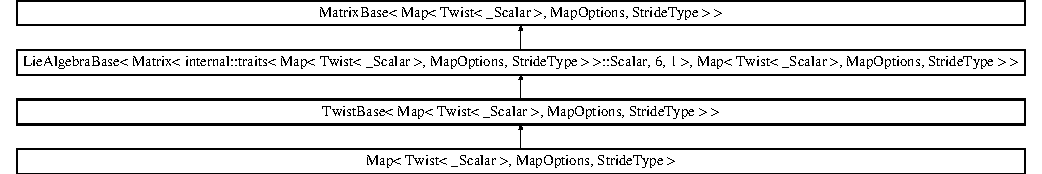
\includegraphics[height=2.333333cm]{class_map_3_01_twist_3_01___scalar_01_4_00_01_map_options_00_01_stride_type_01_4}
\end{center}
\end{figure}
\subsection*{Public Types}
\begin{DoxyCompactItemize}
\item 
typedef internal\+::traits$<$ \hyperlink{class_map_3_01_twist_3_01___scalar_01_4_00_01_map_options_00_01_stride_type_01_4_a7bc49d9365cdda555f4d107d55a1c6b2}{Map} $>$\+::\hyperlink{class_map_3_01_twist_3_01___scalar_01_4_00_01_map_options_00_01_stride_type_01_4_aed5862495c86340dcb689412d79eb66a}{Coefficients} \hyperlink{class_map_3_01_twist_3_01___scalar_01_4_00_01_map_options_00_01_stride_type_01_4_aed5862495c86340dcb689412d79eb66a}{Coefficients}
\end{DoxyCompactItemize}
\subsection*{Public Member Functions}
\begin{DoxyCompactItemize}
\item 
\hyperlink{class_map_3_01_twist_3_01___scalar_01_4_00_01_map_options_00_01_stride_type_01_4_a7bc49d9365cdda555f4d107d55a1c6b2}{Map} (const \hyperlink{class_twist}{Twist}$<$ Scalar $>$ \&d)
\item 
{\footnotesize template$<$int \+\_\+\+Rows, int \+\_\+\+Cols, int \+\_\+\+Options, int \+\_\+\+Max\+Rows, int \+\_\+\+Max\+Cols$>$ }\\\hyperlink{class_map_3_01_twist_3_01___scalar_01_4_00_01_map_options_00_01_stride_type_01_4_a469bc8175fab999f31a1c38c88fdd47b}{Map} (const Array$<$ Scalar, \+\_\+\+Rows, \+\_\+\+Cols, \+\_\+\+Options, \+\_\+\+Max\+Rows, \+\_\+\+Max\+Cols $>$ \&g)
\item 
\hyperlink{class_map_3_01_twist_3_01___scalar_01_4_00_01_map_options_00_01_stride_type_01_4_a7bd37d5ef0abea2b92aaae685fd38e69}{Map} (Scalar $\ast$data)
\item 
\hyperlink{class_map_3_01_twist_3_01___scalar_01_4_00_01_map_options_00_01_stride_type_01_4_a8f9f7e5bc9955feeebb7b9bc5fb783be}{Map} (const Map \&m)
\item 
\hyperlink{class_map_3_01_twist_3_01___scalar_01_4_00_01_map_options_00_01_stride_type_01_4_aed5862495c86340dcb689412d79eb66a}{Coefficients} \& \hyperlink{class_map_3_01_twist_3_01___scalar_01_4_00_01_map_options_00_01_stride_type_01_4_a53ade1199e68bed6af76d750b17a86b1}{get} ()
\item 
const \hyperlink{class_map_3_01_twist_3_01___scalar_01_4_00_01_map_options_00_01_stride_type_01_4_aed5862495c86340dcb689412d79eb66a}{Coefficients} \& \hyperlink{class_map_3_01_twist_3_01___scalar_01_4_00_01_map_options_00_01_stride_type_01_4_a6d725b7694668b1cd73c37cd6e1794ef}{get} () const
\end{DoxyCompactItemize}
\subsection*{Protected Types}
\begin{DoxyCompactItemize}
\item 
typedef \hyperlink{class_twist_base}{Twist\+Base}$<$ \hyperlink{class_map_3_01_twist_3_01___scalar_01_4_00_01_map_options_00_01_stride_type_01_4_a7bc49d9365cdda555f4d107d55a1c6b2}{Map}$<$ \hyperlink{class_twist}{Twist}$<$ \+\_\+\+Scalar $>$ $>$ $>$ \hyperlink{class_map_3_01_twist_3_01___scalar_01_4_00_01_map_options_00_01_stride_type_01_4_a1d92d7e062d98f16684181244775ea6c}{Base}
\end{DoxyCompactItemize}
\subsection*{Protected Attributes}
\begin{DoxyCompactItemize}
\item 
\hyperlink{class_map_3_01_twist_3_01___scalar_01_4_00_01_map_options_00_01_stride_type_01_4_aed5862495c86340dcb689412d79eb66a}{Coefficients} \hyperlink{class_map_3_01_twist_3_01___scalar_01_4_00_01_map_options_00_01_stride_type_01_4_a393cb065b2aa091a7a5b5c66eca9861a}{m\+\_\+coeffs}
\end{DoxyCompactItemize}


\subsection{Detailed Description}
\subsubsection*{template$<$typename \+\_\+\+Scalar, int Map\+Options, typename Stride\+Type$>$\newline
class Map$<$ Twist$<$ \+\_\+\+Scalar $>$, Map\+Options, Stride\+Type $>$}

Class map an array to twist. 


\begin{DoxyTemplParams}{Template Parameters}
{\em \+\_\+\+Scalar} & the type of the underlying array \\
\hline
{\em Map\+Options} & \\
\hline
\end{DoxyTemplParams}
\begin{DoxySeeAlso}{See also}
\hyperlink{class_map_3_01_twist_3_01___scalar_01_4_00_01_map_options_00_01_stride_type_01_4_a7bc49d9365cdda555f4d107d55a1c6b2}{Map$<$\+Matrix$>$} 
\end{DoxySeeAlso}

\begin{DoxyTemplParams}{Template Parameters}
{\em Stride\+Type} & \\
\hline
\end{DoxyTemplParams}
\begin{DoxySeeAlso}{See also}
\hyperlink{class_map_3_01_twist_3_01___scalar_01_4_00_01_map_options_00_01_stride_type_01_4_a7bc49d9365cdda555f4d107d55a1c6b2}{Map$<$\+Matrix$>$}

The methods are defined in \hyperlink{class_lie_algebra_base}{Lie\+Algebra\+Base} and \hyperlink{class_twist_base}{Twist\+Base} 
\end{DoxySeeAlso}


Definition at line 227 of file Twist.\+h.



\subsection{Member Typedef Documentation}
\hypertarget{class_map_3_01_twist_3_01___scalar_01_4_00_01_map_options_00_01_stride_type_01_4_a1d92d7e062d98f16684181244775ea6c}{}\label{class_map_3_01_twist_3_01___scalar_01_4_00_01_map_options_00_01_stride_type_01_4_a1d92d7e062d98f16684181244775ea6c} 
\index{Map$<$ Twist$<$ \+\_\+\+Scalar $>$, Map\+Options, Stride\+Type $>$@{Map$<$ Twist$<$ \+\_\+\+Scalar $>$, Map\+Options, Stride\+Type $>$}!Base@{Base}}
\index{Base@{Base}!Map$<$ Twist$<$ \+\_\+\+Scalar $>$, Map\+Options, Stride\+Type $>$@{Map$<$ Twist$<$ \+\_\+\+Scalar $>$, Map\+Options, Stride\+Type $>$}}
\subsubsection{\texorpdfstring{Base}{Base}}
{\footnotesize\ttfamily template$<$typename \+\_\+\+Scalar , int Map\+Options, typename Stride\+Type $>$ \\
typedef \hyperlink{class_twist_base}{Twist\+Base}$<$\hyperlink{class_map_3_01_twist_3_01___scalar_01_4_00_01_map_options_00_01_stride_type_01_4_a7bc49d9365cdda555f4d107d55a1c6b2}{Map}$<$\hyperlink{class_twist}{Twist}$<$\+\_\+\+Scalar$>$ $>$ $>$ \hyperlink{class_map_3_01_twist_3_01___scalar_01_4_00_01_map_options_00_01_stride_type_01_4_a7bc49d9365cdda555f4d107d55a1c6b2}{Map}$<$ \hyperlink{class_twist}{Twist}$<$ \+\_\+\+Scalar $>$, Map\+Options, Stride\+Type $>$\+::\hyperlink{class_map_3_01_twist_3_01___scalar_01_4_00_01_map_options_00_01_stride_type_01_4_a1d92d7e062d98f16684181244775ea6c}{Base}\hspace{0.3cm}{\ttfamily [protected]}}



Definition at line 229 of file Twist.\+h.

\hypertarget{class_map_3_01_twist_3_01___scalar_01_4_00_01_map_options_00_01_stride_type_01_4_aed5862495c86340dcb689412d79eb66a}{}\label{class_map_3_01_twist_3_01___scalar_01_4_00_01_map_options_00_01_stride_type_01_4_aed5862495c86340dcb689412d79eb66a} 
\index{Map$<$ Twist$<$ \+\_\+\+Scalar $>$, Map\+Options, Stride\+Type $>$@{Map$<$ Twist$<$ \+\_\+\+Scalar $>$, Map\+Options, Stride\+Type $>$}!Coefficients@{Coefficients}}
\index{Coefficients@{Coefficients}!Map$<$ Twist$<$ \+\_\+\+Scalar $>$, Map\+Options, Stride\+Type $>$@{Map$<$ Twist$<$ \+\_\+\+Scalar $>$, Map\+Options, Stride\+Type $>$}}
\subsubsection{\texorpdfstring{Coefficients}{Coefficients}}
{\footnotesize\ttfamily template$<$typename \+\_\+\+Scalar , int Map\+Options, typename Stride\+Type $>$ \\
typedef internal\+::traits$<$\hyperlink{class_map_3_01_twist_3_01___scalar_01_4_00_01_map_options_00_01_stride_type_01_4_a7bc49d9365cdda555f4d107d55a1c6b2}{Map}$>$\+::\hyperlink{class_map_3_01_twist_3_01___scalar_01_4_00_01_map_options_00_01_stride_type_01_4_aed5862495c86340dcb689412d79eb66a}{Coefficients} \hyperlink{class_map_3_01_twist_3_01___scalar_01_4_00_01_map_options_00_01_stride_type_01_4_a7bc49d9365cdda555f4d107d55a1c6b2}{Map}$<$ \hyperlink{class_twist}{Twist}$<$ \+\_\+\+Scalar $>$, Map\+Options, Stride\+Type $>$\+::\hyperlink{class_map_3_01_twist_3_01___scalar_01_4_00_01_map_options_00_01_stride_type_01_4_aed5862495c86340dcb689412d79eb66a}{Coefficients}}



Definition at line 233 of file Twist.\+h.



\subsection{Constructor \& Destructor Documentation}
\hypertarget{class_map_3_01_twist_3_01___scalar_01_4_00_01_map_options_00_01_stride_type_01_4_a7bc49d9365cdda555f4d107d55a1c6b2}{}\label{class_map_3_01_twist_3_01___scalar_01_4_00_01_map_options_00_01_stride_type_01_4_a7bc49d9365cdda555f4d107d55a1c6b2} 
\index{Map$<$ Twist$<$ \+\_\+\+Scalar $>$, Map\+Options, Stride\+Type $>$@{Map$<$ Twist$<$ \+\_\+\+Scalar $>$, Map\+Options, Stride\+Type $>$}!Map@{Map}}
\index{Map@{Map}!Map$<$ Twist$<$ \+\_\+\+Scalar $>$, Map\+Options, Stride\+Type $>$@{Map$<$ Twist$<$ \+\_\+\+Scalar $>$, Map\+Options, Stride\+Type $>$}}
\subsubsection{\texorpdfstring{Map()}{Map()}\hspace{0.1cm}{\footnotesize\ttfamily [1/4]}}
{\footnotesize\ttfamily template$<$typename \+\_\+\+Scalar , int Map\+Options, typename Stride\+Type $>$ \\
Map$<$ \hyperlink{class_twist}{Twist}$<$ \+\_\+\+Scalar $>$, Map\+Options, Stride\+Type $>$\+::Map (\begin{DoxyParamCaption}\item[{const \hyperlink{class_twist}{Twist}$<$ Scalar $>$ \&}]{d }\end{DoxyParamCaption})\hspace{0.3cm}{\ttfamily [inline]}}



Definition at line 235 of file Twist.\+h.

\hypertarget{class_map_3_01_twist_3_01___scalar_01_4_00_01_map_options_00_01_stride_type_01_4_a469bc8175fab999f31a1c38c88fdd47b}{}\label{class_map_3_01_twist_3_01___scalar_01_4_00_01_map_options_00_01_stride_type_01_4_a469bc8175fab999f31a1c38c88fdd47b} 
\index{Map$<$ Twist$<$ \+\_\+\+Scalar $>$, Map\+Options, Stride\+Type $>$@{Map$<$ Twist$<$ \+\_\+\+Scalar $>$, Map\+Options, Stride\+Type $>$}!Map@{Map}}
\index{Map@{Map}!Map$<$ Twist$<$ \+\_\+\+Scalar $>$, Map\+Options, Stride\+Type $>$@{Map$<$ Twist$<$ \+\_\+\+Scalar $>$, Map\+Options, Stride\+Type $>$}}
\subsubsection{\texorpdfstring{Map()}{Map()}\hspace{0.1cm}{\footnotesize\ttfamily [2/4]}}
{\footnotesize\ttfamily template$<$typename \+\_\+\+Scalar , int Map\+Options, typename Stride\+Type $>$ \\
template$<$int \+\_\+\+Rows, int \+\_\+\+Cols, int \+\_\+\+Options, int \+\_\+\+Max\+Rows, int \+\_\+\+Max\+Cols$>$ \\
Map$<$ \hyperlink{class_twist}{Twist}$<$ \+\_\+\+Scalar $>$, Map\+Options, Stride\+Type $>$\+::Map (\begin{DoxyParamCaption}\item[{const Array$<$ Scalar, \+\_\+\+Rows, \+\_\+\+Cols, \+\_\+\+Options, \+\_\+\+Max\+Rows, \+\_\+\+Max\+Cols $>$ \&}]{g }\end{DoxyParamCaption})\hspace{0.3cm}{\ttfamily [inline]}}



Definition at line 237 of file Twist.\+h.

\hypertarget{class_map_3_01_twist_3_01___scalar_01_4_00_01_map_options_00_01_stride_type_01_4_a7bd37d5ef0abea2b92aaae685fd38e69}{}\label{class_map_3_01_twist_3_01___scalar_01_4_00_01_map_options_00_01_stride_type_01_4_a7bd37d5ef0abea2b92aaae685fd38e69} 
\index{Map$<$ Twist$<$ \+\_\+\+Scalar $>$, Map\+Options, Stride\+Type $>$@{Map$<$ Twist$<$ \+\_\+\+Scalar $>$, Map\+Options, Stride\+Type $>$}!Map@{Map}}
\index{Map@{Map}!Map$<$ Twist$<$ \+\_\+\+Scalar $>$, Map\+Options, Stride\+Type $>$@{Map$<$ Twist$<$ \+\_\+\+Scalar $>$, Map\+Options, Stride\+Type $>$}}
\subsubsection{\texorpdfstring{Map()}{Map()}\hspace{0.1cm}{\footnotesize\ttfamily [3/4]}}
{\footnotesize\ttfamily template$<$typename \+\_\+\+Scalar , int Map\+Options, typename Stride\+Type $>$ \\
Map$<$ \hyperlink{class_twist}{Twist}$<$ \+\_\+\+Scalar $>$, Map\+Options, Stride\+Type $>$\+::Map (\begin{DoxyParamCaption}\item[{Scalar $\ast$}]{data }\end{DoxyParamCaption})\hspace{0.3cm}{\ttfamily [inline]}}



Definition at line 239 of file Twist.\+h.

\hypertarget{class_map_3_01_twist_3_01___scalar_01_4_00_01_map_options_00_01_stride_type_01_4_a8f9f7e5bc9955feeebb7b9bc5fb783be}{}\label{class_map_3_01_twist_3_01___scalar_01_4_00_01_map_options_00_01_stride_type_01_4_a8f9f7e5bc9955feeebb7b9bc5fb783be} 
\index{Map$<$ Twist$<$ \+\_\+\+Scalar $>$, Map\+Options, Stride\+Type $>$@{Map$<$ Twist$<$ \+\_\+\+Scalar $>$, Map\+Options, Stride\+Type $>$}!Map@{Map}}
\index{Map@{Map}!Map$<$ Twist$<$ \+\_\+\+Scalar $>$, Map\+Options, Stride\+Type $>$@{Map$<$ Twist$<$ \+\_\+\+Scalar $>$, Map\+Options, Stride\+Type $>$}}
\subsubsection{\texorpdfstring{Map()}{Map()}\hspace{0.1cm}{\footnotesize\ttfamily [4/4]}}
{\footnotesize\ttfamily template$<$typename \+\_\+\+Scalar , int Map\+Options, typename Stride\+Type $>$ \\
Map$<$ \hyperlink{class_twist}{Twist}$<$ \+\_\+\+Scalar $>$, Map\+Options, Stride\+Type $>$\+::Map (\begin{DoxyParamCaption}\item[{const Map$<$ \hyperlink{class_twist}{Twist}$<$ \+\_\+\+Scalar $>$, Map\+Options, Stride\+Type $>$ \&}]{m }\end{DoxyParamCaption})\hspace{0.3cm}{\ttfamily [inline]}}



Definition at line 240 of file Twist.\+h.



\subsection{Member Function Documentation}
\hypertarget{class_map_3_01_twist_3_01___scalar_01_4_00_01_map_options_00_01_stride_type_01_4_a53ade1199e68bed6af76d750b17a86b1}{}\label{class_map_3_01_twist_3_01___scalar_01_4_00_01_map_options_00_01_stride_type_01_4_a53ade1199e68bed6af76d750b17a86b1} 
\index{Map$<$ Twist$<$ \+\_\+\+Scalar $>$, Map\+Options, Stride\+Type $>$@{Map$<$ Twist$<$ \+\_\+\+Scalar $>$, Map\+Options, Stride\+Type $>$}!get@{get}}
\index{get@{get}!Map$<$ Twist$<$ \+\_\+\+Scalar $>$, Map\+Options, Stride\+Type $>$@{Map$<$ Twist$<$ \+\_\+\+Scalar $>$, Map\+Options, Stride\+Type $>$}}
\subsubsection{\texorpdfstring{get()}{get()}\hspace{0.1cm}{\footnotesize\ttfamily [1/2]}}
{\footnotesize\ttfamily template$<$typename \+\_\+\+Scalar , int Map\+Options, typename Stride\+Type $>$ \\
\hyperlink{class_map_3_01_twist_3_01___scalar_01_4_00_01_map_options_00_01_stride_type_01_4_aed5862495c86340dcb689412d79eb66a}{Coefficients}\& \hyperlink{class_map_3_01_twist_3_01___scalar_01_4_00_01_map_options_00_01_stride_type_01_4_a7bc49d9365cdda555f4d107d55a1c6b2}{Map}$<$ \hyperlink{class_twist}{Twist}$<$ \+\_\+\+Scalar $>$, Map\+Options, Stride\+Type $>$\+::get (\begin{DoxyParamCaption}{ }\end{DoxyParamCaption})\hspace{0.3cm}{\ttfamily [inline]}}



Definition at line 242 of file Twist.\+h.

\hypertarget{class_map_3_01_twist_3_01___scalar_01_4_00_01_map_options_00_01_stride_type_01_4_a6d725b7694668b1cd73c37cd6e1794ef}{}\label{class_map_3_01_twist_3_01___scalar_01_4_00_01_map_options_00_01_stride_type_01_4_a6d725b7694668b1cd73c37cd6e1794ef} 
\index{Map$<$ Twist$<$ \+\_\+\+Scalar $>$, Map\+Options, Stride\+Type $>$@{Map$<$ Twist$<$ \+\_\+\+Scalar $>$, Map\+Options, Stride\+Type $>$}!get@{get}}
\index{get@{get}!Map$<$ Twist$<$ \+\_\+\+Scalar $>$, Map\+Options, Stride\+Type $>$@{Map$<$ Twist$<$ \+\_\+\+Scalar $>$, Map\+Options, Stride\+Type $>$}}
\subsubsection{\texorpdfstring{get()}{get()}\hspace{0.1cm}{\footnotesize\ttfamily [2/2]}}
{\footnotesize\ttfamily template$<$typename \+\_\+\+Scalar , int Map\+Options, typename Stride\+Type $>$ \\
const \hyperlink{class_map_3_01_twist_3_01___scalar_01_4_00_01_map_options_00_01_stride_type_01_4_aed5862495c86340dcb689412d79eb66a}{Coefficients}\& \hyperlink{class_map_3_01_twist_3_01___scalar_01_4_00_01_map_options_00_01_stride_type_01_4_a7bc49d9365cdda555f4d107d55a1c6b2}{Map}$<$ \hyperlink{class_twist}{Twist}$<$ \+\_\+\+Scalar $>$, Map\+Options, Stride\+Type $>$\+::get (\begin{DoxyParamCaption}{ }\end{DoxyParamCaption}) const\hspace{0.3cm}{\ttfamily [inline]}}



Definition at line 243 of file Twist.\+h.



\subsection{Member Data Documentation}
\hypertarget{class_map_3_01_twist_3_01___scalar_01_4_00_01_map_options_00_01_stride_type_01_4_a393cb065b2aa091a7a5b5c66eca9861a}{}\label{class_map_3_01_twist_3_01___scalar_01_4_00_01_map_options_00_01_stride_type_01_4_a393cb065b2aa091a7a5b5c66eca9861a} 
\index{Map$<$ Twist$<$ \+\_\+\+Scalar $>$, Map\+Options, Stride\+Type $>$@{Map$<$ Twist$<$ \+\_\+\+Scalar $>$, Map\+Options, Stride\+Type $>$}!m\+\_\+coeffs@{m\+\_\+coeffs}}
\index{m\+\_\+coeffs@{m\+\_\+coeffs}!Map$<$ Twist$<$ \+\_\+\+Scalar $>$, Map\+Options, Stride\+Type $>$@{Map$<$ Twist$<$ \+\_\+\+Scalar $>$, Map\+Options, Stride\+Type $>$}}
\subsubsection{\texorpdfstring{m\+\_\+coeffs}{m\_coeffs}}
{\footnotesize\ttfamily template$<$typename \+\_\+\+Scalar , int Map\+Options, typename Stride\+Type $>$ \\
\hyperlink{class_map_3_01_twist_3_01___scalar_01_4_00_01_map_options_00_01_stride_type_01_4_aed5862495c86340dcb689412d79eb66a}{Coefficients} \hyperlink{class_map_3_01_twist_3_01___scalar_01_4_00_01_map_options_00_01_stride_type_01_4_a7bc49d9365cdda555f4d107d55a1c6b2}{Map}$<$ \hyperlink{class_twist}{Twist}$<$ \+\_\+\+Scalar $>$, Map\+Options, Stride\+Type $>$\+::m\+\_\+coeffs\hspace{0.3cm}{\ttfamily [protected]}}



Definition at line 246 of file Twist.\+h.



The documentation for this class was generated from the following file\+:\begin{DoxyCompactItemize}
\item 
/\+Users/\+Ryan/\+Code/codyco-\/superbuild/libraries/\+Eigen\+Lgsm/unsupported/\+Eigen/src/\+Lgsm/\hyperlink{_twist_8h}{Twist.\+h}\end{DoxyCompactItemize}

\hypertarget{class_map_3_01_wrench_3_01___scalar_01_4_00_01_map_options_00_01_stride_type_01_4}{}\section{Map$<$ Wrench$<$ \+\_\+\+Scalar $>$, Map\+Options, Stride\+Type $>$ Class Template Reference}
\label{class_map_3_01_wrench_3_01___scalar_01_4_00_01_map_options_00_01_stride_type_01_4}\index{Map$<$ Wrench$<$ \+\_\+\+Scalar $>$, Map\+Options, Stride\+Type $>$@{Map$<$ Wrench$<$ \+\_\+\+Scalar $>$, Map\+Options, Stride\+Type $>$}}


Class map an array to wrench.  




{\ttfamily \#include $<$Wrench.\+h$>$}

Inheritance diagram for Map$<$ Wrench$<$ \+\_\+\+Scalar $>$, Map\+Options, Stride\+Type $>$\+:\begin{figure}[H]
\begin{center}
\leavevmode
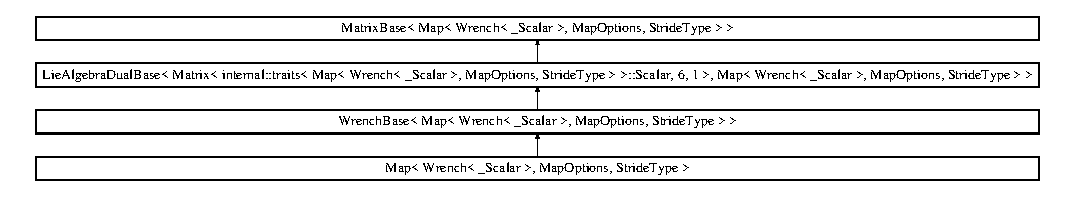
\includegraphics[height=2.200393cm]{class_map_3_01_wrench_3_01___scalar_01_4_00_01_map_options_00_01_stride_type_01_4}
\end{center}
\end{figure}
\subsection*{Public Types}
\begin{DoxyCompactItemize}
\item 
typedef internal\+::traits$<$ \hyperlink{class_map_3_01_wrench_3_01___scalar_01_4_00_01_map_options_00_01_stride_type_01_4_ab778c7158f5d29d76672346ecfe4e3ea}{Map} $>$\+::\hyperlink{class_map_3_01_wrench_3_01___scalar_01_4_00_01_map_options_00_01_stride_type_01_4_abfc1bf3f7dc1d3051325edad634172e8}{Coefficients} \hyperlink{class_map_3_01_wrench_3_01___scalar_01_4_00_01_map_options_00_01_stride_type_01_4_abfc1bf3f7dc1d3051325edad634172e8}{Coefficients}
\end{DoxyCompactItemize}
\subsection*{Public Member Functions}
\begin{DoxyCompactItemize}
\item 
\hyperlink{class_map_3_01_wrench_3_01___scalar_01_4_00_01_map_options_00_01_stride_type_01_4_ab778c7158f5d29d76672346ecfe4e3ea}{Map} (const \hyperlink{class_wrench}{Wrench}$<$ Scalar $>$ \&w)
\item 
{\footnotesize template$<$int \+\_\+\+Rows, int \+\_\+\+Cols, int \+\_\+\+Options, int \+\_\+\+Max\+Rows, int \+\_\+\+Max\+Cols$>$ }\\\hyperlink{class_map_3_01_wrench_3_01___scalar_01_4_00_01_map_options_00_01_stride_type_01_4_a3691be9d7061572f33fec65663c620a5}{Map} (const Array$<$ Scalar, \+\_\+\+Rows, \+\_\+\+Cols, \+\_\+\+Options, \+\_\+\+Max\+Rows, \+\_\+\+Max\+Cols $>$ \&g)
\item 
\hyperlink{class_map_3_01_wrench_3_01___scalar_01_4_00_01_map_options_00_01_stride_type_01_4_a64c75a02aa57da4b0d5fdeda620912e1}{Map} (Scalar $\ast$data)
\item 
\hyperlink{class_map_3_01_wrench_3_01___scalar_01_4_00_01_map_options_00_01_stride_type_01_4_a4f2480bbfd79778a5feb90f8beb30601}{Map} (const Map \&m)
\item 
\hyperlink{class_map_3_01_wrench_3_01___scalar_01_4_00_01_map_options_00_01_stride_type_01_4_abfc1bf3f7dc1d3051325edad634172e8}{Coefficients} \& \hyperlink{class_map_3_01_wrench_3_01___scalar_01_4_00_01_map_options_00_01_stride_type_01_4_ac2661fbf02f8a1009057aee6667b3d95}{get} ()
\item 
const \hyperlink{class_map_3_01_wrench_3_01___scalar_01_4_00_01_map_options_00_01_stride_type_01_4_abfc1bf3f7dc1d3051325edad634172e8}{Coefficients} \& \hyperlink{class_map_3_01_wrench_3_01___scalar_01_4_00_01_map_options_00_01_stride_type_01_4_ab25730235675b6ac5e04b222931a5050}{get} () const
\end{DoxyCompactItemize}
\subsection*{Protected Types}
\begin{DoxyCompactItemize}
\item 
typedef \hyperlink{class_wrench_base}{Wrench\+Base}$<$ \hyperlink{class_map_3_01_wrench_3_01___scalar_01_4_00_01_map_options_00_01_stride_type_01_4_ab778c7158f5d29d76672346ecfe4e3ea}{Map}$<$ \hyperlink{class_wrench}{Wrench}$<$ \+\_\+\+Scalar $>$ $>$ $>$ \hyperlink{class_map_3_01_wrench_3_01___scalar_01_4_00_01_map_options_00_01_stride_type_01_4_ae2acfdad9b8a19976e088f86e664d657}{Base}
\end{DoxyCompactItemize}
\subsection*{Protected Attributes}
\begin{DoxyCompactItemize}
\item 
\hyperlink{class_map_3_01_wrench_3_01___scalar_01_4_00_01_map_options_00_01_stride_type_01_4_abfc1bf3f7dc1d3051325edad634172e8}{Coefficients} \hyperlink{class_map_3_01_wrench_3_01___scalar_01_4_00_01_map_options_00_01_stride_type_01_4_a77801912f5f6b222ed126ed4002a8edf}{m\+\_\+coeffs}
\end{DoxyCompactItemize}


\subsection{Detailed Description}
\subsubsection*{template$<$typename \+\_\+\+Scalar, int Map\+Options, typename Stride\+Type$>$\newline
class Map$<$ Wrench$<$ \+\_\+\+Scalar $>$, Map\+Options, Stride\+Type $>$}

Class map an array to wrench. 


\begin{DoxyTemplParams}{Template Parameters}
{\em \+\_\+\+Scalar} & the type of the underlying array \\
\hline
{\em Map\+Options} & \\
\hline
\end{DoxyTemplParams}
\begin{DoxySeeAlso}{See also}
\hyperlink{class_map_3_01_wrench_3_01___scalar_01_4_00_01_map_options_00_01_stride_type_01_4_ab778c7158f5d29d76672346ecfe4e3ea}{Map$<$\+Matrix$>$} 
\end{DoxySeeAlso}

\begin{DoxyTemplParams}{Template Parameters}
{\em Stride\+Type} & \\
\hline
\end{DoxyTemplParams}
\begin{DoxySeeAlso}{See also}
\hyperlink{class_map_3_01_wrench_3_01___scalar_01_4_00_01_map_options_00_01_stride_type_01_4_ab778c7158f5d29d76672346ecfe4e3ea}{Map$<$\+Matrix$>$}

The methods are defined in \hyperlink{class_lie_algebra_base}{Lie\+Algebra\+Base} and \hyperlink{class_wrench_base}{Wrench\+Base} 
\end{DoxySeeAlso}


Definition at line 217 of file Wrench.\+h.



\subsection{Member Typedef Documentation}
\hypertarget{class_map_3_01_wrench_3_01___scalar_01_4_00_01_map_options_00_01_stride_type_01_4_ae2acfdad9b8a19976e088f86e664d657}{}\label{class_map_3_01_wrench_3_01___scalar_01_4_00_01_map_options_00_01_stride_type_01_4_ae2acfdad9b8a19976e088f86e664d657} 
\index{Map$<$ Wrench$<$ \+\_\+\+Scalar $>$, Map\+Options, Stride\+Type $>$@{Map$<$ Wrench$<$ \+\_\+\+Scalar $>$, Map\+Options, Stride\+Type $>$}!Base@{Base}}
\index{Base@{Base}!Map$<$ Wrench$<$ \+\_\+\+Scalar $>$, Map\+Options, Stride\+Type $>$@{Map$<$ Wrench$<$ \+\_\+\+Scalar $>$, Map\+Options, Stride\+Type $>$}}
\subsubsection{\texorpdfstring{Base}{Base}}
{\footnotesize\ttfamily template$<$typename \+\_\+\+Scalar , int Map\+Options, typename Stride\+Type $>$ \\
typedef \hyperlink{class_wrench_base}{Wrench\+Base}$<$\hyperlink{class_map_3_01_wrench_3_01___scalar_01_4_00_01_map_options_00_01_stride_type_01_4_ab778c7158f5d29d76672346ecfe4e3ea}{Map}$<$\hyperlink{class_wrench}{Wrench}$<$\+\_\+\+Scalar$>$ $>$ $>$ \hyperlink{class_map_3_01_wrench_3_01___scalar_01_4_00_01_map_options_00_01_stride_type_01_4_ab778c7158f5d29d76672346ecfe4e3ea}{Map}$<$ \hyperlink{class_wrench}{Wrench}$<$ \+\_\+\+Scalar $>$, Map\+Options, Stride\+Type $>$\+::\hyperlink{class_map_3_01_wrench_3_01___scalar_01_4_00_01_map_options_00_01_stride_type_01_4_ae2acfdad9b8a19976e088f86e664d657}{Base}\hspace{0.3cm}{\ttfamily [protected]}}



Definition at line 219 of file Wrench.\+h.

\hypertarget{class_map_3_01_wrench_3_01___scalar_01_4_00_01_map_options_00_01_stride_type_01_4_abfc1bf3f7dc1d3051325edad634172e8}{}\label{class_map_3_01_wrench_3_01___scalar_01_4_00_01_map_options_00_01_stride_type_01_4_abfc1bf3f7dc1d3051325edad634172e8} 
\index{Map$<$ Wrench$<$ \+\_\+\+Scalar $>$, Map\+Options, Stride\+Type $>$@{Map$<$ Wrench$<$ \+\_\+\+Scalar $>$, Map\+Options, Stride\+Type $>$}!Coefficients@{Coefficients}}
\index{Coefficients@{Coefficients}!Map$<$ Wrench$<$ \+\_\+\+Scalar $>$, Map\+Options, Stride\+Type $>$@{Map$<$ Wrench$<$ \+\_\+\+Scalar $>$, Map\+Options, Stride\+Type $>$}}
\subsubsection{\texorpdfstring{Coefficients}{Coefficients}}
{\footnotesize\ttfamily template$<$typename \+\_\+\+Scalar , int Map\+Options, typename Stride\+Type $>$ \\
typedef internal\+::traits$<$\hyperlink{class_map_3_01_wrench_3_01___scalar_01_4_00_01_map_options_00_01_stride_type_01_4_ab778c7158f5d29d76672346ecfe4e3ea}{Map}$>$\+::\hyperlink{class_map_3_01_wrench_3_01___scalar_01_4_00_01_map_options_00_01_stride_type_01_4_abfc1bf3f7dc1d3051325edad634172e8}{Coefficients} \hyperlink{class_map_3_01_wrench_3_01___scalar_01_4_00_01_map_options_00_01_stride_type_01_4_ab778c7158f5d29d76672346ecfe4e3ea}{Map}$<$ \hyperlink{class_wrench}{Wrench}$<$ \+\_\+\+Scalar $>$, Map\+Options, Stride\+Type $>$\+::\hyperlink{class_map_3_01_wrench_3_01___scalar_01_4_00_01_map_options_00_01_stride_type_01_4_abfc1bf3f7dc1d3051325edad634172e8}{Coefficients}}



Definition at line 224 of file Wrench.\+h.



\subsection{Constructor \& Destructor Documentation}
\hypertarget{class_map_3_01_wrench_3_01___scalar_01_4_00_01_map_options_00_01_stride_type_01_4_ab778c7158f5d29d76672346ecfe4e3ea}{}\label{class_map_3_01_wrench_3_01___scalar_01_4_00_01_map_options_00_01_stride_type_01_4_ab778c7158f5d29d76672346ecfe4e3ea} 
\index{Map$<$ Wrench$<$ \+\_\+\+Scalar $>$, Map\+Options, Stride\+Type $>$@{Map$<$ Wrench$<$ \+\_\+\+Scalar $>$, Map\+Options, Stride\+Type $>$}!Map@{Map}}
\index{Map@{Map}!Map$<$ Wrench$<$ \+\_\+\+Scalar $>$, Map\+Options, Stride\+Type $>$@{Map$<$ Wrench$<$ \+\_\+\+Scalar $>$, Map\+Options, Stride\+Type $>$}}
\subsubsection{\texorpdfstring{Map()}{Map()}\hspace{0.1cm}{\footnotesize\ttfamily [1/4]}}
{\footnotesize\ttfamily template$<$typename \+\_\+\+Scalar , int Map\+Options, typename Stride\+Type $>$ \\
Map$<$ \hyperlink{class_wrench}{Wrench}$<$ \+\_\+\+Scalar $>$, Map\+Options, Stride\+Type $>$\+::Map (\begin{DoxyParamCaption}\item[{const \hyperlink{class_wrench}{Wrench}$<$ Scalar $>$ \&}]{w }\end{DoxyParamCaption})\hspace{0.3cm}{\ttfamily [inline]}}



Definition at line 226 of file Wrench.\+h.

\hypertarget{class_map_3_01_wrench_3_01___scalar_01_4_00_01_map_options_00_01_stride_type_01_4_a3691be9d7061572f33fec65663c620a5}{}\label{class_map_3_01_wrench_3_01___scalar_01_4_00_01_map_options_00_01_stride_type_01_4_a3691be9d7061572f33fec65663c620a5} 
\index{Map$<$ Wrench$<$ \+\_\+\+Scalar $>$, Map\+Options, Stride\+Type $>$@{Map$<$ Wrench$<$ \+\_\+\+Scalar $>$, Map\+Options, Stride\+Type $>$}!Map@{Map}}
\index{Map@{Map}!Map$<$ Wrench$<$ \+\_\+\+Scalar $>$, Map\+Options, Stride\+Type $>$@{Map$<$ Wrench$<$ \+\_\+\+Scalar $>$, Map\+Options, Stride\+Type $>$}}
\subsubsection{\texorpdfstring{Map()}{Map()}\hspace{0.1cm}{\footnotesize\ttfamily [2/4]}}
{\footnotesize\ttfamily template$<$typename \+\_\+\+Scalar , int Map\+Options, typename Stride\+Type $>$ \\
template$<$int \+\_\+\+Rows, int \+\_\+\+Cols, int \+\_\+\+Options, int \+\_\+\+Max\+Rows, int \+\_\+\+Max\+Cols$>$ \\
Map$<$ \hyperlink{class_wrench}{Wrench}$<$ \+\_\+\+Scalar $>$, Map\+Options, Stride\+Type $>$\+::Map (\begin{DoxyParamCaption}\item[{const Array$<$ Scalar, \+\_\+\+Rows, \+\_\+\+Cols, \+\_\+\+Options, \+\_\+\+Max\+Rows, \+\_\+\+Max\+Cols $>$ \&}]{g }\end{DoxyParamCaption})\hspace{0.3cm}{\ttfamily [inline]}}



Definition at line 228 of file Wrench.\+h.

\hypertarget{class_map_3_01_wrench_3_01___scalar_01_4_00_01_map_options_00_01_stride_type_01_4_a64c75a02aa57da4b0d5fdeda620912e1}{}\label{class_map_3_01_wrench_3_01___scalar_01_4_00_01_map_options_00_01_stride_type_01_4_a64c75a02aa57da4b0d5fdeda620912e1} 
\index{Map$<$ Wrench$<$ \+\_\+\+Scalar $>$, Map\+Options, Stride\+Type $>$@{Map$<$ Wrench$<$ \+\_\+\+Scalar $>$, Map\+Options, Stride\+Type $>$}!Map@{Map}}
\index{Map@{Map}!Map$<$ Wrench$<$ \+\_\+\+Scalar $>$, Map\+Options, Stride\+Type $>$@{Map$<$ Wrench$<$ \+\_\+\+Scalar $>$, Map\+Options, Stride\+Type $>$}}
\subsubsection{\texorpdfstring{Map()}{Map()}\hspace{0.1cm}{\footnotesize\ttfamily [3/4]}}
{\footnotesize\ttfamily template$<$typename \+\_\+\+Scalar , int Map\+Options, typename Stride\+Type $>$ \\
Map$<$ \hyperlink{class_wrench}{Wrench}$<$ \+\_\+\+Scalar $>$, Map\+Options, Stride\+Type $>$\+::Map (\begin{DoxyParamCaption}\item[{Scalar $\ast$}]{data }\end{DoxyParamCaption})\hspace{0.3cm}{\ttfamily [inline]}}



Definition at line 230 of file Wrench.\+h.

\hypertarget{class_map_3_01_wrench_3_01___scalar_01_4_00_01_map_options_00_01_stride_type_01_4_a4f2480bbfd79778a5feb90f8beb30601}{}\label{class_map_3_01_wrench_3_01___scalar_01_4_00_01_map_options_00_01_stride_type_01_4_a4f2480bbfd79778a5feb90f8beb30601} 
\index{Map$<$ Wrench$<$ \+\_\+\+Scalar $>$, Map\+Options, Stride\+Type $>$@{Map$<$ Wrench$<$ \+\_\+\+Scalar $>$, Map\+Options, Stride\+Type $>$}!Map@{Map}}
\index{Map@{Map}!Map$<$ Wrench$<$ \+\_\+\+Scalar $>$, Map\+Options, Stride\+Type $>$@{Map$<$ Wrench$<$ \+\_\+\+Scalar $>$, Map\+Options, Stride\+Type $>$}}
\subsubsection{\texorpdfstring{Map()}{Map()}\hspace{0.1cm}{\footnotesize\ttfamily [4/4]}}
{\footnotesize\ttfamily template$<$typename \+\_\+\+Scalar , int Map\+Options, typename Stride\+Type $>$ \\
Map$<$ \hyperlink{class_wrench}{Wrench}$<$ \+\_\+\+Scalar $>$, Map\+Options, Stride\+Type $>$\+::Map (\begin{DoxyParamCaption}\item[{const Map$<$ \hyperlink{class_wrench}{Wrench}$<$ \+\_\+\+Scalar $>$, Map\+Options, Stride\+Type $>$ \&}]{m }\end{DoxyParamCaption})\hspace{0.3cm}{\ttfamily [inline]}}



Definition at line 231 of file Wrench.\+h.



\subsection{Member Function Documentation}
\hypertarget{class_map_3_01_wrench_3_01___scalar_01_4_00_01_map_options_00_01_stride_type_01_4_ac2661fbf02f8a1009057aee6667b3d95}{}\label{class_map_3_01_wrench_3_01___scalar_01_4_00_01_map_options_00_01_stride_type_01_4_ac2661fbf02f8a1009057aee6667b3d95} 
\index{Map$<$ Wrench$<$ \+\_\+\+Scalar $>$, Map\+Options, Stride\+Type $>$@{Map$<$ Wrench$<$ \+\_\+\+Scalar $>$, Map\+Options, Stride\+Type $>$}!get@{get}}
\index{get@{get}!Map$<$ Wrench$<$ \+\_\+\+Scalar $>$, Map\+Options, Stride\+Type $>$@{Map$<$ Wrench$<$ \+\_\+\+Scalar $>$, Map\+Options, Stride\+Type $>$}}
\subsubsection{\texorpdfstring{get()}{get()}\hspace{0.1cm}{\footnotesize\ttfamily [1/2]}}
{\footnotesize\ttfamily template$<$typename \+\_\+\+Scalar , int Map\+Options, typename Stride\+Type $>$ \\
\hyperlink{class_map_3_01_wrench_3_01___scalar_01_4_00_01_map_options_00_01_stride_type_01_4_abfc1bf3f7dc1d3051325edad634172e8}{Coefficients}\& \hyperlink{class_map_3_01_wrench_3_01___scalar_01_4_00_01_map_options_00_01_stride_type_01_4_ab778c7158f5d29d76672346ecfe4e3ea}{Map}$<$ \hyperlink{class_wrench}{Wrench}$<$ \+\_\+\+Scalar $>$, Map\+Options, Stride\+Type $>$\+::get (\begin{DoxyParamCaption}{ }\end{DoxyParamCaption})\hspace{0.3cm}{\ttfamily [inline]}}



Definition at line 233 of file Wrench.\+h.

\hypertarget{class_map_3_01_wrench_3_01___scalar_01_4_00_01_map_options_00_01_stride_type_01_4_ab25730235675b6ac5e04b222931a5050}{}\label{class_map_3_01_wrench_3_01___scalar_01_4_00_01_map_options_00_01_stride_type_01_4_ab25730235675b6ac5e04b222931a5050} 
\index{Map$<$ Wrench$<$ \+\_\+\+Scalar $>$, Map\+Options, Stride\+Type $>$@{Map$<$ Wrench$<$ \+\_\+\+Scalar $>$, Map\+Options, Stride\+Type $>$}!get@{get}}
\index{get@{get}!Map$<$ Wrench$<$ \+\_\+\+Scalar $>$, Map\+Options, Stride\+Type $>$@{Map$<$ Wrench$<$ \+\_\+\+Scalar $>$, Map\+Options, Stride\+Type $>$}}
\subsubsection{\texorpdfstring{get()}{get()}\hspace{0.1cm}{\footnotesize\ttfamily [2/2]}}
{\footnotesize\ttfamily template$<$typename \+\_\+\+Scalar , int Map\+Options, typename Stride\+Type $>$ \\
const \hyperlink{class_map_3_01_wrench_3_01___scalar_01_4_00_01_map_options_00_01_stride_type_01_4_abfc1bf3f7dc1d3051325edad634172e8}{Coefficients}\& \hyperlink{class_map_3_01_wrench_3_01___scalar_01_4_00_01_map_options_00_01_stride_type_01_4_ab778c7158f5d29d76672346ecfe4e3ea}{Map}$<$ \hyperlink{class_wrench}{Wrench}$<$ \+\_\+\+Scalar $>$, Map\+Options, Stride\+Type $>$\+::get (\begin{DoxyParamCaption}{ }\end{DoxyParamCaption}) const\hspace{0.3cm}{\ttfamily [inline]}}



Definition at line 234 of file Wrench.\+h.



\subsection{Member Data Documentation}
\hypertarget{class_map_3_01_wrench_3_01___scalar_01_4_00_01_map_options_00_01_stride_type_01_4_a77801912f5f6b222ed126ed4002a8edf}{}\label{class_map_3_01_wrench_3_01___scalar_01_4_00_01_map_options_00_01_stride_type_01_4_a77801912f5f6b222ed126ed4002a8edf} 
\index{Map$<$ Wrench$<$ \+\_\+\+Scalar $>$, Map\+Options, Stride\+Type $>$@{Map$<$ Wrench$<$ \+\_\+\+Scalar $>$, Map\+Options, Stride\+Type $>$}!m\+\_\+coeffs@{m\+\_\+coeffs}}
\index{m\+\_\+coeffs@{m\+\_\+coeffs}!Map$<$ Wrench$<$ \+\_\+\+Scalar $>$, Map\+Options, Stride\+Type $>$@{Map$<$ Wrench$<$ \+\_\+\+Scalar $>$, Map\+Options, Stride\+Type $>$}}
\subsubsection{\texorpdfstring{m\+\_\+coeffs}{m\_coeffs}}
{\footnotesize\ttfamily template$<$typename \+\_\+\+Scalar , int Map\+Options, typename Stride\+Type $>$ \\
\hyperlink{class_map_3_01_wrench_3_01___scalar_01_4_00_01_map_options_00_01_stride_type_01_4_abfc1bf3f7dc1d3051325edad634172e8}{Coefficients} \hyperlink{class_map_3_01_wrench_3_01___scalar_01_4_00_01_map_options_00_01_stride_type_01_4_ab778c7158f5d29d76672346ecfe4e3ea}{Map}$<$ \hyperlink{class_wrench}{Wrench}$<$ \+\_\+\+Scalar $>$, Map\+Options, Stride\+Type $>$\+::m\+\_\+coeffs\hspace{0.3cm}{\ttfamily [protected]}}



Definition at line 237 of file Wrench.\+h.



The documentation for this class was generated from the following file\+:\begin{DoxyCompactItemize}
\item 
/\+Users/\+Ryan/\+Code/codyco-\/superbuild/libraries/\+Eigen\+Lgsm/unsupported/\+Eigen/src/\+Lgsm/\hyperlink{_wrench_8h}{Wrench.\+h}\end{DoxyCompactItemize}

\hypertarget{class_s_e3_cubic_interpolator}{}\section{S\+E3\+Cubic\+Interpolator$<$ Scalar $>$ Class Template Reference}
\label{class_s_e3_cubic_interpolator}\index{S\+E3\+Cubic\+Interpolator$<$ Scalar $>$@{S\+E3\+Cubic\+Interpolator$<$ Scalar $>$}}


{\ttfamily \#include $<$S\+E3\+Cubic\+Interpolator.\+h$>$}

\subsection*{Public Types}
\begin{DoxyCompactItemize}
\item 
typedef std\+::vector$<$ \hyperlink{class_displacement}{Displacement}$<$ Scalar $>$, aligned\+\_\+allocator$<$ \hyperlink{class_displacement}{Displacement}$<$ Scalar $>$ $>$ $>$ \hyperlink{class_s_e3_cubic_interpolator_ad6c935ddaa217d370411c200321dc089}{Std\+Vector\+Displacement}
\item 
typedef std\+::vector$<$ \hyperlink{class_twist}{Twist}$<$ Scalar $>$, aligned\+\_\+allocator$<$ \hyperlink{class_twist}{Twist}$<$ Scalar $>$ $>$ $>$ \hyperlink{class_s_e3_cubic_interpolator_ae70acde9b57ec38aaf1eaeee50bb35c5}{Std\+Vector\+Twist}
\end{DoxyCompactItemize}
\subsection*{Public Member Functions}
\begin{DoxyCompactItemize}
\item 
\hyperlink{class_s_e3_cubic_interpolator_a17856cd852a2260ea88169617997b02e}{S\+E3\+Cubic\+Interpolator} ()
\item 
void \hyperlink{class_s_e3_cubic_interpolator_aa070ccd623a41b2eb12b6513aab14021}{set\+Control\+Point} (const \hyperlink{class_s_e3_cubic_interpolator_ad6c935ddaa217d370411c200321dc089}{Std\+Vector\+Displacement} \&control\+Points, const \hyperlink{class_s_e3_cubic_interpolator_ae70acde9b57ec38aaf1eaeee50bb35c5}{Std\+Vector\+Twist} \&control\+Velocities, const std\+::vector$<$ Scalar $>$ \&\hyperlink{class_s_e3_cubic_interpolator_ad8083c34a619f3cb55f35ccaffeb6154}{t})
\item 
void \hyperlink{class_s_e3_cubic_interpolator_aebb1a7f9c3123cd3df8cec6d9dc5a72a}{Interpolate} (\hyperlink{class_displacement}{Displacement}$<$ Scalar $>$ \&pos, \hyperlink{class_twist}{Twist}$<$ Scalar $>$ \&vel, const Scalar time) const
\end{DoxyCompactItemize}
\subsection*{Protected Attributes}
\begin{DoxyCompactItemize}
\item 
std\+::vector$<$ Scalar $>$ \hyperlink{class_s_e3_cubic_interpolator_ad8083c34a619f3cb55f35ccaffeb6154}{t}
\item 
\hyperlink{class_displacement}{Displacement}$<$ Scalar $>$ \hyperlink{class_s_e3_cubic_interpolator_a57ac720f2b715a74d29472dc9ba4e6f5}{H1}
\item 
\hyperlink{class_s_e3_cubic_interpolator_ae70acde9b57ec38aaf1eaeee50bb35c5}{Std\+Vector\+Twist} \hyperlink{class_s_e3_cubic_interpolator_ab1e8c4aa3aaef4fee220e7ef50f493c1}{ksi}
\item 
\hyperlink{class_s_e3_cubic_interpolator_ae70acde9b57ec38aaf1eaeee50bb35c5}{Std\+Vector\+Twist} \hyperlink{class_s_e3_cubic_interpolator_ad54c52fb731ed48fcebab82d2d6c1c57}{bi}
\item 
\hyperlink{class_s_e3_cubic_interpolator_ae70acde9b57ec38aaf1eaeee50bb35c5}{Std\+Vector\+Twist} \hyperlink{class_s_e3_cubic_interpolator_a45865a05f0ce3a10cfc69b992bee971e}{ci}
\item 
\hyperlink{class_s_e3_cubic_interpolator_ae70acde9b57ec38aaf1eaeee50bb35c5}{Std\+Vector\+Twist} \hyperlink{class_s_e3_cubic_interpolator_ac2edcd8d93807db3f241d49390a2e3dc}{di}
\item 
size\+\_\+t \hyperlink{class_s_e3_cubic_interpolator_a9294008dfdce440c453807ff4f6fee23}{n}
\end{DoxyCompactItemize}


\subsection{Detailed Description}
\subsubsection*{template$<$typename Scalar$>$\newline
class S\+E3\+Cubic\+Interpolator$<$ Scalar $>$}



Definition at line 22 of file S\+E3\+Cubic\+Interpolator.\+h.



\subsection{Member Typedef Documentation}
\hypertarget{class_s_e3_cubic_interpolator_ad6c935ddaa217d370411c200321dc089}{}\label{class_s_e3_cubic_interpolator_ad6c935ddaa217d370411c200321dc089} 
\index{S\+E3\+Cubic\+Interpolator@{S\+E3\+Cubic\+Interpolator}!Std\+Vector\+Displacement@{Std\+Vector\+Displacement}}
\index{Std\+Vector\+Displacement@{Std\+Vector\+Displacement}!S\+E3\+Cubic\+Interpolator@{S\+E3\+Cubic\+Interpolator}}
\subsubsection{\texorpdfstring{Std\+Vector\+Displacement}{StdVectorDisplacement}}
{\footnotesize\ttfamily template$<$typename Scalar $>$ \\
typedef std\+::vector$<$\hyperlink{class_displacement}{Displacement}$<$Scalar$>$, aligned\+\_\+allocator$<$\hyperlink{class_displacement}{Displacement}$<$Scalar$>$ $>$ $>$ \hyperlink{class_s_e3_cubic_interpolator}{S\+E3\+Cubic\+Interpolator}$<$ Scalar $>$\+::\hyperlink{class_s_e3_cubic_interpolator_ad6c935ddaa217d370411c200321dc089}{Std\+Vector\+Displacement}}



Definition at line 24 of file S\+E3\+Cubic\+Interpolator.\+h.

\hypertarget{class_s_e3_cubic_interpolator_ae70acde9b57ec38aaf1eaeee50bb35c5}{}\label{class_s_e3_cubic_interpolator_ae70acde9b57ec38aaf1eaeee50bb35c5} 
\index{S\+E3\+Cubic\+Interpolator@{S\+E3\+Cubic\+Interpolator}!Std\+Vector\+Twist@{Std\+Vector\+Twist}}
\index{Std\+Vector\+Twist@{Std\+Vector\+Twist}!S\+E3\+Cubic\+Interpolator@{S\+E3\+Cubic\+Interpolator}}
\subsubsection{\texorpdfstring{Std\+Vector\+Twist}{StdVectorTwist}}
{\footnotesize\ttfamily template$<$typename Scalar $>$ \\
typedef std\+::vector$<$\hyperlink{class_twist}{Twist}$<$Scalar$>$, aligned\+\_\+allocator$<$\hyperlink{class_twist}{Twist}$<$Scalar$>$ $>$ $>$ \hyperlink{class_s_e3_cubic_interpolator}{S\+E3\+Cubic\+Interpolator}$<$ Scalar $>$\+::\hyperlink{class_s_e3_cubic_interpolator_ae70acde9b57ec38aaf1eaeee50bb35c5}{Std\+Vector\+Twist}}



Definition at line 25 of file S\+E3\+Cubic\+Interpolator.\+h.



\subsection{Constructor \& Destructor Documentation}
\hypertarget{class_s_e3_cubic_interpolator_a17856cd852a2260ea88169617997b02e}{}\label{class_s_e3_cubic_interpolator_a17856cd852a2260ea88169617997b02e} 
\index{S\+E3\+Cubic\+Interpolator@{S\+E3\+Cubic\+Interpolator}!S\+E3\+Cubic\+Interpolator@{S\+E3\+Cubic\+Interpolator}}
\index{S\+E3\+Cubic\+Interpolator@{S\+E3\+Cubic\+Interpolator}!S\+E3\+Cubic\+Interpolator@{S\+E3\+Cubic\+Interpolator}}
\subsubsection{\texorpdfstring{S\+E3\+Cubic\+Interpolator()}{SE3CubicInterpolator()}}
{\footnotesize\ttfamily template$<$typename Scalar $>$ \\
\hyperlink{class_s_e3_cubic_interpolator}{S\+E3\+Cubic\+Interpolator}$<$ Scalar $>$\+::\hyperlink{class_s_e3_cubic_interpolator}{S\+E3\+Cubic\+Interpolator} (\begin{DoxyParamCaption}{ }\end{DoxyParamCaption})\hspace{0.3cm}{\ttfamily [inline]}}



Definition at line 27 of file S\+E3\+Cubic\+Interpolator.\+h.



\subsection{Member Function Documentation}
\hypertarget{class_s_e3_cubic_interpolator_aebb1a7f9c3123cd3df8cec6d9dc5a72a}{}\label{class_s_e3_cubic_interpolator_aebb1a7f9c3123cd3df8cec6d9dc5a72a} 
\index{S\+E3\+Cubic\+Interpolator@{S\+E3\+Cubic\+Interpolator}!Interpolate@{Interpolate}}
\index{Interpolate@{Interpolate}!S\+E3\+Cubic\+Interpolator@{S\+E3\+Cubic\+Interpolator}}
\subsubsection{\texorpdfstring{Interpolate()}{Interpolate()}}
{\footnotesize\ttfamily template$<$typename Scalar $>$ \\
void \hyperlink{class_s_e3_cubic_interpolator}{S\+E3\+Cubic\+Interpolator}$<$ Scalar $>$\+::Interpolate (\begin{DoxyParamCaption}\item[{\hyperlink{class_displacement}{Displacement}$<$ Scalar $>$ \&}]{pos,  }\item[{\hyperlink{class_twist}{Twist}$<$ Scalar $>$ \&}]{vel,  }\item[{const Scalar}]{time }\end{DoxyParamCaption}) const}



Definition at line 121 of file S\+E3\+Cubic\+Interpolator.\+h.

\hypertarget{class_s_e3_cubic_interpolator_aa070ccd623a41b2eb12b6513aab14021}{}\label{class_s_e3_cubic_interpolator_aa070ccd623a41b2eb12b6513aab14021} 
\index{S\+E3\+Cubic\+Interpolator@{S\+E3\+Cubic\+Interpolator}!set\+Control\+Point@{set\+Control\+Point}}
\index{set\+Control\+Point@{set\+Control\+Point}!S\+E3\+Cubic\+Interpolator@{S\+E3\+Cubic\+Interpolator}}
\subsubsection{\texorpdfstring{set\+Control\+Point()}{setControlPoint()}}
{\footnotesize\ttfamily template$<$typename Scalar $>$ \\
void \hyperlink{class_s_e3_cubic_interpolator}{S\+E3\+Cubic\+Interpolator}$<$ Scalar $>$\+::set\+Control\+Point (\begin{DoxyParamCaption}\item[{const \hyperlink{class_s_e3_cubic_interpolator_ad6c935ddaa217d370411c200321dc089}{Std\+Vector\+Displacement} \&}]{control\+Points,  }\item[{const \hyperlink{class_s_e3_cubic_interpolator_ae70acde9b57ec38aaf1eaeee50bb35c5}{Std\+Vector\+Twist} \&}]{control\+Velocities,  }\item[{const std\+::vector$<$ Scalar $>$ \&}]{t }\end{DoxyParamCaption})}



Definition at line 43 of file S\+E3\+Cubic\+Interpolator.\+h.



\subsection{Member Data Documentation}
\hypertarget{class_s_e3_cubic_interpolator_ad54c52fb731ed48fcebab82d2d6c1c57}{}\label{class_s_e3_cubic_interpolator_ad54c52fb731ed48fcebab82d2d6c1c57} 
\index{S\+E3\+Cubic\+Interpolator@{S\+E3\+Cubic\+Interpolator}!bi@{bi}}
\index{bi@{bi}!S\+E3\+Cubic\+Interpolator@{S\+E3\+Cubic\+Interpolator}}
\subsubsection{\texorpdfstring{bi}{bi}}
{\footnotesize\ttfamily template$<$typename Scalar $>$ \\
\hyperlink{class_s_e3_cubic_interpolator_ae70acde9b57ec38aaf1eaeee50bb35c5}{Std\+Vector\+Twist} \hyperlink{class_s_e3_cubic_interpolator}{S\+E3\+Cubic\+Interpolator}$<$ Scalar $>$\+::bi\hspace{0.3cm}{\ttfamily [protected]}}



Definition at line 38 of file S\+E3\+Cubic\+Interpolator.\+h.

\hypertarget{class_s_e3_cubic_interpolator_a45865a05f0ce3a10cfc69b992bee971e}{}\label{class_s_e3_cubic_interpolator_a45865a05f0ce3a10cfc69b992bee971e} 
\index{S\+E3\+Cubic\+Interpolator@{S\+E3\+Cubic\+Interpolator}!ci@{ci}}
\index{ci@{ci}!S\+E3\+Cubic\+Interpolator@{S\+E3\+Cubic\+Interpolator}}
\subsubsection{\texorpdfstring{ci}{ci}}
{\footnotesize\ttfamily template$<$typename Scalar $>$ \\
\hyperlink{class_s_e3_cubic_interpolator_ae70acde9b57ec38aaf1eaeee50bb35c5}{Std\+Vector\+Twist} \hyperlink{class_s_e3_cubic_interpolator}{S\+E3\+Cubic\+Interpolator}$<$ Scalar $>$\+::ci\hspace{0.3cm}{\ttfamily [protected]}}



Definition at line 38 of file S\+E3\+Cubic\+Interpolator.\+h.

\hypertarget{class_s_e3_cubic_interpolator_ac2edcd8d93807db3f241d49390a2e3dc}{}\label{class_s_e3_cubic_interpolator_ac2edcd8d93807db3f241d49390a2e3dc} 
\index{S\+E3\+Cubic\+Interpolator@{S\+E3\+Cubic\+Interpolator}!di@{di}}
\index{di@{di}!S\+E3\+Cubic\+Interpolator@{S\+E3\+Cubic\+Interpolator}}
\subsubsection{\texorpdfstring{di}{di}}
{\footnotesize\ttfamily template$<$typename Scalar $>$ \\
\hyperlink{class_s_e3_cubic_interpolator_ae70acde9b57ec38aaf1eaeee50bb35c5}{Std\+Vector\+Twist} \hyperlink{class_s_e3_cubic_interpolator}{S\+E3\+Cubic\+Interpolator}$<$ Scalar $>$\+::di\hspace{0.3cm}{\ttfamily [protected]}}



Definition at line 38 of file S\+E3\+Cubic\+Interpolator.\+h.

\hypertarget{class_s_e3_cubic_interpolator_a57ac720f2b715a74d29472dc9ba4e6f5}{}\label{class_s_e3_cubic_interpolator_a57ac720f2b715a74d29472dc9ba4e6f5} 
\index{S\+E3\+Cubic\+Interpolator@{S\+E3\+Cubic\+Interpolator}!H1@{H1}}
\index{H1@{H1}!S\+E3\+Cubic\+Interpolator@{S\+E3\+Cubic\+Interpolator}}
\subsubsection{\texorpdfstring{H1}{H1}}
{\footnotesize\ttfamily template$<$typename Scalar $>$ \\
\hyperlink{class_displacement}{Displacement}$<$Scalar$>$ \hyperlink{class_s_e3_cubic_interpolator}{S\+E3\+Cubic\+Interpolator}$<$ Scalar $>$\+::H1\hspace{0.3cm}{\ttfamily [protected]}}



Definition at line 36 of file S\+E3\+Cubic\+Interpolator.\+h.

\hypertarget{class_s_e3_cubic_interpolator_ab1e8c4aa3aaef4fee220e7ef50f493c1}{}\label{class_s_e3_cubic_interpolator_ab1e8c4aa3aaef4fee220e7ef50f493c1} 
\index{S\+E3\+Cubic\+Interpolator@{S\+E3\+Cubic\+Interpolator}!ksi@{ksi}}
\index{ksi@{ksi}!S\+E3\+Cubic\+Interpolator@{S\+E3\+Cubic\+Interpolator}}
\subsubsection{\texorpdfstring{ksi}{ksi}}
{\footnotesize\ttfamily template$<$typename Scalar $>$ \\
\hyperlink{class_s_e3_cubic_interpolator_ae70acde9b57ec38aaf1eaeee50bb35c5}{Std\+Vector\+Twist} \hyperlink{class_s_e3_cubic_interpolator}{S\+E3\+Cubic\+Interpolator}$<$ Scalar $>$\+::ksi\hspace{0.3cm}{\ttfamily [protected]}}



Definition at line 37 of file S\+E3\+Cubic\+Interpolator.\+h.

\hypertarget{class_s_e3_cubic_interpolator_a9294008dfdce440c453807ff4f6fee23}{}\label{class_s_e3_cubic_interpolator_a9294008dfdce440c453807ff4f6fee23} 
\index{S\+E3\+Cubic\+Interpolator@{S\+E3\+Cubic\+Interpolator}!n@{n}}
\index{n@{n}!S\+E3\+Cubic\+Interpolator@{S\+E3\+Cubic\+Interpolator}}
\subsubsection{\texorpdfstring{n}{n}}
{\footnotesize\ttfamily template$<$typename Scalar $>$ \\
size\+\_\+t \hyperlink{class_s_e3_cubic_interpolator}{S\+E3\+Cubic\+Interpolator}$<$ Scalar $>$\+::n\hspace{0.3cm}{\ttfamily [protected]}}



Definition at line 39 of file S\+E3\+Cubic\+Interpolator.\+h.

\hypertarget{class_s_e3_cubic_interpolator_ad8083c34a619f3cb55f35ccaffeb6154}{}\label{class_s_e3_cubic_interpolator_ad8083c34a619f3cb55f35ccaffeb6154} 
\index{S\+E3\+Cubic\+Interpolator@{S\+E3\+Cubic\+Interpolator}!t@{t}}
\index{t@{t}!S\+E3\+Cubic\+Interpolator@{S\+E3\+Cubic\+Interpolator}}
\subsubsection{\texorpdfstring{t}{t}}
{\footnotesize\ttfamily template$<$typename Scalar $>$ \\
std\+::vector$<$Scalar$>$ \hyperlink{class_s_e3_cubic_interpolator}{S\+E3\+Cubic\+Interpolator}$<$ Scalar $>$\+::t\hspace{0.3cm}{\ttfamily [protected]}}



Definition at line 35 of file S\+E3\+Cubic\+Interpolator.\+h.



The documentation for this class was generated from the following file\+:\begin{DoxyCompactItemize}
\item 
/\+Users/\+Ryan/\+Code/codyco-\/superbuild/libraries/\+Eigen\+Lgsm/unsupported/\+Eigen/src/\+Lgsm/\hyperlink{_s_e3_cubic_interpolator_8h}{S\+E3\+Cubic\+Interpolator.\+h}\end{DoxyCompactItemize}

\hypertarget{structinternal_1_1traits_3_01_displacement_3_01___scalar_01_4_01_4}{}\section{internal\+:\+:traits$<$ Displacement$<$ \+\_\+\+Scalar $>$ $>$ Struct Template Reference}
\label{structinternal_1_1traits_3_01_displacement_3_01___scalar_01_4_01_4}\index{internal\+::traits$<$ Displacement$<$ \+\_\+\+Scalar $>$ $>$@{internal\+::traits$<$ Displacement$<$ \+\_\+\+Scalar $>$ $>$}}


{\ttfamily \#include $<$Displacement.\+h$>$}

Inheritance diagram for internal\+:\+:traits$<$ Displacement$<$ \+\_\+\+Scalar $>$ $>$\+:\begin{figure}[H]
\begin{center}
\leavevmode
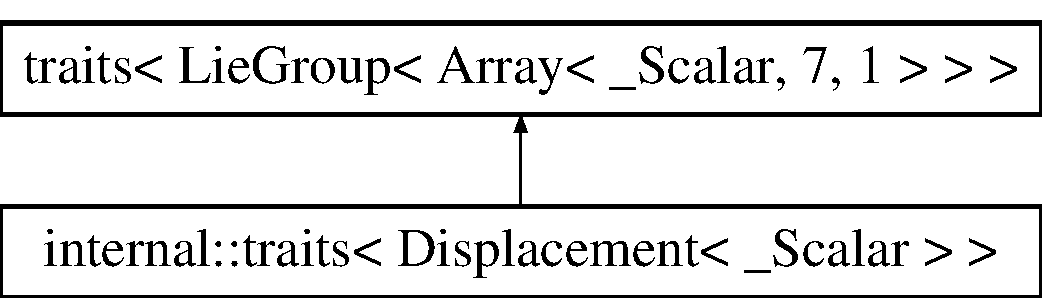
\includegraphics[height=2.000000cm]{structinternal_1_1traits_3_01_displacement_3_01___scalar_01_4_01_4}
\end{center}
\end{figure}
\subsection*{Public Types}
\begin{DoxyCompactItemize}
\item 
typedef \hyperlink{class_displacement}{Displacement}$<$ \+\_\+\+Scalar $>$ \hyperlink{structinternal_1_1traits_3_01_displacement_3_01___scalar_01_4_01_4_af6e4238e8d42d544cfad72771d52f368}{Plain\+Object}
\item 
typedef \+\_\+\+Scalar \hyperlink{structinternal_1_1traits_3_01_displacement_3_01___scalar_01_4_01_4_a599bdd94fc645c9d06a36202d58f0ed8}{Scalar}
\end{DoxyCompactItemize}


\subsection{Detailed Description}
\subsubsection*{template$<$typename \+\_\+\+Scalar$>$\newline
struct internal\+::traits$<$ Displacement$<$ \+\_\+\+Scalar $>$ $>$}



Definition at line 141 of file Displacement.\+h.



\subsection{Member Typedef Documentation}
\hypertarget{structinternal_1_1traits_3_01_displacement_3_01___scalar_01_4_01_4_af6e4238e8d42d544cfad72771d52f368}{}\label{structinternal_1_1traits_3_01_displacement_3_01___scalar_01_4_01_4_af6e4238e8d42d544cfad72771d52f368} 
\index{internal\+::traits$<$ Displacement$<$ \+\_\+\+Scalar $>$ $>$@{internal\+::traits$<$ Displacement$<$ \+\_\+\+Scalar $>$ $>$}!Plain\+Object@{Plain\+Object}}
\index{Plain\+Object@{Plain\+Object}!internal\+::traits$<$ Displacement$<$ \+\_\+\+Scalar $>$ $>$@{internal\+::traits$<$ Displacement$<$ \+\_\+\+Scalar $>$ $>$}}
\subsubsection{\texorpdfstring{Plain\+Object}{PlainObject}}
{\footnotesize\ttfamily template$<$typename \+\_\+\+Scalar $>$ \\
typedef \hyperlink{class_displacement}{Displacement}$<$\+\_\+\+Scalar$>$ internal\+::traits$<$ \hyperlink{class_displacement}{Displacement}$<$ \+\_\+\+Scalar $>$ $>$\+::\hyperlink{structinternal_1_1traits_3_01_displacement_3_01___scalar_01_4_01_4_af6e4238e8d42d544cfad72771d52f368}{Plain\+Object}}



Definition at line 143 of file Displacement.\+h.

\hypertarget{structinternal_1_1traits_3_01_displacement_3_01___scalar_01_4_01_4_a599bdd94fc645c9d06a36202d58f0ed8}{}\label{structinternal_1_1traits_3_01_displacement_3_01___scalar_01_4_01_4_a599bdd94fc645c9d06a36202d58f0ed8} 
\index{internal\+::traits$<$ Displacement$<$ \+\_\+\+Scalar $>$ $>$@{internal\+::traits$<$ Displacement$<$ \+\_\+\+Scalar $>$ $>$}!Scalar@{Scalar}}
\index{Scalar@{Scalar}!internal\+::traits$<$ Displacement$<$ \+\_\+\+Scalar $>$ $>$@{internal\+::traits$<$ Displacement$<$ \+\_\+\+Scalar $>$ $>$}}
\subsubsection{\texorpdfstring{Scalar}{Scalar}}
{\footnotesize\ttfamily template$<$typename \+\_\+\+Scalar $>$ \\
typedef \+\_\+\+Scalar internal\+::traits$<$ \hyperlink{class_displacement}{Displacement}$<$ \+\_\+\+Scalar $>$ $>$\+::\hyperlink{structinternal_1_1traits_3_01_displacement_3_01___scalar_01_4_01_4_a599bdd94fc645c9d06a36202d58f0ed8}{Scalar}}



Definition at line 144 of file Displacement.\+h.



The documentation for this struct was generated from the following file\+:\begin{DoxyCompactItemize}
\item 
/\+Users/\+Ryan/\+Code/codyco-\/superbuild/libraries/\+Eigen\+Lgsm/unsupported/\+Eigen/src/\+Lgsm/\hyperlink{_displacement_8h}{Displacement.\+h}\end{DoxyCompactItemize}

\hypertarget{structinternal_1_1traits_3_01_lie_algebra_3_01_a_01_4_01_4}{}\section{internal\+:\+:traits$<$ Lie\+Algebra$<$ A $>$ $>$ Struct Template Reference}
\label{structinternal_1_1traits_3_01_lie_algebra_3_01_a_01_4_01_4}\index{internal\+::traits$<$ Lie\+Algebra$<$ A $>$ $>$@{internal\+::traits$<$ Lie\+Algebra$<$ A $>$ $>$}}


{\ttfamily \#include $<$Lie\+Algebra.\+h$>$}

Inheritance diagram for internal\+:\+:traits$<$ Lie\+Algebra$<$ A $>$ $>$\+:\begin{figure}[H]
\begin{center}
\leavevmode
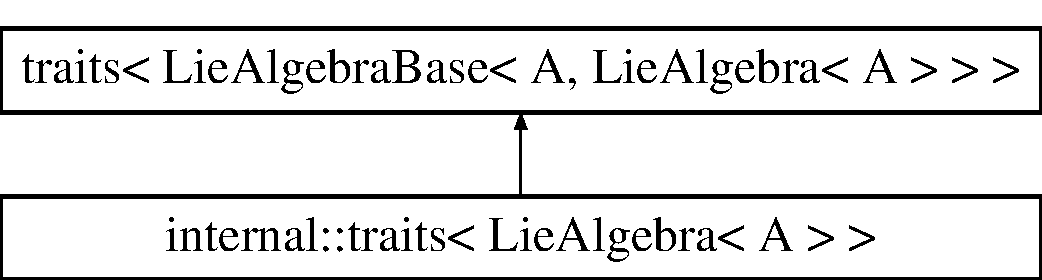
\includegraphics[height=2.000000cm]{structinternal_1_1traits_3_01_lie_algebra_3_01_a_01_4_01_4}
\end{center}
\end{figure}
\subsection*{Public Types}
\begin{DoxyCompactItemize}
\item 
typedef A \hyperlink{structinternal_1_1traits_3_01_lie_algebra_3_01_a_01_4_01_4_a001bd1e57bb80cc75d486c92b152d2f2}{Coefficients}
\end{DoxyCompactItemize}


\subsection{Detailed Description}
\subsubsection*{template$<$class A$>$\newline
struct internal\+::traits$<$ Lie\+Algebra$<$ A $>$ $>$}



Definition at line 152 of file Lie\+Algebra.\+h.



\subsection{Member Typedef Documentation}
\hypertarget{structinternal_1_1traits_3_01_lie_algebra_3_01_a_01_4_01_4_a001bd1e57bb80cc75d486c92b152d2f2}{}\label{structinternal_1_1traits_3_01_lie_algebra_3_01_a_01_4_01_4_a001bd1e57bb80cc75d486c92b152d2f2} 
\index{internal\+::traits$<$ Lie\+Algebra$<$ A $>$ $>$@{internal\+::traits$<$ Lie\+Algebra$<$ A $>$ $>$}!Coefficients@{Coefficients}}
\index{Coefficients@{Coefficients}!internal\+::traits$<$ Lie\+Algebra$<$ A $>$ $>$@{internal\+::traits$<$ Lie\+Algebra$<$ A $>$ $>$}}
\subsubsection{\texorpdfstring{Coefficients}{Coefficients}}
{\footnotesize\ttfamily template$<$class A $>$ \\
typedef A internal\+::traits$<$ \hyperlink{class_lie_algebra}{Lie\+Algebra}$<$ A $>$ $>$\+::\hyperlink{structinternal_1_1traits_3_01_lie_algebra_3_01_a_01_4_01_4_a001bd1e57bb80cc75d486c92b152d2f2}{Coefficients}}



Definition at line 154 of file Lie\+Algebra.\+h.



The documentation for this struct was generated from the following file\+:\begin{DoxyCompactItemize}
\item 
/\+Users/\+Ryan/\+Code/codyco-\/superbuild/libraries/\+Eigen\+Lgsm/unsupported/\+Eigen/src/\+Lgsm/\hyperlink{_lie_algebra_8h}{Lie\+Algebra.\+h}\end{DoxyCompactItemize}

\hypertarget{structinternal_1_1traits_3_01_lie_algebra_3_01_matrix_3_01_scalar_00_013_00_011_01_4_01_4_01_4}{}\section{internal\+:\+:traits$<$ Lie\+Algebra$<$ Matrix$<$ Scalar, 3, 1 $>$ $>$ $>$ Struct Template Reference}
\label{structinternal_1_1traits_3_01_lie_algebra_3_01_matrix_3_01_scalar_00_013_00_011_01_4_01_4_01_4}\index{internal\+::traits$<$ Lie\+Algebra$<$ Matrix$<$ Scalar, 3, 1 $>$ $>$ $>$@{internal\+::traits$<$ Lie\+Algebra$<$ Matrix$<$ Scalar, 3, 1 $>$ $>$ $>$}}


{\ttfamily \#include $<$Lie\+Algebra\+\_\+so3.\+h$>$}

Inheritance diagram for internal\+:\+:traits$<$ Lie\+Algebra$<$ Matrix$<$ Scalar, 3, 1 $>$ $>$ $>$\+:\begin{figure}[H]
\begin{center}
\leavevmode
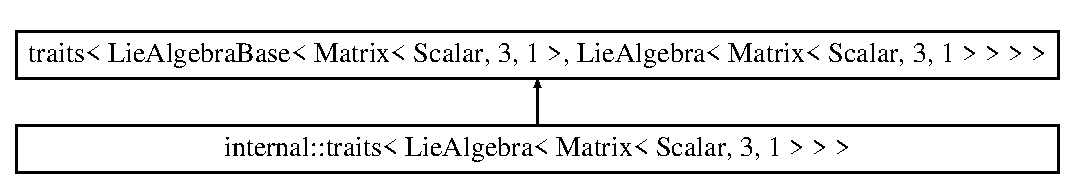
\includegraphics[height=2.000000cm]{structinternal_1_1traits_3_01_lie_algebra_3_01_matrix_3_01_scalar_00_013_00_011_01_4_01_4_01_4}
\end{center}
\end{figure}
\subsection*{Public Types}
\begin{DoxyCompactItemize}
\item 
typedef Matrix$<$ Scalar, 3, 1 $>$ \hyperlink{structinternal_1_1traits_3_01_lie_algebra_3_01_matrix_3_01_scalar_00_013_00_011_01_4_01_4_01_4_a8ef1db6f76e3e2ca5f0aff3609d06f7c}{Coefficients}
\item 
typedef \hyperlink{class_lie_group}{Lie\+Group}$<$ Quaternion$<$ Scalar $>$ $>$ \hyperlink{structinternal_1_1traits_3_01_lie_algebra_3_01_matrix_3_01_scalar_00_013_00_011_01_4_01_4_01_4_a55e3fb1ea655ef4f7582a54857fe98b1}{Group}
\end{DoxyCompactItemize}


\subsection{Detailed Description}
\subsubsection*{template$<$typename Scalar$>$\newline
struct internal\+::traits$<$ Lie\+Algebra$<$ Matrix$<$ Scalar, 3, 1 $>$ $>$ $>$}



Definition at line 298 of file Lie\+Algebra\+\_\+so3.\+h.



\subsection{Member Typedef Documentation}
\hypertarget{structinternal_1_1traits_3_01_lie_algebra_3_01_matrix_3_01_scalar_00_013_00_011_01_4_01_4_01_4_a8ef1db6f76e3e2ca5f0aff3609d06f7c}{}\label{structinternal_1_1traits_3_01_lie_algebra_3_01_matrix_3_01_scalar_00_013_00_011_01_4_01_4_01_4_a8ef1db6f76e3e2ca5f0aff3609d06f7c} 
\index{internal\+::traits$<$ Lie\+Algebra$<$ Matrix$<$ Scalar, 3, 1 $>$ $>$ $>$@{internal\+::traits$<$ Lie\+Algebra$<$ Matrix$<$ Scalar, 3, 1 $>$ $>$ $>$}!Coefficients@{Coefficients}}
\index{Coefficients@{Coefficients}!internal\+::traits$<$ Lie\+Algebra$<$ Matrix$<$ Scalar, 3, 1 $>$ $>$ $>$@{internal\+::traits$<$ Lie\+Algebra$<$ Matrix$<$ Scalar, 3, 1 $>$ $>$ $>$}}
\subsubsection{\texorpdfstring{Coefficients}{Coefficients}}
{\footnotesize\ttfamily template$<$typename Scalar $>$ \\
typedef Matrix$<$Scalar, 3, 1$>$ internal\+::traits$<$ \hyperlink{class_lie_algebra}{Lie\+Algebra}$<$ Matrix$<$ Scalar, 3, 1 $>$ $>$ $>$\+::\hyperlink{structinternal_1_1traits_3_01_lie_algebra_3_01_matrix_3_01_scalar_00_013_00_011_01_4_01_4_01_4_a8ef1db6f76e3e2ca5f0aff3609d06f7c}{Coefficients}}



Definition at line 301 of file Lie\+Algebra\+\_\+so3.\+h.

\hypertarget{structinternal_1_1traits_3_01_lie_algebra_3_01_matrix_3_01_scalar_00_013_00_011_01_4_01_4_01_4_a55e3fb1ea655ef4f7582a54857fe98b1}{}\label{structinternal_1_1traits_3_01_lie_algebra_3_01_matrix_3_01_scalar_00_013_00_011_01_4_01_4_01_4_a55e3fb1ea655ef4f7582a54857fe98b1} 
\index{internal\+::traits$<$ Lie\+Algebra$<$ Matrix$<$ Scalar, 3, 1 $>$ $>$ $>$@{internal\+::traits$<$ Lie\+Algebra$<$ Matrix$<$ Scalar, 3, 1 $>$ $>$ $>$}!Group@{Group}}
\index{Group@{Group}!internal\+::traits$<$ Lie\+Algebra$<$ Matrix$<$ Scalar, 3, 1 $>$ $>$ $>$@{internal\+::traits$<$ Lie\+Algebra$<$ Matrix$<$ Scalar, 3, 1 $>$ $>$ $>$}}
\subsubsection{\texorpdfstring{Group}{Group}}
{\footnotesize\ttfamily template$<$typename Scalar $>$ \\
typedef \hyperlink{class_lie_group}{Lie\+Group}$<$Quaternion$<$Scalar$>$ $>$ internal\+::traits$<$ \hyperlink{class_lie_algebra}{Lie\+Algebra}$<$ Matrix$<$ Scalar, 3, 1 $>$ $>$ $>$\+::\hyperlink{structinternal_1_1traits_3_01_lie_algebra_3_01_matrix_3_01_scalar_00_013_00_011_01_4_01_4_01_4_a55e3fb1ea655ef4f7582a54857fe98b1}{Group}}



Definition at line 302 of file Lie\+Algebra\+\_\+so3.\+h.



The documentation for this struct was generated from the following file\+:\begin{DoxyCompactItemize}
\item 
/\+Users/\+Ryan/\+Code/codyco-\/superbuild/libraries/\+Eigen\+Lgsm/unsupported/\+Eigen/src/\+Lgsm/\hyperlink{_lie_algebra__so3_8h}{Lie\+Algebra\+\_\+so3.\+h}\end{DoxyCompactItemize}

\hypertarget{structinternal_1_1traits_3_01_lie_algebra_3_01_matrix_3_01_scalar_00_016_00_011_01_4_01_4_01_4}{}\section{internal\+:\+:traits$<$ Lie\+Algebra$<$ Matrix$<$ Scalar, 6, 1 $>$ $>$ $>$ Struct Template Reference}
\label{structinternal_1_1traits_3_01_lie_algebra_3_01_matrix_3_01_scalar_00_016_00_011_01_4_01_4_01_4}\index{internal\+::traits$<$ Lie\+Algebra$<$ Matrix$<$ Scalar, 6, 1 $>$ $>$ $>$@{internal\+::traits$<$ Lie\+Algebra$<$ Matrix$<$ Scalar, 6, 1 $>$ $>$ $>$}}


{\ttfamily \#include $<$Lie\+Algebra\+\_\+se3.\+h$>$}

Inheritance diagram for internal\+:\+:traits$<$ Lie\+Algebra$<$ Matrix$<$ Scalar, 6, 1 $>$ $>$ $>$\+:\begin{figure}[H]
\begin{center}
\leavevmode
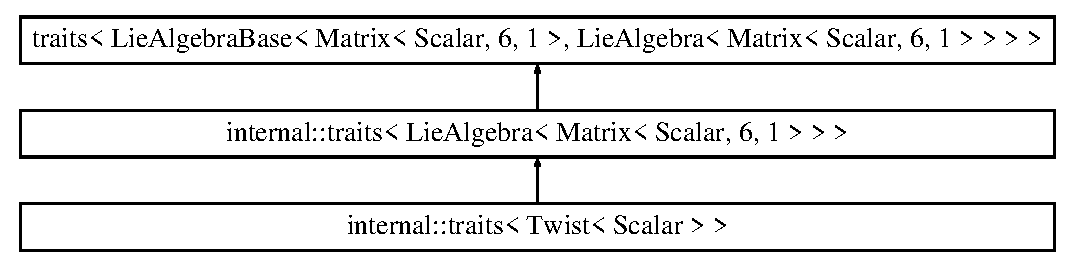
\includegraphics[height=3.000000cm]{structinternal_1_1traits_3_01_lie_algebra_3_01_matrix_3_01_scalar_00_016_00_011_01_4_01_4_01_4}
\end{center}
\end{figure}
\subsection*{Public Types}
\begin{DoxyCompactItemize}
\item 
typedef Matrix$<$ Scalar, 6, 1 $>$ \hyperlink{structinternal_1_1traits_3_01_lie_algebra_3_01_matrix_3_01_scalar_00_016_00_011_01_4_01_4_01_4_a24207cc49d00e538b9dac7329edc23e6}{Coefficients}
\item 
typedef \hyperlink{class_lie_group}{Lie\+Group}$<$ Array$<$ Scalar, 7, 1 $>$ $>$ \hyperlink{structinternal_1_1traits_3_01_lie_algebra_3_01_matrix_3_01_scalar_00_016_00_011_01_4_01_4_01_4_a2a6e55a56a1c0c3b97c50cb8598ac55a}{Group}
\end{DoxyCompactItemize}


\subsection{Detailed Description}
\subsubsection*{template$<$typename Scalar$>$\newline
struct internal\+::traits$<$ Lie\+Algebra$<$ Matrix$<$ Scalar, 6, 1 $>$ $>$ $>$}



Definition at line 240 of file Lie\+Algebra\+\_\+se3.\+h.



\subsection{Member Typedef Documentation}
\hypertarget{structinternal_1_1traits_3_01_lie_algebra_3_01_matrix_3_01_scalar_00_016_00_011_01_4_01_4_01_4_a24207cc49d00e538b9dac7329edc23e6}{}\label{structinternal_1_1traits_3_01_lie_algebra_3_01_matrix_3_01_scalar_00_016_00_011_01_4_01_4_01_4_a24207cc49d00e538b9dac7329edc23e6} 
\index{internal\+::traits$<$ Lie\+Algebra$<$ Matrix$<$ Scalar, 6, 1 $>$ $>$ $>$@{internal\+::traits$<$ Lie\+Algebra$<$ Matrix$<$ Scalar, 6, 1 $>$ $>$ $>$}!Coefficients@{Coefficients}}
\index{Coefficients@{Coefficients}!internal\+::traits$<$ Lie\+Algebra$<$ Matrix$<$ Scalar, 6, 1 $>$ $>$ $>$@{internal\+::traits$<$ Lie\+Algebra$<$ Matrix$<$ Scalar, 6, 1 $>$ $>$ $>$}}
\subsubsection{\texorpdfstring{Coefficients}{Coefficients}}
{\footnotesize\ttfamily template$<$typename Scalar $>$ \\
typedef Matrix$<$Scalar, 6, 1$>$ internal\+::traits$<$ \hyperlink{class_lie_algebra}{Lie\+Algebra}$<$ Matrix$<$ Scalar, 6, 1 $>$ $>$ $>$\+::\hyperlink{structinternal_1_1traits_3_01_lie_algebra_3_01_matrix_3_01_scalar_00_016_00_011_01_4_01_4_01_4_a24207cc49d00e538b9dac7329edc23e6}{Coefficients}}



Definition at line 243 of file Lie\+Algebra\+\_\+se3.\+h.

\hypertarget{structinternal_1_1traits_3_01_lie_algebra_3_01_matrix_3_01_scalar_00_016_00_011_01_4_01_4_01_4_a2a6e55a56a1c0c3b97c50cb8598ac55a}{}\label{structinternal_1_1traits_3_01_lie_algebra_3_01_matrix_3_01_scalar_00_016_00_011_01_4_01_4_01_4_a2a6e55a56a1c0c3b97c50cb8598ac55a} 
\index{internal\+::traits$<$ Lie\+Algebra$<$ Matrix$<$ Scalar, 6, 1 $>$ $>$ $>$@{internal\+::traits$<$ Lie\+Algebra$<$ Matrix$<$ Scalar, 6, 1 $>$ $>$ $>$}!Group@{Group}}
\index{Group@{Group}!internal\+::traits$<$ Lie\+Algebra$<$ Matrix$<$ Scalar, 6, 1 $>$ $>$ $>$@{internal\+::traits$<$ Lie\+Algebra$<$ Matrix$<$ Scalar, 6, 1 $>$ $>$ $>$}}
\subsubsection{\texorpdfstring{Group}{Group}}
{\footnotesize\ttfamily template$<$typename Scalar $>$ \\
typedef \hyperlink{class_lie_group}{Lie\+Group}$<$Array$<$Scalar, 7, 1$>$ $>$ internal\+::traits$<$ \hyperlink{class_lie_algebra}{Lie\+Algebra}$<$ Matrix$<$ Scalar, 6, 1 $>$ $>$ $>$\+::\hyperlink{structinternal_1_1traits_3_01_lie_algebra_3_01_matrix_3_01_scalar_00_016_00_011_01_4_01_4_01_4_a2a6e55a56a1c0c3b97c50cb8598ac55a}{Group}}



Definition at line 244 of file Lie\+Algebra\+\_\+se3.\+h.



The documentation for this struct was generated from the following file\+:\begin{DoxyCompactItemize}
\item 
/\+Users/\+Ryan/\+Code/codyco-\/superbuild/libraries/\+Eigen\+Lgsm/unsupported/\+Eigen/src/\+Lgsm/\hyperlink{_lie_algebra__se3_8h}{Lie\+Algebra\+\_\+se3.\+h}\end{DoxyCompactItemize}

\hypertarget{structinternal_1_1traits_3_01_lie_algebra_base_3_01_a_00_01_derived_01_4_01_4}{}\section{internal\+:\+:traits$<$ Lie\+Algebra\+Base$<$ A, Derived $>$ $>$ Struct Template Reference}
\label{structinternal_1_1traits_3_01_lie_algebra_base_3_01_a_00_01_derived_01_4_01_4}\index{internal\+::traits$<$ Lie\+Algebra\+Base$<$ A, Derived $>$ $>$@{internal\+::traits$<$ Lie\+Algebra\+Base$<$ A, Derived $>$ $>$}}


{\ttfamily \#include $<$Lie\+Algebra.\+h$>$}

Inheritance diagram for internal\+:\+:traits$<$ Lie\+Algebra\+Base$<$ A, Derived $>$ $>$\+:\begin{figure}[H]
\begin{center}
\leavevmode
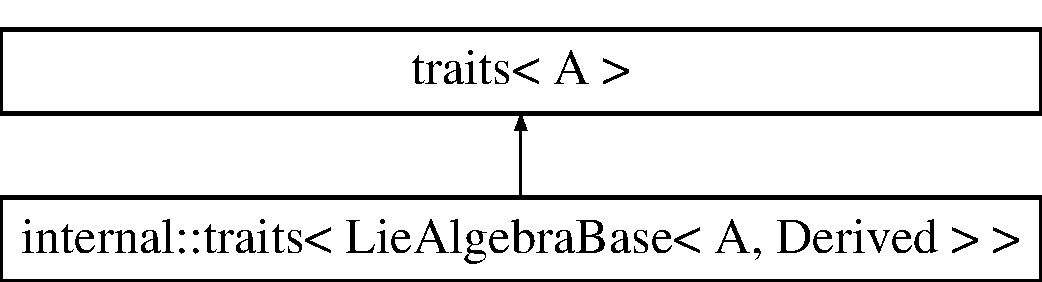
\includegraphics[height=2.000000cm]{structinternal_1_1traits_3_01_lie_algebra_base_3_01_a_00_01_derived_01_4_01_4}
\end{center}
\end{figure}


\subsection{Detailed Description}
\subsubsection*{template$<$class A, class Derived$>$\newline
struct internal\+::traits$<$ Lie\+Algebra\+Base$<$ A, Derived $>$ $>$}



Definition at line 31 of file Lie\+Algebra.\+h.



The documentation for this struct was generated from the following file\+:\begin{DoxyCompactItemize}
\item 
/\+Users/\+Ryan/\+Code/codyco-\/superbuild/libraries/\+Eigen\+Lgsm/unsupported/\+Eigen/src/\+Lgsm/\hyperlink{_lie_algebra_8h}{Lie\+Algebra.\+h}\end{DoxyCompactItemize}

\hypertarget{structinternal_1_1traits_3_01_lie_algebra_dual_3_01_a_01_4_01_4}{}\section{internal\+:\+:traits$<$ Lie\+Algebra\+Dual$<$ A $>$ $>$ Struct Template Reference}
\label{structinternal_1_1traits_3_01_lie_algebra_dual_3_01_a_01_4_01_4}\index{internal\+::traits$<$ Lie\+Algebra\+Dual$<$ A $>$ $>$@{internal\+::traits$<$ Lie\+Algebra\+Dual$<$ A $>$ $>$}}


{\ttfamily \#include $<$Lie\+Algebra.\+h$>$}

Inheritance diagram for internal\+:\+:traits$<$ Lie\+Algebra\+Dual$<$ A $>$ $>$\+:\begin{figure}[H]
\begin{center}
\leavevmode
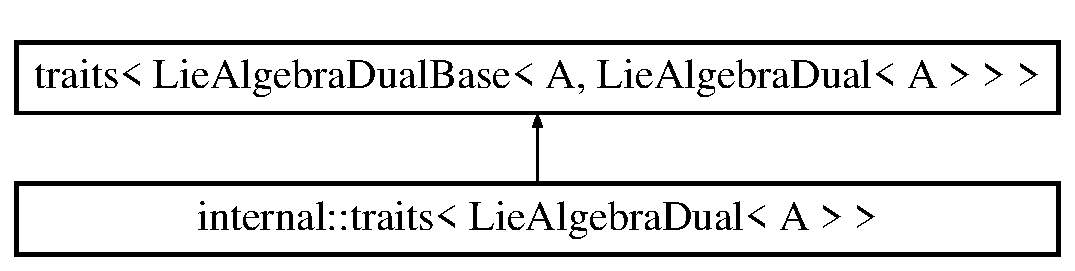
\includegraphics[height=2.000000cm]{structinternal_1_1traits_3_01_lie_algebra_dual_3_01_a_01_4_01_4}
\end{center}
\end{figure}
\subsection*{Public Types}
\begin{DoxyCompactItemize}
\item 
typedef A \hyperlink{structinternal_1_1traits_3_01_lie_algebra_dual_3_01_a_01_4_01_4_a1272ac68a65e84810584f5a54eabe4bc}{Coefficients}
\end{DoxyCompactItemize}


\subsection{Detailed Description}
\subsubsection*{template$<$class A$>$\newline
struct internal\+::traits$<$ Lie\+Algebra\+Dual$<$ A $>$ $>$}



Definition at line 200 of file Lie\+Algebra.\+h.



\subsection{Member Typedef Documentation}
\hypertarget{structinternal_1_1traits_3_01_lie_algebra_dual_3_01_a_01_4_01_4_a1272ac68a65e84810584f5a54eabe4bc}{}\label{structinternal_1_1traits_3_01_lie_algebra_dual_3_01_a_01_4_01_4_a1272ac68a65e84810584f5a54eabe4bc} 
\index{internal\+::traits$<$ Lie\+Algebra\+Dual$<$ A $>$ $>$@{internal\+::traits$<$ Lie\+Algebra\+Dual$<$ A $>$ $>$}!Coefficients@{Coefficients}}
\index{Coefficients@{Coefficients}!internal\+::traits$<$ Lie\+Algebra\+Dual$<$ A $>$ $>$@{internal\+::traits$<$ Lie\+Algebra\+Dual$<$ A $>$ $>$}}
\subsubsection{\texorpdfstring{Coefficients}{Coefficients}}
{\footnotesize\ttfamily template$<$class A $>$ \\
typedef A internal\+::traits$<$ \hyperlink{class_lie_algebra_dual}{Lie\+Algebra\+Dual}$<$ A $>$ $>$\+::\hyperlink{structinternal_1_1traits_3_01_lie_algebra_dual_3_01_a_01_4_01_4_a1272ac68a65e84810584f5a54eabe4bc}{Coefficients}}



Definition at line 202 of file Lie\+Algebra.\+h.



The documentation for this struct was generated from the following file\+:\begin{DoxyCompactItemize}
\item 
/\+Users/\+Ryan/\+Code/codyco-\/superbuild/libraries/\+Eigen\+Lgsm/unsupported/\+Eigen/src/\+Lgsm/\hyperlink{_lie_algebra_8h}{Lie\+Algebra.\+h}\end{DoxyCompactItemize}

\hypertarget{structinternal_1_1traits_3_01_lie_algebra_dual_3_01_matrix_3_01_scalar_00_013_00_011_01_4_01_4_01_4}{}\section{internal\+:\+:traits$<$ Lie\+Algebra\+Dual$<$ Matrix$<$ Scalar, 3, 1 $>$ $>$ $>$ Struct Template Reference}
\label{structinternal_1_1traits_3_01_lie_algebra_dual_3_01_matrix_3_01_scalar_00_013_00_011_01_4_01_4_01_4}\index{internal\+::traits$<$ Lie\+Algebra\+Dual$<$ Matrix$<$ Scalar, 3, 1 $>$ $>$ $>$@{internal\+::traits$<$ Lie\+Algebra\+Dual$<$ Matrix$<$ Scalar, 3, 1 $>$ $>$ $>$}}


{\ttfamily \#include $<$Lie\+Algebra\+\_\+so3.\+h$>$}

Inheritance diagram for internal\+:\+:traits$<$ Lie\+Algebra\+Dual$<$ Matrix$<$ Scalar, 3, 1 $>$ $>$ $>$\+:\begin{figure}[H]
\begin{center}
\leavevmode
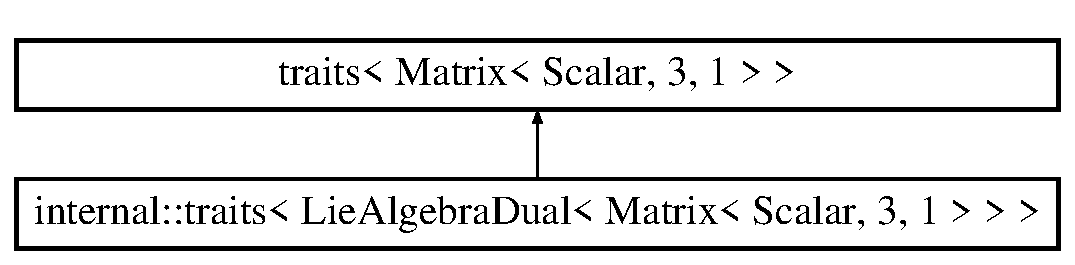
\includegraphics[height=2.000000cm]{structinternal_1_1traits_3_01_lie_algebra_dual_3_01_matrix_3_01_scalar_00_013_00_011_01_4_01_4_01_4}
\end{center}
\end{figure}
\subsection*{Public Types}
\begin{DoxyCompactItemize}
\item 
typedef Matrix$<$ Scalar, 3, 1 $>$ \hyperlink{structinternal_1_1traits_3_01_lie_algebra_dual_3_01_matrix_3_01_scalar_00_013_00_011_01_4_01_4_01_4_a80495946885356581543f8de93844103}{Coefficients}
\item 
typedef \hyperlink{class_lie_group}{Lie\+Group}$<$ Quaternion$<$ Scalar $>$ $>$ \hyperlink{structinternal_1_1traits_3_01_lie_algebra_dual_3_01_matrix_3_01_scalar_00_013_00_011_01_4_01_4_01_4_a05cfaae13397aaf0d8ece656959c0bfb}{Group}
\end{DoxyCompactItemize}


\subsection{Detailed Description}
\subsubsection*{template$<$typename Scalar$>$\newline
struct internal\+::traits$<$ Lie\+Algebra\+Dual$<$ Matrix$<$ Scalar, 3, 1 $>$ $>$ $>$}



Definition at line 258 of file Lie\+Algebra\+\_\+so3.\+h.



\subsection{Member Typedef Documentation}
\hypertarget{structinternal_1_1traits_3_01_lie_algebra_dual_3_01_matrix_3_01_scalar_00_013_00_011_01_4_01_4_01_4_a80495946885356581543f8de93844103}{}\label{structinternal_1_1traits_3_01_lie_algebra_dual_3_01_matrix_3_01_scalar_00_013_00_011_01_4_01_4_01_4_a80495946885356581543f8de93844103} 
\index{internal\+::traits$<$ Lie\+Algebra\+Dual$<$ Matrix$<$ Scalar, 3, 1 $>$ $>$ $>$@{internal\+::traits$<$ Lie\+Algebra\+Dual$<$ Matrix$<$ Scalar, 3, 1 $>$ $>$ $>$}!Coefficients@{Coefficients}}
\index{Coefficients@{Coefficients}!internal\+::traits$<$ Lie\+Algebra\+Dual$<$ Matrix$<$ Scalar, 3, 1 $>$ $>$ $>$@{internal\+::traits$<$ Lie\+Algebra\+Dual$<$ Matrix$<$ Scalar, 3, 1 $>$ $>$ $>$}}
\subsubsection{\texorpdfstring{Coefficients}{Coefficients}}
{\footnotesize\ttfamily template$<$typename Scalar $>$ \\
typedef Matrix$<$Scalar, 3, 1$>$ internal\+::traits$<$ \hyperlink{class_lie_algebra_dual}{Lie\+Algebra\+Dual}$<$ Matrix$<$ Scalar, 3, 1 $>$ $>$ $>$\+::\hyperlink{structinternal_1_1traits_3_01_lie_algebra_dual_3_01_matrix_3_01_scalar_00_013_00_011_01_4_01_4_01_4_a80495946885356581543f8de93844103}{Coefficients}}



Definition at line 260 of file Lie\+Algebra\+\_\+so3.\+h.

\hypertarget{structinternal_1_1traits_3_01_lie_algebra_dual_3_01_matrix_3_01_scalar_00_013_00_011_01_4_01_4_01_4_a05cfaae13397aaf0d8ece656959c0bfb}{}\label{structinternal_1_1traits_3_01_lie_algebra_dual_3_01_matrix_3_01_scalar_00_013_00_011_01_4_01_4_01_4_a05cfaae13397aaf0d8ece656959c0bfb} 
\index{internal\+::traits$<$ Lie\+Algebra\+Dual$<$ Matrix$<$ Scalar, 3, 1 $>$ $>$ $>$@{internal\+::traits$<$ Lie\+Algebra\+Dual$<$ Matrix$<$ Scalar, 3, 1 $>$ $>$ $>$}!Group@{Group}}
\index{Group@{Group}!internal\+::traits$<$ Lie\+Algebra\+Dual$<$ Matrix$<$ Scalar, 3, 1 $>$ $>$ $>$@{internal\+::traits$<$ Lie\+Algebra\+Dual$<$ Matrix$<$ Scalar, 3, 1 $>$ $>$ $>$}}
\subsubsection{\texorpdfstring{Group}{Group}}
{\footnotesize\ttfamily template$<$typename Scalar $>$ \\
typedef \hyperlink{class_lie_group}{Lie\+Group}$<$Quaternion$<$Scalar$>$ $>$ internal\+::traits$<$ \hyperlink{class_lie_algebra_dual}{Lie\+Algebra\+Dual}$<$ Matrix$<$ Scalar, 3, 1 $>$ $>$ $>$\+::\hyperlink{structinternal_1_1traits_3_01_lie_algebra_dual_3_01_matrix_3_01_scalar_00_013_00_011_01_4_01_4_01_4_a05cfaae13397aaf0d8ece656959c0bfb}{Group}}



Definition at line 261 of file Lie\+Algebra\+\_\+so3.\+h.



The documentation for this struct was generated from the following file\+:\begin{DoxyCompactItemize}
\item 
/\+Users/\+Ryan/\+Code/codyco-\/superbuild/libraries/\+Eigen\+Lgsm/unsupported/\+Eigen/src/\+Lgsm/\hyperlink{_lie_algebra__so3_8h}{Lie\+Algebra\+\_\+so3.\+h}\end{DoxyCompactItemize}

\hypertarget{structinternal_1_1traits_3_01_lie_algebra_dual_base_3_01_a_00_01_derived_01_4_01_4}{}\section{internal\+:\+:traits$<$ Lie\+Algebra\+Dual\+Base$<$ A, Derived $>$ $>$ Struct Template Reference}
\label{structinternal_1_1traits_3_01_lie_algebra_dual_base_3_01_a_00_01_derived_01_4_01_4}\index{internal\+::traits$<$ Lie\+Algebra\+Dual\+Base$<$ A, Derived $>$ $>$@{internal\+::traits$<$ Lie\+Algebra\+Dual\+Base$<$ A, Derived $>$ $>$}}


{\ttfamily \#include $<$Lie\+Algebra.\+h$>$}

Inheritance diagram for internal\+:\+:traits$<$ Lie\+Algebra\+Dual\+Base$<$ A, Derived $>$ $>$\+:\begin{figure}[H]
\begin{center}
\leavevmode
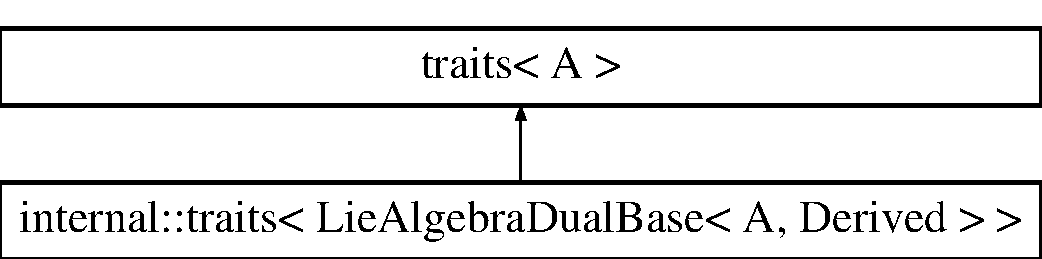
\includegraphics[height=2.000000cm]{structinternal_1_1traits_3_01_lie_algebra_dual_base_3_01_a_00_01_derived_01_4_01_4}
\end{center}
\end{figure}


\subsection{Detailed Description}
\subsubsection*{template$<$class A, class Derived$>$\newline
struct internal\+::traits$<$ Lie\+Algebra\+Dual\+Base$<$ A, Derived $>$ $>$}



Definition at line 96 of file Lie\+Algebra.\+h.



The documentation for this struct was generated from the following file\+:\begin{DoxyCompactItemize}
\item 
/\+Users/\+Ryan/\+Code/codyco-\/superbuild/libraries/\+Eigen\+Lgsm/unsupported/\+Eigen/src/\+Lgsm/\hyperlink{_lie_algebra_8h}{Lie\+Algebra.\+h}\end{DoxyCompactItemize}

\hypertarget{structinternal_1_1traits_3_01_lie_group_3_01_g_01_4_01_4}{}\section{internal\+:\+:traits$<$ Lie\+Group$<$ G $>$ $>$ Struct Template Reference}
\label{structinternal_1_1traits_3_01_lie_group_3_01_g_01_4_01_4}\index{internal\+::traits$<$ Lie\+Group$<$ G $>$ $>$@{internal\+::traits$<$ Lie\+Group$<$ G $>$ $>$}}


{\ttfamily \#include $<$Lie\+Group.\+h$>$}

Inheritance diagram for internal\+:\+:traits$<$ Lie\+Group$<$ G $>$ $>$\+:\begin{figure}[H]
\begin{center}
\leavevmode
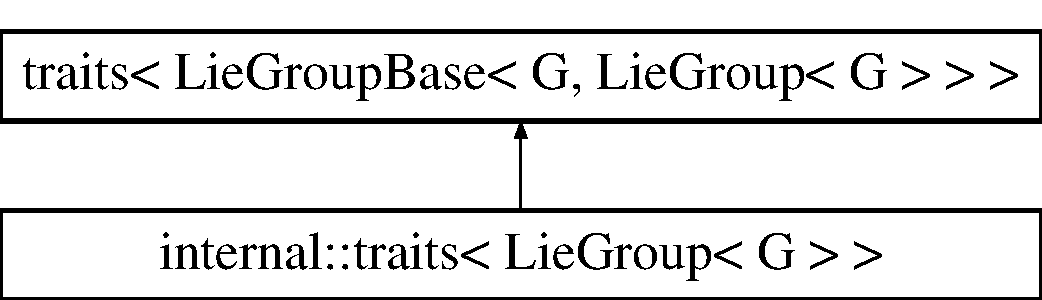
\includegraphics[height=2.000000cm]{structinternal_1_1traits_3_01_lie_group_3_01_g_01_4_01_4}
\end{center}
\end{figure}
\subsection*{Public Types}
\begin{DoxyCompactItemize}
\item 
typedef G \hyperlink{structinternal_1_1traits_3_01_lie_group_3_01_g_01_4_01_4_adfb0de0a4ac03ebf58b0e6d9372e831d}{Coefficients}
\item 
typedef G\+::\+Scalar \hyperlink{structinternal_1_1traits_3_01_lie_group_3_01_g_01_4_01_4_ab4c105288bd0027999a766a8ca7ac9c5}{Scalar}
\end{DoxyCompactItemize}


\subsection{Detailed Description}
\subsubsection*{template$<$class G$>$\newline
struct internal\+::traits$<$ Lie\+Group$<$ G $>$ $>$}



Definition at line 96 of file Lie\+Group.\+h.



\subsection{Member Typedef Documentation}
\hypertarget{structinternal_1_1traits_3_01_lie_group_3_01_g_01_4_01_4_adfb0de0a4ac03ebf58b0e6d9372e831d}{}\label{structinternal_1_1traits_3_01_lie_group_3_01_g_01_4_01_4_adfb0de0a4ac03ebf58b0e6d9372e831d} 
\index{internal\+::traits$<$ Lie\+Group$<$ G $>$ $>$@{internal\+::traits$<$ Lie\+Group$<$ G $>$ $>$}!Coefficients@{Coefficients}}
\index{Coefficients@{Coefficients}!internal\+::traits$<$ Lie\+Group$<$ G $>$ $>$@{internal\+::traits$<$ Lie\+Group$<$ G $>$ $>$}}
\subsubsection{\texorpdfstring{Coefficients}{Coefficients}}
{\footnotesize\ttfamily template$<$class G $>$ \\
typedef G internal\+::traits$<$ \hyperlink{class_lie_group}{Lie\+Group}$<$ G $>$ $>$\+::\hyperlink{structinternal_1_1traits_3_01_lie_group_3_01_g_01_4_01_4_adfb0de0a4ac03ebf58b0e6d9372e831d}{Coefficients}}



Definition at line 98 of file Lie\+Group.\+h.

\hypertarget{structinternal_1_1traits_3_01_lie_group_3_01_g_01_4_01_4_ab4c105288bd0027999a766a8ca7ac9c5}{}\label{structinternal_1_1traits_3_01_lie_group_3_01_g_01_4_01_4_ab4c105288bd0027999a766a8ca7ac9c5} 
\index{internal\+::traits$<$ Lie\+Group$<$ G $>$ $>$@{internal\+::traits$<$ Lie\+Group$<$ G $>$ $>$}!Scalar@{Scalar}}
\index{Scalar@{Scalar}!internal\+::traits$<$ Lie\+Group$<$ G $>$ $>$@{internal\+::traits$<$ Lie\+Group$<$ G $>$ $>$}}
\subsubsection{\texorpdfstring{Scalar}{Scalar}}
{\footnotesize\ttfamily template$<$class G $>$ \\
typedef G\+::\+Scalar internal\+::traits$<$ \hyperlink{class_lie_group}{Lie\+Group}$<$ G $>$ $>$\+::\hyperlink{structinternal_1_1traits_3_01_lie_group_3_01_g_01_4_01_4_ab4c105288bd0027999a766a8ca7ac9c5}{Scalar}}



Definition at line 99 of file Lie\+Group.\+h.



The documentation for this struct was generated from the following file\+:\begin{DoxyCompactItemize}
\item 
/\+Users/\+Ryan/\+Code/codyco-\/superbuild/libraries/\+Eigen\+Lgsm/unsupported/\+Eigen/src/\+Lgsm/\hyperlink{_lie_group_8h}{Lie\+Group.\+h}\end{DoxyCompactItemize}

\hypertarget{structinternal_1_1traits_3_01_lie_group_base_3_01_g_00_01_derived_01_4_01_4}{}\section{internal\+:\+:traits$<$ Lie\+Group\+Base$<$ G, Derived $>$ $>$ Struct Template Reference}
\label{structinternal_1_1traits_3_01_lie_group_base_3_01_g_00_01_derived_01_4_01_4}\index{internal\+::traits$<$ Lie\+Group\+Base$<$ G, Derived $>$ $>$@{internal\+::traits$<$ Lie\+Group\+Base$<$ G, Derived $>$ $>$}}


{\ttfamily \#include $<$Lie\+Group.\+h$>$}

\subsection*{Public Types}
\begin{DoxyCompactItemize}
\item 
typedef \hyperlink{class_lie_group}{Lie\+Group}$<$ G $>$ \hyperlink{structinternal_1_1traits_3_01_lie_group_base_3_01_g_00_01_derived_01_4_01_4_ab084d160b54f79b7e1b9a594abd31e5f}{Plain\+Object}
\end{DoxyCompactItemize}


\subsection{Detailed Description}
\subsubsection*{template$<$class G, class Derived$>$\newline
struct internal\+::traits$<$ Lie\+Group\+Base$<$ G, Derived $>$ $>$}



Definition at line 33 of file Lie\+Group.\+h.



\subsection{Member Typedef Documentation}
\hypertarget{structinternal_1_1traits_3_01_lie_group_base_3_01_g_00_01_derived_01_4_01_4_ab084d160b54f79b7e1b9a594abd31e5f}{}\label{structinternal_1_1traits_3_01_lie_group_base_3_01_g_00_01_derived_01_4_01_4_ab084d160b54f79b7e1b9a594abd31e5f} 
\index{internal\+::traits$<$ Lie\+Group\+Base$<$ G, Derived $>$ $>$@{internal\+::traits$<$ Lie\+Group\+Base$<$ G, Derived $>$ $>$}!Plain\+Object@{Plain\+Object}}
\index{Plain\+Object@{Plain\+Object}!internal\+::traits$<$ Lie\+Group\+Base$<$ G, Derived $>$ $>$@{internal\+::traits$<$ Lie\+Group\+Base$<$ G, Derived $>$ $>$}}
\subsubsection{\texorpdfstring{Plain\+Object}{PlainObject}}
{\footnotesize\ttfamily template$<$class G , class Derived $>$ \\
typedef \hyperlink{class_lie_group}{Lie\+Group}$<$G$>$ internal\+::traits$<$ \hyperlink{class_lie_group_base}{Lie\+Group\+Base}$<$ G, Derived $>$ $>$\+::\hyperlink{structinternal_1_1traits_3_01_lie_group_base_3_01_g_00_01_derived_01_4_01_4_ab084d160b54f79b7e1b9a594abd31e5f}{Plain\+Object}}



Definition at line 34 of file Lie\+Group.\+h.



The documentation for this struct was generated from the following file\+:\begin{DoxyCompactItemize}
\item 
/\+Users/\+Ryan/\+Code/codyco-\/superbuild/libraries/\+Eigen\+Lgsm/unsupported/\+Eigen/src/\+Lgsm/\hyperlink{_lie_group_8h}{Lie\+Group.\+h}\end{DoxyCompactItemize}

\hypertarget{structinternal_1_1traits_3_01_map_3_01const_01_lie_algebra_3_01_a_01_4_00_01_map_options_00_01_stride_type_01_4_01_4}{}\section{internal\+:\+:traits$<$ Map$<$ const Lie\+Algebra$<$ A $>$, Map\+Options, Stride\+Type $>$ $>$ Struct Template Reference}
\label{structinternal_1_1traits_3_01_map_3_01const_01_lie_algebra_3_01_a_01_4_00_01_map_options_00_01_stride_type_01_4_01_4}\index{internal\+::traits$<$ Map$<$ const Lie\+Algebra$<$ A $>$, Map\+Options, Stride\+Type $>$ $>$@{internal\+::traits$<$ Map$<$ const Lie\+Algebra$<$ A $>$, Map\+Options, Stride\+Type $>$ $>$}}


{\ttfamily \#include $<$Lie\+Algebra.\+h$>$}

Inheritance diagram for internal\+:\+:traits$<$ Map$<$ const Lie\+Algebra$<$ A $>$, Map\+Options, Stride\+Type $>$ $>$\+:\begin{figure}[H]
\begin{center}
\leavevmode
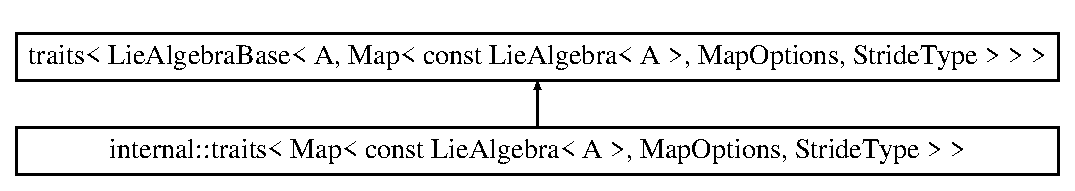
\includegraphics[height=2.000000cm]{structinternal_1_1traits_3_01_map_3_01const_01_lie_algebra_3_01_a_01_4_00_01_map_options_00_01_stride_type_01_4_01_4}
\end{center}
\end{figure}
\subsection*{Public Types}
\begin{DoxyCompactItemize}
\item 
typedef Map$<$ const A, Map\+Options, Stride\+Type $>$ \hyperlink{structinternal_1_1traits_3_01_map_3_01const_01_lie_algebra_3_01_a_01_4_00_01_map_options_00_01_stride_type_01_4_01_4_a674c3c33e67dbce98e62c32725b274da}{Coefficients}
\end{DoxyCompactItemize}


\subsection{Detailed Description}
\subsubsection*{template$<$class A, int Map\+Options, typename Stride\+Type$>$\newline
struct internal\+::traits$<$ Map$<$ const Lie\+Algebra$<$ A $>$, Map\+Options, Stride\+Type $>$ $>$}



Definition at line 256 of file Lie\+Algebra.\+h.



\subsection{Member Typedef Documentation}
\hypertarget{structinternal_1_1traits_3_01_map_3_01const_01_lie_algebra_3_01_a_01_4_00_01_map_options_00_01_stride_type_01_4_01_4_a674c3c33e67dbce98e62c32725b274da}{}\label{structinternal_1_1traits_3_01_map_3_01const_01_lie_algebra_3_01_a_01_4_00_01_map_options_00_01_stride_type_01_4_01_4_a674c3c33e67dbce98e62c32725b274da} 
\index{internal\+::traits$<$ Map$<$ const Lie\+Algebra$<$ A $>$, Map\+Options, Stride\+Type $>$ $>$@{internal\+::traits$<$ Map$<$ const Lie\+Algebra$<$ A $>$, Map\+Options, Stride\+Type $>$ $>$}!Coefficients@{Coefficients}}
\index{Coefficients@{Coefficients}!internal\+::traits$<$ Map$<$ const Lie\+Algebra$<$ A $>$, Map\+Options, Stride\+Type $>$ $>$@{internal\+::traits$<$ Map$<$ const Lie\+Algebra$<$ A $>$, Map\+Options, Stride\+Type $>$ $>$}}
\subsubsection{\texorpdfstring{Coefficients}{Coefficients}}
{\footnotesize\ttfamily template$<$class A , int Map\+Options, typename Stride\+Type $>$ \\
typedef Map$<$const A, Map\+Options, Stride\+Type$>$ internal\+::traits$<$ Map$<$ const \hyperlink{class_lie_algebra}{Lie\+Algebra}$<$ A $>$, Map\+Options, Stride\+Type $>$ $>$\+::\hyperlink{structinternal_1_1traits_3_01_map_3_01const_01_lie_algebra_3_01_a_01_4_00_01_map_options_00_01_stride_type_01_4_01_4_a674c3c33e67dbce98e62c32725b274da}{Coefficients}}



Definition at line 258 of file Lie\+Algebra.\+h.



The documentation for this struct was generated from the following file\+:\begin{DoxyCompactItemize}
\item 
/\+Users/\+Ryan/\+Code/codyco-\/superbuild/libraries/\+Eigen\+Lgsm/unsupported/\+Eigen/src/\+Lgsm/\hyperlink{_lie_algebra_8h}{Lie\+Algebra.\+h}\end{DoxyCompactItemize}

\hypertarget{structinternal_1_1traits_3_01_map_3_01const_01_lie_algebra_3_01_matrix_3_01_scalar_00_013_00_011480673ebb2de2c070cfdb8edee3d7437}{}\section{internal\+:\+:traits$<$ Map$<$ const Lie\+Algebra$<$ Matrix$<$ Scalar, 3, 1 $>$ $>$, Options $>$ $>$ Struct Template Reference}
\label{structinternal_1_1traits_3_01_map_3_01const_01_lie_algebra_3_01_matrix_3_01_scalar_00_013_00_011480673ebb2de2c070cfdb8edee3d7437}\index{internal\+::traits$<$ Map$<$ const Lie\+Algebra$<$ Matrix$<$ Scalar, 3, 1 $>$ $>$, Options $>$ $>$@{internal\+::traits$<$ Map$<$ const Lie\+Algebra$<$ Matrix$<$ Scalar, 3, 1 $>$ $>$, Options $>$ $>$}}


{\ttfamily \#include $<$Lie\+Algebra\+\_\+so3.\+h$>$}

Inheritance diagram for internal\+:\+:traits$<$ Map$<$ const Lie\+Algebra$<$ Matrix$<$ Scalar, 3, 1 $>$ $>$, Options $>$ $>$\+:\begin{figure}[H]
\begin{center}
\leavevmode
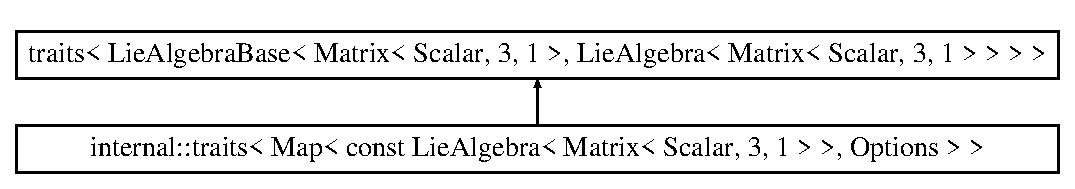
\includegraphics[height=2.000000cm]{structinternal_1_1traits_3_01_map_3_01const_01_lie_algebra_3_01_matrix_3_01_scalar_00_013_00_011480673ebb2de2c070cfdb8edee3d7437}
\end{center}
\end{figure}
\subsection*{Public Types}
\begin{DoxyCompactItemize}
\item 
typedef Map$<$ const Matrix$<$ Scalar, 3, 1 $>$, Options $>$ \hyperlink{structinternal_1_1traits_3_01_map_3_01const_01_lie_algebra_3_01_matrix_3_01_scalar_00_013_00_011480673ebb2de2c070cfdb8edee3d7437_abd106fedc67f9610cb2b8ee96ce8aa27}{Coefficients}
\item 
typedef \hyperlink{class_lie_group}{Lie\+Group}$<$ Quaternion$<$ Scalar $>$ $>$ \hyperlink{structinternal_1_1traits_3_01_map_3_01const_01_lie_algebra_3_01_matrix_3_01_scalar_00_013_00_011480673ebb2de2c070cfdb8edee3d7437_acdfb59027e942e113b4f8ad4defe78e0}{Group}
\end{DoxyCompactItemize}


\subsection{Detailed Description}
\subsubsection*{template$<$typename Scalar, int Options$>$\newline
struct internal\+::traits$<$ Map$<$ const Lie\+Algebra$<$ Matrix$<$ Scalar, 3, 1 $>$ $>$, Options $>$ $>$}



Definition at line 314 of file Lie\+Algebra\+\_\+so3.\+h.



\subsection{Member Typedef Documentation}
\hypertarget{structinternal_1_1traits_3_01_map_3_01const_01_lie_algebra_3_01_matrix_3_01_scalar_00_013_00_011480673ebb2de2c070cfdb8edee3d7437_abd106fedc67f9610cb2b8ee96ce8aa27}{}\label{structinternal_1_1traits_3_01_map_3_01const_01_lie_algebra_3_01_matrix_3_01_scalar_00_013_00_011480673ebb2de2c070cfdb8edee3d7437_abd106fedc67f9610cb2b8ee96ce8aa27} 
\index{internal\+::traits$<$ Map$<$ const Lie\+Algebra$<$ Matrix$<$ Scalar, 3, 1 $>$ $>$, Options $>$ $>$@{internal\+::traits$<$ Map$<$ const Lie\+Algebra$<$ Matrix$<$ Scalar, 3, 1 $>$ $>$, Options $>$ $>$}!Coefficients@{Coefficients}}
\index{Coefficients@{Coefficients}!internal\+::traits$<$ Map$<$ const Lie\+Algebra$<$ Matrix$<$ Scalar, 3, 1 $>$ $>$, Options $>$ $>$@{internal\+::traits$<$ Map$<$ const Lie\+Algebra$<$ Matrix$<$ Scalar, 3, 1 $>$ $>$, Options $>$ $>$}}
\subsubsection{\texorpdfstring{Coefficients}{Coefficients}}
{\footnotesize\ttfamily template$<$typename Scalar , int Options$>$ \\
typedef Map$<$const Matrix$<$Scalar, 3, 1$>$, Options$>$ internal\+::traits$<$ Map$<$ const \hyperlink{class_lie_algebra}{Lie\+Algebra}$<$ Matrix$<$ Scalar, 3, 1 $>$ $>$, Options $>$ $>$\+::\hyperlink{structinternal_1_1traits_3_01_map_3_01const_01_lie_algebra_3_01_matrix_3_01_scalar_00_013_00_011480673ebb2de2c070cfdb8edee3d7437_abd106fedc67f9610cb2b8ee96ce8aa27}{Coefficients}}



Definition at line 317 of file Lie\+Algebra\+\_\+so3.\+h.

\hypertarget{structinternal_1_1traits_3_01_map_3_01const_01_lie_algebra_3_01_matrix_3_01_scalar_00_013_00_011480673ebb2de2c070cfdb8edee3d7437_acdfb59027e942e113b4f8ad4defe78e0}{}\label{structinternal_1_1traits_3_01_map_3_01const_01_lie_algebra_3_01_matrix_3_01_scalar_00_013_00_011480673ebb2de2c070cfdb8edee3d7437_acdfb59027e942e113b4f8ad4defe78e0} 
\index{internal\+::traits$<$ Map$<$ const Lie\+Algebra$<$ Matrix$<$ Scalar, 3, 1 $>$ $>$, Options $>$ $>$@{internal\+::traits$<$ Map$<$ const Lie\+Algebra$<$ Matrix$<$ Scalar, 3, 1 $>$ $>$, Options $>$ $>$}!Group@{Group}}
\index{Group@{Group}!internal\+::traits$<$ Map$<$ const Lie\+Algebra$<$ Matrix$<$ Scalar, 3, 1 $>$ $>$, Options $>$ $>$@{internal\+::traits$<$ Map$<$ const Lie\+Algebra$<$ Matrix$<$ Scalar, 3, 1 $>$ $>$, Options $>$ $>$}}
\subsubsection{\texorpdfstring{Group}{Group}}
{\footnotesize\ttfamily template$<$typename Scalar , int Options$>$ \\
typedef \hyperlink{class_lie_group}{Lie\+Group}$<$Quaternion$<$Scalar$>$ $>$ internal\+::traits$<$ Map$<$ const \hyperlink{class_lie_algebra}{Lie\+Algebra}$<$ Matrix$<$ Scalar, 3, 1 $>$ $>$, Options $>$ $>$\+::\hyperlink{structinternal_1_1traits_3_01_map_3_01const_01_lie_algebra_3_01_matrix_3_01_scalar_00_013_00_011480673ebb2de2c070cfdb8edee3d7437_acdfb59027e942e113b4f8ad4defe78e0}{Group}}



Definition at line 318 of file Lie\+Algebra\+\_\+so3.\+h.



The documentation for this struct was generated from the following file\+:\begin{DoxyCompactItemize}
\item 
/\+Users/\+Ryan/\+Code/codyco-\/superbuild/libraries/\+Eigen\+Lgsm/unsupported/\+Eigen/src/\+Lgsm/\hyperlink{_lie_algebra__so3_8h}{Lie\+Algebra\+\_\+so3.\+h}\end{DoxyCompactItemize}

\hypertarget{structinternal_1_1traits_3_01_map_3_01const_01_lie_algebra_3_01_matrix_3_01_scalar_00_016_00_011bdc50eba447989365acf4f3cfd5e5212}{}\section{internal\+:\+:traits$<$ Map$<$ const Lie\+Algebra$<$ Matrix$<$ Scalar, 6, 1 $>$ $>$, Options $>$ $>$ Struct Template Reference}
\label{structinternal_1_1traits_3_01_map_3_01const_01_lie_algebra_3_01_matrix_3_01_scalar_00_016_00_011bdc50eba447989365acf4f3cfd5e5212}\index{internal\+::traits$<$ Map$<$ const Lie\+Algebra$<$ Matrix$<$ Scalar, 6, 1 $>$ $>$, Options $>$ $>$@{internal\+::traits$<$ Map$<$ const Lie\+Algebra$<$ Matrix$<$ Scalar, 6, 1 $>$ $>$, Options $>$ $>$}}


{\ttfamily \#include $<$Lie\+Algebra\+\_\+se3.\+h$>$}

Inheritance diagram for internal\+:\+:traits$<$ Map$<$ const Lie\+Algebra$<$ Matrix$<$ Scalar, 6, 1 $>$ $>$, Options $>$ $>$\+:\begin{figure}[H]
\begin{center}
\leavevmode
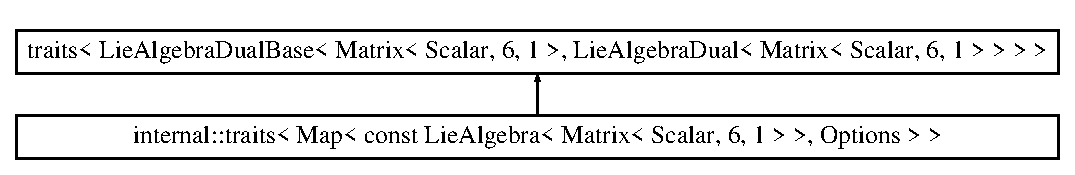
\includegraphics[height=1.904762cm]{structinternal_1_1traits_3_01_map_3_01const_01_lie_algebra_3_01_matrix_3_01_scalar_00_016_00_011bdc50eba447989365acf4f3cfd5e5212}
\end{center}
\end{figure}
\subsection*{Public Types}
\begin{DoxyCompactItemize}
\item 
typedef Map$<$ const Matrix$<$ Scalar, 6, 1 $>$, Options $>$ \hyperlink{structinternal_1_1traits_3_01_map_3_01const_01_lie_algebra_3_01_matrix_3_01_scalar_00_016_00_011bdc50eba447989365acf4f3cfd5e5212_a9f0719d8c0161f53a3026c0d98dffa53}{Coefficients}
\item 
typedef \hyperlink{class_lie_group}{Lie\+Group}$<$ Array$<$ Scalar, 7, 1 $>$ $>$ \hyperlink{structinternal_1_1traits_3_01_map_3_01const_01_lie_algebra_3_01_matrix_3_01_scalar_00_016_00_011bdc50eba447989365acf4f3cfd5e5212_affc6fce5ea66d7dd41c559a4a6cc8e0d}{Group}
\end{DoxyCompactItemize}


\subsection{Detailed Description}
\subsubsection*{template$<$typename Scalar, int Options$>$\newline
struct internal\+::traits$<$ Map$<$ const Lie\+Algebra$<$ Matrix$<$ Scalar, 6, 1 $>$ $>$, Options $>$ $>$}



Definition at line 256 of file Lie\+Algebra\+\_\+se3.\+h.



\subsection{Member Typedef Documentation}
\hypertarget{structinternal_1_1traits_3_01_map_3_01const_01_lie_algebra_3_01_matrix_3_01_scalar_00_016_00_011bdc50eba447989365acf4f3cfd5e5212_a9f0719d8c0161f53a3026c0d98dffa53}{}\label{structinternal_1_1traits_3_01_map_3_01const_01_lie_algebra_3_01_matrix_3_01_scalar_00_016_00_011bdc50eba447989365acf4f3cfd5e5212_a9f0719d8c0161f53a3026c0d98dffa53} 
\index{internal\+::traits$<$ Map$<$ const Lie\+Algebra$<$ Matrix$<$ Scalar, 6, 1 $>$ $>$, Options $>$ $>$@{internal\+::traits$<$ Map$<$ const Lie\+Algebra$<$ Matrix$<$ Scalar, 6, 1 $>$ $>$, Options $>$ $>$}!Coefficients@{Coefficients}}
\index{Coefficients@{Coefficients}!internal\+::traits$<$ Map$<$ const Lie\+Algebra$<$ Matrix$<$ Scalar, 6, 1 $>$ $>$, Options $>$ $>$@{internal\+::traits$<$ Map$<$ const Lie\+Algebra$<$ Matrix$<$ Scalar, 6, 1 $>$ $>$, Options $>$ $>$}}
\subsubsection{\texorpdfstring{Coefficients}{Coefficients}}
{\footnotesize\ttfamily template$<$typename Scalar , int Options$>$ \\
typedef Map$<$const Matrix$<$Scalar, 6, 1$>$, Options$>$ internal\+::traits$<$ Map$<$ const \hyperlink{class_lie_algebra}{Lie\+Algebra}$<$ Matrix$<$ Scalar, 6, 1 $>$ $>$, Options $>$ $>$\+::\hyperlink{structinternal_1_1traits_3_01_map_3_01const_01_lie_algebra_3_01_matrix_3_01_scalar_00_016_00_011bdc50eba447989365acf4f3cfd5e5212_a9f0719d8c0161f53a3026c0d98dffa53}{Coefficients}}



Definition at line 259 of file Lie\+Algebra\+\_\+se3.\+h.

\hypertarget{structinternal_1_1traits_3_01_map_3_01const_01_lie_algebra_3_01_matrix_3_01_scalar_00_016_00_011bdc50eba447989365acf4f3cfd5e5212_affc6fce5ea66d7dd41c559a4a6cc8e0d}{}\label{structinternal_1_1traits_3_01_map_3_01const_01_lie_algebra_3_01_matrix_3_01_scalar_00_016_00_011bdc50eba447989365acf4f3cfd5e5212_affc6fce5ea66d7dd41c559a4a6cc8e0d} 
\index{internal\+::traits$<$ Map$<$ const Lie\+Algebra$<$ Matrix$<$ Scalar, 6, 1 $>$ $>$, Options $>$ $>$@{internal\+::traits$<$ Map$<$ const Lie\+Algebra$<$ Matrix$<$ Scalar, 6, 1 $>$ $>$, Options $>$ $>$}!Group@{Group}}
\index{Group@{Group}!internal\+::traits$<$ Map$<$ const Lie\+Algebra$<$ Matrix$<$ Scalar, 6, 1 $>$ $>$, Options $>$ $>$@{internal\+::traits$<$ Map$<$ const Lie\+Algebra$<$ Matrix$<$ Scalar, 6, 1 $>$ $>$, Options $>$ $>$}}
\subsubsection{\texorpdfstring{Group}{Group}}
{\footnotesize\ttfamily template$<$typename Scalar , int Options$>$ \\
typedef \hyperlink{class_lie_group}{Lie\+Group}$<$Array$<$Scalar, 7, 1$>$ $>$ internal\+::traits$<$ Map$<$ const \hyperlink{class_lie_algebra}{Lie\+Algebra}$<$ Matrix$<$ Scalar, 6, 1 $>$ $>$, Options $>$ $>$\+::\hyperlink{structinternal_1_1traits_3_01_map_3_01const_01_lie_algebra_3_01_matrix_3_01_scalar_00_016_00_011bdc50eba447989365acf4f3cfd5e5212_affc6fce5ea66d7dd41c559a4a6cc8e0d}{Group}}



Definition at line 260 of file Lie\+Algebra\+\_\+se3.\+h.



The documentation for this struct was generated from the following file\+:\begin{DoxyCompactItemize}
\item 
/\+Users/\+Ryan/\+Code/codyco-\/superbuild/libraries/\+Eigen\+Lgsm/unsupported/\+Eigen/src/\+Lgsm/\hyperlink{_lie_algebra__se3_8h}{Lie\+Algebra\+\_\+se3.\+h}\end{DoxyCompactItemize}

\hypertarget{structinternal_1_1traits_3_01_map_3_01const_01_lie_algebra_dual_3_01_a_01_4_00_01_map_options_00_01_stride_type_01_4_01_4}{}\section{internal\+:\+:traits$<$ Map$<$ const Lie\+Algebra\+Dual$<$ A $>$, Map\+Options, Stride\+Type $>$ $>$ Struct Template Reference}
\label{structinternal_1_1traits_3_01_map_3_01const_01_lie_algebra_dual_3_01_a_01_4_00_01_map_options_00_01_stride_type_01_4_01_4}\index{internal\+::traits$<$ Map$<$ const Lie\+Algebra\+Dual$<$ A $>$, Map\+Options, Stride\+Type $>$ $>$@{internal\+::traits$<$ Map$<$ const Lie\+Algebra\+Dual$<$ A $>$, Map\+Options, Stride\+Type $>$ $>$}}


{\ttfamily \#include $<$Lie\+Algebra.\+h$>$}

Inheritance diagram for internal\+:\+:traits$<$ Map$<$ const Lie\+Algebra\+Dual$<$ A $>$, Map\+Options, Stride\+Type $>$ $>$\+:\begin{figure}[H]
\begin{center}
\leavevmode
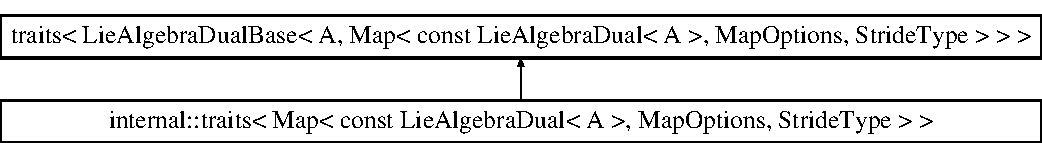
\includegraphics[height=1.927711cm]{structinternal_1_1traits_3_01_map_3_01const_01_lie_algebra_dual_3_01_a_01_4_00_01_map_options_00_01_stride_type_01_4_01_4}
\end{center}
\end{figure}
\subsection*{Public Types}
\begin{DoxyCompactItemize}
\item 
typedef Map$<$ A, Map\+Options, Stride\+Type $>$ \hyperlink{structinternal_1_1traits_3_01_map_3_01const_01_lie_algebra_dual_3_01_a_01_4_00_01_map_options_00_01_stride_type_01_4_01_4_a459b9a329ae5a1cbe01f3e0456c6eb70}{Coefficients}
\end{DoxyCompactItemize}


\subsection{Detailed Description}
\subsubsection*{template$<$class A, int Map\+Options, typename Stride\+Type$>$\newline
struct internal\+::traits$<$ Map$<$ const Lie\+Algebra\+Dual$<$ A $>$, Map\+Options, Stride\+Type $>$ $>$}



Definition at line 349 of file Lie\+Algebra.\+h.



\subsection{Member Typedef Documentation}
\hypertarget{structinternal_1_1traits_3_01_map_3_01const_01_lie_algebra_dual_3_01_a_01_4_00_01_map_options_00_01_stride_type_01_4_01_4_a459b9a329ae5a1cbe01f3e0456c6eb70}{}\label{structinternal_1_1traits_3_01_map_3_01const_01_lie_algebra_dual_3_01_a_01_4_00_01_map_options_00_01_stride_type_01_4_01_4_a459b9a329ae5a1cbe01f3e0456c6eb70} 
\index{internal\+::traits$<$ Map$<$ const Lie\+Algebra\+Dual$<$ A $>$, Map\+Options, Stride\+Type $>$ $>$@{internal\+::traits$<$ Map$<$ const Lie\+Algebra\+Dual$<$ A $>$, Map\+Options, Stride\+Type $>$ $>$}!Coefficients@{Coefficients}}
\index{Coefficients@{Coefficients}!internal\+::traits$<$ Map$<$ const Lie\+Algebra\+Dual$<$ A $>$, Map\+Options, Stride\+Type $>$ $>$@{internal\+::traits$<$ Map$<$ const Lie\+Algebra\+Dual$<$ A $>$, Map\+Options, Stride\+Type $>$ $>$}}
\subsubsection{\texorpdfstring{Coefficients}{Coefficients}}
{\footnotesize\ttfamily template$<$class A , int Map\+Options, typename Stride\+Type $>$ \\
typedef Map$<$A, Map\+Options, Stride\+Type$>$ internal\+::traits$<$ Map$<$ const \hyperlink{class_lie_algebra_dual}{Lie\+Algebra\+Dual}$<$ A $>$, Map\+Options, Stride\+Type $>$ $>$\+::\hyperlink{structinternal_1_1traits_3_01_map_3_01const_01_lie_algebra_dual_3_01_a_01_4_00_01_map_options_00_01_stride_type_01_4_01_4_a459b9a329ae5a1cbe01f3e0456c6eb70}{Coefficients}}



Definition at line 351 of file Lie\+Algebra.\+h.



The documentation for this struct was generated from the following file\+:\begin{DoxyCompactItemize}
\item 
/\+Users/\+Ryan/\+Code/codyco-\/superbuild/libraries/\+Eigen\+Lgsm/unsupported/\+Eigen/src/\+Lgsm/\hyperlink{_lie_algebra_8h}{Lie\+Algebra.\+h}\end{DoxyCompactItemize}

\hypertarget{structinternal_1_1traits_3_01_map_3_01const_01_lie_algebra_dual_3_01_matrix_3_01_scalar_00_013_0e77a233aa7e2f28dddf71e39df1dd866}{}\section{internal\+:\+:traits$<$ Map$<$ const Lie\+Algebra\+Dual$<$ Matrix$<$ Scalar, 3, 1 $>$ $>$, Map\+Options $>$ $>$ Struct Template Reference}
\label{structinternal_1_1traits_3_01_map_3_01const_01_lie_algebra_dual_3_01_matrix_3_01_scalar_00_013_0e77a233aa7e2f28dddf71e39df1dd866}\index{internal\+::traits$<$ Map$<$ const Lie\+Algebra\+Dual$<$ Matrix$<$ Scalar, 3, 1 $>$ $>$, Map\+Options $>$ $>$@{internal\+::traits$<$ Map$<$ const Lie\+Algebra\+Dual$<$ Matrix$<$ Scalar, 3, 1 $>$ $>$, Map\+Options $>$ $>$}}


{\ttfamily \#include $<$Lie\+Algebra\+\_\+so3.\+h$>$}

Inheritance diagram for internal\+:\+:traits$<$ Map$<$ const Lie\+Algebra\+Dual$<$ Matrix$<$ Scalar, 3, 1 $>$ $>$, Map\+Options $>$ $>$\+:\begin{figure}[H]
\begin{center}
\leavevmode
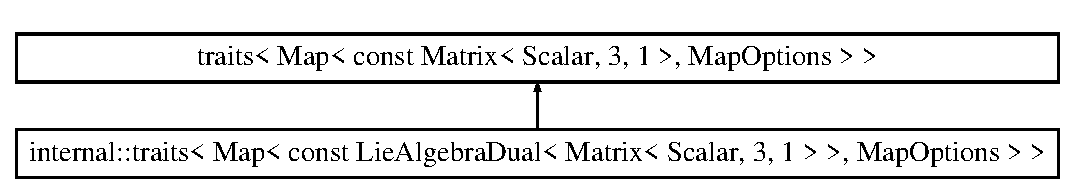
\includegraphics[height=2.000000cm]{structinternal_1_1traits_3_01_map_3_01const_01_lie_algebra_dual_3_01_matrix_3_01_scalar_00_013_0e77a233aa7e2f28dddf71e39df1dd866}
\end{center}
\end{figure}
\subsection*{Public Types}
\begin{DoxyCompactItemize}
\item 
typedef Map$<$ const Matrix$<$ Scalar, 3, 1 $>$, Map\+Options $>$ \hyperlink{structinternal_1_1traits_3_01_map_3_01const_01_lie_algebra_dual_3_01_matrix_3_01_scalar_00_013_0e77a233aa7e2f28dddf71e39df1dd866_a925f17123c9a6154ed57fa5c397780cd}{Coefficients}
\item 
typedef \hyperlink{class_lie_group}{Lie\+Group}$<$ Quaternion$<$ Scalar $>$ $>$ \hyperlink{structinternal_1_1traits_3_01_map_3_01const_01_lie_algebra_dual_3_01_matrix_3_01_scalar_00_013_0e77a233aa7e2f28dddf71e39df1dd866_af93405032a1b0062e9c3ca662f0cfcbe}{Group}
\end{DoxyCompactItemize}


\subsection{Detailed Description}
\subsubsection*{template$<$typename Scalar, int Map\+Options$>$\newline
struct internal\+::traits$<$ Map$<$ const Lie\+Algebra\+Dual$<$ Matrix$<$ Scalar, 3, 1 $>$ $>$, Map\+Options $>$ $>$}



Definition at line 272 of file Lie\+Algebra\+\_\+so3.\+h.



\subsection{Member Typedef Documentation}
\hypertarget{structinternal_1_1traits_3_01_map_3_01const_01_lie_algebra_dual_3_01_matrix_3_01_scalar_00_013_0e77a233aa7e2f28dddf71e39df1dd866_a925f17123c9a6154ed57fa5c397780cd}{}\label{structinternal_1_1traits_3_01_map_3_01const_01_lie_algebra_dual_3_01_matrix_3_01_scalar_00_013_0e77a233aa7e2f28dddf71e39df1dd866_a925f17123c9a6154ed57fa5c397780cd} 
\index{internal\+::traits$<$ Map$<$ const Lie\+Algebra\+Dual$<$ Matrix$<$ Scalar, 3, 1 $>$ $>$, Map\+Options $>$ $>$@{internal\+::traits$<$ Map$<$ const Lie\+Algebra\+Dual$<$ Matrix$<$ Scalar, 3, 1 $>$ $>$, Map\+Options $>$ $>$}!Coefficients@{Coefficients}}
\index{Coefficients@{Coefficients}!internal\+::traits$<$ Map$<$ const Lie\+Algebra\+Dual$<$ Matrix$<$ Scalar, 3, 1 $>$ $>$, Map\+Options $>$ $>$@{internal\+::traits$<$ Map$<$ const Lie\+Algebra\+Dual$<$ Matrix$<$ Scalar, 3, 1 $>$ $>$, Map\+Options $>$ $>$}}
\subsubsection{\texorpdfstring{Coefficients}{Coefficients}}
{\footnotesize\ttfamily template$<$typename Scalar , int Map\+Options$>$ \\
typedef Map$<$const Matrix$<$Scalar, 3, 1$>$, Map\+Options$>$ internal\+::traits$<$ Map$<$ const \hyperlink{class_lie_algebra_dual}{Lie\+Algebra\+Dual}$<$ Matrix$<$ Scalar, 3, 1 $>$ $>$, Map\+Options $>$ $>$\+::\hyperlink{structinternal_1_1traits_3_01_map_3_01const_01_lie_algebra_dual_3_01_matrix_3_01_scalar_00_013_0e77a233aa7e2f28dddf71e39df1dd866_a925f17123c9a6154ed57fa5c397780cd}{Coefficients}}



Definition at line 274 of file Lie\+Algebra\+\_\+so3.\+h.

\hypertarget{structinternal_1_1traits_3_01_map_3_01const_01_lie_algebra_dual_3_01_matrix_3_01_scalar_00_013_0e77a233aa7e2f28dddf71e39df1dd866_af93405032a1b0062e9c3ca662f0cfcbe}{}\label{structinternal_1_1traits_3_01_map_3_01const_01_lie_algebra_dual_3_01_matrix_3_01_scalar_00_013_0e77a233aa7e2f28dddf71e39df1dd866_af93405032a1b0062e9c3ca662f0cfcbe} 
\index{internal\+::traits$<$ Map$<$ const Lie\+Algebra\+Dual$<$ Matrix$<$ Scalar, 3, 1 $>$ $>$, Map\+Options $>$ $>$@{internal\+::traits$<$ Map$<$ const Lie\+Algebra\+Dual$<$ Matrix$<$ Scalar, 3, 1 $>$ $>$, Map\+Options $>$ $>$}!Group@{Group}}
\index{Group@{Group}!internal\+::traits$<$ Map$<$ const Lie\+Algebra\+Dual$<$ Matrix$<$ Scalar, 3, 1 $>$ $>$, Map\+Options $>$ $>$@{internal\+::traits$<$ Map$<$ const Lie\+Algebra\+Dual$<$ Matrix$<$ Scalar, 3, 1 $>$ $>$, Map\+Options $>$ $>$}}
\subsubsection{\texorpdfstring{Group}{Group}}
{\footnotesize\ttfamily template$<$typename Scalar , int Map\+Options$>$ \\
typedef \hyperlink{class_lie_group}{Lie\+Group}$<$Quaternion$<$Scalar$>$ $>$ internal\+::traits$<$ Map$<$ const \hyperlink{class_lie_algebra_dual}{Lie\+Algebra\+Dual}$<$ Matrix$<$ Scalar, 3, 1 $>$ $>$, Map\+Options $>$ $>$\+::\hyperlink{structinternal_1_1traits_3_01_map_3_01const_01_lie_algebra_dual_3_01_matrix_3_01_scalar_00_013_0e77a233aa7e2f28dddf71e39df1dd866_af93405032a1b0062e9c3ca662f0cfcbe}{Group}}



Definition at line 275 of file Lie\+Algebra\+\_\+so3.\+h.



The documentation for this struct was generated from the following file\+:\begin{DoxyCompactItemize}
\item 
/\+Users/\+Ryan/\+Code/codyco-\/superbuild/libraries/\+Eigen\+Lgsm/unsupported/\+Eigen/src/\+Lgsm/\hyperlink{_lie_algebra__so3_8h}{Lie\+Algebra\+\_\+so3.\+h}\end{DoxyCompactItemize}

\hypertarget{structinternal_1_1traits_3_01_map_3_01const_01_lie_group_3_01_g_01_4_00_01_map_options_00_01_stride_type_01_4_01_4}{}\section{internal\+:\+:traits$<$ Map$<$ const Lie\+Group$<$ G $>$, Map\+Options, Stride\+Type $>$ $>$ Struct Template Reference}
\label{structinternal_1_1traits_3_01_map_3_01const_01_lie_group_3_01_g_01_4_00_01_map_options_00_01_stride_type_01_4_01_4}\index{internal\+::traits$<$ Map$<$ const Lie\+Group$<$ G $>$, Map\+Options, Stride\+Type $>$ $>$@{internal\+::traits$<$ Map$<$ const Lie\+Group$<$ G $>$, Map\+Options, Stride\+Type $>$ $>$}}


{\ttfamily \#include $<$Lie\+Group.\+h$>$}

Inheritance diagram for internal\+:\+:traits$<$ Map$<$ const Lie\+Group$<$ G $>$, Map\+Options, Stride\+Type $>$ $>$\+:\begin{figure}[H]
\begin{center}
\leavevmode
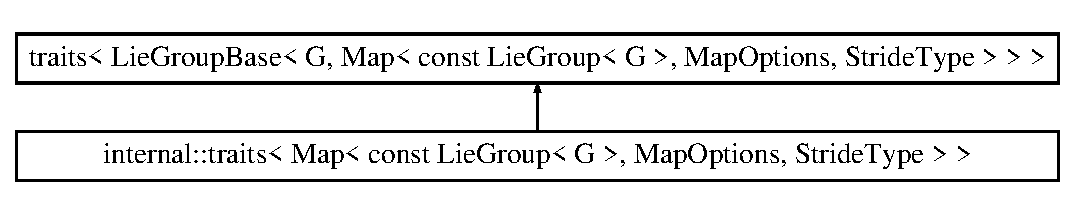
\includegraphics[height=2.000000cm]{structinternal_1_1traits_3_01_map_3_01const_01_lie_group_3_01_g_01_4_00_01_map_options_00_01_stride_type_01_4_01_4}
\end{center}
\end{figure}
\subsection*{Public Types}
\begin{DoxyCompactItemize}
\item 
typedef Map$<$ const G, Map\+Options, Stride\+Type $>$ \hyperlink{structinternal_1_1traits_3_01_map_3_01const_01_lie_group_3_01_g_01_4_00_01_map_options_00_01_stride_type_01_4_01_4_a8a1d9201a1ced7406d87434e78a1bb94}{Coefficients}
\item 
typedef G\+::\+Scalar \hyperlink{structinternal_1_1traits_3_01_map_3_01const_01_lie_group_3_01_g_01_4_00_01_map_options_00_01_stride_type_01_4_01_4_a3aab625ff94db50623851510a4420ab0}{Scalar}
\end{DoxyCompactItemize}


\subsection{Detailed Description}
\subsubsection*{template$<$class G, int Map\+Options, typename Stride\+Type$>$\newline
struct internal\+::traits$<$ Map$<$ const Lie\+Group$<$ G $>$, Map\+Options, Stride\+Type $>$ $>$}



Definition at line 157 of file Lie\+Group.\+h.



\subsection{Member Typedef Documentation}
\hypertarget{structinternal_1_1traits_3_01_map_3_01const_01_lie_group_3_01_g_01_4_00_01_map_options_00_01_stride_type_01_4_01_4_a8a1d9201a1ced7406d87434e78a1bb94}{}\label{structinternal_1_1traits_3_01_map_3_01const_01_lie_group_3_01_g_01_4_00_01_map_options_00_01_stride_type_01_4_01_4_a8a1d9201a1ced7406d87434e78a1bb94} 
\index{internal\+::traits$<$ Map$<$ const Lie\+Group$<$ G $>$, Map\+Options, Stride\+Type $>$ $>$@{internal\+::traits$<$ Map$<$ const Lie\+Group$<$ G $>$, Map\+Options, Stride\+Type $>$ $>$}!Coefficients@{Coefficients}}
\index{Coefficients@{Coefficients}!internal\+::traits$<$ Map$<$ const Lie\+Group$<$ G $>$, Map\+Options, Stride\+Type $>$ $>$@{internal\+::traits$<$ Map$<$ const Lie\+Group$<$ G $>$, Map\+Options, Stride\+Type $>$ $>$}}
\subsubsection{\texorpdfstring{Coefficients}{Coefficients}}
{\footnotesize\ttfamily template$<$class G , int Map\+Options, typename Stride\+Type $>$ \\
typedef Map$<$const G, Map\+Options, Stride\+Type$>$ internal\+::traits$<$ Map$<$ const \hyperlink{class_lie_group}{Lie\+Group}$<$ G $>$, Map\+Options, Stride\+Type $>$ $>$\+::\hyperlink{structinternal_1_1traits_3_01_map_3_01const_01_lie_group_3_01_g_01_4_00_01_map_options_00_01_stride_type_01_4_01_4_a8a1d9201a1ced7406d87434e78a1bb94}{Coefficients}}



Definition at line 159 of file Lie\+Group.\+h.

\hypertarget{structinternal_1_1traits_3_01_map_3_01const_01_lie_group_3_01_g_01_4_00_01_map_options_00_01_stride_type_01_4_01_4_a3aab625ff94db50623851510a4420ab0}{}\label{structinternal_1_1traits_3_01_map_3_01const_01_lie_group_3_01_g_01_4_00_01_map_options_00_01_stride_type_01_4_01_4_a3aab625ff94db50623851510a4420ab0} 
\index{internal\+::traits$<$ Map$<$ const Lie\+Group$<$ G $>$, Map\+Options, Stride\+Type $>$ $>$@{internal\+::traits$<$ Map$<$ const Lie\+Group$<$ G $>$, Map\+Options, Stride\+Type $>$ $>$}!Scalar@{Scalar}}
\index{Scalar@{Scalar}!internal\+::traits$<$ Map$<$ const Lie\+Group$<$ G $>$, Map\+Options, Stride\+Type $>$ $>$@{internal\+::traits$<$ Map$<$ const Lie\+Group$<$ G $>$, Map\+Options, Stride\+Type $>$ $>$}}
\subsubsection{\texorpdfstring{Scalar}{Scalar}}
{\footnotesize\ttfamily template$<$class G , int Map\+Options, typename Stride\+Type $>$ \\
typedef G\+::\+Scalar internal\+::traits$<$ Map$<$ const \hyperlink{class_lie_group}{Lie\+Group}$<$ G $>$, Map\+Options, Stride\+Type $>$ $>$\+::\hyperlink{structinternal_1_1traits_3_01_map_3_01const_01_lie_group_3_01_g_01_4_00_01_map_options_00_01_stride_type_01_4_01_4_a3aab625ff94db50623851510a4420ab0}{Scalar}}



Definition at line 160 of file Lie\+Group.\+h.



The documentation for this struct was generated from the following file\+:\begin{DoxyCompactItemize}
\item 
/\+Users/\+Ryan/\+Code/codyco-\/superbuild/libraries/\+Eigen\+Lgsm/unsupported/\+Eigen/src/\+Lgsm/\hyperlink{_lie_group_8h}{Lie\+Group.\+h}\end{DoxyCompactItemize}

\hypertarget{structinternal_1_1traits_3_01_map_3_01_displacement_3_01___scalar_01_4_00_01_map_options_00_01_stride_type_01_4_01_4}{}\section{internal\+:\+:traits$<$ Map$<$ Displacement$<$ \+\_\+\+Scalar $>$, Map\+Options, Stride\+Type $>$ $>$ Struct Template Reference}
\label{structinternal_1_1traits_3_01_map_3_01_displacement_3_01___scalar_01_4_00_01_map_options_00_01_stride_type_01_4_01_4}\index{internal\+::traits$<$ Map$<$ Displacement$<$ \+\_\+\+Scalar $>$, Map\+Options, Stride\+Type $>$ $>$@{internal\+::traits$<$ Map$<$ Displacement$<$ \+\_\+\+Scalar $>$, Map\+Options, Stride\+Type $>$ $>$}}


{\ttfamily \#include $<$Displacement.\+h$>$}

Inheritance diagram for internal\+:\+:traits$<$ Map$<$ Displacement$<$ \+\_\+\+Scalar $>$, Map\+Options, Stride\+Type $>$ $>$\+:\begin{figure}[H]
\begin{center}
\leavevmode
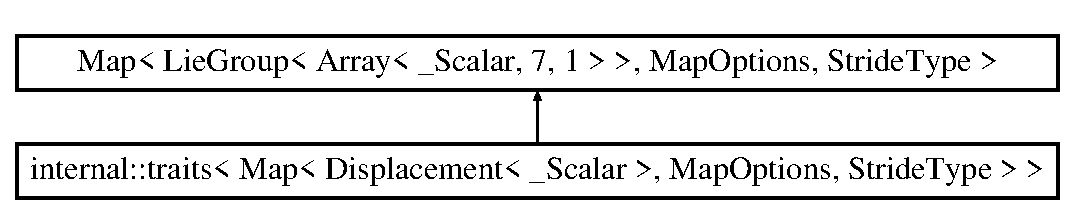
\includegraphics[height=2.000000cm]{structinternal_1_1traits_3_01_map_3_01_displacement_3_01___scalar_01_4_00_01_map_options_00_01_stride_type_01_4_01_4}
\end{center}
\end{figure}
\subsection*{Public Types}
\begin{DoxyCompactItemize}
\item 
typedef \hyperlink{class_displacement}{Displacement}$<$ \+\_\+\+Scalar $>$ \hyperlink{structinternal_1_1traits_3_01_map_3_01_displacement_3_01___scalar_01_4_00_01_map_options_00_01_stride_type_01_4_01_4_a731702958c8fe6e17c7ecfa15d75e5d0}{Plain\+Object}
\item 
typedef \+\_\+\+Scalar \hyperlink{structinternal_1_1traits_3_01_map_3_01_displacement_3_01___scalar_01_4_00_01_map_options_00_01_stride_type_01_4_01_4_af622b2eb414fa4600a591d0b6ae51f8d}{Scalar}
\end{DoxyCompactItemize}


\subsection{Detailed Description}
\subsubsection*{template$<$typename \+\_\+\+Scalar, int Map\+Options, typename Stride\+Type$>$\newline
struct internal\+::traits$<$ Map$<$ Displacement$<$ \+\_\+\+Scalar $>$, Map\+Options, Stride\+Type $>$ $>$}



Definition at line 229 of file Displacement.\+h.



\subsection{Member Typedef Documentation}
\hypertarget{structinternal_1_1traits_3_01_map_3_01_displacement_3_01___scalar_01_4_00_01_map_options_00_01_stride_type_01_4_01_4_a731702958c8fe6e17c7ecfa15d75e5d0}{}\label{structinternal_1_1traits_3_01_map_3_01_displacement_3_01___scalar_01_4_00_01_map_options_00_01_stride_type_01_4_01_4_a731702958c8fe6e17c7ecfa15d75e5d0} 
\index{internal\+::traits$<$ Map$<$ Displacement$<$ \+\_\+\+Scalar $>$, Map\+Options, Stride\+Type $>$ $>$@{internal\+::traits$<$ Map$<$ Displacement$<$ \+\_\+\+Scalar $>$, Map\+Options, Stride\+Type $>$ $>$}!Plain\+Object@{Plain\+Object}}
\index{Plain\+Object@{Plain\+Object}!internal\+::traits$<$ Map$<$ Displacement$<$ \+\_\+\+Scalar $>$, Map\+Options, Stride\+Type $>$ $>$@{internal\+::traits$<$ Map$<$ Displacement$<$ \+\_\+\+Scalar $>$, Map\+Options, Stride\+Type $>$ $>$}}
\subsubsection{\texorpdfstring{Plain\+Object}{PlainObject}}
{\footnotesize\ttfamily template$<$typename \+\_\+\+Scalar , int Map\+Options, typename Stride\+Type $>$ \\
typedef \hyperlink{class_displacement}{Displacement}$<$\+\_\+\+Scalar$>$ internal\+::traits$<$ Map$<$ \hyperlink{class_displacement}{Displacement}$<$ \+\_\+\+Scalar $>$, Map\+Options, Stride\+Type $>$ $>$\+::\hyperlink{structinternal_1_1traits_3_01_map_3_01_displacement_3_01___scalar_01_4_00_01_map_options_00_01_stride_type_01_4_01_4_a731702958c8fe6e17c7ecfa15d75e5d0}{Plain\+Object}}



Definition at line 231 of file Displacement.\+h.

\hypertarget{structinternal_1_1traits_3_01_map_3_01_displacement_3_01___scalar_01_4_00_01_map_options_00_01_stride_type_01_4_01_4_af622b2eb414fa4600a591d0b6ae51f8d}{}\label{structinternal_1_1traits_3_01_map_3_01_displacement_3_01___scalar_01_4_00_01_map_options_00_01_stride_type_01_4_01_4_af622b2eb414fa4600a591d0b6ae51f8d} 
\index{internal\+::traits$<$ Map$<$ Displacement$<$ \+\_\+\+Scalar $>$, Map\+Options, Stride\+Type $>$ $>$@{internal\+::traits$<$ Map$<$ Displacement$<$ \+\_\+\+Scalar $>$, Map\+Options, Stride\+Type $>$ $>$}!Scalar@{Scalar}}
\index{Scalar@{Scalar}!internal\+::traits$<$ Map$<$ Displacement$<$ \+\_\+\+Scalar $>$, Map\+Options, Stride\+Type $>$ $>$@{internal\+::traits$<$ Map$<$ Displacement$<$ \+\_\+\+Scalar $>$, Map\+Options, Stride\+Type $>$ $>$}}
\subsubsection{\texorpdfstring{Scalar}{Scalar}}
{\footnotesize\ttfamily template$<$typename \+\_\+\+Scalar , int Map\+Options, typename Stride\+Type $>$ \\
typedef \+\_\+\+Scalar internal\+::traits$<$ Map$<$ \hyperlink{class_displacement}{Displacement}$<$ \+\_\+\+Scalar $>$, Map\+Options, Stride\+Type $>$ $>$\+::\hyperlink{structinternal_1_1traits_3_01_map_3_01_displacement_3_01___scalar_01_4_00_01_map_options_00_01_stride_type_01_4_01_4_af622b2eb414fa4600a591d0b6ae51f8d}{Scalar}}



Definition at line 232 of file Displacement.\+h.



The documentation for this struct was generated from the following file\+:\begin{DoxyCompactItemize}
\item 
/\+Users/\+Ryan/\+Code/codyco-\/superbuild/libraries/\+Eigen\+Lgsm/unsupported/\+Eigen/src/\+Lgsm/\hyperlink{_displacement_8h}{Displacement.\+h}\end{DoxyCompactItemize}

\hypertarget{structinternal_1_1traits_3_01_map_3_01_lie_algebra_3_01_a_01_4_00_01_map_options_00_01_stride_type_01_4_01_4}{}\section{internal\+:\+:traits$<$ Map$<$ Lie\+Algebra$<$ A $>$, Map\+Options, Stride\+Type $>$ $>$ Struct Template Reference}
\label{structinternal_1_1traits_3_01_map_3_01_lie_algebra_3_01_a_01_4_00_01_map_options_00_01_stride_type_01_4_01_4}\index{internal\+::traits$<$ Map$<$ Lie\+Algebra$<$ A $>$, Map\+Options, Stride\+Type $>$ $>$@{internal\+::traits$<$ Map$<$ Lie\+Algebra$<$ A $>$, Map\+Options, Stride\+Type $>$ $>$}}


{\ttfamily \#include $<$Lie\+Algebra.\+h$>$}

Inheritance diagram for internal\+:\+:traits$<$ Map$<$ Lie\+Algebra$<$ A $>$, Map\+Options, Stride\+Type $>$ $>$\+:\begin{figure}[H]
\begin{center}
\leavevmode
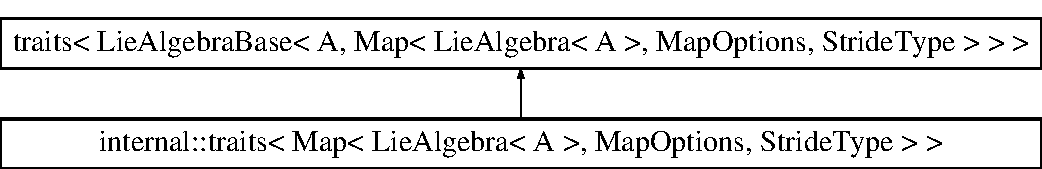
\includegraphics[height=2.000000cm]{structinternal_1_1traits_3_01_map_3_01_lie_algebra_3_01_a_01_4_00_01_map_options_00_01_stride_type_01_4_01_4}
\end{center}
\end{figure}
\subsection*{Public Types}
\begin{DoxyCompactItemize}
\item 
typedef Map$<$ A, Map\+Options, Stride\+Type $>$ \hyperlink{structinternal_1_1traits_3_01_map_3_01_lie_algebra_3_01_a_01_4_00_01_map_options_00_01_stride_type_01_4_01_4_a6d5295753fd15f374127373bcab1e504}{Coefficients}
\end{DoxyCompactItemize}


\subsection{Detailed Description}
\subsubsection*{template$<$class A, int Map\+Options, typename Stride\+Type$>$\newline
struct internal\+::traits$<$ Map$<$ Lie\+Algebra$<$ A $>$, Map\+Options, Stride\+Type $>$ $>$}



Definition at line 248 of file Lie\+Algebra.\+h.



\subsection{Member Typedef Documentation}
\hypertarget{structinternal_1_1traits_3_01_map_3_01_lie_algebra_3_01_a_01_4_00_01_map_options_00_01_stride_type_01_4_01_4_a6d5295753fd15f374127373bcab1e504}{}\label{structinternal_1_1traits_3_01_map_3_01_lie_algebra_3_01_a_01_4_00_01_map_options_00_01_stride_type_01_4_01_4_a6d5295753fd15f374127373bcab1e504} 
\index{internal\+::traits$<$ Map$<$ Lie\+Algebra$<$ A $>$, Map\+Options, Stride\+Type $>$ $>$@{internal\+::traits$<$ Map$<$ Lie\+Algebra$<$ A $>$, Map\+Options, Stride\+Type $>$ $>$}!Coefficients@{Coefficients}}
\index{Coefficients@{Coefficients}!internal\+::traits$<$ Map$<$ Lie\+Algebra$<$ A $>$, Map\+Options, Stride\+Type $>$ $>$@{internal\+::traits$<$ Map$<$ Lie\+Algebra$<$ A $>$, Map\+Options, Stride\+Type $>$ $>$}}
\subsubsection{\texorpdfstring{Coefficients}{Coefficients}}
{\footnotesize\ttfamily template$<$class A , int Map\+Options, typename Stride\+Type $>$ \\
typedef Map$<$A, Map\+Options, Stride\+Type$>$ internal\+::traits$<$ Map$<$ \hyperlink{class_lie_algebra}{Lie\+Algebra}$<$ A $>$, Map\+Options, Stride\+Type $>$ $>$\+::\hyperlink{structinternal_1_1traits_3_01_map_3_01_lie_algebra_3_01_a_01_4_00_01_map_options_00_01_stride_type_01_4_01_4_a6d5295753fd15f374127373bcab1e504}{Coefficients}}



Definition at line 250 of file Lie\+Algebra.\+h.



The documentation for this struct was generated from the following file\+:\begin{DoxyCompactItemize}
\item 
/\+Users/\+Ryan/\+Code/codyco-\/superbuild/libraries/\+Eigen\+Lgsm/unsupported/\+Eigen/src/\+Lgsm/\hyperlink{_lie_algebra_8h}{Lie\+Algebra.\+h}\end{DoxyCompactItemize}

\hypertarget{structinternal_1_1traits_3_01_map_3_01_lie_algebra_3_01_matrix_3_01_scalar_00_013_00_011_01_4_01_4_00_01_options_01_4_01_4}{}\section{internal\+:\+:traits$<$ Map$<$ Lie\+Algebra$<$ Matrix$<$ Scalar, 3, 1 $>$ $>$, Options $>$ $>$ Struct Template Reference}
\label{structinternal_1_1traits_3_01_map_3_01_lie_algebra_3_01_matrix_3_01_scalar_00_013_00_011_01_4_01_4_00_01_options_01_4_01_4}\index{internal\+::traits$<$ Map$<$ Lie\+Algebra$<$ Matrix$<$ Scalar, 3, 1 $>$ $>$, Options $>$ $>$@{internal\+::traits$<$ Map$<$ Lie\+Algebra$<$ Matrix$<$ Scalar, 3, 1 $>$ $>$, Options $>$ $>$}}


{\ttfamily \#include $<$Lie\+Algebra\+\_\+so3.\+h$>$}

Inheritance diagram for internal\+:\+:traits$<$ Map$<$ Lie\+Algebra$<$ Matrix$<$ Scalar, 3, 1 $>$ $>$, Options $>$ $>$\+:\begin{figure}[H]
\begin{center}
\leavevmode
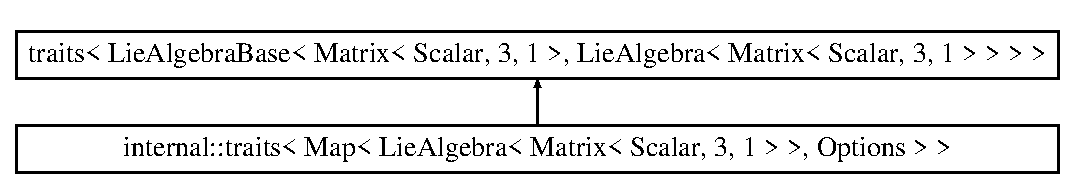
\includegraphics[height=2.000000cm]{structinternal_1_1traits_3_01_map_3_01_lie_algebra_3_01_matrix_3_01_scalar_00_013_00_011_01_4_01_4_00_01_options_01_4_01_4}
\end{center}
\end{figure}
\subsection*{Public Types}
\begin{DoxyCompactItemize}
\item 
typedef Map$<$ Matrix$<$ Scalar, 3, 1 $>$, Options $>$ \hyperlink{structinternal_1_1traits_3_01_map_3_01_lie_algebra_3_01_matrix_3_01_scalar_00_013_00_011_01_4_01_4_00_01_options_01_4_01_4_a24755baa54832046371ad39bee3aa3f5}{Coefficients}
\item 
typedef \hyperlink{class_lie_group}{Lie\+Group}$<$ Quaternion$<$ Scalar $>$ $>$ \hyperlink{structinternal_1_1traits_3_01_map_3_01_lie_algebra_3_01_matrix_3_01_scalar_00_013_00_011_01_4_01_4_00_01_options_01_4_01_4_a3ade09718f291d48f6471acab1dc0a38}{Group}
\end{DoxyCompactItemize}


\subsection{Detailed Description}
\subsubsection*{template$<$typename Scalar, int Options$>$\newline
struct internal\+::traits$<$ Map$<$ Lie\+Algebra$<$ Matrix$<$ Scalar, 3, 1 $>$ $>$, Options $>$ $>$}



Definition at line 306 of file Lie\+Algebra\+\_\+so3.\+h.



\subsection{Member Typedef Documentation}
\hypertarget{structinternal_1_1traits_3_01_map_3_01_lie_algebra_3_01_matrix_3_01_scalar_00_013_00_011_01_4_01_4_00_01_options_01_4_01_4_a24755baa54832046371ad39bee3aa3f5}{}\label{structinternal_1_1traits_3_01_map_3_01_lie_algebra_3_01_matrix_3_01_scalar_00_013_00_011_01_4_01_4_00_01_options_01_4_01_4_a24755baa54832046371ad39bee3aa3f5} 
\index{internal\+::traits$<$ Map$<$ Lie\+Algebra$<$ Matrix$<$ Scalar, 3, 1 $>$ $>$, Options $>$ $>$@{internal\+::traits$<$ Map$<$ Lie\+Algebra$<$ Matrix$<$ Scalar, 3, 1 $>$ $>$, Options $>$ $>$}!Coefficients@{Coefficients}}
\index{Coefficients@{Coefficients}!internal\+::traits$<$ Map$<$ Lie\+Algebra$<$ Matrix$<$ Scalar, 3, 1 $>$ $>$, Options $>$ $>$@{internal\+::traits$<$ Map$<$ Lie\+Algebra$<$ Matrix$<$ Scalar, 3, 1 $>$ $>$, Options $>$ $>$}}
\subsubsection{\texorpdfstring{Coefficients}{Coefficients}}
{\footnotesize\ttfamily template$<$typename Scalar , int Options$>$ \\
typedef Map$<$Matrix$<$Scalar, 3, 1$>$, Options$>$ internal\+::traits$<$ Map$<$ \hyperlink{class_lie_algebra}{Lie\+Algebra}$<$ Matrix$<$ Scalar, 3, 1 $>$ $>$, Options $>$ $>$\+::\hyperlink{structinternal_1_1traits_3_01_map_3_01_lie_algebra_3_01_matrix_3_01_scalar_00_013_00_011_01_4_01_4_00_01_options_01_4_01_4_a24755baa54832046371ad39bee3aa3f5}{Coefficients}}



Definition at line 309 of file Lie\+Algebra\+\_\+so3.\+h.

\hypertarget{structinternal_1_1traits_3_01_map_3_01_lie_algebra_3_01_matrix_3_01_scalar_00_013_00_011_01_4_01_4_00_01_options_01_4_01_4_a3ade09718f291d48f6471acab1dc0a38}{}\label{structinternal_1_1traits_3_01_map_3_01_lie_algebra_3_01_matrix_3_01_scalar_00_013_00_011_01_4_01_4_00_01_options_01_4_01_4_a3ade09718f291d48f6471acab1dc0a38} 
\index{internal\+::traits$<$ Map$<$ Lie\+Algebra$<$ Matrix$<$ Scalar, 3, 1 $>$ $>$, Options $>$ $>$@{internal\+::traits$<$ Map$<$ Lie\+Algebra$<$ Matrix$<$ Scalar, 3, 1 $>$ $>$, Options $>$ $>$}!Group@{Group}}
\index{Group@{Group}!internal\+::traits$<$ Map$<$ Lie\+Algebra$<$ Matrix$<$ Scalar, 3, 1 $>$ $>$, Options $>$ $>$@{internal\+::traits$<$ Map$<$ Lie\+Algebra$<$ Matrix$<$ Scalar, 3, 1 $>$ $>$, Options $>$ $>$}}
\subsubsection{\texorpdfstring{Group}{Group}}
{\footnotesize\ttfamily template$<$typename Scalar , int Options$>$ \\
typedef \hyperlink{class_lie_group}{Lie\+Group}$<$Quaternion$<$Scalar$>$ $>$ internal\+::traits$<$ Map$<$ \hyperlink{class_lie_algebra}{Lie\+Algebra}$<$ Matrix$<$ Scalar, 3, 1 $>$ $>$, Options $>$ $>$\+::\hyperlink{structinternal_1_1traits_3_01_map_3_01_lie_algebra_3_01_matrix_3_01_scalar_00_013_00_011_01_4_01_4_00_01_options_01_4_01_4_a3ade09718f291d48f6471acab1dc0a38}{Group}}



Definition at line 310 of file Lie\+Algebra\+\_\+so3.\+h.



The documentation for this struct was generated from the following file\+:\begin{DoxyCompactItemize}
\item 
/\+Users/\+Ryan/\+Code/codyco-\/superbuild/libraries/\+Eigen\+Lgsm/unsupported/\+Eigen/src/\+Lgsm/\hyperlink{_lie_algebra__so3_8h}{Lie\+Algebra\+\_\+so3.\+h}\end{DoxyCompactItemize}

\hypertarget{structinternal_1_1traits_3_01_map_3_01_lie_algebra_3_01_matrix_3_01_scalar_00_016_00_011_01_4_01_4_00_01_options_01_4_01_4}{}\section{internal\+:\+:traits$<$ Map$<$ Lie\+Algebra$<$ Matrix$<$ Scalar, 6, 1 $>$ $>$, Options $>$ $>$ Struct Template Reference}
\label{structinternal_1_1traits_3_01_map_3_01_lie_algebra_3_01_matrix_3_01_scalar_00_016_00_011_01_4_01_4_00_01_options_01_4_01_4}\index{internal\+::traits$<$ Map$<$ Lie\+Algebra$<$ Matrix$<$ Scalar, 6, 1 $>$ $>$, Options $>$ $>$@{internal\+::traits$<$ Map$<$ Lie\+Algebra$<$ Matrix$<$ Scalar, 6, 1 $>$ $>$, Options $>$ $>$}}


{\ttfamily \#include $<$Lie\+Algebra\+\_\+se3.\+h$>$}

Inheritance diagram for internal\+:\+:traits$<$ Map$<$ Lie\+Algebra$<$ Matrix$<$ Scalar, 6, 1 $>$ $>$, Options $>$ $>$\+:\begin{figure}[H]
\begin{center}
\leavevmode
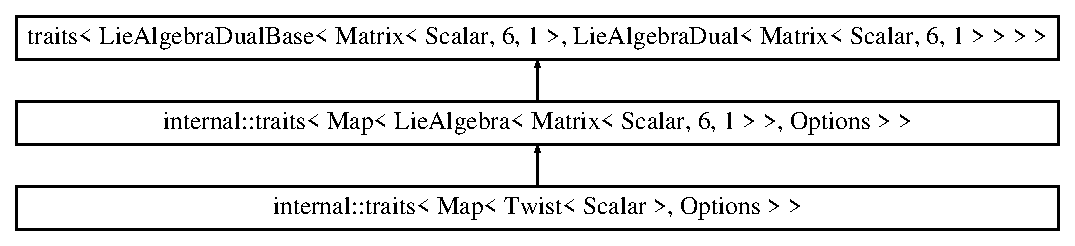
\includegraphics[height=2.857143cm]{structinternal_1_1traits_3_01_map_3_01_lie_algebra_3_01_matrix_3_01_scalar_00_016_00_011_01_4_01_4_00_01_options_01_4_01_4}
\end{center}
\end{figure}
\subsection*{Public Types}
\begin{DoxyCompactItemize}
\item 
typedef Map$<$ Matrix$<$ Scalar, 6, 1 $>$, Options $>$ \hyperlink{structinternal_1_1traits_3_01_map_3_01_lie_algebra_3_01_matrix_3_01_scalar_00_016_00_011_01_4_01_4_00_01_options_01_4_01_4_a3d1c06b436990d5476665a10fc6ec447}{Coefficients}
\item 
typedef \hyperlink{class_lie_group}{Lie\+Group}$<$ Array$<$ Scalar, 7, 1 $>$ $>$ \hyperlink{structinternal_1_1traits_3_01_map_3_01_lie_algebra_3_01_matrix_3_01_scalar_00_016_00_011_01_4_01_4_00_01_options_01_4_01_4_a13ab0b81517271df7b1e26758eb63b67}{Group}
\end{DoxyCompactItemize}


\subsection{Detailed Description}
\subsubsection*{template$<$typename Scalar, int Options$>$\newline
struct internal\+::traits$<$ Map$<$ Lie\+Algebra$<$ Matrix$<$ Scalar, 6, 1 $>$ $>$, Options $>$ $>$}



Definition at line 248 of file Lie\+Algebra\+\_\+se3.\+h.



\subsection{Member Typedef Documentation}
\hypertarget{structinternal_1_1traits_3_01_map_3_01_lie_algebra_3_01_matrix_3_01_scalar_00_016_00_011_01_4_01_4_00_01_options_01_4_01_4_a3d1c06b436990d5476665a10fc6ec447}{}\label{structinternal_1_1traits_3_01_map_3_01_lie_algebra_3_01_matrix_3_01_scalar_00_016_00_011_01_4_01_4_00_01_options_01_4_01_4_a3d1c06b436990d5476665a10fc6ec447} 
\index{internal\+::traits$<$ Map$<$ Lie\+Algebra$<$ Matrix$<$ Scalar, 6, 1 $>$ $>$, Options $>$ $>$@{internal\+::traits$<$ Map$<$ Lie\+Algebra$<$ Matrix$<$ Scalar, 6, 1 $>$ $>$, Options $>$ $>$}!Coefficients@{Coefficients}}
\index{Coefficients@{Coefficients}!internal\+::traits$<$ Map$<$ Lie\+Algebra$<$ Matrix$<$ Scalar, 6, 1 $>$ $>$, Options $>$ $>$@{internal\+::traits$<$ Map$<$ Lie\+Algebra$<$ Matrix$<$ Scalar, 6, 1 $>$ $>$, Options $>$ $>$}}
\subsubsection{\texorpdfstring{Coefficients}{Coefficients}}
{\footnotesize\ttfamily template$<$typename Scalar , int Options$>$ \\
typedef Map$<$Matrix$<$Scalar, 6, 1$>$, Options$>$ internal\+::traits$<$ Map$<$ \hyperlink{class_lie_algebra}{Lie\+Algebra}$<$ Matrix$<$ Scalar, 6, 1 $>$ $>$, Options $>$ $>$\+::\hyperlink{structinternal_1_1traits_3_01_map_3_01_lie_algebra_3_01_matrix_3_01_scalar_00_016_00_011_01_4_01_4_00_01_options_01_4_01_4_a3d1c06b436990d5476665a10fc6ec447}{Coefficients}}



Definition at line 251 of file Lie\+Algebra\+\_\+se3.\+h.

\hypertarget{structinternal_1_1traits_3_01_map_3_01_lie_algebra_3_01_matrix_3_01_scalar_00_016_00_011_01_4_01_4_00_01_options_01_4_01_4_a13ab0b81517271df7b1e26758eb63b67}{}\label{structinternal_1_1traits_3_01_map_3_01_lie_algebra_3_01_matrix_3_01_scalar_00_016_00_011_01_4_01_4_00_01_options_01_4_01_4_a13ab0b81517271df7b1e26758eb63b67} 
\index{internal\+::traits$<$ Map$<$ Lie\+Algebra$<$ Matrix$<$ Scalar, 6, 1 $>$ $>$, Options $>$ $>$@{internal\+::traits$<$ Map$<$ Lie\+Algebra$<$ Matrix$<$ Scalar, 6, 1 $>$ $>$, Options $>$ $>$}!Group@{Group}}
\index{Group@{Group}!internal\+::traits$<$ Map$<$ Lie\+Algebra$<$ Matrix$<$ Scalar, 6, 1 $>$ $>$, Options $>$ $>$@{internal\+::traits$<$ Map$<$ Lie\+Algebra$<$ Matrix$<$ Scalar, 6, 1 $>$ $>$, Options $>$ $>$}}
\subsubsection{\texorpdfstring{Group}{Group}}
{\footnotesize\ttfamily template$<$typename Scalar , int Options$>$ \\
typedef \hyperlink{class_lie_group}{Lie\+Group}$<$Array$<$Scalar, 7, 1$>$ $>$ internal\+::traits$<$ Map$<$ \hyperlink{class_lie_algebra}{Lie\+Algebra}$<$ Matrix$<$ Scalar, 6, 1 $>$ $>$, Options $>$ $>$\+::\hyperlink{structinternal_1_1traits_3_01_map_3_01_lie_algebra_3_01_matrix_3_01_scalar_00_016_00_011_01_4_01_4_00_01_options_01_4_01_4_a13ab0b81517271df7b1e26758eb63b67}{Group}}



Definition at line 252 of file Lie\+Algebra\+\_\+se3.\+h.



The documentation for this struct was generated from the following file\+:\begin{DoxyCompactItemize}
\item 
/\+Users/\+Ryan/\+Code/codyco-\/superbuild/libraries/\+Eigen\+Lgsm/unsupported/\+Eigen/src/\+Lgsm/\hyperlink{_lie_algebra__se3_8h}{Lie\+Algebra\+\_\+se3.\+h}\end{DoxyCompactItemize}

\hypertarget{structinternal_1_1traits_3_01_map_3_01_lie_algebra_dual_3_01_a_01_4_00_01_map_options_00_01_stride_type_01_4_01_4}{}\section{internal\+:\+:traits$<$ Map$<$ Lie\+Algebra\+Dual$<$ A $>$, Map\+Options, Stride\+Type $>$ $>$ Struct Template Reference}
\label{structinternal_1_1traits_3_01_map_3_01_lie_algebra_dual_3_01_a_01_4_00_01_map_options_00_01_stride_type_01_4_01_4}\index{internal\+::traits$<$ Map$<$ Lie\+Algebra\+Dual$<$ A $>$, Map\+Options, Stride\+Type $>$ $>$@{internal\+::traits$<$ Map$<$ Lie\+Algebra\+Dual$<$ A $>$, Map\+Options, Stride\+Type $>$ $>$}}


{\ttfamily \#include $<$Lie\+Algebra.\+h$>$}

Inheritance diagram for internal\+:\+:traits$<$ Map$<$ Lie\+Algebra\+Dual$<$ A $>$, Map\+Options, Stride\+Type $>$ $>$\+:\begin{figure}[H]
\begin{center}
\leavevmode
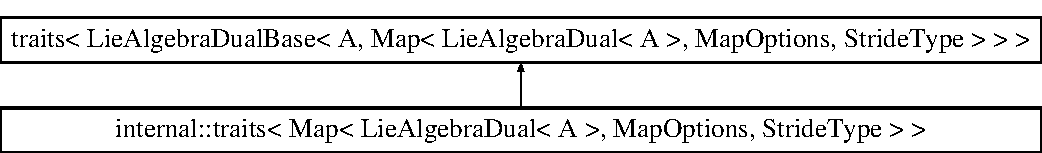
\includegraphics[height=2.000000cm]{structinternal_1_1traits_3_01_map_3_01_lie_algebra_dual_3_01_a_01_4_00_01_map_options_00_01_stride_type_01_4_01_4}
\end{center}
\end{figure}
\subsection*{Public Types}
\begin{DoxyCompactItemize}
\item 
typedef Map$<$ A, Map\+Options, Stride\+Type $>$ \hyperlink{structinternal_1_1traits_3_01_map_3_01_lie_algebra_dual_3_01_a_01_4_00_01_map_options_00_01_stride_type_01_4_01_4_ac32d899dac63614bee761abd9fd3241d}{Coefficients}
\end{DoxyCompactItemize}


\subsection{Detailed Description}
\subsubsection*{template$<$class A, int Map\+Options, typename Stride\+Type$>$\newline
struct internal\+::traits$<$ Map$<$ Lie\+Algebra\+Dual$<$ A $>$, Map\+Options, Stride\+Type $>$ $>$}



Definition at line 343 of file Lie\+Algebra.\+h.



\subsection{Member Typedef Documentation}
\hypertarget{structinternal_1_1traits_3_01_map_3_01_lie_algebra_dual_3_01_a_01_4_00_01_map_options_00_01_stride_type_01_4_01_4_ac32d899dac63614bee761abd9fd3241d}{}\label{structinternal_1_1traits_3_01_map_3_01_lie_algebra_dual_3_01_a_01_4_00_01_map_options_00_01_stride_type_01_4_01_4_ac32d899dac63614bee761abd9fd3241d} 
\index{internal\+::traits$<$ Map$<$ Lie\+Algebra\+Dual$<$ A $>$, Map\+Options, Stride\+Type $>$ $>$@{internal\+::traits$<$ Map$<$ Lie\+Algebra\+Dual$<$ A $>$, Map\+Options, Stride\+Type $>$ $>$}!Coefficients@{Coefficients}}
\index{Coefficients@{Coefficients}!internal\+::traits$<$ Map$<$ Lie\+Algebra\+Dual$<$ A $>$, Map\+Options, Stride\+Type $>$ $>$@{internal\+::traits$<$ Map$<$ Lie\+Algebra\+Dual$<$ A $>$, Map\+Options, Stride\+Type $>$ $>$}}
\subsubsection{\texorpdfstring{Coefficients}{Coefficients}}
{\footnotesize\ttfamily template$<$class A , int Map\+Options, typename Stride\+Type $>$ \\
typedef Map$<$A, Map\+Options, Stride\+Type$>$ internal\+::traits$<$ Map$<$ \hyperlink{class_lie_algebra_dual}{Lie\+Algebra\+Dual}$<$ A $>$, Map\+Options, Stride\+Type $>$ $>$\+::\hyperlink{structinternal_1_1traits_3_01_map_3_01_lie_algebra_dual_3_01_a_01_4_00_01_map_options_00_01_stride_type_01_4_01_4_ac32d899dac63614bee761abd9fd3241d}{Coefficients}}



Definition at line 345 of file Lie\+Algebra.\+h.



The documentation for this struct was generated from the following file\+:\begin{DoxyCompactItemize}
\item 
/\+Users/\+Ryan/\+Code/codyco-\/superbuild/libraries/\+Eigen\+Lgsm/unsupported/\+Eigen/src/\+Lgsm/\hyperlink{_lie_algebra_8h}{Lie\+Algebra.\+h}\end{DoxyCompactItemize}

\hypertarget{structinternal_1_1traits_3_01_map_3_01_lie_algebra_dual_3_01_matrix_3_01_scalar_00_013_00_011_01e8a24fa295b52ac8e6af43d3afd0f30d}{}\section{internal\+:\+:traits$<$ Map$<$ Lie\+Algebra\+Dual$<$ Matrix$<$ Scalar, 3, 1 $>$ $>$, Map\+Options $>$ $>$ Struct Template Reference}
\label{structinternal_1_1traits_3_01_map_3_01_lie_algebra_dual_3_01_matrix_3_01_scalar_00_013_00_011_01e8a24fa295b52ac8e6af43d3afd0f30d}\index{internal\+::traits$<$ Map$<$ Lie\+Algebra\+Dual$<$ Matrix$<$ Scalar, 3, 1 $>$ $>$, Map\+Options $>$ $>$@{internal\+::traits$<$ Map$<$ Lie\+Algebra\+Dual$<$ Matrix$<$ Scalar, 3, 1 $>$ $>$, Map\+Options $>$ $>$}}


{\ttfamily \#include $<$Lie\+Algebra\+\_\+so3.\+h$>$}

Inheritance diagram for internal\+:\+:traits$<$ Map$<$ Lie\+Algebra\+Dual$<$ Matrix$<$ Scalar, 3, 1 $>$ $>$, Map\+Options $>$ $>$\+:\begin{figure}[H]
\begin{center}
\leavevmode
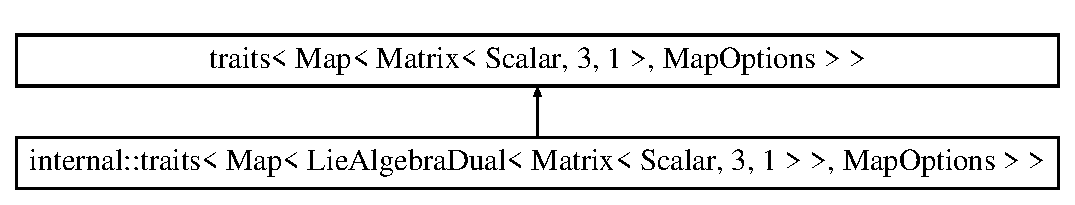
\includegraphics[height=2.000000cm]{structinternal_1_1traits_3_01_map_3_01_lie_algebra_dual_3_01_matrix_3_01_scalar_00_013_00_011_01e8a24fa295b52ac8e6af43d3afd0f30d}
\end{center}
\end{figure}
\subsection*{Public Types}
\begin{DoxyCompactItemize}
\item 
typedef Map$<$ Matrix$<$ Scalar, 3, 1 $>$, Map\+Options $>$ \hyperlink{structinternal_1_1traits_3_01_map_3_01_lie_algebra_dual_3_01_matrix_3_01_scalar_00_013_00_011_01e8a24fa295b52ac8e6af43d3afd0f30d_ab5f11b84b668c4441e8bc5864fd37e84}{Coefficients}
\item 
typedef \hyperlink{class_lie_group}{Lie\+Group}$<$ Quaternion$<$ Scalar $>$ $>$ \hyperlink{structinternal_1_1traits_3_01_map_3_01_lie_algebra_dual_3_01_matrix_3_01_scalar_00_013_00_011_01e8a24fa295b52ac8e6af43d3afd0f30d_a9922d6f6d1e181a21318ebee9de891d2}{Group}
\end{DoxyCompactItemize}


\subsection{Detailed Description}
\subsubsection*{template$<$typename Scalar, int Map\+Options$>$\newline
struct internal\+::traits$<$ Map$<$ Lie\+Algebra\+Dual$<$ Matrix$<$ Scalar, 3, 1 $>$ $>$, Map\+Options $>$ $>$}



Definition at line 265 of file Lie\+Algebra\+\_\+so3.\+h.



\subsection{Member Typedef Documentation}
\hypertarget{structinternal_1_1traits_3_01_map_3_01_lie_algebra_dual_3_01_matrix_3_01_scalar_00_013_00_011_01e8a24fa295b52ac8e6af43d3afd0f30d_ab5f11b84b668c4441e8bc5864fd37e84}{}\label{structinternal_1_1traits_3_01_map_3_01_lie_algebra_dual_3_01_matrix_3_01_scalar_00_013_00_011_01e8a24fa295b52ac8e6af43d3afd0f30d_ab5f11b84b668c4441e8bc5864fd37e84} 
\index{internal\+::traits$<$ Map$<$ Lie\+Algebra\+Dual$<$ Matrix$<$ Scalar, 3, 1 $>$ $>$, Map\+Options $>$ $>$@{internal\+::traits$<$ Map$<$ Lie\+Algebra\+Dual$<$ Matrix$<$ Scalar, 3, 1 $>$ $>$, Map\+Options $>$ $>$}!Coefficients@{Coefficients}}
\index{Coefficients@{Coefficients}!internal\+::traits$<$ Map$<$ Lie\+Algebra\+Dual$<$ Matrix$<$ Scalar, 3, 1 $>$ $>$, Map\+Options $>$ $>$@{internal\+::traits$<$ Map$<$ Lie\+Algebra\+Dual$<$ Matrix$<$ Scalar, 3, 1 $>$ $>$, Map\+Options $>$ $>$}}
\subsubsection{\texorpdfstring{Coefficients}{Coefficients}}
{\footnotesize\ttfamily template$<$typename Scalar , int Map\+Options$>$ \\
typedef Map$<$Matrix$<$Scalar, 3, 1$>$, Map\+Options$>$ internal\+::traits$<$ Map$<$ \hyperlink{class_lie_algebra_dual}{Lie\+Algebra\+Dual}$<$ Matrix$<$ Scalar, 3, 1 $>$ $>$, Map\+Options $>$ $>$\+::\hyperlink{structinternal_1_1traits_3_01_map_3_01_lie_algebra_dual_3_01_matrix_3_01_scalar_00_013_00_011_01e8a24fa295b52ac8e6af43d3afd0f30d_ab5f11b84b668c4441e8bc5864fd37e84}{Coefficients}}



Definition at line 267 of file Lie\+Algebra\+\_\+so3.\+h.

\hypertarget{structinternal_1_1traits_3_01_map_3_01_lie_algebra_dual_3_01_matrix_3_01_scalar_00_013_00_011_01e8a24fa295b52ac8e6af43d3afd0f30d_a9922d6f6d1e181a21318ebee9de891d2}{}\label{structinternal_1_1traits_3_01_map_3_01_lie_algebra_dual_3_01_matrix_3_01_scalar_00_013_00_011_01e8a24fa295b52ac8e6af43d3afd0f30d_a9922d6f6d1e181a21318ebee9de891d2} 
\index{internal\+::traits$<$ Map$<$ Lie\+Algebra\+Dual$<$ Matrix$<$ Scalar, 3, 1 $>$ $>$, Map\+Options $>$ $>$@{internal\+::traits$<$ Map$<$ Lie\+Algebra\+Dual$<$ Matrix$<$ Scalar, 3, 1 $>$ $>$, Map\+Options $>$ $>$}!Group@{Group}}
\index{Group@{Group}!internal\+::traits$<$ Map$<$ Lie\+Algebra\+Dual$<$ Matrix$<$ Scalar, 3, 1 $>$ $>$, Map\+Options $>$ $>$@{internal\+::traits$<$ Map$<$ Lie\+Algebra\+Dual$<$ Matrix$<$ Scalar, 3, 1 $>$ $>$, Map\+Options $>$ $>$}}
\subsubsection{\texorpdfstring{Group}{Group}}
{\footnotesize\ttfamily template$<$typename Scalar , int Map\+Options$>$ \\
typedef \hyperlink{class_lie_group}{Lie\+Group}$<$Quaternion$<$Scalar$>$ $>$ internal\+::traits$<$ Map$<$ \hyperlink{class_lie_algebra_dual}{Lie\+Algebra\+Dual}$<$ Matrix$<$ Scalar, 3, 1 $>$ $>$, Map\+Options $>$ $>$\+::\hyperlink{structinternal_1_1traits_3_01_map_3_01_lie_algebra_dual_3_01_matrix_3_01_scalar_00_013_00_011_01e8a24fa295b52ac8e6af43d3afd0f30d_a9922d6f6d1e181a21318ebee9de891d2}{Group}}



Definition at line 268 of file Lie\+Algebra\+\_\+so3.\+h.



The documentation for this struct was generated from the following file\+:\begin{DoxyCompactItemize}
\item 
/\+Users/\+Ryan/\+Code/codyco-\/superbuild/libraries/\+Eigen\+Lgsm/unsupported/\+Eigen/src/\+Lgsm/\hyperlink{_lie_algebra__so3_8h}{Lie\+Algebra\+\_\+so3.\+h}\end{DoxyCompactItemize}

\hypertarget{structinternal_1_1traits_3_01_map_3_01_lie_group_3_01_g_01_4_00_01_map_options_00_01_stride_type_01_4_01_4}{}\section{internal\+:\+:traits$<$ Map$<$ Lie\+Group$<$ G $>$, Map\+Options, Stride\+Type $>$ $>$ Struct Template Reference}
\label{structinternal_1_1traits_3_01_map_3_01_lie_group_3_01_g_01_4_00_01_map_options_00_01_stride_type_01_4_01_4}\index{internal\+::traits$<$ Map$<$ Lie\+Group$<$ G $>$, Map\+Options, Stride\+Type $>$ $>$@{internal\+::traits$<$ Map$<$ Lie\+Group$<$ G $>$, Map\+Options, Stride\+Type $>$ $>$}}


{\ttfamily \#include $<$Lie\+Group.\+h$>$}

Inheritance diagram for internal\+:\+:traits$<$ Map$<$ Lie\+Group$<$ G $>$, Map\+Options, Stride\+Type $>$ $>$\+:\begin{figure}[H]
\begin{center}
\leavevmode
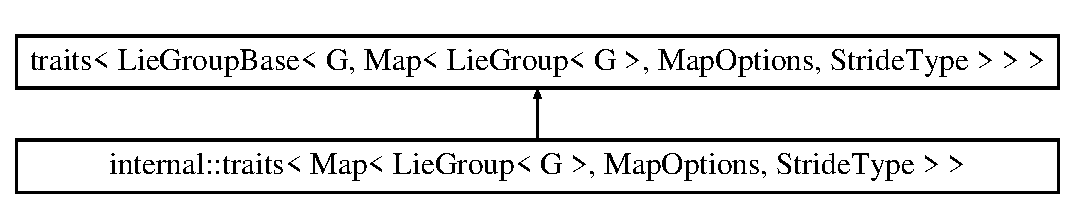
\includegraphics[height=2.000000cm]{structinternal_1_1traits_3_01_map_3_01_lie_group_3_01_g_01_4_00_01_map_options_00_01_stride_type_01_4_01_4}
\end{center}
\end{figure}
\subsection*{Public Types}
\begin{DoxyCompactItemize}
\item 
typedef Map$<$ G, Map\+Options, Stride\+Type $>$ \hyperlink{structinternal_1_1traits_3_01_map_3_01_lie_group_3_01_g_01_4_00_01_map_options_00_01_stride_type_01_4_01_4_ae1223cb79de3b5f754afbacf6b0b956f}{Coefficients}
\item 
typedef G\+::\+Scalar \hyperlink{structinternal_1_1traits_3_01_map_3_01_lie_group_3_01_g_01_4_00_01_map_options_00_01_stride_type_01_4_01_4_ac813c011f308189694ce54531fa28da5}{Scalar}
\end{DoxyCompactItemize}


\subsection{Detailed Description}
\subsubsection*{template$<$class G, int Map\+Options, typename Stride\+Type$>$\newline
struct internal\+::traits$<$ Map$<$ Lie\+Group$<$ G $>$, Map\+Options, Stride\+Type $>$ $>$}



Definition at line 150 of file Lie\+Group.\+h.



\subsection{Member Typedef Documentation}
\hypertarget{structinternal_1_1traits_3_01_map_3_01_lie_group_3_01_g_01_4_00_01_map_options_00_01_stride_type_01_4_01_4_ae1223cb79de3b5f754afbacf6b0b956f}{}\label{structinternal_1_1traits_3_01_map_3_01_lie_group_3_01_g_01_4_00_01_map_options_00_01_stride_type_01_4_01_4_ae1223cb79de3b5f754afbacf6b0b956f} 
\index{internal\+::traits$<$ Map$<$ Lie\+Group$<$ G $>$, Map\+Options, Stride\+Type $>$ $>$@{internal\+::traits$<$ Map$<$ Lie\+Group$<$ G $>$, Map\+Options, Stride\+Type $>$ $>$}!Coefficients@{Coefficients}}
\index{Coefficients@{Coefficients}!internal\+::traits$<$ Map$<$ Lie\+Group$<$ G $>$, Map\+Options, Stride\+Type $>$ $>$@{internal\+::traits$<$ Map$<$ Lie\+Group$<$ G $>$, Map\+Options, Stride\+Type $>$ $>$}}
\subsubsection{\texorpdfstring{Coefficients}{Coefficients}}
{\footnotesize\ttfamily template$<$class G , int Map\+Options, typename Stride\+Type $>$ \\
typedef Map$<$G, Map\+Options, Stride\+Type$>$ internal\+::traits$<$ Map$<$ \hyperlink{class_lie_group}{Lie\+Group}$<$ G $>$, Map\+Options, Stride\+Type $>$ $>$\+::\hyperlink{structinternal_1_1traits_3_01_map_3_01_lie_group_3_01_g_01_4_00_01_map_options_00_01_stride_type_01_4_01_4_ae1223cb79de3b5f754afbacf6b0b956f}{Coefficients}}



Definition at line 152 of file Lie\+Group.\+h.

\hypertarget{structinternal_1_1traits_3_01_map_3_01_lie_group_3_01_g_01_4_00_01_map_options_00_01_stride_type_01_4_01_4_ac813c011f308189694ce54531fa28da5}{}\label{structinternal_1_1traits_3_01_map_3_01_lie_group_3_01_g_01_4_00_01_map_options_00_01_stride_type_01_4_01_4_ac813c011f308189694ce54531fa28da5} 
\index{internal\+::traits$<$ Map$<$ Lie\+Group$<$ G $>$, Map\+Options, Stride\+Type $>$ $>$@{internal\+::traits$<$ Map$<$ Lie\+Group$<$ G $>$, Map\+Options, Stride\+Type $>$ $>$}!Scalar@{Scalar}}
\index{Scalar@{Scalar}!internal\+::traits$<$ Map$<$ Lie\+Group$<$ G $>$, Map\+Options, Stride\+Type $>$ $>$@{internal\+::traits$<$ Map$<$ Lie\+Group$<$ G $>$, Map\+Options, Stride\+Type $>$ $>$}}
\subsubsection{\texorpdfstring{Scalar}{Scalar}}
{\footnotesize\ttfamily template$<$class G , int Map\+Options, typename Stride\+Type $>$ \\
typedef G\+::\+Scalar internal\+::traits$<$ Map$<$ \hyperlink{class_lie_group}{Lie\+Group}$<$ G $>$, Map\+Options, Stride\+Type $>$ $>$\+::\hyperlink{structinternal_1_1traits_3_01_map_3_01_lie_group_3_01_g_01_4_00_01_map_options_00_01_stride_type_01_4_01_4_ac813c011f308189694ce54531fa28da5}{Scalar}}



Definition at line 153 of file Lie\+Group.\+h.



The documentation for this struct was generated from the following file\+:\begin{DoxyCompactItemize}
\item 
/\+Users/\+Ryan/\+Code/codyco-\/superbuild/libraries/\+Eigen\+Lgsm/unsupported/\+Eigen/src/\+Lgsm/\hyperlink{_lie_group_8h}{Lie\+Group.\+h}\end{DoxyCompactItemize}

\hypertarget{structinternal_1_1traits_3_01_map_3_01_twist_3_01_scalar_01_4_00_01_options_01_4_01_4}{}\section{internal\+:\+:traits$<$ Map$<$ Twist$<$ Scalar $>$, Options $>$ $>$ Struct Template Reference}
\label{structinternal_1_1traits_3_01_map_3_01_twist_3_01_scalar_01_4_00_01_options_01_4_01_4}\index{internal\+::traits$<$ Map$<$ Twist$<$ Scalar $>$, Options $>$ $>$@{internal\+::traits$<$ Map$<$ Twist$<$ Scalar $>$, Options $>$ $>$}}


{\ttfamily \#include $<$Twist.\+h$>$}

Inheritance diagram for internal\+:\+:traits$<$ Map$<$ Twist$<$ Scalar $>$, Options $>$ $>$\+:\begin{figure}[H]
\begin{center}
\leavevmode
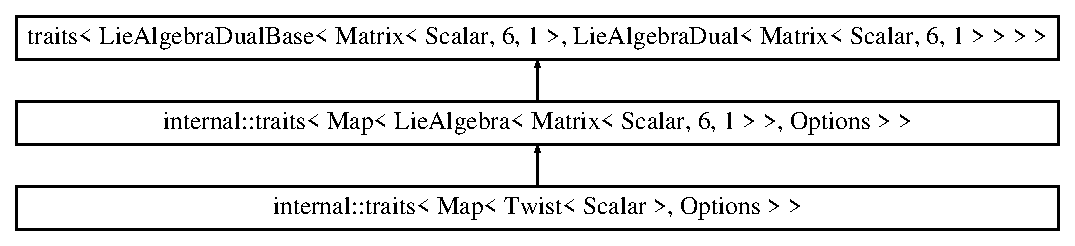
\includegraphics[height=2.857143cm]{structinternal_1_1traits_3_01_map_3_01_twist_3_01_scalar_01_4_00_01_options_01_4_01_4}
\end{center}
\end{figure}
\subsection*{Public Types}
\begin{DoxyCompactItemize}
\item 
typedef \hyperlink{class_displacement}{Displacement}$<$ Scalar $>$ \hyperlink{structinternal_1_1traits_3_01_map_3_01_twist_3_01_scalar_01_4_00_01_options_01_4_01_4_a523550b7b4340ecfa108c8f8126ed636}{Group}
\end{DoxyCompactItemize}


\subsection{Detailed Description}
\subsubsection*{template$<$typename Scalar, int Options$>$\newline
struct internal\+::traits$<$ Map$<$ Twist$<$ Scalar $>$, Options $>$ $>$}



Definition at line 123 of file Twist.\+h.



\subsection{Member Typedef Documentation}
\hypertarget{structinternal_1_1traits_3_01_map_3_01_twist_3_01_scalar_01_4_00_01_options_01_4_01_4_a523550b7b4340ecfa108c8f8126ed636}{}\label{structinternal_1_1traits_3_01_map_3_01_twist_3_01_scalar_01_4_00_01_options_01_4_01_4_a523550b7b4340ecfa108c8f8126ed636} 
\index{internal\+::traits$<$ Map$<$ Twist$<$ Scalar $>$, Options $>$ $>$@{internal\+::traits$<$ Map$<$ Twist$<$ Scalar $>$, Options $>$ $>$}!Group@{Group}}
\index{Group@{Group}!internal\+::traits$<$ Map$<$ Twist$<$ Scalar $>$, Options $>$ $>$@{internal\+::traits$<$ Map$<$ Twist$<$ Scalar $>$, Options $>$ $>$}}
\subsubsection{\texorpdfstring{Group}{Group}}
{\footnotesize\ttfamily template$<$typename Scalar , int Options$>$ \\
typedef \hyperlink{class_displacement}{Displacement}$<$Scalar$>$ internal\+::traits$<$ Map$<$ \hyperlink{class_twist}{Twist}$<$ Scalar $>$, Options $>$ $>$\+::\hyperlink{structinternal_1_1traits_3_01_map_3_01_lie_algebra_3_01_matrix_3_01_scalar_00_016_00_011_01_4_01_4_00_01_options_01_4_01_4_a13ab0b81517271df7b1e26758eb63b67}{Group}}



Definition at line 126 of file Twist.\+h.



The documentation for this struct was generated from the following file\+:\begin{DoxyCompactItemize}
\item 
/\+Users/\+Ryan/\+Code/codyco-\/superbuild/libraries/\+Eigen\+Lgsm/unsupported/\+Eigen/src/\+Lgsm/\hyperlink{_twist_8h}{Twist.\+h}\end{DoxyCompactItemize}

\hypertarget{structinternal_1_1traits_3_01_map_3_01_wrench_3_01___scalar_01_4_00_01_map_options_00_01_stride_type_01_4_01_4}{}\section{internal\+:\+:traits$<$ Map$<$ Wrench$<$ \+\_\+\+Scalar $>$, Map\+Options, Stride\+Type $>$ $>$ Struct Template Reference}
\label{structinternal_1_1traits_3_01_map_3_01_wrench_3_01___scalar_01_4_00_01_map_options_00_01_stride_type_01_4_01_4}\index{internal\+::traits$<$ Map$<$ Wrench$<$ \+\_\+\+Scalar $>$, Map\+Options, Stride\+Type $>$ $>$@{internal\+::traits$<$ Map$<$ Wrench$<$ \+\_\+\+Scalar $>$, Map\+Options, Stride\+Type $>$ $>$}}


{\ttfamily \#include $<$Wrench.\+h$>$}

Inheritance diagram for internal\+:\+:traits$<$ Map$<$ Wrench$<$ \+\_\+\+Scalar $>$, Map\+Options, Stride\+Type $>$ $>$\+:\begin{figure}[H]
\begin{center}
\leavevmode
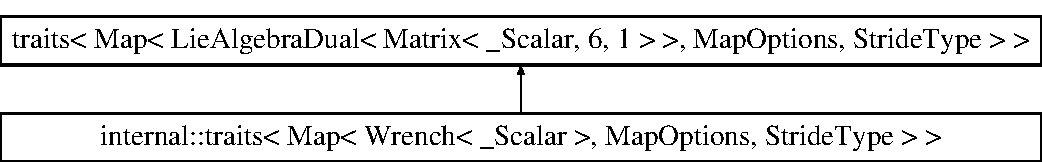
\includegraphics[height=2.000000cm]{structinternal_1_1traits_3_01_map_3_01_wrench_3_01___scalar_01_4_00_01_map_options_00_01_stride_type_01_4_01_4}
\end{center}
\end{figure}
\subsection*{Public Types}
\begin{DoxyCompactItemize}
\item 
typedef \+\_\+\+Scalar \hyperlink{structinternal_1_1traits_3_01_map_3_01_wrench_3_01___scalar_01_4_00_01_map_options_00_01_stride_type_01_4_01_4_a6983b7aa4af5e3133aee4135b962a8a9}{Scalar}
\end{DoxyCompactItemize}


\subsection{Detailed Description}
\subsubsection*{template$<$typename \+\_\+\+Scalar, int Map\+Options, typename Stride\+Type$>$\newline
struct internal\+::traits$<$ Map$<$ Wrench$<$ \+\_\+\+Scalar $>$, Map\+Options, Stride\+Type $>$ $>$}



Definition at line 201 of file Wrench.\+h.



\subsection{Member Typedef Documentation}
\hypertarget{structinternal_1_1traits_3_01_map_3_01_wrench_3_01___scalar_01_4_00_01_map_options_00_01_stride_type_01_4_01_4_a6983b7aa4af5e3133aee4135b962a8a9}{}\label{structinternal_1_1traits_3_01_map_3_01_wrench_3_01___scalar_01_4_00_01_map_options_00_01_stride_type_01_4_01_4_a6983b7aa4af5e3133aee4135b962a8a9} 
\index{internal\+::traits$<$ Map$<$ Wrench$<$ \+\_\+\+Scalar $>$, Map\+Options, Stride\+Type $>$ $>$@{internal\+::traits$<$ Map$<$ Wrench$<$ \+\_\+\+Scalar $>$, Map\+Options, Stride\+Type $>$ $>$}!Scalar@{Scalar}}
\index{Scalar@{Scalar}!internal\+::traits$<$ Map$<$ Wrench$<$ \+\_\+\+Scalar $>$, Map\+Options, Stride\+Type $>$ $>$@{internal\+::traits$<$ Map$<$ Wrench$<$ \+\_\+\+Scalar $>$, Map\+Options, Stride\+Type $>$ $>$}}
\subsubsection{\texorpdfstring{Scalar}{Scalar}}
{\footnotesize\ttfamily template$<$typename \+\_\+\+Scalar , int Map\+Options, typename Stride\+Type $>$ \\
typedef \+\_\+\+Scalar internal\+::traits$<$ Map$<$ \hyperlink{class_wrench}{Wrench}$<$ \+\_\+\+Scalar $>$, Map\+Options, Stride\+Type $>$ $>$\+::\hyperlink{structinternal_1_1traits_3_01_map_3_01_wrench_3_01___scalar_01_4_00_01_map_options_00_01_stride_type_01_4_01_4_a6983b7aa4af5e3133aee4135b962a8a9}{Scalar}}



Definition at line 203 of file Wrench.\+h.



The documentation for this struct was generated from the following file\+:\begin{DoxyCompactItemize}
\item 
/\+Users/\+Ryan/\+Code/codyco-\/superbuild/libraries/\+Eigen\+Lgsm/unsupported/\+Eigen/src/\+Lgsm/\hyperlink{_wrench_8h}{Wrench.\+h}\end{DoxyCompactItemize}

\hypertarget{structinternal_1_1traits_3_01_twist_3_01_scalar_01_4_01_4}{}\section{internal\+:\+:traits$<$ Twist$<$ Scalar $>$ $>$ Struct Template Reference}
\label{structinternal_1_1traits_3_01_twist_3_01_scalar_01_4_01_4}\index{internal\+::traits$<$ Twist$<$ Scalar $>$ $>$@{internal\+::traits$<$ Twist$<$ Scalar $>$ $>$}}


{\ttfamily \#include $<$Twist.\+h$>$}

Inheritance diagram for internal\+:\+:traits$<$ Twist$<$ Scalar $>$ $>$\+:\begin{figure}[H]
\begin{center}
\leavevmode
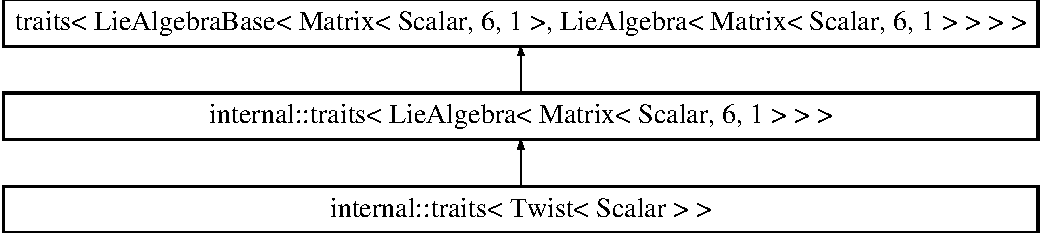
\includegraphics[height=3.000000cm]{structinternal_1_1traits_3_01_twist_3_01_scalar_01_4_01_4}
\end{center}
\end{figure}
\subsection*{Public Types}
\begin{DoxyCompactItemize}
\item 
typedef \hyperlink{class_displacement}{Displacement}$<$ Scalar $>$ \hyperlink{structinternal_1_1traits_3_01_twist_3_01_scalar_01_4_01_4_a7dd4af76dbf2ef6b4e68ceb1249d14c9}{Group}
\end{DoxyCompactItemize}


\subsection{Detailed Description}
\subsubsection*{template$<$typename Scalar$>$\newline
struct internal\+::traits$<$ Twist$<$ Scalar $>$ $>$}



Definition at line 116 of file Twist.\+h.



\subsection{Member Typedef Documentation}
\hypertarget{structinternal_1_1traits_3_01_twist_3_01_scalar_01_4_01_4_a7dd4af76dbf2ef6b4e68ceb1249d14c9}{}\label{structinternal_1_1traits_3_01_twist_3_01_scalar_01_4_01_4_a7dd4af76dbf2ef6b4e68ceb1249d14c9} 
\index{internal\+::traits$<$ Twist$<$ Scalar $>$ $>$@{internal\+::traits$<$ Twist$<$ Scalar $>$ $>$}!Group@{Group}}
\index{Group@{Group}!internal\+::traits$<$ Twist$<$ Scalar $>$ $>$@{internal\+::traits$<$ Twist$<$ Scalar $>$ $>$}}
\subsubsection{\texorpdfstring{Group}{Group}}
{\footnotesize\ttfamily template$<$typename Scalar $>$ \\
typedef \hyperlink{class_displacement}{Displacement}$<$Scalar$>$ internal\+::traits$<$ \hyperlink{class_twist}{Twist}$<$ Scalar $>$ $>$\+::\hyperlink{structinternal_1_1traits_3_01_lie_algebra_3_01_matrix_3_01_scalar_00_016_00_011_01_4_01_4_01_4_a2a6e55a56a1c0c3b97c50cb8598ac55a}{Group}}



Definition at line 119 of file Twist.\+h.



The documentation for this struct was generated from the following file\+:\begin{DoxyCompactItemize}
\item 
/\+Users/\+Ryan/\+Code/codyco-\/superbuild/libraries/\+Eigen\+Lgsm/unsupported/\+Eigen/src/\+Lgsm/\hyperlink{_twist_8h}{Twist.\+h}\end{DoxyCompactItemize}

\hypertarget{structinternal_1_1traits_3_01_twist_base_3_01_derived_01_4_01_4}{}\section{internal\+:\+:traits$<$ Twist\+Base$<$ Derived $>$ $>$ Struct Template Reference}
\label{structinternal_1_1traits_3_01_twist_base_3_01_derived_01_4_01_4}\index{internal\+::traits$<$ Twist\+Base$<$ Derived $>$ $>$@{internal\+::traits$<$ Twist\+Base$<$ Derived $>$ $>$}}


{\ttfamily \#include $<$Twist.\+h$>$}

Inheritance diagram for internal\+:\+:traits$<$ Twist\+Base$<$ Derived $>$ $>$\+:\begin{figure}[H]
\begin{center}
\leavevmode
\includegraphics[height=2.000000cm]{structinternal_1_1traits_3_01_twist_base_3_01_derived_01_4_01_4}
\end{center}
\end{figure}


\subsection{Detailed Description}
\subsubsection*{template$<$class Derived$>$\newline
struct internal\+::traits$<$ Twist\+Base$<$ Derived $>$ $>$}



Definition at line 30 of file Twist.\+h.



The documentation for this struct was generated from the following file\+:\begin{DoxyCompactItemize}
\item 
/\+Users/\+Ryan/\+Code/codyco-\/superbuild/libraries/\+Eigen\+Lgsm/unsupported/\+Eigen/src/\+Lgsm/\hyperlink{_twist_8h}{Twist.\+h}\end{DoxyCompactItemize}

\hypertarget{structinternal_1_1traits_3_01_wrench_3_01___scalar_01_4_01_4}{}\section{internal\+:\+:traits$<$ Wrench$<$ \+\_\+\+Scalar $>$ $>$ Struct Template Reference}
\label{structinternal_1_1traits_3_01_wrench_3_01___scalar_01_4_01_4}\index{internal\+::traits$<$ Wrench$<$ \+\_\+\+Scalar $>$ $>$@{internal\+::traits$<$ Wrench$<$ \+\_\+\+Scalar $>$ $>$}}


{\ttfamily \#include $<$Wrench.\+h$>$}

Inheritance diagram for internal\+:\+:traits$<$ Wrench$<$ \+\_\+\+Scalar $>$ $>$\+:\begin{figure}[H]
\begin{center}
\leavevmode
\includegraphics[height=2.000000cm]{structinternal_1_1traits_3_01_wrench_3_01___scalar_01_4_01_4}
\end{center}
\end{figure}
\subsection*{Public Types}
\begin{DoxyCompactItemize}
\item 
typedef \+\_\+\+Scalar \hyperlink{structinternal_1_1traits_3_01_wrench_3_01___scalar_01_4_01_4_ad1e23cc3d2be914db89e28e5c26b87e1}{Scalar}
\end{DoxyCompactItemize}


\subsection{Detailed Description}
\subsubsection*{template$<$typename \+\_\+\+Scalar$>$\newline
struct internal\+::traits$<$ Wrench$<$ \+\_\+\+Scalar $>$ $>$}



Definition at line 118 of file Wrench.\+h.



\subsection{Member Typedef Documentation}
\hypertarget{structinternal_1_1traits_3_01_wrench_3_01___scalar_01_4_01_4_ad1e23cc3d2be914db89e28e5c26b87e1}{}\label{structinternal_1_1traits_3_01_wrench_3_01___scalar_01_4_01_4_ad1e23cc3d2be914db89e28e5c26b87e1} 
\index{internal\+::traits$<$ Wrench$<$ \+\_\+\+Scalar $>$ $>$@{internal\+::traits$<$ Wrench$<$ \+\_\+\+Scalar $>$ $>$}!Scalar@{Scalar}}
\index{Scalar@{Scalar}!internal\+::traits$<$ Wrench$<$ \+\_\+\+Scalar $>$ $>$@{internal\+::traits$<$ Wrench$<$ \+\_\+\+Scalar $>$ $>$}}
\subsubsection{\texorpdfstring{Scalar}{Scalar}}
{\footnotesize\ttfamily template$<$typename \+\_\+\+Scalar $>$ \\
typedef \+\_\+\+Scalar internal\+::traits$<$ \hyperlink{class_wrench}{Wrench}$<$ \+\_\+\+Scalar $>$ $>$\+::\hyperlink{structinternal_1_1traits_3_01_wrench_3_01___scalar_01_4_01_4_ad1e23cc3d2be914db89e28e5c26b87e1}{Scalar}}



Definition at line 120 of file Wrench.\+h.



The documentation for this struct was generated from the following file\+:\begin{DoxyCompactItemize}
\item 
/\+Users/\+Ryan/\+Code/codyco-\/superbuild/libraries/\+Eigen\+Lgsm/unsupported/\+Eigen/src/\+Lgsm/\hyperlink{_wrench_8h}{Wrench.\+h}\end{DoxyCompactItemize}

\hypertarget{structinternal_1_1traits_3_01_wrench_base_3_01_derived_01_4_01_4}{}\section{internal\+:\+:traits$<$ Wrench\+Base$<$ Derived $>$ $>$ Struct Template Reference}
\label{structinternal_1_1traits_3_01_wrench_base_3_01_derived_01_4_01_4}\index{internal\+::traits$<$ Wrench\+Base$<$ Derived $>$ $>$@{internal\+::traits$<$ Wrench\+Base$<$ Derived $>$ $>$}}


{\ttfamily \#include $<$Wrench.\+h$>$}

Inheritance diagram for internal\+:\+:traits$<$ Wrench\+Base$<$ Derived $>$ $>$\+:\begin{figure}[H]
\begin{center}
\leavevmode
\includegraphics[height=2.000000cm]{structinternal_1_1traits_3_01_wrench_base_3_01_derived_01_4_01_4}
\end{center}
\end{figure}


\subsection{Detailed Description}
\subsubsection*{template$<$class Derived$>$\newline
struct internal\+::traits$<$ Wrench\+Base$<$ Derived $>$ $>$}



Definition at line 30 of file Wrench.\+h.



The documentation for this struct was generated from the following file\+:\begin{DoxyCompactItemize}
\item 
/\+Users/\+Ryan/\+Code/codyco-\/superbuild/libraries/\+Eigen\+Lgsm/unsupported/\+Eigen/src/\+Lgsm/\hyperlink{_wrench_8h}{Wrench.\+h}\end{DoxyCompactItemize}

\hypertarget{class_twist}{}\section{Twist$<$ \+\_\+\+Scalar $>$ Class Template Reference}
\label{class_twist}\index{Twist$<$ \+\_\+\+Scalar $>$@{Twist$<$ \+\_\+\+Scalar $>$}}


Class describing a \hyperlink{class_twist}{Twist}.  




{\ttfamily \#include $<$Twist.\+h$>$}

Inheritance diagram for Twist$<$ \+\_\+\+Scalar $>$\+:\begin{figure}[H]
\begin{center}
\leavevmode
\includegraphics[height=3.943662cm]{class_twist}
\end{center}
\end{figure}
\subsection*{Public Types}
\begin{DoxyCompactItemize}
\item 
typedef \hyperlink{class_twist_base_a4086aa35326778872a7d0f0bfdfcc0ec}{Base\+::\+Base\+Type} \hyperlink{class_twist_ab1df1af2243738177191f6c23123f3be}{Base\+Type}
\item 
typedef internal\+::traits$<$ \hyperlink{class_twist}{Twist} $>$\+::\hyperlink{class_twist_a1bc0976a0f06b366421639350134222b}{Coefficients} \hyperlink{class_twist_a1bc0976a0f06b366421639350134222b}{Coefficients}
\end{DoxyCompactItemize}
\subsection*{Public Member Functions}
\begin{DoxyCompactItemize}
\item 
\hyperlink{class_twist_a1591bb5cbaf556a1315950e4b27a50cf}{Twist} ()
\item 
\hyperlink{class_twist_a6d27b4287aff94955d46b3f76151f119}{Twist} (const \hyperlink{class_twist}{Twist} \&g)
\item 
\hyperlink{class_twist_a4b460b4e069b959f7fd2f0d01fdf4703}{Twist} (const \hyperlink{class_twist_ab1df1af2243738177191f6c23123f3be}{Base\+Type} \&g)
\item 
\hyperlink{class_twist_adf2846cc99f0b092b4ab622a00177363}{Twist} (Scalar \hyperlink{class_twist_base_a894919d086a24def57622d7e151a58c2}{rx}, Scalar \hyperlink{class_twist_base_a649f10b163fa68cd901aa3ee412ced7f}{ry}, Scalar \hyperlink{class_twist_base_a25f415854bcf537c8aa1cc244bfdb770}{rz}, Scalar \hyperlink{class_twist_base_a323021f263783da2d5b275552858ab67}{vx}, Scalar \hyperlink{class_twist_base_a2cf70ed359f60d07610e8ab36910f436}{vy}, Scalar \hyperlink{class_twist_base_a217ab4d995e5c40b24a586278301415e}{vz})
\item 
{\footnotesize template$<$typename Other\+Derived $>$ }\\E\+I\+G\+E\+N\+\_\+\+S\+T\+R\+O\+N\+G\+\_\+\+I\+N\+L\+I\+NE \hyperlink{class_twist_ace92bbcbb4ccc4da3bf3f98c2463aca6}{Twist} (const Matrix\+Base$<$ Other\+Derived $>$ \&other)
\item 
{\footnotesize template$<$class Linear\+Velocity\+Derived , class Angular\+Velocity\+Derived $>$ }\\\hyperlink{class_twist_ac948ffd308a2af9bb8fbd68cda5e1331}{Twist} (const \hyperlink{class_lie_algebra_base}{Lie\+Algebra\+Base}$<$ Matrix$<$ Scalar, 3, 1 $>$, Angular\+Velocity\+Derived $>$ \&r, const Matrix\+Base$<$ Linear\+Velocity\+Derived $>$ \&v)
\item 
\hyperlink{class_twist_a6be65e5ed24f7aa0b2ac0261aa111292}{Twist} (const typename \hyperlink{class_twist_base_ad0bc13debe8afc170da877cebe4dc45f}{Base\+::\+Angular\+Velocity} \&r, const typename \hyperlink{class_twist_base_aeafbc7a3ca37e08812be0af7e680190b}{Base\+::\+Linear\+Velocity} \&v)
\item 
\hyperlink{class_twist_a1bc0976a0f06b366421639350134222b}{Coefficients} \& \hyperlink{class_twist_ac1f779976c880605099c319bc9749c2c}{get} ()
\item 
const \hyperlink{class_twist_a1bc0976a0f06b366421639350134222b}{Coefficients} \& \hyperlink{class_twist_a92329266374466e60daabe5ca6c2dcbe}{get} () const
\end{DoxyCompactItemize}
\subsection*{Protected Types}
\begin{DoxyCompactItemize}
\item 
typedef \hyperlink{class_twist_base}{Twist\+Base}$<$ \hyperlink{class_twist}{Twist}$<$ \+\_\+\+Scalar $>$ $>$ \hyperlink{class_twist_a83c55648035a111abdce59e32880a710}{Base}
\end{DoxyCompactItemize}
\subsection*{Protected Attributes}
\begin{DoxyCompactItemize}
\item 
\hyperlink{class_twist_a1bc0976a0f06b366421639350134222b}{Coefficients} \hyperlink{class_twist_ac4b3ab83b5a42bc592b55dbb94905c4e}{m\+\_\+coeffs}
\end{DoxyCompactItemize}


\subsection{Detailed Description}
\subsubsection*{template$<$typename \+\_\+\+Scalar$>$\newline
class Twist$<$ \+\_\+\+Scalar $>$}

Class describing a \hyperlink{class_twist}{Twist}. 


\begin{DoxyTemplParams}{Template Parameters}
{\em \+\_\+\+Scalar} & the type of the underlying array\\
\hline
\end{DoxyTemplParams}
This class add some specific constructors

\begin{DoxySeeAlso}{See also}
The methods are defined in \hyperlink{class_lie_algebra_base}{Lie\+Algebra\+Base} and \hyperlink{class_twist_base}{Twist\+Base} 
\end{DoxySeeAlso}


Definition at line 141 of file Twist.\+h.



\subsection{Member Typedef Documentation}
\hypertarget{class_twist_a83c55648035a111abdce59e32880a710}{}\label{class_twist_a83c55648035a111abdce59e32880a710} 
\index{Twist@{Twist}!Base@{Base}}
\index{Base@{Base}!Twist@{Twist}}
\subsubsection{\texorpdfstring{Base}{Base}}
{\footnotesize\ttfamily template$<$typename \+\_\+\+Scalar$>$ \\
typedef \hyperlink{class_twist_base}{Twist\+Base}$<$\hyperlink{class_twist}{Twist}$<$\+\_\+\+Scalar$>$ $>$ \hyperlink{class_twist}{Twist}$<$ \+\_\+\+Scalar $>$\+::\hyperlink{class_twist_a83c55648035a111abdce59e32880a710}{Base}\hspace{0.3cm}{\ttfamily [protected]}}



Definition at line 143 of file Twist.\+h.

\hypertarget{class_twist_ab1df1af2243738177191f6c23123f3be}{}\label{class_twist_ab1df1af2243738177191f6c23123f3be} 
\index{Twist@{Twist}!Base\+Type@{Base\+Type}}
\index{Base\+Type@{Base\+Type}!Twist@{Twist}}
\subsubsection{\texorpdfstring{Base\+Type}{BaseType}}
{\footnotesize\ttfamily template$<$typename \+\_\+\+Scalar$>$ \\
typedef \hyperlink{class_twist_base_a4086aa35326778872a7d0f0bfdfcc0ec}{Base\+::\+Base\+Type} \hyperlink{class_twist}{Twist}$<$ \+\_\+\+Scalar $>$\+::\hyperlink{class_twist_ab1df1af2243738177191f6c23123f3be}{Base\+Type}}

The inherited class 

Definition at line 151 of file Twist.\+h.

\hypertarget{class_twist_a1bc0976a0f06b366421639350134222b}{}\label{class_twist_a1bc0976a0f06b366421639350134222b} 
\index{Twist@{Twist}!Coefficients@{Coefficients}}
\index{Coefficients@{Coefficients}!Twist@{Twist}}
\subsubsection{\texorpdfstring{Coefficients}{Coefficients}}
{\footnotesize\ttfamily template$<$typename \+\_\+\+Scalar$>$ \\
typedef internal\+::traits$<$\hyperlink{class_twist}{Twist}$>$\+::\hyperlink{class_twist_a1bc0976a0f06b366421639350134222b}{Coefficients} \hyperlink{class_twist}{Twist}$<$ \+\_\+\+Scalar $>$\+::\hyperlink{class_twist_a1bc0976a0f06b366421639350134222b}{Coefficients}}

the stored coefficients 

Definition at line 153 of file Twist.\+h.



\subsection{Constructor \& Destructor Documentation}
\hypertarget{class_twist_a1591bb5cbaf556a1315950e4b27a50cf}{}\label{class_twist_a1591bb5cbaf556a1315950e4b27a50cf} 
\index{Twist@{Twist}!Twist@{Twist}}
\index{Twist@{Twist}!Twist@{Twist}}
\subsubsection{\texorpdfstring{Twist()}{Twist()}\hspace{0.1cm}{\footnotesize\ttfamily [1/7]}}
{\footnotesize\ttfamily template$<$typename \+\_\+\+Scalar$>$ \\
\hyperlink{class_twist}{Twist}$<$ \+\_\+\+Scalar $>$\+::\hyperlink{class_twist}{Twist} (\begin{DoxyParamCaption}{ }\end{DoxyParamCaption})\hspace{0.3cm}{\ttfamily [inline]}}

Default constructor 

Definition at line 157 of file Twist.\+h.

\hypertarget{class_twist_a6d27b4287aff94955d46b3f76151f119}{}\label{class_twist_a6d27b4287aff94955d46b3f76151f119} 
\index{Twist@{Twist}!Twist@{Twist}}
\index{Twist@{Twist}!Twist@{Twist}}
\subsubsection{\texorpdfstring{Twist()}{Twist()}\hspace{0.1cm}{\footnotesize\ttfamily [2/7]}}
{\footnotesize\ttfamily template$<$typename \+\_\+\+Scalar$>$ \\
\hyperlink{class_twist}{Twist}$<$ \+\_\+\+Scalar $>$\+::\hyperlink{class_twist}{Twist} (\begin{DoxyParamCaption}\item[{const \hyperlink{class_twist}{Twist}$<$ \+\_\+\+Scalar $>$ \&}]{g }\end{DoxyParamCaption})\hspace{0.3cm}{\ttfamily [inline]}}

Copy constructor 

Definition at line 159 of file Twist.\+h.

\hypertarget{class_twist_a4b460b4e069b959f7fd2f0d01fdf4703}{}\label{class_twist_a4b460b4e069b959f7fd2f0d01fdf4703} 
\index{Twist@{Twist}!Twist@{Twist}}
\index{Twist@{Twist}!Twist@{Twist}}
\subsubsection{\texorpdfstring{Twist()}{Twist()}\hspace{0.1cm}{\footnotesize\ttfamily [3/7]}}
{\footnotesize\ttfamily template$<$typename \+\_\+\+Scalar$>$ \\
\hyperlink{class_twist}{Twist}$<$ \+\_\+\+Scalar $>$\+::\hyperlink{class_twist}{Twist} (\begin{DoxyParamCaption}\item[{const \hyperlink{class_twist_ab1df1af2243738177191f6c23123f3be}{Base\+Type} \&}]{g }\end{DoxyParamCaption})\hspace{0.3cm}{\ttfamily [inline]}}

Copy constructor 

Definition at line 161 of file Twist.\+h.

\hypertarget{class_twist_adf2846cc99f0b092b4ab622a00177363}{}\label{class_twist_adf2846cc99f0b092b4ab622a00177363} 
\index{Twist@{Twist}!Twist@{Twist}}
\index{Twist@{Twist}!Twist@{Twist}}
\subsubsection{\texorpdfstring{Twist()}{Twist()}\hspace{0.1cm}{\footnotesize\ttfamily [4/7]}}
{\footnotesize\ttfamily template$<$typename \+\_\+\+Scalar$>$ \\
\hyperlink{class_twist}{Twist}$<$ \+\_\+\+Scalar $>$\+::\hyperlink{class_twist}{Twist} (\begin{DoxyParamCaption}\item[{Scalar}]{rx,  }\item[{Scalar}]{ry,  }\item[{Scalar}]{rz,  }\item[{Scalar}]{vx,  }\item[{Scalar}]{vy,  }\item[{Scalar}]{vz }\end{DoxyParamCaption})\hspace{0.3cm}{\ttfamily [inline]}}

Constructs an element of se(3) from 6 scalar 

Definition at line 163 of file Twist.\+h.

\hypertarget{class_twist_ace92bbcbb4ccc4da3bf3f98c2463aca6}{}\label{class_twist_ace92bbcbb4ccc4da3bf3f98c2463aca6} 
\index{Twist@{Twist}!Twist@{Twist}}
\index{Twist@{Twist}!Twist@{Twist}}
\subsubsection{\texorpdfstring{Twist()}{Twist()}\hspace{0.1cm}{\footnotesize\ttfamily [5/7]}}
{\footnotesize\ttfamily template$<$typename \+\_\+\+Scalar$>$ \\
template$<$typename Other\+Derived $>$ \\
E\+I\+G\+E\+N\+\_\+\+S\+T\+R\+O\+N\+G\+\_\+\+I\+N\+L\+I\+NE \hyperlink{class_twist}{Twist}$<$ \+\_\+\+Scalar $>$\+::\hyperlink{class_twist}{Twist} (\begin{DoxyParamCaption}\item[{const Matrix\+Base$<$ Other\+Derived $>$ \&}]{other }\end{DoxyParamCaption})\hspace{0.3cm}{\ttfamily [inline]}}

Copy constructor \+: need to build a twist from a C\+Wise\+Binary\+Op or C\+Wise\+Unary\+Op 

Definition at line 173 of file Twist.\+h.

\hypertarget{class_twist_ac948ffd308a2af9bb8fbd68cda5e1331}{}\label{class_twist_ac948ffd308a2af9bb8fbd68cda5e1331} 
\index{Twist@{Twist}!Twist@{Twist}}
\index{Twist@{Twist}!Twist@{Twist}}
\subsubsection{\texorpdfstring{Twist()}{Twist()}\hspace{0.1cm}{\footnotesize\ttfamily [6/7]}}
{\footnotesize\ttfamily template$<$typename \+\_\+\+Scalar$>$ \\
template$<$class Linear\+Velocity\+Derived , class Angular\+Velocity\+Derived $>$ \\
\hyperlink{class_twist}{Twist}$<$ \+\_\+\+Scalar $>$\+::\hyperlink{class_twist}{Twist} (\begin{DoxyParamCaption}\item[{const \hyperlink{class_lie_algebra_base}{Lie\+Algebra\+Base}$<$ Matrix$<$ Scalar, 3, 1 $>$, Angular\+Velocity\+Derived $>$ \&}]{r,  }\item[{const Matrix\+Base$<$ Linear\+Velocity\+Derived $>$ \&}]{v }\end{DoxyParamCaption})\hspace{0.3cm}{\ttfamily [inline]}}

Assignement operator \+: need to copy a C\+Wise\+Binary\+Op or C\+Wise\+Unary\+Op to a \hyperlink{class_twist}{Twist} Constructs \hyperlink{class_twist}{Twist} from an angular velocity {\ttfamily r} and a linear velocity {\ttfamily v} 

Definition at line 186 of file Twist.\+h.

\hypertarget{class_twist_a6be65e5ed24f7aa0b2ac0261aa111292}{}\label{class_twist_a6be65e5ed24f7aa0b2ac0261aa111292} 
\index{Twist@{Twist}!Twist@{Twist}}
\index{Twist@{Twist}!Twist@{Twist}}
\subsubsection{\texorpdfstring{Twist()}{Twist()}\hspace{0.1cm}{\footnotesize\ttfamily [7/7]}}
{\footnotesize\ttfamily template$<$typename \+\_\+\+Scalar$>$ \\
\hyperlink{class_twist}{Twist}$<$ \+\_\+\+Scalar $>$\+::\hyperlink{class_twist}{Twist} (\begin{DoxyParamCaption}\item[{const typename \hyperlink{class_twist_base_ad0bc13debe8afc170da877cebe4dc45f}{Base\+::\+Angular\+Velocity} \&}]{r,  }\item[{const typename \hyperlink{class_twist_base_aeafbc7a3ca37e08812be0af7e680190b}{Base\+::\+Linear\+Velocity} \&}]{v }\end{DoxyParamCaption})\hspace{0.3cm}{\ttfamily [inline]}}

Constructs \hyperlink{class_twist}{Twist} from an angular velocity {\ttfamily r} and a linear velocity {\ttfamily v} 

Definition at line 191 of file Twist.\+h.



\subsection{Member Function Documentation}
\hypertarget{class_twist_ac1f779976c880605099c319bc9749c2c}{}\label{class_twist_ac1f779976c880605099c319bc9749c2c} 
\index{Twist@{Twist}!get@{get}}
\index{get@{get}!Twist@{Twist}}
\subsubsection{\texorpdfstring{get()}{get()}\hspace{0.1cm}{\footnotesize\ttfamily [1/2]}}
{\footnotesize\ttfamily template$<$typename \+\_\+\+Scalar$>$ \\
\hyperlink{class_twist_a1bc0976a0f06b366421639350134222b}{Coefficients}\& \hyperlink{class_twist}{Twist}$<$ \+\_\+\+Scalar $>$\+::get (\begin{DoxyParamCaption}{ }\end{DoxyParamCaption})\hspace{0.3cm}{\ttfamily [inline]}}

\begin{DoxyReturn}{Returns}
The stored coefficients 
\end{DoxyReturn}


Definition at line 196 of file Twist.\+h.

\hypertarget{class_twist_a92329266374466e60daabe5ca6c2dcbe}{}\label{class_twist_a92329266374466e60daabe5ca6c2dcbe} 
\index{Twist@{Twist}!get@{get}}
\index{get@{get}!Twist@{Twist}}
\subsubsection{\texorpdfstring{get()}{get()}\hspace{0.1cm}{\footnotesize\ttfamily [2/2]}}
{\footnotesize\ttfamily template$<$typename \+\_\+\+Scalar$>$ \\
const \hyperlink{class_twist_a1bc0976a0f06b366421639350134222b}{Coefficients}\& \hyperlink{class_twist}{Twist}$<$ \+\_\+\+Scalar $>$\+::get (\begin{DoxyParamCaption}{ }\end{DoxyParamCaption}) const\hspace{0.3cm}{\ttfamily [inline]}}

\begin{DoxyReturn}{Returns}
The read-\/only access to the stored coefficients 
\end{DoxyReturn}


Definition at line 198 of file Twist.\+h.



\subsection{Member Data Documentation}
\hypertarget{class_twist_ac4b3ab83b5a42bc592b55dbb94905c4e}{}\label{class_twist_ac4b3ab83b5a42bc592b55dbb94905c4e} 
\index{Twist@{Twist}!m\+\_\+coeffs@{m\+\_\+coeffs}}
\index{m\+\_\+coeffs@{m\+\_\+coeffs}!Twist@{Twist}}
\subsubsection{\texorpdfstring{m\+\_\+coeffs}{m\_coeffs}}
{\footnotesize\ttfamily template$<$typename \+\_\+\+Scalar$>$ \\
\hyperlink{class_twist_a1bc0976a0f06b366421639350134222b}{Coefficients} \hyperlink{class_twist}{Twist}$<$ \+\_\+\+Scalar $>$\+::m\+\_\+coeffs\hspace{0.3cm}{\ttfamily [protected]}}

The wrapped coefficients 

Definition at line 202 of file Twist.\+h.



The documentation for this class was generated from the following file\+:\begin{DoxyCompactItemize}
\item 
/\+Users/\+Ryan/\+Code/codyco-\/superbuild/libraries/\+Eigen\+Lgsm/unsupported/\+Eigen/src/\+Lgsm/\hyperlink{_twist_8h}{Twist.\+h}\end{DoxyCompactItemize}

\hypertarget{class_twist_base}{}\section{Twist\+Base$<$ Derived $>$ Class Template Reference}
\label{class_twist_base}\index{Twist\+Base$<$ Derived $>$@{Twist\+Base$<$ Derived $>$}}


Base class describing a \hyperlink{class_twist}{Twist}.  




{\ttfamily \#include $<$Twist.\+h$>$}

Inheritance diagram for Twist\+Base$<$ Derived $>$\+:\begin{figure}[H]
\begin{center}
\leavevmode
\includegraphics[height=3.000000cm]{class_twist_base}
\end{center}
\end{figure}
\subsection*{Public Types}
\begin{DoxyCompactItemize}
\item 
typedef \hyperlink{class_lie_algebra_base_3_01_matrix_3_01typename_01internal_1_1traits_3_01_derived_01_4_1_1_scala449314c781550590437697c4dc21a6d4_abb811fe29a9ece0ee6f2239f17fea23f}{Base\+::\+Base\+Type} \hyperlink{class_twist_base_a4086aa35326778872a7d0f0bfdfcc0ec}{Base\+Type}
\item 
typedef internal\+::traits$<$ Derived $>$\+::\hyperlink{class_twist_base_a773de67da6fe03840b5178517b17e75c}{Coefficients} \hyperlink{class_twist_base_a773de67da6fe03840b5178517b17e75c}{Coefficients}
\item 
typedef Matrix$<$ Scalar, 3, 1 $>$ \hyperlink{class_twist_base_aeafbc7a3ca37e08812be0af7e680190b}{Linear\+Velocity}
\item 
typedef \hyperlink{class_lie_algebra}{Lie\+Algebra}$<$ Matrix$<$ Scalar, 3, 1 $>$ $>$ \hyperlink{class_twist_base_ad0bc13debe8afc170da877cebe4dc45f}{Angular\+Velocity}
\end{DoxyCompactItemize}
\subsection*{Public Member Functions}
\begin{DoxyCompactItemize}
\item 
Scalar \hyperlink{class_twist_base_a894919d086a24def57622d7e151a58c2}{rx} () const
\item 
Scalar \hyperlink{class_twist_base_a649f10b163fa68cd901aa3ee412ced7f}{ry} () const
\item 
Scalar \hyperlink{class_twist_base_a25f415854bcf537c8aa1cc244bfdb770}{rz} () const
\item 
Scalar \hyperlink{class_twist_base_a323021f263783da2d5b275552858ab67}{vx} () const
\item 
Scalar \hyperlink{class_twist_base_a2cf70ed359f60d07610e8ab36910f436}{vy} () const
\item 
Scalar \hyperlink{class_twist_base_a217ab4d995e5c40b24a586278301415e}{vz} () const
\item 
Scalar \& \hyperlink{class_twist_base_a9622270eb8e0f450bce5b356ee10f205}{rx} ()
\item 
Scalar \& \hyperlink{class_twist_base_a43c3b5462cb4f4b71283e29871b89cd1}{ry} ()
\item 
Scalar \& \hyperlink{class_twist_base_a0ca49c0005a9a87ddebd2e3892687529}{rz} ()
\item 
Scalar \& \hyperlink{class_twist_base_a8d4de5b2cf8cfdeab7146777cbeec798}{vx} ()
\item 
Scalar \& \hyperlink{class_twist_base_aea73eb77920e10bfdbc01cc1fd7956f8}{vy} ()
\item 
Scalar \& \hyperlink{class_twist_base_a169c415ee48933c6820131d211b38eac}{vz} ()
\item 
Map$<$ \hyperlink{class_twist_base_ad0bc13debe8afc170da877cebe4dc45f}{Angular\+Velocity} $>$ \hyperlink{class_twist_base_a9574d52bbded5a52ee8ae7d69f462c1b}{get\+Angular\+Velocity} ()
\item 
Map$<$ const \hyperlink{class_twist_base_ad0bc13debe8afc170da877cebe4dc45f}{Angular\+Velocity} $>$ \hyperlink{class_twist_base_ab6e1055a88a9d729290272d62b7bb128}{get\+Angular\+Velocity} () const
\item 
Map$<$ \hyperlink{class_twist_base_aeafbc7a3ca37e08812be0af7e680190b}{Linear\+Velocity} $>$ \hyperlink{class_twist_base_a8056931a50cd7fa4f0d75f70470b0907}{get\+Linear\+Velocity} ()
\item 
Map$<$ const \hyperlink{class_twist_base_aeafbc7a3ca37e08812be0af7e680190b}{Linear\+Velocity} $>$ \hyperlink{class_twist_base_ae0ea0ad07e9f5547cd18a8f6eb953792}{get\+Linear\+Velocity} () const
\item 
{\footnotesize template$<$class Rotation\+Derived $>$ }\\\hyperlink{class_twist}{Twist}$<$ Scalar $>$ \hyperlink{class_twist_base_a6c88583539f3cd30d68576ea4d707525}{change\+Frame} (const \hyperlink{class_lie_group_base}{Lie\+Group\+Base}$<$ Quaternion$<$ Scalar $>$, Rotation\+Derived $>$ \&) const
\item 
{\footnotesize template$<$class Other\+Derived $>$ }\\\hyperlink{class_twist}{Twist}$<$ Scalar $>$ \hyperlink{class_twist_base_a44ecd77777c54f0f632d6a89951c5884}{change\+Point} (const Matrix\+Base$<$ Other\+Derived $>$ \&point) const
\item 
{\footnotesize template$<$class Rotation\+Derived $>$ }\\\hyperlink{class_twist}{Twist}$<$ typename internal\+::traits$<$ \hyperlink{class_twist_base}{Twist\+Base}$<$ Derived $>$ $>$\+::Scalar $>$ \hyperlink{class_twist_base_a6e0074ec6e0621dc603d6eca78b4d9f2}{change\+Frame} (const \hyperlink{class_lie_group_base}{Lie\+Group\+Base}$<$ Quaternion$<$ Scalar $>$, Rotation\+Derived $>$ \&rot) const
\item 
{\footnotesize template$<$class Other\+Derived $>$ }\\\hyperlink{class_twist}{Twist}$<$ typename internal\+::traits$<$ \hyperlink{class_twist_base}{Twist\+Base}$<$ Derived $>$ $>$\+::Scalar $>$ \hyperlink{class_twist_base_a9cc4e024b42a1164268d8066b006289c}{change\+Point} (const Matrix\+Base$<$ Other\+Derived $>$ \&point) const
\end{DoxyCompactItemize}
\subsection*{Protected Types}
\begin{DoxyCompactItemize}
\item 
typedef \hyperlink{class_lie_algebra_base}{Lie\+Algebra\+Base}$<$ Matrix$<$ typename internal\+::traits$<$ Derived $>$\+::Scalar, 6, 1 $>$, Derived $>$ \hyperlink{class_twist_base_a5855f503803bbb643e270d0cc7360c1f}{Base}
\end{DoxyCompactItemize}


\subsection{Detailed Description}
\subsubsection*{template$<$class Derived$>$\newline
class Twist\+Base$<$ Derived $>$}

Base class describing a \hyperlink{class_twist}{Twist}. 


\begin{DoxyTemplParams}{Template Parameters}
{\em Derived} & the derived class holding the coefficients which are of type Matrix$<$\+Scalar, 6, 1$>$ or Map$<$Matrix$<$\+Scalar, 6, 1$>$ $>$\\
\hline
\end{DoxyTemplParams}
This class abstracts the underlying mathematical definition and add some accessors. A twist has two part, an angular velocity and a linear velocity. It uses an Matrix internally to store its coefficients. 

Definition at line 35 of file Twist.\+h.



\subsection{Member Typedef Documentation}
\hypertarget{class_twist_base_ad0bc13debe8afc170da877cebe4dc45f}{}\label{class_twist_base_ad0bc13debe8afc170da877cebe4dc45f} 
\index{Twist\+Base@{Twist\+Base}!Angular\+Velocity@{Angular\+Velocity}}
\index{Angular\+Velocity@{Angular\+Velocity}!Twist\+Base@{Twist\+Base}}
\subsubsection{\texorpdfstring{Angular\+Velocity}{AngularVelocity}}
{\footnotesize\ttfamily template$<$class Derived$>$ \\
typedef \hyperlink{class_lie_algebra}{Lie\+Algebra}$<$Matrix$<$Scalar, 3, 1$>$ $>$ \hyperlink{class_twist_base}{Twist\+Base}$<$ Derived $>$\+::\hyperlink{class_twist_base_ad0bc13debe8afc170da877cebe4dc45f}{Angular\+Velocity}}

The type of the angular part 

Definition at line 79 of file Twist.\+h.

\hypertarget{class_twist_base_a5855f503803bbb643e270d0cc7360c1f}{}\label{class_twist_base_a5855f503803bbb643e270d0cc7360c1f} 
\index{Twist\+Base@{Twist\+Base}!Base@{Base}}
\index{Base@{Base}!Twist\+Base@{Twist\+Base}}
\subsubsection{\texorpdfstring{Base}{Base}}
{\footnotesize\ttfamily template$<$class Derived$>$ \\
typedef \hyperlink{class_lie_algebra_base}{Lie\+Algebra\+Base}$<$Matrix$<$typename internal\+::traits$<$Derived$>$\+::Scalar, 6, 1$>$, Derived$>$ \hyperlink{class_twist_base}{Twist\+Base}$<$ Derived $>$\+::\hyperlink{class_twist_base_a5855f503803bbb643e270d0cc7360c1f}{Base}\hspace{0.3cm}{\ttfamily [protected]}}

The inherited class 

Definition at line 38 of file Twist.\+h.

\hypertarget{class_twist_base_a4086aa35326778872a7d0f0bfdfcc0ec}{}\label{class_twist_base_a4086aa35326778872a7d0f0bfdfcc0ec} 
\index{Twist\+Base@{Twist\+Base}!Base\+Type@{Base\+Type}}
\index{Base\+Type@{Base\+Type}!Twist\+Base@{Twist\+Base}}
\subsubsection{\texorpdfstring{Base\+Type}{BaseType}}
{\footnotesize\ttfamily template$<$class Derived$>$ \\
typedef \hyperlink{class_lie_algebra_base_3_01_matrix_3_01typename_01internal_1_1traits_3_01_derived_01_4_1_1_scala449314c781550590437697c4dc21a6d4_abb811fe29a9ece0ee6f2239f17fea23f}{Base\+::\+Base\+Type} \hyperlink{class_twist_base}{Twist\+Base}$<$ Derived $>$\+::\hyperlink{class_twist_base_a4086aa35326778872a7d0f0bfdfcc0ec}{Base\+Type}}

The wrapped class 

Definition at line 46 of file Twist.\+h.

\hypertarget{class_twist_base_a773de67da6fe03840b5178517b17e75c}{}\label{class_twist_base_a773de67da6fe03840b5178517b17e75c} 
\index{Twist\+Base@{Twist\+Base}!Coefficients@{Coefficients}}
\index{Coefficients@{Coefficients}!Twist\+Base@{Twist\+Base}}
\subsubsection{\texorpdfstring{Coefficients}{Coefficients}}
{\footnotesize\ttfamily template$<$class Derived$>$ \\
typedef internal\+::traits$<$Derived$>$\+::\hyperlink{class_twist_base_a773de67da6fe03840b5178517b17e75c}{Coefficients} \hyperlink{class_twist_base}{Twist\+Base}$<$ Derived $>$\+::\hyperlink{class_twist_base_a773de67da6fe03840b5178517b17e75c}{Coefficients}}

The kind of stored coefficients 

Definition at line 48 of file Twist.\+h.

\hypertarget{class_twist_base_aeafbc7a3ca37e08812be0af7e680190b}{}\label{class_twist_base_aeafbc7a3ca37e08812be0af7e680190b} 
\index{Twist\+Base@{Twist\+Base}!Linear\+Velocity@{Linear\+Velocity}}
\index{Linear\+Velocity@{Linear\+Velocity}!Twist\+Base@{Twist\+Base}}
\subsubsection{\texorpdfstring{Linear\+Velocity}{LinearVelocity}}
{\footnotesize\ttfamily template$<$class Derived$>$ \\
typedef Matrix$<$Scalar, 3, 1$>$ \hyperlink{class_twist_base}{Twist\+Base}$<$ Derived $>$\+::\hyperlink{class_twist_base_aeafbc7a3ca37e08812be0af7e680190b}{Linear\+Velocity}}

The type of the linear part 

Definition at line 77 of file Twist.\+h.



\subsection{Member Function Documentation}
\hypertarget{class_twist_base_a6c88583539f3cd30d68576ea4d707525}{}\label{class_twist_base_a6c88583539f3cd30d68576ea4d707525} 
\index{Twist\+Base@{Twist\+Base}!change\+Frame@{change\+Frame}}
\index{change\+Frame@{change\+Frame}!Twist\+Base@{Twist\+Base}}
\subsubsection{\texorpdfstring{change\+Frame()}{changeFrame()}\hspace{0.1cm}{\footnotesize\ttfamily [1/2]}}
{\footnotesize\ttfamily template$<$class Derived$>$ \\
template$<$class Rotation\+Derived $>$ \\
\hyperlink{class_twist}{Twist}$<$Scalar$>$ \hyperlink{class_twist_base}{Twist\+Base}$<$ Derived $>$\+::change\+Frame (\begin{DoxyParamCaption}\item[{const \hyperlink{class_lie_group_base}{Lie\+Group\+Base}$<$ Quaternion$<$ Scalar $>$, Rotation\+Derived $>$ \&}]{ }\end{DoxyParamCaption}) const\hspace{0.3cm}{\ttfamily [inline]}}

\hypertarget{class_twist_base_a6e0074ec6e0621dc603d6eca78b4d9f2}{}\label{class_twist_base_a6e0074ec6e0621dc603d6eca78b4d9f2} 
\index{Twist\+Base@{Twist\+Base}!change\+Frame@{change\+Frame}}
\index{change\+Frame@{change\+Frame}!Twist\+Base@{Twist\+Base}}
\subsubsection{\texorpdfstring{change\+Frame()}{changeFrame()}\hspace{0.1cm}{\footnotesize\ttfamily [2/2]}}
{\footnotesize\ttfamily template$<$class Derived$>$ \\
template$<$class Rotation\+Derived $>$ \\
\hyperlink{class_twist}{Twist}$<$typename internal\+::traits$<$\hyperlink{class_twist_base}{Twist\+Base}$<$Derived$>$ $>$\+::Scalar$>$ \hyperlink{class_twist_base}{Twist\+Base}$<$ Derived $>$\+::change\+Frame (\begin{DoxyParamCaption}\item[{const \hyperlink{class_lie_group_base}{Lie\+Group\+Base}$<$ Quaternion$<$ Scalar $>$, Rotation\+Derived $>$ \&}]{rot }\end{DoxyParamCaption}) const\hspace{0.3cm}{\ttfamily [inline]}}



Definition at line 98 of file Twist.\+h.

\hypertarget{class_twist_base_a44ecd77777c54f0f632d6a89951c5884}{}\label{class_twist_base_a44ecd77777c54f0f632d6a89951c5884} 
\index{Twist\+Base@{Twist\+Base}!change\+Point@{change\+Point}}
\index{change\+Point@{change\+Point}!Twist\+Base@{Twist\+Base}}
\subsubsection{\texorpdfstring{change\+Point()}{changePoint()}\hspace{0.1cm}{\footnotesize\ttfamily [1/2]}}
{\footnotesize\ttfamily template$<$class Derived$>$ \\
template$<$class Other\+Derived $>$ \\
\hyperlink{class_twist}{Twist}$<$Scalar$>$ \hyperlink{class_twist_base}{Twist\+Base}$<$ Derived $>$\+::change\+Point (\begin{DoxyParamCaption}\item[{const Matrix\+Base$<$ Other\+Derived $>$ \&}]{point }\end{DoxyParamCaption}) const\hspace{0.3cm}{\ttfamily [inline]}}

\hypertarget{class_twist_base_a9cc4e024b42a1164268d8066b006289c}{}\label{class_twist_base_a9cc4e024b42a1164268d8066b006289c} 
\index{Twist\+Base@{Twist\+Base}!change\+Point@{change\+Point}}
\index{change\+Point@{change\+Point}!Twist\+Base@{Twist\+Base}}
\subsubsection{\texorpdfstring{change\+Point()}{changePoint()}\hspace{0.1cm}{\footnotesize\ttfamily [2/2]}}
{\footnotesize\ttfamily template$<$class Derived$>$ \\
template$<$class Other\+Derived $>$ \\
\hyperlink{class_twist}{Twist}$<$typename internal\+::traits$<$\hyperlink{class_twist_base}{Twist\+Base}$<$Derived$>$ $>$\+::Scalar$>$ \hyperlink{class_twist_base}{Twist\+Base}$<$ Derived $>$\+::change\+Point (\begin{DoxyParamCaption}\item[{const Matrix\+Base$<$ Other\+Derived $>$ \&}]{point }\end{DoxyParamCaption}) const\hspace{0.3cm}{\ttfamily [inline]}}



Definition at line 105 of file Twist.\+h.

\hypertarget{class_twist_base_a9574d52bbded5a52ee8ae7d69f462c1b}{}\label{class_twist_base_a9574d52bbded5a52ee8ae7d69f462c1b} 
\index{Twist\+Base@{Twist\+Base}!get\+Angular\+Velocity@{get\+Angular\+Velocity}}
\index{get\+Angular\+Velocity@{get\+Angular\+Velocity}!Twist\+Base@{Twist\+Base}}
\subsubsection{\texorpdfstring{get\+Angular\+Velocity()}{getAngularVelocity()}\hspace{0.1cm}{\footnotesize\ttfamily [1/2]}}
{\footnotesize\ttfamily template$<$class Derived$>$ \\
Map$<$\hyperlink{class_twist_base_ad0bc13debe8afc170da877cebe4dc45f}{Angular\+Velocity}$>$ \hyperlink{class_twist_base}{Twist\+Base}$<$ Derived $>$\+::get\+Angular\+Velocity (\begin{DoxyParamCaption}{ }\end{DoxyParamCaption})\hspace{0.3cm}{\ttfamily [inline]}}

The accessor to the angular velocity 

Definition at line 82 of file Twist.\+h.

\hypertarget{class_twist_base_ab6e1055a88a9d729290272d62b7bb128}{}\label{class_twist_base_ab6e1055a88a9d729290272d62b7bb128} 
\index{Twist\+Base@{Twist\+Base}!get\+Angular\+Velocity@{get\+Angular\+Velocity}}
\index{get\+Angular\+Velocity@{get\+Angular\+Velocity}!Twist\+Base@{Twist\+Base}}
\subsubsection{\texorpdfstring{get\+Angular\+Velocity()}{getAngularVelocity()}\hspace{0.1cm}{\footnotesize\ttfamily [2/2]}}
{\footnotesize\ttfamily template$<$class Derived$>$ \\
Map$<$const \hyperlink{class_twist_base_ad0bc13debe8afc170da877cebe4dc45f}{Angular\+Velocity}$>$ \hyperlink{class_twist_base}{Twist\+Base}$<$ Derived $>$\+::get\+Angular\+Velocity (\begin{DoxyParamCaption}{ }\end{DoxyParamCaption}) const\hspace{0.3cm}{\ttfamily [inline]}}

The read-\/only accessor to the angular velocity 

Definition at line 84 of file Twist.\+h.

\hypertarget{class_twist_base_a8056931a50cd7fa4f0d75f70470b0907}{}\label{class_twist_base_a8056931a50cd7fa4f0d75f70470b0907} 
\index{Twist\+Base@{Twist\+Base}!get\+Linear\+Velocity@{get\+Linear\+Velocity}}
\index{get\+Linear\+Velocity@{get\+Linear\+Velocity}!Twist\+Base@{Twist\+Base}}
\subsubsection{\texorpdfstring{get\+Linear\+Velocity()}{getLinearVelocity()}\hspace{0.1cm}{\footnotesize\ttfamily [1/2]}}
{\footnotesize\ttfamily template$<$class Derived$>$ \\
Map$<$\hyperlink{class_twist_base_aeafbc7a3ca37e08812be0af7e680190b}{Linear\+Velocity}$>$ \hyperlink{class_twist_base}{Twist\+Base}$<$ Derived $>$\+::get\+Linear\+Velocity (\begin{DoxyParamCaption}{ }\end{DoxyParamCaption})\hspace{0.3cm}{\ttfamily [inline]}}

The accessor to the linear velocity 

Definition at line 86 of file Twist.\+h.

\hypertarget{class_twist_base_ae0ea0ad07e9f5547cd18a8f6eb953792}{}\label{class_twist_base_ae0ea0ad07e9f5547cd18a8f6eb953792} 
\index{Twist\+Base@{Twist\+Base}!get\+Linear\+Velocity@{get\+Linear\+Velocity}}
\index{get\+Linear\+Velocity@{get\+Linear\+Velocity}!Twist\+Base@{Twist\+Base}}
\subsubsection{\texorpdfstring{get\+Linear\+Velocity()}{getLinearVelocity()}\hspace{0.1cm}{\footnotesize\ttfamily [2/2]}}
{\footnotesize\ttfamily template$<$class Derived$>$ \\
Map$<$const \hyperlink{class_twist_base_aeafbc7a3ca37e08812be0af7e680190b}{Linear\+Velocity}$>$ \hyperlink{class_twist_base}{Twist\+Base}$<$ Derived $>$\+::get\+Linear\+Velocity (\begin{DoxyParamCaption}{ }\end{DoxyParamCaption}) const\hspace{0.3cm}{\ttfamily [inline]}}

The read-\/only accessor to the angular velocity 

Definition at line 88 of file Twist.\+h.

\hypertarget{class_twist_base_a894919d086a24def57622d7e151a58c2}{}\label{class_twist_base_a894919d086a24def57622d7e151a58c2} 
\index{Twist\+Base@{Twist\+Base}!rx@{rx}}
\index{rx@{rx}!Twist\+Base@{Twist\+Base}}
\subsubsection{\texorpdfstring{rx()}{rx()}\hspace{0.1cm}{\footnotesize\ttfamily [1/2]}}
{\footnotesize\ttfamily template$<$class Derived$>$ \\
Scalar \hyperlink{class_twist_base}{Twist\+Base}$<$ Derived $>$\+::rx (\begin{DoxyParamCaption}{ }\end{DoxyParamCaption}) const\hspace{0.3cm}{\ttfamily [inline]}}

\begin{DoxyReturn}{Returns}
the {\ttfamily rx} coefficient 
\end{DoxyReturn}


Definition at line 51 of file Twist.\+h.

\hypertarget{class_twist_base_a9622270eb8e0f450bce5b356ee10f205}{}\label{class_twist_base_a9622270eb8e0f450bce5b356ee10f205} 
\index{Twist\+Base@{Twist\+Base}!rx@{rx}}
\index{rx@{rx}!Twist\+Base@{Twist\+Base}}
\subsubsection{\texorpdfstring{rx()}{rx()}\hspace{0.1cm}{\footnotesize\ttfamily [2/2]}}
{\footnotesize\ttfamily template$<$class Derived$>$ \\
Scalar\& \hyperlink{class_twist_base}{Twist\+Base}$<$ Derived $>$\+::rx (\begin{DoxyParamCaption}{ }\end{DoxyParamCaption})\hspace{0.3cm}{\ttfamily [inline]}}

\begin{DoxyReturn}{Returns}
a reference to the {\ttfamily rx} coefficient 
\end{DoxyReturn}


Definition at line 64 of file Twist.\+h.

\hypertarget{class_twist_base_a649f10b163fa68cd901aa3ee412ced7f}{}\label{class_twist_base_a649f10b163fa68cd901aa3ee412ced7f} 
\index{Twist\+Base@{Twist\+Base}!ry@{ry}}
\index{ry@{ry}!Twist\+Base@{Twist\+Base}}
\subsubsection{\texorpdfstring{ry()}{ry()}\hspace{0.1cm}{\footnotesize\ttfamily [1/2]}}
{\footnotesize\ttfamily template$<$class Derived$>$ \\
Scalar \hyperlink{class_twist_base}{Twist\+Base}$<$ Derived $>$\+::ry (\begin{DoxyParamCaption}{ }\end{DoxyParamCaption}) const\hspace{0.3cm}{\ttfamily [inline]}}

\begin{DoxyReturn}{Returns}
the {\ttfamily ry} coefficient 
\end{DoxyReturn}


Definition at line 53 of file Twist.\+h.

\hypertarget{class_twist_base_a43c3b5462cb4f4b71283e29871b89cd1}{}\label{class_twist_base_a43c3b5462cb4f4b71283e29871b89cd1} 
\index{Twist\+Base@{Twist\+Base}!ry@{ry}}
\index{ry@{ry}!Twist\+Base@{Twist\+Base}}
\subsubsection{\texorpdfstring{ry()}{ry()}\hspace{0.1cm}{\footnotesize\ttfamily [2/2]}}
{\footnotesize\ttfamily template$<$class Derived$>$ \\
Scalar\& \hyperlink{class_twist_base}{Twist\+Base}$<$ Derived $>$\+::ry (\begin{DoxyParamCaption}{ }\end{DoxyParamCaption})\hspace{0.3cm}{\ttfamily [inline]}}

\begin{DoxyReturn}{Returns}
a reference to the {\ttfamily ry} coefficient 
\end{DoxyReturn}


Definition at line 66 of file Twist.\+h.

\hypertarget{class_twist_base_a25f415854bcf537c8aa1cc244bfdb770}{}\label{class_twist_base_a25f415854bcf537c8aa1cc244bfdb770} 
\index{Twist\+Base@{Twist\+Base}!rz@{rz}}
\index{rz@{rz}!Twist\+Base@{Twist\+Base}}
\subsubsection{\texorpdfstring{rz()}{rz()}\hspace{0.1cm}{\footnotesize\ttfamily [1/2]}}
{\footnotesize\ttfamily template$<$class Derived$>$ \\
Scalar \hyperlink{class_twist_base}{Twist\+Base}$<$ Derived $>$\+::rz (\begin{DoxyParamCaption}{ }\end{DoxyParamCaption}) const\hspace{0.3cm}{\ttfamily [inline]}}

\begin{DoxyReturn}{Returns}
the {\ttfamily rz} coefficient 
\end{DoxyReturn}


Definition at line 55 of file Twist.\+h.

\hypertarget{class_twist_base_a0ca49c0005a9a87ddebd2e3892687529}{}\label{class_twist_base_a0ca49c0005a9a87ddebd2e3892687529} 
\index{Twist\+Base@{Twist\+Base}!rz@{rz}}
\index{rz@{rz}!Twist\+Base@{Twist\+Base}}
\subsubsection{\texorpdfstring{rz()}{rz()}\hspace{0.1cm}{\footnotesize\ttfamily [2/2]}}
{\footnotesize\ttfamily template$<$class Derived$>$ \\
Scalar\& \hyperlink{class_twist_base}{Twist\+Base}$<$ Derived $>$\+::rz (\begin{DoxyParamCaption}{ }\end{DoxyParamCaption})\hspace{0.3cm}{\ttfamily [inline]}}

\begin{DoxyReturn}{Returns}
a reference to the {\ttfamily rz} coefficient 
\end{DoxyReturn}


Definition at line 68 of file Twist.\+h.

\hypertarget{class_twist_base_a323021f263783da2d5b275552858ab67}{}\label{class_twist_base_a323021f263783da2d5b275552858ab67} 
\index{Twist\+Base@{Twist\+Base}!vx@{vx}}
\index{vx@{vx}!Twist\+Base@{Twist\+Base}}
\subsubsection{\texorpdfstring{vx()}{vx()}\hspace{0.1cm}{\footnotesize\ttfamily [1/2]}}
{\footnotesize\ttfamily template$<$class Derived$>$ \\
Scalar \hyperlink{class_twist_base}{Twist\+Base}$<$ Derived $>$\+::vx (\begin{DoxyParamCaption}{ }\end{DoxyParamCaption}) const\hspace{0.3cm}{\ttfamily [inline]}}

\begin{DoxyReturn}{Returns}
the {\ttfamily vx} coefficient 
\end{DoxyReturn}


Definition at line 57 of file Twist.\+h.

\hypertarget{class_twist_base_a8d4de5b2cf8cfdeab7146777cbeec798}{}\label{class_twist_base_a8d4de5b2cf8cfdeab7146777cbeec798} 
\index{Twist\+Base@{Twist\+Base}!vx@{vx}}
\index{vx@{vx}!Twist\+Base@{Twist\+Base}}
\subsubsection{\texorpdfstring{vx()}{vx()}\hspace{0.1cm}{\footnotesize\ttfamily [2/2]}}
{\footnotesize\ttfamily template$<$class Derived$>$ \\
Scalar\& \hyperlink{class_twist_base}{Twist\+Base}$<$ Derived $>$\+::vx (\begin{DoxyParamCaption}{ }\end{DoxyParamCaption})\hspace{0.3cm}{\ttfamily [inline]}}

\begin{DoxyReturn}{Returns}
a reference to the {\ttfamily vx} coefficient 
\end{DoxyReturn}


Definition at line 70 of file Twist.\+h.

\hypertarget{class_twist_base_a2cf70ed359f60d07610e8ab36910f436}{}\label{class_twist_base_a2cf70ed359f60d07610e8ab36910f436} 
\index{Twist\+Base@{Twist\+Base}!vy@{vy}}
\index{vy@{vy}!Twist\+Base@{Twist\+Base}}
\subsubsection{\texorpdfstring{vy()}{vy()}\hspace{0.1cm}{\footnotesize\ttfamily [1/2]}}
{\footnotesize\ttfamily template$<$class Derived$>$ \\
Scalar \hyperlink{class_twist_base}{Twist\+Base}$<$ Derived $>$\+::vy (\begin{DoxyParamCaption}{ }\end{DoxyParamCaption}) const\hspace{0.3cm}{\ttfamily [inline]}}

\begin{DoxyReturn}{Returns}
the {\ttfamily vy} coefficient 
\end{DoxyReturn}


Definition at line 59 of file Twist.\+h.

\hypertarget{class_twist_base_aea73eb77920e10bfdbc01cc1fd7956f8}{}\label{class_twist_base_aea73eb77920e10bfdbc01cc1fd7956f8} 
\index{Twist\+Base@{Twist\+Base}!vy@{vy}}
\index{vy@{vy}!Twist\+Base@{Twist\+Base}}
\subsubsection{\texorpdfstring{vy()}{vy()}\hspace{0.1cm}{\footnotesize\ttfamily [2/2]}}
{\footnotesize\ttfamily template$<$class Derived$>$ \\
Scalar\& \hyperlink{class_twist_base}{Twist\+Base}$<$ Derived $>$\+::vy (\begin{DoxyParamCaption}{ }\end{DoxyParamCaption})\hspace{0.3cm}{\ttfamily [inline]}}

\begin{DoxyReturn}{Returns}
a reference to the {\ttfamily vy} coefficient 
\end{DoxyReturn}


Definition at line 72 of file Twist.\+h.

\hypertarget{class_twist_base_a217ab4d995e5c40b24a586278301415e}{}\label{class_twist_base_a217ab4d995e5c40b24a586278301415e} 
\index{Twist\+Base@{Twist\+Base}!vz@{vz}}
\index{vz@{vz}!Twist\+Base@{Twist\+Base}}
\subsubsection{\texorpdfstring{vz()}{vz()}\hspace{0.1cm}{\footnotesize\ttfamily [1/2]}}
{\footnotesize\ttfamily template$<$class Derived$>$ \\
Scalar \hyperlink{class_twist_base}{Twist\+Base}$<$ Derived $>$\+::vz (\begin{DoxyParamCaption}{ }\end{DoxyParamCaption}) const\hspace{0.3cm}{\ttfamily [inline]}}

\begin{DoxyReturn}{Returns}
the {\ttfamily vz} coefficient 
\end{DoxyReturn}


Definition at line 61 of file Twist.\+h.

\hypertarget{class_twist_base_a169c415ee48933c6820131d211b38eac}{}\label{class_twist_base_a169c415ee48933c6820131d211b38eac} 
\index{Twist\+Base@{Twist\+Base}!vz@{vz}}
\index{vz@{vz}!Twist\+Base@{Twist\+Base}}
\subsubsection{\texorpdfstring{vz()}{vz()}\hspace{0.1cm}{\footnotesize\ttfamily [2/2]}}
{\footnotesize\ttfamily template$<$class Derived$>$ \\
Scalar\& \hyperlink{class_twist_base}{Twist\+Base}$<$ Derived $>$\+::vz (\begin{DoxyParamCaption}{ }\end{DoxyParamCaption})\hspace{0.3cm}{\ttfamily [inline]}}

\begin{DoxyReturn}{Returns}
a reference to the {\ttfamily vz} coefficient 
\end{DoxyReturn}


Definition at line 74 of file Twist.\+h.



The documentation for this class was generated from the following file\+:\begin{DoxyCompactItemize}
\item 
/\+Users/\+Ryan/\+Code/codyco-\/superbuild/libraries/\+Eigen\+Lgsm/unsupported/\+Eigen/src/\+Lgsm/\hyperlink{_twist_8h}{Twist.\+h}\end{DoxyCompactItemize}

\hypertarget{class_wrench}{}\section{Wrench$<$ \+\_\+\+Scalar $>$ Class Template Reference}
\label{class_wrench}\index{Wrench$<$ \+\_\+\+Scalar $>$@{Wrench$<$ \+\_\+\+Scalar $>$}}


Class describing a \hyperlink{class_wrench}{Wrench}.  




{\ttfamily \#include $<$Wrench.\+h$>$}

Inheritance diagram for Wrench$<$ \+\_\+\+Scalar $>$\+:\begin{figure}[H]
\begin{center}
\leavevmode
\includegraphics[height=3.578275cm]{class_wrench}
\end{center}
\end{figure}
\subsection*{Public Types}
\begin{DoxyCompactItemize}
\item 
typedef \hyperlink{class_wrench_base_a8b98c467c6fb31bd7354dcbef134dca1}{Base\+::\+Base\+Type} \hyperlink{class_wrench_abc5de6653f57de3beb6335e474fc2802}{Base\+Type}
\item 
typedef internal\+::traits$<$ \hyperlink{class_wrench}{Wrench} $>$\+::\hyperlink{class_wrench_a3b7401ec055bd386fc3dc826308784e8}{Coefficients} \hyperlink{class_wrench_a3b7401ec055bd386fc3dc826308784e8}{Coefficients}
\end{DoxyCompactItemize}
\subsection*{Public Member Functions}
\begin{DoxyCompactItemize}
\item 
\hyperlink{class_wrench_a748f2f5a35ee560efa9baa6b7cf3457b}{Wrench} ()
\item 
\hyperlink{class_wrench_a248ef8976ae4ba0cb0023888777be19b}{Wrench} (const \hyperlink{class_wrench}{Wrench} \&g)
\item 
\hyperlink{class_wrench_a39e8751dfbcc808085e7ae9408659243}{Wrench} (const \hyperlink{class_wrench_abc5de6653f57de3beb6335e474fc2802}{Base\+Type} \&g)
\item 
\hyperlink{class_wrench_a9748492aa7f5e07665db15b64a525f9d}{Wrench} (const typename \hyperlink{class_lie_algebra_dual_base_a9b59cead2f78ed837cd22a96155e5da3}{Base\+::\+Plain\+Object} \&g)
\item 
\hyperlink{class_wrench_a82d1e4cba2590bc6380c395012d74102}{Wrench} (Scalar \hyperlink{class_wrench_base_a28eccf6ee6ec9a0e8ad6f0a130c17f0a}{tx}, Scalar \hyperlink{class_wrench_base_a7d574941740c725e035df6af20c0af6c}{ty}, Scalar \hyperlink{class_wrench_base_accf6a99e5dd656d46a0e848add0c9e85}{tz}, Scalar \hyperlink{class_wrench_base_ab4883d6553bab8cbe99737b664cbbd31}{fx}, Scalar \hyperlink{class_wrench_base_a9cf08f34e7d12b9fda2cd521fbca527e}{fy}, Scalar \hyperlink{class_wrench_base_a045d6010d317ce4ee578bfcf1f0162c7}{fz})
\item 
{\footnotesize template$<$typename Other\+Derived $>$ }\\E\+I\+G\+E\+N\+\_\+\+S\+T\+R\+O\+N\+G\+\_\+\+I\+N\+L\+I\+NE \hyperlink{class_wrench_aa3975c26b9d785fc956c86c9bcf82a39}{Wrench} (const Matrix\+Base$<$ Other\+Derived $>$ \&other)
\item 
{\footnotesize template$<$typename Other\+Derived $>$ }\\E\+I\+G\+E\+N\+\_\+\+S\+T\+R\+O\+N\+G\+\_\+\+I\+N\+L\+I\+NE \hyperlink{class_wrench}{Wrench} \& \hyperlink{class_wrench_aaafc24af18da8389e4d7e92c5c4ade90}{operator=} (const Matrix\+Base$<$ Other\+Derived $>$ \&other)
\item 
\hyperlink{class_wrench_a5674ee39466b179af823f10a07427b3a}{Wrench} (const typename \hyperlink{class_wrench_base_a8fa1b5e32e8418247118cc24be70d68d}{Base\+::\+Torque} \&t, const typename \hyperlink{class_wrench_base_aa589699bbf0d18c023a0a2fe6482b4a7}{Base\+::\+Force} \&f)
\item 
\hyperlink{class_wrench_a3b7401ec055bd386fc3dc826308784e8}{Coefficients} \& \hyperlink{class_wrench_abb89a8f4d5642c705ec591f02daaf11a}{get} ()
\item 
const \hyperlink{class_wrench_a3b7401ec055bd386fc3dc826308784e8}{Coefficients} \& \hyperlink{class_wrench_afaea09f03cfc476c06e005d4a338a57f}{get} () const
\end{DoxyCompactItemize}
\subsection*{Protected Types}
\begin{DoxyCompactItemize}
\item 
typedef \hyperlink{class_wrench_base}{Wrench\+Base}$<$ \hyperlink{class_wrench}{Wrench}$<$ \+\_\+\+Scalar $>$ $>$ \hyperlink{class_wrench_a4f3f84e4c6510bc7c0613d9bcb784015}{Base}
\end{DoxyCompactItemize}
\subsection*{Protected Attributes}
\begin{DoxyCompactItemize}
\item 
\hyperlink{class_wrench_a3b7401ec055bd386fc3dc826308784e8}{Coefficients} \hyperlink{class_wrench_a3314bb14c83d52d863490c9460cacbce}{m\+\_\+coeffs}
\end{DoxyCompactItemize}


\subsection{Detailed Description}
\subsubsection*{template$<$typename \+\_\+\+Scalar$>$\newline
class Wrench$<$ \+\_\+\+Scalar $>$}

Class describing a \hyperlink{class_wrench}{Wrench}. 


\begin{DoxyTemplParams}{Template Parameters}
{\em \+\_\+\+Scalar} & the type of the underlying array\\
\hline
\end{DoxyTemplParams}
This class add some specific constructors

\begin{DoxySeeAlso}{See also}
The methods are defined in \hyperlink{class_lie_algebra_base}{Lie\+Algebra\+Base} and \hyperlink{class_wrench_base}{Wrench\+Base} 
\end{DoxySeeAlso}


Definition at line 135 of file Wrench.\+h.



\subsection{Member Typedef Documentation}
\hypertarget{class_wrench_a4f3f84e4c6510bc7c0613d9bcb784015}{}\label{class_wrench_a4f3f84e4c6510bc7c0613d9bcb784015} 
\index{Wrench@{Wrench}!Base@{Base}}
\index{Base@{Base}!Wrench@{Wrench}}
\subsubsection{\texorpdfstring{Base}{Base}}
{\footnotesize\ttfamily template$<$typename \+\_\+\+Scalar$>$ \\
typedef \hyperlink{class_wrench_base}{Wrench\+Base}$<$\hyperlink{class_wrench}{Wrench}$<$\+\_\+\+Scalar$>$ $>$ \hyperlink{class_wrench}{Wrench}$<$ \+\_\+\+Scalar $>$\+::\hyperlink{class_wrench_a4f3f84e4c6510bc7c0613d9bcb784015}{Base}\hspace{0.3cm}{\ttfamily [protected]}}



Definition at line 137 of file Wrench.\+h.

\hypertarget{class_wrench_abc5de6653f57de3beb6335e474fc2802}{}\label{class_wrench_abc5de6653f57de3beb6335e474fc2802} 
\index{Wrench@{Wrench}!Base\+Type@{Base\+Type}}
\index{Base\+Type@{Base\+Type}!Wrench@{Wrench}}
\subsubsection{\texorpdfstring{Base\+Type}{BaseType}}
{\footnotesize\ttfamily template$<$typename \+\_\+\+Scalar$>$ \\
typedef \hyperlink{class_wrench_base_a8b98c467c6fb31bd7354dcbef134dca1}{Base\+::\+Base\+Type} \hyperlink{class_wrench}{Wrench}$<$ \+\_\+\+Scalar $>$\+::\hyperlink{class_wrench_abc5de6653f57de3beb6335e474fc2802}{Base\+Type}}

The inherited class 

Definition at line 145 of file Wrench.\+h.

\hypertarget{class_wrench_a3b7401ec055bd386fc3dc826308784e8}{}\label{class_wrench_a3b7401ec055bd386fc3dc826308784e8} 
\index{Wrench@{Wrench}!Coefficients@{Coefficients}}
\index{Coefficients@{Coefficients}!Wrench@{Wrench}}
\subsubsection{\texorpdfstring{Coefficients}{Coefficients}}
{\footnotesize\ttfamily template$<$typename \+\_\+\+Scalar$>$ \\
typedef internal\+::traits$<$\hyperlink{class_wrench}{Wrench}$>$\+::\hyperlink{class_wrench_a3b7401ec055bd386fc3dc826308784e8}{Coefficients} \hyperlink{class_wrench}{Wrench}$<$ \+\_\+\+Scalar $>$\+::\hyperlink{class_wrench_a3b7401ec055bd386fc3dc826308784e8}{Coefficients}}

the stored coefficients 

Definition at line 147 of file Wrench.\+h.



\subsection{Constructor \& Destructor Documentation}
\hypertarget{class_wrench_a748f2f5a35ee560efa9baa6b7cf3457b}{}\label{class_wrench_a748f2f5a35ee560efa9baa6b7cf3457b} 
\index{Wrench@{Wrench}!Wrench@{Wrench}}
\index{Wrench@{Wrench}!Wrench@{Wrench}}
\subsubsection{\texorpdfstring{Wrench()}{Wrench()}\hspace{0.1cm}{\footnotesize\ttfamily [1/7]}}
{\footnotesize\ttfamily template$<$typename \+\_\+\+Scalar$>$ \\
\hyperlink{class_wrench}{Wrench}$<$ \+\_\+\+Scalar $>$\+::\hyperlink{class_wrench}{Wrench} (\begin{DoxyParamCaption}{ }\end{DoxyParamCaption})\hspace{0.3cm}{\ttfamily [inline]}}

Default constructor 

Definition at line 151 of file Wrench.\+h.

\hypertarget{class_wrench_a248ef8976ae4ba0cb0023888777be19b}{}\label{class_wrench_a248ef8976ae4ba0cb0023888777be19b} 
\index{Wrench@{Wrench}!Wrench@{Wrench}}
\index{Wrench@{Wrench}!Wrench@{Wrench}}
\subsubsection{\texorpdfstring{Wrench()}{Wrench()}\hspace{0.1cm}{\footnotesize\ttfamily [2/7]}}
{\footnotesize\ttfamily template$<$typename \+\_\+\+Scalar$>$ \\
\hyperlink{class_wrench}{Wrench}$<$ \+\_\+\+Scalar $>$\+::\hyperlink{class_wrench}{Wrench} (\begin{DoxyParamCaption}\item[{const \hyperlink{class_wrench}{Wrench}$<$ \+\_\+\+Scalar $>$ \&}]{g }\end{DoxyParamCaption})\hspace{0.3cm}{\ttfamily [inline]}}

Copy constructor 

Definition at line 153 of file Wrench.\+h.

\hypertarget{class_wrench_a39e8751dfbcc808085e7ae9408659243}{}\label{class_wrench_a39e8751dfbcc808085e7ae9408659243} 
\index{Wrench@{Wrench}!Wrench@{Wrench}}
\index{Wrench@{Wrench}!Wrench@{Wrench}}
\subsubsection{\texorpdfstring{Wrench()}{Wrench()}\hspace{0.1cm}{\footnotesize\ttfamily [3/7]}}
{\footnotesize\ttfamily template$<$typename \+\_\+\+Scalar$>$ \\
\hyperlink{class_wrench}{Wrench}$<$ \+\_\+\+Scalar $>$\+::\hyperlink{class_wrench}{Wrench} (\begin{DoxyParamCaption}\item[{const \hyperlink{class_wrench_abc5de6653f57de3beb6335e474fc2802}{Base\+Type} \&}]{g }\end{DoxyParamCaption})\hspace{0.3cm}{\ttfamily [inline]}}

Copy constructor 

Definition at line 155 of file Wrench.\+h.

\hypertarget{class_wrench_a9748492aa7f5e07665db15b64a525f9d}{}\label{class_wrench_a9748492aa7f5e07665db15b64a525f9d} 
\index{Wrench@{Wrench}!Wrench@{Wrench}}
\index{Wrench@{Wrench}!Wrench@{Wrench}}
\subsubsection{\texorpdfstring{Wrench()}{Wrench()}\hspace{0.1cm}{\footnotesize\ttfamily [4/7]}}
{\footnotesize\ttfamily template$<$typename \+\_\+\+Scalar$>$ \\
\hyperlink{class_wrench}{Wrench}$<$ \+\_\+\+Scalar $>$\+::\hyperlink{class_wrench}{Wrench} (\begin{DoxyParamCaption}\item[{const typename \hyperlink{class_lie_algebra_dual_base_a9b59cead2f78ed837cd22a96155e5da3}{Base\+::\+Plain\+Object} \&}]{g }\end{DoxyParamCaption})\hspace{0.3cm}{\ttfamily [inline]}}

Copy constructor 

Definition at line 157 of file Wrench.\+h.

\hypertarget{class_wrench_a82d1e4cba2590bc6380c395012d74102}{}\label{class_wrench_a82d1e4cba2590bc6380c395012d74102} 
\index{Wrench@{Wrench}!Wrench@{Wrench}}
\index{Wrench@{Wrench}!Wrench@{Wrench}}
\subsubsection{\texorpdfstring{Wrench()}{Wrench()}\hspace{0.1cm}{\footnotesize\ttfamily [5/7]}}
{\footnotesize\ttfamily template$<$typename \+\_\+\+Scalar$>$ \\
\hyperlink{class_wrench}{Wrench}$<$ \+\_\+\+Scalar $>$\+::\hyperlink{class_wrench}{Wrench} (\begin{DoxyParamCaption}\item[{Scalar}]{tx,  }\item[{Scalar}]{ty,  }\item[{Scalar}]{tz,  }\item[{Scalar}]{fx,  }\item[{Scalar}]{fy,  }\item[{Scalar}]{fz }\end{DoxyParamCaption})\hspace{0.3cm}{\ttfamily [inline]}}

Constructs an element of se(3) from 6 scalar 

Definition at line 159 of file Wrench.\+h.

\hypertarget{class_wrench_aa3975c26b9d785fc956c86c9bcf82a39}{}\label{class_wrench_aa3975c26b9d785fc956c86c9bcf82a39} 
\index{Wrench@{Wrench}!Wrench@{Wrench}}
\index{Wrench@{Wrench}!Wrench@{Wrench}}
\subsubsection{\texorpdfstring{Wrench()}{Wrench()}\hspace{0.1cm}{\footnotesize\ttfamily [6/7]}}
{\footnotesize\ttfamily template$<$typename \+\_\+\+Scalar$>$ \\
template$<$typename Other\+Derived $>$ \\
E\+I\+G\+E\+N\+\_\+\+S\+T\+R\+O\+N\+G\+\_\+\+I\+N\+L\+I\+NE \hyperlink{class_wrench}{Wrench}$<$ \+\_\+\+Scalar $>$\+::\hyperlink{class_wrench}{Wrench} (\begin{DoxyParamCaption}\item[{const Matrix\+Base$<$ Other\+Derived $>$ \&}]{other }\end{DoxyParamCaption})\hspace{0.3cm}{\ttfamily [inline]}}

Copy constructor \+: need to build a twist from a C\+Wise\+Binary\+Op or C\+Wise\+Unary\+Op 

Definition at line 164 of file Wrench.\+h.

\hypertarget{class_wrench_a5674ee39466b179af823f10a07427b3a}{}\label{class_wrench_a5674ee39466b179af823f10a07427b3a} 
\index{Wrench@{Wrench}!Wrench@{Wrench}}
\index{Wrench@{Wrench}!Wrench@{Wrench}}
\subsubsection{\texorpdfstring{Wrench()}{Wrench()}\hspace{0.1cm}{\footnotesize\ttfamily [7/7]}}
{\footnotesize\ttfamily template$<$typename \+\_\+\+Scalar$>$ \\
\hyperlink{class_wrench}{Wrench}$<$ \+\_\+\+Scalar $>$\+::\hyperlink{class_wrench}{Wrench} (\begin{DoxyParamCaption}\item[{const typename \hyperlink{class_wrench_base_a8fa1b5e32e8418247118cc24be70d68d}{Base\+::\+Torque} \&}]{t,  }\item[{const typename \hyperlink{class_wrench_base_aa589699bbf0d18c023a0a2fe6482b4a7}{Base\+::\+Force} \&}]{f }\end{DoxyParamCaption})\hspace{0.3cm}{\ttfamily [inline]}}

Constructs \hyperlink{class_twist}{Twist} from torque {\ttfamily t} and a force {\ttfamily f} 

Definition at line 176 of file Wrench.\+h.



\subsection{Member Function Documentation}
\hypertarget{class_wrench_abb89a8f4d5642c705ec591f02daaf11a}{}\label{class_wrench_abb89a8f4d5642c705ec591f02daaf11a} 
\index{Wrench@{Wrench}!get@{get}}
\index{get@{get}!Wrench@{Wrench}}
\subsubsection{\texorpdfstring{get()}{get()}\hspace{0.1cm}{\footnotesize\ttfamily [1/2]}}
{\footnotesize\ttfamily template$<$typename \+\_\+\+Scalar$>$ \\
\hyperlink{class_wrench_a3b7401ec055bd386fc3dc826308784e8}{Coefficients}\& \hyperlink{class_wrench}{Wrench}$<$ \+\_\+\+Scalar $>$\+::get (\begin{DoxyParamCaption}{ }\end{DoxyParamCaption})\hspace{0.3cm}{\ttfamily [inline]}}

\begin{DoxyReturn}{Returns}
The stored coefficients 
\end{DoxyReturn}


Definition at line 181 of file Wrench.\+h.

\hypertarget{class_wrench_afaea09f03cfc476c06e005d4a338a57f}{}\label{class_wrench_afaea09f03cfc476c06e005d4a338a57f} 
\index{Wrench@{Wrench}!get@{get}}
\index{get@{get}!Wrench@{Wrench}}
\subsubsection{\texorpdfstring{get()}{get()}\hspace{0.1cm}{\footnotesize\ttfamily [2/2]}}
{\footnotesize\ttfamily template$<$typename \+\_\+\+Scalar$>$ \\
const \hyperlink{class_wrench_a3b7401ec055bd386fc3dc826308784e8}{Coefficients}\& \hyperlink{class_wrench}{Wrench}$<$ \+\_\+\+Scalar $>$\+::get (\begin{DoxyParamCaption}{ }\end{DoxyParamCaption}) const\hspace{0.3cm}{\ttfamily [inline]}}

\begin{DoxyReturn}{Returns}
The read-\/only access to the stored coefficients 
\end{DoxyReturn}


Definition at line 183 of file Wrench.\+h.

\hypertarget{class_wrench_aaafc24af18da8389e4d7e92c5c4ade90}{}\label{class_wrench_aaafc24af18da8389e4d7e92c5c4ade90} 
\index{Wrench@{Wrench}!operator=@{operator=}}
\index{operator=@{operator=}!Wrench@{Wrench}}
\subsubsection{\texorpdfstring{operator=()}{operator=()}}
{\footnotesize\ttfamily template$<$typename \+\_\+\+Scalar$>$ \\
template$<$typename Other\+Derived $>$ \\
E\+I\+G\+E\+N\+\_\+\+S\+T\+R\+O\+N\+G\+\_\+\+I\+N\+L\+I\+NE \hyperlink{class_wrench}{Wrench}\& \hyperlink{class_wrench}{Wrench}$<$ \+\_\+\+Scalar $>$\+::operator= (\begin{DoxyParamCaption}\item[{const Matrix\+Base$<$ Other\+Derived $>$ \&}]{other }\end{DoxyParamCaption})\hspace{0.3cm}{\ttfamily [inline]}}

Assignement operator \+: need to copy a C\+Wise\+Binary\+Op or C\+Wise\+Unary\+Op to a \hyperlink{class_twist}{Twist} 

Definition at line 170 of file Wrench.\+h.



\subsection{Member Data Documentation}
\hypertarget{class_wrench_a3314bb14c83d52d863490c9460cacbce}{}\label{class_wrench_a3314bb14c83d52d863490c9460cacbce} 
\index{Wrench@{Wrench}!m\+\_\+coeffs@{m\+\_\+coeffs}}
\index{m\+\_\+coeffs@{m\+\_\+coeffs}!Wrench@{Wrench}}
\subsubsection{\texorpdfstring{m\+\_\+coeffs}{m\_coeffs}}
{\footnotesize\ttfamily template$<$typename \+\_\+\+Scalar$>$ \\
\hyperlink{class_wrench_a3b7401ec055bd386fc3dc826308784e8}{Coefficients} \hyperlink{class_wrench}{Wrench}$<$ \+\_\+\+Scalar $>$\+::m\+\_\+coeffs\hspace{0.3cm}{\ttfamily [protected]}}

The wrapped coefficients 

Definition at line 187 of file Wrench.\+h.



The documentation for this class was generated from the following file\+:\begin{DoxyCompactItemize}
\item 
/\+Users/\+Ryan/\+Code/codyco-\/superbuild/libraries/\+Eigen\+Lgsm/unsupported/\+Eigen/src/\+Lgsm/\hyperlink{_wrench_8h}{Wrench.\+h}\end{DoxyCompactItemize}

\hypertarget{class_wrench_base}{}\section{Wrench\+Base$<$ Derived $>$ Class Template Reference}
\label{class_wrench_base}\index{Wrench\+Base$<$ Derived $>$@{Wrench\+Base$<$ Derived $>$}}


Base class describing a \hyperlink{class_wrench}{Wrench}.  




{\ttfamily \#include $<$Wrench.\+h$>$}

Inheritance diagram for Wrench\+Base$<$ Derived $>$\+:\begin{figure}[H]
\begin{center}
\leavevmode
\includegraphics[height=3.000000cm]{class_wrench_base}
\end{center}
\end{figure}
\subsection*{Public Types}
\begin{DoxyCompactItemize}
\item 
typedef \hyperlink{class_lie_algebra_dual_base_3_01_matrix_3_01typename_01internal_1_1traits_3_01_derived_01_4_1_1_7557dc73cbfcbc32e399b9855a977d47_a9593517bd5d02d1330f7940eb5865eda}{Base\+::\+Base\+Type} \hyperlink{class_wrench_base_a8b98c467c6fb31bd7354dcbef134dca1}{Base\+Type}
\item 
typedef internal\+::traits$<$ Derived $>$\+::\hyperlink{class_wrench_base_a1041b592a70fd6bb5b19afbb418dfa69}{Coefficients} \hyperlink{class_wrench_base_a1041b592a70fd6bb5b19afbb418dfa69}{Coefficients}
\item 
typedef Matrix$<$ Scalar, 3, 1 $>$ \hyperlink{class_wrench_base_aa589699bbf0d18c023a0a2fe6482b4a7}{Force}
\item 
typedef \hyperlink{class_lie_algebra_dual}{Lie\+Algebra\+Dual}$<$ Matrix$<$ Scalar, 3, 1 $>$ $>$ \hyperlink{class_wrench_base_a8fa1b5e32e8418247118cc24be70d68d}{Torque}
\end{DoxyCompactItemize}
\subsection*{Public Member Functions}
\begin{DoxyCompactItemize}
\item 
Scalar \hyperlink{class_wrench_base_a28eccf6ee6ec9a0e8ad6f0a130c17f0a}{tx} () const
\item 
Scalar \hyperlink{class_wrench_base_a7d574941740c725e035df6af20c0af6c}{ty} () const
\item 
Scalar \hyperlink{class_wrench_base_accf6a99e5dd656d46a0e848add0c9e85}{tz} () const
\item 
Scalar \hyperlink{class_wrench_base_ab4883d6553bab8cbe99737b664cbbd31}{fx} () const
\item 
Scalar \hyperlink{class_wrench_base_a9cf08f34e7d12b9fda2cd521fbca527e}{fy} () const
\item 
Scalar \hyperlink{class_wrench_base_a045d6010d317ce4ee578bfcf1f0162c7}{fz} () const
\item 
Scalar \& \hyperlink{class_wrench_base_a6f0a892dcdd42565538c3a979550a0ef}{tx} ()
\item 
Scalar \& \hyperlink{class_wrench_base_a304d93cdcd1b5aa6c40e2ef023ac4dc7}{ty} ()
\item 
Scalar \& \hyperlink{class_wrench_base_af48dd83f4f8500515b199e42808232a9}{tz} ()
\item 
Scalar \& \hyperlink{class_wrench_base_a3d177354f7fd128d20f8086b7e071116}{fx} ()
\item 
Scalar \& \hyperlink{class_wrench_base_a3e763c1e4c335d4f13e45a1a1a05c7f3}{fy} ()
\item 
Scalar \& \hyperlink{class_wrench_base_a70511caf28052f4306021576a82690b9}{fz} ()
\item 
Map$<$ \hyperlink{class_wrench_base_a8fa1b5e32e8418247118cc24be70d68d}{Torque} $>$ \hyperlink{class_wrench_base_a98a8a8c4e950d4876d4d0ca572e85c6a}{get\+Torque} ()
\item 
Map$<$ const \hyperlink{class_wrench_base_a8fa1b5e32e8418247118cc24be70d68d}{Torque} $>$ \hyperlink{class_wrench_base_aeaa544c7a85fdb6e38af179b9dad68ab}{get\+Torque} () const
\item 
Map$<$ \hyperlink{class_wrench_base_aa589699bbf0d18c023a0a2fe6482b4a7}{Force} $>$ \hyperlink{class_wrench_base_a3c7a5e30eb3caafa7fc5d41899167f99}{get\+Force} ()
\item 
Map$<$ const \hyperlink{class_wrench_base_aa589699bbf0d18c023a0a2fe6482b4a7}{Force} $>$ \hyperlink{class_wrench_base_ad7a67b2a101a6ce7fdd5d526b403c366}{get\+Force} () const
\item 
{\footnotesize template$<$class Rotation\+Derived $>$ }\\\hyperlink{class_wrench}{Wrench}$<$ Scalar $>$ \hyperlink{class_wrench_base_a83a6e7bdd6a189a404690657f8ba8b6f}{change\+Frame} (const \hyperlink{class_lie_group_base}{Lie\+Group\+Base}$<$ Quaternion$<$ Scalar $>$, Rotation\+Derived $>$ \&) const
\item 
{\footnotesize template$<$class Other\+Derived $>$ }\\\hyperlink{class_wrench}{Wrench}$<$ Scalar $>$ \hyperlink{class_wrench_base_a485dd3f045ae5e8f6709efb4c9e9dd2c}{change\+Point} (const Matrix\+Base$<$ Other\+Derived $>$ \&point) const
\item 
{\footnotesize template$<$class Rotation\+Derived $>$ }\\\hyperlink{class_wrench}{Wrench}$<$ typename internal\+::traits$<$ \hyperlink{class_wrench_base}{Wrench\+Base}$<$ Derived $>$ $>$\+::Scalar $>$ \hyperlink{class_wrench_base_a93689833f79db91100981b4a12a70f3b}{change\+Frame} (const \hyperlink{class_lie_group_base}{Lie\+Group\+Base}$<$ Quaternion$<$ Scalar $>$, Rotation\+Derived $>$ \&rot) const
\item 
{\footnotesize template$<$class Other\+Derived $>$ }\\\hyperlink{class_wrench}{Wrench}$<$ typename internal\+::traits$<$ \hyperlink{class_wrench_base}{Wrench\+Base}$<$ Derived $>$ $>$\+::Scalar $>$ \hyperlink{class_wrench_base_ae0f1aceb90c2cd1e09d83e24462b6ce7}{change\+Point} (const Matrix\+Base$<$ Other\+Derived $>$ \&point) const
\end{DoxyCompactItemize}
\subsection*{Protected Types}
\begin{DoxyCompactItemize}
\item 
typedef \hyperlink{class_lie_algebra_dual_base}{Lie\+Algebra\+Dual\+Base}$<$ Matrix$<$ typename internal\+::traits$<$ Derived $>$\+::Scalar, 6, 1 $>$, Derived $>$ \hyperlink{class_wrench_base_a961baad29dfcc45c7c2b847fa8c5c43d}{Base}
\end{DoxyCompactItemize}


\subsection{Detailed Description}
\subsubsection*{template$<$class Derived$>$\newline
class Wrench\+Base$<$ Derived $>$}

Base class describing a \hyperlink{class_wrench}{Wrench}. 


\begin{DoxyTemplParams}{Template Parameters}
{\em Derived} & the derived class holding the coefficients which are of type Matrix$<$\+Scalar, 6, 1$>$ or Map$<$Matrix$<$\+Scalar, 6, 1$>$ $>$\\
\hline
\end{DoxyTemplParams}
This class abstracts the underlying mathematical definition and add some accessors. A wrench has two part, a torque and a force. It uses an Matrix internally to store its coefficients. 

Definition at line 35 of file Wrench.\+h.



\subsection{Member Typedef Documentation}
\hypertarget{class_wrench_base_a961baad29dfcc45c7c2b847fa8c5c43d}{}\label{class_wrench_base_a961baad29dfcc45c7c2b847fa8c5c43d} 
\index{Wrench\+Base@{Wrench\+Base}!Base@{Base}}
\index{Base@{Base}!Wrench\+Base@{Wrench\+Base}}
\subsubsection{\texorpdfstring{Base}{Base}}
{\footnotesize\ttfamily template$<$class Derived$>$ \\
typedef \hyperlink{class_lie_algebra_dual_base}{Lie\+Algebra\+Dual\+Base}$<$Matrix$<$typename internal\+::traits$<$Derived$>$\+::Scalar, 6, 1$>$, Derived$>$ \hyperlink{class_wrench_base}{Wrench\+Base}$<$ Derived $>$\+::\hyperlink{class_wrench_base_a961baad29dfcc45c7c2b847fa8c5c43d}{Base}\hspace{0.3cm}{\ttfamily [protected]}}

The inherited class 

Definition at line 38 of file Wrench.\+h.

\hypertarget{class_wrench_base_a8b98c467c6fb31bd7354dcbef134dca1}{}\label{class_wrench_base_a8b98c467c6fb31bd7354dcbef134dca1} 
\index{Wrench\+Base@{Wrench\+Base}!Base\+Type@{Base\+Type}}
\index{Base\+Type@{Base\+Type}!Wrench\+Base@{Wrench\+Base}}
\subsubsection{\texorpdfstring{Base\+Type}{BaseType}}
{\footnotesize\ttfamily template$<$class Derived$>$ \\
typedef \hyperlink{class_lie_algebra_dual_base_3_01_matrix_3_01typename_01internal_1_1traits_3_01_derived_01_4_1_1_7557dc73cbfcbc32e399b9855a977d47_a9593517bd5d02d1330f7940eb5865eda}{Base\+::\+Base\+Type} \hyperlink{class_wrench_base}{Wrench\+Base}$<$ Derived $>$\+::\hyperlink{class_wrench_base_a8b98c467c6fb31bd7354dcbef134dca1}{Base\+Type}}

The wrapped class 

Definition at line 46 of file Wrench.\+h.

\hypertarget{class_wrench_base_a1041b592a70fd6bb5b19afbb418dfa69}{}\label{class_wrench_base_a1041b592a70fd6bb5b19afbb418dfa69} 
\index{Wrench\+Base@{Wrench\+Base}!Coefficients@{Coefficients}}
\index{Coefficients@{Coefficients}!Wrench\+Base@{Wrench\+Base}}
\subsubsection{\texorpdfstring{Coefficients}{Coefficients}}
{\footnotesize\ttfamily template$<$class Derived$>$ \\
typedef internal\+::traits$<$Derived$>$\+::\hyperlink{class_wrench_base_a1041b592a70fd6bb5b19afbb418dfa69}{Coefficients} \hyperlink{class_wrench_base}{Wrench\+Base}$<$ Derived $>$\+::\hyperlink{class_wrench_base_a1041b592a70fd6bb5b19afbb418dfa69}{Coefficients}}

The kind of stored coefficients 

Definition at line 48 of file Wrench.\+h.

\hypertarget{class_wrench_base_aa589699bbf0d18c023a0a2fe6482b4a7}{}\label{class_wrench_base_aa589699bbf0d18c023a0a2fe6482b4a7} 
\index{Wrench\+Base@{Wrench\+Base}!Force@{Force}}
\index{Force@{Force}!Wrench\+Base@{Wrench\+Base}}
\subsubsection{\texorpdfstring{Force}{Force}}
{\footnotesize\ttfamily template$<$class Derived$>$ \\
typedef Matrix$<$Scalar, 3, 1$>$ \hyperlink{class_wrench_base}{Wrench\+Base}$<$ Derived $>$\+::\hyperlink{class_wrench_base_aa589699bbf0d18c023a0a2fe6482b4a7}{Force}}

The type of the force 

Definition at line 51 of file Wrench.\+h.

\hypertarget{class_wrench_base_a8fa1b5e32e8418247118cc24be70d68d}{}\label{class_wrench_base_a8fa1b5e32e8418247118cc24be70d68d} 
\index{Wrench\+Base@{Wrench\+Base}!Torque@{Torque}}
\index{Torque@{Torque}!Wrench\+Base@{Wrench\+Base}}
\subsubsection{\texorpdfstring{Torque}{Torque}}
{\footnotesize\ttfamily template$<$class Derived$>$ \\
typedef \hyperlink{class_lie_algebra_dual}{Lie\+Algebra\+Dual}$<$Matrix$<$Scalar, 3, 1$>$ $>$ \hyperlink{class_wrench_base}{Wrench\+Base}$<$ Derived $>$\+::\hyperlink{class_wrench_base_a8fa1b5e32e8418247118cc24be70d68d}{Torque}}

The type of the torque 

Definition at line 53 of file Wrench.\+h.



\subsection{Member Function Documentation}
\hypertarget{class_wrench_base_a83a6e7bdd6a189a404690657f8ba8b6f}{}\label{class_wrench_base_a83a6e7bdd6a189a404690657f8ba8b6f} 
\index{Wrench\+Base@{Wrench\+Base}!change\+Frame@{change\+Frame}}
\index{change\+Frame@{change\+Frame}!Wrench\+Base@{Wrench\+Base}}
\subsubsection{\texorpdfstring{change\+Frame()}{changeFrame()}\hspace{0.1cm}{\footnotesize\ttfamily [1/2]}}
{\footnotesize\ttfamily template$<$class Derived$>$ \\
template$<$class Rotation\+Derived $>$ \\
\hyperlink{class_wrench}{Wrench}$<$Scalar$>$ \hyperlink{class_wrench_base}{Wrench\+Base}$<$ Derived $>$\+::change\+Frame (\begin{DoxyParamCaption}\item[{const \hyperlink{class_lie_group_base}{Lie\+Group\+Base}$<$ Quaternion$<$ Scalar $>$, Rotation\+Derived $>$ \&}]{ }\end{DoxyParamCaption}) const\hspace{0.3cm}{\ttfamily [inline]}}

\hypertarget{class_wrench_base_a93689833f79db91100981b4a12a70f3b}{}\label{class_wrench_base_a93689833f79db91100981b4a12a70f3b} 
\index{Wrench\+Base@{Wrench\+Base}!change\+Frame@{change\+Frame}}
\index{change\+Frame@{change\+Frame}!Wrench\+Base@{Wrench\+Base}}
\subsubsection{\texorpdfstring{change\+Frame()}{changeFrame()}\hspace{0.1cm}{\footnotesize\ttfamily [2/2]}}
{\footnotesize\ttfamily template$<$class Derived$>$ \\
template$<$class Rotation\+Derived $>$ \\
\hyperlink{class_wrench}{Wrench}$<$typename internal\+::traits$<$\hyperlink{class_wrench_base}{Wrench\+Base}$<$Derived$>$ $>$\+::Scalar$>$ \hyperlink{class_wrench_base}{Wrench\+Base}$<$ Derived $>$\+::change\+Frame (\begin{DoxyParamCaption}\item[{const \hyperlink{class_lie_group_base}{Lie\+Group\+Base}$<$ Quaternion$<$ Scalar $>$, Rotation\+Derived $>$ \&}]{rot }\end{DoxyParamCaption}) const\hspace{0.3cm}{\ttfamily [inline]}}



Definition at line 99 of file Wrench.\+h.

\hypertarget{class_wrench_base_a485dd3f045ae5e8f6709efb4c9e9dd2c}{}\label{class_wrench_base_a485dd3f045ae5e8f6709efb4c9e9dd2c} 
\index{Wrench\+Base@{Wrench\+Base}!change\+Point@{change\+Point}}
\index{change\+Point@{change\+Point}!Wrench\+Base@{Wrench\+Base}}
\subsubsection{\texorpdfstring{change\+Point()}{changePoint()}\hspace{0.1cm}{\footnotesize\ttfamily [1/2]}}
{\footnotesize\ttfamily template$<$class Derived$>$ \\
template$<$class Other\+Derived $>$ \\
\hyperlink{class_wrench}{Wrench}$<$Scalar$>$ \hyperlink{class_wrench_base}{Wrench\+Base}$<$ Derived $>$\+::change\+Point (\begin{DoxyParamCaption}\item[{const Matrix\+Base$<$ Other\+Derived $>$ \&}]{point }\end{DoxyParamCaption}) const\hspace{0.3cm}{\ttfamily [inline]}}

\hypertarget{class_wrench_base_ae0f1aceb90c2cd1e09d83e24462b6ce7}{}\label{class_wrench_base_ae0f1aceb90c2cd1e09d83e24462b6ce7} 
\index{Wrench\+Base@{Wrench\+Base}!change\+Point@{change\+Point}}
\index{change\+Point@{change\+Point}!Wrench\+Base@{Wrench\+Base}}
\subsubsection{\texorpdfstring{change\+Point()}{changePoint()}\hspace{0.1cm}{\footnotesize\ttfamily [2/2]}}
{\footnotesize\ttfamily template$<$class Derived$>$ \\
template$<$class Other\+Derived $>$ \\
\hyperlink{class_wrench}{Wrench}$<$typename internal\+::traits$<$\hyperlink{class_wrench_base}{Wrench\+Base}$<$Derived$>$ $>$\+::Scalar$>$ \hyperlink{class_wrench_base}{Wrench\+Base}$<$ Derived $>$\+::change\+Point (\begin{DoxyParamCaption}\item[{const Matrix\+Base$<$ Other\+Derived $>$ \&}]{point }\end{DoxyParamCaption}) const\hspace{0.3cm}{\ttfamily [inline]}}



Definition at line 107 of file Wrench.\+h.

\hypertarget{class_wrench_base_ab4883d6553bab8cbe99737b664cbbd31}{}\label{class_wrench_base_ab4883d6553bab8cbe99737b664cbbd31} 
\index{Wrench\+Base@{Wrench\+Base}!fx@{fx}}
\index{fx@{fx}!Wrench\+Base@{Wrench\+Base}}
\subsubsection{\texorpdfstring{fx()}{fx()}\hspace{0.1cm}{\footnotesize\ttfamily [1/2]}}
{\footnotesize\ttfamily template$<$class Derived$>$ \\
Scalar \hyperlink{class_wrench_base}{Wrench\+Base}$<$ Derived $>$\+::fx (\begin{DoxyParamCaption}{ }\end{DoxyParamCaption}) const\hspace{0.3cm}{\ttfamily [inline]}}

\begin{DoxyReturn}{Returns}
the {\ttfamily fx} coefficient 
\end{DoxyReturn}


Definition at line 62 of file Wrench.\+h.

\hypertarget{class_wrench_base_a3d177354f7fd128d20f8086b7e071116}{}\label{class_wrench_base_a3d177354f7fd128d20f8086b7e071116} 
\index{Wrench\+Base@{Wrench\+Base}!fx@{fx}}
\index{fx@{fx}!Wrench\+Base@{Wrench\+Base}}
\subsubsection{\texorpdfstring{fx()}{fx()}\hspace{0.1cm}{\footnotesize\ttfamily [2/2]}}
{\footnotesize\ttfamily template$<$class Derived$>$ \\
Scalar\& \hyperlink{class_wrench_base}{Wrench\+Base}$<$ Derived $>$\+::fx (\begin{DoxyParamCaption}{ }\end{DoxyParamCaption})\hspace{0.3cm}{\ttfamily [inline]}}

\begin{DoxyReturn}{Returns}
a reference to the {\ttfamily fx} coefficient 
\end{DoxyReturn}


Definition at line 75 of file Wrench.\+h.

\hypertarget{class_wrench_base_a9cf08f34e7d12b9fda2cd521fbca527e}{}\label{class_wrench_base_a9cf08f34e7d12b9fda2cd521fbca527e} 
\index{Wrench\+Base@{Wrench\+Base}!fy@{fy}}
\index{fy@{fy}!Wrench\+Base@{Wrench\+Base}}
\subsubsection{\texorpdfstring{fy()}{fy()}\hspace{0.1cm}{\footnotesize\ttfamily [1/2]}}
{\footnotesize\ttfamily template$<$class Derived$>$ \\
Scalar \hyperlink{class_wrench_base}{Wrench\+Base}$<$ Derived $>$\+::fy (\begin{DoxyParamCaption}{ }\end{DoxyParamCaption}) const\hspace{0.3cm}{\ttfamily [inline]}}

\begin{DoxyReturn}{Returns}
the {\ttfamily fy} coefficient 
\end{DoxyReturn}


Definition at line 64 of file Wrench.\+h.

\hypertarget{class_wrench_base_a3e763c1e4c335d4f13e45a1a1a05c7f3}{}\label{class_wrench_base_a3e763c1e4c335d4f13e45a1a1a05c7f3} 
\index{Wrench\+Base@{Wrench\+Base}!fy@{fy}}
\index{fy@{fy}!Wrench\+Base@{Wrench\+Base}}
\subsubsection{\texorpdfstring{fy()}{fy()}\hspace{0.1cm}{\footnotesize\ttfamily [2/2]}}
{\footnotesize\ttfamily template$<$class Derived$>$ \\
Scalar\& \hyperlink{class_wrench_base}{Wrench\+Base}$<$ Derived $>$\+::fy (\begin{DoxyParamCaption}{ }\end{DoxyParamCaption})\hspace{0.3cm}{\ttfamily [inline]}}

\begin{DoxyReturn}{Returns}
a reference to the {\ttfamily fy} coefficient 
\end{DoxyReturn}


Definition at line 77 of file Wrench.\+h.

\hypertarget{class_wrench_base_a045d6010d317ce4ee578bfcf1f0162c7}{}\label{class_wrench_base_a045d6010d317ce4ee578bfcf1f0162c7} 
\index{Wrench\+Base@{Wrench\+Base}!fz@{fz}}
\index{fz@{fz}!Wrench\+Base@{Wrench\+Base}}
\subsubsection{\texorpdfstring{fz()}{fz()}\hspace{0.1cm}{\footnotesize\ttfamily [1/2]}}
{\footnotesize\ttfamily template$<$class Derived$>$ \\
Scalar \hyperlink{class_wrench_base}{Wrench\+Base}$<$ Derived $>$\+::fz (\begin{DoxyParamCaption}{ }\end{DoxyParamCaption}) const\hspace{0.3cm}{\ttfamily [inline]}}

\begin{DoxyReturn}{Returns}
the {\ttfamily tz} coefficient 
\end{DoxyReturn}


Definition at line 66 of file Wrench.\+h.

\hypertarget{class_wrench_base_a70511caf28052f4306021576a82690b9}{}\label{class_wrench_base_a70511caf28052f4306021576a82690b9} 
\index{Wrench\+Base@{Wrench\+Base}!fz@{fz}}
\index{fz@{fz}!Wrench\+Base@{Wrench\+Base}}
\subsubsection{\texorpdfstring{fz()}{fz()}\hspace{0.1cm}{\footnotesize\ttfamily [2/2]}}
{\footnotesize\ttfamily template$<$class Derived$>$ \\
Scalar\& \hyperlink{class_wrench_base}{Wrench\+Base}$<$ Derived $>$\+::fz (\begin{DoxyParamCaption}{ }\end{DoxyParamCaption})\hspace{0.3cm}{\ttfamily [inline]}}

\begin{DoxyReturn}{Returns}
a reference to the {\ttfamily tz} coefficient 
\end{DoxyReturn}


Definition at line 79 of file Wrench.\+h.

\hypertarget{class_wrench_base_a3c7a5e30eb3caafa7fc5d41899167f99}{}\label{class_wrench_base_a3c7a5e30eb3caafa7fc5d41899167f99} 
\index{Wrench\+Base@{Wrench\+Base}!get\+Force@{get\+Force}}
\index{get\+Force@{get\+Force}!Wrench\+Base@{Wrench\+Base}}
\subsubsection{\texorpdfstring{get\+Force()}{getForce()}\hspace{0.1cm}{\footnotesize\ttfamily [1/2]}}
{\footnotesize\ttfamily template$<$class Derived$>$ \\
Map$<$\hyperlink{class_wrench_base_aa589699bbf0d18c023a0a2fe6482b4a7}{Force}$>$ \hyperlink{class_wrench_base}{Wrench\+Base}$<$ Derived $>$\+::get\+Force (\begin{DoxyParamCaption}{ }\end{DoxyParamCaption})\hspace{0.3cm}{\ttfamily [inline]}}

The accessor to the force 

Definition at line 87 of file Wrench.\+h.

\hypertarget{class_wrench_base_ad7a67b2a101a6ce7fdd5d526b403c366}{}\label{class_wrench_base_ad7a67b2a101a6ce7fdd5d526b403c366} 
\index{Wrench\+Base@{Wrench\+Base}!get\+Force@{get\+Force}}
\index{get\+Force@{get\+Force}!Wrench\+Base@{Wrench\+Base}}
\subsubsection{\texorpdfstring{get\+Force()}{getForce()}\hspace{0.1cm}{\footnotesize\ttfamily [2/2]}}
{\footnotesize\ttfamily template$<$class Derived$>$ \\
Map$<$const \hyperlink{class_wrench_base_aa589699bbf0d18c023a0a2fe6482b4a7}{Force}$>$ \hyperlink{class_wrench_base}{Wrench\+Base}$<$ Derived $>$\+::get\+Force (\begin{DoxyParamCaption}{ }\end{DoxyParamCaption}) const\hspace{0.3cm}{\ttfamily [inline]}}

The read-\/only accessor to the force 

Definition at line 89 of file Wrench.\+h.

\hypertarget{class_wrench_base_a98a8a8c4e950d4876d4d0ca572e85c6a}{}\label{class_wrench_base_a98a8a8c4e950d4876d4d0ca572e85c6a} 
\index{Wrench\+Base@{Wrench\+Base}!get\+Torque@{get\+Torque}}
\index{get\+Torque@{get\+Torque}!Wrench\+Base@{Wrench\+Base}}
\subsubsection{\texorpdfstring{get\+Torque()}{getTorque()}\hspace{0.1cm}{\footnotesize\ttfamily [1/2]}}
{\footnotesize\ttfamily template$<$class Derived$>$ \\
Map$<$\hyperlink{class_wrench_base_a8fa1b5e32e8418247118cc24be70d68d}{Torque}$>$ \hyperlink{class_wrench_base}{Wrench\+Base}$<$ Derived $>$\+::get\+Torque (\begin{DoxyParamCaption}{ }\end{DoxyParamCaption})\hspace{0.3cm}{\ttfamily [inline]}}

The accessor to the torque 

Definition at line 83 of file Wrench.\+h.

\hypertarget{class_wrench_base_aeaa544c7a85fdb6e38af179b9dad68ab}{}\label{class_wrench_base_aeaa544c7a85fdb6e38af179b9dad68ab} 
\index{Wrench\+Base@{Wrench\+Base}!get\+Torque@{get\+Torque}}
\index{get\+Torque@{get\+Torque}!Wrench\+Base@{Wrench\+Base}}
\subsubsection{\texorpdfstring{get\+Torque()}{getTorque()}\hspace{0.1cm}{\footnotesize\ttfamily [2/2]}}
{\footnotesize\ttfamily template$<$class Derived$>$ \\
Map$<$const \hyperlink{class_wrench_base_a8fa1b5e32e8418247118cc24be70d68d}{Torque}$>$ \hyperlink{class_wrench_base}{Wrench\+Base}$<$ Derived $>$\+::get\+Torque (\begin{DoxyParamCaption}{ }\end{DoxyParamCaption}) const\hspace{0.3cm}{\ttfamily [inline]}}

The read-\/only accessor to the torque 

Definition at line 85 of file Wrench.\+h.

\hypertarget{class_wrench_base_a28eccf6ee6ec9a0e8ad6f0a130c17f0a}{}\label{class_wrench_base_a28eccf6ee6ec9a0e8ad6f0a130c17f0a} 
\index{Wrench\+Base@{Wrench\+Base}!tx@{tx}}
\index{tx@{tx}!Wrench\+Base@{Wrench\+Base}}
\subsubsection{\texorpdfstring{tx()}{tx()}\hspace{0.1cm}{\footnotesize\ttfamily [1/2]}}
{\footnotesize\ttfamily template$<$class Derived$>$ \\
Scalar \hyperlink{class_wrench_base}{Wrench\+Base}$<$ Derived $>$\+::tx (\begin{DoxyParamCaption}{ }\end{DoxyParamCaption}) const\hspace{0.3cm}{\ttfamily [inline]}}

\begin{DoxyReturn}{Returns}
the {\ttfamily tx} coefficient 
\end{DoxyReturn}


Definition at line 56 of file Wrench.\+h.

\hypertarget{class_wrench_base_a6f0a892dcdd42565538c3a979550a0ef}{}\label{class_wrench_base_a6f0a892dcdd42565538c3a979550a0ef} 
\index{Wrench\+Base@{Wrench\+Base}!tx@{tx}}
\index{tx@{tx}!Wrench\+Base@{Wrench\+Base}}
\subsubsection{\texorpdfstring{tx()}{tx()}\hspace{0.1cm}{\footnotesize\ttfamily [2/2]}}
{\footnotesize\ttfamily template$<$class Derived$>$ \\
Scalar\& \hyperlink{class_wrench_base}{Wrench\+Base}$<$ Derived $>$\+::tx (\begin{DoxyParamCaption}{ }\end{DoxyParamCaption})\hspace{0.3cm}{\ttfamily [inline]}}

\begin{DoxyReturn}{Returns}
a reference to the {\ttfamily tx} coefficient 
\end{DoxyReturn}


Definition at line 69 of file Wrench.\+h.

\hypertarget{class_wrench_base_a7d574941740c725e035df6af20c0af6c}{}\label{class_wrench_base_a7d574941740c725e035df6af20c0af6c} 
\index{Wrench\+Base@{Wrench\+Base}!ty@{ty}}
\index{ty@{ty}!Wrench\+Base@{Wrench\+Base}}
\subsubsection{\texorpdfstring{ty()}{ty()}\hspace{0.1cm}{\footnotesize\ttfamily [1/2]}}
{\footnotesize\ttfamily template$<$class Derived$>$ \\
Scalar \hyperlink{class_wrench_base}{Wrench\+Base}$<$ Derived $>$\+::ty (\begin{DoxyParamCaption}{ }\end{DoxyParamCaption}) const\hspace{0.3cm}{\ttfamily [inline]}}

\begin{DoxyReturn}{Returns}
the {\ttfamily ty} coefficient 
\end{DoxyReturn}


Definition at line 58 of file Wrench.\+h.

\hypertarget{class_wrench_base_a304d93cdcd1b5aa6c40e2ef023ac4dc7}{}\label{class_wrench_base_a304d93cdcd1b5aa6c40e2ef023ac4dc7} 
\index{Wrench\+Base@{Wrench\+Base}!ty@{ty}}
\index{ty@{ty}!Wrench\+Base@{Wrench\+Base}}
\subsubsection{\texorpdfstring{ty()}{ty()}\hspace{0.1cm}{\footnotesize\ttfamily [2/2]}}
{\footnotesize\ttfamily template$<$class Derived$>$ \\
Scalar\& \hyperlink{class_wrench_base}{Wrench\+Base}$<$ Derived $>$\+::ty (\begin{DoxyParamCaption}{ }\end{DoxyParamCaption})\hspace{0.3cm}{\ttfamily [inline]}}

\begin{DoxyReturn}{Returns}
a reference to the {\ttfamily ty} coefficient 
\end{DoxyReturn}


Definition at line 71 of file Wrench.\+h.

\hypertarget{class_wrench_base_accf6a99e5dd656d46a0e848add0c9e85}{}\label{class_wrench_base_accf6a99e5dd656d46a0e848add0c9e85} 
\index{Wrench\+Base@{Wrench\+Base}!tz@{tz}}
\index{tz@{tz}!Wrench\+Base@{Wrench\+Base}}
\subsubsection{\texorpdfstring{tz()}{tz()}\hspace{0.1cm}{\footnotesize\ttfamily [1/2]}}
{\footnotesize\ttfamily template$<$class Derived$>$ \\
Scalar \hyperlink{class_wrench_base}{Wrench\+Base}$<$ Derived $>$\+::tz (\begin{DoxyParamCaption}{ }\end{DoxyParamCaption}) const\hspace{0.3cm}{\ttfamily [inline]}}

\begin{DoxyReturn}{Returns}
the {\ttfamily tz} coefficient 
\end{DoxyReturn}


Definition at line 60 of file Wrench.\+h.

\hypertarget{class_wrench_base_af48dd83f4f8500515b199e42808232a9}{}\label{class_wrench_base_af48dd83f4f8500515b199e42808232a9} 
\index{Wrench\+Base@{Wrench\+Base}!tz@{tz}}
\index{tz@{tz}!Wrench\+Base@{Wrench\+Base}}
\subsubsection{\texorpdfstring{tz()}{tz()}\hspace{0.1cm}{\footnotesize\ttfamily [2/2]}}
{\footnotesize\ttfamily template$<$class Derived$>$ \\
Scalar\& \hyperlink{class_wrench_base}{Wrench\+Base}$<$ Derived $>$\+::tz (\begin{DoxyParamCaption}{ }\end{DoxyParamCaption})\hspace{0.3cm}{\ttfamily [inline]}}

\begin{DoxyReturn}{Returns}
a reference to the {\ttfamily tz} coefficient 
\end{DoxyReturn}


Definition at line 73 of file Wrench.\+h.



The documentation for this class was generated from the following file\+:\begin{DoxyCompactItemize}
\item 
/\+Users/\+Ryan/\+Code/codyco-\/superbuild/libraries/\+Eigen\+Lgsm/unsupported/\+Eigen/src/\+Lgsm/\hyperlink{_wrench_8h}{Wrench.\+h}\end{DoxyCompactItemize}

\chapter{File Documentation}
\hypertarget{_r_e_a_d_m_e_8md}{}\section{/\+Users/\+Ryan/\+Code/codyco-\/superbuild/libraries/\+Eigen\+Lgsm/\+R\+E\+A\+D\+ME.md File Reference}
\label{_r_e_a_d_m_e_8md}\index{/\+Users/\+Ryan/\+Code/codyco-\/superbuild/libraries/\+Eigen\+Lgsm/\+R\+E\+A\+D\+M\+E.\+md@{/\+Users/\+Ryan/\+Code/codyco-\/superbuild/libraries/\+Eigen\+Lgsm/\+R\+E\+A\+D\+M\+E.\+md}}

\hypertarget{_angular_velocity_8h}{}\section{/\+Users/\+Ryan/\+Code/codyco-\/superbuild/libraries/\+Eigen\+Lgsm/unsupported/\+Eigen/src/\+Lgsm/\+Angular\+Velocity.h File Reference}
\label{_angular_velocity_8h}\index{/\+Users/\+Ryan/\+Code/codyco-\/superbuild/libraries/\+Eigen\+Lgsm/unsupported/\+Eigen/src/\+Lgsm/\+Angular\+Velocity.\+h@{/\+Users/\+Ryan/\+Code/codyco-\/superbuild/libraries/\+Eigen\+Lgsm/unsupported/\+Eigen/src/\+Lgsm/\+Angular\+Velocity.\+h}}
\subsection*{Typedefs}
\begin{DoxyCompactItemize}
\item 
typedef \hyperlink{class_lie_algebra}{Lie\+Algebra}$<$ Matrix$<$ float, 3, 1 $>$ $>$ \hyperlink{_angular_velocity_8h_a4623862e8f1ab47695c8cd2416118ff0}{Angular\+Velocityf}
\item 
typedef \hyperlink{class_lie_algebra}{Lie\+Algebra}$<$ Matrix$<$ double, 3, 1 $>$ $>$ \hyperlink{_angular_velocity_8h_a9c4ff7b6d2a6a34bb3eb95e5dc61b169}{Angular\+Velocityd}
\item 
typedef Map$<$ \hyperlink{class_lie_algebra}{Lie\+Algebra}$<$ Matrix$<$ float, 3, 1 $>$ $>$, 0 $>$ \hyperlink{_angular_velocity_8h_a83f3c9f62b4d02ba88ca41806a20f89b}{Angular\+Velocity\+Mapf}
\item 
typedef Map$<$ \hyperlink{class_lie_algebra}{Lie\+Algebra}$<$ Matrix$<$ double, 3, 1 $>$ $>$, 0 $>$ \hyperlink{_angular_velocity_8h_a2b04d572137fecb7b4f6bfd8a064bee1}{Angular\+Velocity\+Mapd}
\item 
typedef Map$<$ \hyperlink{class_lie_algebra}{Lie\+Algebra}$<$ Matrix$<$ float, 3, 1 $>$ $>$, Aligned $>$ \hyperlink{_angular_velocity_8h_aeb757ddb10718ca2af12252bd81b6a0d}{Angular\+Velocity\+Map\+Alignedf}
\item 
typedef Map$<$ \hyperlink{class_lie_algebra}{Lie\+Algebra}$<$ Matrix$<$ double, 3, 1 $>$ $>$, Aligned $>$ \hyperlink{_angular_velocity_8h_a3bf992632341f89492f674687feddcea}{Angular\+Velocity\+Map\+Alignedd}
\end{DoxyCompactItemize}


\subsection{Typedef Documentation}
\hypertarget{_angular_velocity_8h_a9c4ff7b6d2a6a34bb3eb95e5dc61b169}{}\label{_angular_velocity_8h_a9c4ff7b6d2a6a34bb3eb95e5dc61b169} 
\index{Angular\+Velocity.\+h@{Angular\+Velocity.\+h}!Angular\+Velocityd@{Angular\+Velocityd}}
\index{Angular\+Velocityd@{Angular\+Velocityd}!Angular\+Velocity.\+h@{Angular\+Velocity.\+h}}
\subsubsection{\texorpdfstring{Angular\+Velocityd}{AngularVelocityd}}
{\footnotesize\ttfamily typedef \hyperlink{class_lie_algebra}{Lie\+Algebra}$<$Matrix$<$double, 3, 1$>$ $>$ \hyperlink{_angular_velocity_8h_a9c4ff7b6d2a6a34bb3eb95e5dc61b169}{Angular\+Velocityd}}

double precision angular velocity type 

Definition at line 20 of file Angular\+Velocity.\+h.

\hypertarget{_angular_velocity_8h_a4623862e8f1ab47695c8cd2416118ff0}{}\label{_angular_velocity_8h_a4623862e8f1ab47695c8cd2416118ff0} 
\index{Angular\+Velocity.\+h@{Angular\+Velocity.\+h}!Angular\+Velocityf@{Angular\+Velocityf}}
\index{Angular\+Velocityf@{Angular\+Velocityf}!Angular\+Velocity.\+h@{Angular\+Velocity.\+h}}
\subsubsection{\texorpdfstring{Angular\+Velocityf}{AngularVelocityf}}
{\footnotesize\ttfamily typedef \hyperlink{class_lie_algebra}{Lie\+Algebra}$<$Matrix$<$float, 3, 1$>$ $>$ \hyperlink{_angular_velocity_8h_a4623862e8f1ab47695c8cd2416118ff0}{Angular\+Velocityf}}

single precision angular velocity type 

Definition at line 18 of file Angular\+Velocity.\+h.

\hypertarget{_angular_velocity_8h_a3bf992632341f89492f674687feddcea}{}\label{_angular_velocity_8h_a3bf992632341f89492f674687feddcea} 
\index{Angular\+Velocity.\+h@{Angular\+Velocity.\+h}!Angular\+Velocity\+Map\+Alignedd@{Angular\+Velocity\+Map\+Alignedd}}
\index{Angular\+Velocity\+Map\+Alignedd@{Angular\+Velocity\+Map\+Alignedd}!Angular\+Velocity.\+h@{Angular\+Velocity.\+h}}
\subsubsection{\texorpdfstring{Angular\+Velocity\+Map\+Alignedd}{AngularVelocityMapAlignedd}}
{\footnotesize\ttfamily typedef Map$<$\hyperlink{class_lie_algebra}{Lie\+Algebra}$<$Matrix$<$double, 3, 1$>$ $>$, Aligned$>$ \hyperlink{_angular_velocity_8h_a3bf992632341f89492f674687feddcea}{Angular\+Velocity\+Map\+Alignedd}}

Map a 16-\/bits aligned array of double precision scalars an angular velocity 

Definition at line 29 of file Angular\+Velocity.\+h.

\hypertarget{_angular_velocity_8h_aeb757ddb10718ca2af12252bd81b6a0d}{}\label{_angular_velocity_8h_aeb757ddb10718ca2af12252bd81b6a0d} 
\index{Angular\+Velocity.\+h@{Angular\+Velocity.\+h}!Angular\+Velocity\+Map\+Alignedf@{Angular\+Velocity\+Map\+Alignedf}}
\index{Angular\+Velocity\+Map\+Alignedf@{Angular\+Velocity\+Map\+Alignedf}!Angular\+Velocity.\+h@{Angular\+Velocity.\+h}}
\subsubsection{\texorpdfstring{Angular\+Velocity\+Map\+Alignedf}{AngularVelocityMapAlignedf}}
{\footnotesize\ttfamily typedef Map$<$\hyperlink{class_lie_algebra}{Lie\+Algebra}$<$Matrix$<$float, 3, 1$>$ $>$, Aligned$>$ \hyperlink{_angular_velocity_8h_aeb757ddb10718ca2af12252bd81b6a0d}{Angular\+Velocity\+Map\+Alignedf}}

Map a 16-\/bits aligned array of double precision scalars an angular velocity 

Definition at line 27 of file Angular\+Velocity.\+h.

\hypertarget{_angular_velocity_8h_a2b04d572137fecb7b4f6bfd8a064bee1}{}\label{_angular_velocity_8h_a2b04d572137fecb7b4f6bfd8a064bee1} 
\index{Angular\+Velocity.\+h@{Angular\+Velocity.\+h}!Angular\+Velocity\+Mapd@{Angular\+Velocity\+Mapd}}
\index{Angular\+Velocity\+Mapd@{Angular\+Velocity\+Mapd}!Angular\+Velocity.\+h@{Angular\+Velocity.\+h}}
\subsubsection{\texorpdfstring{Angular\+Velocity\+Mapd}{AngularVelocityMapd}}
{\footnotesize\ttfamily typedef Map$<$\hyperlink{class_lie_algebra}{Lie\+Algebra}$<$Matrix$<$double, 3, 1$>$ $>$, 0$>$ \hyperlink{_angular_velocity_8h_a2b04d572137fecb7b4f6bfd8a064bee1}{Angular\+Velocity\+Mapd}}

Map an unaligned array of double precision scalar as an angular velocity 

Definition at line 25 of file Angular\+Velocity.\+h.

\hypertarget{_angular_velocity_8h_a83f3c9f62b4d02ba88ca41806a20f89b}{}\label{_angular_velocity_8h_a83f3c9f62b4d02ba88ca41806a20f89b} 
\index{Angular\+Velocity.\+h@{Angular\+Velocity.\+h}!Angular\+Velocity\+Mapf@{Angular\+Velocity\+Mapf}}
\index{Angular\+Velocity\+Mapf@{Angular\+Velocity\+Mapf}!Angular\+Velocity.\+h@{Angular\+Velocity.\+h}}
\subsubsection{\texorpdfstring{Angular\+Velocity\+Mapf}{AngularVelocityMapf}}
{\footnotesize\ttfamily typedef Map$<$\hyperlink{class_lie_algebra}{Lie\+Algebra}$<$Matrix$<$float, 3, 1$>$ $>$, 0$>$ \hyperlink{_angular_velocity_8h_a83f3c9f62b4d02ba88ca41806a20f89b}{Angular\+Velocity\+Mapf}}

Map an unaligned array of single precision scalar as an angular velocity 

Definition at line 23 of file Angular\+Velocity.\+h.


\hypertarget{_displacement_8h}{}\section{/\+Users/\+Ryan/\+Code/codyco-\/superbuild/libraries/\+Eigen\+Lgsm/unsupported/\+Eigen/src/\+Lgsm/\+Displacement.h File Reference}
\label{_displacement_8h}\index{/\+Users/\+Ryan/\+Code/codyco-\/superbuild/libraries/\+Eigen\+Lgsm/unsupported/\+Eigen/src/\+Lgsm/\+Displacement.\+h@{/\+Users/\+Ryan/\+Code/codyco-\/superbuild/libraries/\+Eigen\+Lgsm/unsupported/\+Eigen/src/\+Lgsm/\+Displacement.\+h}}
\subsection*{Classes}
\begin{DoxyCompactItemize}
\item 
class \hyperlink{class_displacement_base}{Displacement\+Base$<$ Derived $>$}
\begin{DoxyCompactList}\small\item\em Base class describing a rigid \hyperlink{class_displacement}{Displacement} or a 3D Frame position. \end{DoxyCompactList}\item 
struct \hyperlink{structinternal_1_1traits_3_01_displacement_3_01___scalar_01_4_01_4}{internal\+::traits$<$ Displacement$<$ \+\_\+\+Scalar $>$ $>$}
\item 
class \hyperlink{class_displacement}{Displacement$<$ \+\_\+\+Scalar $>$}
\begin{DoxyCompactList}\small\item\em Class describing a rigid \hyperlink{class_displacement}{Displacement} or a 3D Frame position. \end{DoxyCompactList}\item 
struct \hyperlink{structinternal_1_1traits_3_01_map_3_01_displacement_3_01___scalar_01_4_00_01_map_options_00_01_stride_type_01_4_01_4}{internal\+::traits$<$ Map$<$ Displacement$<$ \+\_\+\+Scalar $>$, Map\+Options, Stride\+Type $>$ $>$}
\item 
class \hyperlink{class_map_3_01_displacement_3_01___scalar_01_4_00_01_map_options_00_01_stride_type_01_4}{Map$<$ Displacement$<$ \+\_\+\+Scalar $>$, Map\+Options, Stride\+Type $>$}
\begin{DoxyCompactList}\small\item\em Class map an array to a rigid \hyperlink{class_displacement}{Displacement} or a 3D Frame position. \end{DoxyCompactList}\end{DoxyCompactItemize}
\subsection*{Namespaces}
\begin{DoxyCompactItemize}
\item 
 \hyperlink{namespaceinternal}{internal}
\begin{DoxyCompactList}\small\item\em Base class for all Lie Algebra class. \end{DoxyCompactList}\end{DoxyCompactItemize}
\subsection*{Typedefs}
\begin{DoxyCompactItemize}
\item 
typedef \hyperlink{class_displacement}{Displacement}$<$ double $>$ \hyperlink{_displacement_8h_a908b53c3a41fe10ea97c6e97de010f8a}{Displacementd}
\item 
typedef \hyperlink{class_displacement}{Displacement}$<$ float $>$ \hyperlink{_displacement_8h_af10cd56c1a33e62b89779f0627dd2ab5}{Displacementf}
\end{DoxyCompactItemize}
\subsection*{Functions}
\begin{DoxyCompactItemize}
\item 
{\footnotesize template$<$class Derived $>$ }\\std\+::ostream \& \hyperlink{_displacement_8h_a461453f2a09f0be4138ee7970fc42069}{operator$<$$<$} (std\+::ostream \&os, const \hyperlink{class_displacement_base}{Displacement\+Base}$<$ Derived $>$ \&d)
\end{DoxyCompactItemize}


\subsection{Typedef Documentation}
\hypertarget{_displacement_8h_a908b53c3a41fe10ea97c6e97de010f8a}{}\label{_displacement_8h_a908b53c3a41fe10ea97c6e97de010f8a} 
\index{Displacement.\+h@{Displacement.\+h}!Displacementd@{Displacementd}}
\index{Displacementd@{Displacementd}!Displacement.\+h@{Displacement.\+h}}
\subsubsection{\texorpdfstring{Displacementd}{Displacementd}}
{\footnotesize\ttfamily typedef \hyperlink{class_displacement}{Displacement}$<$double$>$ \hyperlink{_displacement_8h_a908b53c3a41fe10ea97c6e97de010f8a}{Displacementd}}

single precision displacement type 

Definition at line 219 of file Displacement.\+h.

\hypertarget{_displacement_8h_af10cd56c1a33e62b89779f0627dd2ab5}{}\label{_displacement_8h_af10cd56c1a33e62b89779f0627dd2ab5} 
\index{Displacement.\+h@{Displacement.\+h}!Displacementf@{Displacementf}}
\index{Displacementf@{Displacementf}!Displacement.\+h@{Displacement.\+h}}
\subsubsection{\texorpdfstring{Displacementf}{Displacementf}}
{\footnotesize\ttfamily typedef \hyperlink{class_displacement}{Displacement}$<$float$>$ \hyperlink{_displacement_8h_af10cd56c1a33e62b89779f0627dd2ab5}{Displacementf}}

double precision displacement type 

Definition at line 221 of file Displacement.\+h.



\subsection{Function Documentation}
\hypertarget{_displacement_8h_a461453f2a09f0be4138ee7970fc42069}{}\label{_displacement_8h_a461453f2a09f0be4138ee7970fc42069} 
\index{Displacement.\+h@{Displacement.\+h}!operator$<$$<$@{operator$<$$<$}}
\index{operator$<$$<$@{operator$<$$<$}!Displacement.\+h@{Displacement.\+h}}
\subsubsection{\texorpdfstring{operator$<$$<$()}{operator<<()}}
{\footnotesize\ttfamily template$<$class Derived $>$ \\
std\+::ostream\& operator$<$$<$ (\begin{DoxyParamCaption}\item[{std\+::ostream \&}]{os,  }\item[{const \hyperlink{class_displacement_base}{Displacement\+Base}$<$ Derived $>$ \&}]{d }\end{DoxyParamCaption})\hspace{0.3cm}{\ttfamily [inline]}}



Definition at line 129 of file Displacement.\+h.


\hypertarget{_lie_algebra_8h}{}\section{/\+Users/\+Ryan/\+Code/codyco-\/superbuild/libraries/\+Eigen\+Lgsm/unsupported/\+Eigen/src/\+Lgsm/\+Lie\+Algebra.h File Reference}
\label{_lie_algebra_8h}\index{/\+Users/\+Ryan/\+Code/codyco-\/superbuild/libraries/\+Eigen\+Lgsm/unsupported/\+Eigen/src/\+Lgsm/\+Lie\+Algebra.\+h@{/\+Users/\+Ryan/\+Code/codyco-\/superbuild/libraries/\+Eigen\+Lgsm/unsupported/\+Eigen/src/\+Lgsm/\+Lie\+Algebra.\+h}}
\subsection*{Classes}
\begin{DoxyCompactItemize}
\item 
struct \hyperlink{structinternal_1_1traits_3_01_lie_algebra_base_3_01_a_00_01_derived_01_4_01_4}{internal\+::traits$<$ Lie\+Algebra\+Base$<$ A, Derived $>$ $>$}
\item 
class \hyperlink{class_lie_algebra_base}{Lie\+Algebra\+Base$<$ A, Derived $>$}
\item 
struct \hyperlink{structinternal_1_1traits_3_01_lie_algebra_dual_base_3_01_a_00_01_derived_01_4_01_4}{internal\+::traits$<$ Lie\+Algebra\+Dual\+Base$<$ A, Derived $>$ $>$}
\item 
class \hyperlink{class_lie_algebra_dual_base}{Lie\+Algebra\+Dual\+Base$<$ A, Derived $>$}
\item 
struct \hyperlink{structinternal_1_1traits_3_01_lie_algebra_3_01_a_01_4_01_4}{internal\+::traits$<$ Lie\+Algebra$<$ A $>$ $>$}
\item 
class \hyperlink{class_lie_algebra}{Lie\+Algebra$<$ A $>$}
\begin{DoxyCompactList}\small\item\em Class describing an element of a Lie Algebra. \end{DoxyCompactList}\item 
struct \hyperlink{structinternal_1_1traits_3_01_lie_algebra_dual_3_01_a_01_4_01_4}{internal\+::traits$<$ Lie\+Algebra\+Dual$<$ A $>$ $>$}
\item 
class \hyperlink{class_lie_algebra_dual}{Lie\+Algebra\+Dual$<$ A $>$}
\begin{DoxyCompactList}\small\item\em Class describing an element of a Lie algebra dual. \end{DoxyCompactList}\item 
struct \hyperlink{structinternal_1_1traits_3_01_map_3_01_lie_algebra_3_01_a_01_4_00_01_map_options_00_01_stride_type_01_4_01_4}{internal\+::traits$<$ Map$<$ Lie\+Algebra$<$ A $>$, Map\+Options, Stride\+Type $>$ $>$}
\item 
struct \hyperlink{structinternal_1_1traits_3_01_map_3_01const_01_lie_algebra_3_01_a_01_4_00_01_map_options_00_01_stride_type_01_4_01_4}{internal\+::traits$<$ Map$<$ const Lie\+Algebra$<$ A $>$, Map\+Options, Stride\+Type $>$ $>$}
\item 
class \hyperlink{class_map_3_01_lie_algebra_3_01_a_01_4_00_01_map_options_00_01_stride_type_01_4}{Map$<$ Lie\+Algebra$<$ A $>$, Map\+Options, Stride\+Type $>$}
\begin{DoxyCompactList}\small\item\em Class describing a map element of a Lie Algebra. \end{DoxyCompactList}\item 
class \hyperlink{class_map_3_01const_01_lie_algebra_3_01_a_01_4_00_01_map_options_00_01_stride_type_01_4}{Map$<$ const Lie\+Algebra$<$ A $>$, Map\+Options, Stride\+Type $>$}
\item 
struct \hyperlink{structinternal_1_1traits_3_01_map_3_01_lie_algebra_dual_3_01_a_01_4_00_01_map_options_00_01_stride_type_01_4_01_4}{internal\+::traits$<$ Map$<$ Lie\+Algebra\+Dual$<$ A $>$, Map\+Options, Stride\+Type $>$ $>$}
\item 
struct \hyperlink{structinternal_1_1traits_3_01_map_3_01const_01_lie_algebra_dual_3_01_a_01_4_00_01_map_options_00_01_stride_type_01_4_01_4}{internal\+::traits$<$ Map$<$ const Lie\+Algebra\+Dual$<$ A $>$, Map\+Options, Stride\+Type $>$ $>$}
\item 
class \hyperlink{class_map_3_01_lie_algebra_dual_3_01_a_01_4_00_01_map_options_00_01_stride_type_01_4}{Map$<$ Lie\+Algebra\+Dual$<$ A $>$, Map\+Options, Stride\+Type $>$}
\begin{DoxyCompactList}\small\item\em Class describing a map element of a Lie algebra dual.. \end{DoxyCompactList}\item 
class \hyperlink{class_map_3_01const_01_lie_algebra_dual_3_01_a_01_4_00_01_map_options_00_01_stride_type_01_4}{Map$<$ const Lie\+Algebra\+Dual$<$ A $>$, Map\+Options, Stride\+Type $>$}
\end{DoxyCompactItemize}
\subsection*{Namespaces}
\begin{DoxyCompactItemize}
\item 
 \hyperlink{namespaceinternal}{internal}
\begin{DoxyCompactList}\small\item\em Base class for all Lie Algebra class. \end{DoxyCompactList}\end{DoxyCompactItemize}

\hypertarget{_lie_algebra__se3_8h}{}\section{/\+Users/\+Ryan/\+Code/codyco-\/superbuild/libraries/\+Eigen\+Lgsm/unsupported/\+Eigen/src/\+Lgsm/\+Lie\+Algebra\+\_\+se3.h File Reference}
\label{_lie_algebra__se3_8h}\index{/\+Users/\+Ryan/\+Code/codyco-\/superbuild/libraries/\+Eigen\+Lgsm/unsupported/\+Eigen/src/\+Lgsm/\+Lie\+Algebra\+\_\+se3.\+h@{/\+Users/\+Ryan/\+Code/codyco-\/superbuild/libraries/\+Eigen\+Lgsm/unsupported/\+Eigen/src/\+Lgsm/\+Lie\+Algebra\+\_\+se3.\+h}}
\subsection*{Classes}
\begin{DoxyCompactItemize}
\item 
class \hyperlink{class_lie_algebra_base_3_01_matrix_3_01typename_01internal_1_1traits_3_01_derived_01_4_1_1_scala449314c781550590437697c4dc21a6d4}{Lie\+Algebra\+Base$<$ Matrix$<$ typename internal\+::traits$<$ Derived $>$\+::\+Scalar, 6, 1 $>$, Derived $>$}
\begin{DoxyCompactList}\small\item\em Base class for the Lie Algebra se(3). \end{DoxyCompactList}\item 
class \hyperlink{class_lie_algebra_dual_base_3_01_matrix_3_01typename_01internal_1_1traits_3_01_derived_01_4_1_1_7557dc73cbfcbc32e399b9855a977d47}{Lie\+Algebra\+Dual\+Base$<$ Matrix$<$ typename internal\+::traits$<$ Derived $>$\+::\+Scalar, 6, 1 $>$, Derived $>$}
\begin{DoxyCompactList}\small\item\em Base class for the Lie algebra dual se$\ast$(3). \end{DoxyCompactList}\item 
struct \hyperlink{structinternal_1_1traits_3_01_lie_algebra_3_01_matrix_3_01_scalar_00_016_00_011_01_4_01_4_01_4}{internal\+::traits$<$ Lie\+Algebra$<$ Matrix$<$ Scalar, 6, 1 $>$ $>$ $>$}
\item 
struct \hyperlink{structinternal_1_1traits_3_01_map_3_01_lie_algebra_3_01_matrix_3_01_scalar_00_016_00_011_01_4_01_4_00_01_options_01_4_01_4}{internal\+::traits$<$ Map$<$ Lie\+Algebra$<$ Matrix$<$ Scalar, 6, 1 $>$ $>$, Options $>$ $>$}
\item 
struct \hyperlink{structinternal_1_1traits_3_01_map_3_01const_01_lie_algebra_3_01_matrix_3_01_scalar_00_016_00_011bdc50eba447989365acf4f3cfd5e5212}{internal\+::traits$<$ Map$<$ const Lie\+Algebra$<$ Matrix$<$ Scalar, 6, 1 $>$ $>$, Options $>$ $>$}
\item 
class \hyperlink{class_lie_algebra_3_01_matrix_3_01___scalar_00_016_00_011_01_4_01_4}{Lie\+Algebra$<$ Matrix$<$ \+\_\+\+Scalar, 6, 1 $>$ $>$}
\item 
class \hyperlink{class_lie_algebra_dual_3_01_matrix_3_01___scalar_00_016_00_011_01_4_01_4}{Lie\+Algebra\+Dual$<$ Matrix$<$ \+\_\+\+Scalar, 6, 1 $>$ $>$}
\begin{DoxyCompactList}\small\item\em Class for the se$\ast$(3) Lie algebra dual. \end{DoxyCompactList}\end{DoxyCompactItemize}
\subsection*{Namespaces}
\begin{DoxyCompactItemize}
\item 
 \hyperlink{namespaceinternal}{internal}
\begin{DoxyCompactList}\small\item\em Base class for all Lie Algebra class. \end{DoxyCompactList}\end{DoxyCompactItemize}

\hypertarget{_lie_algebra__so3_8h}{}\section{/\+Users/\+Ryan/\+Code/codyco-\/superbuild/libraries/\+Eigen\+Lgsm/unsupported/\+Eigen/src/\+Lgsm/\+Lie\+Algebra\+\_\+so3.h File Reference}
\label{_lie_algebra__so3_8h}\index{/\+Users/\+Ryan/\+Code/codyco-\/superbuild/libraries/\+Eigen\+Lgsm/unsupported/\+Eigen/src/\+Lgsm/\+Lie\+Algebra\+\_\+so3.\+h@{/\+Users/\+Ryan/\+Code/codyco-\/superbuild/libraries/\+Eigen\+Lgsm/unsupported/\+Eigen/src/\+Lgsm/\+Lie\+Algebra\+\_\+so3.\+h}}
\subsection*{Classes}
\begin{DoxyCompactItemize}
\item 
class \hyperlink{class_lie_algebra_base_3_01_matrix_3_01typename_01internal_1_1traits_3_01_derived_01_4_1_1_scalabfa0bdce6d9781ee940346c3f6d91f4e}{Lie\+Algebra\+Base$<$ Matrix$<$ typename internal\+::traits$<$ Derived $>$\+::\+Scalar, 3, 1 $>$, Derived $>$}
\begin{DoxyCompactList}\small\item\em Base class for the Lie Algebra so(3). \end{DoxyCompactList}\item 
struct \hyperlink{structinternal_1_1traits_3_01_lie_algebra_dual_3_01_matrix_3_01_scalar_00_013_00_011_01_4_01_4_01_4}{internal\+::traits$<$ Lie\+Algebra\+Dual$<$ Matrix$<$ Scalar, 3, 1 $>$ $>$ $>$}
\item 
struct \hyperlink{structinternal_1_1traits_3_01_map_3_01_lie_algebra_dual_3_01_matrix_3_01_scalar_00_013_00_011_01e8a24fa295b52ac8e6af43d3afd0f30d}{internal\+::traits$<$ Map$<$ Lie\+Algebra\+Dual$<$ Matrix$<$ Scalar, 3, 1 $>$ $>$, Map\+Options $>$ $>$}
\item 
struct \hyperlink{structinternal_1_1traits_3_01_map_3_01const_01_lie_algebra_dual_3_01_matrix_3_01_scalar_00_013_0e77a233aa7e2f28dddf71e39df1dd866}{internal\+::traits$<$ Map$<$ const Lie\+Algebra\+Dual$<$ Matrix$<$ Scalar, 3, 1 $>$ $>$, Map\+Options $>$ $>$}
\item 
struct \hyperlink{structinternal_1_1traits_3_01_lie_algebra_3_01_matrix_3_01_scalar_00_013_00_011_01_4_01_4_01_4}{internal\+::traits$<$ Lie\+Algebra$<$ Matrix$<$ Scalar, 3, 1 $>$ $>$ $>$}
\item 
struct \hyperlink{structinternal_1_1traits_3_01_map_3_01_lie_algebra_3_01_matrix_3_01_scalar_00_013_00_011_01_4_01_4_00_01_options_01_4_01_4}{internal\+::traits$<$ Map$<$ Lie\+Algebra$<$ Matrix$<$ Scalar, 3, 1 $>$ $>$, Options $>$ $>$}
\item 
struct \hyperlink{structinternal_1_1traits_3_01_map_3_01const_01_lie_algebra_3_01_matrix_3_01_scalar_00_013_00_011480673ebb2de2c070cfdb8edee3d7437}{internal\+::traits$<$ Map$<$ const Lie\+Algebra$<$ Matrix$<$ Scalar, 3, 1 $>$ $>$, Options $>$ $>$}
\item 
class \hyperlink{class_lie_algebra_3_01_matrix_3_01___scalar_00_013_00_011_01_4_01_4}{Lie\+Algebra$<$ Matrix$<$ \+\_\+\+Scalar, 3, 1 $>$ $>$}
\item 
class \hyperlink{class_lie_algebra_dual_3_01_matrix_3_01___scalar_00_013_00_011_01_4_01_4}{Lie\+Algebra\+Dual$<$ Matrix$<$ \+\_\+\+Scalar, 3, 1 $>$ $>$}
\end{DoxyCompactItemize}
\subsection*{Namespaces}
\begin{DoxyCompactItemize}
\item 
 \hyperlink{namespaceinternal}{internal}
\begin{DoxyCompactList}\small\item\em Base class for all Lie Algebra class. \end{DoxyCompactList}\end{DoxyCompactItemize}
\subsection*{Functions}
\begin{DoxyCompactItemize}
\item 
{\footnotesize template$<$typename Scalar $>$ }\\Scalar \hyperlink{_lie_algebra__so3_8h_a37eb6f4fd0236da3690169009092156e}{ei\+\_\+lie\+\_\+algebra\+\_\+so3\+\_\+derivative\+\_\+f2} (Scalar n, Scalar n2, Scalar cos\+\_\+n, Scalar precision)
\item 
{\footnotesize template$<$typename Scalar $>$ }\\E\+I\+G\+E\+N\+\_\+\+S\+T\+R\+O\+N\+G\+\_\+\+I\+N\+L\+I\+NE Scalar \hyperlink{_lie_algebra__so3_8h_ad55c961b2df85c50c21d3120d6e60f3b}{ei\+\_\+lie\+\_\+algebra\+\_\+so3\+\_\+derivative\+\_\+df2} (Scalar n, Scalar n2, Scalar cos\+\_\+n, Scalar sin\+\_\+n, Scalar precision)
\item 
{\footnotesize template$<$typename Scalar $>$ }\\Scalar \hyperlink{_lie_algebra__so3_8h_ad55040032cdf4399887eed1641b6f5c2}{ei\+\_\+lie\+\_\+algebra\+\_\+so3\+\_\+derivative\+\_\+f3} (Scalar n, Scalar n2, Scalar sin\+\_\+n, Scalar precision)
\item 
{\footnotesize template$<$typename Scalar $>$ }\\E\+I\+G\+E\+N\+\_\+\+S\+T\+R\+O\+N\+G\+\_\+\+I\+N\+L\+I\+NE Scalar \hyperlink{_lie_algebra__so3_8h_aec7abff28e230057f1b5ecd53536d413}{ei\+\_\+lie\+\_\+algebra\+\_\+so3\+\_\+derivative\+\_\+df3} (Scalar n, Scalar n2, Scalar cos\+\_\+n, Scalar sin\+\_\+n, Scalar precision)
\end{DoxyCompactItemize}


\subsection{Function Documentation}
\hypertarget{_lie_algebra__so3_8h_ad55c961b2df85c50c21d3120d6e60f3b}{}\label{_lie_algebra__so3_8h_ad55c961b2df85c50c21d3120d6e60f3b} 
\index{Lie\+Algebra\+\_\+so3.\+h@{Lie\+Algebra\+\_\+so3.\+h}!ei\+\_\+lie\+\_\+algebra\+\_\+so3\+\_\+derivative\+\_\+df2@{ei\+\_\+lie\+\_\+algebra\+\_\+so3\+\_\+derivative\+\_\+df2}}
\index{ei\+\_\+lie\+\_\+algebra\+\_\+so3\+\_\+derivative\+\_\+df2@{ei\+\_\+lie\+\_\+algebra\+\_\+so3\+\_\+derivative\+\_\+df2}!Lie\+Algebra\+\_\+so3.\+h@{Lie\+Algebra\+\_\+so3.\+h}}
\subsubsection{\texorpdfstring{ei\+\_\+lie\+\_\+algebra\+\_\+so3\+\_\+derivative\+\_\+df2()}{ei\_lie\_algebra\_so3\_derivative\_df2()}}
{\footnotesize\ttfamily template$<$typename Scalar $>$ \\
E\+I\+G\+E\+N\+\_\+\+S\+T\+R\+O\+N\+G\+\_\+\+I\+N\+L\+I\+NE Scalar ei\+\_\+lie\+\_\+algebra\+\_\+so3\+\_\+derivative\+\_\+df2 (\begin{DoxyParamCaption}\item[{Scalar}]{n,  }\item[{Scalar}]{n2,  }\item[{Scalar}]{cos\+\_\+n,  }\item[{Scalar}]{sin\+\_\+n,  }\item[{Scalar}]{precision }\end{DoxyParamCaption})}



Definition at line 24 of file Lie\+Algebra\+\_\+so3.\+h.

\hypertarget{_lie_algebra__so3_8h_aec7abff28e230057f1b5ecd53536d413}{}\label{_lie_algebra__so3_8h_aec7abff28e230057f1b5ecd53536d413} 
\index{Lie\+Algebra\+\_\+so3.\+h@{Lie\+Algebra\+\_\+so3.\+h}!ei\+\_\+lie\+\_\+algebra\+\_\+so3\+\_\+derivative\+\_\+df3@{ei\+\_\+lie\+\_\+algebra\+\_\+so3\+\_\+derivative\+\_\+df3}}
\index{ei\+\_\+lie\+\_\+algebra\+\_\+so3\+\_\+derivative\+\_\+df3@{ei\+\_\+lie\+\_\+algebra\+\_\+so3\+\_\+derivative\+\_\+df3}!Lie\+Algebra\+\_\+so3.\+h@{Lie\+Algebra\+\_\+so3.\+h}}
\subsubsection{\texorpdfstring{ei\+\_\+lie\+\_\+algebra\+\_\+so3\+\_\+derivative\+\_\+df3()}{ei\_lie\_algebra\_so3\_derivative\_df3()}}
{\footnotesize\ttfamily template$<$typename Scalar $>$ \\
E\+I\+G\+E\+N\+\_\+\+S\+T\+R\+O\+N\+G\+\_\+\+I\+N\+L\+I\+NE Scalar ei\+\_\+lie\+\_\+algebra\+\_\+so3\+\_\+derivative\+\_\+df3 (\begin{DoxyParamCaption}\item[{Scalar}]{n,  }\item[{Scalar}]{n2,  }\item[{Scalar}]{cos\+\_\+n,  }\item[{Scalar}]{sin\+\_\+n,  }\item[{Scalar}]{precision }\end{DoxyParamCaption})}



Definition at line 38 of file Lie\+Algebra\+\_\+so3.\+h.

\hypertarget{_lie_algebra__so3_8h_a37eb6f4fd0236da3690169009092156e}{}\label{_lie_algebra__so3_8h_a37eb6f4fd0236da3690169009092156e} 
\index{Lie\+Algebra\+\_\+so3.\+h@{Lie\+Algebra\+\_\+so3.\+h}!ei\+\_\+lie\+\_\+algebra\+\_\+so3\+\_\+derivative\+\_\+f2@{ei\+\_\+lie\+\_\+algebra\+\_\+so3\+\_\+derivative\+\_\+f2}}
\index{ei\+\_\+lie\+\_\+algebra\+\_\+so3\+\_\+derivative\+\_\+f2@{ei\+\_\+lie\+\_\+algebra\+\_\+so3\+\_\+derivative\+\_\+f2}!Lie\+Algebra\+\_\+so3.\+h@{Lie\+Algebra\+\_\+so3.\+h}}
\subsubsection{\texorpdfstring{ei\+\_\+lie\+\_\+algebra\+\_\+so3\+\_\+derivative\+\_\+f2()}{ei\_lie\_algebra\_so3\_derivative\_f2()}}
{\footnotesize\ttfamily template$<$typename Scalar $>$ \\
Scalar ei\+\_\+lie\+\_\+algebra\+\_\+so3\+\_\+derivative\+\_\+f2 (\begin{DoxyParamCaption}\item[{Scalar}]{n,  }\item[{Scalar}]{n2,  }\item[{Scalar}]{cos\+\_\+n,  }\item[{Scalar}]{precision }\end{DoxyParamCaption})\hspace{0.3cm}{\ttfamily [inline]}}



Definition at line 17 of file Lie\+Algebra\+\_\+so3.\+h.

\hypertarget{_lie_algebra__so3_8h_ad55040032cdf4399887eed1641b6f5c2}{}\label{_lie_algebra__so3_8h_ad55040032cdf4399887eed1641b6f5c2} 
\index{Lie\+Algebra\+\_\+so3.\+h@{Lie\+Algebra\+\_\+so3.\+h}!ei\+\_\+lie\+\_\+algebra\+\_\+so3\+\_\+derivative\+\_\+f3@{ei\+\_\+lie\+\_\+algebra\+\_\+so3\+\_\+derivative\+\_\+f3}}
\index{ei\+\_\+lie\+\_\+algebra\+\_\+so3\+\_\+derivative\+\_\+f3@{ei\+\_\+lie\+\_\+algebra\+\_\+so3\+\_\+derivative\+\_\+f3}!Lie\+Algebra\+\_\+so3.\+h@{Lie\+Algebra\+\_\+so3.\+h}}
\subsubsection{\texorpdfstring{ei\+\_\+lie\+\_\+algebra\+\_\+so3\+\_\+derivative\+\_\+f3()}{ei\_lie\_algebra\_so3\_derivative\_f3()}}
{\footnotesize\ttfamily template$<$typename Scalar $>$ \\
Scalar ei\+\_\+lie\+\_\+algebra\+\_\+so3\+\_\+derivative\+\_\+f3 (\begin{DoxyParamCaption}\item[{Scalar}]{n,  }\item[{Scalar}]{n2,  }\item[{Scalar}]{sin\+\_\+n,  }\item[{Scalar}]{precision }\end{DoxyParamCaption})\hspace{0.3cm}{\ttfamily [inline]}}



Definition at line 31 of file Lie\+Algebra\+\_\+so3.\+h.


\hypertarget{_lie_group_8h}{}\section{/\+Users/\+Ryan/\+Code/codyco-\/superbuild/libraries/\+Eigen\+Lgsm/unsupported/\+Eigen/src/\+Lgsm/\+Lie\+Group.h File Reference}
\label{_lie_group_8h}\index{/\+Users/\+Ryan/\+Code/codyco-\/superbuild/libraries/\+Eigen\+Lgsm/unsupported/\+Eigen/src/\+Lgsm/\+Lie\+Group.\+h@{/\+Users/\+Ryan/\+Code/codyco-\/superbuild/libraries/\+Eigen\+Lgsm/unsupported/\+Eigen/src/\+Lgsm/\+Lie\+Group.\+h}}
\subsection*{Classes}
\begin{DoxyCompactItemize}
\item 
struct \hyperlink{structinternal_1_1traits_3_01_lie_group_base_3_01_g_00_01_derived_01_4_01_4}{internal\+::traits$<$ Lie\+Group\+Base$<$ G, Derived $>$ $>$}
\item 
class \hyperlink{class_lie_group_base}{Lie\+Group\+Base$<$ G, Derived $>$}
\begin{DoxyCompactList}\small\item\em Base class for all Lie Group class. \end{DoxyCompactList}\item 
struct \hyperlink{structinternal_1_1traits_3_01_lie_group_3_01_g_01_4_01_4}{internal\+::traits$<$ Lie\+Group$<$ G $>$ $>$}
\item 
class \hyperlink{class_lie_group}{Lie\+Group$<$ G $>$}
\begin{DoxyCompactList}\small\item\em Class describing an element of a Lie Group. \end{DoxyCompactList}\item 
struct \hyperlink{structinternal_1_1traits_3_01_map_3_01_lie_group_3_01_g_01_4_00_01_map_options_00_01_stride_type_01_4_01_4}{internal\+::traits$<$ Map$<$ Lie\+Group$<$ G $>$, Map\+Options, Stride\+Type $>$ $>$}
\item 
struct \hyperlink{structinternal_1_1traits_3_01_map_3_01const_01_lie_group_3_01_g_01_4_00_01_map_options_00_01_stride_type_01_4_01_4}{internal\+::traits$<$ Map$<$ const Lie\+Group$<$ G $>$, Map\+Options, Stride\+Type $>$ $>$}
\item 
class \hyperlink{class_map_3_01_lie_group_3_01_g_01_4_00_01_map_options_00_01_stride_type_01_4}{Map$<$ Lie\+Group$<$ G $>$, Map\+Options, Stride\+Type $>$}
\begin{DoxyCompactList}\small\item\em Class describing a map element of a Lie Group. \end{DoxyCompactList}\item 
class \hyperlink{class_map_3_01const_01_lie_group_3_01_g_01_4_00_01_map_options_00_01_stride_type_01_4}{Map$<$ const Lie\+Group$<$ G $>$, Map\+Options, Stride\+Type $>$}
\end{DoxyCompactItemize}
\subsection*{Namespaces}
\begin{DoxyCompactItemize}
\item 
 \hyperlink{namespaceinternal}{internal}
\begin{DoxyCompactList}\small\item\em Base class for all Lie Algebra class. \end{DoxyCompactList}\end{DoxyCompactItemize}

\hypertarget{_lie_group___s_e3_8h}{}\section{/\+Users/\+Ryan/\+Code/codyco-\/superbuild/libraries/\+Eigen\+Lgsm/unsupported/\+Eigen/src/\+Lgsm/\+Lie\+Group\+\_\+\+S\+E3.h File Reference}
\label{_lie_group___s_e3_8h}\index{/\+Users/\+Ryan/\+Code/codyco-\/superbuild/libraries/\+Eigen\+Lgsm/unsupported/\+Eigen/src/\+Lgsm/\+Lie\+Group\+\_\+\+S\+E3.\+h@{/\+Users/\+Ryan/\+Code/codyco-\/superbuild/libraries/\+Eigen\+Lgsm/unsupported/\+Eigen/src/\+Lgsm/\+Lie\+Group\+\_\+\+S\+E3.\+h}}
\subsection*{Classes}
\begin{DoxyCompactItemize}
\item 
struct \hyperlink{structinternal_1_1liegroup___s_e3__base__assign__impl}{internal\+::liegroup\+\_\+\+S\+E3\+\_\+base\+\_\+assign\+\_\+impl$<$ Other, Other\+Rows, Other\+Cols $>$}
\item 
class \hyperlink{class_lie_group_base_3_01_array_3_01typename_01internal_1_1traits_3_01_derived_01_4_1_1_scalar_0d6d4b5459662fc32c7117aee50362fb1}{Lie\+Group\+Base$<$ Array$<$ typename internal\+::traits$<$ Derived $>$\+::\+Scalar, 7, 1 $>$, Derived $>$}
\begin{DoxyCompactList}\small\item\em Base class for S\+E(3) Lie Group. \end{DoxyCompactList}\item 
class \hyperlink{class_lie_group_3_01_array_3_01___scalar_00_017_00_011_01_4_01_4}{Lie\+Group$<$ Array$<$ \+\_\+\+Scalar, 7, 1 $>$ $>$}
\begin{DoxyCompactList}\small\item\em Class for S\+E(3) Lie Group. \end{DoxyCompactList}\item 
struct \hyperlink{structinternal_1_1liegroup___s_e3__base__assign__impl_3_01_other_00_014_00_014_01_4}{internal\+::liegroup\+\_\+\+S\+E3\+\_\+base\+\_\+assign\+\_\+impl$<$ Other, 4, 4 $>$}
\item 
struct \hyperlink{structinternal_1_1liegroup___s_e3__base__assign__impl_3_01_other_00_013_00_011_01_4}{internal\+::liegroup\+\_\+\+S\+E3\+\_\+base\+\_\+assign\+\_\+impl$<$ Other, 3, 1 $>$}
\end{DoxyCompactItemize}
\subsection*{Namespaces}
\begin{DoxyCompactItemize}
\item 
 \hyperlink{namespaceinternal}{internal}
\begin{DoxyCompactList}\small\item\em Base class for all Lie Algebra class. \end{DoxyCompactList}\end{DoxyCompactItemize}

\hypertarget{_lie_group___s_o3_8h}{}\section{/\+Users/\+Ryan/\+Code/codyco-\/superbuild/libraries/\+Eigen\+Lgsm/unsupported/\+Eigen/src/\+Lgsm/\+Lie\+Group\+\_\+\+S\+O3.h File Reference}
\label{_lie_group___s_o3_8h}\index{/\+Users/\+Ryan/\+Code/codyco-\/superbuild/libraries/\+Eigen\+Lgsm/unsupported/\+Eigen/src/\+Lgsm/\+Lie\+Group\+\_\+\+S\+O3.\+h@{/\+Users/\+Ryan/\+Code/codyco-\/superbuild/libraries/\+Eigen\+Lgsm/unsupported/\+Eigen/src/\+Lgsm/\+Lie\+Group\+\_\+\+S\+O3.\+h}}
\subsection*{Classes}
\begin{DoxyCompactItemize}
\item 
class \hyperlink{class_lie_group_base_3_01_quaternion_3_01typename_01internal_1_1traits_3_01_derived_01_4_1_1_scalar_01_4_00_01_derived_01_4}{Lie\+Group\+Base$<$ Quaternion$<$ typename internal\+::traits$<$ Derived $>$\+::\+Scalar $>$, Derived $>$}
\begin{DoxyCompactList}\small\item\em Base class for S\+O(3) Lie Group. \end{DoxyCompactList}\item 
class \hyperlink{class_lie_group_3_01_quaternion_3_01___scalar_01_4_01_4}{Lie\+Group$<$ Quaternion$<$ \+\_\+\+Scalar $>$ $>$}
\begin{DoxyCompactList}\small\item\em Class for S\+O(3) Lie Group. \end{DoxyCompactList}\end{DoxyCompactItemize}
\subsection*{Functions}
\begin{DoxyCompactItemize}
\item 
{\footnotesize template$<$class Derived $>$ }\\std\+::ostream \& \hyperlink{_lie_group___s_o3_8h_a1d116ff7ef6d51c062c2bcb96658ff27}{operator$<$$<$} (std\+::ostream \&os, const \hyperlink{class_lie_group_base}{Lie\+Group\+Base}$<$ Quaternion$<$ typename internal\+::traits$<$ Derived $>$\+::Scalar $>$, Derived $>$ \&g)
\end{DoxyCompactItemize}


\subsection{Function Documentation}
\hypertarget{_lie_group___s_o3_8h_a1d116ff7ef6d51c062c2bcb96658ff27}{}\label{_lie_group___s_o3_8h_a1d116ff7ef6d51c062c2bcb96658ff27} 
\index{Lie\+Group\+\_\+\+S\+O3.\+h@{Lie\+Group\+\_\+\+S\+O3.\+h}!operator$<$$<$@{operator$<$$<$}}
\index{operator$<$$<$@{operator$<$$<$}!Lie\+Group\+\_\+\+S\+O3.\+h@{Lie\+Group\+\_\+\+S\+O3.\+h}}
\subsubsection{\texorpdfstring{operator$<$$<$()}{operator<<()}}
{\footnotesize\ttfamily template$<$class Derived $>$ \\
std\+::ostream\& operator$<$$<$ (\begin{DoxyParamCaption}\item[{std\+::ostream \&}]{os,  }\item[{const \hyperlink{class_lie_group_base}{Lie\+Group\+Base}$<$ Quaternion$<$ typename internal\+::traits$<$ Derived $>$\+::Scalar $>$, Derived $>$ \&}]{g }\end{DoxyParamCaption})\hspace{0.3cm}{\ttfamily [inline]}}



Definition at line 208 of file Lie\+Group\+\_\+\+S\+O3.\+h.


\hypertarget{_rotation3_d_8h}{}\section{/\+Users/\+Ryan/\+Code/codyco-\/superbuild/libraries/\+Eigen\+Lgsm/unsupported/\+Eigen/src/\+Lgsm/\+Rotation3D.h File Reference}
\label{_rotation3_d_8h}\index{/\+Users/\+Ryan/\+Code/codyco-\/superbuild/libraries/\+Eigen\+Lgsm/unsupported/\+Eigen/src/\+Lgsm/\+Rotation3\+D.\+h@{/\+Users/\+Ryan/\+Code/codyco-\/superbuild/libraries/\+Eigen\+Lgsm/unsupported/\+Eigen/src/\+Lgsm/\+Rotation3\+D.\+h}}
\subsection*{Typedefs}
\begin{DoxyCompactItemize}
\item 
typedef \hyperlink{class_lie_group}{Lie\+Group}$<$ Quaternion$<$ float $>$ $>$ \hyperlink{_rotation3_d_8h_a1817f22d84c559a3ecbd63f531371d96}{Rotation3f}
\item 
typedef \hyperlink{class_lie_group}{Lie\+Group}$<$ Quaternion$<$ double $>$ $>$ \hyperlink{_rotation3_d_8h_a6f4483272a6e2030d7eb4404c2f18657}{Rotation3d}
\item 
typedef Map$<$ \hyperlink{class_lie_group}{Lie\+Group}$<$ Quaternion$<$ float $>$ $>$, 0 $>$ \hyperlink{_rotation3_d_8h_af7e265be9b7b3cdfc0b2602cdc62ccef}{Rotation3\+Mapf}
\item 
typedef Map$<$ \hyperlink{class_lie_group}{Lie\+Group}$<$ Quaternion$<$ double $>$ $>$, 0 $>$ \hyperlink{_rotation3_d_8h_a81fdc0804e33635a7b875f7819f12e4f}{Rotation3\+Mapd}
\item 
typedef Map$<$ \hyperlink{class_lie_group}{Lie\+Group}$<$ Quaternion$<$ float $>$ $>$, Aligned $>$ \hyperlink{_rotation3_d_8h_acf39085610f1e909d90b033b85e119b8}{Rotation3\+Map\+Alignedf}
\item 
typedef Map$<$ \hyperlink{class_lie_group}{Lie\+Group}$<$ Quaternion$<$ double $>$ $>$, Aligned $>$ \hyperlink{_rotation3_d_8h_a7455312d7412ef1ed800238b05d3056c}{Rotation3\+Map\+Alignedd}
\end{DoxyCompactItemize}


\subsection{Typedef Documentation}
\hypertarget{_rotation3_d_8h_a6f4483272a6e2030d7eb4404c2f18657}{}\label{_rotation3_d_8h_a6f4483272a6e2030d7eb4404c2f18657} 
\index{Rotation3\+D.\+h@{Rotation3\+D.\+h}!Rotation3d@{Rotation3d}}
\index{Rotation3d@{Rotation3d}!Rotation3\+D.\+h@{Rotation3\+D.\+h}}
\subsubsection{\texorpdfstring{Rotation3d}{Rotation3d}}
{\footnotesize\ttfamily typedef \hyperlink{class_lie_group}{Lie\+Group}$<$Quaternion$<$double$>$ $>$ \hyperlink{_rotation3_d_8h_a6f4483272a6e2030d7eb4404c2f18657}{Rotation3d}}

double precision 3D Rotation type 

Definition at line 20 of file Rotation3\+D.\+h.

\hypertarget{_rotation3_d_8h_a1817f22d84c559a3ecbd63f531371d96}{}\label{_rotation3_d_8h_a1817f22d84c559a3ecbd63f531371d96} 
\index{Rotation3\+D.\+h@{Rotation3\+D.\+h}!Rotation3f@{Rotation3f}}
\index{Rotation3f@{Rotation3f}!Rotation3\+D.\+h@{Rotation3\+D.\+h}}
\subsubsection{\texorpdfstring{Rotation3f}{Rotation3f}}
{\footnotesize\ttfamily typedef \hyperlink{class_lie_group}{Lie\+Group}$<$Quaternion$<$float$>$ $>$ \hyperlink{_rotation3_d_8h_a1817f22d84c559a3ecbd63f531371d96}{Rotation3f}}

single precision 3D Rotation type 

Definition at line 18 of file Rotation3\+D.\+h.

\hypertarget{_rotation3_d_8h_a7455312d7412ef1ed800238b05d3056c}{}\label{_rotation3_d_8h_a7455312d7412ef1ed800238b05d3056c} 
\index{Rotation3\+D.\+h@{Rotation3\+D.\+h}!Rotation3\+Map\+Alignedd@{Rotation3\+Map\+Alignedd}}
\index{Rotation3\+Map\+Alignedd@{Rotation3\+Map\+Alignedd}!Rotation3\+D.\+h@{Rotation3\+D.\+h}}
\subsubsection{\texorpdfstring{Rotation3\+Map\+Alignedd}{Rotation3MapAlignedd}}
{\footnotesize\ttfamily typedef Map$<$\hyperlink{class_lie_group}{Lie\+Group}$<$Quaternion$<$double$>$ $>$, Aligned$>$ \hyperlink{_rotation3_d_8h_a7455312d7412ef1ed800238b05d3056c}{Rotation3\+Map\+Alignedd}}

Map a 16-\/bits aligned array of double precision scalars as a 3D Rotation 

Definition at line 29 of file Rotation3\+D.\+h.

\hypertarget{_rotation3_d_8h_acf39085610f1e909d90b033b85e119b8}{}\label{_rotation3_d_8h_acf39085610f1e909d90b033b85e119b8} 
\index{Rotation3\+D.\+h@{Rotation3\+D.\+h}!Rotation3\+Map\+Alignedf@{Rotation3\+Map\+Alignedf}}
\index{Rotation3\+Map\+Alignedf@{Rotation3\+Map\+Alignedf}!Rotation3\+D.\+h@{Rotation3\+D.\+h}}
\subsubsection{\texorpdfstring{Rotation3\+Map\+Alignedf}{Rotation3MapAlignedf}}
{\footnotesize\ttfamily typedef Map$<$\hyperlink{class_lie_group}{Lie\+Group}$<$Quaternion$<$float$>$ $>$, Aligned$>$ \hyperlink{_rotation3_d_8h_acf39085610f1e909d90b033b85e119b8}{Rotation3\+Map\+Alignedf}}

Map a 16-\/bits aligned array of double precision scalars as a 3D Rotation 

Definition at line 27 of file Rotation3\+D.\+h.

\hypertarget{_rotation3_d_8h_a81fdc0804e33635a7b875f7819f12e4f}{}\label{_rotation3_d_8h_a81fdc0804e33635a7b875f7819f12e4f} 
\index{Rotation3\+D.\+h@{Rotation3\+D.\+h}!Rotation3\+Mapd@{Rotation3\+Mapd}}
\index{Rotation3\+Mapd@{Rotation3\+Mapd}!Rotation3\+D.\+h@{Rotation3\+D.\+h}}
\subsubsection{\texorpdfstring{Rotation3\+Mapd}{Rotation3Mapd}}
{\footnotesize\ttfamily typedef Map$<$\hyperlink{class_lie_group}{Lie\+Group}$<$Quaternion$<$double$>$ $>$, 0$>$ \hyperlink{_rotation3_d_8h_a81fdc0804e33635a7b875f7819f12e4f}{Rotation3\+Mapd}}

Map an unaligned array of double precision scalar as a 3D Rotation 

Definition at line 25 of file Rotation3\+D.\+h.

\hypertarget{_rotation3_d_8h_af7e265be9b7b3cdfc0b2602cdc62ccef}{}\label{_rotation3_d_8h_af7e265be9b7b3cdfc0b2602cdc62ccef} 
\index{Rotation3\+D.\+h@{Rotation3\+D.\+h}!Rotation3\+Mapf@{Rotation3\+Mapf}}
\index{Rotation3\+Mapf@{Rotation3\+Mapf}!Rotation3\+D.\+h@{Rotation3\+D.\+h}}
\subsubsection{\texorpdfstring{Rotation3\+Mapf}{Rotation3Mapf}}
{\footnotesize\ttfamily typedef Map$<$\hyperlink{class_lie_group}{Lie\+Group}$<$Quaternion$<$float$>$ $>$, 0$>$ \hyperlink{_rotation3_d_8h_af7e265be9b7b3cdfc0b2602cdc62ccef}{Rotation3\+Mapf}}

Map an unaligned array of single precision scalar as a 3D Rotation 

Definition at line 23 of file Rotation3\+D.\+h.


\hypertarget{_rotations_8h}{}\section{/\+Users/\+Ryan/\+Code/codyco-\/superbuild/libraries/\+Eigen\+Lgsm/unsupported/\+Eigen/src/\+Lgsm/\+Rotations.h File Reference}
\label{_rotations_8h}\index{/\+Users/\+Ryan/\+Code/codyco-\/superbuild/libraries/\+Eigen\+Lgsm/unsupported/\+Eigen/src/\+Lgsm/\+Rotations.\+h@{/\+Users/\+Ryan/\+Code/codyco-\/superbuild/libraries/\+Eigen\+Lgsm/unsupported/\+Eigen/src/\+Lgsm/\+Rotations.\+h}}
\subsection*{Functions}
\begin{DoxyCompactItemize}
\item 
{\footnotesize template$<$typename Quat\+Derived , typename Derived $>$ }\\internal\+::traits$<$ Quat\+Derived $>$\+::Plain\+Object \hyperlink{_rotations_8h_a3132fd0e6d54865795294b7531410149}{project\+Rotation} (const Quaternion\+Base$<$ Quat\+Derived $>$ \&q, const Matrix\+Base$<$ Derived $>$ \&n, typename internal\+::traits$<$ Derived $>$\+::Scalar \&theta)
\item 
{\footnotesize template$<$typename Quat\+Derived , typename Derived $>$ }\\internal\+::traits$<$ Quat\+Derived $>$\+::Plain\+Object \hyperlink{_rotations_8h_a3fef7779b27e1cabe91e04f1805912dd}{project\+Rotation} (const Quaternion\+Base$<$ Quat\+Derived $>$ \&q, const Matrix\+Base$<$ Derived $>$ \&v)
\item 
{\footnotesize template$<$typename Quat\+Derived , typename Derived $>$ }\\bool \hyperlink{_rotations_8h_aa15fffdc3a10a57f7cfcd2578aa519fc}{is\+Rotation\+Around} (const Quaternion\+Base$<$ Quat\+Derived $>$ \&q, const Matrix\+Base$<$ Derived $>$ \&v)
\item 
{\footnotesize template$<$typename Quat\+Derived , typename Derived $>$ }\\Quaternion\+Base$<$ Quat\+Derived $>$\+::Scalar \hyperlink{_rotations_8h_a81556a70883fd9f65648ef6eafd4baa9}{get\+Angle\+Around} (const Quaternion\+Base$<$ Quat\+Derived $>$ \&q, const Matrix\+Base$<$ Derived $>$ \&v)
\end{DoxyCompactItemize}


\subsection{Function Documentation}
\hypertarget{_rotations_8h_a81556a70883fd9f65648ef6eafd4baa9}{}\label{_rotations_8h_a81556a70883fd9f65648ef6eafd4baa9} 
\index{Rotations.\+h@{Rotations.\+h}!get\+Angle\+Around@{get\+Angle\+Around}}
\index{get\+Angle\+Around@{get\+Angle\+Around}!Rotations.\+h@{Rotations.\+h}}
\subsubsection{\texorpdfstring{get\+Angle\+Around()}{getAngleAround()}}
{\footnotesize\ttfamily template$<$typename Quat\+Derived , typename Derived $>$ \\
Quaternion\+Base$<$Quat\+Derived$>$\+::Scalar get\+Angle\+Around (\begin{DoxyParamCaption}\item[{const Quaternion\+Base$<$ Quat\+Derived $>$ \&}]{q,  }\item[{const Matrix\+Base$<$ Derived $>$ \&}]{v }\end{DoxyParamCaption})\hspace{0.3cm}{\ttfamily [inline]}}



Definition at line 72 of file Rotations.\+h.

\hypertarget{_rotations_8h_aa15fffdc3a10a57f7cfcd2578aa519fc}{}\label{_rotations_8h_aa15fffdc3a10a57f7cfcd2578aa519fc} 
\index{Rotations.\+h@{Rotations.\+h}!is\+Rotation\+Around@{is\+Rotation\+Around}}
\index{is\+Rotation\+Around@{is\+Rotation\+Around}!Rotations.\+h@{Rotations.\+h}}
\subsubsection{\texorpdfstring{is\+Rotation\+Around()}{isRotationAround()}}
{\footnotesize\ttfamily template$<$typename Quat\+Derived , typename Derived $>$ \\
bool is\+Rotation\+Around (\begin{DoxyParamCaption}\item[{const Quaternion\+Base$<$ Quat\+Derived $>$ \&}]{q,  }\item[{const Matrix\+Base$<$ Derived $>$ \&}]{v }\end{DoxyParamCaption})\hspace{0.3cm}{\ttfamily [inline]}}



Definition at line 63 of file Rotations.\+h.

\hypertarget{_rotations_8h_a3132fd0e6d54865795294b7531410149}{}\label{_rotations_8h_a3132fd0e6d54865795294b7531410149} 
\index{Rotations.\+h@{Rotations.\+h}!project\+Rotation@{project\+Rotation}}
\index{project\+Rotation@{project\+Rotation}!Rotations.\+h@{Rotations.\+h}}
\subsubsection{\texorpdfstring{project\+Rotation()}{projectRotation()}\hspace{0.1cm}{\footnotesize\ttfamily [1/2]}}
{\footnotesize\ttfamily template$<$typename Quat\+Derived , typename Derived $>$ \\
internal\+::traits$<$Quat\+Derived$>$\+::Plain\+Object project\+Rotation (\begin{DoxyParamCaption}\item[{const Quaternion\+Base$<$ Quat\+Derived $>$ \&}]{q,  }\item[{const Matrix\+Base$<$ Derived $>$ \&}]{n,  }\item[{typename internal\+::traits$<$ Derived $>$\+::Scalar \&}]{theta }\end{DoxyParamCaption})\hspace{0.3cm}{\ttfamily [inline]}}



Definition at line 14 of file Rotations.\+h.

\hypertarget{_rotations_8h_a3fef7779b27e1cabe91e04f1805912dd}{}\label{_rotations_8h_a3fef7779b27e1cabe91e04f1805912dd} 
\index{Rotations.\+h@{Rotations.\+h}!project\+Rotation@{project\+Rotation}}
\index{project\+Rotation@{project\+Rotation}!Rotations.\+h@{Rotations.\+h}}
\subsubsection{\texorpdfstring{project\+Rotation()}{projectRotation()}\hspace{0.1cm}{\footnotesize\ttfamily [2/2]}}
{\footnotesize\ttfamily template$<$typename Quat\+Derived , typename Derived $>$ \\
internal\+::traits$<$Quat\+Derived$>$\+::Plain\+Object project\+Rotation (\begin{DoxyParamCaption}\item[{const Quaternion\+Base$<$ Quat\+Derived $>$ \&}]{q,  }\item[{const Matrix\+Base$<$ Derived $>$ \&}]{v }\end{DoxyParamCaption})\hspace{0.3cm}{\ttfamily [inline]}}



Definition at line 54 of file Rotations.\+h.


\hypertarget{_s_e3_cubic_interpolator_8h}{}\section{/\+Users/\+Ryan/\+Code/codyco-\/superbuild/libraries/\+Eigen\+Lgsm/unsupported/\+Eigen/src/\+Lgsm/\+S\+E3\+Cubic\+Interpolator.h File Reference}
\label{_s_e3_cubic_interpolator_8h}\index{/\+Users/\+Ryan/\+Code/codyco-\/superbuild/libraries/\+Eigen\+Lgsm/unsupported/\+Eigen/src/\+Lgsm/\+S\+E3\+Cubic\+Interpolator.\+h@{/\+Users/\+Ryan/\+Code/codyco-\/superbuild/libraries/\+Eigen\+Lgsm/unsupported/\+Eigen/src/\+Lgsm/\+S\+E3\+Cubic\+Interpolator.\+h}}
\subsection*{Classes}
\begin{DoxyCompactItemize}
\item 
class \hyperlink{class_s_e3_cubic_interpolator}{S\+E3\+Cubic\+Interpolator$<$ Scalar $>$}
\end{DoxyCompactItemize}

\hypertarget{_torque_8h}{}\section{/\+Users/\+Ryan/\+Code/codyco-\/superbuild/libraries/\+Eigen\+Lgsm/unsupported/\+Eigen/src/\+Lgsm/\+Torque.h File Reference}
\label{_torque_8h}\index{/\+Users/\+Ryan/\+Code/codyco-\/superbuild/libraries/\+Eigen\+Lgsm/unsupported/\+Eigen/src/\+Lgsm/\+Torque.\+h@{/\+Users/\+Ryan/\+Code/codyco-\/superbuild/libraries/\+Eigen\+Lgsm/unsupported/\+Eigen/src/\+Lgsm/\+Torque.\+h}}
\subsection*{Typedefs}
\begin{DoxyCompactItemize}
\item 
typedef \hyperlink{class_lie_algebra_dual}{Lie\+Algebra\+Dual}$<$ Matrix$<$ float, 3, 1 $>$ $>$ \hyperlink{_torque_8h_a3be8202670c6f302c0b21560ede52574}{Torquef}
\item 
typedef \hyperlink{class_lie_algebra_dual}{Lie\+Algebra\+Dual}$<$ Matrix$<$ double, 3, 1 $>$ $>$ \hyperlink{_torque_8h_abca12577fb4669b3e7614771ab7ac929}{Torqued}
\item 
typedef Map$<$ \hyperlink{class_lie_algebra_dual}{Lie\+Algebra\+Dual}$<$ Matrix$<$ float, 3, 1 $>$ $>$, 0 $>$ \hyperlink{_torque_8h_a4298be511987480e9fdc30f7934770fc}{Torque\+Mapf}
\item 
typedef Map$<$ \hyperlink{class_lie_algebra_dual}{Lie\+Algebra\+Dual}$<$ Matrix$<$ double, 3, 1 $>$ $>$, 0 $>$ \hyperlink{_torque_8h_adc4e9556dbf63e60fea239c2c0c6ab6f}{Torque\+Mapd}
\item 
typedef Map$<$ \hyperlink{class_lie_algebra_dual}{Lie\+Algebra\+Dual}$<$ Matrix$<$ float, 3, 1 $>$ $>$, Aligned $>$ \hyperlink{_torque_8h_a6886dca0a0bcde32dfc73414745ada0c}{Torque\+Map\+Alignedf}
\item 
typedef Map$<$ \hyperlink{class_lie_algebra_dual}{Lie\+Algebra\+Dual}$<$ Matrix$<$ double, 3, 1 $>$ $>$, Aligned $>$ \hyperlink{_torque_8h_a83f37d01a47f82ba9f9303c9d5ecd76d}{Torque\+Map\+Alignedd}
\end{DoxyCompactItemize}


\subsection{Typedef Documentation}
\hypertarget{_torque_8h_abca12577fb4669b3e7614771ab7ac929}{}\label{_torque_8h_abca12577fb4669b3e7614771ab7ac929} 
\index{Torque.\+h@{Torque.\+h}!Torqued@{Torqued}}
\index{Torqued@{Torqued}!Torque.\+h@{Torque.\+h}}
\subsubsection{\texorpdfstring{Torqued}{Torqued}}
{\footnotesize\ttfamily typedef \hyperlink{class_lie_algebra_dual}{Lie\+Algebra\+Dual}$<$Matrix$<$double, 3, 1$>$ $>$ \hyperlink{_torque_8h_abca12577fb4669b3e7614771ab7ac929}{Torqued}}

double precision angular velocity type 

Definition at line 20 of file Torque.\+h.

\hypertarget{_torque_8h_a3be8202670c6f302c0b21560ede52574}{}\label{_torque_8h_a3be8202670c6f302c0b21560ede52574} 
\index{Torque.\+h@{Torque.\+h}!Torquef@{Torquef}}
\index{Torquef@{Torquef}!Torque.\+h@{Torque.\+h}}
\subsubsection{\texorpdfstring{Torquef}{Torquef}}
{\footnotesize\ttfamily typedef \hyperlink{class_lie_algebra_dual}{Lie\+Algebra\+Dual}$<$Matrix$<$float, 3, 1$>$ $>$ \hyperlink{_torque_8h_a3be8202670c6f302c0b21560ede52574}{Torquef}}

single precision angular velocity type 

Definition at line 18 of file Torque.\+h.

\hypertarget{_torque_8h_a83f37d01a47f82ba9f9303c9d5ecd76d}{}\label{_torque_8h_a83f37d01a47f82ba9f9303c9d5ecd76d} 
\index{Torque.\+h@{Torque.\+h}!Torque\+Map\+Alignedd@{Torque\+Map\+Alignedd}}
\index{Torque\+Map\+Alignedd@{Torque\+Map\+Alignedd}!Torque.\+h@{Torque.\+h}}
\subsubsection{\texorpdfstring{Torque\+Map\+Alignedd}{TorqueMapAlignedd}}
{\footnotesize\ttfamily typedef Map$<$\hyperlink{class_lie_algebra_dual}{Lie\+Algebra\+Dual}$<$Matrix$<$double, 3, 1$>$ $>$, Aligned$>$ \hyperlink{_torque_8h_a83f37d01a47f82ba9f9303c9d5ecd76d}{Torque\+Map\+Alignedd}}

Map a 16-\/bits aligned array of double precision scalars an angular velocity 

Definition at line 29 of file Torque.\+h.

\hypertarget{_torque_8h_a6886dca0a0bcde32dfc73414745ada0c}{}\label{_torque_8h_a6886dca0a0bcde32dfc73414745ada0c} 
\index{Torque.\+h@{Torque.\+h}!Torque\+Map\+Alignedf@{Torque\+Map\+Alignedf}}
\index{Torque\+Map\+Alignedf@{Torque\+Map\+Alignedf}!Torque.\+h@{Torque.\+h}}
\subsubsection{\texorpdfstring{Torque\+Map\+Alignedf}{TorqueMapAlignedf}}
{\footnotesize\ttfamily typedef Map$<$\hyperlink{class_lie_algebra_dual}{Lie\+Algebra\+Dual}$<$Matrix$<$float, 3, 1$>$ $>$, Aligned$>$ \hyperlink{_torque_8h_a6886dca0a0bcde32dfc73414745ada0c}{Torque\+Map\+Alignedf}}

Map a 16-\/bits aligned array of double precision scalars an angular velocity 

Definition at line 27 of file Torque.\+h.

\hypertarget{_torque_8h_adc4e9556dbf63e60fea239c2c0c6ab6f}{}\label{_torque_8h_adc4e9556dbf63e60fea239c2c0c6ab6f} 
\index{Torque.\+h@{Torque.\+h}!Torque\+Mapd@{Torque\+Mapd}}
\index{Torque\+Mapd@{Torque\+Mapd}!Torque.\+h@{Torque.\+h}}
\subsubsection{\texorpdfstring{Torque\+Mapd}{TorqueMapd}}
{\footnotesize\ttfamily typedef Map$<$\hyperlink{class_lie_algebra_dual}{Lie\+Algebra\+Dual}$<$Matrix$<$double, 3, 1$>$ $>$, 0$>$ \hyperlink{_torque_8h_adc4e9556dbf63e60fea239c2c0c6ab6f}{Torque\+Mapd}}

Map an unaligned array of double precision scalar as an angular velocity 

Definition at line 25 of file Torque.\+h.

\hypertarget{_torque_8h_a4298be511987480e9fdc30f7934770fc}{}\label{_torque_8h_a4298be511987480e9fdc30f7934770fc} 
\index{Torque.\+h@{Torque.\+h}!Torque\+Mapf@{Torque\+Mapf}}
\index{Torque\+Mapf@{Torque\+Mapf}!Torque.\+h@{Torque.\+h}}
\subsubsection{\texorpdfstring{Torque\+Mapf}{TorqueMapf}}
{\footnotesize\ttfamily typedef Map$<$\hyperlink{class_lie_algebra_dual}{Lie\+Algebra\+Dual}$<$Matrix$<$float, 3, 1$>$ $>$, 0$>$ \hyperlink{_torque_8h_a4298be511987480e9fdc30f7934770fc}{Torque\+Mapf}}

Map an unaligned array of single precision scalar as an angular velocity 

Definition at line 23 of file Torque.\+h.


\hypertarget{_twist_8h}{}\section{/\+Users/\+Ryan/\+Code/codyco-\/superbuild/libraries/\+Eigen\+Lgsm/unsupported/\+Eigen/src/\+Lgsm/\+Twist.h File Reference}
\label{_twist_8h}\index{/\+Users/\+Ryan/\+Code/codyco-\/superbuild/libraries/\+Eigen\+Lgsm/unsupported/\+Eigen/src/\+Lgsm/\+Twist.\+h@{/\+Users/\+Ryan/\+Code/codyco-\/superbuild/libraries/\+Eigen\+Lgsm/unsupported/\+Eigen/src/\+Lgsm/\+Twist.\+h}}
\subsection*{Classes}
\begin{DoxyCompactItemize}
\item 
struct \hyperlink{structinternal_1_1traits_3_01_twist_base_3_01_derived_01_4_01_4}{internal\+::traits$<$ Twist\+Base$<$ Derived $>$ $>$}
\item 
class \hyperlink{class_twist_base}{Twist\+Base$<$ Derived $>$}
\begin{DoxyCompactList}\small\item\em Base class describing a \hyperlink{class_twist}{Twist}. \end{DoxyCompactList}\item 
struct \hyperlink{structinternal_1_1traits_3_01_twist_3_01_scalar_01_4_01_4}{internal\+::traits$<$ Twist$<$ Scalar $>$ $>$}
\item 
struct \hyperlink{structinternal_1_1traits_3_01_map_3_01_twist_3_01_scalar_01_4_00_01_options_01_4_01_4}{internal\+::traits$<$ Map$<$ Twist$<$ Scalar $>$, Options $>$ $>$}
\item 
class \hyperlink{class_twist}{Twist$<$ \+\_\+\+Scalar $>$}
\begin{DoxyCompactList}\small\item\em Class describing a \hyperlink{class_twist}{Twist}. \end{DoxyCompactList}\item 
class \hyperlink{class_map_3_01_twist_3_01___scalar_01_4_00_01_map_options_00_01_stride_type_01_4}{Map$<$ Twist$<$ \+\_\+\+Scalar $>$, Map\+Options, Stride\+Type $>$}
\begin{DoxyCompactList}\small\item\em Class map an array to twist. \end{DoxyCompactList}\end{DoxyCompactItemize}
\subsection*{Namespaces}
\begin{DoxyCompactItemize}
\item 
 \hyperlink{namespaceinternal}{internal}
\begin{DoxyCompactList}\small\item\em Base class for all Lie Algebra class. \end{DoxyCompactList}\end{DoxyCompactItemize}
\subsection*{Typedefs}
\begin{DoxyCompactItemize}
\item 
typedef \hyperlink{class_twist}{Twist}$<$ double $>$ \hyperlink{_twist_8h_add6daff69db05a6ee5cf7d3397e04ace}{Twistd}
\item 
typedef \hyperlink{class_twist}{Twist}$<$ float $>$ \hyperlink{_twist_8h_a7b014739847b30bb47c3db573b3eeb5f}{Twistf}
\end{DoxyCompactItemize}


\subsection{Typedef Documentation}
\hypertarget{_twist_8h_add6daff69db05a6ee5cf7d3397e04ace}{}\label{_twist_8h_add6daff69db05a6ee5cf7d3397e04ace} 
\index{Twist.\+h@{Twist.\+h}!Twistd@{Twistd}}
\index{Twistd@{Twistd}!Twist.\+h@{Twist.\+h}}
\subsubsection{\texorpdfstring{Twistd}{Twistd}}
{\footnotesize\ttfamily typedef \hyperlink{class_twist}{Twist}$<$double$>$ \hyperlink{_twist_8h_add6daff69db05a6ee5cf7d3397e04ace}{Twistd}}

single precision twist type 

Definition at line 206 of file Twist.\+h.

\hypertarget{_twist_8h_a7b014739847b30bb47c3db573b3eeb5f}{}\label{_twist_8h_a7b014739847b30bb47c3db573b3eeb5f} 
\index{Twist.\+h@{Twist.\+h}!Twistf@{Twistf}}
\index{Twistf@{Twistf}!Twist.\+h@{Twist.\+h}}
\subsubsection{\texorpdfstring{Twistf}{Twistf}}
{\footnotesize\ttfamily typedef \hyperlink{class_twist}{Twist}$<$float$>$ \hyperlink{_twist_8h_a7b014739847b30bb47c3db573b3eeb5f}{Twistf}}

double precision twist type 

Definition at line 208 of file Twist.\+h.


\hypertarget{_macros_8h}{}\section{/\+Users/\+Ryan/\+Code/codyco-\/superbuild/libraries/\+Eigen\+Lgsm/unsupported/\+Eigen/src/\+Lgsm/util/\+Macros.h File Reference}
\label{_macros_8h}\index{/\+Users/\+Ryan/\+Code/codyco-\/superbuild/libraries/\+Eigen\+Lgsm/unsupported/\+Eigen/src/\+Lgsm/util/\+Macros.\+h@{/\+Users/\+Ryan/\+Code/codyco-\/superbuild/libraries/\+Eigen\+Lgsm/unsupported/\+Eigen/src/\+Lgsm/util/\+Macros.\+h}}
\subsection*{Macros}
\begin{DoxyCompactItemize}
\item 
\#define \hyperlink{_macros_8h_a2f910e112360b3c05262104a452f6d88}{L\+I\+E\+\_\+\+I\+N\+H\+E\+R\+I\+T\+\_\+\+M\+A\+T\+R\+I\+X\+\_\+\+B\+A\+SE}(r,  c)
\end{DoxyCompactItemize}


\subsection{Macro Definition Documentation}
\hypertarget{_macros_8h_a2f910e112360b3c05262104a452f6d88}{}\label{_macros_8h_a2f910e112360b3c05262104a452f6d88} 
\index{Macros.\+h@{Macros.\+h}!L\+I\+E\+\_\+\+I\+N\+H\+E\+R\+I\+T\+\_\+\+M\+A\+T\+R\+I\+X\+\_\+\+B\+A\+SE@{L\+I\+E\+\_\+\+I\+N\+H\+E\+R\+I\+T\+\_\+\+M\+A\+T\+R\+I\+X\+\_\+\+B\+A\+SE}}
\index{L\+I\+E\+\_\+\+I\+N\+H\+E\+R\+I\+T\+\_\+\+M\+A\+T\+R\+I\+X\+\_\+\+B\+A\+SE@{L\+I\+E\+\_\+\+I\+N\+H\+E\+R\+I\+T\+\_\+\+M\+A\+T\+R\+I\+X\+\_\+\+B\+A\+SE}!Macros.\+h@{Macros.\+h}}
\subsubsection{\texorpdfstring{L\+I\+E\+\_\+\+I\+N\+H\+E\+R\+I\+T\+\_\+\+M\+A\+T\+R\+I\+X\+\_\+\+B\+A\+SE}{LIE\_INHERIT\_MATRIX\_BASE}}
{\footnotesize\ttfamily \#define L\+I\+E\+\_\+\+I\+N\+H\+E\+R\+I\+T\+\_\+\+M\+A\+T\+R\+I\+X\+\_\+\+B\+A\+SE(\begin{DoxyParamCaption}\item[{}]{r,  }\item[{}]{c }\end{DoxyParamCaption})}

{\bfseries Value\+:}
\begin{DoxyCode}
\textcolor{keyword}{inline} Index rows()\textcolor{keyword}{ const }\{ \textcolor{keywordflow}{return} r;\} \(\backslash\)
  inline Index cols()\textcolor{keyword}{ const }\{ \textcolor{keywordflow}{return} c;\} \(\backslash\)
  \(\backslash\)
  inline Scalar& coeffRef(Index row, Index col) \{ \textcolor{keywordflow}{return} this->\textcolor{keyword}{get}().coeffRef(row, col); \} \(\backslash\)
  inline \textcolor{keyword}{const} Scalar& coeff(Index row, Index col)\textcolor{keyword}{ const }\{ \textcolor{keywordflow}{return} this->\textcolor{keyword}{get}().coeff(row, col); \} \(\backslash\)
  inline Scalar& coeffRef(Index index) \{ \textcolor{keywordflow}{return} this->\textcolor{keyword}{get}().coeffRef(index); \} \(\backslash\)
  inline \textcolor{keyword}{const} Scalar& coeff(Index index)\textcolor{keyword}{ const }\{ \textcolor{keywordflow}{return} this->\textcolor{keyword}{get}().coeff(index); \} \(\backslash\)
  \(\backslash\)
  template<int LoadMode> \textcolor{keyword}{inline} PacketScalar packet(Index index)\textcolor{keyword}{ const }\{ \textcolor{keywordflow}{return} derived().get().template 
      packet<LoadMode> (index);\} \(\backslash\)
  template<int LoadMode> \textcolor{keyword}{inline} PacketScalar packet(Index row, Index col)\textcolor{keyword}{ const }\{ \textcolor{keywordflow}{return} derived().get().
      template packet<LoadMode> (row, col);\} \(\backslash\)
  template<int LoadMode> \textcolor{keyword}{inline} \textcolor{keywordtype}{void} writePacket(Index row, Index col, \textcolor{keyword}{const} PacketScalar& x) \{ derived().
      get().template writePacket<LoadMode>(row, col, x);\} \(\backslash\)
  template<int LoadMode> \textcolor{keyword}{inline} \textcolor{keywordtype}{void} writePacket(Index index, \textcolor{keyword}{const} PacketScalar& x) \{ derived().get().
      template writePacket<LoadMode>(index, x);\} \(\backslash\)
  \(\backslash\)
  inline Index innerStride()\textcolor{keyword}{ const }\{ \textcolor{keywordflow}{return} 1; \} \(\backslash\)
  inline Index outerStride()\textcolor{keyword}{ const }\{ \textcolor{keywordflow}{return} this->innerSize(); \} \(\backslash\)
  \(\backslash\)
  EIGEN\_STRONG\_INLINE \textcolor{keyword}{const} Scalar* data()\textcolor{keyword}{ const }\{ \textcolor{keywordflow}{return} \textcolor{keyword}{get}().data(); \} \(\backslash\)
  EIGEN\_STRONG\_INLINE Scalar* data() \{ \textcolor{keywordflow}{return} \textcolor{keyword}{get}().data(); \} \(\backslash\)
\end{DoxyCode}


Definition at line 13 of file Macros.\+h.


\hypertarget{_wrench_8h}{}\section{/\+Users/\+Ryan/\+Code/codyco-\/superbuild/libraries/\+Eigen\+Lgsm/unsupported/\+Eigen/src/\+Lgsm/\+Wrench.h File Reference}
\label{_wrench_8h}\index{/\+Users/\+Ryan/\+Code/codyco-\/superbuild/libraries/\+Eigen\+Lgsm/unsupported/\+Eigen/src/\+Lgsm/\+Wrench.\+h@{/\+Users/\+Ryan/\+Code/codyco-\/superbuild/libraries/\+Eigen\+Lgsm/unsupported/\+Eigen/src/\+Lgsm/\+Wrench.\+h}}
\subsection*{Classes}
\begin{DoxyCompactItemize}
\item 
struct \hyperlink{structinternal_1_1traits_3_01_wrench_base_3_01_derived_01_4_01_4}{internal\+::traits$<$ Wrench\+Base$<$ Derived $>$ $>$}
\item 
class \hyperlink{class_wrench_base}{Wrench\+Base$<$ Derived $>$}
\begin{DoxyCompactList}\small\item\em Base class describing a \hyperlink{class_wrench}{Wrench}. \end{DoxyCompactList}\item 
struct \hyperlink{structinternal_1_1traits_3_01_wrench_3_01___scalar_01_4_01_4}{internal\+::traits$<$ Wrench$<$ \+\_\+\+Scalar $>$ $>$}
\item 
class \hyperlink{class_wrench}{Wrench$<$ \+\_\+\+Scalar $>$}
\begin{DoxyCompactList}\small\item\em Class describing a \hyperlink{class_wrench}{Wrench}. \end{DoxyCompactList}\item 
struct \hyperlink{structinternal_1_1traits_3_01_map_3_01_wrench_3_01___scalar_01_4_00_01_map_options_00_01_stride_type_01_4_01_4}{internal\+::traits$<$ Map$<$ Wrench$<$ \+\_\+\+Scalar $>$, Map\+Options, Stride\+Type $>$ $>$}
\item 
class \hyperlink{class_map_3_01_wrench_3_01___scalar_01_4_00_01_map_options_00_01_stride_type_01_4}{Map$<$ Wrench$<$ \+\_\+\+Scalar $>$, Map\+Options, Stride\+Type $>$}
\begin{DoxyCompactList}\small\item\em Class map an array to wrench. \end{DoxyCompactList}\end{DoxyCompactItemize}
\subsection*{Namespaces}
\begin{DoxyCompactItemize}
\item 
 \hyperlink{namespaceinternal}{internal}
\begin{DoxyCompactList}\small\item\em Base class for all Lie Algebra class. \end{DoxyCompactList}\end{DoxyCompactItemize}
\subsection*{Typedefs}
\begin{DoxyCompactItemize}
\item 
typedef \hyperlink{class_wrench}{Wrench}$<$ double $>$ \hyperlink{_wrench_8h_a2cb18241b306ec56abf3b705be244388}{Wrenchd}
\item 
typedef \hyperlink{class_wrench}{Wrench}$<$ float $>$ \hyperlink{_wrench_8h_ab6e7b6befb305283d484a545bcb0e047}{Wrenchf}
\end{DoxyCompactItemize}


\subsection{Typedef Documentation}
\hypertarget{_wrench_8h_a2cb18241b306ec56abf3b705be244388}{}\label{_wrench_8h_a2cb18241b306ec56abf3b705be244388} 
\index{Wrench.\+h@{Wrench.\+h}!Wrenchd@{Wrenchd}}
\index{Wrenchd@{Wrenchd}!Wrench.\+h@{Wrench.\+h}}
\subsubsection{\texorpdfstring{Wrenchd}{Wrenchd}}
{\footnotesize\ttfamily typedef \hyperlink{class_wrench}{Wrench}$<$double$>$ \hyperlink{_wrench_8h_a2cb18241b306ec56abf3b705be244388}{Wrenchd}}

single precision wrench type 

Definition at line 191 of file Wrench.\+h.

\hypertarget{_wrench_8h_ab6e7b6befb305283d484a545bcb0e047}{}\label{_wrench_8h_ab6e7b6befb305283d484a545bcb0e047} 
\index{Wrench.\+h@{Wrench.\+h}!Wrenchf@{Wrenchf}}
\index{Wrenchf@{Wrenchf}!Wrench.\+h@{Wrench.\+h}}
\subsubsection{\texorpdfstring{Wrenchf}{Wrenchf}}
{\footnotesize\ttfamily typedef \hyperlink{class_wrench}{Wrench}$<$float$>$ \hyperlink{_wrench_8h_ab6e7b6befb305283d484a545bcb0e047}{Wrenchf}}

double precision wrench type 

Definition at line 193 of file Wrench.\+h.


%--- End generated contents ---

% Index
\backmatter
\newpage
\phantomsection
\clearemptydoublepage
\addcontentsline{toc}{chapter}{Index}
\printindex

\end{document}
